\documentclass[twoside]{book}

% Packages required by doxygen
\usepackage{calc}
\usepackage{doxygen}
\usepackage{graphicx}
\usepackage[utf8]{inputenc}
\usepackage{makeidx}
\usepackage{multicol}
\usepackage{multirow}
\usepackage{textcomp}
\usepackage[table]{xcolor}

% Font selection
\usepackage[T1]{fontenc}
\usepackage{mathptmx}
\usepackage[scaled=.90]{helvet}
\usepackage{courier}
\usepackage{amssymb}
\usepackage{sectsty}
\renewcommand{\familydefault}{\sfdefault}
\allsectionsfont{%
  \fontseries{bc}\selectfont%
  \color{darkgray}%
}
\renewcommand{\DoxyLabelFont}{%
  \fontseries{bc}\selectfont%
  \color{darkgray}%
}

% Page & text layout
\usepackage{geometry}
\geometry{%
  a4paper,%
  top=2.5cm,%
  bottom=2.5cm,%
  left=2.5cm,%
  right=2.5cm%
}
\tolerance=750
\hfuzz=15pt
\hbadness=750
\setlength{\emergencystretch}{15pt}
\setlength{\parindent}{0cm}
\setlength{\parskip}{0.2cm}
\makeatletter
\renewcommand{\paragraph}{%
  \@startsection{paragraph}{4}{0ex}{-1.0ex}{1.0ex}{%
    \normalfont\normalsize\bfseries\SS@parafont%
  }%
}
\renewcommand{\subparagraph}{%
  \@startsection{subparagraph}{5}{0ex}{-1.0ex}{1.0ex}{%
    \normalfont\normalsize\bfseries\SS@subparafont%
  }%
}
\makeatother

% Headers & footers
\usepackage{fancyhdr}
\pagestyle{fancyplain}
\fancyhead[LE]{\fancyplain{}{\bfseries\thepage}}
\fancyhead[CE]{\fancyplain{}{}}
\fancyhead[RE]{\fancyplain{}{\bfseries\leftmark}}
\fancyhead[LO]{\fancyplain{}{\bfseries\rightmark}}
\fancyhead[CO]{\fancyplain{}{}}
\fancyhead[RO]{\fancyplain{}{\bfseries\thepage}}
\fancyfoot[LE]{\fancyplain{}{}}
\fancyfoot[CE]{\fancyplain{}{}}
\fancyfoot[RE]{\fancyplain{}{\bfseries\scriptsize Generated on Fri Jul 31 2015 22\-:35\-:41 for Ship\-C\-A\-D by Doxygen }}
\fancyfoot[LO]{\fancyplain{}{\bfseries\scriptsize Generated on Fri Jul 31 2015 22\-:35\-:41 for Ship\-C\-A\-D by Doxygen }}
\fancyfoot[CO]{\fancyplain{}{}}
\fancyfoot[RO]{\fancyplain{}{}}
\renewcommand{\footrulewidth}{0.4pt}
\renewcommand{\chaptermark}[1]{%
  \markboth{#1}{}%
}
\renewcommand{\sectionmark}[1]{%
  \markright{\thesection\ #1}%
}

% Indices & bibliography
\usepackage{natbib}
\usepackage[titles]{tocloft}
\setcounter{tocdepth}{3}
\setcounter{secnumdepth}{5}
\makeindex

% Hyperlinks (required, but should be loaded last)
\usepackage{ifpdf}
\ifpdf
  \usepackage[pdftex,pagebackref=true]{hyperref}
\else
  \usepackage[ps2pdf,pagebackref=true]{hyperref}
\fi
\hypersetup{%
  colorlinks=true,%
  linkcolor=blue,%
  citecolor=blue,%
  unicode%
}

% Custom commands
\newcommand{\clearemptydoublepage}{%
  \newpage{\pagestyle{empty}\cleardoublepage}%
}


%===== C O N T E N T S =====

\begin{document}

% Titlepage & ToC
\hypersetup{pageanchor=false}
\pagenumbering{roman}
\begin{titlepage}
\vspace*{7cm}
\begin{center}%
{\Large Ship\-C\-A\-D }\\
\vspace*{1cm}
{\large Generated by Doxygen 1.8.6}\\
\vspace*{0.5cm}
{\small Fri Jul 31 2015 22:35:41}\\
\end{center}
\end{titlepage}
\clearemptydoublepage
\tableofcontents
\clearemptydoublepage
\pagenumbering{arabic}
\hypersetup{pageanchor=true}

%--- Begin generated contents ---
\chapter{Namespace Index}
\section{Namespace List}
Here is a list of all namespaces with brief descriptions\-:\begin{DoxyCompactList}
\item\contentsline{section}{\hyperlink{namespaceShipCADException}{Ship\-C\-A\-D\-Exception} }{\pageref{namespaceShipCADException}}{}
\item\contentsline{section}{\hyperlink{namespaceShipCADGeometry}{Ship\-C\-A\-D\-Geometry} }{\pageref{namespaceShipCADGeometry}}{}
\item\contentsline{section}{\hyperlink{namespaceShipCADUtility}{Ship\-C\-A\-D\-Utility} }{\pageref{namespaceShipCADUtility}}{}
\item\contentsline{section}{\hyperlink{namespaceUi}{Ui} }{\pageref{namespaceUi}}{}
\end{DoxyCompactList}

\chapter{Hierarchical Index}
\section{Class Hierarchy}
This inheritance list is sorted roughly, but not completely, alphabetically\-:\begin{DoxyCompactList}
\item \contentsline{section}{Calculate\-Spline\-Area}{\pageref{structCalculateSplineArea}}{}
\item \contentsline{section}{convert\-\_\-type\-\_\-t}{\pageref{unionconvert__type__t}}{}
\item \contentsline{section}{Ship\-C\-A\-D\-:\-:Crosscurves\-Data}{\pageref{structShipCAD_1_1CrosscurvesData}}{}
\item \contentsline{section}{Ship\-C\-A\-D\-:\-:Delft\-Series\-Resistance}{\pageref{structShipCAD_1_1DelftSeriesResistance}}{}
\item \contentsline{section}{Draft\-Data}{\pageref{structDraftData}}{}
\item \contentsline{section}{Edge\-Pred}{\pageref{structEdgePred}}{}
\item std\-:\-:exception\begin{DoxyCompactList}
\item std\-:\-:logic\-\_\-error\begin{DoxyCompactList}
\item std\-:\-:out\-\_\-of\-\_\-range\begin{DoxyCompactList}
\item \contentsline{section}{Ship\-C\-A\-D\-:\-:Index\-Out\-Of\-Range}{\pageref{classShipCAD_1_1IndexOutOfRange}}{}
\item \contentsline{section}{Ship\-C\-A\-D\-:\-:List\-Index\-Out\-Of\-Bounds}{\pageref{classShipCAD_1_1ListIndexOutOfBounds}}{}
\item \contentsline{section}{Ship\-C\-A\-D\-:\-:Point\-Index\-Out\-Of\-Bounds}{\pageref{classShipCAD_1_1PointIndexOutOfBounds}}{}
\end{DoxyCompactList}
\end{DoxyCompactList}
\end{DoxyCompactList}
\item \contentsline{section}{Exist\-Point\-Pred}{\pageref{structExistPointPred}}{}
\item \contentsline{section}{Extrude\-Point\-Pred}{\pageref{structExtrudePointPred}}{}
\item \contentsline{section}{Face\-Pred}{\pageref{structFacePred}}{}
\item \contentsline{section}{Ship\-C\-A\-D\-:\-:Hydrostatics\-Data}{\pageref{structShipCAD_1_1HydrostaticsData}}{}
\item \contentsline{section}{Ship\-C\-A\-D\-:\-:K\-A\-P\-E\-R\-Resistance}{\pageref{structShipCAD_1_1KAPERResistance}}{}
\item \contentsline{section}{Ship\-C\-A\-D\-:\-:Layer\-Properties}{\pageref{structShipCAD_1_1LayerProperties}}{}
\item \contentsline{section}{Min\-Max\-Data}{\pageref{structMinMaxData}}{}
\item \contentsline{section}{Ship\-C\-A\-D\-:\-:Plane}{\pageref{classShipCAD_1_1Plane}}{}
\item \contentsline{section}{Pointer\-Vector$<$ T $>$}{\pageref{classPointerVector}}{}
\item \contentsline{section}{Pointer\-Vector$<$ Hydrostatic\-Calc $>$}{\pageref{classPointerVector}}{}
\item \contentsline{section}{Pointer\-Vector$<$ Intersection $>$}{\pageref{classPointerVector}}{}
\item \contentsline{section}{Pointer\-Vector$<$ Marker $>$}{\pageref{classPointerVector}}{}
\item \contentsline{section}{Pointer\-Vector$<$ Spline $>$}{\pageref{classPointerVector}}{}
\item \contentsline{section}{Pointer\-Vector$<$ Subdivision\-Control\-Curve $>$}{\pageref{classPointerVector}}{}
\item \contentsline{section}{Point\-Pred}{\pageref{structPointPred}}{}
\item Q\-Image\begin{DoxyCompactList}
\item \contentsline{section}{Ship\-C\-A\-D\-:\-:Background\-Image}{\pageref{classShipCAD_1_1BackgroundImage}}{}
\end{DoxyCompactList}
\item Q\-Main\-Window\begin{DoxyCompactList}
\item \contentsline{section}{Main\-Window}{\pageref{classMainWindow}}{}
\end{DoxyCompactList}
\item Q\-Object\begin{DoxyCompactList}
\item \contentsline{section}{Ship\-C\-A\-D\-:\-:Entity}{\pageref{classShipCAD_1_1Entity}}{}
\begin{DoxyCompactList}
\item \contentsline{section}{Ship\-C\-A\-D\-:\-:Flowline}{\pageref{classShipCAD_1_1Flowline}}{}
\item \contentsline{section}{Ship\-C\-A\-D\-:\-:Intersection}{\pageref{classShipCAD_1_1Intersection}}{}
\item \contentsline{section}{Ship\-C\-A\-D\-:\-:N\-U\-R\-B\-Surface}{\pageref{classShipCAD_1_1NURBSurface}}{}
\item \contentsline{section}{Ship\-C\-A\-D\-:\-:Spline}{\pageref{classShipCAD_1_1Spline}}{}
\begin{DoxyCompactList}
\item \contentsline{section}{Ship\-C\-A\-D\-:\-:Marker}{\pageref{classShipCAD_1_1Marker}}{}
\end{DoxyCompactList}
\item \contentsline{section}{Ship\-C\-A\-D\-:\-:Subdivision\-Surface}{\pageref{classShipCAD_1_1SubdivisionSurface}}{}
\end{DoxyCompactList}
\item \contentsline{section}{Ship\-C\-A\-D\-:\-:File\-Buffer}{\pageref{classShipCAD_1_1FileBuffer}}{}
\item \contentsline{section}{Ship\-C\-A\-D\-:\-:Hydrostatic\-Calc}{\pageref{classShipCAD_1_1HydrostaticCalc}}{}
\item \contentsline{section}{Ship\-C\-A\-D\-:\-:Intersection\-Data}{\pageref{classShipCAD_1_1IntersectionData}}{}
\item \contentsline{section}{Ship\-C\-A\-D\-:\-:Preferences}{\pageref{classShipCAD_1_1Preferences}}{}
\item \contentsline{section}{Ship\-C\-A\-D\-:\-:Project\-Settings}{\pageref{classShipCAD_1_1ProjectSettings}}{}
\item \contentsline{section}{Ship\-C\-A\-D\-:\-:Shader}{\pageref{classShipCAD_1_1Shader}}{}
\begin{DoxyCompactList}
\item \contentsline{section}{Ship\-C\-A\-D\-:\-:Line\-Shader}{\pageref{classShipCAD_1_1LineShader}}{}
\item \contentsline{section}{Ship\-C\-A\-D\-:\-:Mono\-Face\-Shader}{\pageref{classShipCAD_1_1MonoFaceShader}}{}
\end{DoxyCompactList}
\item \contentsline{section}{Ship\-C\-A\-D\-:\-:Ship\-C\-A\-D\-Model}{\pageref{classShipCAD_1_1ShipCADModel}}{}
\item \contentsline{section}{Ship\-C\-A\-D\-:\-:Subdivision\-Base}{\pageref{classShipCAD_1_1SubdivisionBase}}{}
\begin{DoxyCompactList}
\item \contentsline{section}{Ship\-C\-A\-D\-:\-:Subdivision\-Control\-Curve}{\pageref{classShipCAD_1_1SubdivisionControlCurve}}{}
\item \contentsline{section}{Ship\-C\-A\-D\-:\-:Subdivision\-Edge}{\pageref{classShipCAD_1_1SubdivisionEdge}}{}
\begin{DoxyCompactList}
\item \contentsline{section}{Ship\-C\-A\-D\-:\-:Subdivision\-Control\-Edge}{\pageref{classShipCAD_1_1SubdivisionControlEdge}}{}
\end{DoxyCompactList}
\item \contentsline{section}{Ship\-C\-A\-D\-:\-:Subdivision\-Face}{\pageref{classShipCAD_1_1SubdivisionFace}}{}
\begin{DoxyCompactList}
\item \contentsline{section}{Ship\-C\-A\-D\-:\-:Subdivision\-Control\-Face}{\pageref{classShipCAD_1_1SubdivisionControlFace}}{}
\end{DoxyCompactList}
\item \contentsline{section}{Ship\-C\-A\-D\-:\-:Subdivision\-Layer}{\pageref{classShipCAD_1_1SubdivisionLayer}}{}
\item \contentsline{section}{Ship\-C\-A\-D\-:\-:Subdivision\-Point}{\pageref{classShipCAD_1_1SubdivisionPoint}}{}
\begin{DoxyCompactList}
\item \contentsline{section}{Ship\-C\-A\-D\-:\-:Subdivision\-Control\-Point}{\pageref{classShipCAD_1_1SubdivisionControlPoint}}{}
\end{DoxyCompactList}
\end{DoxyCompactList}
\item \contentsline{section}{Ship\-C\-A\-D\-:\-:Undo\-Object}{\pageref{classShipCAD_1_1UndoObject}}{}
\item \contentsline{section}{Ship\-C\-A\-D\-:\-:Visibility}{\pageref{classShipCAD_1_1Visibility}}{}
\end{DoxyCompactList}
\item Q\-Open\-G\-L\-Functions\begin{DoxyCompactList}
\item \contentsline{section}{Open\-G\-L\-Window}{\pageref{classOpenGLWindow}}{}
\begin{DoxyCompactList}
\item \contentsline{section}{Ship\-C\-A\-D\-:\-:Viewport}{\pageref{classShipCAD_1_1Viewport}}{}
\end{DoxyCompactList}
\end{DoxyCompactList}
\item Q\-Window\begin{DoxyCompactList}
\item \contentsline{section}{Open\-G\-L\-Window}{\pageref{classOpenGLWindow}}{}
\end{DoxyCompactList}
\item \contentsline{section}{Spline\-Extents}{\pageref{structSplineExtents}}{}
\item \contentsline{section}{Station\-Area\-Calculation}{\pageref{structStationAreaCalculation}}{}
\item \contentsline{section}{Surf\-Intersection\-Data}{\pageref{structSurfIntersectionData}}{}
\item \contentsline{section}{Volume\-Calc}{\pageref{structVolumeCalc}}{}
\end{DoxyCompactList}

\chapter{Class Index}
\section{Class List}
Here are the classes, structs, unions and interfaces with brief descriptions\-:\begin{DoxyCompactList}
\item\contentsline{section}{\hyperlink{classShipCAD_1_1BackgroundImage}{Ship\-C\-A\-D\-::\-Background\-Image} \\*Background Images for a viewport }{\pageref{classShipCAD_1_1BackgroundImage}}{}
\item\contentsline{section}{\hyperlink{structCalculateSplineArea}{Calculate\-Spline\-Area} }{\pageref{structCalculateSplineArea}}{}
\item\contentsline{section}{\hyperlink{classShipCAD_1_1Controller}{Ship\-C\-A\-D\-::\-Controller} \\*\hyperlink{namespaceShipCAD}{Ship\-C\-A\-D} model controller, contains editing actions }{\pageref{classShipCAD_1_1Controller}}{}
\item\contentsline{section}{\hyperlink{unionconvert__type__t}{convert\-\_\-type\-\_\-t} }{\pageref{unionconvert__type__t}}{}
\item\contentsline{section}{\hyperlink{structShipCAD_1_1CrosscurvesData}{Ship\-C\-A\-D\-::\-Crosscurves\-Data} }{\pageref{structShipCAD_1_1CrosscurvesData}}{}
\item\contentsline{section}{\hyperlink{structShipCAD_1_1DelftSeriesResistance}{Ship\-C\-A\-D\-::\-Delft\-Series\-Resistance} }{\pageref{structShipCAD_1_1DelftSeriesResistance}}{}
\item\contentsline{section}{\hyperlink{structDraftData}{Draft\-Data} }{\pageref{structDraftData}}{}
\item\contentsline{section}{\hyperlink{structEdgePred}{Edge\-Pred} }{\pageref{structEdgePred}}{}
\item\contentsline{section}{\hyperlink{classShipCAD_1_1Entity}{Ship\-C\-A\-D\-::\-Entity} \\*Base class for all non-\/surface drawable elements }{\pageref{classShipCAD_1_1Entity}}{}
\item\contentsline{section}{\hyperlink{structExistPointPred}{Exist\-Point\-Pred} }{\pageref{structExistPointPred}}{}
\item\contentsline{section}{\hyperlink{structExtrudePointPred}{Extrude\-Point\-Pred} }{\pageref{structExtrudePointPred}}{}
\item\contentsline{section}{\hyperlink{structFacePred}{Face\-Pred} }{\pageref{structFacePred}}{}
\item\contentsline{section}{\hyperlink{classShipCAD_1_1FileBuffer}{Ship\-C\-A\-D\-::\-File\-Buffer} \\*In-\/memory buffer of data for a binary file (F\-R\-E\-E!\-Ship format) }{\pageref{classShipCAD_1_1FileBuffer}}{}
\item\contentsline{section}{\hyperlink{classShipCAD_1_1Flowline}{Ship\-C\-A\-D\-::\-Flowline} }{\pageref{classShipCAD_1_1Flowline}}{}
\item\contentsline{section}{\hyperlink{classShipCAD_1_1HydrostaticCalc}{Ship\-C\-A\-D\-::\-Hydrostatic\-Calc} \\*Initialize and execute Hydrostatics Data calculation for a waterplane }{\pageref{classShipCAD_1_1HydrostaticCalc}}{}
\item\contentsline{section}{\hyperlink{structShipCAD_1_1HydrostaticsData}{Ship\-C\-A\-D\-::\-Hydrostatics\-Data} \\*Structure to hold Hydrostatics Calculation results }{\pageref{structShipCAD_1_1HydrostaticsData}}{}
\item\contentsline{section}{\hyperlink{classShipCAD_1_1IndexOutOfRange}{Ship\-C\-A\-D\-::\-Index\-Out\-Of\-Range} }{\pageref{classShipCAD_1_1IndexOutOfRange}}{}
\item\contentsline{section}{\hyperlink{classShipCAD_1_1Intersection}{Ship\-C\-A\-D\-::\-Intersection} \\*List of curves intersecting hull }{\pageref{classShipCAD_1_1Intersection}}{}
\item\contentsline{section}{\hyperlink{classShipCAD_1_1IntersectionData}{Ship\-C\-A\-D\-::\-Intersection\-Data} \\*Structure to record geometry intersections }{\pageref{classShipCAD_1_1IntersectionData}}{}
\item\contentsline{section}{\hyperlink{structShipCAD_1_1JPEGImage}{Ship\-C\-A\-D\-::\-J\-P\-E\-G\-Image} \\*Struct to hold jpeg image as stored in Free!\-Ship }{\pageref{structShipCAD_1_1JPEGImage}}{}
\item\contentsline{section}{\hyperlink{structShipCAD_1_1KAPERResistance}{Ship\-C\-A\-D\-::\-K\-A\-P\-E\-R\-Resistance} }{\pageref{structShipCAD_1_1KAPERResistance}}{}
\item\contentsline{section}{\hyperlink{structShipCAD_1_1LayerProperties}{Ship\-C\-A\-D\-::\-Layer\-Properties} }{\pageref{structShipCAD_1_1LayerProperties}}{}
\item\contentsline{section}{\hyperlink{classShipCAD_1_1LineShader}{Ship\-C\-A\-D\-::\-Line\-Shader} }{\pageref{classShipCAD_1_1LineShader}}{}
\item\contentsline{section}{\hyperlink{classShipCAD_1_1ListIndexOutOfBounds}{Ship\-C\-A\-D\-::\-List\-Index\-Out\-Of\-Bounds} }{\pageref{classShipCAD_1_1ListIndexOutOfBounds}}{}
\item\contentsline{section}{\hyperlink{classMainWindow}{Main\-Window} }{\pageref{classMainWindow}}{}
\item\contentsline{section}{\hyperlink{classShipCAD_1_1Marker}{Ship\-C\-A\-D\-::\-Marker} }{\pageref{classShipCAD_1_1Marker}}{}
\item\contentsline{section}{\hyperlink{structMinMaxData}{Min\-Max\-Data} }{\pageref{structMinMaxData}}{}
\item\contentsline{section}{\hyperlink{classShipCAD_1_1MonoFaceShader}{Ship\-C\-A\-D\-::\-Mono\-Face\-Shader} }{\pageref{classShipCAD_1_1MonoFaceShader}}{}
\item\contentsline{section}{\hyperlink{classShipCAD_1_1NURBSurface}{Ship\-C\-A\-D\-::\-N\-U\-R\-B\-Surface} }{\pageref{classShipCAD_1_1NURBSurface}}{}
\item\contentsline{section}{\hyperlink{classOpenGLWindow}{Open\-G\-L\-Window} }{\pageref{classOpenGLWindow}}{}
\item\contentsline{section}{\hyperlink{classShipCAD_1_1Plane}{Ship\-C\-A\-D\-::\-Plane} }{\pageref{classShipCAD_1_1Plane}}{}
\item\contentsline{section}{\hyperlink{classPointerVector}{Pointer\-Vector$<$ T $>$} }{\pageref{classPointerVector}}{}
\item\contentsline{section}{\hyperlink{classShipCAD_1_1PointIndexOutOfBounds}{Ship\-C\-A\-D\-::\-Point\-Index\-Out\-Of\-Bounds} }{\pageref{classShipCAD_1_1PointIndexOutOfBounds}}{}
\item\contentsline{section}{\hyperlink{structPointPred}{Point\-Pred} }{\pageref{structPointPred}}{}
\item\contentsline{section}{\hyperlink{classShipCAD_1_1Preferences}{Ship\-C\-A\-D\-::\-Preferences} }{\pageref{classShipCAD_1_1Preferences}}{}
\item\contentsline{section}{\hyperlink{classShipCAD_1_1ProjectSettings}{Ship\-C\-A\-D\-::\-Project\-Settings} }{\pageref{classShipCAD_1_1ProjectSettings}}{}
\item\contentsline{section}{\hyperlink{classShipCAD_1_1Shader}{Ship\-C\-A\-D\-::\-Shader} }{\pageref{classShipCAD_1_1Shader}}{}
\item\contentsline{section}{\hyperlink{classShipCAD_1_1ShipCADModel}{Ship\-C\-A\-D\-::\-Ship\-C\-A\-D\-Model} }{\pageref{classShipCAD_1_1ShipCADModel}}{}
\item\contentsline{section}{\hyperlink{classShipCAD_1_1Spline}{Ship\-C\-A\-D\-::\-Spline} }{\pageref{classShipCAD_1_1Spline}}{}
\item\contentsline{section}{\hyperlink{structSplineExtents}{Spline\-Extents} }{\pageref{structSplineExtents}}{}
\item\contentsline{section}{\hyperlink{structStationAreaCalculation}{Station\-Area\-Calculation} }{\pageref{structStationAreaCalculation}}{}
\item\contentsline{section}{\hyperlink{classShipCAD_1_1SubdivisionBase}{Ship\-C\-A\-D\-::\-Subdivision\-Base} \\*Base class for all subdivision points, edges and faces }{\pageref{classShipCAD_1_1SubdivisionBase}}{}
\item\contentsline{section}{\hyperlink{classShipCAD_1_1SubdivisionControlCurve}{Ship\-C\-A\-D\-::\-Subdivision\-Control\-Curve} }{\pageref{classShipCAD_1_1SubdivisionControlCurve}}{}
\item\contentsline{section}{\hyperlink{classShipCAD_1_1SubdivisionControlEdge}{Ship\-C\-A\-D\-::\-Subdivision\-Control\-Edge} }{\pageref{classShipCAD_1_1SubdivisionControlEdge}}{}
\item\contentsline{section}{\hyperlink{classShipCAD_1_1SubdivisionControlFace}{Ship\-C\-A\-D\-::\-Subdivision\-Control\-Face} }{\pageref{classShipCAD_1_1SubdivisionControlFace}}{}
\item\contentsline{section}{\hyperlink{classShipCAD_1_1SubdivisionControlPoint}{Ship\-C\-A\-D\-::\-Subdivision\-Control\-Point} \\*Control point }{\pageref{classShipCAD_1_1SubdivisionControlPoint}}{}
\item\contentsline{section}{\hyperlink{classShipCAD_1_1SubdivisionEdge}{Ship\-C\-A\-D\-::\-Subdivision\-Edge} }{\pageref{classShipCAD_1_1SubdivisionEdge}}{}
\item\contentsline{section}{\hyperlink{classShipCAD_1_1SubdivisionFace}{Ship\-C\-A\-D\-::\-Subdivision\-Face} }{\pageref{classShipCAD_1_1SubdivisionFace}}{}
\item\contentsline{section}{\hyperlink{classShipCAD_1_1SubdivisionLayer}{Ship\-C\-A\-D\-::\-Subdivision\-Layer} }{\pageref{classShipCAD_1_1SubdivisionLayer}}{}
\item\contentsline{section}{\hyperlink{classShipCAD_1_1SubdivisionPoint}{Ship\-C\-A\-D\-::\-Subdivision\-Point} \\*3\-D Point }{\pageref{classShipCAD_1_1SubdivisionPoint}}{}
\item\contentsline{section}{\hyperlink{classShipCAD_1_1SubdivisionSurface}{Ship\-C\-A\-D\-::\-Subdivision\-Surface} }{\pageref{classShipCAD_1_1SubdivisionSurface}}{}
\item\contentsline{section}{\hyperlink{structSurfIntersectionData}{Surf\-Intersection\-Data} }{\pageref{structSurfIntersectionData}}{}
\item\contentsline{section}{\hyperlink{classShipCAD_1_1UndoObject}{Ship\-C\-A\-D\-::\-Undo\-Object} }{\pageref{classShipCAD_1_1UndoObject}}{}
\item\contentsline{section}{\hyperlink{classShipCAD_1_1Viewport}{Ship\-C\-A\-D\-::\-Viewport} }{\pageref{classShipCAD_1_1Viewport}}{}
\item\contentsline{section}{\hyperlink{classShipCAD_1_1Visibility}{Ship\-C\-A\-D\-::\-Visibility} \\*Settings class for visibility of different features }{\pageref{classShipCAD_1_1Visibility}}{}
\item\contentsline{section}{\hyperlink{structVolumeCalc}{Volume\-Calc} \\*Calculate the volume of underwater body }{\pageref{structVolumeCalc}}{}
\end{DoxyCompactList}

\chapter{File Index}
\section{File List}
Here is a list of all files with brief descriptions\-:\begin{DoxyCompactList}
\item\contentsline{section}{Ship\-C\-A\-Dlib/\hyperlink{backgroundimage_8cpp}{backgroundimage.\-cpp} }{\pageref{backgroundimage_8cpp}}{}
\item\contentsline{section}{Ship\-C\-A\-Dlib/\hyperlink{backgroundimage_8h}{backgroundimage.\-h} }{\pageref{backgroundimage_8h}}{}
\item\contentsline{section}{Ship\-C\-A\-Dlib/\hyperlink{controlfacegrid_8h}{controlfacegrid.\-h} }{\pageref{controlfacegrid_8h}}{}
\item\contentsline{section}{Ship\-C\-A\-Dlib/\hyperlink{controller_8cpp}{controller.\-cpp} }{\pageref{controller_8cpp}}{}
\item\contentsline{section}{Ship\-C\-A\-Dlib/\hyperlink{controller_8h}{controller.\-h} }{\pageref{controller_8h}}{}
\item\contentsline{section}{Ship\-C\-A\-Dlib/\hyperlink{entity_8cpp}{entity.\-cpp} }{\pageref{entity_8cpp}}{}
\item\contentsline{section}{Ship\-C\-A\-Dlib/\hyperlink{entity_8h}{entity.\-h} }{\pageref{entity_8h}}{}
\item\contentsline{section}{Ship\-C\-A\-Dlib/\hyperlink{exception_8h}{exception.\-h} }{\pageref{exception_8h}}{}
\item\contentsline{section}{Ship\-C\-A\-Dlib/\hyperlink{filebuffer_8cpp}{filebuffer.\-cpp} }{\pageref{filebuffer_8cpp}}{}
\item\contentsline{section}{Ship\-C\-A\-Dlib/\hyperlink{filebuffer_8h}{filebuffer.\-h} }{\pageref{filebuffer_8h}}{}
\item\contentsline{section}{Ship\-C\-A\-Dlib/\hyperlink{flowline_8cpp}{flowline.\-cpp} }{\pageref{flowline_8cpp}}{}
\item\contentsline{section}{Ship\-C\-A\-Dlib/\hyperlink{flowline_8h}{flowline.\-h} }{\pageref{flowline_8h}}{}
\item\contentsline{section}{Ship\-C\-A\-Dlib/\hyperlink{hydrostaticcalc_8cpp}{hydrostaticcalc.\-cpp} }{\pageref{hydrostaticcalc_8cpp}}{}
\item\contentsline{section}{Ship\-C\-A\-Dlib/\hyperlink{hydrostaticcalc_8h}{hydrostaticcalc.\-h} }{\pageref{hydrostaticcalc_8h}}{}
\item\contentsline{section}{Ship\-C\-A\-Dlib/\hyperlink{intersection_8cpp}{intersection.\-cpp} }{\pageref{intersection_8cpp}}{}
\item\contentsline{section}{Ship\-C\-A\-Dlib/\hyperlink{intersection_8h}{intersection.\-h} }{\pageref{intersection_8h}}{}
\item\contentsline{section}{Ship\-C\-A\-Dlib/\hyperlink{marker_8cpp}{marker.\-cpp} }{\pageref{marker_8cpp}}{}
\item\contentsline{section}{Ship\-C\-A\-Dlib/\hyperlink{marker_8h}{marker.\-h} }{\pageref{marker_8h}}{}
\item\contentsline{section}{Ship\-C\-A\-Dlib/\hyperlink{nurbsurface_8cpp}{nurbsurface.\-cpp} }{\pageref{nurbsurface_8cpp}}{}
\item\contentsline{section}{Ship\-C\-A\-Dlib/\hyperlink{nurbsurface_8h}{nurbsurface.\-h} }{\pageref{nurbsurface_8h}}{}
\item\contentsline{section}{Ship\-C\-A\-Dlib/\hyperlink{openglwindow_8cpp}{openglwindow.\-cpp} }{\pageref{openglwindow_8cpp}}{}
\item\contentsline{section}{Ship\-C\-A\-Dlib/\hyperlink{openglwindow_8h}{openglwindow.\-h} }{\pageref{openglwindow_8h}}{}
\item\contentsline{section}{Ship\-C\-A\-Dlib/\hyperlink{plane_8cpp}{plane.\-cpp} }{\pageref{plane_8cpp}}{}
\item\contentsline{section}{Ship\-C\-A\-Dlib/\hyperlink{plane_8h}{plane.\-h} }{\pageref{plane_8h}}{}
\item\contentsline{section}{Ship\-C\-A\-Dlib/\hyperlink{pointervec_8h}{pointervec.\-h} }{\pageref{pointervec_8h}}{}
\item\contentsline{section}{Ship\-C\-A\-Dlib/\hyperlink{pointgrid_8h}{pointgrid.\-h} }{\pageref{pointgrid_8h}}{}
\item\contentsline{section}{Ship\-C\-A\-Dlib/\hyperlink{preferences_8cpp}{preferences.\-cpp} }{\pageref{preferences_8cpp}}{}
\item\contentsline{section}{Ship\-C\-A\-Dlib/\hyperlink{preferences_8h}{preferences.\-h} }{\pageref{preferences_8h}}{}
\item\contentsline{section}{Ship\-C\-A\-Dlib/\hyperlink{projsettings_8cpp}{projsettings.\-cpp} }{\pageref{projsettings_8cpp}}{}
\item\contentsline{section}{Ship\-C\-A\-Dlib/\hyperlink{projsettings_8h}{projsettings.\-h} }{\pageref{projsettings_8h}}{}
\item\contentsline{section}{Ship\-C\-A\-Dlib/\hyperlink{resistance_8h}{resistance.\-h} }{\pageref{resistance_8h}}{}
\item\contentsline{section}{Ship\-C\-A\-Dlib/\hyperlink{shader_8cpp}{shader.\-cpp} }{\pageref{shader_8cpp}}{}
\item\contentsline{section}{Ship\-C\-A\-Dlib/\hyperlink{shader_8h}{shader.\-h} }{\pageref{shader_8h}}{}
\item\contentsline{section}{Ship\-C\-A\-Dlib/\hyperlink{shipcadlib_8cpp}{shipcadlib.\-cpp} }{\pageref{shipcadlib_8cpp}}{}
\item\contentsline{section}{Ship\-C\-A\-Dlib/\hyperlink{shipcadlib_8h}{shipcadlib.\-h} }{\pageref{shipcadlib_8h}}{}
\item\contentsline{section}{Ship\-C\-A\-Dlib/\hyperlink{shipcadmodel_8cpp}{shipcadmodel.\-cpp} }{\pageref{shipcadmodel_8cpp}}{}
\item\contentsline{section}{Ship\-C\-A\-Dlib/\hyperlink{shipcadmodel_8h}{shipcadmodel.\-h} }{\pageref{shipcadmodel_8h}}{}
\item\contentsline{section}{Ship\-C\-A\-Dlib/\hyperlink{spline_8cpp}{spline.\-cpp} }{\pageref{spline_8cpp}}{}
\item\contentsline{section}{Ship\-C\-A\-Dlib/\hyperlink{spline_8h}{spline.\-h} }{\pageref{spline_8h}}{}
\item\contentsline{section}{Ship\-C\-A\-Dlib/\hyperlink{subdivbase_8cpp}{subdivbase.\-cpp} }{\pageref{subdivbase_8cpp}}{}
\item\contentsline{section}{Ship\-C\-A\-Dlib/\hyperlink{subdivbase_8h}{subdivbase.\-h} }{\pageref{subdivbase_8h}}{}
\item\contentsline{section}{Ship\-C\-A\-Dlib/\hyperlink{subdivcontrolcurve_8cpp}{subdivcontrolcurve.\-cpp} }{\pageref{subdivcontrolcurve_8cpp}}{}
\item\contentsline{section}{Ship\-C\-A\-Dlib/\hyperlink{subdivcontrolcurve_8h}{subdivcontrolcurve.\-h} }{\pageref{subdivcontrolcurve_8h}}{}
\item\contentsline{section}{Ship\-C\-A\-Dlib/\hyperlink{subdivedge_8cpp}{subdivedge.\-cpp} }{\pageref{subdivedge_8cpp}}{}
\item\contentsline{section}{Ship\-C\-A\-Dlib/\hyperlink{subdivedge_8h}{subdivedge.\-h} }{\pageref{subdivedge_8h}}{}
\item\contentsline{section}{Ship\-C\-A\-Dlib/\hyperlink{subdivface_8cpp}{subdivface.\-cpp} }{\pageref{subdivface_8cpp}}{}
\item\contentsline{section}{Ship\-C\-A\-Dlib/\hyperlink{subdivface_8h}{subdivface.\-h} }{\pageref{subdivface_8h}}{}
\item\contentsline{section}{Ship\-C\-A\-Dlib/\hyperlink{subdivlayer_8cpp}{subdivlayer.\-cpp} }{\pageref{subdivlayer_8cpp}}{}
\item\contentsline{section}{Ship\-C\-A\-Dlib/\hyperlink{subdivlayer_8h}{subdivlayer.\-h} }{\pageref{subdivlayer_8h}}{}
\item\contentsline{section}{Ship\-C\-A\-Dlib/\hyperlink{subdivpoint_8cpp}{subdivpoint.\-cpp} }{\pageref{subdivpoint_8cpp}}{}
\item\contentsline{section}{Ship\-C\-A\-Dlib/\hyperlink{subdivpoint_8h}{subdivpoint.\-h} }{\pageref{subdivpoint_8h}}{}
\item\contentsline{section}{Ship\-C\-A\-Dlib/\hyperlink{subdivsurface_8cpp}{subdivsurface.\-cpp} }{\pageref{subdivsurface_8cpp}}{}
\item\contentsline{section}{Ship\-C\-A\-Dlib/\hyperlink{subdivsurface_8h}{subdivsurface.\-h} }{\pageref{subdivsurface_8h}}{}
\item\contentsline{section}{Ship\-C\-A\-Dlib/\hyperlink{undoobject_8cpp}{undoobject.\-cpp} }{\pageref{undoobject_8cpp}}{}
\item\contentsline{section}{Ship\-C\-A\-Dlib/\hyperlink{undoobject_8h}{undoobject.\-h} }{\pageref{undoobject_8h}}{}
\item\contentsline{section}{Ship\-C\-A\-Dlib/\hyperlink{utility_8cpp}{utility.\-cpp} }{\pageref{utility_8cpp}}{}
\item\contentsline{section}{Ship\-C\-A\-Dlib/\hyperlink{utility_8h}{utility.\-h} }{\pageref{utility_8h}}{}
\item\contentsline{section}{Ship\-C\-A\-Dlib/\hyperlink{version_8cpp}{version.\-cpp} }{\pageref{version_8cpp}}{}
\item\contentsline{section}{Ship\-C\-A\-Dlib/\hyperlink{version_8h}{version.\-h} }{\pageref{version_8h}}{}
\item\contentsline{section}{Ship\-C\-A\-Dlib/\hyperlink{viewport_8cpp}{viewport.\-cpp} }{\pageref{viewport_8cpp}}{}
\item\contentsline{section}{Ship\-C\-A\-Dlib/\hyperlink{viewport_8h}{viewport.\-h} }{\pageref{viewport_8h}}{}
\item\contentsline{section}{Ship\-C\-A\-Dlib/\hyperlink{viewportview_8cpp}{viewportview.\-cpp} }{\pageref{viewportview_8cpp}}{}
\item\contentsline{section}{Ship\-C\-A\-Dlib/\hyperlink{viewportview_8h}{viewportview.\-h} }{\pageref{viewportview_8h}}{}
\item\contentsline{section}{Ship\-C\-A\-Dlib/\hyperlink{visibility_8cpp}{visibility.\-cpp} }{\pageref{visibility_8cpp}}{}
\item\contentsline{section}{Ship\-C\-A\-Dlib/\hyperlink{visibility_8h}{visibility.\-h} }{\pageref{visibility_8h}}{}
\item\contentsline{section}{Viewer/\hyperlink{main_8cpp}{main.\-cpp} }{\pageref{main_8cpp}}{}
\item\contentsline{section}{Viewer/\hyperlink{mainwindow_8cpp}{mainwindow.\-cpp} }{\pageref{mainwindow_8cpp}}{}
\item\contentsline{section}{Viewer/\hyperlink{mainwindow_8h}{mainwindow.\-h} }{\pageref{mainwindow_8h}}{}
\end{DoxyCompactList}

\chapter{Namespace Documentation}
\hypertarget{namespaceShipCADException}{\section{Ship\-C\-A\-D\-Exception Namespace Reference}
\label{namespaceShipCADException}\index{Ship\-C\-A\-D\-Exception@{Ship\-C\-A\-D\-Exception}}
}
\subsection*{Classes}
\begin{DoxyCompactItemize}
\item 
class \hyperlink{classShipCADException_1_1ListIndexOutOfBounds}{List\-Index\-Out\-Of\-Bounds}
\item 
class \hyperlink{classShipCADException_1_1PointIndexOutOfBounds}{Point\-Index\-Out\-Of\-Bounds}
\item 
class \hyperlink{classShipCADException_1_1IndexOutOfRange}{Index\-Out\-Of\-Range}
\end{DoxyCompactItemize}

\hypertarget{namespaceShipCADGeometry}{\section{Ship\-C\-A\-D\-Geometry Namespace Reference}
\label{namespaceShipCADGeometry}\index{Ship\-C\-A\-D\-Geometry@{Ship\-C\-A\-D\-Geometry}}
}
\subsection*{Classes}
\begin{DoxyCompactItemize}
\item 
class \hyperlink{classShipCADGeometry_1_1IntersectionData}{Intersection\-Data}
\item 
class \hyperlink{classShipCADGeometry_1_1Entity}{Entity}
\item 
class \hyperlink{classShipCADGeometry_1_1FileBuffer}{File\-Buffer}
\item 
class \hyperlink{classShipCADGeometry_1_1NURBSurface}{N\-U\-R\-B\-Surface}
\item 
class \hyperlink{classShipCADGeometry_1_1Plane}{Plane}
\item 
class \hyperlink{classShipCADGeometry_1_1Shader}{Shader}
\item 
class \hyperlink{classShipCADGeometry_1_1LineShader}{Line\-Shader}
\item 
class \hyperlink{classShipCADGeometry_1_1MonoFaceShader}{Mono\-Face\-Shader}
\item 
class \hyperlink{classShipCADGeometry_1_1Spline}{Spline}
\item 
class \hyperlink{classShipCADGeometry_1_1SubdivisionBase}{Subdivision\-Base}
\item 
class \hyperlink{classShipCADGeometry_1_1SubdivisionControlCurve}{Subdivision\-Control\-Curve}
\item 
class \hyperlink{classShipCADGeometry_1_1SubdivisionEdge}{Subdivision\-Edge}
\item 
class \hyperlink{classShipCADGeometry_1_1SubdivisionControlEdge}{Subdivision\-Control\-Edge}
\item 
class \hyperlink{classShipCADGeometry_1_1SubdivisionFace}{Subdivision\-Face}
\item 
class \hyperlink{classShipCADGeometry_1_1SubdivisionControlFace}{Subdivision\-Control\-Face}
\item 
struct \hyperlink{structShipCADGeometry_1_1LayerProperties}{Layer\-Properties}
\item 
class \hyperlink{classShipCADGeometry_1_1SubdivisionLayer}{Subdivision\-Layer}
\item 
class \hyperlink{classShipCADGeometry_1_1SubdivisionPoint}{Subdivision\-Point}
\item 
class \hyperlink{classShipCADGeometry_1_1SubdivisionControlPoint}{Subdivision\-Control\-Point}
\item 
class \hyperlink{classShipCADGeometry_1_1SubdivisionSurface}{Subdivision\-Surface}
\item 
class \hyperlink{classShipCADGeometry_1_1Viewport}{Viewport}
\end{DoxyCompactItemize}
\subsection*{Enumerations}
\begin{DoxyCompactItemize}
\item 
enum \hyperlink{namespaceShipCADGeometry_aa8b61644e46115e9d63667f213045e97}{version\-\_\-t} \{ \\*
\hyperlink{namespaceShipCADGeometry_aa8b61644e46115e9d63667f213045e97afb680655b57fcbc25231810e39a68122}{fv100} = 1, 
\hyperlink{namespaceShipCADGeometry_aa8b61644e46115e9d63667f213045e97a06e5708f9a886fc6a9038dfb559f4195}{fv110}, 
\hyperlink{namespaceShipCADGeometry_aa8b61644e46115e9d63667f213045e97a9412ac8ccd2285740f5e3876061c0052}{fv120}, 
\hyperlink{namespaceShipCADGeometry_aa8b61644e46115e9d63667f213045e97a6a73133148bc2552c24fccc1c81debab}{fv130}, 
\\*
\hyperlink{namespaceShipCADGeometry_aa8b61644e46115e9d63667f213045e97a48703870a78cf31d71909e69e652fc61}{fv140}, 
\hyperlink{namespaceShipCADGeometry_aa8b61644e46115e9d63667f213045e97ae94f0f8dc74f2bd1922378f6cc6e0b01}{fv150}, 
\hyperlink{namespaceShipCADGeometry_aa8b61644e46115e9d63667f213045e97a16b994ab62f66bfe40faaae02f1bfc12}{fv160}, 
\hyperlink{namespaceShipCADGeometry_aa8b61644e46115e9d63667f213045e97ac73fe65da72cf63bf4699b2567fc45a1}{fv165}, 
\\*
\hyperlink{namespaceShipCADGeometry_aa8b61644e46115e9d63667f213045e97a44cc22f57f3050e8c6396b03516e4294}{fv170}, 
\hyperlink{namespaceShipCADGeometry_aa8b61644e46115e9d63667f213045e97ab068c688fac090f2e7ebc66c6a851a80}{fv180}, 
\hyperlink{namespaceShipCADGeometry_aa8b61644e46115e9d63667f213045e97ade86efbc5077a04864ea82b39e03aaf0}{fv190}, 
\hyperlink{namespaceShipCADGeometry_aa8b61644e46115e9d63667f213045e97a3011cf7589c0a334bd6b73d191b55a46}{fv191}, 
\\*
\hyperlink{namespaceShipCADGeometry_aa8b61644e46115e9d63667f213045e97afa7ec6ba4228025c2b64d8e7a8b8efab}{fv195}, 
\hyperlink{namespaceShipCADGeometry_aa8b61644e46115e9d63667f213045e97ade6a561f990579223d61bf5876ae1bd9}{fv198}, 
\hyperlink{namespaceShipCADGeometry_aa8b61644e46115e9d63667f213045e97af827d17886d937c8d892019fa7471756}{fv200}, 
\hyperlink{namespaceShipCADGeometry_aa8b61644e46115e9d63667f213045e97a343e03f622ce5f4602381fa75bf8e0d1}{fv201}, 
\\*
\hyperlink{namespaceShipCADGeometry_aa8b61644e46115e9d63667f213045e97a83c598c71c8868bfa0d647c0559b2794}{fv210}, 
\hyperlink{namespaceShipCADGeometry_aa8b61644e46115e9d63667f213045e97a63de4fd8684f22f9fdefa4c462c8f2b0}{fv220}, 
\hyperlink{namespaceShipCADGeometry_aa8b61644e46115e9d63667f213045e97a6351b79c6f89db09746f4358bc8e4a46}{fv230}, 
\hyperlink{namespaceShipCADGeometry_aa8b61644e46115e9d63667f213045e97a5d2b5d918b2416bfb5343a6e46f8f402}{fv240}, 
\\*
\hyperlink{namespaceShipCADGeometry_aa8b61644e46115e9d63667f213045e97a910c750b1549281e46e6c89f6569c513}{fv250}, 
\hyperlink{namespaceShipCADGeometry_aa8b61644e46115e9d63667f213045e97ad54644a9ccd5a642b7527881e9b2149b}{fv260}
 \}
\end{DoxyCompactItemize}
\subsection*{Functions}
\begin{DoxyCompactItemize}
\item 
Q\-String \hyperlink{namespaceShipCADGeometry_abf7a88cfd0a107473fb677cc9d7d7043}{version\-String} (\hyperlink{namespaceShipCADGeometry_aa8b61644e46115e9d63667f213045e97}{version\-\_\-t} v)
\end{DoxyCompactItemize}
\subsection*{Variables}
\begin{DoxyCompactItemize}
\item 
bool \hyperlink{namespaceShipCADGeometry_a7292a1f721ae22250d2cce1f1d8c1b6e}{g\-\_\-edge\-\_\-verbose} = true
\item 
bool \hyperlink{namespaceShipCADGeometry_ac9b4ad824e0afa8d19c8a11f3947804d}{g\-\_\-point\-\_\-verbose} = true
\item 
bool \hyperlink{namespaceShipCADGeometry_a8582b9000c1e02427db76565fdd88e4b}{g\-\_\-surface\-\_\-verbose} = true
\item 
const \hyperlink{namespaceShipCADGeometry_aa8b61644e46115e9d63667f213045e97}{version\-\_\-t} \hyperlink{namespaceShipCADGeometry_a5c748cd8606fd73ee683752564c7cb8a}{k\-\_\-current\-\_\-version} = \hyperlink{namespaceShipCADGeometry_aa8b61644e46115e9d63667f213045e97ad54644a9ccd5a642b7527881e9b2149b}{fv260}
\item 
const Q\-String \hyperlink{namespaceShipCADGeometry_a2ce14e07ed70bf203837e5b08635731e}{k\-\_\-released\-\_\-date} = Q\-String(\char`\"{}April 21, 2006\char`\"{})
\end{DoxyCompactItemize}


\subsection{Enumeration Type Documentation}
\hypertarget{namespaceShipCADGeometry_aa8b61644e46115e9d63667f213045e97}{\index{Ship\-C\-A\-D\-Geometry@{Ship\-C\-A\-D\-Geometry}!version\-\_\-t@{version\-\_\-t}}
\index{version\-\_\-t@{version\-\_\-t}!ShipCADGeometry@{Ship\-C\-A\-D\-Geometry}}
\subsubsection[{version\-\_\-t}]{\setlength{\rightskip}{0pt plus 5cm}enum {\bf Ship\-C\-A\-D\-Geometry\-::version\-\_\-t}}}\label{namespaceShipCADGeometry_aa8b61644e46115e9d63667f213045e97}
\begin{Desc}
\item[Enumerator]\par
\begin{description}
\index{fv100@{fv100}!Ship\-C\-A\-D\-Geometry@{Ship\-C\-A\-D\-Geometry}}\index{Ship\-C\-A\-D\-Geometry@{Ship\-C\-A\-D\-Geometry}!fv100@{fv100}}\item[{\em 
\hypertarget{namespaceShipCADGeometry_aa8b61644e46115e9d63667f213045e97afb680655b57fcbc25231810e39a68122}{fv100}\label{namespaceShipCADGeometry_aa8b61644e46115e9d63667f213045e97afb680655b57fcbc25231810e39a68122}
}]\index{fv110@{fv110}!Ship\-C\-A\-D\-Geometry@{Ship\-C\-A\-D\-Geometry}}\index{Ship\-C\-A\-D\-Geometry@{Ship\-C\-A\-D\-Geometry}!fv110@{fv110}}\item[{\em 
\hypertarget{namespaceShipCADGeometry_aa8b61644e46115e9d63667f213045e97a06e5708f9a886fc6a9038dfb559f4195}{fv110}\label{namespaceShipCADGeometry_aa8b61644e46115e9d63667f213045e97a06e5708f9a886fc6a9038dfb559f4195}
}]\index{fv120@{fv120}!Ship\-C\-A\-D\-Geometry@{Ship\-C\-A\-D\-Geometry}}\index{Ship\-C\-A\-D\-Geometry@{Ship\-C\-A\-D\-Geometry}!fv120@{fv120}}\item[{\em 
\hypertarget{namespaceShipCADGeometry_aa8b61644e46115e9d63667f213045e97a9412ac8ccd2285740f5e3876061c0052}{fv120}\label{namespaceShipCADGeometry_aa8b61644e46115e9d63667f213045e97a9412ac8ccd2285740f5e3876061c0052}
}]\index{fv130@{fv130}!Ship\-C\-A\-D\-Geometry@{Ship\-C\-A\-D\-Geometry}}\index{Ship\-C\-A\-D\-Geometry@{Ship\-C\-A\-D\-Geometry}!fv130@{fv130}}\item[{\em 
\hypertarget{namespaceShipCADGeometry_aa8b61644e46115e9d63667f213045e97a6a73133148bc2552c24fccc1c81debab}{fv130}\label{namespaceShipCADGeometry_aa8b61644e46115e9d63667f213045e97a6a73133148bc2552c24fccc1c81debab}
}]\index{fv140@{fv140}!Ship\-C\-A\-D\-Geometry@{Ship\-C\-A\-D\-Geometry}}\index{Ship\-C\-A\-D\-Geometry@{Ship\-C\-A\-D\-Geometry}!fv140@{fv140}}\item[{\em 
\hypertarget{namespaceShipCADGeometry_aa8b61644e46115e9d63667f213045e97a48703870a78cf31d71909e69e652fc61}{fv140}\label{namespaceShipCADGeometry_aa8b61644e46115e9d63667f213045e97a48703870a78cf31d71909e69e652fc61}
}]\index{fv150@{fv150}!Ship\-C\-A\-D\-Geometry@{Ship\-C\-A\-D\-Geometry}}\index{Ship\-C\-A\-D\-Geometry@{Ship\-C\-A\-D\-Geometry}!fv150@{fv150}}\item[{\em 
\hypertarget{namespaceShipCADGeometry_aa8b61644e46115e9d63667f213045e97ae94f0f8dc74f2bd1922378f6cc6e0b01}{fv150}\label{namespaceShipCADGeometry_aa8b61644e46115e9d63667f213045e97ae94f0f8dc74f2bd1922378f6cc6e0b01}
}]\index{fv160@{fv160}!Ship\-C\-A\-D\-Geometry@{Ship\-C\-A\-D\-Geometry}}\index{Ship\-C\-A\-D\-Geometry@{Ship\-C\-A\-D\-Geometry}!fv160@{fv160}}\item[{\em 
\hypertarget{namespaceShipCADGeometry_aa8b61644e46115e9d63667f213045e97a16b994ab62f66bfe40faaae02f1bfc12}{fv160}\label{namespaceShipCADGeometry_aa8b61644e46115e9d63667f213045e97a16b994ab62f66bfe40faaae02f1bfc12}
}]\index{fv165@{fv165}!Ship\-C\-A\-D\-Geometry@{Ship\-C\-A\-D\-Geometry}}\index{Ship\-C\-A\-D\-Geometry@{Ship\-C\-A\-D\-Geometry}!fv165@{fv165}}\item[{\em 
\hypertarget{namespaceShipCADGeometry_aa8b61644e46115e9d63667f213045e97ac73fe65da72cf63bf4699b2567fc45a1}{fv165}\label{namespaceShipCADGeometry_aa8b61644e46115e9d63667f213045e97ac73fe65da72cf63bf4699b2567fc45a1}
}]\index{fv170@{fv170}!Ship\-C\-A\-D\-Geometry@{Ship\-C\-A\-D\-Geometry}}\index{Ship\-C\-A\-D\-Geometry@{Ship\-C\-A\-D\-Geometry}!fv170@{fv170}}\item[{\em 
\hypertarget{namespaceShipCADGeometry_aa8b61644e46115e9d63667f213045e97a44cc22f57f3050e8c6396b03516e4294}{fv170}\label{namespaceShipCADGeometry_aa8b61644e46115e9d63667f213045e97a44cc22f57f3050e8c6396b03516e4294}
}]\index{fv180@{fv180}!Ship\-C\-A\-D\-Geometry@{Ship\-C\-A\-D\-Geometry}}\index{Ship\-C\-A\-D\-Geometry@{Ship\-C\-A\-D\-Geometry}!fv180@{fv180}}\item[{\em 
\hypertarget{namespaceShipCADGeometry_aa8b61644e46115e9d63667f213045e97ab068c688fac090f2e7ebc66c6a851a80}{fv180}\label{namespaceShipCADGeometry_aa8b61644e46115e9d63667f213045e97ab068c688fac090f2e7ebc66c6a851a80}
}]\index{fv190@{fv190}!Ship\-C\-A\-D\-Geometry@{Ship\-C\-A\-D\-Geometry}}\index{Ship\-C\-A\-D\-Geometry@{Ship\-C\-A\-D\-Geometry}!fv190@{fv190}}\item[{\em 
\hypertarget{namespaceShipCADGeometry_aa8b61644e46115e9d63667f213045e97ade86efbc5077a04864ea82b39e03aaf0}{fv190}\label{namespaceShipCADGeometry_aa8b61644e46115e9d63667f213045e97ade86efbc5077a04864ea82b39e03aaf0}
}]\index{fv191@{fv191}!Ship\-C\-A\-D\-Geometry@{Ship\-C\-A\-D\-Geometry}}\index{Ship\-C\-A\-D\-Geometry@{Ship\-C\-A\-D\-Geometry}!fv191@{fv191}}\item[{\em 
\hypertarget{namespaceShipCADGeometry_aa8b61644e46115e9d63667f213045e97a3011cf7589c0a334bd6b73d191b55a46}{fv191}\label{namespaceShipCADGeometry_aa8b61644e46115e9d63667f213045e97a3011cf7589c0a334bd6b73d191b55a46}
}]\index{fv195@{fv195}!Ship\-C\-A\-D\-Geometry@{Ship\-C\-A\-D\-Geometry}}\index{Ship\-C\-A\-D\-Geometry@{Ship\-C\-A\-D\-Geometry}!fv195@{fv195}}\item[{\em 
\hypertarget{namespaceShipCADGeometry_aa8b61644e46115e9d63667f213045e97afa7ec6ba4228025c2b64d8e7a8b8efab}{fv195}\label{namespaceShipCADGeometry_aa8b61644e46115e9d63667f213045e97afa7ec6ba4228025c2b64d8e7a8b8efab}
}]\index{fv198@{fv198}!Ship\-C\-A\-D\-Geometry@{Ship\-C\-A\-D\-Geometry}}\index{Ship\-C\-A\-D\-Geometry@{Ship\-C\-A\-D\-Geometry}!fv198@{fv198}}\item[{\em 
\hypertarget{namespaceShipCADGeometry_aa8b61644e46115e9d63667f213045e97ade6a561f990579223d61bf5876ae1bd9}{fv198}\label{namespaceShipCADGeometry_aa8b61644e46115e9d63667f213045e97ade6a561f990579223d61bf5876ae1bd9}
}]\index{fv200@{fv200}!Ship\-C\-A\-D\-Geometry@{Ship\-C\-A\-D\-Geometry}}\index{Ship\-C\-A\-D\-Geometry@{Ship\-C\-A\-D\-Geometry}!fv200@{fv200}}\item[{\em 
\hypertarget{namespaceShipCADGeometry_aa8b61644e46115e9d63667f213045e97af827d17886d937c8d892019fa7471756}{fv200}\label{namespaceShipCADGeometry_aa8b61644e46115e9d63667f213045e97af827d17886d937c8d892019fa7471756}
}]\index{fv201@{fv201}!Ship\-C\-A\-D\-Geometry@{Ship\-C\-A\-D\-Geometry}}\index{Ship\-C\-A\-D\-Geometry@{Ship\-C\-A\-D\-Geometry}!fv201@{fv201}}\item[{\em 
\hypertarget{namespaceShipCADGeometry_aa8b61644e46115e9d63667f213045e97a343e03f622ce5f4602381fa75bf8e0d1}{fv201}\label{namespaceShipCADGeometry_aa8b61644e46115e9d63667f213045e97a343e03f622ce5f4602381fa75bf8e0d1}
}]\index{fv210@{fv210}!Ship\-C\-A\-D\-Geometry@{Ship\-C\-A\-D\-Geometry}}\index{Ship\-C\-A\-D\-Geometry@{Ship\-C\-A\-D\-Geometry}!fv210@{fv210}}\item[{\em 
\hypertarget{namespaceShipCADGeometry_aa8b61644e46115e9d63667f213045e97a83c598c71c8868bfa0d647c0559b2794}{fv210}\label{namespaceShipCADGeometry_aa8b61644e46115e9d63667f213045e97a83c598c71c8868bfa0d647c0559b2794}
}]\index{fv220@{fv220}!Ship\-C\-A\-D\-Geometry@{Ship\-C\-A\-D\-Geometry}}\index{Ship\-C\-A\-D\-Geometry@{Ship\-C\-A\-D\-Geometry}!fv220@{fv220}}\item[{\em 
\hypertarget{namespaceShipCADGeometry_aa8b61644e46115e9d63667f213045e97a63de4fd8684f22f9fdefa4c462c8f2b0}{fv220}\label{namespaceShipCADGeometry_aa8b61644e46115e9d63667f213045e97a63de4fd8684f22f9fdefa4c462c8f2b0}
}]\index{fv230@{fv230}!Ship\-C\-A\-D\-Geometry@{Ship\-C\-A\-D\-Geometry}}\index{Ship\-C\-A\-D\-Geometry@{Ship\-C\-A\-D\-Geometry}!fv230@{fv230}}\item[{\em 
\hypertarget{namespaceShipCADGeometry_aa8b61644e46115e9d63667f213045e97a6351b79c6f89db09746f4358bc8e4a46}{fv230}\label{namespaceShipCADGeometry_aa8b61644e46115e9d63667f213045e97a6351b79c6f89db09746f4358bc8e4a46}
}]\index{fv240@{fv240}!Ship\-C\-A\-D\-Geometry@{Ship\-C\-A\-D\-Geometry}}\index{Ship\-C\-A\-D\-Geometry@{Ship\-C\-A\-D\-Geometry}!fv240@{fv240}}\item[{\em 
\hypertarget{namespaceShipCADGeometry_aa8b61644e46115e9d63667f213045e97a5d2b5d918b2416bfb5343a6e46f8f402}{fv240}\label{namespaceShipCADGeometry_aa8b61644e46115e9d63667f213045e97a5d2b5d918b2416bfb5343a6e46f8f402}
}]\index{fv250@{fv250}!Ship\-C\-A\-D\-Geometry@{Ship\-C\-A\-D\-Geometry}}\index{Ship\-C\-A\-D\-Geometry@{Ship\-C\-A\-D\-Geometry}!fv250@{fv250}}\item[{\em 
\hypertarget{namespaceShipCADGeometry_aa8b61644e46115e9d63667f213045e97a910c750b1549281e46e6c89f6569c513}{fv250}\label{namespaceShipCADGeometry_aa8b61644e46115e9d63667f213045e97a910c750b1549281e46e6c89f6569c513}
}]\index{fv260@{fv260}!Ship\-C\-A\-D\-Geometry@{Ship\-C\-A\-D\-Geometry}}\index{Ship\-C\-A\-D\-Geometry@{Ship\-C\-A\-D\-Geometry}!fv260@{fv260}}\item[{\em 
\hypertarget{namespaceShipCADGeometry_aa8b61644e46115e9d63667f213045e97ad54644a9ccd5a642b7527881e9b2149b}{fv260}\label{namespaceShipCADGeometry_aa8b61644e46115e9d63667f213045e97ad54644a9ccd5a642b7527881e9b2149b}
}]\end{description}
\end{Desc}


Definition at line 39 of file version.\-h.



\subsection{Function Documentation}
\hypertarget{namespaceShipCADGeometry_abf7a88cfd0a107473fb677cc9d7d7043}{\index{Ship\-C\-A\-D\-Geometry@{Ship\-C\-A\-D\-Geometry}!version\-String@{version\-String}}
\index{version\-String@{version\-String}!ShipCADGeometry@{Ship\-C\-A\-D\-Geometry}}
\subsubsection[{version\-String}]{\setlength{\rightskip}{0pt plus 5cm}Q\-String Ship\-C\-A\-D\-Geometry\-::version\-String (
\begin{DoxyParamCaption}
\item[{{\bf version\-\_\-t}}]{v}
\end{DoxyParamCaption}
)}}\label{namespaceShipCADGeometry_abf7a88cfd0a107473fb677cc9d7d7043}


Definition at line 38 of file version.\-cpp.



\subsection{Variable Documentation}
\hypertarget{namespaceShipCADGeometry_a7292a1f721ae22250d2cce1f1d8c1b6e}{\index{Ship\-C\-A\-D\-Geometry@{Ship\-C\-A\-D\-Geometry}!g\-\_\-edge\-\_\-verbose@{g\-\_\-edge\-\_\-verbose}}
\index{g\-\_\-edge\-\_\-verbose@{g\-\_\-edge\-\_\-verbose}!ShipCADGeometry@{Ship\-C\-A\-D\-Geometry}}
\subsubsection[{g\-\_\-edge\-\_\-verbose}]{\setlength{\rightskip}{0pt plus 5cm}bool Ship\-C\-A\-D\-Geometry\-::g\-\_\-edge\-\_\-verbose = true}}\label{namespaceShipCADGeometry_a7292a1f721ae22250d2cce1f1d8c1b6e}


Definition at line 50 of file subdivedge.\-cpp.

\hypertarget{namespaceShipCADGeometry_ac9b4ad824e0afa8d19c8a11f3947804d}{\index{Ship\-C\-A\-D\-Geometry@{Ship\-C\-A\-D\-Geometry}!g\-\_\-point\-\_\-verbose@{g\-\_\-point\-\_\-verbose}}
\index{g\-\_\-point\-\_\-verbose@{g\-\_\-point\-\_\-verbose}!ShipCADGeometry@{Ship\-C\-A\-D\-Geometry}}
\subsubsection[{g\-\_\-point\-\_\-verbose}]{\setlength{\rightskip}{0pt plus 5cm}bool Ship\-C\-A\-D\-Geometry\-::g\-\_\-point\-\_\-verbose = true}}\label{namespaceShipCADGeometry_ac9b4ad824e0afa8d19c8a11f3947804d}


Definition at line 53 of file subdivpoint.\-cpp.

\hypertarget{namespaceShipCADGeometry_a8582b9000c1e02427db76565fdd88e4b}{\index{Ship\-C\-A\-D\-Geometry@{Ship\-C\-A\-D\-Geometry}!g\-\_\-surface\-\_\-verbose@{g\-\_\-surface\-\_\-verbose}}
\index{g\-\_\-surface\-\_\-verbose@{g\-\_\-surface\-\_\-verbose}!ShipCADGeometry@{Ship\-C\-A\-D\-Geometry}}
\subsubsection[{g\-\_\-surface\-\_\-verbose}]{\setlength{\rightskip}{0pt plus 5cm}bool Ship\-C\-A\-D\-Geometry\-::g\-\_\-surface\-\_\-verbose = true}}\label{namespaceShipCADGeometry_a8582b9000c1e02427db76565fdd88e4b}


Definition at line 56 of file subdivsurface.\-cpp.

\hypertarget{namespaceShipCADGeometry_a5c748cd8606fd73ee683752564c7cb8a}{\index{Ship\-C\-A\-D\-Geometry@{Ship\-C\-A\-D\-Geometry}!k\-\_\-current\-\_\-version@{k\-\_\-current\-\_\-version}}
\index{k\-\_\-current\-\_\-version@{k\-\_\-current\-\_\-version}!ShipCADGeometry@{Ship\-C\-A\-D\-Geometry}}
\subsubsection[{k\-\_\-current\-\_\-version}]{\setlength{\rightskip}{0pt plus 5cm}const {\bf version\-\_\-t} Ship\-C\-A\-D\-Geometry\-::k\-\_\-current\-\_\-version = {\bf fv260}}}\label{namespaceShipCADGeometry_a5c748cd8606fd73ee683752564c7cb8a}


Definition at line 64 of file version.\-h.

\hypertarget{namespaceShipCADGeometry_a2ce14e07ed70bf203837e5b08635731e}{\index{Ship\-C\-A\-D\-Geometry@{Ship\-C\-A\-D\-Geometry}!k\-\_\-released\-\_\-date@{k\-\_\-released\-\_\-date}}
\index{k\-\_\-released\-\_\-date@{k\-\_\-released\-\_\-date}!ShipCADGeometry@{Ship\-C\-A\-D\-Geometry}}
\subsubsection[{k\-\_\-released\-\_\-date}]{\setlength{\rightskip}{0pt plus 5cm}const Q\-String Ship\-C\-A\-D\-Geometry\-::k\-\_\-released\-\_\-date = Q\-String(\char`\"{}April 21, 2006\char`\"{})}}\label{namespaceShipCADGeometry_a2ce14e07ed70bf203837e5b08635731e}


Definition at line 66 of file version.\-h.


\hypertarget{namespaceShipCADUtility}{\section{Ship\-C\-A\-D\-Utility Namespace Reference}
\label{namespaceShipCADUtility}\index{Ship\-C\-A\-D\-Utility@{Ship\-C\-A\-D\-Utility}}
}
\subsection*{Functions}
\begin{DoxyCompactItemize}
\item 
void \hyperlink{namespaceShipCADUtility_a59319d180ddc21b49297d06ea29e9c1c}{Min\-Max} (const Q\-Vector3\-D \&p, Q\-Vector3\-D \&min, Q\-Vector3\-D \&max)
\item 
float \hyperlink{namespaceShipCADUtility_a9cc45330fe03dcb360436d1ea4f9ae06}{Distancepoint\-To\-Line} (const Q\-Vector3\-D \&p, const Q\-Vector3\-D \&l1, const Q\-Vector3\-D \&l2)
\item 
Q\-Vector3\-D \hyperlink{namespaceShipCADUtility_a3414bb124c7ac03c319374dcbbb98696}{Interpolate} (const Q\-Vector3\-D \&p1, const Q\-Vector3\-D \&p2, float param)
\item 
Q\-Vector3\-D \hyperlink{namespaceShipCADUtility_a96e919481d0fc77dee9afa7fbb7cd7f7}{Mid\-Point} (const Q\-Vector3\-D \&p1, const Q\-Vector3\-D \&p2)
\item 
int \hyperlink{namespaceShipCADUtility_ab449c99b07dc90b100ddc3b9851e0548}{Find\-D\-X\-F\-Color\-Index} (Q\-Color color)
\item 
Q\-Color \hyperlink{namespaceShipCADUtility_ac607c4476c9d09a898cf1ef99f153354}{Q\-Color\-From\-D\-X\-F\-Index} (int index)
\item 
Q\-String \hyperlink{namespaceShipCADUtility_a06d7835bd1c8b83fe16499cf6401f800}{truncate} (float val, int max\-\_\-length)
\item 
Q\-Vector3\-D \hyperlink{namespaceShipCADUtility_a6c3600057ec6518536b613bc5b2003ec}{Unified\-Normal} (const Q\-Vector3\-D \&p1, const Q\-Vector3\-D \&p2, const Q\-Vector3\-D \&p3)
\item 
float \hyperlink{namespaceShipCADUtility_a36f59326defec976681e829c81f829ce}{Rad\-To\-Deg} (float rad)
\item 
bool \hyperlink{namespaceShipCADUtility_a3e6a6645c0b5e02a7135564cb8f90b0b}{Point\-In\-Triangle} (const Q\-Vector3\-D \&intercept, const Q\-Vector3\-D \&p0, const Q\-Vector3\-D \&p1, const Q\-Vector3\-D \&p2)
\item 
void \hyperlink{namespaceShipCADUtility_a63f9e1935b82fadbb0a879890f6e900a}{Clip\-Triangle} (const Q\-Vector3\-D \&p1, const Q\-Vector3\-D \&p2, const Q\-Vector3\-D \&p3, float s1, float s2, float s3, std\-::vector$<$ Q\-Vector3\-D $>$ \&front, std\-::vector$<$ Q\-Vector3\-D $>$ \&back)
\item 
void \hyperlink{namespaceShipCADUtility_a3dd4d34d4eeb2313308550ebf55b8453}{Clip\-Triangle} (const Q\-Vector3\-D \&p1, const Q\-Vector3\-D \&p2, const Q\-Vector3\-D \&p3, const \hyperlink{classShipCADGeometry_1_1Plane}{Ship\-C\-A\-D\-Geometry\-::\-Plane} \&plane, std\-::vector$<$ Q\-Vector3\-D $>$ \&front, std\-::vector$<$ Q\-Vector3\-D $>$ \&back)
\item 
float \hyperlink{namespaceShipCADUtility_aa688998eb221182cf32c8eaee80a809b}{Squared\-Dist\-P\-P} (const Q\-Vector3\-D \&p1, const Q\-Vector3\-D \&p2)
\item 
Q\-String \hyperlink{namespaceShipCADUtility_ad1fd0e98d2f46a5e7c35f88b00e765df}{Bool\-To\-Str} (bool val)
\item 
void \hyperlink{namespaceShipCADUtility_a94b88e646569b0c70c6c3dffdf32aaa4}{Join\-Spline\-Segments} (float join\-\_\-error, bool force\-\_\-to\-\_\-one\-\_\-segment, std\-::vector$<$ \hyperlink{classShipCADGeometry_1_1Spline}{Ship\-C\-A\-D\-Geometry\-::\-Spline} $\ast$ $>$ list)
\item 
int \hyperlink{namespaceShipCADUtility_a6fe1f7432edf08946917a52f998bb42b}{Read\-Int\-From\-Str} (size\-\_\-t lineno, const Q\-String \&str, size\-\_\-t \&start)
\item 
bool \hyperlink{namespaceShipCADUtility_a34003cf28aac675205cd28213d4cf162}{Read\-Bool\-From\-Str} (size\-\_\-t lineno, const Q\-String \&str, size\-\_\-t \&start)
\item 
float \hyperlink{namespaceShipCADUtility_ae685ee3f5698f8144532f89fb29bf064}{Read\-Float\-From\-Str} (size\-\_\-t lineno, const Q\-String \&str, size\-\_\-t \&start)
\end{DoxyCompactItemize}


\subsection{Function Documentation}
\hypertarget{namespaceShipCADUtility_ad1fd0e98d2f46a5e7c35f88b00e765df}{\index{Ship\-C\-A\-D\-Utility@{Ship\-C\-A\-D\-Utility}!Bool\-To\-Str@{Bool\-To\-Str}}
\index{Bool\-To\-Str@{Bool\-To\-Str}!ShipCADUtility@{Ship\-C\-A\-D\-Utility}}
\subsubsection[{Bool\-To\-Str}]{\setlength{\rightskip}{0pt plus 5cm}Q\-String Ship\-C\-A\-D\-Utility\-::\-Bool\-To\-Str (
\begin{DoxyParamCaption}
\item[{bool}]{val}
\end{DoxyParamCaption}
)}}\label{namespaceShipCADUtility_ad1fd0e98d2f46a5e7c35f88b00e765df}


Definition at line 287 of file utility.\-cpp.

\hypertarget{namespaceShipCADUtility_a63f9e1935b82fadbb0a879890f6e900a}{\index{Ship\-C\-A\-D\-Utility@{Ship\-C\-A\-D\-Utility}!Clip\-Triangle@{Clip\-Triangle}}
\index{Clip\-Triangle@{Clip\-Triangle}!ShipCADUtility@{Ship\-C\-A\-D\-Utility}}
\subsubsection[{Clip\-Triangle}]{\setlength{\rightskip}{0pt plus 5cm}void Ship\-C\-A\-D\-Utility\-::\-Clip\-Triangle (
\begin{DoxyParamCaption}
\item[{const Q\-Vector3\-D \&}]{p1, }
\item[{const Q\-Vector3\-D \&}]{p2, }
\item[{const Q\-Vector3\-D \&}]{p3, }
\item[{float}]{s1, }
\item[{float}]{s2, }
\item[{float}]{s3, }
\item[{std\-::vector$<$ Q\-Vector3\-D $>$ \&}]{front, }
\item[{std\-::vector$<$ Q\-Vector3\-D $>$ \&}]{back}
\end{DoxyParamCaption}
)}}\label{namespaceShipCADUtility_a63f9e1935b82fadbb0a879890f6e900a}


Definition at line 198 of file utility.\-cpp.

\hypertarget{namespaceShipCADUtility_a3dd4d34d4eeb2313308550ebf55b8453}{\index{Ship\-C\-A\-D\-Utility@{Ship\-C\-A\-D\-Utility}!Clip\-Triangle@{Clip\-Triangle}}
\index{Clip\-Triangle@{Clip\-Triangle}!ShipCADUtility@{Ship\-C\-A\-D\-Utility}}
\subsubsection[{Clip\-Triangle}]{\setlength{\rightskip}{0pt plus 5cm}void Ship\-C\-A\-D\-Utility\-::\-Clip\-Triangle (
\begin{DoxyParamCaption}
\item[{const Q\-Vector3\-D \&}]{p1, }
\item[{const Q\-Vector3\-D \&}]{p2, }
\item[{const Q\-Vector3\-D \&}]{p3, }
\item[{const {\bf Ship\-C\-A\-D\-Geometry\-::\-Plane} \&}]{plane, }
\item[{std\-::vector$<$ Q\-Vector3\-D $>$ \&}]{front, }
\item[{std\-::vector$<$ Q\-Vector3\-D $>$ \&}]{back}
\end{DoxyParamCaption}
)}}\label{namespaceShipCADUtility_a3dd4d34d4eeb2313308550ebf55b8453}


Definition at line 268 of file utility.\-cpp.

\hypertarget{namespaceShipCADUtility_a9cc45330fe03dcb360436d1ea4f9ae06}{\index{Ship\-C\-A\-D\-Utility@{Ship\-C\-A\-D\-Utility}!Distancepoint\-To\-Line@{Distancepoint\-To\-Line}}
\index{Distancepoint\-To\-Line@{Distancepoint\-To\-Line}!ShipCADUtility@{Ship\-C\-A\-D\-Utility}}
\subsubsection[{Distancepoint\-To\-Line}]{\setlength{\rightskip}{0pt plus 5cm}float Ship\-C\-A\-D\-Utility\-::\-Distancepoint\-To\-Line (
\begin{DoxyParamCaption}
\item[{const Q\-Vector3\-D \&}]{p, }
\item[{const Q\-Vector3\-D \&}]{l1, }
\item[{const Q\-Vector3\-D \&}]{l2}
\end{DoxyParamCaption}
)}}\label{namespaceShipCADUtility_a9cc45330fe03dcb360436d1ea4f9ae06}


Definition at line 48 of file utility.\-cpp.

\hypertarget{namespaceShipCADUtility_ab449c99b07dc90b100ddc3b9851e0548}{\index{Ship\-C\-A\-D\-Utility@{Ship\-C\-A\-D\-Utility}!Find\-D\-X\-F\-Color\-Index@{Find\-D\-X\-F\-Color\-Index}}
\index{Find\-D\-X\-F\-Color\-Index@{Find\-D\-X\-F\-Color\-Index}!ShipCADUtility@{Ship\-C\-A\-D\-Utility}}
\subsubsection[{Find\-D\-X\-F\-Color\-Index}]{\setlength{\rightskip}{0pt plus 5cm}int Ship\-C\-A\-D\-Utility\-::\-Find\-D\-X\-F\-Color\-Index (
\begin{DoxyParamCaption}
\item[{Q\-Color}]{color}
\end{DoxyParamCaption}
)}}\label{namespaceShipCADUtility_ab449c99b07dc90b100ddc3b9851e0548}


Definition at line 120 of file utility.\-cpp.

\hypertarget{namespaceShipCADUtility_a3414bb124c7ac03c319374dcbbb98696}{\index{Ship\-C\-A\-D\-Utility@{Ship\-C\-A\-D\-Utility}!Interpolate@{Interpolate}}
\index{Interpolate@{Interpolate}!ShipCADUtility@{Ship\-C\-A\-D\-Utility}}
\subsubsection[{Interpolate}]{\setlength{\rightskip}{0pt plus 5cm}Q\-Vector3\-D Ship\-C\-A\-D\-Utility\-::\-Interpolate (
\begin{DoxyParamCaption}
\item[{const Q\-Vector3\-D \&}]{p1, }
\item[{const Q\-Vector3\-D \&}]{p2, }
\item[{float}]{param}
\end{DoxyParamCaption}
)}}\label{namespaceShipCADUtility_a3414bb124c7ac03c319374dcbbb98696}


Definition at line 55 of file utility.\-cpp.

\hypertarget{namespaceShipCADUtility_a94b88e646569b0c70c6c3dffdf32aaa4}{\index{Ship\-C\-A\-D\-Utility@{Ship\-C\-A\-D\-Utility}!Join\-Spline\-Segments@{Join\-Spline\-Segments}}
\index{Join\-Spline\-Segments@{Join\-Spline\-Segments}!ShipCADUtility@{Ship\-C\-A\-D\-Utility}}
\subsubsection[{Join\-Spline\-Segments}]{\setlength{\rightskip}{0pt plus 5cm}void Ship\-C\-A\-D\-Utility\-::\-Join\-Spline\-Segments (
\begin{DoxyParamCaption}
\item[{float}]{join\-\_\-error, }
\item[{bool}]{force\-\_\-to\-\_\-one\-\_\-segment, }
\item[{std\-::vector$<$ {\bf Ship\-C\-A\-D\-Geometry\-::\-Spline} $\ast$ $>$}]{list}
\end{DoxyParamCaption}
)}}\label{namespaceShipCADUtility_a94b88e646569b0c70c6c3dffdf32aaa4}


Definition at line 305 of file utility.\-cpp.

\hypertarget{namespaceShipCADUtility_a96e919481d0fc77dee9afa7fbb7cd7f7}{\index{Ship\-C\-A\-D\-Utility@{Ship\-C\-A\-D\-Utility}!Mid\-Point@{Mid\-Point}}
\index{Mid\-Point@{Mid\-Point}!ShipCADUtility@{Ship\-C\-A\-D\-Utility}}
\subsubsection[{Mid\-Point}]{\setlength{\rightskip}{0pt plus 5cm}Q\-Vector3\-D Ship\-C\-A\-D\-Utility\-::\-Mid\-Point (
\begin{DoxyParamCaption}
\item[{const Q\-Vector3\-D \&}]{p1, }
\item[{const Q\-Vector3\-D \&}]{p2}
\end{DoxyParamCaption}
)}}\label{namespaceShipCADUtility_a96e919481d0fc77dee9afa7fbb7cd7f7}


Definition at line 61 of file utility.\-cpp.

\hypertarget{namespaceShipCADUtility_a59319d180ddc21b49297d06ea29e9c1c}{\index{Ship\-C\-A\-D\-Utility@{Ship\-C\-A\-D\-Utility}!Min\-Max@{Min\-Max}}
\index{Min\-Max@{Min\-Max}!ShipCADUtility@{Ship\-C\-A\-D\-Utility}}
\subsubsection[{Min\-Max}]{\setlength{\rightskip}{0pt plus 5cm}void Ship\-C\-A\-D\-Utility\-::\-Min\-Max (
\begin{DoxyParamCaption}
\item[{const Q\-Vector3\-D \&}]{p, }
\item[{Q\-Vector3\-D \&}]{min, }
\item[{Q\-Vector3\-D \&}]{max}
\end{DoxyParamCaption}
)}}\label{namespaceShipCADUtility_a59319d180ddc21b49297d06ea29e9c1c}


Definition at line 38 of file utility.\-cpp.

\hypertarget{namespaceShipCADUtility_a3e6a6645c0b5e02a7135564cb8f90b0b}{\index{Ship\-C\-A\-D\-Utility@{Ship\-C\-A\-D\-Utility}!Point\-In\-Triangle@{Point\-In\-Triangle}}
\index{Point\-In\-Triangle@{Point\-In\-Triangle}!ShipCADUtility@{Ship\-C\-A\-D\-Utility}}
\subsubsection[{Point\-In\-Triangle}]{\setlength{\rightskip}{0pt plus 5cm}bool Ship\-C\-A\-D\-Utility\-::\-Point\-In\-Triangle (
\begin{DoxyParamCaption}
\item[{const Q\-Vector3\-D \&}]{intercept, }
\item[{const Q\-Vector3\-D \&}]{p0, }
\item[{const Q\-Vector3\-D \&}]{p1, }
\item[{const Q\-Vector3\-D \&}]{p2}
\end{DoxyParamCaption}
)}}\label{namespaceShipCADUtility_a3e6a6645c0b5e02a7135564cb8f90b0b}


Definition at line 187 of file utility.\-cpp.

\hypertarget{namespaceShipCADUtility_ac607c4476c9d09a898cf1ef99f153354}{\index{Ship\-C\-A\-D\-Utility@{Ship\-C\-A\-D\-Utility}!Q\-Color\-From\-D\-X\-F\-Index@{Q\-Color\-From\-D\-X\-F\-Index}}
\index{Q\-Color\-From\-D\-X\-F\-Index@{Q\-Color\-From\-D\-X\-F\-Index}!ShipCADUtility@{Ship\-C\-A\-D\-Utility}}
\subsubsection[{Q\-Color\-From\-D\-X\-F\-Index}]{\setlength{\rightskip}{0pt plus 5cm}Q\-Color Ship\-C\-A\-D\-Utility\-::\-Q\-Color\-From\-D\-X\-F\-Index (
\begin{DoxyParamCaption}
\item[{int}]{index}
\end{DoxyParamCaption}
)}}\label{namespaceShipCADUtility_ac607c4476c9d09a898cf1ef99f153354}


Definition at line 140 of file utility.\-cpp.

\hypertarget{namespaceShipCADUtility_a36f59326defec976681e829c81f829ce}{\index{Ship\-C\-A\-D\-Utility@{Ship\-C\-A\-D\-Utility}!Rad\-To\-Deg@{Rad\-To\-Deg}}
\index{Rad\-To\-Deg@{Rad\-To\-Deg}!ShipCADUtility@{Ship\-C\-A\-D\-Utility}}
\subsubsection[{Rad\-To\-Deg}]{\setlength{\rightskip}{0pt plus 5cm}float Ship\-C\-A\-D\-Utility\-::\-Rad\-To\-Deg (
\begin{DoxyParamCaption}
\item[{float}]{rad}
\end{DoxyParamCaption}
)}}\label{namespaceShipCADUtility_a36f59326defec976681e829c81f829ce}


Definition at line 166 of file utility.\-cpp.

\hypertarget{namespaceShipCADUtility_a34003cf28aac675205cd28213d4cf162}{\index{Ship\-C\-A\-D\-Utility@{Ship\-C\-A\-D\-Utility}!Read\-Bool\-From\-Str@{Read\-Bool\-From\-Str}}
\index{Read\-Bool\-From\-Str@{Read\-Bool\-From\-Str}!ShipCADUtility@{Ship\-C\-A\-D\-Utility}}
\subsubsection[{Read\-Bool\-From\-Str}]{\setlength{\rightskip}{0pt plus 5cm}bool Ship\-C\-A\-D\-Utility\-::\-Read\-Bool\-From\-Str (
\begin{DoxyParamCaption}
\item[{size\-\_\-t}]{lineno, }
\item[{const Q\-String \&}]{str, }
\item[{size\-\_\-t \&}]{start}
\end{DoxyParamCaption}
)}}\label{namespaceShipCADUtility_a34003cf28aac675205cd28213d4cf162}


Definition at line 399 of file utility.\-cpp.

\hypertarget{namespaceShipCADUtility_ae685ee3f5698f8144532f89fb29bf064}{\index{Ship\-C\-A\-D\-Utility@{Ship\-C\-A\-D\-Utility}!Read\-Float\-From\-Str@{Read\-Float\-From\-Str}}
\index{Read\-Float\-From\-Str@{Read\-Float\-From\-Str}!ShipCADUtility@{Ship\-C\-A\-D\-Utility}}
\subsubsection[{Read\-Float\-From\-Str}]{\setlength{\rightskip}{0pt plus 5cm}float Ship\-C\-A\-D\-Utility\-::\-Read\-Float\-From\-Str (
\begin{DoxyParamCaption}
\item[{size\-\_\-t}]{lineno, }
\item[{const Q\-String \&}]{str, }
\item[{size\-\_\-t \&}]{start}
\end{DoxyParamCaption}
)}}\label{namespaceShipCADUtility_ae685ee3f5698f8144532f89fb29bf064}


Definition at line 415 of file utility.\-cpp.

\hypertarget{namespaceShipCADUtility_a6fe1f7432edf08946917a52f998bb42b}{\index{Ship\-C\-A\-D\-Utility@{Ship\-C\-A\-D\-Utility}!Read\-Int\-From\-Str@{Read\-Int\-From\-Str}}
\index{Read\-Int\-From\-Str@{Read\-Int\-From\-Str}!ShipCADUtility@{Ship\-C\-A\-D\-Utility}}
\subsubsection[{Read\-Int\-From\-Str}]{\setlength{\rightskip}{0pt plus 5cm}int Ship\-C\-A\-D\-Utility\-::\-Read\-Int\-From\-Str (
\begin{DoxyParamCaption}
\item[{size\-\_\-t}]{lineno, }
\item[{const Q\-String \&}]{str, }
\item[{size\-\_\-t \&}]{start}
\end{DoxyParamCaption}
)}}\label{namespaceShipCADUtility_a6fe1f7432edf08946917a52f998bb42b}


Definition at line 378 of file utility.\-cpp.

\hypertarget{namespaceShipCADUtility_aa688998eb221182cf32c8eaee80a809b}{\index{Ship\-C\-A\-D\-Utility@{Ship\-C\-A\-D\-Utility}!Squared\-Dist\-P\-P@{Squared\-Dist\-P\-P}}
\index{Squared\-Dist\-P\-P@{Squared\-Dist\-P\-P}!ShipCADUtility@{Ship\-C\-A\-D\-Utility}}
\subsubsection[{Squared\-Dist\-P\-P}]{\setlength{\rightskip}{0pt plus 5cm}float Ship\-C\-A\-D\-Utility\-::\-Squared\-Dist\-P\-P (
\begin{DoxyParamCaption}
\item[{const Q\-Vector3\-D \&}]{p1, }
\item[{const Q\-Vector3\-D \&}]{p2}
\end{DoxyParamCaption}
)}}\label{namespaceShipCADUtility_aa688998eb221182cf32c8eaee80a809b}


Definition at line 281 of file utility.\-cpp.

\hypertarget{namespaceShipCADUtility_a06d7835bd1c8b83fe16499cf6401f800}{\index{Ship\-C\-A\-D\-Utility@{Ship\-C\-A\-D\-Utility}!truncate@{truncate}}
\index{truncate@{truncate}!ShipCADUtility@{Ship\-C\-A\-D\-Utility}}
\subsubsection[{truncate}]{\setlength{\rightskip}{0pt plus 5cm}Q\-String Ship\-C\-A\-D\-Utility\-::truncate (
\begin{DoxyParamCaption}
\item[{float}]{val, }
\item[{int}]{max\-\_\-length}
\end{DoxyParamCaption}
)}}\label{namespaceShipCADUtility_a06d7835bd1c8b83fe16499cf6401f800}


Definition at line 147 of file utility.\-cpp.

\hypertarget{namespaceShipCADUtility_a6c3600057ec6518536b613bc5b2003ec}{\index{Ship\-C\-A\-D\-Utility@{Ship\-C\-A\-D\-Utility}!Unified\-Normal@{Unified\-Normal}}
\index{Unified\-Normal@{Unified\-Normal}!ShipCADUtility@{Ship\-C\-A\-D\-Utility}}
\subsubsection[{Unified\-Normal}]{\setlength{\rightskip}{0pt plus 5cm}Q\-Vector3\-D Ship\-C\-A\-D\-Utility\-::\-Unified\-Normal (
\begin{DoxyParamCaption}
\item[{const Q\-Vector3\-D \&}]{p1, }
\item[{const Q\-Vector3\-D \&}]{p2, }
\item[{const Q\-Vector3\-D \&}]{p3}
\end{DoxyParamCaption}
)}}\label{namespaceShipCADUtility_a6c3600057ec6518536b613bc5b2003ec}


Definition at line 156 of file utility.\-cpp.


\hypertarget{namespaceUi}{\section{Ui Namespace Reference}
\label{namespaceUi}\index{Ui@{Ui}}
}

\chapter{Class Documentation}
\hypertarget{unionconvert__type__t}{\section{convert\-\_\-type\-\_\-t Union Reference}
\label{unionconvert__type__t}\index{convert\-\_\-type\-\_\-t@{convert\-\_\-type\-\_\-t}}
}
\subsection*{Public Attributes}
\begin{DoxyCompactItemize}
\item 
unsigned char \hyperlink{unionconvert__type__t_a6f76840d6875059c2655f53246c5a5a1}{d} \mbox{[}8\mbox{]}
\item 
int \hyperlink{unionconvert__type__t_a9eef931dacbc2c9fe0b67edc5e053624}{ival}
\item 
size\-\_\-t \hyperlink{unionconvert__type__t_ab2a3ae21cfb1610cc473234ce3e7661e}{uval}
\item 
float \hyperlink{unionconvert__type__t_aa56281b3a5e206689c30ce623aa6dc0b}{fval}
\end{DoxyCompactItemize}


\subsection{Detailed Description}


Definition at line 41 of file filebuffer.\-cpp.



\subsection{Member Data Documentation}
\hypertarget{unionconvert__type__t_a6f76840d6875059c2655f53246c5a5a1}{\index{convert\-\_\-type\-\_\-t@{convert\-\_\-type\-\_\-t}!d@{d}}
\index{d@{d}!convert_type_t@{convert\-\_\-type\-\_\-t}}
\subsubsection[{d}]{\setlength{\rightskip}{0pt plus 5cm}unsigned char convert\-\_\-type\-\_\-t\-::d\mbox{[}8\mbox{]}}}\label{unionconvert__type__t_a6f76840d6875059c2655f53246c5a5a1}


Definition at line 42 of file filebuffer.\-cpp.

\hypertarget{unionconvert__type__t_aa56281b3a5e206689c30ce623aa6dc0b}{\index{convert\-\_\-type\-\_\-t@{convert\-\_\-type\-\_\-t}!fval@{fval}}
\index{fval@{fval}!convert_type_t@{convert\-\_\-type\-\_\-t}}
\subsubsection[{fval}]{\setlength{\rightskip}{0pt plus 5cm}float convert\-\_\-type\-\_\-t\-::fval}}\label{unionconvert__type__t_aa56281b3a5e206689c30ce623aa6dc0b}


Definition at line 45 of file filebuffer.\-cpp.

\hypertarget{unionconvert__type__t_a9eef931dacbc2c9fe0b67edc5e053624}{\index{convert\-\_\-type\-\_\-t@{convert\-\_\-type\-\_\-t}!ival@{ival}}
\index{ival@{ival}!convert_type_t@{convert\-\_\-type\-\_\-t}}
\subsubsection[{ival}]{\setlength{\rightskip}{0pt plus 5cm}int convert\-\_\-type\-\_\-t\-::ival}}\label{unionconvert__type__t_a9eef931dacbc2c9fe0b67edc5e053624}


Definition at line 43 of file filebuffer.\-cpp.

\hypertarget{unionconvert__type__t_ab2a3ae21cfb1610cc473234ce3e7661e}{\index{convert\-\_\-type\-\_\-t@{convert\-\_\-type\-\_\-t}!uval@{uval}}
\index{uval@{uval}!convert_type_t@{convert\-\_\-type\-\_\-t}}
\subsubsection[{uval}]{\setlength{\rightskip}{0pt plus 5cm}size\-\_\-t convert\-\_\-type\-\_\-t\-::uval}}\label{unionconvert__type__t_ab2a3ae21cfb1610cc473234ce3e7661e}


Definition at line 44 of file filebuffer.\-cpp.



The documentation for this union was generated from the following file\-:\begin{DoxyCompactItemize}
\item 
Ship\-C\-A\-Dlib/\hyperlink{filebuffer_8cpp}{filebuffer.\-cpp}\end{DoxyCompactItemize}

\hypertarget{structEdgePred}{\section{Edge\-Pred Struct Reference}
\label{structEdgePred}\index{Edge\-Pred@{Edge\-Pred}}
}
\subsection*{Public Member Functions}
\begin{DoxyCompactItemize}
\item 
bool \hyperlink{structEdgePred_a998503fe982c7a7c4ad73f6ee7021448}{operator()} (const pair$<$ \hyperlink{classShipCAD_1_1SubdivisionEdge}{Ship\-C\-A\-D\-::\-Subdivision\-Edge} $\ast$, \hyperlink{classShipCAD_1_1SubdivisionPoint}{Ship\-C\-A\-D\-::\-Subdivision\-Point} $\ast$ $>$ \&val)
\item 
\hyperlink{structEdgePred_acb589c134f31d68a9817695c27c0094f}{Edge\-Pred} (\hyperlink{classShipCAD_1_1SubdivisionEdge}{Ship\-C\-A\-D\-::\-Subdivision\-Edge} $\ast$queryedge)
\end{DoxyCompactItemize}
\subsection*{Public Attributes}
\begin{DoxyCompactItemize}
\item 
\hyperlink{classShipCAD_1_1SubdivisionEdge}{Ship\-C\-A\-D\-::\-Subdivision\-Edge} $\ast$ \hyperlink{structEdgePred_ae349ef76990e9687bc306037cbda2d4f}{\-\_\-queryedge}
\end{DoxyCompactItemize}


\subsection{Detailed Description}


Definition at line 249 of file subdivface.\-cpp.



\subsection{Constructor \& Destructor Documentation}
\hypertarget{structEdgePred_acb589c134f31d68a9817695c27c0094f}{\index{Edge\-Pred@{Edge\-Pred}!Edge\-Pred@{Edge\-Pred}}
\index{Edge\-Pred@{Edge\-Pred}!EdgePred@{Edge\-Pred}}
\subsubsection[{Edge\-Pred}]{\setlength{\rightskip}{0pt plus 5cm}Edge\-Pred\-::\-Edge\-Pred (
\begin{DoxyParamCaption}
\item[{{\bf Ship\-C\-A\-D\-::\-Subdivision\-Edge} $\ast$}]{queryedge}
\end{DoxyParamCaption}
)\hspace{0.3cm}{\ttfamily [inline]}}}\label{structEdgePred_acb589c134f31d68a9817695c27c0094f}


Definition at line 255 of file subdivface.\-cpp.



\subsection{Member Function Documentation}
\hypertarget{structEdgePred_a998503fe982c7a7c4ad73f6ee7021448}{\index{Edge\-Pred@{Edge\-Pred}!operator()@{operator()}}
\index{operator()@{operator()}!EdgePred@{Edge\-Pred}}
\subsubsection[{operator()}]{\setlength{\rightskip}{0pt plus 5cm}bool Edge\-Pred\-::operator() (
\begin{DoxyParamCaption}
\item[{const pair$<$ {\bf Ship\-C\-A\-D\-::\-Subdivision\-Edge} $\ast$, {\bf Ship\-C\-A\-D\-::\-Subdivision\-Point} $\ast$ $>$ \&}]{val}
\end{DoxyParamCaption}
)\hspace{0.3cm}{\ttfamily [inline]}}}\label{structEdgePred_a998503fe982c7a7c4ad73f6ee7021448}


Definition at line 251 of file subdivface.\-cpp.



\subsection{Member Data Documentation}
\hypertarget{structEdgePred_ae349ef76990e9687bc306037cbda2d4f}{\index{Edge\-Pred@{Edge\-Pred}!\-\_\-queryedge@{\-\_\-queryedge}}
\index{\-\_\-queryedge@{\-\_\-queryedge}!EdgePred@{Edge\-Pred}}
\subsubsection[{\-\_\-queryedge}]{\setlength{\rightskip}{0pt plus 5cm}{\bf Ship\-C\-A\-D\-::\-Subdivision\-Edge}$\ast$ Edge\-Pred\-::\-\_\-queryedge}}\label{structEdgePred_ae349ef76990e9687bc306037cbda2d4f}


Definition at line 250 of file subdivface.\-cpp.



The documentation for this struct was generated from the following file\-:\begin{DoxyCompactItemize}
\item 
Ship\-C\-A\-Dlib/\hyperlink{subdivface_8cpp}{subdivface.\-cpp}\end{DoxyCompactItemize}

\hypertarget{classShipCADGeometry_1_1Entity}{\section{Ship\-C\-A\-D\-Geometry\-:\-:Entity Class Reference}
\label{classShipCADGeometry_1_1Entity}\index{Ship\-C\-A\-D\-Geometry\-::\-Entity@{Ship\-C\-A\-D\-Geometry\-::\-Entity}}
}


{\ttfamily \#include $<$entity.\-h$>$}

Inheritance diagram for Ship\-C\-A\-D\-Geometry\-:\-:Entity\-:\begin{figure}[H]
\begin{center}
\leavevmode
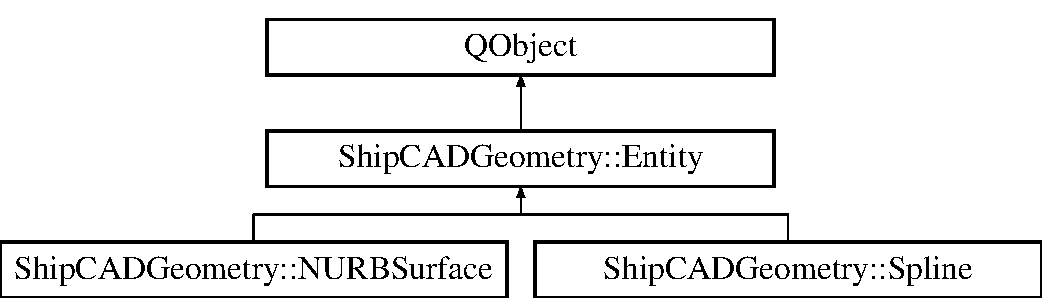
\includegraphics[height=3.000000cm]{classShipCADGeometry_1_1Entity}
\end{center}
\end{figure}
\subsection*{Public Member Functions}
\begin{DoxyCompactItemize}
\item 
\hyperlink{classShipCADGeometry_1_1Entity_a980f368aa07ce358583982821533a54a}{Entity} ()
\item 
virtual \hyperlink{classShipCADGeometry_1_1Entity_a37d42f94118b633fd336c2896f4aae8a}{$\sim$\-Entity} ()
\item 
virtual void \hyperlink{classShipCADGeometry_1_1Entity_a998d0e5d360371046fd5835ba1e0877a}{clear} ()
\item 
virtual void \hyperlink{classShipCADGeometry_1_1Entity_a08e8e53770c85002afa45f46e7bf10f8}{extents} (Q\-Vector3\-D \&min, Q\-Vector3\-D \&max)
\item 
virtual void \hyperlink{classShipCADGeometry_1_1Entity_a894bb00b5f65692c1a64e62d748f4041}{draw} (\hyperlink{classShipCADGeometry_1_1Viewport}{Viewport} \&vp, \hyperlink{classShipCADGeometry_1_1LineShader}{Line\-Shader} $\ast$lineshader)=0
\item 
virtual void \hyperlink{classShipCADGeometry_1_1Entity_ad49217d575c57a1fcc99768081b864ee}{rebuild} ()=0
\item 
Q\-Vector3\-D \hyperlink{classShipCADGeometry_1_1Entity_a759d6dedd36bf6562fbf36e816d9a5af}{get\-Min} ()
\item 
Q\-Vector3\-D \hyperlink{classShipCADGeometry_1_1Entity_a3af98adafb45eb573675a8ccc44fe14e}{get\-Max} ()
\item 
bool \hyperlink{classShipCADGeometry_1_1Entity_a131cd27d923ba1d2658528b679b9a90c}{is\-Build} ()
\item 
void \hyperlink{classShipCADGeometry_1_1Entity_a395d7573df06482d9deaecdc87d46944}{dump} (std\-::ostream \&os) const 
\end{DoxyCompactItemize}
\subsection*{Protected Member Functions}
\begin{DoxyCompactItemize}
\item 
virtual void \hyperlink{classShipCADGeometry_1_1Entity_a1889198398f42bb7f77a2334031c3f33}{set\-Build} (bool val)
\end{DoxyCompactItemize}
\subsection*{Protected Attributes}
\begin{DoxyCompactItemize}
\item 
bool \hyperlink{classShipCADGeometry_1_1Entity_aadcf171a362955d78fd34d8b5919745d}{\-\_\-build}
\item 
Q\-Vector3\-D \hyperlink{classShipCADGeometry_1_1Entity_a873861fe2282f4300ef60c846bd7469e}{\-\_\-min}
\item 
Q\-Vector3\-D \hyperlink{classShipCADGeometry_1_1Entity_a3dc59ce1edbde84e85f1b096466eb497}{\-\_\-max}
\item 
int \hyperlink{classShipCADGeometry_1_1Entity_af9d015ffcbdc506db94c677be5b2f8ec}{\-\_\-pen\-\_\-width}
\item 
Q\-Color \hyperlink{classShipCADGeometry_1_1Entity_a5107c39b85d2fe2cad3d8266a62168ac}{\-\_\-color}
\item 
Qt\-::\-Pen\-Style \hyperlink{classShipCADGeometry_1_1Entity_ab251bdeaec08bb1474ba57725735198a}{\-\_\-pen\-\_\-style}
\end{DoxyCompactItemize}
\subsection*{Properties}
\begin{DoxyCompactItemize}
\item 
bool \hyperlink{classShipCADGeometry_1_1Entity_a9dc2f1b0245a88b3ed9b9b47f626fdb3}{Build}
\item 
Q\-Color \hyperlink{classShipCADGeometry_1_1Entity_a55bb9634ac4c8f08909376006de897b4}{Color}
\item 
Q\-Vector3\-D \hyperlink{classShipCADGeometry_1_1Entity_a3bd95518fc98793471c03637679081a8}{Min}
\item 
Q\-Vector3\-D \hyperlink{classShipCADGeometry_1_1Entity_a9b51589fe54df18ce1ca593de6e8bd1f}{Max}
\item 
int \hyperlink{classShipCADGeometry_1_1Entity_a236c42fc6ed4a8478760baf81551620f}{Pen\-Width}
\item 
Qt\-::\-Pen\-Style \hyperlink{classShipCADGeometry_1_1Entity_adf613c5cb8169e0915f8d15aad664d4a}{penstyle}
\end{DoxyCompactItemize}


\subsection{Detailed Description}


Definition at line 62 of file entity.\-h.



\subsection{Constructor \& Destructor Documentation}
\hypertarget{classShipCADGeometry_1_1Entity_a980f368aa07ce358583982821533a54a}{\index{Ship\-C\-A\-D\-Geometry\-::\-Entity@{Ship\-C\-A\-D\-Geometry\-::\-Entity}!Entity@{Entity}}
\index{Entity@{Entity}!ShipCADGeometry::Entity@{Ship\-C\-A\-D\-Geometry\-::\-Entity}}
\subsubsection[{Entity}]{\setlength{\rightskip}{0pt plus 5cm}Entity\-::\-Entity (
\begin{DoxyParamCaption}
{}
\end{DoxyParamCaption}
)\hspace{0.3cm}{\ttfamily [explicit]}}}\label{classShipCADGeometry_1_1Entity_a980f368aa07ce358583982821533a54a}


Definition at line 43 of file entity.\-cpp.

\hypertarget{classShipCADGeometry_1_1Entity_a37d42f94118b633fd336c2896f4aae8a}{\index{Ship\-C\-A\-D\-Geometry\-::\-Entity@{Ship\-C\-A\-D\-Geometry\-::\-Entity}!$\sim$\-Entity@{$\sim$\-Entity}}
\index{$\sim$\-Entity@{$\sim$\-Entity}!ShipCADGeometry::Entity@{Ship\-C\-A\-D\-Geometry\-::\-Entity}}
\subsubsection[{$\sim$\-Entity}]{\setlength{\rightskip}{0pt plus 5cm}virtual Ship\-C\-A\-D\-Geometry\-::\-Entity\-::$\sim$\-Entity (
\begin{DoxyParamCaption}
{}
\end{DoxyParamCaption}
)\hspace{0.3cm}{\ttfamily [inline]}, {\ttfamily [virtual]}}}\label{classShipCADGeometry_1_1Entity_a37d42f94118b633fd336c2896f4aae8a}


Definition at line 75 of file entity.\-h.



\subsection{Member Function Documentation}
\hypertarget{classShipCADGeometry_1_1Entity_a998d0e5d360371046fd5835ba1e0877a}{\index{Ship\-C\-A\-D\-Geometry\-::\-Entity@{Ship\-C\-A\-D\-Geometry\-::\-Entity}!clear@{clear}}
\index{clear@{clear}!ShipCADGeometry::Entity@{Ship\-C\-A\-D\-Geometry\-::\-Entity}}
\subsubsection[{clear}]{\setlength{\rightskip}{0pt plus 5cm}void Entity\-::clear (
\begin{DoxyParamCaption}
{}
\end{DoxyParamCaption}
)\hspace{0.3cm}{\ttfamily [virtual]}}}\label{classShipCADGeometry_1_1Entity_a998d0e5d360371046fd5835ba1e0877a}


Reimplemented in \hyperlink{classShipCADGeometry_1_1Spline_a02967f3eee8b1755eab0d7da55c3c621}{Ship\-C\-A\-D\-Geometry\-::\-Spline}, and \hyperlink{classShipCADGeometry_1_1NURBSurface_a5013b0c1e511ea68909eef5d0473d032}{Ship\-C\-A\-D\-Geometry\-::\-N\-U\-R\-B\-Surface}.



Definition at line 48 of file entity.\-cpp.

\hypertarget{classShipCADGeometry_1_1Entity_a894bb00b5f65692c1a64e62d748f4041}{\index{Ship\-C\-A\-D\-Geometry\-::\-Entity@{Ship\-C\-A\-D\-Geometry\-::\-Entity}!draw@{draw}}
\index{draw@{draw}!ShipCADGeometry::Entity@{Ship\-C\-A\-D\-Geometry\-::\-Entity}}
\subsubsection[{draw}]{\setlength{\rightskip}{0pt plus 5cm}virtual void Ship\-C\-A\-D\-Geometry\-::\-Entity\-::draw (
\begin{DoxyParamCaption}
\item[{{\bf Viewport} \&}]{vp, }
\item[{{\bf Line\-Shader} $\ast$}]{lineshader}
\end{DoxyParamCaption}
)\hspace{0.3cm}{\ttfamily [pure virtual]}}}\label{classShipCADGeometry_1_1Entity_a894bb00b5f65692c1a64e62d748f4041}


Implemented in \hyperlink{classShipCADGeometry_1_1Spline_a6424ed433d241f566c15891cc25a74dd}{Ship\-C\-A\-D\-Geometry\-::\-Spline}.

\hypertarget{classShipCADGeometry_1_1Entity_a395d7573df06482d9deaecdc87d46944}{\index{Ship\-C\-A\-D\-Geometry\-::\-Entity@{Ship\-C\-A\-D\-Geometry\-::\-Entity}!dump@{dump}}
\index{dump@{dump}!ShipCADGeometry::Entity@{Ship\-C\-A\-D\-Geometry\-::\-Entity}}
\subsubsection[{dump}]{\setlength{\rightskip}{0pt plus 5cm}void Entity\-::dump (
\begin{DoxyParamCaption}
\item[{std\-::ostream \&}]{os}
\end{DoxyParamCaption}
) const}}\label{classShipCADGeometry_1_1Entity_a395d7573df06482d9deaecdc87d46944}


Definition at line 96 of file entity.\-cpp.

\hypertarget{classShipCADGeometry_1_1Entity_a08e8e53770c85002afa45f46e7bf10f8}{\index{Ship\-C\-A\-D\-Geometry\-::\-Entity@{Ship\-C\-A\-D\-Geometry\-::\-Entity}!extents@{extents}}
\index{extents@{extents}!ShipCADGeometry::Entity@{Ship\-C\-A\-D\-Geometry\-::\-Entity}}
\subsubsection[{extents}]{\setlength{\rightskip}{0pt plus 5cm}void Entity\-::extents (
\begin{DoxyParamCaption}
\item[{Q\-Vector3\-D \&}]{min, }
\item[{Q\-Vector3\-D \&}]{max}
\end{DoxyParamCaption}
)\hspace{0.3cm}{\ttfamily [virtual]}}}\label{classShipCADGeometry_1_1Entity_a08e8e53770c85002afa45f46e7bf10f8}


Definition at line 58 of file entity.\-cpp.

\hypertarget{classShipCADGeometry_1_1Entity_a3af98adafb45eb573675a8ccc44fe14e}{\index{Ship\-C\-A\-D\-Geometry\-::\-Entity@{Ship\-C\-A\-D\-Geometry\-::\-Entity}!get\-Max@{get\-Max}}
\index{get\-Max@{get\-Max}!ShipCADGeometry::Entity@{Ship\-C\-A\-D\-Geometry\-::\-Entity}}
\subsubsection[{get\-Max}]{\setlength{\rightskip}{0pt plus 5cm}Q\-Vector3\-D Entity\-::get\-Max (
\begin{DoxyParamCaption}
{}
\end{DoxyParamCaption}
)}}\label{classShipCADGeometry_1_1Entity_a3af98adafb45eb573675a8ccc44fe14e}


Definition at line 89 of file entity.\-cpp.

\hypertarget{classShipCADGeometry_1_1Entity_a759d6dedd36bf6562fbf36e816d9a5af}{\index{Ship\-C\-A\-D\-Geometry\-::\-Entity@{Ship\-C\-A\-D\-Geometry\-::\-Entity}!get\-Min@{get\-Min}}
\index{get\-Min@{get\-Min}!ShipCADGeometry::Entity@{Ship\-C\-A\-D\-Geometry\-::\-Entity}}
\subsubsection[{get\-Min}]{\setlength{\rightskip}{0pt plus 5cm}Q\-Vector3\-D Entity\-::get\-Min (
\begin{DoxyParamCaption}
{}
\end{DoxyParamCaption}
)}}\label{classShipCADGeometry_1_1Entity_a759d6dedd36bf6562fbf36e816d9a5af}


Definition at line 82 of file entity.\-cpp.

\hypertarget{classShipCADGeometry_1_1Entity_a131cd27d923ba1d2658528b679b9a90c}{\index{Ship\-C\-A\-D\-Geometry\-::\-Entity@{Ship\-C\-A\-D\-Geometry\-::\-Entity}!is\-Build@{is\-Build}}
\index{is\-Build@{is\-Build}!ShipCADGeometry::Entity@{Ship\-C\-A\-D\-Geometry\-::\-Entity}}
\subsubsection[{is\-Build}]{\setlength{\rightskip}{0pt plus 5cm}bool Entity\-::is\-Build (
\begin{DoxyParamCaption}
{}
\end{DoxyParamCaption}
)}}\label{classShipCADGeometry_1_1Entity_a131cd27d923ba1d2658528b679b9a90c}


Definition at line 66 of file entity.\-cpp.

\hypertarget{classShipCADGeometry_1_1Entity_ad49217d575c57a1fcc99768081b864ee}{\index{Ship\-C\-A\-D\-Geometry\-::\-Entity@{Ship\-C\-A\-D\-Geometry\-::\-Entity}!rebuild@{rebuild}}
\index{rebuild@{rebuild}!ShipCADGeometry::Entity@{Ship\-C\-A\-D\-Geometry\-::\-Entity}}
\subsubsection[{rebuild}]{\setlength{\rightskip}{0pt plus 5cm}virtual void Ship\-C\-A\-D\-Geometry\-::\-Entity\-::rebuild (
\begin{DoxyParamCaption}
{}
\end{DoxyParamCaption}
)\hspace{0.3cm}{\ttfamily [pure virtual]}}}\label{classShipCADGeometry_1_1Entity_ad49217d575c57a1fcc99768081b864ee}


Implemented in \hyperlink{classShipCADGeometry_1_1Spline_a9b466ad7510032dafb0421f2d834bde6}{Ship\-C\-A\-D\-Geometry\-::\-Spline}, and \hyperlink{classShipCADGeometry_1_1NURBSurface_a643231ea9a8f26e528a1d9a0dccf4070}{Ship\-C\-A\-D\-Geometry\-::\-N\-U\-R\-B\-Surface}.

\hypertarget{classShipCADGeometry_1_1Entity_a1889198398f42bb7f77a2334031c3f33}{\index{Ship\-C\-A\-D\-Geometry\-::\-Entity@{Ship\-C\-A\-D\-Geometry\-::\-Entity}!set\-Build@{set\-Build}}
\index{set\-Build@{set\-Build}!ShipCADGeometry::Entity@{Ship\-C\-A\-D\-Geometry\-::\-Entity}}
\subsubsection[{set\-Build}]{\setlength{\rightskip}{0pt plus 5cm}void Entity\-::set\-Build (
\begin{DoxyParamCaption}
\item[{bool}]{val}
\end{DoxyParamCaption}
)\hspace{0.3cm}{\ttfamily [protected]}, {\ttfamily [virtual]}}}\label{classShipCADGeometry_1_1Entity_a1889198398f42bb7f77a2334031c3f33}


Reimplemented in \hyperlink{classShipCADGeometry_1_1Spline_a6e932411f0f4463514f80011c58f5e6a}{Ship\-C\-A\-D\-Geometry\-::\-Spline}, and \hyperlink{classShipCADGeometry_1_1NURBSurface_aa6fc3d060087593349ce1b5119419433}{Ship\-C\-A\-D\-Geometry\-::\-N\-U\-R\-B\-Surface}.



Definition at line 71 of file entity.\-cpp.



\subsection{Member Data Documentation}
\hypertarget{classShipCADGeometry_1_1Entity_aadcf171a362955d78fd34d8b5919745d}{\index{Ship\-C\-A\-D\-Geometry\-::\-Entity@{Ship\-C\-A\-D\-Geometry\-::\-Entity}!\-\_\-build@{\-\_\-build}}
\index{\-\_\-build@{\-\_\-build}!ShipCADGeometry::Entity@{Ship\-C\-A\-D\-Geometry\-::\-Entity}}
\subsubsection[{\-\_\-build}]{\setlength{\rightskip}{0pt plus 5cm}bool Ship\-C\-A\-D\-Geometry\-::\-Entity\-::\-\_\-build\hspace{0.3cm}{\ttfamily [protected]}}}\label{classShipCADGeometry_1_1Entity_aadcf171a362955d78fd34d8b5919745d}


Definition at line 96 of file entity.\-h.

\hypertarget{classShipCADGeometry_1_1Entity_a5107c39b85d2fe2cad3d8266a62168ac}{\index{Ship\-C\-A\-D\-Geometry\-::\-Entity@{Ship\-C\-A\-D\-Geometry\-::\-Entity}!\-\_\-color@{\-\_\-color}}
\index{\-\_\-color@{\-\_\-color}!ShipCADGeometry::Entity@{Ship\-C\-A\-D\-Geometry\-::\-Entity}}
\subsubsection[{\-\_\-color}]{\setlength{\rightskip}{0pt plus 5cm}Q\-Color Ship\-C\-A\-D\-Geometry\-::\-Entity\-::\-\_\-color\hspace{0.3cm}{\ttfamily [protected]}}}\label{classShipCADGeometry_1_1Entity_a5107c39b85d2fe2cad3d8266a62168ac}


Definition at line 100 of file entity.\-h.

\hypertarget{classShipCADGeometry_1_1Entity_a3dc59ce1edbde84e85f1b096466eb497}{\index{Ship\-C\-A\-D\-Geometry\-::\-Entity@{Ship\-C\-A\-D\-Geometry\-::\-Entity}!\-\_\-max@{\-\_\-max}}
\index{\-\_\-max@{\-\_\-max}!ShipCADGeometry::Entity@{Ship\-C\-A\-D\-Geometry\-::\-Entity}}
\subsubsection[{\-\_\-max}]{\setlength{\rightskip}{0pt plus 5cm}Q\-Vector3\-D Ship\-C\-A\-D\-Geometry\-::\-Entity\-::\-\_\-max\hspace{0.3cm}{\ttfamily [protected]}}}\label{classShipCADGeometry_1_1Entity_a3dc59ce1edbde84e85f1b096466eb497}


Definition at line 98 of file entity.\-h.

\hypertarget{classShipCADGeometry_1_1Entity_a873861fe2282f4300ef60c846bd7469e}{\index{Ship\-C\-A\-D\-Geometry\-::\-Entity@{Ship\-C\-A\-D\-Geometry\-::\-Entity}!\-\_\-min@{\-\_\-min}}
\index{\-\_\-min@{\-\_\-min}!ShipCADGeometry::Entity@{Ship\-C\-A\-D\-Geometry\-::\-Entity}}
\subsubsection[{\-\_\-min}]{\setlength{\rightskip}{0pt plus 5cm}Q\-Vector3\-D Ship\-C\-A\-D\-Geometry\-::\-Entity\-::\-\_\-min\hspace{0.3cm}{\ttfamily [protected]}}}\label{classShipCADGeometry_1_1Entity_a873861fe2282f4300ef60c846bd7469e}


Definition at line 97 of file entity.\-h.

\hypertarget{classShipCADGeometry_1_1Entity_ab251bdeaec08bb1474ba57725735198a}{\index{Ship\-C\-A\-D\-Geometry\-::\-Entity@{Ship\-C\-A\-D\-Geometry\-::\-Entity}!\-\_\-pen\-\_\-style@{\-\_\-pen\-\_\-style}}
\index{\-\_\-pen\-\_\-style@{\-\_\-pen\-\_\-style}!ShipCADGeometry::Entity@{Ship\-C\-A\-D\-Geometry\-::\-Entity}}
\subsubsection[{\-\_\-pen\-\_\-style}]{\setlength{\rightskip}{0pt plus 5cm}Qt\-::\-Pen\-Style Ship\-C\-A\-D\-Geometry\-::\-Entity\-::\-\_\-pen\-\_\-style\hspace{0.3cm}{\ttfamily [protected]}}}\label{classShipCADGeometry_1_1Entity_ab251bdeaec08bb1474ba57725735198a}


Definition at line 101 of file entity.\-h.

\hypertarget{classShipCADGeometry_1_1Entity_af9d015ffcbdc506db94c677be5b2f8ec}{\index{Ship\-C\-A\-D\-Geometry\-::\-Entity@{Ship\-C\-A\-D\-Geometry\-::\-Entity}!\-\_\-pen\-\_\-width@{\-\_\-pen\-\_\-width}}
\index{\-\_\-pen\-\_\-width@{\-\_\-pen\-\_\-width}!ShipCADGeometry::Entity@{Ship\-C\-A\-D\-Geometry\-::\-Entity}}
\subsubsection[{\-\_\-pen\-\_\-width}]{\setlength{\rightskip}{0pt plus 5cm}int Ship\-C\-A\-D\-Geometry\-::\-Entity\-::\-\_\-pen\-\_\-width\hspace{0.3cm}{\ttfamily [protected]}}}\label{classShipCADGeometry_1_1Entity_af9d015ffcbdc506db94c677be5b2f8ec}


Definition at line 99 of file entity.\-h.



\subsection{Property Documentation}
\hypertarget{classShipCADGeometry_1_1Entity_a9dc2f1b0245a88b3ed9b9b47f626fdb3}{\index{Ship\-C\-A\-D\-Geometry\-::\-Entity@{Ship\-C\-A\-D\-Geometry\-::\-Entity}!Build@{Build}}
\index{Build@{Build}!ShipCADGeometry::Entity@{Ship\-C\-A\-D\-Geometry\-::\-Entity}}
\subsubsection[{Build}]{\setlength{\rightskip}{0pt plus 5cm}bool Ship\-C\-A\-D\-Geometry\-::\-Entity\-::\-Build\hspace{0.3cm}{\ttfamily [read]}}}\label{classShipCADGeometry_1_1Entity_a9dc2f1b0245a88b3ed9b9b47f626fdb3}


Definition at line 65 of file entity.\-h.

\hypertarget{classShipCADGeometry_1_1Entity_a55bb9634ac4c8f08909376006de897b4}{\index{Ship\-C\-A\-D\-Geometry\-::\-Entity@{Ship\-C\-A\-D\-Geometry\-::\-Entity}!Color@{Color}}
\index{Color@{Color}!ShipCADGeometry::Entity@{Ship\-C\-A\-D\-Geometry\-::\-Entity}}
\subsubsection[{Color}]{\setlength{\rightskip}{0pt plus 5cm}Q\-Color Ship\-C\-A\-D\-Geometry\-::\-Entity\-::\-Color}}\label{classShipCADGeometry_1_1Entity_a55bb9634ac4c8f08909376006de897b4}


Definition at line 66 of file entity.\-h.

\hypertarget{classShipCADGeometry_1_1Entity_a9b51589fe54df18ce1ca593de6e8bd1f}{\index{Ship\-C\-A\-D\-Geometry\-::\-Entity@{Ship\-C\-A\-D\-Geometry\-::\-Entity}!Max@{Max}}
\index{Max@{Max}!ShipCADGeometry::Entity@{Ship\-C\-A\-D\-Geometry\-::\-Entity}}
\subsubsection[{Max}]{\setlength{\rightskip}{0pt plus 5cm}Q\-Vector3\-D Ship\-C\-A\-D\-Geometry\-::\-Entity\-::\-Max\hspace{0.3cm}{\ttfamily [read]}}}\label{classShipCADGeometry_1_1Entity_a9b51589fe54df18ce1ca593de6e8bd1f}


Definition at line 68 of file entity.\-h.

\hypertarget{classShipCADGeometry_1_1Entity_a3bd95518fc98793471c03637679081a8}{\index{Ship\-C\-A\-D\-Geometry\-::\-Entity@{Ship\-C\-A\-D\-Geometry\-::\-Entity}!Min@{Min}}
\index{Min@{Min}!ShipCADGeometry::Entity@{Ship\-C\-A\-D\-Geometry\-::\-Entity}}
\subsubsection[{Min}]{\setlength{\rightskip}{0pt plus 5cm}Q\-Vector3\-D Ship\-C\-A\-D\-Geometry\-::\-Entity\-::\-Min\hspace{0.3cm}{\ttfamily [read]}}}\label{classShipCADGeometry_1_1Entity_a3bd95518fc98793471c03637679081a8}


Definition at line 67 of file entity.\-h.

\hypertarget{classShipCADGeometry_1_1Entity_adf613c5cb8169e0915f8d15aad664d4a}{\index{Ship\-C\-A\-D\-Geometry\-::\-Entity@{Ship\-C\-A\-D\-Geometry\-::\-Entity}!penstyle@{penstyle}}
\index{penstyle@{penstyle}!ShipCADGeometry::Entity@{Ship\-C\-A\-D\-Geometry\-::\-Entity}}
\subsubsection[{penstyle}]{\setlength{\rightskip}{0pt plus 5cm}Qt\-::\-Pen\-Style Ship\-C\-A\-D\-Geometry\-::\-Entity\-::penstyle}}\label{classShipCADGeometry_1_1Entity_adf613c5cb8169e0915f8d15aad664d4a}


Definition at line 70 of file entity.\-h.

\hypertarget{classShipCADGeometry_1_1Entity_a236c42fc6ed4a8478760baf81551620f}{\index{Ship\-C\-A\-D\-Geometry\-::\-Entity@{Ship\-C\-A\-D\-Geometry\-::\-Entity}!Pen\-Width@{Pen\-Width}}
\index{Pen\-Width@{Pen\-Width}!ShipCADGeometry::Entity@{Ship\-C\-A\-D\-Geometry\-::\-Entity}}
\subsubsection[{Pen\-Width}]{\setlength{\rightskip}{0pt plus 5cm}int Ship\-C\-A\-D\-Geometry\-::\-Entity\-::\-Pen\-Width}}\label{classShipCADGeometry_1_1Entity_a236c42fc6ed4a8478760baf81551620f}


Definition at line 69 of file entity.\-h.



The documentation for this class was generated from the following files\-:\begin{DoxyCompactItemize}
\item 
Ship\-C\-A\-Dlib/\hyperlink{entity_8h}{entity.\-h}\item 
Ship\-C\-A\-Dlib/\hyperlink{entity_8cpp}{entity.\-cpp}\end{DoxyCompactItemize}

\hypertarget{structExistPointPred}{\section{Exist\-Point\-Pred Struct Reference}
\label{structExistPointPred}\index{Exist\-Point\-Pred@{Exist\-Point\-Pred}}
}
\subsection*{Public Member Functions}
\begin{DoxyCompactItemize}
\item 
bool \hyperlink{structExistPointPred_a349fa048c84af089053c09f0ac76325b}{operator()} (const pair$<$ \hyperlink{classShipCAD_1_1SubdivisionControlPoint}{Ship\-C\-A\-D\-::\-Subdivision\-Control\-Point} $\ast$, \hyperlink{classShipCAD_1_1SubdivisionControlPoint}{Ship\-C\-A\-D\-::\-Subdivision\-Control\-Point} $\ast$ $>$ \&val)
\item 
\hyperlink{structExistPointPred_a7e596a35605dc5f710f6ea9a2e07eed2}{Exist\-Point\-Pred} (\hyperlink{classShipCAD_1_1SubdivisionPoint}{Ship\-C\-A\-D\-::\-Subdivision\-Point} $\ast$querypt)
\end{DoxyCompactItemize}
\subsection*{Public Attributes}
\begin{DoxyCompactItemize}
\item 
\hyperlink{classShipCAD_1_1SubdivisionControlPoint}{Ship\-C\-A\-D\-::\-Subdivision\-Control\-Point} $\ast$ \hyperlink{structExistPointPred_a237f009691af455ff164985c3ab80901}{\-\_\-querypt}
\end{DoxyCompactItemize}


\subsection{Detailed Description}


Definition at line 1396 of file subdivsurface.\-cpp.



\subsection{Constructor \& Destructor Documentation}
\hypertarget{structExistPointPred_a7e596a35605dc5f710f6ea9a2e07eed2}{\index{Exist\-Point\-Pred@{Exist\-Point\-Pred}!Exist\-Point\-Pred@{Exist\-Point\-Pred}}
\index{Exist\-Point\-Pred@{Exist\-Point\-Pred}!ExistPointPred@{Exist\-Point\-Pred}}
\subsubsection[{Exist\-Point\-Pred}]{\setlength{\rightskip}{0pt plus 5cm}Exist\-Point\-Pred\-::\-Exist\-Point\-Pred (
\begin{DoxyParamCaption}
\item[{{\bf Ship\-C\-A\-D\-::\-Subdivision\-Point} $\ast$}]{querypt}
\end{DoxyParamCaption}
)\hspace{0.3cm}{\ttfamily [inline]}}}\label{structExistPointPred_a7e596a35605dc5f710f6ea9a2e07eed2}


Definition at line 1402 of file subdivsurface.\-cpp.



\subsection{Member Function Documentation}
\hypertarget{structExistPointPred_a349fa048c84af089053c09f0ac76325b}{\index{Exist\-Point\-Pred@{Exist\-Point\-Pred}!operator()@{operator()}}
\index{operator()@{operator()}!ExistPointPred@{Exist\-Point\-Pred}}
\subsubsection[{operator()}]{\setlength{\rightskip}{0pt plus 5cm}bool Exist\-Point\-Pred\-::operator() (
\begin{DoxyParamCaption}
\item[{const pair$<$ {\bf Ship\-C\-A\-D\-::\-Subdivision\-Control\-Point} $\ast$, {\bf Ship\-C\-A\-D\-::\-Subdivision\-Control\-Point} $\ast$ $>$ \&}]{val}
\end{DoxyParamCaption}
)\hspace{0.3cm}{\ttfamily [inline]}}}\label{structExistPointPred_a349fa048c84af089053c09f0ac76325b}


Definition at line 1398 of file subdivsurface.\-cpp.



\subsection{Member Data Documentation}
\hypertarget{structExistPointPred_a237f009691af455ff164985c3ab80901}{\index{Exist\-Point\-Pred@{Exist\-Point\-Pred}!\-\_\-querypt@{\-\_\-querypt}}
\index{\-\_\-querypt@{\-\_\-querypt}!ExistPointPred@{Exist\-Point\-Pred}}
\subsubsection[{\-\_\-querypt}]{\setlength{\rightskip}{0pt plus 5cm}{\bf Ship\-C\-A\-D\-::\-Subdivision\-Control\-Point}$\ast$ Exist\-Point\-Pred\-::\-\_\-querypt}}\label{structExistPointPred_a237f009691af455ff164985c3ab80901}


Definition at line 1397 of file subdivsurface.\-cpp.



The documentation for this struct was generated from the following file\-:\begin{DoxyCompactItemize}
\item 
Ship\-C\-A\-Dlib/\hyperlink{subdivsurface_8cpp}{subdivsurface.\-cpp}\end{DoxyCompactItemize}

\hypertarget{structExtrudePointPred}{\section{Extrude\-Point\-Pred Struct Reference}
\label{structExtrudePointPred}\index{Extrude\-Point\-Pred@{Extrude\-Point\-Pred}}
}
\subsection*{Public Member Functions}
\begin{DoxyCompactItemize}
\item 
bool \hyperlink{structExtrudePointPred_ab8901a2a46f147e81c80c25b0492c772}{operator()} (const pair$<$ \hyperlink{classShipCAD_1_1SubdivisionControlPoint}{Ship\-C\-A\-D\-::\-Subdivision\-Control\-Point} $\ast$, \hyperlink{classShipCAD_1_1SubdivisionControlPoint}{Ship\-C\-A\-D\-::\-Subdivision\-Control\-Point} $\ast$ $>$ \&val)
\item 
\hyperlink{structExtrudePointPred_ac213b3b8d1bdc5a72e0a5a4ed53d9439}{Extrude\-Point\-Pred} (\hyperlink{classShipCAD_1_1SubdivisionPoint}{Ship\-C\-A\-D\-::\-Subdivision\-Point} $\ast$querypt)
\end{DoxyCompactItemize}
\subsection*{Public Attributes}
\begin{DoxyCompactItemize}
\item 
\hyperlink{classShipCAD_1_1SubdivisionControlPoint}{Ship\-C\-A\-D\-::\-Subdivision\-Control\-Point} $\ast$ \hyperlink{structExtrudePointPred_af9fa40238ef74aca6b8f8d7e303aafb4}{\-\_\-querypt}
\end{DoxyCompactItemize}


\subsection{Detailed Description}


Definition at line 1941 of file subdivsurface.\-cpp.



\subsection{Constructor \& Destructor Documentation}
\hypertarget{structExtrudePointPred_ac213b3b8d1bdc5a72e0a5a4ed53d9439}{\index{Extrude\-Point\-Pred@{Extrude\-Point\-Pred}!Extrude\-Point\-Pred@{Extrude\-Point\-Pred}}
\index{Extrude\-Point\-Pred@{Extrude\-Point\-Pred}!ExtrudePointPred@{Extrude\-Point\-Pred}}
\subsubsection[{Extrude\-Point\-Pred}]{\setlength{\rightskip}{0pt plus 5cm}Extrude\-Point\-Pred\-::\-Extrude\-Point\-Pred (
\begin{DoxyParamCaption}
\item[{{\bf Ship\-C\-A\-D\-::\-Subdivision\-Point} $\ast$}]{querypt}
\end{DoxyParamCaption}
)\hspace{0.3cm}{\ttfamily [inline]}}}\label{structExtrudePointPred_ac213b3b8d1bdc5a72e0a5a4ed53d9439}


Definition at line 1947 of file subdivsurface.\-cpp.



\subsection{Member Function Documentation}
\hypertarget{structExtrudePointPred_ab8901a2a46f147e81c80c25b0492c772}{\index{Extrude\-Point\-Pred@{Extrude\-Point\-Pred}!operator()@{operator()}}
\index{operator()@{operator()}!ExtrudePointPred@{Extrude\-Point\-Pred}}
\subsubsection[{operator()}]{\setlength{\rightskip}{0pt plus 5cm}bool Extrude\-Point\-Pred\-::operator() (
\begin{DoxyParamCaption}
\item[{const pair$<$ {\bf Ship\-C\-A\-D\-::\-Subdivision\-Control\-Point} $\ast$, {\bf Ship\-C\-A\-D\-::\-Subdivision\-Control\-Point} $\ast$ $>$ \&}]{val}
\end{DoxyParamCaption}
)\hspace{0.3cm}{\ttfamily [inline]}}}\label{structExtrudePointPred_ab8901a2a46f147e81c80c25b0492c772}


Definition at line 1943 of file subdivsurface.\-cpp.



\subsection{Member Data Documentation}
\hypertarget{structExtrudePointPred_af9fa40238ef74aca6b8f8d7e303aafb4}{\index{Extrude\-Point\-Pred@{Extrude\-Point\-Pred}!\-\_\-querypt@{\-\_\-querypt}}
\index{\-\_\-querypt@{\-\_\-querypt}!ExtrudePointPred@{Extrude\-Point\-Pred}}
\subsubsection[{\-\_\-querypt}]{\setlength{\rightskip}{0pt plus 5cm}{\bf Ship\-C\-A\-D\-::\-Subdivision\-Control\-Point}$\ast$ Extrude\-Point\-Pred\-::\-\_\-querypt}}\label{structExtrudePointPred_af9fa40238ef74aca6b8f8d7e303aafb4}


Definition at line 1942 of file subdivsurface.\-cpp.



The documentation for this struct was generated from the following file\-:\begin{DoxyCompactItemize}
\item 
Ship\-C\-A\-Dlib/\hyperlink{subdivsurface_8cpp}{subdivsurface.\-cpp}\end{DoxyCompactItemize}

\hypertarget{structFacePred}{\section{Face\-Pred Struct Reference}
\label{structFacePred}\index{Face\-Pred@{Face\-Pred}}
}
\subsection*{Public Member Functions}
\begin{DoxyCompactItemize}
\item 
bool \hyperlink{structFacePred_a6abdd4cf5e1665459109f92abbba8e43}{operator()} (const pair$<$ \hyperlink{classShipCAD_1_1SubdivisionFace}{Ship\-C\-A\-D\-::\-Subdivision\-Face} $\ast$, \hyperlink{classShipCAD_1_1SubdivisionPoint}{Ship\-C\-A\-D\-::\-Subdivision\-Point} $\ast$ $>$ \&val)
\item 
\hyperlink{structFacePred_a8ce3462c74c45932241e934da4048a65}{Face\-Pred} (\hyperlink{classShipCAD_1_1SubdivisionFace}{Ship\-C\-A\-D\-::\-Subdivision\-Face} $\ast$queryface)
\end{DoxyCompactItemize}
\subsection*{Public Attributes}
\begin{DoxyCompactItemize}
\item 
\hyperlink{classShipCAD_1_1SubdivisionFace}{Ship\-C\-A\-D\-::\-Subdivision\-Face} $\ast$ \hyperlink{structFacePred_abe2d14d3f749323559d7a06b06ca99a8}{\-\_\-queryface}
\end{DoxyCompactItemize}


\subsection{Detailed Description}


Definition at line 239 of file subdivface.\-cpp.



\subsection{Constructor \& Destructor Documentation}
\hypertarget{structFacePred_a8ce3462c74c45932241e934da4048a65}{\index{Face\-Pred@{Face\-Pred}!Face\-Pred@{Face\-Pred}}
\index{Face\-Pred@{Face\-Pred}!FacePred@{Face\-Pred}}
\subsubsection[{Face\-Pred}]{\setlength{\rightskip}{0pt plus 5cm}Face\-Pred\-::\-Face\-Pred (
\begin{DoxyParamCaption}
\item[{{\bf Ship\-C\-A\-D\-::\-Subdivision\-Face} $\ast$}]{queryface}
\end{DoxyParamCaption}
)\hspace{0.3cm}{\ttfamily [inline]}}}\label{structFacePred_a8ce3462c74c45932241e934da4048a65}


Definition at line 245 of file subdivface.\-cpp.



\subsection{Member Function Documentation}
\hypertarget{structFacePred_a6abdd4cf5e1665459109f92abbba8e43}{\index{Face\-Pred@{Face\-Pred}!operator()@{operator()}}
\index{operator()@{operator()}!FacePred@{Face\-Pred}}
\subsubsection[{operator()}]{\setlength{\rightskip}{0pt plus 5cm}bool Face\-Pred\-::operator() (
\begin{DoxyParamCaption}
\item[{const pair$<$ {\bf Ship\-C\-A\-D\-::\-Subdivision\-Face} $\ast$, {\bf Ship\-C\-A\-D\-::\-Subdivision\-Point} $\ast$ $>$ \&}]{val}
\end{DoxyParamCaption}
)\hspace{0.3cm}{\ttfamily [inline]}}}\label{structFacePred_a6abdd4cf5e1665459109f92abbba8e43}


Definition at line 241 of file subdivface.\-cpp.



\subsection{Member Data Documentation}
\hypertarget{structFacePred_abe2d14d3f749323559d7a06b06ca99a8}{\index{Face\-Pred@{Face\-Pred}!\-\_\-queryface@{\-\_\-queryface}}
\index{\-\_\-queryface@{\-\_\-queryface}!FacePred@{Face\-Pred}}
\subsubsection[{\-\_\-queryface}]{\setlength{\rightskip}{0pt plus 5cm}{\bf Ship\-C\-A\-D\-::\-Subdivision\-Face}$\ast$ Face\-Pred\-::\-\_\-queryface}}\label{structFacePred_abe2d14d3f749323559d7a06b06ca99a8}


Definition at line 240 of file subdivface.\-cpp.



The documentation for this struct was generated from the following file\-:\begin{DoxyCompactItemize}
\item 
Ship\-C\-A\-Dlib/\hyperlink{subdivface_8cpp}{subdivface.\-cpp}\end{DoxyCompactItemize}

\hypertarget{classShipCADGeometry_1_1FileBuffer}{\section{Ship\-C\-A\-D\-Geometry\-:\-:File\-Buffer Class Reference}
\label{classShipCADGeometry_1_1FileBuffer}\index{Ship\-C\-A\-D\-Geometry\-::\-File\-Buffer@{Ship\-C\-A\-D\-Geometry\-::\-File\-Buffer}}
}


{\ttfamily \#include $<$filebuffer.\-h$>$}

Inheritance diagram for Ship\-C\-A\-D\-Geometry\-:\-:File\-Buffer\-:\begin{figure}[H]
\begin{center}
\leavevmode
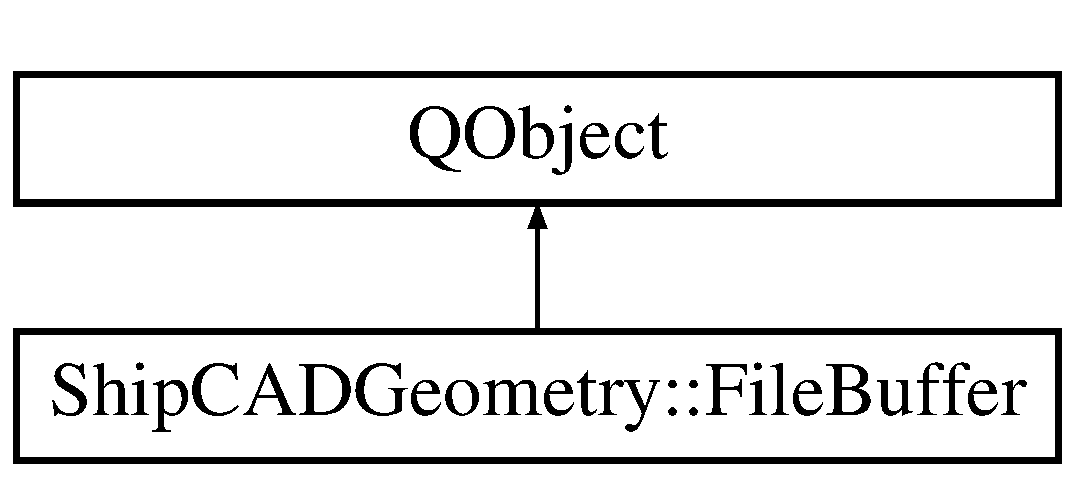
\includegraphics[height=2.000000cm]{classShipCADGeometry_1_1FileBuffer}
\end{center}
\end{figure}
\subsection*{Public Member Functions}
\begin{DoxyCompactItemize}
\item 
\hyperlink{classShipCADGeometry_1_1FileBuffer_ab243cfcb8a68ce791103594e974ee9ba}{File\-Buffer} ()
\item 
\hyperlink{classShipCADGeometry_1_1FileBuffer_ac92d5e7d145ea18fc6a3a6a18c788ebb}{$\sim$\-File\-Buffer} ()
\item 
\hyperlink{namespaceShipCADGeometry_aa8b61644e46115e9d63667f213045e97}{version\-\_\-t} \hyperlink{classShipCADGeometry_1_1FileBuffer_ace63be89e9b23f3ea9a1e93001314d42}{version} ()
\item 
void \hyperlink{classShipCADGeometry_1_1FileBuffer_a7d5d6ac5aa85545999186f4745a77093}{load\-From\-File} (const Q\-String \&filename)
\item 
void \hyperlink{classShipCADGeometry_1_1FileBuffer_a175d7a153228b5cba5db062a2afd5026}{save\-To\-File} (const Q\-String \&filename)
\item 
void \hyperlink{classShipCADGeometry_1_1FileBuffer_af59c26297994b38aabc4bc678d04c246}{reset} ()
\item 
void \hyperlink{classShipCADGeometry_1_1FileBuffer_ad1aebcc97e364569934c66eec5a87485}{load} (bool \&val)
\item 
void \hyperlink{classShipCADGeometry_1_1FileBuffer_a7cb4395eae7ffa405290c3bed9890bee}{add} (bool val)
\item 
void \hyperlink{classShipCADGeometry_1_1FileBuffer_a525306d68a017ef67ec13c3e8901a8ff}{load} (float \&val)
\item 
void \hyperlink{classShipCADGeometry_1_1FileBuffer_a7909794ac33ad5f695bb670940db99ba}{add} (float val)
\item 
void \hyperlink{classShipCADGeometry_1_1FileBuffer_a557fd80268788313b97149797dc710f8}{load} (int \&val)
\item 
void \hyperlink{classShipCADGeometry_1_1FileBuffer_a475ac244828b4ec9bf6e19f1d65e9443}{add} (int val)
\item 
void \hyperlink{classShipCADGeometry_1_1FileBuffer_a10729a5ec1869b76101e52db5a0e3ea7}{load} (size\-\_\-t \&val)
\item 
void \hyperlink{classShipCADGeometry_1_1FileBuffer_aa22983fa24559f6d0d119d89036100af}{add} (size\-\_\-t val)
\item 
void \hyperlink{classShipCADGeometry_1_1FileBuffer_a20977e9b9504c3c5f4cb32adf9ef4659}{load} (\hyperlink{namespaceShipCADGeometry_aa8b61644e46115e9d63667f213045e97}{version\-\_\-t} \&val)
\item 
void \hyperlink{classShipCADGeometry_1_1FileBuffer_a02d5339844191112062d92c9ac74ec96}{add} (\hyperlink{namespaceShipCADGeometry_aa8b61644e46115e9d63667f213045e97}{version\-\_\-t} val)
\item 
void \hyperlink{classShipCADGeometry_1_1FileBuffer_a7255342a053689ebafda9317cc586c57}{load} (Q\-Vector3\-D \&val)
\item 
void \hyperlink{classShipCADGeometry_1_1FileBuffer_a0642733d14682981c12f6aeaef9bb884}{add} (const Q\-Vector3\-D \&val)
\item 
void \hyperlink{classShipCADGeometry_1_1FileBuffer_a3329cf81740c79967acc24bc0ac3c9a3}{load} (Q\-Color \&val)
\item 
void \hyperlink{classShipCADGeometry_1_1FileBuffer_a3611327a77cc938e987ecda018d0d936}{add} (const Q\-Color \&val)
\item 
void \hyperlink{classShipCADGeometry_1_1FileBuffer_a82c790d09c8e85c0f9d218efd9c93605}{load} (Q\-String \&val)
\item 
void \hyperlink{classShipCADGeometry_1_1FileBuffer_aea305be34bc316cc5b849fb291499012}{add} (const Q\-String \&val)
\item 
void \hyperlink{classShipCADGeometry_1_1FileBuffer_a0266bca4cc21cf21bf3802d07ab0f7a4}{load} (\hyperlink{classShipCADGeometry_1_1Plane}{Ship\-C\-A\-D\-Geometry\-::\-Plane} \&val)
\item 
void \hyperlink{classShipCADGeometry_1_1FileBuffer_a0f37901eafb6f12f095ab8389abf3f70}{add} (const \hyperlink{classShipCADGeometry_1_1Plane}{Ship\-C\-A\-D\-Geometry\-::\-Plane} \&val)
\end{DoxyCompactItemize}


\subsection{Detailed Description}


Definition at line 47 of file filebuffer.\-h.



\subsection{Constructor \& Destructor Documentation}
\hypertarget{classShipCADGeometry_1_1FileBuffer_ab243cfcb8a68ce791103594e974ee9ba}{\index{Ship\-C\-A\-D\-Geometry\-::\-File\-Buffer@{Ship\-C\-A\-D\-Geometry\-::\-File\-Buffer}!File\-Buffer@{File\-Buffer}}
\index{File\-Buffer@{File\-Buffer}!ShipCADGeometry::FileBuffer@{Ship\-C\-A\-D\-Geometry\-::\-File\-Buffer}}
\subsubsection[{File\-Buffer}]{\setlength{\rightskip}{0pt plus 5cm}File\-Buffer\-::\-File\-Buffer (
\begin{DoxyParamCaption}
{}
\end{DoxyParamCaption}
)\hspace{0.3cm}{\ttfamily [explicit]}}}\label{classShipCADGeometry_1_1FileBuffer_ab243cfcb8a68ce791103594e974ee9ba}


Definition at line 48 of file filebuffer.\-cpp.

\hypertarget{classShipCADGeometry_1_1FileBuffer_ac92d5e7d145ea18fc6a3a6a18c788ebb}{\index{Ship\-C\-A\-D\-Geometry\-::\-File\-Buffer@{Ship\-C\-A\-D\-Geometry\-::\-File\-Buffer}!$\sim$\-File\-Buffer@{$\sim$\-File\-Buffer}}
\index{$\sim$\-File\-Buffer@{$\sim$\-File\-Buffer}!ShipCADGeometry::FileBuffer@{Ship\-C\-A\-D\-Geometry\-::\-File\-Buffer}}
\subsubsection[{$\sim$\-File\-Buffer}]{\setlength{\rightskip}{0pt plus 5cm}File\-Buffer\-::$\sim$\-File\-Buffer (
\begin{DoxyParamCaption}
{}
\end{DoxyParamCaption}
)}}\label{classShipCADGeometry_1_1FileBuffer_ac92d5e7d145ea18fc6a3a6a18c788ebb}


Definition at line 54 of file filebuffer.\-cpp.



\subsection{Member Function Documentation}
\hypertarget{classShipCADGeometry_1_1FileBuffer_a7cb4395eae7ffa405290c3bed9890bee}{\index{Ship\-C\-A\-D\-Geometry\-::\-File\-Buffer@{Ship\-C\-A\-D\-Geometry\-::\-File\-Buffer}!add@{add}}
\index{add@{add}!ShipCADGeometry::FileBuffer@{Ship\-C\-A\-D\-Geometry\-::\-File\-Buffer}}
\subsubsection[{add}]{\setlength{\rightskip}{0pt plus 5cm}void File\-Buffer\-::add (
\begin{DoxyParamCaption}
\item[{bool}]{val}
\end{DoxyParamCaption}
)}}\label{classShipCADGeometry_1_1FileBuffer_a7cb4395eae7ffa405290c3bed9890bee}


Definition at line 107 of file filebuffer.\-cpp.

\hypertarget{classShipCADGeometry_1_1FileBuffer_a7909794ac33ad5f695bb670940db99ba}{\index{Ship\-C\-A\-D\-Geometry\-::\-File\-Buffer@{Ship\-C\-A\-D\-Geometry\-::\-File\-Buffer}!add@{add}}
\index{add@{add}!ShipCADGeometry::FileBuffer@{Ship\-C\-A\-D\-Geometry\-::\-File\-Buffer}}
\subsubsection[{add}]{\setlength{\rightskip}{0pt plus 5cm}void File\-Buffer\-::add (
\begin{DoxyParamCaption}
\item[{float}]{val}
\end{DoxyParamCaption}
)}}\label{classShipCADGeometry_1_1FileBuffer_a7909794ac33ad5f695bb670940db99ba}


Definition at line 120 of file filebuffer.\-cpp.

\hypertarget{classShipCADGeometry_1_1FileBuffer_a475ac244828b4ec9bf6e19f1d65e9443}{\index{Ship\-C\-A\-D\-Geometry\-::\-File\-Buffer@{Ship\-C\-A\-D\-Geometry\-::\-File\-Buffer}!add@{add}}
\index{add@{add}!ShipCADGeometry::FileBuffer@{Ship\-C\-A\-D\-Geometry\-::\-File\-Buffer}}
\subsubsection[{add}]{\setlength{\rightskip}{0pt plus 5cm}void File\-Buffer\-::add (
\begin{DoxyParamCaption}
\item[{int}]{val}
\end{DoxyParamCaption}
)}}\label{classShipCADGeometry_1_1FileBuffer_a475ac244828b4ec9bf6e19f1d65e9443}


Definition at line 153 of file filebuffer.\-cpp.

\hypertarget{classShipCADGeometry_1_1FileBuffer_aa22983fa24559f6d0d119d89036100af}{\index{Ship\-C\-A\-D\-Geometry\-::\-File\-Buffer@{Ship\-C\-A\-D\-Geometry\-::\-File\-Buffer}!add@{add}}
\index{add@{add}!ShipCADGeometry::FileBuffer@{Ship\-C\-A\-D\-Geometry\-::\-File\-Buffer}}
\subsubsection[{add}]{\setlength{\rightskip}{0pt plus 5cm}void File\-Buffer\-::add (
\begin{DoxyParamCaption}
\item[{size\-\_\-t}]{val}
\end{DoxyParamCaption}
)}}\label{classShipCADGeometry_1_1FileBuffer_aa22983fa24559f6d0d119d89036100af}


Definition at line 169 of file filebuffer.\-cpp.

\hypertarget{classShipCADGeometry_1_1FileBuffer_a02d5339844191112062d92c9ac74ec96}{\index{Ship\-C\-A\-D\-Geometry\-::\-File\-Buffer@{Ship\-C\-A\-D\-Geometry\-::\-File\-Buffer}!add@{add}}
\index{add@{add}!ShipCADGeometry::FileBuffer@{Ship\-C\-A\-D\-Geometry\-::\-File\-Buffer}}
\subsubsection[{add}]{\setlength{\rightskip}{0pt plus 5cm}void File\-Buffer\-::add (
\begin{DoxyParamCaption}
\item[{{\bf version\-\_\-t}}]{val}
\end{DoxyParamCaption}
)}}\label{classShipCADGeometry_1_1FileBuffer_a02d5339844191112062d92c9ac74ec96}


Definition at line 95 of file filebuffer.\-cpp.

\hypertarget{classShipCADGeometry_1_1FileBuffer_a0642733d14682981c12f6aeaef9bb884}{\index{Ship\-C\-A\-D\-Geometry\-::\-File\-Buffer@{Ship\-C\-A\-D\-Geometry\-::\-File\-Buffer}!add@{add}}
\index{add@{add}!ShipCADGeometry::FileBuffer@{Ship\-C\-A\-D\-Geometry\-::\-File\-Buffer}}
\subsubsection[{add}]{\setlength{\rightskip}{0pt plus 5cm}void File\-Buffer\-::add (
\begin{DoxyParamCaption}
\item[{const Q\-Vector3\-D \&}]{val}
\end{DoxyParamCaption}
)}}\label{classShipCADGeometry_1_1FileBuffer_a0642733d14682981c12f6aeaef9bb884}


Definition at line 191 of file filebuffer.\-cpp.

\hypertarget{classShipCADGeometry_1_1FileBuffer_a3611327a77cc938e987ecda018d0d936}{\index{Ship\-C\-A\-D\-Geometry\-::\-File\-Buffer@{Ship\-C\-A\-D\-Geometry\-::\-File\-Buffer}!add@{add}}
\index{add@{add}!ShipCADGeometry::FileBuffer@{Ship\-C\-A\-D\-Geometry\-::\-File\-Buffer}}
\subsubsection[{add}]{\setlength{\rightskip}{0pt plus 5cm}void File\-Buffer\-::add (
\begin{DoxyParamCaption}
\item[{const Q\-Color \&}]{val}
\end{DoxyParamCaption}
)}}\label{classShipCADGeometry_1_1FileBuffer_a3611327a77cc938e987ecda018d0d936}


Definition at line 136 of file filebuffer.\-cpp.

\hypertarget{classShipCADGeometry_1_1FileBuffer_aea305be34bc316cc5b849fb291499012}{\index{Ship\-C\-A\-D\-Geometry\-::\-File\-Buffer@{Ship\-C\-A\-D\-Geometry\-::\-File\-Buffer}!add@{add}}
\index{add@{add}!ShipCADGeometry::FileBuffer@{Ship\-C\-A\-D\-Geometry\-::\-File\-Buffer}}
\subsubsection[{add}]{\setlength{\rightskip}{0pt plus 5cm}void File\-Buffer\-::add (
\begin{DoxyParamCaption}
\item[{const Q\-String \&}]{val}
\end{DoxyParamCaption}
)}}\label{classShipCADGeometry_1_1FileBuffer_aea305be34bc316cc5b849fb291499012}


Definition at line 218 of file filebuffer.\-cpp.

\hypertarget{classShipCADGeometry_1_1FileBuffer_a0f37901eafb6f12f095ab8389abf3f70}{\index{Ship\-C\-A\-D\-Geometry\-::\-File\-Buffer@{Ship\-C\-A\-D\-Geometry\-::\-File\-Buffer}!add@{add}}
\index{add@{add}!ShipCADGeometry::FileBuffer@{Ship\-C\-A\-D\-Geometry\-::\-File\-Buffer}}
\subsubsection[{add}]{\setlength{\rightskip}{0pt plus 5cm}void File\-Buffer\-::add (
\begin{DoxyParamCaption}
\item[{const {\bf Ship\-C\-A\-D\-Geometry\-::\-Plane} \&}]{val}
\end{DoxyParamCaption}
)}}\label{classShipCADGeometry_1_1FileBuffer_a0f37901eafb6f12f095ab8389abf3f70}


Definition at line 247 of file filebuffer.\-cpp.

\hypertarget{classShipCADGeometry_1_1FileBuffer_ad1aebcc97e364569934c66eec5a87485}{\index{Ship\-C\-A\-D\-Geometry\-::\-File\-Buffer@{Ship\-C\-A\-D\-Geometry\-::\-File\-Buffer}!load@{load}}
\index{load@{load}!ShipCADGeometry::FileBuffer@{Ship\-C\-A\-D\-Geometry\-::\-File\-Buffer}}
\subsubsection[{load}]{\setlength{\rightskip}{0pt plus 5cm}void File\-Buffer\-::load (
\begin{DoxyParamCaption}
\item[{bool \&}]{val}
\end{DoxyParamCaption}
)}}\label{classShipCADGeometry_1_1FileBuffer_ad1aebcc97e364569934c66eec5a87485}


Definition at line 100 of file filebuffer.\-cpp.

\hypertarget{classShipCADGeometry_1_1FileBuffer_a525306d68a017ef67ec13c3e8901a8ff}{\index{Ship\-C\-A\-D\-Geometry\-::\-File\-Buffer@{Ship\-C\-A\-D\-Geometry\-::\-File\-Buffer}!load@{load}}
\index{load@{load}!ShipCADGeometry::FileBuffer@{Ship\-C\-A\-D\-Geometry\-::\-File\-Buffer}}
\subsubsection[{load}]{\setlength{\rightskip}{0pt plus 5cm}void File\-Buffer\-::load (
\begin{DoxyParamCaption}
\item[{float \&}]{val}
\end{DoxyParamCaption}
)}}\label{classShipCADGeometry_1_1FileBuffer_a525306d68a017ef67ec13c3e8901a8ff}


Definition at line 112 of file filebuffer.\-cpp.

\hypertarget{classShipCADGeometry_1_1FileBuffer_a557fd80268788313b97149797dc710f8}{\index{Ship\-C\-A\-D\-Geometry\-::\-File\-Buffer@{Ship\-C\-A\-D\-Geometry\-::\-File\-Buffer}!load@{load}}
\index{load@{load}!ShipCADGeometry::FileBuffer@{Ship\-C\-A\-D\-Geometry\-::\-File\-Buffer}}
\subsubsection[{load}]{\setlength{\rightskip}{0pt plus 5cm}void File\-Buffer\-::load (
\begin{DoxyParamCaption}
\item[{int \&}]{val}
\end{DoxyParamCaption}
)}}\label{classShipCADGeometry_1_1FileBuffer_a557fd80268788313b97149797dc710f8}


Definition at line 128 of file filebuffer.\-cpp.

\hypertarget{classShipCADGeometry_1_1FileBuffer_a10729a5ec1869b76101e52db5a0e3ea7}{\index{Ship\-C\-A\-D\-Geometry\-::\-File\-Buffer@{Ship\-C\-A\-D\-Geometry\-::\-File\-Buffer}!load@{load}}
\index{load@{load}!ShipCADGeometry::FileBuffer@{Ship\-C\-A\-D\-Geometry\-::\-File\-Buffer}}
\subsubsection[{load}]{\setlength{\rightskip}{0pt plus 5cm}void File\-Buffer\-::load (
\begin{DoxyParamCaption}
\item[{size\-\_\-t \&}]{val}
\end{DoxyParamCaption}
)}}\label{classShipCADGeometry_1_1FileBuffer_a10729a5ec1869b76101e52db5a0e3ea7}


Definition at line 161 of file filebuffer.\-cpp.

\hypertarget{classShipCADGeometry_1_1FileBuffer_a20977e9b9504c3c5f4cb32adf9ef4659}{\index{Ship\-C\-A\-D\-Geometry\-::\-File\-Buffer@{Ship\-C\-A\-D\-Geometry\-::\-File\-Buffer}!load@{load}}
\index{load@{load}!ShipCADGeometry::FileBuffer@{Ship\-C\-A\-D\-Geometry\-::\-File\-Buffer}}
\subsubsection[{load}]{\setlength{\rightskip}{0pt plus 5cm}void File\-Buffer\-::load (
\begin{DoxyParamCaption}
\item[{{\bf version\-\_\-t} \&}]{val}
\end{DoxyParamCaption}
)}}\label{classShipCADGeometry_1_1FileBuffer_a20977e9b9504c3c5f4cb32adf9ef4659}


Definition at line 87 of file filebuffer.\-cpp.

\hypertarget{classShipCADGeometry_1_1FileBuffer_a7255342a053689ebafda9317cc586c57}{\index{Ship\-C\-A\-D\-Geometry\-::\-File\-Buffer@{Ship\-C\-A\-D\-Geometry\-::\-File\-Buffer}!load@{load}}
\index{load@{load}!ShipCADGeometry::FileBuffer@{Ship\-C\-A\-D\-Geometry\-::\-File\-Buffer}}
\subsubsection[{load}]{\setlength{\rightskip}{0pt plus 5cm}void File\-Buffer\-::load (
\begin{DoxyParamCaption}
\item[{Q\-Vector3\-D \&}]{val}
\end{DoxyParamCaption}
)}}\label{classShipCADGeometry_1_1FileBuffer_a7255342a053689ebafda9317cc586c57}


Definition at line 177 of file filebuffer.\-cpp.

\hypertarget{classShipCADGeometry_1_1FileBuffer_a3329cf81740c79967acc24bc0ac3c9a3}{\index{Ship\-C\-A\-D\-Geometry\-::\-File\-Buffer@{Ship\-C\-A\-D\-Geometry\-::\-File\-Buffer}!load@{load}}
\index{load@{load}!ShipCADGeometry::FileBuffer@{Ship\-C\-A\-D\-Geometry\-::\-File\-Buffer}}
\subsubsection[{load}]{\setlength{\rightskip}{0pt plus 5cm}void File\-Buffer\-::load (
\begin{DoxyParamCaption}
\item[{Q\-Color \&}]{val}
\end{DoxyParamCaption}
)}}\label{classShipCADGeometry_1_1FileBuffer_a3329cf81740c79967acc24bc0ac3c9a3}


Definition at line 144 of file filebuffer.\-cpp.

\hypertarget{classShipCADGeometry_1_1FileBuffer_a82c790d09c8e85c0f9d218efd9c93605}{\index{Ship\-C\-A\-D\-Geometry\-::\-File\-Buffer@{Ship\-C\-A\-D\-Geometry\-::\-File\-Buffer}!load@{load}}
\index{load@{load}!ShipCADGeometry::FileBuffer@{Ship\-C\-A\-D\-Geometry\-::\-File\-Buffer}}
\subsubsection[{load}]{\setlength{\rightskip}{0pt plus 5cm}void File\-Buffer\-::load (
\begin{DoxyParamCaption}
\item[{Q\-String \&}]{val}
\end{DoxyParamCaption}
)}}\label{classShipCADGeometry_1_1FileBuffer_a82c790d09c8e85c0f9d218efd9c93605}


Definition at line 205 of file filebuffer.\-cpp.

\hypertarget{classShipCADGeometry_1_1FileBuffer_a0266bca4cc21cf21bf3802d07ab0f7a4}{\index{Ship\-C\-A\-D\-Geometry\-::\-File\-Buffer@{Ship\-C\-A\-D\-Geometry\-::\-File\-Buffer}!load@{load}}
\index{load@{load}!ShipCADGeometry::FileBuffer@{Ship\-C\-A\-D\-Geometry\-::\-File\-Buffer}}
\subsubsection[{load}]{\setlength{\rightskip}{0pt plus 5cm}void File\-Buffer\-::load (
\begin{DoxyParamCaption}
\item[{{\bf Ship\-C\-A\-D\-Geometry\-::\-Plane} \&}]{val}
\end{DoxyParamCaption}
)}}\label{classShipCADGeometry_1_1FileBuffer_a0266bca4cc21cf21bf3802d07ab0f7a4}


Definition at line 230 of file filebuffer.\-cpp.

\hypertarget{classShipCADGeometry_1_1FileBuffer_a7d5d6ac5aa85545999186f4745a77093}{\index{Ship\-C\-A\-D\-Geometry\-::\-File\-Buffer@{Ship\-C\-A\-D\-Geometry\-::\-File\-Buffer}!load\-From\-File@{load\-From\-File}}
\index{load\-From\-File@{load\-From\-File}!ShipCADGeometry::FileBuffer@{Ship\-C\-A\-D\-Geometry\-::\-File\-Buffer}}
\subsubsection[{load\-From\-File}]{\setlength{\rightskip}{0pt plus 5cm}void File\-Buffer\-::load\-From\-File (
\begin{DoxyParamCaption}
\item[{const Q\-String \&}]{filename}
\end{DoxyParamCaption}
)}}\label{classShipCADGeometry_1_1FileBuffer_a7d5d6ac5aa85545999186f4745a77093}


Definition at line 64 of file filebuffer.\-cpp.

\hypertarget{classShipCADGeometry_1_1FileBuffer_af59c26297994b38aabc4bc678d04c246}{\index{Ship\-C\-A\-D\-Geometry\-::\-File\-Buffer@{Ship\-C\-A\-D\-Geometry\-::\-File\-Buffer}!reset@{reset}}
\index{reset@{reset}!ShipCADGeometry::FileBuffer@{Ship\-C\-A\-D\-Geometry\-::\-File\-Buffer}}
\subsubsection[{reset}]{\setlength{\rightskip}{0pt plus 5cm}void File\-Buffer\-::reset (
\begin{DoxyParamCaption}
{}
\end{DoxyParamCaption}
)}}\label{classShipCADGeometry_1_1FileBuffer_af59c26297994b38aabc4bc678d04c246}


Definition at line 59 of file filebuffer.\-cpp.

\hypertarget{classShipCADGeometry_1_1FileBuffer_a175d7a153228b5cba5db062a2afd5026}{\index{Ship\-C\-A\-D\-Geometry\-::\-File\-Buffer@{Ship\-C\-A\-D\-Geometry\-::\-File\-Buffer}!save\-To\-File@{save\-To\-File}}
\index{save\-To\-File@{save\-To\-File}!ShipCADGeometry::FileBuffer@{Ship\-C\-A\-D\-Geometry\-::\-File\-Buffer}}
\subsubsection[{save\-To\-File}]{\setlength{\rightskip}{0pt plus 5cm}void File\-Buffer\-::save\-To\-File (
\begin{DoxyParamCaption}
\item[{const Q\-String \&}]{filename}
\end{DoxyParamCaption}
)}}\label{classShipCADGeometry_1_1FileBuffer_a175d7a153228b5cba5db062a2afd5026}


Definition at line 78 of file filebuffer.\-cpp.

\hypertarget{classShipCADGeometry_1_1FileBuffer_ace63be89e9b23f3ea9a1e93001314d42}{\index{Ship\-C\-A\-D\-Geometry\-::\-File\-Buffer@{Ship\-C\-A\-D\-Geometry\-::\-File\-Buffer}!version@{version}}
\index{version@{version}!ShipCADGeometry::FileBuffer@{Ship\-C\-A\-D\-Geometry\-::\-File\-Buffer}}
\subsubsection[{version}]{\setlength{\rightskip}{0pt plus 5cm}{\bf version\-\_\-t} Ship\-C\-A\-D\-Geometry\-::\-File\-Buffer\-::version (
\begin{DoxyParamCaption}
{}
\end{DoxyParamCaption}
)\hspace{0.3cm}{\ttfamily [inline]}}}\label{classShipCADGeometry_1_1FileBuffer_ace63be89e9b23f3ea9a1e93001314d42}


Definition at line 56 of file filebuffer.\-h.



The documentation for this class was generated from the following files\-:\begin{DoxyCompactItemize}
\item 
Ship\-C\-A\-Dlib/\hyperlink{filebuffer_8h}{filebuffer.\-h}\item 
Ship\-C\-A\-Dlib/\hyperlink{filebuffer_8cpp}{filebuffer.\-cpp}\end{DoxyCompactItemize}

\hypertarget{classShipCADException_1_1IndexOutOfRange}{\section{Ship\-C\-A\-D\-Exception\-:\-:Index\-Out\-Of\-Range Class Reference}
\label{classShipCADException_1_1IndexOutOfRange}\index{Ship\-C\-A\-D\-Exception\-::\-Index\-Out\-Of\-Range@{Ship\-C\-A\-D\-Exception\-::\-Index\-Out\-Of\-Range}}
}


{\ttfamily \#include $<$exception.\-h$>$}

Inheritance diagram for Ship\-C\-A\-D\-Exception\-:\-:Index\-Out\-Of\-Range\-:\begin{figure}[H]
\begin{center}
\leavevmode
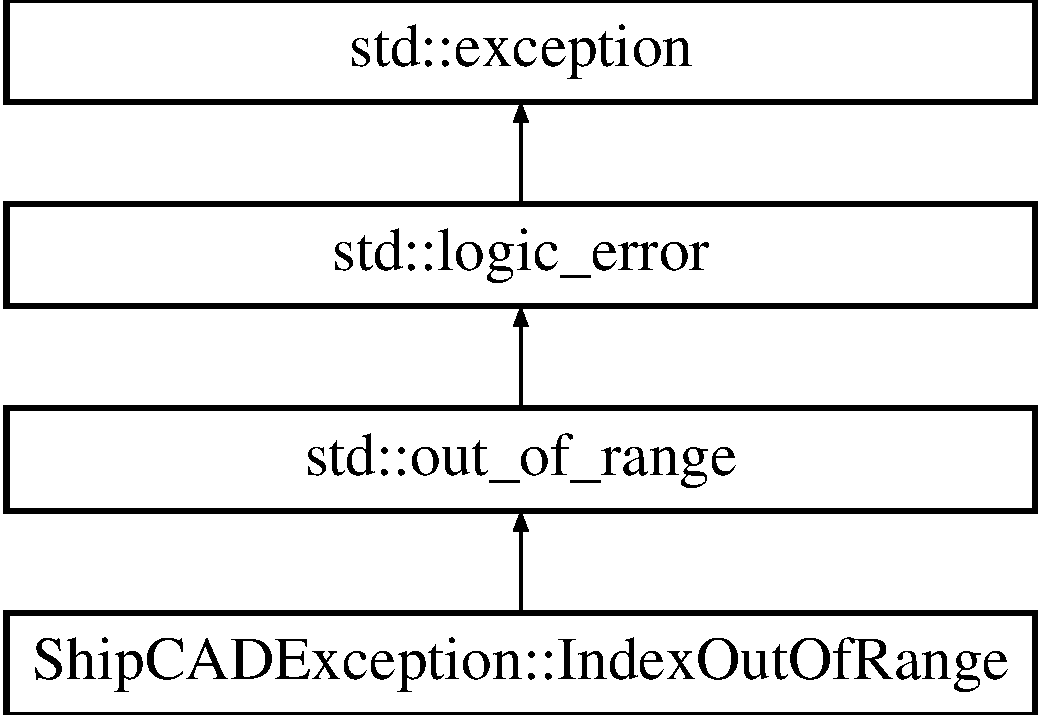
\includegraphics[height=4.000000cm]{classShipCADException_1_1IndexOutOfRange}
\end{center}
\end{figure}
\subsection*{Public Member Functions}
\begin{DoxyCompactItemize}
\item 
\hyperlink{classShipCADException_1_1IndexOutOfRange_a54f586b14f4cf32122861ceae07fce1f}{Index\-Out\-Of\-Range} (const std\-::string \&what\-\_\-arg)
\end{DoxyCompactItemize}


\subsection{Detailed Description}


Definition at line 50 of file exception.\-h.



\subsection{Constructor \& Destructor Documentation}
\hypertarget{classShipCADException_1_1IndexOutOfRange_a54f586b14f4cf32122861ceae07fce1f}{\index{Ship\-C\-A\-D\-Exception\-::\-Index\-Out\-Of\-Range@{Ship\-C\-A\-D\-Exception\-::\-Index\-Out\-Of\-Range}!Index\-Out\-Of\-Range@{Index\-Out\-Of\-Range}}
\index{Index\-Out\-Of\-Range@{Index\-Out\-Of\-Range}!ShipCADException::IndexOutOfRange@{Ship\-C\-A\-D\-Exception\-::\-Index\-Out\-Of\-Range}}
\subsubsection[{Index\-Out\-Of\-Range}]{\setlength{\rightskip}{0pt plus 5cm}Ship\-C\-A\-D\-Exception\-::\-Index\-Out\-Of\-Range\-::\-Index\-Out\-Of\-Range (
\begin{DoxyParamCaption}
\item[{const std\-::string \&}]{what\-\_\-arg}
\end{DoxyParamCaption}
)\hspace{0.3cm}{\ttfamily [inline]}}}\label{classShipCADException_1_1IndexOutOfRange_a54f586b14f4cf32122861ceae07fce1f}


Definition at line 53 of file exception.\-h.



The documentation for this class was generated from the following file\-:\begin{DoxyCompactItemize}
\item 
Ship\-C\-A\-Dlib/\hyperlink{exception_8h}{exception.\-h}\end{DoxyCompactItemize}

\hypertarget{classShipCADGeometry_1_1IntersectionData}{\section{Ship\-C\-A\-D\-Geometry\-:\-:Intersection\-Data Class Reference}
\label{classShipCADGeometry_1_1IntersectionData}\index{Ship\-C\-A\-D\-Geometry\-::\-Intersection\-Data@{Ship\-C\-A\-D\-Geometry\-::\-Intersection\-Data}}
}


{\ttfamily \#include $<$entity.\-h$>$}

Inheritance diagram for Ship\-C\-A\-D\-Geometry\-:\-:Intersection\-Data\-:\begin{figure}[H]
\begin{center}
\leavevmode
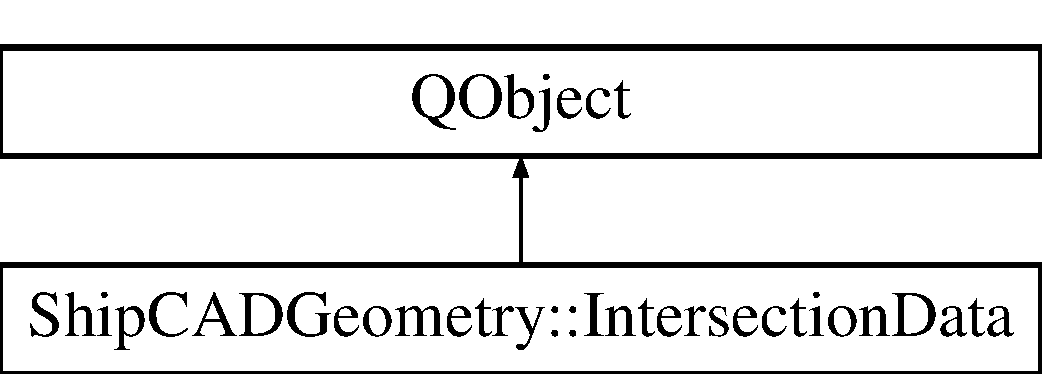
\includegraphics[height=2.000000cm]{classShipCADGeometry_1_1IntersectionData}
\end{center}
\end{figure}
\subsection*{Public Member Functions}
\begin{DoxyCompactItemize}
\item 
\hyperlink{classShipCADGeometry_1_1IntersectionData_a5c5deb18f585c790f4e3104769a51a13}{Intersection\-Data} ()
\item 
\hyperlink{classShipCADGeometry_1_1IntersectionData_a00da381c70a263a1da5a42adf3aa6e3d}{$\sim$\-Intersection\-Data} ()
\end{DoxyCompactItemize}
\subsection*{Public Attributes}
\begin{DoxyCompactItemize}
\item 
int \hyperlink{classShipCADGeometry_1_1IntersectionData_aff8a7bad6b802779c437df8b558be993}{number\-\_\-of\-\_\-intersections}
\item 
std\-::vector$<$ Q\-Vector3\-D $>$ \hyperlink{classShipCADGeometry_1_1IntersectionData_a7e38232a1c2af3ab1abff06ea87e9e8e}{points}
\item 
std\-::vector$<$ float $>$ \hyperlink{classShipCADGeometry_1_1IntersectionData_ac67f35f563f7c8f4dc7b1096e3ca8439}{parameters}
\end{DoxyCompactItemize}


\subsection{Detailed Description}


Definition at line 47 of file entity.\-h.



\subsection{Constructor \& Destructor Documentation}
\hypertarget{classShipCADGeometry_1_1IntersectionData_a5c5deb18f585c790f4e3104769a51a13}{\index{Ship\-C\-A\-D\-Geometry\-::\-Intersection\-Data@{Ship\-C\-A\-D\-Geometry\-::\-Intersection\-Data}!Intersection\-Data@{Intersection\-Data}}
\index{Intersection\-Data@{Intersection\-Data}!ShipCADGeometry::IntersectionData@{Ship\-C\-A\-D\-Geometry\-::\-Intersection\-Data}}
\subsubsection[{Intersection\-Data}]{\setlength{\rightskip}{0pt plus 5cm}Ship\-C\-A\-D\-Geometry\-::\-Intersection\-Data\-::\-Intersection\-Data (
\begin{DoxyParamCaption}
{}
\end{DoxyParamCaption}
)\hspace{0.3cm}{\ttfamily [inline]}, {\ttfamily [explicit]}}}\label{classShipCADGeometry_1_1IntersectionData_a5c5deb18f585c790f4e3104769a51a13}


Definition at line 52 of file entity.\-h.

\hypertarget{classShipCADGeometry_1_1IntersectionData_a00da381c70a263a1da5a42adf3aa6e3d}{\index{Ship\-C\-A\-D\-Geometry\-::\-Intersection\-Data@{Ship\-C\-A\-D\-Geometry\-::\-Intersection\-Data}!$\sim$\-Intersection\-Data@{$\sim$\-Intersection\-Data}}
\index{$\sim$\-Intersection\-Data@{$\sim$\-Intersection\-Data}!ShipCADGeometry::IntersectionData@{Ship\-C\-A\-D\-Geometry\-::\-Intersection\-Data}}
\subsubsection[{$\sim$\-Intersection\-Data}]{\setlength{\rightskip}{0pt plus 5cm}Ship\-C\-A\-D\-Geometry\-::\-Intersection\-Data\-::$\sim$\-Intersection\-Data (
\begin{DoxyParamCaption}
{}
\end{DoxyParamCaption}
)\hspace{0.3cm}{\ttfamily [inline]}}}\label{classShipCADGeometry_1_1IntersectionData_a00da381c70a263a1da5a42adf3aa6e3d}


Definition at line 53 of file entity.\-h.



\subsection{Member Data Documentation}
\hypertarget{classShipCADGeometry_1_1IntersectionData_aff8a7bad6b802779c437df8b558be993}{\index{Ship\-C\-A\-D\-Geometry\-::\-Intersection\-Data@{Ship\-C\-A\-D\-Geometry\-::\-Intersection\-Data}!number\-\_\-of\-\_\-intersections@{number\-\_\-of\-\_\-intersections}}
\index{number\-\_\-of\-\_\-intersections@{number\-\_\-of\-\_\-intersections}!ShipCADGeometry::IntersectionData@{Ship\-C\-A\-D\-Geometry\-::\-Intersection\-Data}}
\subsubsection[{number\-\_\-of\-\_\-intersections}]{\setlength{\rightskip}{0pt plus 5cm}int Ship\-C\-A\-D\-Geometry\-::\-Intersection\-Data\-::number\-\_\-of\-\_\-intersections}}\label{classShipCADGeometry_1_1IntersectionData_aff8a7bad6b802779c437df8b558be993}


Definition at line 55 of file entity.\-h.

\hypertarget{classShipCADGeometry_1_1IntersectionData_ac67f35f563f7c8f4dc7b1096e3ca8439}{\index{Ship\-C\-A\-D\-Geometry\-::\-Intersection\-Data@{Ship\-C\-A\-D\-Geometry\-::\-Intersection\-Data}!parameters@{parameters}}
\index{parameters@{parameters}!ShipCADGeometry::IntersectionData@{Ship\-C\-A\-D\-Geometry\-::\-Intersection\-Data}}
\subsubsection[{parameters}]{\setlength{\rightskip}{0pt plus 5cm}std\-::vector$<$float$>$ Ship\-C\-A\-D\-Geometry\-::\-Intersection\-Data\-::parameters}}\label{classShipCADGeometry_1_1IntersectionData_ac67f35f563f7c8f4dc7b1096e3ca8439}


Definition at line 57 of file entity.\-h.

\hypertarget{classShipCADGeometry_1_1IntersectionData_a7e38232a1c2af3ab1abff06ea87e9e8e}{\index{Ship\-C\-A\-D\-Geometry\-::\-Intersection\-Data@{Ship\-C\-A\-D\-Geometry\-::\-Intersection\-Data}!points@{points}}
\index{points@{points}!ShipCADGeometry::IntersectionData@{Ship\-C\-A\-D\-Geometry\-::\-Intersection\-Data}}
\subsubsection[{points}]{\setlength{\rightskip}{0pt plus 5cm}std\-::vector$<$Q\-Vector3\-D$>$ Ship\-C\-A\-D\-Geometry\-::\-Intersection\-Data\-::points}}\label{classShipCADGeometry_1_1IntersectionData_a7e38232a1c2af3ab1abff06ea87e9e8e}


Definition at line 56 of file entity.\-h.



The documentation for this class was generated from the following file\-:\begin{DoxyCompactItemize}
\item 
Ship\-C\-A\-Dlib/\hyperlink{entity_8h}{entity.\-h}\end{DoxyCompactItemize}

\hypertarget{structShipCADGeometry_1_1LayerProperties}{\section{Ship\-C\-A\-D\-Geometry\-:\-:Layer\-Properties Struct Reference}
\label{structShipCADGeometry_1_1LayerProperties}\index{Ship\-C\-A\-D\-Geometry\-::\-Layer\-Properties@{Ship\-C\-A\-D\-Geometry\-::\-Layer\-Properties}}
}


{\ttfamily \#include $<$subdivlayer.\-h$>$}

\subsection*{Public Attributes}
\begin{DoxyCompactItemize}
\item 
float \hyperlink{structShipCADGeometry_1_1LayerProperties_aec92af25292b8dcfa668155a3e051dfb}{surface\-\_\-area}
\item 
float \hyperlink{structShipCADGeometry_1_1LayerProperties_a6905a3f5c097cc4f251455a6267c9db9}{weight}
\item 
Q\-Vector3\-D \hyperlink{structShipCADGeometry_1_1LayerProperties_aa30ff3a9afe247ba04327d79f4f398c4}{surface\-\_\-center\-\_\-of\-\_\-gravity}
\end{DoxyCompactItemize}


\subsection{Detailed Description}


Definition at line 52 of file subdivlayer.\-h.



\subsection{Member Data Documentation}
\hypertarget{structShipCADGeometry_1_1LayerProperties_aec92af25292b8dcfa668155a3e051dfb}{\index{Ship\-C\-A\-D\-Geometry\-::\-Layer\-Properties@{Ship\-C\-A\-D\-Geometry\-::\-Layer\-Properties}!surface\-\_\-area@{surface\-\_\-area}}
\index{surface\-\_\-area@{surface\-\_\-area}!ShipCADGeometry::LayerProperties@{Ship\-C\-A\-D\-Geometry\-::\-Layer\-Properties}}
\subsubsection[{surface\-\_\-area}]{\setlength{\rightskip}{0pt plus 5cm}float Ship\-C\-A\-D\-Geometry\-::\-Layer\-Properties\-::surface\-\_\-area}}\label{structShipCADGeometry_1_1LayerProperties_aec92af25292b8dcfa668155a3e051dfb}


Definition at line 54 of file subdivlayer.\-h.

\hypertarget{structShipCADGeometry_1_1LayerProperties_aa30ff3a9afe247ba04327d79f4f398c4}{\index{Ship\-C\-A\-D\-Geometry\-::\-Layer\-Properties@{Ship\-C\-A\-D\-Geometry\-::\-Layer\-Properties}!surface\-\_\-center\-\_\-of\-\_\-gravity@{surface\-\_\-center\-\_\-of\-\_\-gravity}}
\index{surface\-\_\-center\-\_\-of\-\_\-gravity@{surface\-\_\-center\-\_\-of\-\_\-gravity}!ShipCADGeometry::LayerProperties@{Ship\-C\-A\-D\-Geometry\-::\-Layer\-Properties}}
\subsubsection[{surface\-\_\-center\-\_\-of\-\_\-gravity}]{\setlength{\rightskip}{0pt plus 5cm}Q\-Vector3\-D Ship\-C\-A\-D\-Geometry\-::\-Layer\-Properties\-::surface\-\_\-center\-\_\-of\-\_\-gravity}}\label{structShipCADGeometry_1_1LayerProperties_aa30ff3a9afe247ba04327d79f4f398c4}


Definition at line 56 of file subdivlayer.\-h.

\hypertarget{structShipCADGeometry_1_1LayerProperties_a6905a3f5c097cc4f251455a6267c9db9}{\index{Ship\-C\-A\-D\-Geometry\-::\-Layer\-Properties@{Ship\-C\-A\-D\-Geometry\-::\-Layer\-Properties}!weight@{weight}}
\index{weight@{weight}!ShipCADGeometry::LayerProperties@{Ship\-C\-A\-D\-Geometry\-::\-Layer\-Properties}}
\subsubsection[{weight}]{\setlength{\rightskip}{0pt plus 5cm}float Ship\-C\-A\-D\-Geometry\-::\-Layer\-Properties\-::weight}}\label{structShipCADGeometry_1_1LayerProperties_a6905a3f5c097cc4f251455a6267c9db9}


Definition at line 55 of file subdivlayer.\-h.



The documentation for this struct was generated from the following file\-:\begin{DoxyCompactItemize}
\item 
Ship\-C\-A\-Dlib/\hyperlink{subdivlayer_8h}{subdivlayer.\-h}\end{DoxyCompactItemize}

\hypertarget{classShipCADGeometry_1_1LineShader}{\section{Ship\-C\-A\-D\-Geometry\-:\-:Line\-Shader Class Reference}
\label{classShipCADGeometry_1_1LineShader}\index{Ship\-C\-A\-D\-Geometry\-::\-Line\-Shader@{Ship\-C\-A\-D\-Geometry\-::\-Line\-Shader}}
}


{\ttfamily \#include $<$shader.\-h$>$}

Inheritance diagram for Ship\-C\-A\-D\-Geometry\-:\-:Line\-Shader\-:\begin{figure}[H]
\begin{center}
\leavevmode
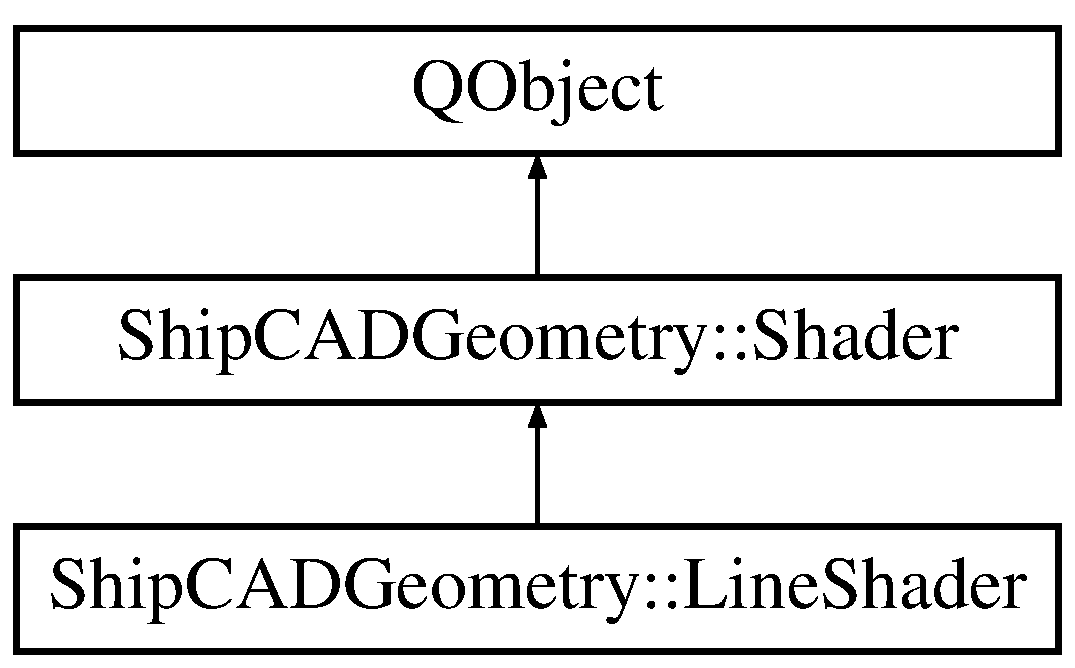
\includegraphics[height=3.000000cm]{classShipCADGeometry_1_1LineShader}
\end{center}
\end{figure}
\subsection*{Public Member Functions}
\begin{DoxyCompactItemize}
\item 
\hyperlink{classShipCADGeometry_1_1LineShader_ae06ecf68dfc054511db3937893850d2f}{Line\-Shader} (\hyperlink{classShipCADGeometry_1_1Viewport}{Viewport} $\ast$vp)
\item 
virtual \hyperlink{classShipCADGeometry_1_1LineShader_a0bbbe35354d12edfff172d35c8023163}{$\sim$\-Line\-Shader} ()
\item 
void \hyperlink{classShipCADGeometry_1_1LineShader_aaa105117e559ec413a733e14dc638b5a}{render\-Points} (Q\-Vector$<$ Q\-Vector3\-D $>$ \&points, Q\-Color color)
\item 
void \hyperlink{classShipCADGeometry_1_1LineShader_a3d30bda1883e0eda65ea23c4da76f610}{render\-Lines} (Q\-Vector$<$ Q\-Vector3\-D $>$ \&vertices, Q\-Color line\-Color)
\end{DoxyCompactItemize}
\subsection*{Additional Inherited Members}


\subsection{Detailed Description}


Definition at line 77 of file shader.\-h.



\subsection{Constructor \& Destructor Documentation}
\hypertarget{classShipCADGeometry_1_1LineShader_ae06ecf68dfc054511db3937893850d2f}{\index{Ship\-C\-A\-D\-Geometry\-::\-Line\-Shader@{Ship\-C\-A\-D\-Geometry\-::\-Line\-Shader}!Line\-Shader@{Line\-Shader}}
\index{Line\-Shader@{Line\-Shader}!ShipCADGeometry::LineShader@{Ship\-C\-A\-D\-Geometry\-::\-Line\-Shader}}
\subsubsection[{Line\-Shader}]{\setlength{\rightskip}{0pt plus 5cm}Line\-Shader\-::\-Line\-Shader (
\begin{DoxyParamCaption}
\item[{{\bf Viewport} $\ast$}]{vp}
\end{DoxyParamCaption}
)\hspace{0.3cm}{\ttfamily [explicit]}}}\label{classShipCADGeometry_1_1LineShader_ae06ecf68dfc054511db3937893850d2f}


Definition at line 110 of file shader.\-cpp.

\hypertarget{classShipCADGeometry_1_1LineShader_a0bbbe35354d12edfff172d35c8023163}{\index{Ship\-C\-A\-D\-Geometry\-::\-Line\-Shader@{Ship\-C\-A\-D\-Geometry\-::\-Line\-Shader}!$\sim$\-Line\-Shader@{$\sim$\-Line\-Shader}}
\index{$\sim$\-Line\-Shader@{$\sim$\-Line\-Shader}!ShipCADGeometry::LineShader@{Ship\-C\-A\-D\-Geometry\-::\-Line\-Shader}}
\subsubsection[{$\sim$\-Line\-Shader}]{\setlength{\rightskip}{0pt plus 5cm}virtual Ship\-C\-A\-D\-Geometry\-::\-Line\-Shader\-::$\sim$\-Line\-Shader (
\begin{DoxyParamCaption}
{}
\end{DoxyParamCaption}
)\hspace{0.3cm}{\ttfamily [inline]}, {\ttfamily [virtual]}}}\label{classShipCADGeometry_1_1LineShader_a0bbbe35354d12edfff172d35c8023163}


Definition at line 84 of file shader.\-h.



\subsection{Member Function Documentation}
\hypertarget{classShipCADGeometry_1_1LineShader_a3d30bda1883e0eda65ea23c4da76f610}{\index{Ship\-C\-A\-D\-Geometry\-::\-Line\-Shader@{Ship\-C\-A\-D\-Geometry\-::\-Line\-Shader}!render\-Lines@{render\-Lines}}
\index{render\-Lines@{render\-Lines}!ShipCADGeometry::LineShader@{Ship\-C\-A\-D\-Geometry\-::\-Line\-Shader}}
\subsubsection[{render\-Lines}]{\setlength{\rightskip}{0pt plus 5cm}void Line\-Shader\-::render\-Lines (
\begin{DoxyParamCaption}
\item[{Q\-Vector$<$ Q\-Vector3\-D $>$ \&}]{vertices, }
\item[{Q\-Color}]{line\-Color}
\end{DoxyParamCaption}
)}}\label{classShipCADGeometry_1_1LineShader_a3d30bda1883e0eda65ea23c4da76f610}


Definition at line 136 of file shader.\-cpp.

\hypertarget{classShipCADGeometry_1_1LineShader_aaa105117e559ec413a733e14dc638b5a}{\index{Ship\-C\-A\-D\-Geometry\-::\-Line\-Shader@{Ship\-C\-A\-D\-Geometry\-::\-Line\-Shader}!render\-Points@{render\-Points}}
\index{render\-Points@{render\-Points}!ShipCADGeometry::LineShader@{Ship\-C\-A\-D\-Geometry\-::\-Line\-Shader}}
\subsubsection[{render\-Points}]{\setlength{\rightskip}{0pt plus 5cm}void Line\-Shader\-::render\-Points (
\begin{DoxyParamCaption}
\item[{Q\-Vector$<$ Q\-Vector3\-D $>$ \&}]{points, }
\item[{Q\-Color}]{color}
\end{DoxyParamCaption}
)}}\label{classShipCADGeometry_1_1LineShader_aaa105117e559ec413a733e14dc638b5a}


Definition at line 120 of file shader.\-cpp.



The documentation for this class was generated from the following files\-:\begin{DoxyCompactItemize}
\item 
Ship\-C\-A\-Dlib/\hyperlink{shader_8h}{shader.\-h}\item 
Ship\-C\-A\-Dlib/\hyperlink{shader_8cpp}{shader.\-cpp}\end{DoxyCompactItemize}

\hypertarget{classShipCADException_1_1ListIndexOutOfBounds}{\section{Ship\-C\-A\-D\-Exception\-:\-:List\-Index\-Out\-Of\-Bounds Class Reference}
\label{classShipCADException_1_1ListIndexOutOfBounds}\index{Ship\-C\-A\-D\-Exception\-::\-List\-Index\-Out\-Of\-Bounds@{Ship\-C\-A\-D\-Exception\-::\-List\-Index\-Out\-Of\-Bounds}}
}


{\ttfamily \#include $<$exception.\-h$>$}

Inheritance diagram for Ship\-C\-A\-D\-Exception\-:\-:List\-Index\-Out\-Of\-Bounds\-:\begin{figure}[H]
\begin{center}
\leavevmode
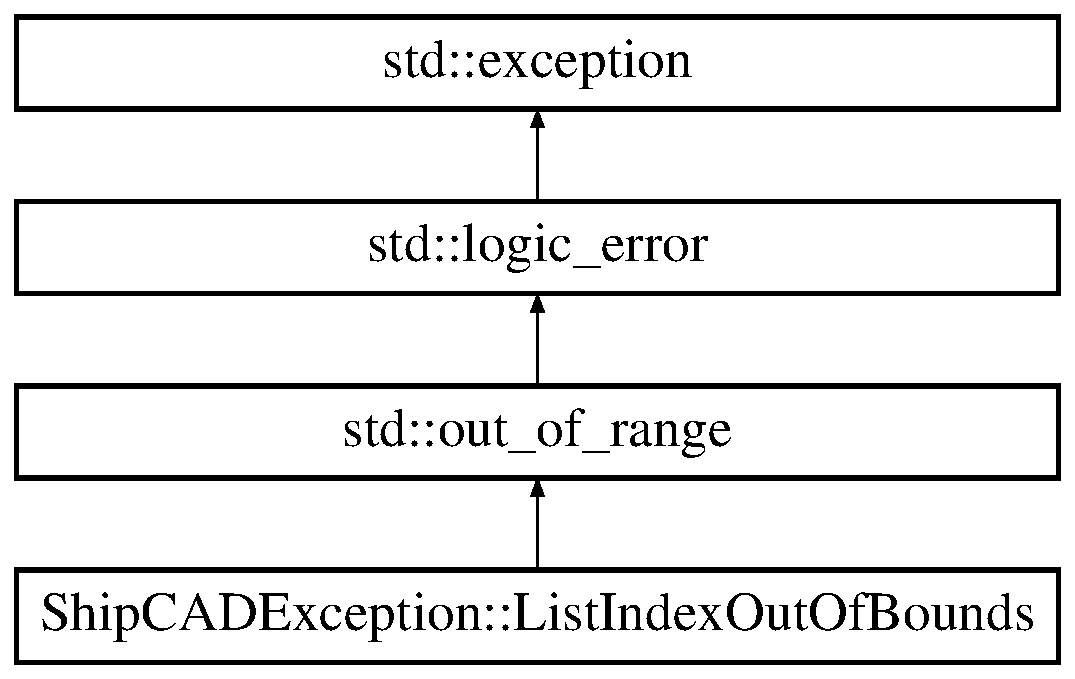
\includegraphics[height=4.000000cm]{classShipCADException_1_1ListIndexOutOfBounds}
\end{center}
\end{figure}
\subsection*{Public Member Functions}
\begin{DoxyCompactItemize}
\item 
\hyperlink{classShipCADException_1_1ListIndexOutOfBounds_a156855cdf77b85b6b223cbffced87429}{List\-Index\-Out\-Of\-Bounds} (const std\-::string \&what\-\_\-arg)
\end{DoxyCompactItemize}


\subsection{Detailed Description}


Definition at line 38 of file exception.\-h.



\subsection{Constructor \& Destructor Documentation}
\hypertarget{classShipCADException_1_1ListIndexOutOfBounds_a156855cdf77b85b6b223cbffced87429}{\index{Ship\-C\-A\-D\-Exception\-::\-List\-Index\-Out\-Of\-Bounds@{Ship\-C\-A\-D\-Exception\-::\-List\-Index\-Out\-Of\-Bounds}!List\-Index\-Out\-Of\-Bounds@{List\-Index\-Out\-Of\-Bounds}}
\index{List\-Index\-Out\-Of\-Bounds@{List\-Index\-Out\-Of\-Bounds}!ShipCADException::ListIndexOutOfBounds@{Ship\-C\-A\-D\-Exception\-::\-List\-Index\-Out\-Of\-Bounds}}
\subsubsection[{List\-Index\-Out\-Of\-Bounds}]{\setlength{\rightskip}{0pt plus 5cm}Ship\-C\-A\-D\-Exception\-::\-List\-Index\-Out\-Of\-Bounds\-::\-List\-Index\-Out\-Of\-Bounds (
\begin{DoxyParamCaption}
\item[{const std\-::string \&}]{what\-\_\-arg}
\end{DoxyParamCaption}
)\hspace{0.3cm}{\ttfamily [inline]}}}\label{classShipCADException_1_1ListIndexOutOfBounds_a156855cdf77b85b6b223cbffced87429}


Definition at line 41 of file exception.\-h.



The documentation for this class was generated from the following file\-:\begin{DoxyCompactItemize}
\item 
Ship\-C\-A\-Dlib/\hyperlink{exception_8h}{exception.\-h}\end{DoxyCompactItemize}

\hypertarget{classMainWindow}{\section{Main\-Window Class Reference}
\label{classMainWindow}\index{Main\-Window@{Main\-Window}}
}


{\ttfamily \#include $<$mainwindow.\-h$>$}

Inheritance diagram for Main\-Window\-:\begin{figure}[H]
\begin{center}
\leavevmode
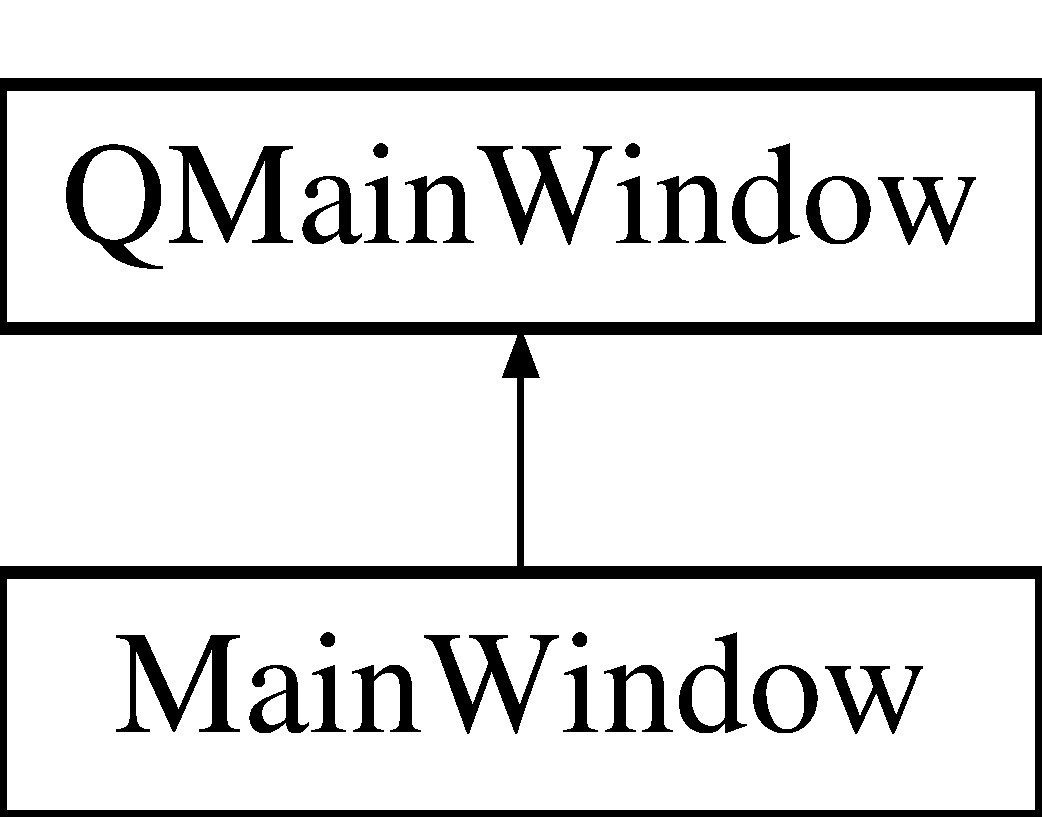
\includegraphics[height=2.000000cm]{classMainWindow}
\end{center}
\end{figure}
\subsection*{Public Slots}
\begin{DoxyCompactItemize}
\item 
void \hyperlink{classMainWindow_a288b768c3c21a9171bdc56fe845ece8b}{open\-File} ()
\end{DoxyCompactItemize}
\subsection*{Public Member Functions}
\begin{DoxyCompactItemize}
\item 
\hyperlink{classMainWindow_a8b244be8b7b7db1b08de2a2acb9409db}{Main\-Window} (Q\-Widget $\ast$parent=0)
\item 
\hyperlink{classMainWindow_ae98d00a93bc118200eeef9f9bba1dba7}{$\sim$\-Main\-Window} ()
\item 
void \hyperlink{classMainWindow_ae53d70703200d86162a68a9a8ba593ee}{set\-Animating} (bool animating)
\item 
void \hyperlink{classMainWindow_a09cb0428e2c3a4226c04eafff3904f5d}{set\-Surface} (\hyperlink{classShipCAD_1_1SubdivisionSurface}{Ship\-C\-A\-D\-::\-Subdivision\-Surface} $\ast$surface)
\end{DoxyCompactItemize}
\subsection*{Protected Slots}
\begin{DoxyCompactItemize}
\item 
void \hyperlink{classMainWindow_a8690702fe505fb6786ae98f9cad71118}{wire\-Frame} ()
\item 
void \hyperlink{classMainWindow_ad2040b40c2d18b4dea61d33699ae0a90}{shade} ()
\item 
void \hyperlink{classMainWindow_af7f1931b45432a43105345f806097501}{shade\-Curvature} ()
\item 
void \hyperlink{classMainWindow_a7827c32592a7991f37e87f2ba94b3ccd}{shade\-Developable} ()
\item 
void \hyperlink{classMainWindow_afc072912649b8cc513963db3b2f05283}{shade\-Zebra} ()
\item 
void \hyperlink{classMainWindow_a93b8868bdce207842de4747008f5e03e}{show\-Control\-Net} (bool val)
\item 
void \hyperlink{classMainWindow_aa0401a2a6241ff56390b1825f4e0e508}{show\-Interior\-Edges} (bool val)
\item 
void \hyperlink{classMainWindow_ac7ec359ed2a0f3c66ba5d2a788613832}{show\-Control\-Curves} (bool val)
\item 
void \hyperlink{classMainWindow_a65462f395b206a9a680a5521082b6344}{show\-Curvature} (bool val)
\item 
void \hyperlink{classMainWindow_a8edd7fa619d2ed66b94f6a498f5af59c}{show\-Normals} (bool val)
\item 
void \hyperlink{classMainWindow_afb7953f1fdcb7c5a77efa6fb4d2c3cd5}{draw\-Mirror} (bool val)
\item 
void \hyperlink{classMainWindow_adecb2e29c0d3df68517a570dc9e352bd}{shade\-Underwater} (bool val)
\item 
void \hyperlink{classMainWindow_a4a399825baba544bf4850e06e5e1fa94}{animation\-Timeout} ()
\end{DoxyCompactItemize}


\subsection{Detailed Description}


Definition at line 45 of file mainwindow.\-h.



\subsection{Constructor \& Destructor Documentation}
\hypertarget{classMainWindow_a8b244be8b7b7db1b08de2a2acb9409db}{\index{Main\-Window@{Main\-Window}!Main\-Window@{Main\-Window}}
\index{Main\-Window@{Main\-Window}!MainWindow@{Main\-Window}}
\subsubsection[{Main\-Window}]{\setlength{\rightskip}{0pt plus 5cm}Main\-Window\-::\-Main\-Window (
\begin{DoxyParamCaption}
\item[{Q\-Widget $\ast$}]{parent = {\ttfamily 0}}
\end{DoxyParamCaption}
)\hspace{0.3cm}{\ttfamily [explicit]}}}\label{classMainWindow_a8b244be8b7b7db1b08de2a2acb9409db}


Definition at line 48 of file mainwindow.\-cpp.

\hypertarget{classMainWindow_ae98d00a93bc118200eeef9f9bba1dba7}{\index{Main\-Window@{Main\-Window}!$\sim$\-Main\-Window@{$\sim$\-Main\-Window}}
\index{$\sim$\-Main\-Window@{$\sim$\-Main\-Window}!MainWindow@{Main\-Window}}
\subsubsection[{$\sim$\-Main\-Window}]{\setlength{\rightskip}{0pt plus 5cm}Main\-Window\-::$\sim$\-Main\-Window (
\begin{DoxyParamCaption}
{}
\end{DoxyParamCaption}
)}}\label{classMainWindow_ae98d00a93bc118200eeef9f9bba1dba7}


Definition at line 159 of file mainwindow.\-cpp.



\subsection{Member Function Documentation}
\hypertarget{classMainWindow_a4a399825baba544bf4850e06e5e1fa94}{\index{Main\-Window@{Main\-Window}!animation\-Timeout@{animation\-Timeout}}
\index{animation\-Timeout@{animation\-Timeout}!MainWindow@{Main\-Window}}
\subsubsection[{animation\-Timeout}]{\setlength{\rightskip}{0pt plus 5cm}void Main\-Window\-::animation\-Timeout (
\begin{DoxyParamCaption}
{}
\end{DoxyParamCaption}
)\hspace{0.3cm}{\ttfamily [protected]}, {\ttfamily [slot]}}}\label{classMainWindow_a4a399825baba544bf4850e06e5e1fa94}


Definition at line 186 of file mainwindow.\-cpp.

\hypertarget{classMainWindow_afb7953f1fdcb7c5a77efa6fb4d2c3cd5}{\index{Main\-Window@{Main\-Window}!draw\-Mirror@{draw\-Mirror}}
\index{draw\-Mirror@{draw\-Mirror}!MainWindow@{Main\-Window}}
\subsubsection[{draw\-Mirror}]{\setlength{\rightskip}{0pt plus 5cm}void Main\-Window\-::draw\-Mirror (
\begin{DoxyParamCaption}
\item[{bool}]{val}
\end{DoxyParamCaption}
)\hspace{0.3cm}{\ttfamily [protected]}, {\ttfamily [slot]}}}\label{classMainWindow_afb7953f1fdcb7c5a77efa6fb4d2c3cd5}


Definition at line 360 of file mainwindow.\-cpp.

\hypertarget{classMainWindow_a288b768c3c21a9171bdc56fe845ece8b}{\index{Main\-Window@{Main\-Window}!open\-File@{open\-File}}
\index{open\-File@{open\-File}!MainWindow@{Main\-Window}}
\subsubsection[{open\-File}]{\setlength{\rightskip}{0pt plus 5cm}void Main\-Window\-::open\-File (
\begin{DoxyParamCaption}
{}
\end{DoxyParamCaption}
)\hspace{0.3cm}{\ttfamily [slot]}}}\label{classMainWindow_a288b768c3c21a9171bdc56fe845ece8b}


Definition at line 211 of file mainwindow.\-cpp.

\hypertarget{classMainWindow_ae53d70703200d86162a68a9a8ba593ee}{\index{Main\-Window@{Main\-Window}!set\-Animating@{set\-Animating}}
\index{set\-Animating@{set\-Animating}!MainWindow@{Main\-Window}}
\subsubsection[{set\-Animating}]{\setlength{\rightskip}{0pt plus 5cm}void Main\-Window\-::set\-Animating (
\begin{DoxyParamCaption}
\item[{bool}]{animating}
\end{DoxyParamCaption}
)}}\label{classMainWindow_ae53d70703200d86162a68a9a8ba593ee}


Definition at line 167 of file mainwindow.\-cpp.

\hypertarget{classMainWindow_a09cb0428e2c3a4226c04eafff3904f5d}{\index{Main\-Window@{Main\-Window}!set\-Surface@{set\-Surface}}
\index{set\-Surface@{set\-Surface}!MainWindow@{Main\-Window}}
\subsubsection[{set\-Surface}]{\setlength{\rightskip}{0pt plus 5cm}void Main\-Window\-::set\-Surface (
\begin{DoxyParamCaption}
\item[{{\bf Ship\-C\-A\-D\-::\-Subdivision\-Surface} $\ast$}]{surface}
\end{DoxyParamCaption}
)}}\label{classMainWindow_a09cb0428e2c3a4226c04eafff3904f5d}


Definition at line 250 of file mainwindow.\-cpp.

\hypertarget{classMainWindow_ad2040b40c2d18b4dea61d33699ae0a90}{\index{Main\-Window@{Main\-Window}!shade@{shade}}
\index{shade@{shade}!MainWindow@{Main\-Window}}
\subsubsection[{shade}]{\setlength{\rightskip}{0pt plus 5cm}void Main\-Window\-::shade (
\begin{DoxyParamCaption}
{}
\end{DoxyParamCaption}
)\hspace{0.3cm}{\ttfamily [protected]}, {\ttfamily [slot]}}}\label{classMainWindow_ad2040b40c2d18b4dea61d33699ae0a90}


Definition at line 273 of file mainwindow.\-cpp.

\hypertarget{classMainWindow_af7f1931b45432a43105345f806097501}{\index{Main\-Window@{Main\-Window}!shade\-Curvature@{shade\-Curvature}}
\index{shade\-Curvature@{shade\-Curvature}!MainWindow@{Main\-Window}}
\subsubsection[{shade\-Curvature}]{\setlength{\rightskip}{0pt plus 5cm}void Main\-Window\-::shade\-Curvature (
\begin{DoxyParamCaption}
{}
\end{DoxyParamCaption}
)\hspace{0.3cm}{\ttfamily [protected]}, {\ttfamily [slot]}}}\label{classMainWindow_af7f1931b45432a43105345f806097501}


Definition at line 281 of file mainwindow.\-cpp.

\hypertarget{classMainWindow_a7827c32592a7991f37e87f2ba94b3ccd}{\index{Main\-Window@{Main\-Window}!shade\-Developable@{shade\-Developable}}
\index{shade\-Developable@{shade\-Developable}!MainWindow@{Main\-Window}}
\subsubsection[{shade\-Developable}]{\setlength{\rightskip}{0pt plus 5cm}void Main\-Window\-::shade\-Developable (
\begin{DoxyParamCaption}
{}
\end{DoxyParamCaption}
)\hspace{0.3cm}{\ttfamily [protected]}, {\ttfamily [slot]}}}\label{classMainWindow_a7827c32592a7991f37e87f2ba94b3ccd}


Definition at line 289 of file mainwindow.\-cpp.

\hypertarget{classMainWindow_adecb2e29c0d3df68517a570dc9e352bd}{\index{Main\-Window@{Main\-Window}!shade\-Underwater@{shade\-Underwater}}
\index{shade\-Underwater@{shade\-Underwater}!MainWindow@{Main\-Window}}
\subsubsection[{shade\-Underwater}]{\setlength{\rightskip}{0pt plus 5cm}void Main\-Window\-::shade\-Underwater (
\begin{DoxyParamCaption}
\item[{bool}]{val}
\end{DoxyParamCaption}
)\hspace{0.3cm}{\ttfamily [protected]}, {\ttfamily [slot]}}}\label{classMainWindow_adecb2e29c0d3df68517a570dc9e352bd}


Definition at line 371 of file mainwindow.\-cpp.

\hypertarget{classMainWindow_afc072912649b8cc513963db3b2f05283}{\index{Main\-Window@{Main\-Window}!shade\-Zebra@{shade\-Zebra}}
\index{shade\-Zebra@{shade\-Zebra}!MainWindow@{Main\-Window}}
\subsubsection[{shade\-Zebra}]{\setlength{\rightskip}{0pt plus 5cm}void Main\-Window\-::shade\-Zebra (
\begin{DoxyParamCaption}
{}
\end{DoxyParamCaption}
)\hspace{0.3cm}{\ttfamily [protected]}, {\ttfamily [slot]}}}\label{classMainWindow_afc072912649b8cc513963db3b2f05283}


Definition at line 297 of file mainwindow.\-cpp.

\hypertarget{classMainWindow_ac7ec359ed2a0f3c66ba5d2a788613832}{\index{Main\-Window@{Main\-Window}!show\-Control\-Curves@{show\-Control\-Curves}}
\index{show\-Control\-Curves@{show\-Control\-Curves}!MainWindow@{Main\-Window}}
\subsubsection[{show\-Control\-Curves}]{\setlength{\rightskip}{0pt plus 5cm}void Main\-Window\-::show\-Control\-Curves (
\begin{DoxyParamCaption}
\item[{bool}]{val}
\end{DoxyParamCaption}
)\hspace{0.3cm}{\ttfamily [protected]}, {\ttfamily [slot]}}}\label{classMainWindow_ac7ec359ed2a0f3c66ba5d2a788613832}


Definition at line 327 of file mainwindow.\-cpp.

\hypertarget{classMainWindow_a93b8868bdce207842de4747008f5e03e}{\index{Main\-Window@{Main\-Window}!show\-Control\-Net@{show\-Control\-Net}}
\index{show\-Control\-Net@{show\-Control\-Net}!MainWindow@{Main\-Window}}
\subsubsection[{show\-Control\-Net}]{\setlength{\rightskip}{0pt plus 5cm}void Main\-Window\-::show\-Control\-Net (
\begin{DoxyParamCaption}
\item[{bool}]{val}
\end{DoxyParamCaption}
)\hspace{0.3cm}{\ttfamily [protected]}, {\ttfamily [slot]}}}\label{classMainWindow_a93b8868bdce207842de4747008f5e03e}


Definition at line 305 of file mainwindow.\-cpp.

\hypertarget{classMainWindow_a65462f395b206a9a680a5521082b6344}{\index{Main\-Window@{Main\-Window}!show\-Curvature@{show\-Curvature}}
\index{show\-Curvature@{show\-Curvature}!MainWindow@{Main\-Window}}
\subsubsection[{show\-Curvature}]{\setlength{\rightskip}{0pt plus 5cm}void Main\-Window\-::show\-Curvature (
\begin{DoxyParamCaption}
\item[{bool}]{val}
\end{DoxyParamCaption}
)\hspace{0.3cm}{\ttfamily [protected]}, {\ttfamily [slot]}}}\label{classMainWindow_a65462f395b206a9a680a5521082b6344}


Definition at line 338 of file mainwindow.\-cpp.

\hypertarget{classMainWindow_aa0401a2a6241ff56390b1825f4e0e508}{\index{Main\-Window@{Main\-Window}!show\-Interior\-Edges@{show\-Interior\-Edges}}
\index{show\-Interior\-Edges@{show\-Interior\-Edges}!MainWindow@{Main\-Window}}
\subsubsection[{show\-Interior\-Edges}]{\setlength{\rightskip}{0pt plus 5cm}void Main\-Window\-::show\-Interior\-Edges (
\begin{DoxyParamCaption}
\item[{bool}]{val}
\end{DoxyParamCaption}
)\hspace{0.3cm}{\ttfamily [protected]}, {\ttfamily [slot]}}}\label{classMainWindow_aa0401a2a6241ff56390b1825f4e0e508}


Definition at line 316 of file mainwindow.\-cpp.

\hypertarget{classMainWindow_a8edd7fa619d2ed66b94f6a498f5af59c}{\index{Main\-Window@{Main\-Window}!show\-Normals@{show\-Normals}}
\index{show\-Normals@{show\-Normals}!MainWindow@{Main\-Window}}
\subsubsection[{show\-Normals}]{\setlength{\rightskip}{0pt plus 5cm}void Main\-Window\-::show\-Normals (
\begin{DoxyParamCaption}
\item[{bool}]{val}
\end{DoxyParamCaption}
)\hspace{0.3cm}{\ttfamily [protected]}, {\ttfamily [slot]}}}\label{classMainWindow_a8edd7fa619d2ed66b94f6a498f5af59c}


Definition at line 349 of file mainwindow.\-cpp.

\hypertarget{classMainWindow_a8690702fe505fb6786ae98f9cad71118}{\index{Main\-Window@{Main\-Window}!wire\-Frame@{wire\-Frame}}
\index{wire\-Frame@{wire\-Frame}!MainWindow@{Main\-Window}}
\subsubsection[{wire\-Frame}]{\setlength{\rightskip}{0pt plus 5cm}void Main\-Window\-::wire\-Frame (
\begin{DoxyParamCaption}
{}
\end{DoxyParamCaption}
)\hspace{0.3cm}{\ttfamily [protected]}, {\ttfamily [slot]}}}\label{classMainWindow_a8690702fe505fb6786ae98f9cad71118}


Definition at line 265 of file mainwindow.\-cpp.



The documentation for this class was generated from the following files\-:\begin{DoxyCompactItemize}
\item 
Viewer/\hyperlink{mainwindow_8h}{mainwindow.\-h}\item 
Viewer/\hyperlink{mainwindow_8cpp}{mainwindow.\-cpp}\end{DoxyCompactItemize}

\hypertarget{classShipCADGeometry_1_1MonoFaceShader}{\section{Ship\-C\-A\-D\-Geometry\-:\-:Mono\-Face\-Shader Class Reference}
\label{classShipCADGeometry_1_1MonoFaceShader}\index{Ship\-C\-A\-D\-Geometry\-::\-Mono\-Face\-Shader@{Ship\-C\-A\-D\-Geometry\-::\-Mono\-Face\-Shader}}
}


{\ttfamily \#include $<$shader.\-h$>$}

Inheritance diagram for Ship\-C\-A\-D\-Geometry\-:\-:Mono\-Face\-Shader\-:\begin{figure}[H]
\begin{center}
\leavevmode
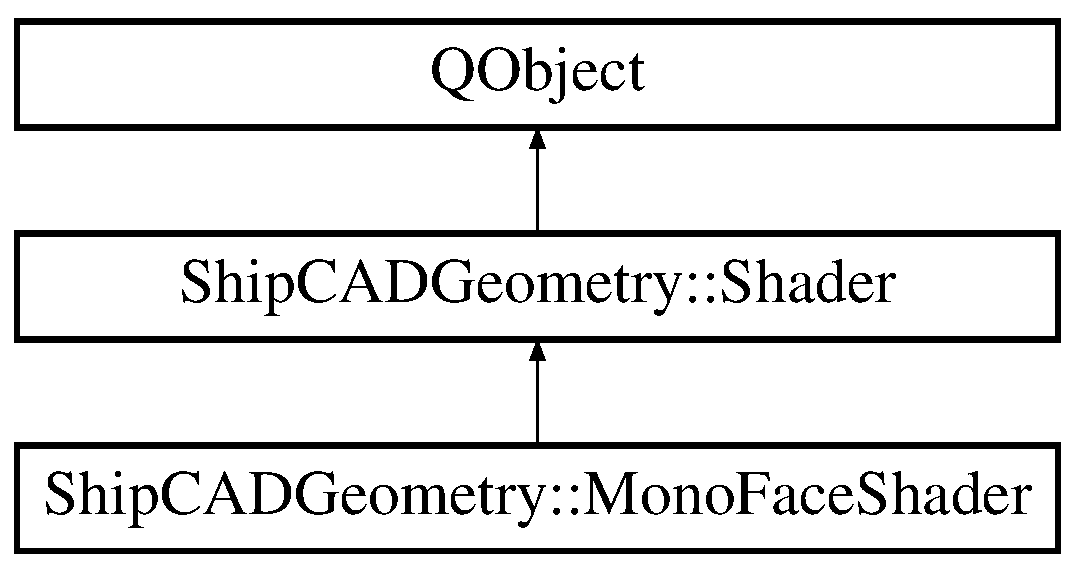
\includegraphics[height=3.000000cm]{classShipCADGeometry_1_1MonoFaceShader}
\end{center}
\end{figure}
\subsection*{Public Member Functions}
\begin{DoxyCompactItemize}
\item 
\hyperlink{classShipCADGeometry_1_1MonoFaceShader_a963aa389c930d6482a58f49b2ccb4473}{Mono\-Face\-Shader} (\hyperlink{classShipCADGeometry_1_1Viewport}{Viewport} $\ast$vp)
\item 
virtual \hyperlink{classShipCADGeometry_1_1MonoFaceShader_a3779b65915f5a7f8d60a7a78a9a6da56}{$\sim$\-Mono\-Face\-Shader} ()
\item 
virtual void \hyperlink{classShipCADGeometry_1_1MonoFaceShader_a9a358ec63af4b067449e772cbc735d5a}{render\-Mesh} (Q\-Color mesh\-Color, Q\-Vector$<$ Q\-Vector3\-D $>$ \&vertices, Q\-Vector$<$ Q\-Vector3\-D $>$ \&normals)
\end{DoxyCompactItemize}
\subsection*{Additional Inherited Members}


\subsection{Detailed Description}


Definition at line 92 of file shader.\-h.



\subsection{Constructor \& Destructor Documentation}
\hypertarget{classShipCADGeometry_1_1MonoFaceShader_a963aa389c930d6482a58f49b2ccb4473}{\index{Ship\-C\-A\-D\-Geometry\-::\-Mono\-Face\-Shader@{Ship\-C\-A\-D\-Geometry\-::\-Mono\-Face\-Shader}!Mono\-Face\-Shader@{Mono\-Face\-Shader}}
\index{Mono\-Face\-Shader@{Mono\-Face\-Shader}!ShipCADGeometry::MonoFaceShader@{Ship\-C\-A\-D\-Geometry\-::\-Mono\-Face\-Shader}}
\subsubsection[{Mono\-Face\-Shader}]{\setlength{\rightskip}{0pt plus 5cm}Mono\-Face\-Shader\-::\-Mono\-Face\-Shader (
\begin{DoxyParamCaption}
\item[{{\bf Viewport} $\ast$}]{vp}
\end{DoxyParamCaption}
)\hspace{0.3cm}{\ttfamily [explicit]}}}\label{classShipCADGeometry_1_1MonoFaceShader_a963aa389c930d6482a58f49b2ccb4473}


Definition at line 177 of file shader.\-cpp.

\hypertarget{classShipCADGeometry_1_1MonoFaceShader_a3779b65915f5a7f8d60a7a78a9a6da56}{\index{Ship\-C\-A\-D\-Geometry\-::\-Mono\-Face\-Shader@{Ship\-C\-A\-D\-Geometry\-::\-Mono\-Face\-Shader}!$\sim$\-Mono\-Face\-Shader@{$\sim$\-Mono\-Face\-Shader}}
\index{$\sim$\-Mono\-Face\-Shader@{$\sim$\-Mono\-Face\-Shader}!ShipCADGeometry::MonoFaceShader@{Ship\-C\-A\-D\-Geometry\-::\-Mono\-Face\-Shader}}
\subsubsection[{$\sim$\-Mono\-Face\-Shader}]{\setlength{\rightskip}{0pt plus 5cm}virtual Ship\-C\-A\-D\-Geometry\-::\-Mono\-Face\-Shader\-::$\sim$\-Mono\-Face\-Shader (
\begin{DoxyParamCaption}
{}
\end{DoxyParamCaption}
)\hspace{0.3cm}{\ttfamily [inline]}, {\ttfamily [virtual]}}}\label{classShipCADGeometry_1_1MonoFaceShader_a3779b65915f5a7f8d60a7a78a9a6da56}


Definition at line 99 of file shader.\-h.



\subsection{Member Function Documentation}
\hypertarget{classShipCADGeometry_1_1MonoFaceShader_a9a358ec63af4b067449e772cbc735d5a}{\index{Ship\-C\-A\-D\-Geometry\-::\-Mono\-Face\-Shader@{Ship\-C\-A\-D\-Geometry\-::\-Mono\-Face\-Shader}!render\-Mesh@{render\-Mesh}}
\index{render\-Mesh@{render\-Mesh}!ShipCADGeometry::MonoFaceShader@{Ship\-C\-A\-D\-Geometry\-::\-Mono\-Face\-Shader}}
\subsubsection[{render\-Mesh}]{\setlength{\rightskip}{0pt plus 5cm}void Mono\-Face\-Shader\-::render\-Mesh (
\begin{DoxyParamCaption}
\item[{Q\-Color}]{mesh\-Color, }
\item[{Q\-Vector$<$ Q\-Vector3\-D $>$ \&}]{vertices, }
\item[{Q\-Vector$<$ Q\-Vector3\-D $>$ \&}]{normals}
\end{DoxyParamCaption}
)\hspace{0.3cm}{\ttfamily [virtual]}}}\label{classShipCADGeometry_1_1MonoFaceShader_a9a358ec63af4b067449e772cbc735d5a}


Definition at line 188 of file shader.\-cpp.



The documentation for this class was generated from the following files\-:\begin{DoxyCompactItemize}
\item 
Ship\-C\-A\-Dlib/\hyperlink{shader_8h}{shader.\-h}\item 
Ship\-C\-A\-Dlib/\hyperlink{shader_8cpp}{shader.\-cpp}\end{DoxyCompactItemize}

\hypertarget{classShipCADGeometry_1_1NURBSurface}{\section{Ship\-C\-A\-D\-Geometry\-:\-:N\-U\-R\-B\-Surface Class Reference}
\label{classShipCADGeometry_1_1NURBSurface}\index{Ship\-C\-A\-D\-Geometry\-::\-N\-U\-R\-B\-Surface@{Ship\-C\-A\-D\-Geometry\-::\-N\-U\-R\-B\-Surface}}
}


{\ttfamily \#include $<$nurbsurface.\-h$>$}

Inheritance diagram for Ship\-C\-A\-D\-Geometry\-:\-:N\-U\-R\-B\-Surface\-:\begin{figure}[H]
\begin{center}
\leavevmode
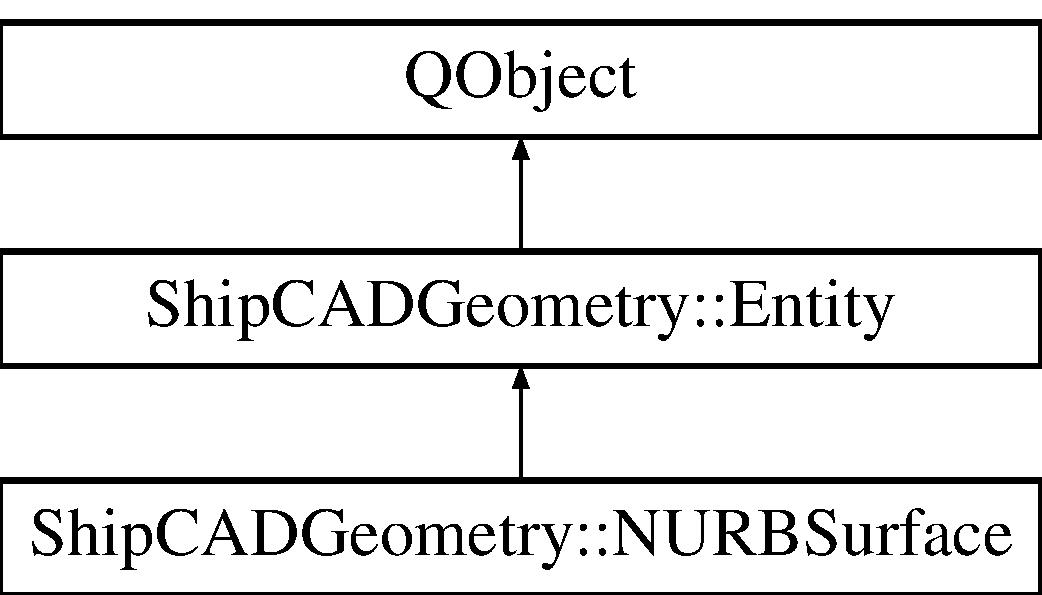
\includegraphics[height=3.000000cm]{classShipCADGeometry_1_1NURBSurface}
\end{center}
\end{figure}
\subsection*{Public Member Functions}
\begin{DoxyCompactItemize}
\item 
\hyperlink{classShipCADGeometry_1_1NURBSurface_ac01a08234a1d2a5e44d68a7393ef131c}{N\-U\-R\-B\-Surface} ()
\item 
virtual \hyperlink{classShipCADGeometry_1_1NURBSurface_ac15393324ac350b5fd544789f4e55ad0}{$\sim$\-N\-U\-R\-B\-Surface} ()
\item 
virtual void \hyperlink{classShipCADGeometry_1_1NURBSurface_a5013b0c1e511ea68909eef5d0473d032}{clear} ()
\item 
virtual void \hyperlink{classShipCADGeometry_1_1NURBSurface_a643231ea9a8f26e528a1d9a0dccf4070}{rebuild} ()
\item 
virtual void \hyperlink{classShipCADGeometry_1_1NURBSurface_a9ee8f8aea431fe9f465080ec9f5624f9}{draw} (\hyperlink{classShipCADGeometry_1_1Viewport}{Viewport} \&vp)
\item 
Q\-Vector3\-D \hyperlink{classShipCADGeometry_1_1NURBSurface_a30435ae8689f09400b7754e4d7b3242a}{get\-Point} (size\-\_\-t row, size\-\_\-t col)
\item 
void \hyperlink{classShipCADGeometry_1_1NURBSurface_a598d027e87730f815c561ae6e08f0bbe}{set\-Col\-Degree} (size\-\_\-t val)
\item 
void \hyperlink{classShipCADGeometry_1_1NURBSurface_a5b587aac512a3b6ce32bbf897256ce6f}{set\-Row\-Degree} (size\-\_\-t val)
\item 
void \hyperlink{classShipCADGeometry_1_1NURBSurface_aca43db0a1f829e101c4df124a4490031}{set\-Point} (size\-\_\-t row, size\-\_\-t col, const Q\-Vector3\-D \&val)
\item 
virtual void \hyperlink{classShipCADGeometry_1_1NURBSurface_aa6fc3d060087593349ce1b5119419433}{set\-Build} (bool val)
\item 
void \hyperlink{classShipCADGeometry_1_1NURBSurface_ad94a4350cda13ed3971ccf7bedaa1f10}{dump} (std\-::ostream \&os) const 
\end{DoxyCompactItemize}
\subsection*{Protected Attributes}
\begin{DoxyCompactItemize}
\item 
int \hyperlink{classShipCADGeometry_1_1NURBSurface_a31e27f8c4fcc7e0073fdc6d117cb3cb1}{\-\_\-col\-\_\-count}
\item 
int \hyperlink{classShipCADGeometry_1_1NURBSurface_a88c1ca0b8176d2c0a758afa936d8eaba}{\-\_\-row\-\_\-count}
\item 
int \hyperlink{classShipCADGeometry_1_1NURBSurface_a24f91b5212f2705c28bda35282ec5cb9}{\-\_\-col\-\_\-degree}
\item 
int \hyperlink{classShipCADGeometry_1_1NURBSurface_a8de52ae5ee0129c669721597b0e98adf}{\-\_\-row\-\_\-degree}
\item 
int \hyperlink{classShipCADGeometry_1_1NURBSurface_a9364be529dc16146063112608dfdd3a4}{\-\_\-col\-\_\-knots}
\item 
int \hyperlink{classShipCADGeometry_1_1NURBSurface_a79ed680d5cafd6d893e099e9e93bead2}{\-\_\-row\-\_\-knots}
\item 
std\-::vector$<$ Q\-Vector3\-D $>$ \hyperlink{classShipCADGeometry_1_1NURBSurface_ae040c228e863bedf30c7e70a94a87c27}{\-\_\-points}
\item 
std\-::vector$<$ bool $>$ \hyperlink{classShipCADGeometry_1_1NURBSurface_a9d6d1bc4ffd84dcab014313963705389}{\-\_\-knuckles}
\item 
std\-::vector$<$ float $>$ \hyperlink{classShipCADGeometry_1_1NURBSurface_a61d19bf03c2aef8db727a199308da45a}{\-\_\-parameters}
\item 
std\-::vector$<$ Q\-Vector3\-D $>$ \hyperlink{classShipCADGeometry_1_1NURBSurface_afcc62885b941c474e1217d1b9a8143b1}{\-\_\-derivatives}
\end{DoxyCompactItemize}
\subsection*{Additional Inherited Members}


\subsection{Detailed Description}


Definition at line 43 of file nurbsurface.\-h.



\subsection{Constructor \& Destructor Documentation}
\hypertarget{classShipCADGeometry_1_1NURBSurface_ac01a08234a1d2a5e44d68a7393ef131c}{\index{Ship\-C\-A\-D\-Geometry\-::\-N\-U\-R\-B\-Surface@{Ship\-C\-A\-D\-Geometry\-::\-N\-U\-R\-B\-Surface}!N\-U\-R\-B\-Surface@{N\-U\-R\-B\-Surface}}
\index{N\-U\-R\-B\-Surface@{N\-U\-R\-B\-Surface}!ShipCADGeometry::NURBSurface@{Ship\-C\-A\-D\-Geometry\-::\-N\-U\-R\-B\-Surface}}
\subsubsection[{N\-U\-R\-B\-Surface}]{\setlength{\rightskip}{0pt plus 5cm}N\-U\-R\-B\-Surface\-::\-N\-U\-R\-B\-Surface (
\begin{DoxyParamCaption}
{}
\end{DoxyParamCaption}
)\hspace{0.3cm}{\ttfamily [explicit]}}}\label{classShipCADGeometry_1_1NURBSurface_ac01a08234a1d2a5e44d68a7393ef131c}


Definition at line 40 of file nurbsurface.\-cpp.

\hypertarget{classShipCADGeometry_1_1NURBSurface_ac15393324ac350b5fd544789f4e55ad0}{\index{Ship\-C\-A\-D\-Geometry\-::\-N\-U\-R\-B\-Surface@{Ship\-C\-A\-D\-Geometry\-::\-N\-U\-R\-B\-Surface}!$\sim$\-N\-U\-R\-B\-Surface@{$\sim$\-N\-U\-R\-B\-Surface}}
\index{$\sim$\-N\-U\-R\-B\-Surface@{$\sim$\-N\-U\-R\-B\-Surface}!ShipCADGeometry::NURBSurface@{Ship\-C\-A\-D\-Geometry\-::\-N\-U\-R\-B\-Surface}}
\subsubsection[{$\sim$\-N\-U\-R\-B\-Surface}]{\setlength{\rightskip}{0pt plus 5cm}N\-U\-R\-B\-Surface\-::$\sim$\-N\-U\-R\-B\-Surface (
\begin{DoxyParamCaption}
{}
\end{DoxyParamCaption}
)\hspace{0.3cm}{\ttfamily [virtual]}}}\label{classShipCADGeometry_1_1NURBSurface_ac15393324ac350b5fd544789f4e55ad0}


Definition at line 46 of file nurbsurface.\-cpp.



\subsection{Member Function Documentation}
\hypertarget{classShipCADGeometry_1_1NURBSurface_a5013b0c1e511ea68909eef5d0473d032}{\index{Ship\-C\-A\-D\-Geometry\-::\-N\-U\-R\-B\-Surface@{Ship\-C\-A\-D\-Geometry\-::\-N\-U\-R\-B\-Surface}!clear@{clear}}
\index{clear@{clear}!ShipCADGeometry::NURBSurface@{Ship\-C\-A\-D\-Geometry\-::\-N\-U\-R\-B\-Surface}}
\subsubsection[{clear}]{\setlength{\rightskip}{0pt plus 5cm}void N\-U\-R\-B\-Surface\-::clear (
\begin{DoxyParamCaption}
{}
\end{DoxyParamCaption}
)\hspace{0.3cm}{\ttfamily [virtual]}}}\label{classShipCADGeometry_1_1NURBSurface_a5013b0c1e511ea68909eef5d0473d032}


Reimplemented from \hyperlink{classShipCADGeometry_1_1Entity_a998d0e5d360371046fd5835ba1e0877a}{Ship\-C\-A\-D\-Geometry\-::\-Entity}.



Definition at line 77 of file nurbsurface.\-cpp.

\hypertarget{classShipCADGeometry_1_1NURBSurface_a9ee8f8aea431fe9f465080ec9f5624f9}{\index{Ship\-C\-A\-D\-Geometry\-::\-N\-U\-R\-B\-Surface@{Ship\-C\-A\-D\-Geometry\-::\-N\-U\-R\-B\-Surface}!draw@{draw}}
\index{draw@{draw}!ShipCADGeometry::NURBSurface@{Ship\-C\-A\-D\-Geometry\-::\-N\-U\-R\-B\-Surface}}
\subsubsection[{draw}]{\setlength{\rightskip}{0pt plus 5cm}void N\-U\-R\-B\-Surface\-::draw (
\begin{DoxyParamCaption}
\item[{{\bf Viewport} \&}]{vp}
\end{DoxyParamCaption}
)\hspace{0.3cm}{\ttfamily [virtual]}}}\label{classShipCADGeometry_1_1NURBSurface_a9ee8f8aea431fe9f465080ec9f5624f9}


Definition at line 73 of file nurbsurface.\-cpp.

\hypertarget{classShipCADGeometry_1_1NURBSurface_ad94a4350cda13ed3971ccf7bedaa1f10}{\index{Ship\-C\-A\-D\-Geometry\-::\-N\-U\-R\-B\-Surface@{Ship\-C\-A\-D\-Geometry\-::\-N\-U\-R\-B\-Surface}!dump@{dump}}
\index{dump@{dump}!ShipCADGeometry::NURBSurface@{Ship\-C\-A\-D\-Geometry\-::\-N\-U\-R\-B\-Surface}}
\subsubsection[{dump}]{\setlength{\rightskip}{0pt plus 5cm}void N\-U\-R\-B\-Surface\-::dump (
\begin{DoxyParamCaption}
\item[{std\-::ostream \&}]{os}
\end{DoxyParamCaption}
) const}}\label{classShipCADGeometry_1_1NURBSurface_ad94a4350cda13ed3971ccf7bedaa1f10}


Definition at line 81 of file nurbsurface.\-cpp.

\hypertarget{classShipCADGeometry_1_1NURBSurface_a30435ae8689f09400b7754e4d7b3242a}{\index{Ship\-C\-A\-D\-Geometry\-::\-N\-U\-R\-B\-Surface@{Ship\-C\-A\-D\-Geometry\-::\-N\-U\-R\-B\-Surface}!get\-Point@{get\-Point}}
\index{get\-Point@{get\-Point}!ShipCADGeometry::NURBSurface@{Ship\-C\-A\-D\-Geometry\-::\-N\-U\-R\-B\-Surface}}
\subsubsection[{get\-Point}]{\setlength{\rightskip}{0pt plus 5cm}Q\-Vector3\-D N\-U\-R\-B\-Surface\-::get\-Point (
\begin{DoxyParamCaption}
\item[{size\-\_\-t}]{row, }
\item[{size\-\_\-t}]{col}
\end{DoxyParamCaption}
)}}\label{classShipCADGeometry_1_1NURBSurface_a30435ae8689f09400b7754e4d7b3242a}


Definition at line 62 of file nurbsurface.\-cpp.

\hypertarget{classShipCADGeometry_1_1NURBSurface_a643231ea9a8f26e528a1d9a0dccf4070}{\index{Ship\-C\-A\-D\-Geometry\-::\-N\-U\-R\-B\-Surface@{Ship\-C\-A\-D\-Geometry\-::\-N\-U\-R\-B\-Surface}!rebuild@{rebuild}}
\index{rebuild@{rebuild}!ShipCADGeometry::NURBSurface@{Ship\-C\-A\-D\-Geometry\-::\-N\-U\-R\-B\-Surface}}
\subsubsection[{rebuild}]{\setlength{\rightskip}{0pt plus 5cm}void N\-U\-R\-B\-Surface\-::rebuild (
\begin{DoxyParamCaption}
{}
\end{DoxyParamCaption}
)\hspace{0.3cm}{\ttfamily [virtual]}}}\label{classShipCADGeometry_1_1NURBSurface_a643231ea9a8f26e528a1d9a0dccf4070}


Implements \hyperlink{classShipCADGeometry_1_1Entity_ad49217d575c57a1fcc99768081b864ee}{Ship\-C\-A\-D\-Geometry\-::\-Entity}.



Definition at line 67 of file nurbsurface.\-cpp.

\hypertarget{classShipCADGeometry_1_1NURBSurface_aa6fc3d060087593349ce1b5119419433}{\index{Ship\-C\-A\-D\-Geometry\-::\-N\-U\-R\-B\-Surface@{Ship\-C\-A\-D\-Geometry\-::\-N\-U\-R\-B\-Surface}!set\-Build@{set\-Build}}
\index{set\-Build@{set\-Build}!ShipCADGeometry::NURBSurface@{Ship\-C\-A\-D\-Geometry\-::\-N\-U\-R\-B\-Surface}}
\subsubsection[{set\-Build}]{\setlength{\rightskip}{0pt plus 5cm}void N\-U\-R\-B\-Surface\-::set\-Build (
\begin{DoxyParamCaption}
\item[{bool}]{val}
\end{DoxyParamCaption}
)\hspace{0.3cm}{\ttfamily [virtual]}}}\label{classShipCADGeometry_1_1NURBSurface_aa6fc3d060087593349ce1b5119419433}


Reimplemented from \hyperlink{classShipCADGeometry_1_1Entity_a1889198398f42bb7f77a2334031c3f33}{Ship\-C\-A\-D\-Geometry\-::\-Entity}.



Definition at line 51 of file nurbsurface.\-cpp.

\hypertarget{classShipCADGeometry_1_1NURBSurface_a598d027e87730f815c561ae6e08f0bbe}{\index{Ship\-C\-A\-D\-Geometry\-::\-N\-U\-R\-B\-Surface@{Ship\-C\-A\-D\-Geometry\-::\-N\-U\-R\-B\-Surface}!set\-Col\-Degree@{set\-Col\-Degree}}
\index{set\-Col\-Degree@{set\-Col\-Degree}!ShipCADGeometry::NURBSurface@{Ship\-C\-A\-D\-Geometry\-::\-N\-U\-R\-B\-Surface}}
\subsubsection[{set\-Col\-Degree}]{\setlength{\rightskip}{0pt plus 5cm}void Ship\-C\-A\-D\-Geometry\-::\-N\-U\-R\-B\-Surface\-::set\-Col\-Degree (
\begin{DoxyParamCaption}
\item[{size\-\_\-t}]{val}
\end{DoxyParamCaption}
)}}\label{classShipCADGeometry_1_1NURBSurface_a598d027e87730f815c561ae6e08f0bbe}
\hypertarget{classShipCADGeometry_1_1NURBSurface_aca43db0a1f829e101c4df124a4490031}{\index{Ship\-C\-A\-D\-Geometry\-::\-N\-U\-R\-B\-Surface@{Ship\-C\-A\-D\-Geometry\-::\-N\-U\-R\-B\-Surface}!set\-Point@{set\-Point}}
\index{set\-Point@{set\-Point}!ShipCADGeometry::NURBSurface@{Ship\-C\-A\-D\-Geometry\-::\-N\-U\-R\-B\-Surface}}
\subsubsection[{set\-Point}]{\setlength{\rightskip}{0pt plus 5cm}void N\-U\-R\-B\-Surface\-::set\-Point (
\begin{DoxyParamCaption}
\item[{size\-\_\-t}]{row, }
\item[{size\-\_\-t}]{col, }
\item[{const Q\-Vector3\-D \&}]{val}
\end{DoxyParamCaption}
)}}\label{classShipCADGeometry_1_1NURBSurface_aca43db0a1f829e101c4df124a4490031}


Definition at line 58 of file nurbsurface.\-cpp.

\hypertarget{classShipCADGeometry_1_1NURBSurface_a5b587aac512a3b6ce32bbf897256ce6f}{\index{Ship\-C\-A\-D\-Geometry\-::\-N\-U\-R\-B\-Surface@{Ship\-C\-A\-D\-Geometry\-::\-N\-U\-R\-B\-Surface}!set\-Row\-Degree@{set\-Row\-Degree}}
\index{set\-Row\-Degree@{set\-Row\-Degree}!ShipCADGeometry::NURBSurface@{Ship\-C\-A\-D\-Geometry\-::\-N\-U\-R\-B\-Surface}}
\subsubsection[{set\-Row\-Degree}]{\setlength{\rightskip}{0pt plus 5cm}void Ship\-C\-A\-D\-Geometry\-::\-N\-U\-R\-B\-Surface\-::set\-Row\-Degree (
\begin{DoxyParamCaption}
\item[{size\-\_\-t}]{val}
\end{DoxyParamCaption}
)}}\label{classShipCADGeometry_1_1NURBSurface_a5b587aac512a3b6ce32bbf897256ce6f}


\subsection{Member Data Documentation}
\hypertarget{classShipCADGeometry_1_1NURBSurface_a31e27f8c4fcc7e0073fdc6d117cb3cb1}{\index{Ship\-C\-A\-D\-Geometry\-::\-N\-U\-R\-B\-Surface@{Ship\-C\-A\-D\-Geometry\-::\-N\-U\-R\-B\-Surface}!\-\_\-col\-\_\-count@{\-\_\-col\-\_\-count}}
\index{\-\_\-col\-\_\-count@{\-\_\-col\-\_\-count}!ShipCADGeometry::NURBSurface@{Ship\-C\-A\-D\-Geometry\-::\-N\-U\-R\-B\-Surface}}
\subsubsection[{\-\_\-col\-\_\-count}]{\setlength{\rightskip}{0pt plus 5cm}int Ship\-C\-A\-D\-Geometry\-::\-N\-U\-R\-B\-Surface\-::\-\_\-col\-\_\-count\hspace{0.3cm}{\ttfamily [protected]}}}\label{classShipCADGeometry_1_1NURBSurface_a31e27f8c4fcc7e0073fdc6d117cb3cb1}


Definition at line 78 of file nurbsurface.\-h.

\hypertarget{classShipCADGeometry_1_1NURBSurface_a24f91b5212f2705c28bda35282ec5cb9}{\index{Ship\-C\-A\-D\-Geometry\-::\-N\-U\-R\-B\-Surface@{Ship\-C\-A\-D\-Geometry\-::\-N\-U\-R\-B\-Surface}!\-\_\-col\-\_\-degree@{\-\_\-col\-\_\-degree}}
\index{\-\_\-col\-\_\-degree@{\-\_\-col\-\_\-degree}!ShipCADGeometry::NURBSurface@{Ship\-C\-A\-D\-Geometry\-::\-N\-U\-R\-B\-Surface}}
\subsubsection[{\-\_\-col\-\_\-degree}]{\setlength{\rightskip}{0pt plus 5cm}int Ship\-C\-A\-D\-Geometry\-::\-N\-U\-R\-B\-Surface\-::\-\_\-col\-\_\-degree\hspace{0.3cm}{\ttfamily [protected]}}}\label{classShipCADGeometry_1_1NURBSurface_a24f91b5212f2705c28bda35282ec5cb9}


Definition at line 80 of file nurbsurface.\-h.

\hypertarget{classShipCADGeometry_1_1NURBSurface_a9364be529dc16146063112608dfdd3a4}{\index{Ship\-C\-A\-D\-Geometry\-::\-N\-U\-R\-B\-Surface@{Ship\-C\-A\-D\-Geometry\-::\-N\-U\-R\-B\-Surface}!\-\_\-col\-\_\-knots@{\-\_\-col\-\_\-knots}}
\index{\-\_\-col\-\_\-knots@{\-\_\-col\-\_\-knots}!ShipCADGeometry::NURBSurface@{Ship\-C\-A\-D\-Geometry\-::\-N\-U\-R\-B\-Surface}}
\subsubsection[{\-\_\-col\-\_\-knots}]{\setlength{\rightskip}{0pt plus 5cm}int Ship\-C\-A\-D\-Geometry\-::\-N\-U\-R\-B\-Surface\-::\-\_\-col\-\_\-knots\hspace{0.3cm}{\ttfamily [protected]}}}\label{classShipCADGeometry_1_1NURBSurface_a9364be529dc16146063112608dfdd3a4}


Definition at line 82 of file nurbsurface.\-h.

\hypertarget{classShipCADGeometry_1_1NURBSurface_afcc62885b941c474e1217d1b9a8143b1}{\index{Ship\-C\-A\-D\-Geometry\-::\-N\-U\-R\-B\-Surface@{Ship\-C\-A\-D\-Geometry\-::\-N\-U\-R\-B\-Surface}!\-\_\-derivatives@{\-\_\-derivatives}}
\index{\-\_\-derivatives@{\-\_\-derivatives}!ShipCADGeometry::NURBSurface@{Ship\-C\-A\-D\-Geometry\-::\-N\-U\-R\-B\-Surface}}
\subsubsection[{\-\_\-derivatives}]{\setlength{\rightskip}{0pt plus 5cm}std\-::vector$<$Q\-Vector3\-D$>$ Ship\-C\-A\-D\-Geometry\-::\-N\-U\-R\-B\-Surface\-::\-\_\-derivatives\hspace{0.3cm}{\ttfamily [protected]}}}\label{classShipCADGeometry_1_1NURBSurface_afcc62885b941c474e1217d1b9a8143b1}


Definition at line 88 of file nurbsurface.\-h.

\hypertarget{classShipCADGeometry_1_1NURBSurface_a9d6d1bc4ffd84dcab014313963705389}{\index{Ship\-C\-A\-D\-Geometry\-::\-N\-U\-R\-B\-Surface@{Ship\-C\-A\-D\-Geometry\-::\-N\-U\-R\-B\-Surface}!\-\_\-knuckles@{\-\_\-knuckles}}
\index{\-\_\-knuckles@{\-\_\-knuckles}!ShipCADGeometry::NURBSurface@{Ship\-C\-A\-D\-Geometry\-::\-N\-U\-R\-B\-Surface}}
\subsubsection[{\-\_\-knuckles}]{\setlength{\rightskip}{0pt plus 5cm}std\-::vector$<$bool$>$ Ship\-C\-A\-D\-Geometry\-::\-N\-U\-R\-B\-Surface\-::\-\_\-knuckles\hspace{0.3cm}{\ttfamily [protected]}}}\label{classShipCADGeometry_1_1NURBSurface_a9d6d1bc4ffd84dcab014313963705389}


Definition at line 86 of file nurbsurface.\-h.

\hypertarget{classShipCADGeometry_1_1NURBSurface_a61d19bf03c2aef8db727a199308da45a}{\index{Ship\-C\-A\-D\-Geometry\-::\-N\-U\-R\-B\-Surface@{Ship\-C\-A\-D\-Geometry\-::\-N\-U\-R\-B\-Surface}!\-\_\-parameters@{\-\_\-parameters}}
\index{\-\_\-parameters@{\-\_\-parameters}!ShipCADGeometry::NURBSurface@{Ship\-C\-A\-D\-Geometry\-::\-N\-U\-R\-B\-Surface}}
\subsubsection[{\-\_\-parameters}]{\setlength{\rightskip}{0pt plus 5cm}std\-::vector$<$float$>$ Ship\-C\-A\-D\-Geometry\-::\-N\-U\-R\-B\-Surface\-::\-\_\-parameters\hspace{0.3cm}{\ttfamily [protected]}}}\label{classShipCADGeometry_1_1NURBSurface_a61d19bf03c2aef8db727a199308da45a}


Definition at line 87 of file nurbsurface.\-h.

\hypertarget{classShipCADGeometry_1_1NURBSurface_ae040c228e863bedf30c7e70a94a87c27}{\index{Ship\-C\-A\-D\-Geometry\-::\-N\-U\-R\-B\-Surface@{Ship\-C\-A\-D\-Geometry\-::\-N\-U\-R\-B\-Surface}!\-\_\-points@{\-\_\-points}}
\index{\-\_\-points@{\-\_\-points}!ShipCADGeometry::NURBSurface@{Ship\-C\-A\-D\-Geometry\-::\-N\-U\-R\-B\-Surface}}
\subsubsection[{\-\_\-points}]{\setlength{\rightskip}{0pt plus 5cm}std\-::vector$<$Q\-Vector3\-D$>$ Ship\-C\-A\-D\-Geometry\-::\-N\-U\-R\-B\-Surface\-::\-\_\-points\hspace{0.3cm}{\ttfamily [protected]}}}\label{classShipCADGeometry_1_1NURBSurface_ae040c228e863bedf30c7e70a94a87c27}


Definition at line 85 of file nurbsurface.\-h.

\hypertarget{classShipCADGeometry_1_1NURBSurface_a88c1ca0b8176d2c0a758afa936d8eaba}{\index{Ship\-C\-A\-D\-Geometry\-::\-N\-U\-R\-B\-Surface@{Ship\-C\-A\-D\-Geometry\-::\-N\-U\-R\-B\-Surface}!\-\_\-row\-\_\-count@{\-\_\-row\-\_\-count}}
\index{\-\_\-row\-\_\-count@{\-\_\-row\-\_\-count}!ShipCADGeometry::NURBSurface@{Ship\-C\-A\-D\-Geometry\-::\-N\-U\-R\-B\-Surface}}
\subsubsection[{\-\_\-row\-\_\-count}]{\setlength{\rightskip}{0pt plus 5cm}int Ship\-C\-A\-D\-Geometry\-::\-N\-U\-R\-B\-Surface\-::\-\_\-row\-\_\-count\hspace{0.3cm}{\ttfamily [protected]}}}\label{classShipCADGeometry_1_1NURBSurface_a88c1ca0b8176d2c0a758afa936d8eaba}


Definition at line 79 of file nurbsurface.\-h.

\hypertarget{classShipCADGeometry_1_1NURBSurface_a8de52ae5ee0129c669721597b0e98adf}{\index{Ship\-C\-A\-D\-Geometry\-::\-N\-U\-R\-B\-Surface@{Ship\-C\-A\-D\-Geometry\-::\-N\-U\-R\-B\-Surface}!\-\_\-row\-\_\-degree@{\-\_\-row\-\_\-degree}}
\index{\-\_\-row\-\_\-degree@{\-\_\-row\-\_\-degree}!ShipCADGeometry::NURBSurface@{Ship\-C\-A\-D\-Geometry\-::\-N\-U\-R\-B\-Surface}}
\subsubsection[{\-\_\-row\-\_\-degree}]{\setlength{\rightskip}{0pt plus 5cm}int Ship\-C\-A\-D\-Geometry\-::\-N\-U\-R\-B\-Surface\-::\-\_\-row\-\_\-degree\hspace{0.3cm}{\ttfamily [protected]}}}\label{classShipCADGeometry_1_1NURBSurface_a8de52ae5ee0129c669721597b0e98adf}


Definition at line 81 of file nurbsurface.\-h.

\hypertarget{classShipCADGeometry_1_1NURBSurface_a79ed680d5cafd6d893e099e9e93bead2}{\index{Ship\-C\-A\-D\-Geometry\-::\-N\-U\-R\-B\-Surface@{Ship\-C\-A\-D\-Geometry\-::\-N\-U\-R\-B\-Surface}!\-\_\-row\-\_\-knots@{\-\_\-row\-\_\-knots}}
\index{\-\_\-row\-\_\-knots@{\-\_\-row\-\_\-knots}!ShipCADGeometry::NURBSurface@{Ship\-C\-A\-D\-Geometry\-::\-N\-U\-R\-B\-Surface}}
\subsubsection[{\-\_\-row\-\_\-knots}]{\setlength{\rightskip}{0pt plus 5cm}int Ship\-C\-A\-D\-Geometry\-::\-N\-U\-R\-B\-Surface\-::\-\_\-row\-\_\-knots\hspace{0.3cm}{\ttfamily [protected]}}}\label{classShipCADGeometry_1_1NURBSurface_a79ed680d5cafd6d893e099e9e93bead2}


Definition at line 83 of file nurbsurface.\-h.



The documentation for this class was generated from the following files\-:\begin{DoxyCompactItemize}
\item 
Ship\-C\-A\-Dlib/\hyperlink{nurbsurface_8h}{nurbsurface.\-h}\item 
Ship\-C\-A\-Dlib/\hyperlink{nurbsurface_8cpp}{nurbsurface.\-cpp}\end{DoxyCompactItemize}

\hypertarget{classOpenGLWindow}{\section{Open\-G\-L\-Window Class Reference}
\label{classOpenGLWindow}\index{Open\-G\-L\-Window@{Open\-G\-L\-Window}}
}


{\ttfamily \#include $<$openglwindow.\-h$>$}

Inheritance diagram for Open\-G\-L\-Window\-:\begin{figure}[H]
\begin{center}
\leavevmode
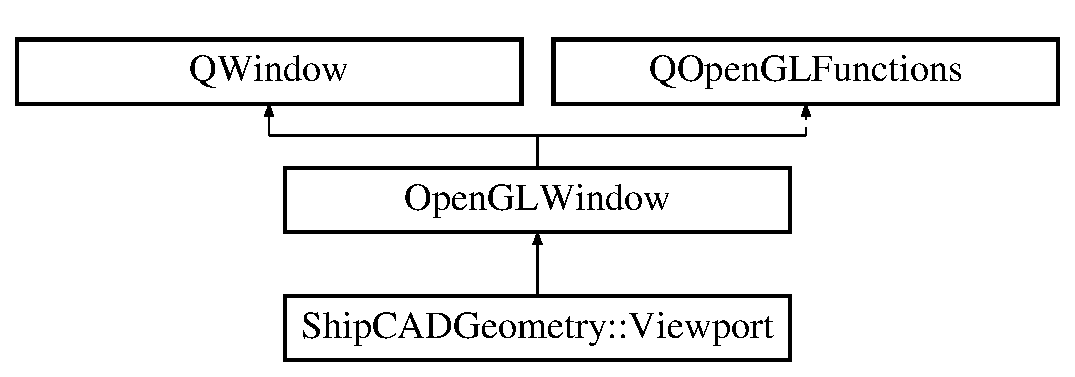
\includegraphics[height=3.000000cm]{classOpenGLWindow}
\end{center}
\end{figure}
\subsection*{Public Slots}
\begin{DoxyCompactItemize}
\item 
void \hyperlink{classOpenGLWindow_abea9e50147496e5110b86f03122fbece}{render\-Later} ()
\item 
void \hyperlink{classOpenGLWindow_a8398ed62d646739fe54fae94c477ad1d}{render\-Now} ()
\end{DoxyCompactItemize}
\subsection*{Public Member Functions}
\begin{DoxyCompactItemize}
\item 
\hyperlink{classOpenGLWindow_a90bb7dbb2dcb27b1fdc56ef4ef3f25fc}{Open\-G\-L\-Window} (Q\-Window $\ast$parent=0)
\item 
\hyperlink{classOpenGLWindow_aa220b192c71871aab9100f4058a8d62d}{$\sim$\-Open\-G\-L\-Window} ()
\item 
virtual void \hyperlink{classOpenGLWindow_a186cffcb57053e4eda4875b1ab9aac92}{render} (Q\-Painter $\ast$painter)
\item 
virtual void \hyperlink{classOpenGLWindow_ac9e094864803a0b29364f42c2a47fa8c}{render} ()
\item 
virtual void \hyperlink{classOpenGLWindow_aed4e2ee22e113b2f7e7d1eba4ef1b965}{initialize} ()
\item 
void \hyperlink{classOpenGLWindow_a68317e3284d7b0ffba262eac059b6b9e}{set\-Animating} (bool animating)
\end{DoxyCompactItemize}
\subsection*{Protected Member Functions}
\begin{DoxyCompactItemize}
\item 
bool \hyperlink{classOpenGLWindow_a1e3045cffb900de55b7384f5091c9d94}{event} (Q\-Event $\ast$event)
\item 
void \hyperlink{classOpenGLWindow_a991121ba7a4bbfa208fa74e5c86004c3}{expose\-Event} (Q\-Expose\-Event $\ast$\hyperlink{classOpenGLWindow_a1e3045cffb900de55b7384f5091c9d94}{event})
\item 
void \hyperlink{classOpenGLWindow_ae0e1d4dc039ce114ac615ce1dee38e51}{resize\-Event} (Q\-Resize\-Event $\ast$\hyperlink{classOpenGLWindow_a1e3045cffb900de55b7384f5091c9d94}{event})
\end{DoxyCompactItemize}


\subsection{Detailed Description}


Definition at line 75 of file openglwindow.\-h.



\subsection{Constructor \& Destructor Documentation}
\hypertarget{classOpenGLWindow_a90bb7dbb2dcb27b1fdc56ef4ef3f25fc}{\index{Open\-G\-L\-Window@{Open\-G\-L\-Window}!Open\-G\-L\-Window@{Open\-G\-L\-Window}}
\index{Open\-G\-L\-Window@{Open\-G\-L\-Window}!OpenGLWindow@{Open\-G\-L\-Window}}
\subsubsection[{Open\-G\-L\-Window}]{\setlength{\rightskip}{0pt plus 5cm}Open\-G\-L\-Window\-::\-Open\-G\-L\-Window (
\begin{DoxyParamCaption}
\item[{Q\-Window $\ast$}]{parent = {\ttfamily 0}}
\end{DoxyParamCaption}
)\hspace{0.3cm}{\ttfamily [explicit]}}}\label{classOpenGLWindow_a90bb7dbb2dcb27b1fdc56ef4ef3f25fc}


Definition at line 76 of file openglwindow.\-cpp.

\hypertarget{classOpenGLWindow_aa220b192c71871aab9100f4058a8d62d}{\index{Open\-G\-L\-Window@{Open\-G\-L\-Window}!$\sim$\-Open\-G\-L\-Window@{$\sim$\-Open\-G\-L\-Window}}
\index{$\sim$\-Open\-G\-L\-Window@{$\sim$\-Open\-G\-L\-Window}!OpenGLWindow@{Open\-G\-L\-Window}}
\subsubsection[{$\sim$\-Open\-G\-L\-Window}]{\setlength{\rightskip}{0pt plus 5cm}Open\-G\-L\-Window\-::$\sim$\-Open\-G\-L\-Window (
\begin{DoxyParamCaption}
{}
\end{DoxyParamCaption}
)}}\label{classOpenGLWindow_aa220b192c71871aab9100f4058a8d62d}


Definition at line 86 of file openglwindow.\-cpp.



\subsection{Member Function Documentation}
\hypertarget{classOpenGLWindow_a1e3045cffb900de55b7384f5091c9d94}{\index{Open\-G\-L\-Window@{Open\-G\-L\-Window}!event@{event}}
\index{event@{event}!OpenGLWindow@{Open\-G\-L\-Window}}
\subsubsection[{event}]{\setlength{\rightskip}{0pt plus 5cm}bool Open\-G\-L\-Window\-::event (
\begin{DoxyParamCaption}
\item[{Q\-Event $\ast$}]{event}
\end{DoxyParamCaption}
)\hspace{0.3cm}{\ttfamily [protected]}}}\label{classOpenGLWindow_a1e3045cffb900de55b7384f5091c9d94}


Definition at line 120 of file openglwindow.\-cpp.

\hypertarget{classOpenGLWindow_a991121ba7a4bbfa208fa74e5c86004c3}{\index{Open\-G\-L\-Window@{Open\-G\-L\-Window}!expose\-Event@{expose\-Event}}
\index{expose\-Event@{expose\-Event}!OpenGLWindow@{Open\-G\-L\-Window}}
\subsubsection[{expose\-Event}]{\setlength{\rightskip}{0pt plus 5cm}void Open\-G\-L\-Window\-::expose\-Event (
\begin{DoxyParamCaption}
\item[{Q\-Expose\-Event $\ast$}]{event}
\end{DoxyParamCaption}
)\hspace{0.3cm}{\ttfamily [protected]}}}\label{classOpenGLWindow_a991121ba7a4bbfa208fa74e5c86004c3}


Definition at line 131 of file openglwindow.\-cpp.

\hypertarget{classOpenGLWindow_aed4e2ee22e113b2f7e7d1eba4ef1b965}{\index{Open\-G\-L\-Window@{Open\-G\-L\-Window}!initialize@{initialize}}
\index{initialize@{initialize}!OpenGLWindow@{Open\-G\-L\-Window}}
\subsubsection[{initialize}]{\setlength{\rightskip}{0pt plus 5cm}void Open\-G\-L\-Window\-::initialize (
\begin{DoxyParamCaption}
{}
\end{DoxyParamCaption}
)\hspace{0.3cm}{\ttfamily [virtual]}}}\label{classOpenGLWindow_aed4e2ee22e113b2f7e7d1eba4ef1b965}


Reimplemented in \hyperlink{classShipCAD_1_1Viewport_a9c35de3f7c9d7c860c494081b48309b3}{Ship\-C\-A\-D\-::\-Viewport}.



Definition at line 95 of file openglwindow.\-cpp.

\hypertarget{classOpenGLWindow_a186cffcb57053e4eda4875b1ab9aac92}{\index{Open\-G\-L\-Window@{Open\-G\-L\-Window}!render@{render}}
\index{render@{render}!OpenGLWindow@{Open\-G\-L\-Window}}
\subsubsection[{render}]{\setlength{\rightskip}{0pt plus 5cm}void Open\-G\-L\-Window\-::render (
\begin{DoxyParamCaption}
\item[{Q\-Painter $\ast$}]{painter}
\end{DoxyParamCaption}
)\hspace{0.3cm}{\ttfamily [virtual]}}}\label{classOpenGLWindow_a186cffcb57053e4eda4875b1ab9aac92}


Definition at line 90 of file openglwindow.\-cpp.

\hypertarget{classOpenGLWindow_ac9e094864803a0b29364f42c2a47fa8c}{\index{Open\-G\-L\-Window@{Open\-G\-L\-Window}!render@{render}}
\index{render@{render}!OpenGLWindow@{Open\-G\-L\-Window}}
\subsubsection[{render}]{\setlength{\rightskip}{0pt plus 5cm}void Open\-G\-L\-Window\-::render (
\begin{DoxyParamCaption}
{}
\end{DoxyParamCaption}
)\hspace{0.3cm}{\ttfamily [virtual]}}}\label{classOpenGLWindow_ac9e094864803a0b29364f42c2a47fa8c}


Reimplemented in \hyperlink{classShipCAD_1_1Viewport_a9e81b526db3c2b508322c29b9fda5845}{Ship\-C\-A\-D\-::\-Viewport}.



Definition at line 99 of file openglwindow.\-cpp.

\hypertarget{classOpenGLWindow_abea9e50147496e5110b86f03122fbece}{\index{Open\-G\-L\-Window@{Open\-G\-L\-Window}!render\-Later@{render\-Later}}
\index{render\-Later@{render\-Later}!OpenGLWindow@{Open\-G\-L\-Window}}
\subsubsection[{render\-Later}]{\setlength{\rightskip}{0pt plus 5cm}void Open\-G\-L\-Window\-::render\-Later (
\begin{DoxyParamCaption}
{}
\end{DoxyParamCaption}
)\hspace{0.3cm}{\ttfamily [slot]}}}\label{classOpenGLWindow_abea9e50147496e5110b86f03122fbece}


Definition at line 112 of file openglwindow.\-cpp.

\hypertarget{classOpenGLWindow_a8398ed62d646739fe54fae94c477ad1d}{\index{Open\-G\-L\-Window@{Open\-G\-L\-Window}!render\-Now@{render\-Now}}
\index{render\-Now@{render\-Now}!OpenGLWindow@{Open\-G\-L\-Window}}
\subsubsection[{render\-Now}]{\setlength{\rightskip}{0pt plus 5cm}void Open\-G\-L\-Window\-::render\-Now (
\begin{DoxyParamCaption}
{}
\end{DoxyParamCaption}
)\hspace{0.3cm}{\ttfamily [slot]}}}\label{classOpenGLWindow_a8398ed62d646739fe54fae94c477ad1d}


Definition at line 147 of file openglwindow.\-cpp.

\hypertarget{classOpenGLWindow_ae0e1d4dc039ce114ac615ce1dee38e51}{\index{Open\-G\-L\-Window@{Open\-G\-L\-Window}!resize\-Event@{resize\-Event}}
\index{resize\-Event@{resize\-Event}!OpenGLWindow@{Open\-G\-L\-Window}}
\subsubsection[{resize\-Event}]{\setlength{\rightskip}{0pt plus 5cm}void Open\-G\-L\-Window\-::resize\-Event (
\begin{DoxyParamCaption}
\item[{Q\-Resize\-Event $\ast$}]{event}
\end{DoxyParamCaption}
)\hspace{0.3cm}{\ttfamily [protected]}}}\label{classOpenGLWindow_ae0e1d4dc039ce114ac615ce1dee38e51}


Definition at line 139 of file openglwindow.\-cpp.

\hypertarget{classOpenGLWindow_a68317e3284d7b0ffba262eac059b6b9e}{\index{Open\-G\-L\-Window@{Open\-G\-L\-Window}!set\-Animating@{set\-Animating}}
\index{set\-Animating@{set\-Animating}!OpenGLWindow@{Open\-G\-L\-Window}}
\subsubsection[{set\-Animating}]{\setlength{\rightskip}{0pt plus 5cm}void Open\-G\-L\-Window\-::set\-Animating (
\begin{DoxyParamCaption}
\item[{bool}]{animating}
\end{DoxyParamCaption}
)}}\label{classOpenGLWindow_a68317e3284d7b0ffba262eac059b6b9e}


Definition at line 179 of file openglwindow.\-cpp.



The documentation for this class was generated from the following files\-:\begin{DoxyCompactItemize}
\item 
Ship\-C\-A\-Dlib/\hyperlink{openglwindow_8h}{openglwindow.\-h}\item 
Ship\-C\-A\-Dlib/\hyperlink{openglwindow_8cpp}{openglwindow.\-cpp}\end{DoxyCompactItemize}

\hypertarget{classShipCADGeometry_1_1Plane}{\section{Ship\-C\-A\-D\-Geometry\-:\-:Plane Class Reference}
\label{classShipCADGeometry_1_1Plane}\index{Ship\-C\-A\-D\-Geometry\-::\-Plane@{Ship\-C\-A\-D\-Geometry\-::\-Plane}}
}


{\ttfamily \#include $<$plane.\-h$>$}

\subsection*{Public Member Functions}
\begin{DoxyCompactItemize}
\item 
\hyperlink{classShipCADGeometry_1_1Plane_acac0d9c003e0ab10d07b146c3566a0c7}{Plane} ()
\item 
\hyperlink{classShipCADGeometry_1_1Plane_a9a1420228e8baa632c7e8ba66f27772f}{Plane} (float \hyperlink{classShipCADGeometry_1_1Plane_a10415ad5e7667357729cc959e0996b30}{a}, float \hyperlink{classShipCADGeometry_1_1Plane_a5613d841f9e3c6af069f0beaf1a7c0fd}{b}, float \hyperlink{classShipCADGeometry_1_1Plane_aeedccb0995b432ba91083334d8458501}{c}, float \hyperlink{classShipCADGeometry_1_1Plane_a947034d0487902addd31d38d1556d4aa}{d})
\item 
\hyperlink{classShipCADGeometry_1_1Plane_adbaa1f5c7100e5592312359cb8eede37}{Plane} (const Q\-Vector3\-D \&p1, const Q\-Vector3\-D \&p2, const Q\-Vector3\-D \&p3)
\item 
\hyperlink{classShipCADGeometry_1_1Plane_ac89b14d37d595f51d24325a40488f927}{$\sim$\-Plane} ()
\item 
float \hyperlink{classShipCADGeometry_1_1Plane_a10415ad5e7667357729cc959e0996b30}{a} () const 
\item 
float \hyperlink{classShipCADGeometry_1_1Plane_a5613d841f9e3c6af069f0beaf1a7c0fd}{b} () const 
\item 
float \hyperlink{classShipCADGeometry_1_1Plane_aeedccb0995b432ba91083334d8458501}{c} () const 
\item 
float \hyperlink{classShipCADGeometry_1_1Plane_a947034d0487902addd31d38d1556d4aa}{d} () const 
\item 
void \hyperlink{classShipCADGeometry_1_1Plane_aa4741e4b523f68f17585580883e3b0bc}{set\-A} (float val)
\item 
void \hyperlink{classShipCADGeometry_1_1Plane_a629fb660d7053b4efa09e0eb8c21b093}{set\-B} (float val)
\item 
void \hyperlink{classShipCADGeometry_1_1Plane_a2e7b8636aa78d21630e3419933c0d0f2}{set\-C} (float val)
\item 
void \hyperlink{classShipCADGeometry_1_1Plane_a6920a08fe9e29c4fbf264f258e27ffa7}{set\-D} (float val)
\item 
float \hyperlink{classShipCADGeometry_1_1Plane_a6851b997a300848fcb37b33407165c44}{distance} (const Q\-Vector3\-D \&point) const 
\item 
bool \hyperlink{classShipCADGeometry_1_1Plane_a76d5f22d213962e8ab0880fae3e919df}{intersects\-Box} (const Q\-Vector3\-D \&p1, const Q\-Vector3\-D \&p2) const 
\end{DoxyCompactItemize}


\subsection{Detailed Description}


Definition at line 39 of file plane.\-h.



\subsection{Constructor \& Destructor Documentation}
\hypertarget{classShipCADGeometry_1_1Plane_acac0d9c003e0ab10d07b146c3566a0c7}{\index{Ship\-C\-A\-D\-Geometry\-::\-Plane@{Ship\-C\-A\-D\-Geometry\-::\-Plane}!Plane@{Plane}}
\index{Plane@{Plane}!ShipCADGeometry::Plane@{Ship\-C\-A\-D\-Geometry\-::\-Plane}}
\subsubsection[{Plane}]{\setlength{\rightskip}{0pt plus 5cm}Plane\-::\-Plane (
\begin{DoxyParamCaption}
{}
\end{DoxyParamCaption}
)\hspace{0.3cm}{\ttfamily [explicit]}}}\label{classShipCADGeometry_1_1Plane_acac0d9c003e0ab10d07b146c3566a0c7}


Definition at line 36 of file plane.\-cpp.

\hypertarget{classShipCADGeometry_1_1Plane_a9a1420228e8baa632c7e8ba66f27772f}{\index{Ship\-C\-A\-D\-Geometry\-::\-Plane@{Ship\-C\-A\-D\-Geometry\-::\-Plane}!Plane@{Plane}}
\index{Plane@{Plane}!ShipCADGeometry::Plane@{Ship\-C\-A\-D\-Geometry\-::\-Plane}}
\subsubsection[{Plane}]{\setlength{\rightskip}{0pt plus 5cm}Plane\-::\-Plane (
\begin{DoxyParamCaption}
\item[{float}]{a, }
\item[{float}]{b, }
\item[{float}]{c, }
\item[{float}]{d}
\end{DoxyParamCaption}
)\hspace{0.3cm}{\ttfamily [explicit]}}}\label{classShipCADGeometry_1_1Plane_a9a1420228e8baa632c7e8ba66f27772f}


Definition at line 41 of file plane.\-cpp.

\hypertarget{classShipCADGeometry_1_1Plane_adbaa1f5c7100e5592312359cb8eede37}{\index{Ship\-C\-A\-D\-Geometry\-::\-Plane@{Ship\-C\-A\-D\-Geometry\-::\-Plane}!Plane@{Plane}}
\index{Plane@{Plane}!ShipCADGeometry::Plane@{Ship\-C\-A\-D\-Geometry\-::\-Plane}}
\subsubsection[{Plane}]{\setlength{\rightskip}{0pt plus 5cm}Plane\-::\-Plane (
\begin{DoxyParamCaption}
\item[{const Q\-Vector3\-D \&}]{p1, }
\item[{const Q\-Vector3\-D \&}]{p2, }
\item[{const Q\-Vector3\-D \&}]{p3}
\end{DoxyParamCaption}
)\hspace{0.3cm}{\ttfamily [explicit]}}}\label{classShipCADGeometry_1_1Plane_adbaa1f5c7100e5592312359cb8eede37}


Definition at line 49 of file plane.\-cpp.

\hypertarget{classShipCADGeometry_1_1Plane_ac89b14d37d595f51d24325a40488f927}{\index{Ship\-C\-A\-D\-Geometry\-::\-Plane@{Ship\-C\-A\-D\-Geometry\-::\-Plane}!$\sim$\-Plane@{$\sim$\-Plane}}
\index{$\sim$\-Plane@{$\sim$\-Plane}!ShipCADGeometry::Plane@{Ship\-C\-A\-D\-Geometry\-::\-Plane}}
\subsubsection[{$\sim$\-Plane}]{\setlength{\rightskip}{0pt plus 5cm}Ship\-C\-A\-D\-Geometry\-::\-Plane\-::$\sim$\-Plane (
\begin{DoxyParamCaption}
{}
\end{DoxyParamCaption}
)\hspace{0.3cm}{\ttfamily [inline]}}}\label{classShipCADGeometry_1_1Plane_ac89b14d37d595f51d24325a40488f927}


Definition at line 47 of file plane.\-h.



\subsection{Member Function Documentation}
\hypertarget{classShipCADGeometry_1_1Plane_a10415ad5e7667357729cc959e0996b30}{\index{Ship\-C\-A\-D\-Geometry\-::\-Plane@{Ship\-C\-A\-D\-Geometry\-::\-Plane}!a@{a}}
\index{a@{a}!ShipCADGeometry::Plane@{Ship\-C\-A\-D\-Geometry\-::\-Plane}}
\subsubsection[{a}]{\setlength{\rightskip}{0pt plus 5cm}float Ship\-C\-A\-D\-Geometry\-::\-Plane\-::a (
\begin{DoxyParamCaption}
{}
\end{DoxyParamCaption}
) const\hspace{0.3cm}{\ttfamily [inline]}}}\label{classShipCADGeometry_1_1Plane_a10415ad5e7667357729cc959e0996b30}


Definition at line 49 of file plane.\-h.

\hypertarget{classShipCADGeometry_1_1Plane_a5613d841f9e3c6af069f0beaf1a7c0fd}{\index{Ship\-C\-A\-D\-Geometry\-::\-Plane@{Ship\-C\-A\-D\-Geometry\-::\-Plane}!b@{b}}
\index{b@{b}!ShipCADGeometry::Plane@{Ship\-C\-A\-D\-Geometry\-::\-Plane}}
\subsubsection[{b}]{\setlength{\rightskip}{0pt plus 5cm}float Ship\-C\-A\-D\-Geometry\-::\-Plane\-::b (
\begin{DoxyParamCaption}
{}
\end{DoxyParamCaption}
) const\hspace{0.3cm}{\ttfamily [inline]}}}\label{classShipCADGeometry_1_1Plane_a5613d841f9e3c6af069f0beaf1a7c0fd}


Definition at line 51 of file plane.\-h.

\hypertarget{classShipCADGeometry_1_1Plane_aeedccb0995b432ba91083334d8458501}{\index{Ship\-C\-A\-D\-Geometry\-::\-Plane@{Ship\-C\-A\-D\-Geometry\-::\-Plane}!c@{c}}
\index{c@{c}!ShipCADGeometry::Plane@{Ship\-C\-A\-D\-Geometry\-::\-Plane}}
\subsubsection[{c}]{\setlength{\rightskip}{0pt plus 5cm}float Ship\-C\-A\-D\-Geometry\-::\-Plane\-::c (
\begin{DoxyParamCaption}
{}
\end{DoxyParamCaption}
) const\hspace{0.3cm}{\ttfamily [inline]}}}\label{classShipCADGeometry_1_1Plane_aeedccb0995b432ba91083334d8458501}


Definition at line 53 of file plane.\-h.

\hypertarget{classShipCADGeometry_1_1Plane_a947034d0487902addd31d38d1556d4aa}{\index{Ship\-C\-A\-D\-Geometry\-::\-Plane@{Ship\-C\-A\-D\-Geometry\-::\-Plane}!d@{d}}
\index{d@{d}!ShipCADGeometry::Plane@{Ship\-C\-A\-D\-Geometry\-::\-Plane}}
\subsubsection[{d}]{\setlength{\rightskip}{0pt plus 5cm}float Ship\-C\-A\-D\-Geometry\-::\-Plane\-::d (
\begin{DoxyParamCaption}
{}
\end{DoxyParamCaption}
) const\hspace{0.3cm}{\ttfamily [inline]}}}\label{classShipCADGeometry_1_1Plane_a947034d0487902addd31d38d1556d4aa}


Definition at line 55 of file plane.\-h.

\hypertarget{classShipCADGeometry_1_1Plane_a6851b997a300848fcb37b33407165c44}{\index{Ship\-C\-A\-D\-Geometry\-::\-Plane@{Ship\-C\-A\-D\-Geometry\-::\-Plane}!distance@{distance}}
\index{distance@{distance}!ShipCADGeometry::Plane@{Ship\-C\-A\-D\-Geometry\-::\-Plane}}
\subsubsection[{distance}]{\setlength{\rightskip}{0pt plus 5cm}float Plane\-::distance (
\begin{DoxyParamCaption}
\item[{const Q\-Vector3\-D \&}]{point}
\end{DoxyParamCaption}
) const}}\label{classShipCADGeometry_1_1Plane_a6851b997a300848fcb37b33407165c44}


Definition at line 63 of file plane.\-cpp.

\hypertarget{classShipCADGeometry_1_1Plane_a76d5f22d213962e8ab0880fae3e919df}{\index{Ship\-C\-A\-D\-Geometry\-::\-Plane@{Ship\-C\-A\-D\-Geometry\-::\-Plane}!intersects\-Box@{intersects\-Box}}
\index{intersects\-Box@{intersects\-Box}!ShipCADGeometry::Plane@{Ship\-C\-A\-D\-Geometry\-::\-Plane}}
\subsubsection[{intersects\-Box}]{\setlength{\rightskip}{0pt plus 5cm}bool Plane\-::intersects\-Box (
\begin{DoxyParamCaption}
\item[{const Q\-Vector3\-D \&}]{p1, }
\item[{const Q\-Vector3\-D \&}]{p2}
\end{DoxyParamCaption}
) const}}\label{classShipCADGeometry_1_1Plane_a76d5f22d213962e8ab0880fae3e919df}


Definition at line 69 of file plane.\-cpp.

\hypertarget{classShipCADGeometry_1_1Plane_aa4741e4b523f68f17585580883e3b0bc}{\index{Ship\-C\-A\-D\-Geometry\-::\-Plane@{Ship\-C\-A\-D\-Geometry\-::\-Plane}!set\-A@{set\-A}}
\index{set\-A@{set\-A}!ShipCADGeometry::Plane@{Ship\-C\-A\-D\-Geometry\-::\-Plane}}
\subsubsection[{set\-A}]{\setlength{\rightskip}{0pt plus 5cm}void Ship\-C\-A\-D\-Geometry\-::\-Plane\-::set\-A (
\begin{DoxyParamCaption}
\item[{float}]{val}
\end{DoxyParamCaption}
)\hspace{0.3cm}{\ttfamily [inline]}}}\label{classShipCADGeometry_1_1Plane_aa4741e4b523f68f17585580883e3b0bc}


Definition at line 58 of file plane.\-h.

\hypertarget{classShipCADGeometry_1_1Plane_a629fb660d7053b4efa09e0eb8c21b093}{\index{Ship\-C\-A\-D\-Geometry\-::\-Plane@{Ship\-C\-A\-D\-Geometry\-::\-Plane}!set\-B@{set\-B}}
\index{set\-B@{set\-B}!ShipCADGeometry::Plane@{Ship\-C\-A\-D\-Geometry\-::\-Plane}}
\subsubsection[{set\-B}]{\setlength{\rightskip}{0pt plus 5cm}void Ship\-C\-A\-D\-Geometry\-::\-Plane\-::set\-B (
\begin{DoxyParamCaption}
\item[{float}]{val}
\end{DoxyParamCaption}
)\hspace{0.3cm}{\ttfamily [inline]}}}\label{classShipCADGeometry_1_1Plane_a629fb660d7053b4efa09e0eb8c21b093}


Definition at line 61 of file plane.\-h.

\hypertarget{classShipCADGeometry_1_1Plane_a2e7b8636aa78d21630e3419933c0d0f2}{\index{Ship\-C\-A\-D\-Geometry\-::\-Plane@{Ship\-C\-A\-D\-Geometry\-::\-Plane}!set\-C@{set\-C}}
\index{set\-C@{set\-C}!ShipCADGeometry::Plane@{Ship\-C\-A\-D\-Geometry\-::\-Plane}}
\subsubsection[{set\-C}]{\setlength{\rightskip}{0pt plus 5cm}void Ship\-C\-A\-D\-Geometry\-::\-Plane\-::set\-C (
\begin{DoxyParamCaption}
\item[{float}]{val}
\end{DoxyParamCaption}
)\hspace{0.3cm}{\ttfamily [inline]}}}\label{classShipCADGeometry_1_1Plane_a2e7b8636aa78d21630e3419933c0d0f2}


Definition at line 64 of file plane.\-h.

\hypertarget{classShipCADGeometry_1_1Plane_a6920a08fe9e29c4fbf264f258e27ffa7}{\index{Ship\-C\-A\-D\-Geometry\-::\-Plane@{Ship\-C\-A\-D\-Geometry\-::\-Plane}!set\-D@{set\-D}}
\index{set\-D@{set\-D}!ShipCADGeometry::Plane@{Ship\-C\-A\-D\-Geometry\-::\-Plane}}
\subsubsection[{set\-D}]{\setlength{\rightskip}{0pt plus 5cm}void Ship\-C\-A\-D\-Geometry\-::\-Plane\-::set\-D (
\begin{DoxyParamCaption}
\item[{float}]{val}
\end{DoxyParamCaption}
)\hspace{0.3cm}{\ttfamily [inline]}}}\label{classShipCADGeometry_1_1Plane_a6920a08fe9e29c4fbf264f258e27ffa7}


Definition at line 67 of file plane.\-h.



The documentation for this class was generated from the following files\-:\begin{DoxyCompactItemize}
\item 
Ship\-C\-A\-Dlib/\hyperlink{plane_8h}{plane.\-h}\item 
Ship\-C\-A\-Dlib/\hyperlink{plane_8cpp}{plane.\-cpp}\end{DoxyCompactItemize}

\hypertarget{classShipCADException_1_1PointIndexOutOfBounds}{\section{Ship\-C\-A\-D\-Exception\-:\-:Point\-Index\-Out\-Of\-Bounds Class Reference}
\label{classShipCADException_1_1PointIndexOutOfBounds}\index{Ship\-C\-A\-D\-Exception\-::\-Point\-Index\-Out\-Of\-Bounds@{Ship\-C\-A\-D\-Exception\-::\-Point\-Index\-Out\-Of\-Bounds}}
}


{\ttfamily \#include $<$exception.\-h$>$}

Inheritance diagram for Ship\-C\-A\-D\-Exception\-:\-:Point\-Index\-Out\-Of\-Bounds\-:\begin{figure}[H]
\begin{center}
\leavevmode
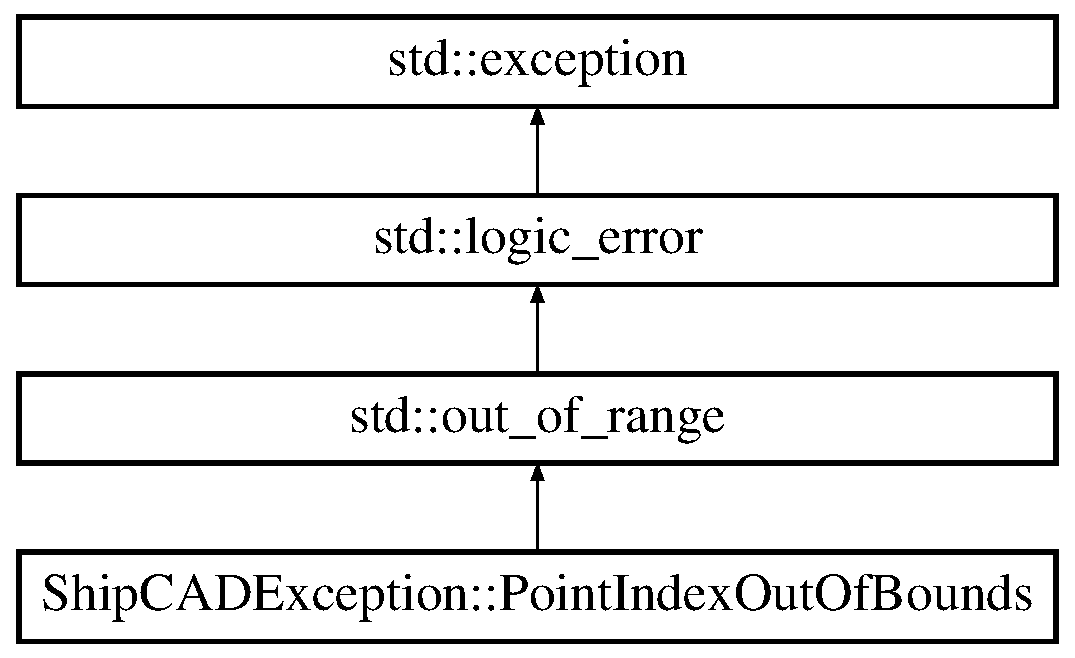
\includegraphics[height=4.000000cm]{classShipCADException_1_1PointIndexOutOfBounds}
\end{center}
\end{figure}
\subsection*{Public Member Functions}
\begin{DoxyCompactItemize}
\item 
\hyperlink{classShipCADException_1_1PointIndexOutOfBounds_aa9541484936b3d9fe243795cc9c03207}{Point\-Index\-Out\-Of\-Bounds} (const std\-::string \&what\-\_\-arg)
\end{DoxyCompactItemize}


\subsection{Detailed Description}


Definition at line 44 of file exception.\-h.



\subsection{Constructor \& Destructor Documentation}
\hypertarget{classShipCADException_1_1PointIndexOutOfBounds_aa9541484936b3d9fe243795cc9c03207}{\index{Ship\-C\-A\-D\-Exception\-::\-Point\-Index\-Out\-Of\-Bounds@{Ship\-C\-A\-D\-Exception\-::\-Point\-Index\-Out\-Of\-Bounds}!Point\-Index\-Out\-Of\-Bounds@{Point\-Index\-Out\-Of\-Bounds}}
\index{Point\-Index\-Out\-Of\-Bounds@{Point\-Index\-Out\-Of\-Bounds}!ShipCADException::PointIndexOutOfBounds@{Ship\-C\-A\-D\-Exception\-::\-Point\-Index\-Out\-Of\-Bounds}}
\subsubsection[{Point\-Index\-Out\-Of\-Bounds}]{\setlength{\rightskip}{0pt plus 5cm}Ship\-C\-A\-D\-Exception\-::\-Point\-Index\-Out\-Of\-Bounds\-::\-Point\-Index\-Out\-Of\-Bounds (
\begin{DoxyParamCaption}
\item[{const std\-::string \&}]{what\-\_\-arg}
\end{DoxyParamCaption}
)\hspace{0.3cm}{\ttfamily [inline]}}}\label{classShipCADException_1_1PointIndexOutOfBounds_aa9541484936b3d9fe243795cc9c03207}


Definition at line 47 of file exception.\-h.



The documentation for this class was generated from the following file\-:\begin{DoxyCompactItemize}
\item 
Ship\-C\-A\-Dlib/\hyperlink{exception_8h}{exception.\-h}\end{DoxyCompactItemize}

\hypertarget{structPointPred}{\section{Point\-Pred Struct Reference}
\label{structPointPred}\index{Point\-Pred@{Point\-Pred}}
}
\subsection*{Public Member Functions}
\begin{DoxyCompactItemize}
\item 
bool \hyperlink{structPointPred_a3e2cfa1956feb6ddc90b9e48e52a241f}{operator()} (const pair$<$ \hyperlink{classShipCADGeometry_1_1SubdivisionPoint}{Ship\-C\-A\-D\-Geometry\-::\-Subdivision\-Point} $\ast$, \hyperlink{classShipCADGeometry_1_1SubdivisionPoint}{Ship\-C\-A\-D\-Geometry\-::\-Subdivision\-Point} $\ast$ $>$ \&val)
\item 
\hyperlink{structPointPred_aebfb99e471eb88c6abb630b2b0886c49}{Point\-Pred} (\hyperlink{classShipCADGeometry_1_1SubdivisionPoint}{Ship\-C\-A\-D\-Geometry\-::\-Subdivision\-Point} $\ast$querypt)
\end{DoxyCompactItemize}
\subsection*{Public Attributes}
\begin{DoxyCompactItemize}
\item 
\hyperlink{classShipCADGeometry_1_1SubdivisionPoint}{Ship\-C\-A\-D\-Geometry\-::\-Subdivision\-Point} $\ast$ \hyperlink{structPointPred_a44ee45b04c1d27518a0da3c19591d4b0}{\-\_\-querypt}
\end{DoxyCompactItemize}


\subsection{Detailed Description}


Definition at line 224 of file subdivface.\-cpp.



\subsection{Constructor \& Destructor Documentation}
\hypertarget{structPointPred_aebfb99e471eb88c6abb630b2b0886c49}{\index{Point\-Pred@{Point\-Pred}!Point\-Pred@{Point\-Pred}}
\index{Point\-Pred@{Point\-Pred}!PointPred@{Point\-Pred}}
\subsubsection[{Point\-Pred}]{\setlength{\rightskip}{0pt plus 5cm}Point\-Pred\-::\-Point\-Pred (
\begin{DoxyParamCaption}
\item[{{\bf Ship\-C\-A\-D\-Geometry\-::\-Subdivision\-Point} $\ast$}]{querypt}
\end{DoxyParamCaption}
)\hspace{0.3cm}{\ttfamily [inline]}}}\label{structPointPred_aebfb99e471eb88c6abb630b2b0886c49}


Definition at line 230 of file subdivface.\-cpp.



\subsection{Member Function Documentation}
\hypertarget{structPointPred_a3e2cfa1956feb6ddc90b9e48e52a241f}{\index{Point\-Pred@{Point\-Pred}!operator()@{operator()}}
\index{operator()@{operator()}!PointPred@{Point\-Pred}}
\subsubsection[{operator()}]{\setlength{\rightskip}{0pt plus 5cm}bool Point\-Pred\-::operator() (
\begin{DoxyParamCaption}
\item[{const pair$<$ {\bf Ship\-C\-A\-D\-Geometry\-::\-Subdivision\-Point} $\ast$, {\bf Ship\-C\-A\-D\-Geometry\-::\-Subdivision\-Point} $\ast$ $>$ \&}]{val}
\end{DoxyParamCaption}
)\hspace{0.3cm}{\ttfamily [inline]}}}\label{structPointPred_a3e2cfa1956feb6ddc90b9e48e52a241f}


Definition at line 226 of file subdivface.\-cpp.



\subsection{Member Data Documentation}
\hypertarget{structPointPred_a44ee45b04c1d27518a0da3c19591d4b0}{\index{Point\-Pred@{Point\-Pred}!\-\_\-querypt@{\-\_\-querypt}}
\index{\-\_\-querypt@{\-\_\-querypt}!PointPred@{Point\-Pred}}
\subsubsection[{\-\_\-querypt}]{\setlength{\rightskip}{0pt plus 5cm}{\bf Ship\-C\-A\-D\-Geometry\-::\-Subdivision\-Point}$\ast$ Point\-Pred\-::\-\_\-querypt}}\label{structPointPred_a44ee45b04c1d27518a0da3c19591d4b0}


Definition at line 225 of file subdivface.\-cpp.



The documentation for this struct was generated from the following file\-:\begin{DoxyCompactItemize}
\item 
Ship\-C\-A\-Dlib/\hyperlink{subdivface_8cpp}{subdivface.\-cpp}\end{DoxyCompactItemize}

\hypertarget{classShipCADGeometry_1_1Shader}{\section{Ship\-C\-A\-D\-Geometry\-:\-:Shader Class Reference}
\label{classShipCADGeometry_1_1Shader}\index{Ship\-C\-A\-D\-Geometry\-::\-Shader@{Ship\-C\-A\-D\-Geometry\-::\-Shader}}
}


{\ttfamily \#include $<$shader.\-h$>$}

Inheritance diagram for Ship\-C\-A\-D\-Geometry\-:\-:Shader\-:\begin{figure}[H]
\begin{center}
\leavevmode
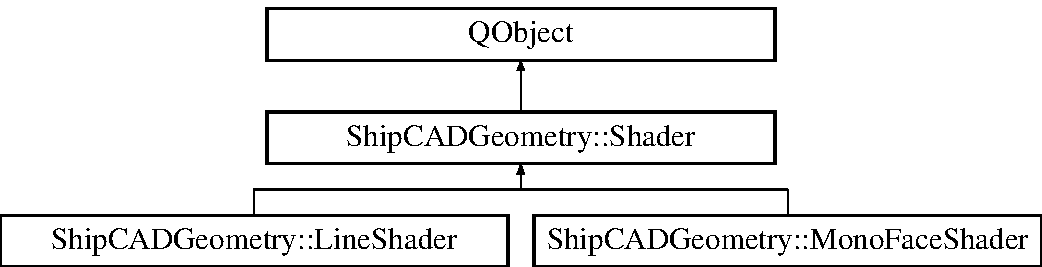
\includegraphics[height=3.000000cm]{classShipCADGeometry_1_1Shader}
\end{center}
\end{figure}
\subsection*{Public Member Functions}
\begin{DoxyCompactItemize}
\item 
\hyperlink{classShipCADGeometry_1_1Shader_a36bc24054e22fb965b04dae9a2b76eb7}{Shader} (\hyperlink{classShipCADGeometry_1_1Viewport}{Viewport} $\ast$vp)
\item 
virtual \hyperlink{classShipCADGeometry_1_1Shader_aff01df87e8a102f270b5b135a295e59d}{$\sim$\-Shader} ()
\item 
virtual void \hyperlink{classShipCADGeometry_1_1Shader_a011fae279e362f548e8c4e4b35b7291e}{initialize} (const char $\ast$vertex\-Shader\-Source, const char $\ast$fragment\-Shader\-Source, std\-::vector$<$ std\-::string $>$ uniforms, std\-::vector$<$ std\-::string $>$ attributes)
\item 
void \hyperlink{classShipCADGeometry_1_1Shader_ac8faec958f9d5806510d39be5f512c8e}{add\-Uniform} (const std\-::string \&name)
\item 
void \hyperlink{classShipCADGeometry_1_1Shader_a6a298be357d7860d859aedbe397b81b9}{add\-Attribute} (const std\-::string \&name)
\item 
void \hyperlink{classShipCADGeometry_1_1Shader_a7d7fe16e4eb06ad1eb19e22b38cff96e}{set\-Matrix} (const Q\-Matrix4x4 \&matrix)
\item 
void \hyperlink{classShipCADGeometry_1_1Shader_a29440ce9478af96ffae40b8928cc03f0}{bind} ()
\item 
void \hyperlink{classShipCADGeometry_1_1Shader_a2c7d1fca280aec57ba648ccdbdeed7a9}{release} ()
\end{DoxyCompactItemize}
\subsection*{Protected Attributes}
\begin{DoxyCompactItemize}
\item 
\hyperlink{classShipCADGeometry_1_1Viewport}{Viewport} $\ast$ \hyperlink{classShipCADGeometry_1_1Shader_a23ce29f9de114bcfe114028465c58136}{\-\_\-viewport}
\item 
Q\-Open\-G\-L\-Shader\-Program $\ast$ \hyperlink{classShipCADGeometry_1_1Shader_a1e25fa850e34b5f1f025e67a96c42349}{\-\_\-program}
\item 
std\-::map$<$ std\-::string, G\-Luint $>$ \hyperlink{classShipCADGeometry_1_1Shader_ab5999f6b8f8542413147444f5144d523}{\-\_\-uniforms}
\item 
std\-::map$<$ std\-::string, G\-Luint $>$ \hyperlink{classShipCADGeometry_1_1Shader_a0277ebbb9232cacd53738979f9a0b62e}{\-\_\-attributes}
\end{DoxyCompactItemize}


\subsection{Detailed Description}


Definition at line 45 of file shader.\-h.



\subsection{Constructor \& Destructor Documentation}
\hypertarget{classShipCADGeometry_1_1Shader_a36bc24054e22fb965b04dae9a2b76eb7}{\index{Ship\-C\-A\-D\-Geometry\-::\-Shader@{Ship\-C\-A\-D\-Geometry\-::\-Shader}!Shader@{Shader}}
\index{Shader@{Shader}!ShipCADGeometry::Shader@{Ship\-C\-A\-D\-Geometry\-::\-Shader}}
\subsubsection[{Shader}]{\setlength{\rightskip}{0pt plus 5cm}Shader\-::\-Shader (
\begin{DoxyParamCaption}
\item[{{\bf Viewport} $\ast$}]{vp}
\end{DoxyParamCaption}
)\hspace{0.3cm}{\ttfamily [explicit]}}}\label{classShipCADGeometry_1_1Shader_a36bc24054e22fb965b04dae9a2b76eb7}


Definition at line 42 of file shader.\-cpp.

\hypertarget{classShipCADGeometry_1_1Shader_aff01df87e8a102f270b5b135a295e59d}{\index{Ship\-C\-A\-D\-Geometry\-::\-Shader@{Ship\-C\-A\-D\-Geometry\-::\-Shader}!$\sim$\-Shader@{$\sim$\-Shader}}
\index{$\sim$\-Shader@{$\sim$\-Shader}!ShipCADGeometry::Shader@{Ship\-C\-A\-D\-Geometry\-::\-Shader}}
\subsubsection[{$\sim$\-Shader}]{\setlength{\rightskip}{0pt plus 5cm}Shader\-::$\sim$\-Shader (
\begin{DoxyParamCaption}
{}
\end{DoxyParamCaption}
)\hspace{0.3cm}{\ttfamily [virtual]}}}\label{classShipCADGeometry_1_1Shader_aff01df87e8a102f270b5b135a295e59d}


Definition at line 48 of file shader.\-cpp.



\subsection{Member Function Documentation}
\hypertarget{classShipCADGeometry_1_1Shader_a6a298be357d7860d859aedbe397b81b9}{\index{Ship\-C\-A\-D\-Geometry\-::\-Shader@{Ship\-C\-A\-D\-Geometry\-::\-Shader}!add\-Attribute@{add\-Attribute}}
\index{add\-Attribute@{add\-Attribute}!ShipCADGeometry::Shader@{Ship\-C\-A\-D\-Geometry\-::\-Shader}}
\subsubsection[{add\-Attribute}]{\setlength{\rightskip}{0pt plus 5cm}void Shader\-::add\-Attribute (
\begin{DoxyParamCaption}
\item[{const std\-::string \&}]{name}
\end{DoxyParamCaption}
)}}\label{classShipCADGeometry_1_1Shader_a6a298be357d7860d859aedbe397b81b9}


Definition at line 79 of file shader.\-cpp.

\hypertarget{classShipCADGeometry_1_1Shader_ac8faec958f9d5806510d39be5f512c8e}{\index{Ship\-C\-A\-D\-Geometry\-::\-Shader@{Ship\-C\-A\-D\-Geometry\-::\-Shader}!add\-Uniform@{add\-Uniform}}
\index{add\-Uniform@{add\-Uniform}!ShipCADGeometry::Shader@{Ship\-C\-A\-D\-Geometry\-::\-Shader}}
\subsubsection[{add\-Uniform}]{\setlength{\rightskip}{0pt plus 5cm}void Shader\-::add\-Uniform (
\begin{DoxyParamCaption}
\item[{const std\-::string \&}]{name}
\end{DoxyParamCaption}
)}}\label{classShipCADGeometry_1_1Shader_ac8faec958f9d5806510d39be5f512c8e}


Definition at line 72 of file shader.\-cpp.

\hypertarget{classShipCADGeometry_1_1Shader_a29440ce9478af96ffae40b8928cc03f0}{\index{Ship\-C\-A\-D\-Geometry\-::\-Shader@{Ship\-C\-A\-D\-Geometry\-::\-Shader}!bind@{bind}}
\index{bind@{bind}!ShipCADGeometry::Shader@{Ship\-C\-A\-D\-Geometry\-::\-Shader}}
\subsubsection[{bind}]{\setlength{\rightskip}{0pt plus 5cm}void Ship\-C\-A\-D\-Geometry\-::\-Shader\-::bind (
\begin{DoxyParamCaption}
{}
\end{DoxyParamCaption}
)\hspace{0.3cm}{\ttfamily [inline]}}}\label{classShipCADGeometry_1_1Shader_a29440ce9478af96ffae40b8928cc03f0}


Definition at line 64 of file shader.\-h.

\hypertarget{classShipCADGeometry_1_1Shader_a011fae279e362f548e8c4e4b35b7291e}{\index{Ship\-C\-A\-D\-Geometry\-::\-Shader@{Ship\-C\-A\-D\-Geometry\-::\-Shader}!initialize@{initialize}}
\index{initialize@{initialize}!ShipCADGeometry::Shader@{Ship\-C\-A\-D\-Geometry\-::\-Shader}}
\subsubsection[{initialize}]{\setlength{\rightskip}{0pt plus 5cm}void Shader\-::initialize (
\begin{DoxyParamCaption}
\item[{const char $\ast$}]{vertex\-Shader\-Source, }
\item[{const char $\ast$}]{fragment\-Shader\-Source, }
\item[{std\-::vector$<$ std\-::string $>$}]{uniforms, }
\item[{std\-::vector$<$ std\-::string $>$}]{attributes}
\end{DoxyParamCaption}
)\hspace{0.3cm}{\ttfamily [virtual]}}}\label{classShipCADGeometry_1_1Shader_a011fae279e362f548e8c4e4b35b7291e}


Definition at line 53 of file shader.\-cpp.

\hypertarget{classShipCADGeometry_1_1Shader_a2c7d1fca280aec57ba648ccdbdeed7a9}{\index{Ship\-C\-A\-D\-Geometry\-::\-Shader@{Ship\-C\-A\-D\-Geometry\-::\-Shader}!release@{release}}
\index{release@{release}!ShipCADGeometry::Shader@{Ship\-C\-A\-D\-Geometry\-::\-Shader}}
\subsubsection[{release}]{\setlength{\rightskip}{0pt plus 5cm}void Ship\-C\-A\-D\-Geometry\-::\-Shader\-::release (
\begin{DoxyParamCaption}
{}
\end{DoxyParamCaption}
)\hspace{0.3cm}{\ttfamily [inline]}}}\label{classShipCADGeometry_1_1Shader_a2c7d1fca280aec57ba648ccdbdeed7a9}


Definition at line 65 of file shader.\-h.

\hypertarget{classShipCADGeometry_1_1Shader_a7d7fe16e4eb06ad1eb19e22b38cff96e}{\index{Ship\-C\-A\-D\-Geometry\-::\-Shader@{Ship\-C\-A\-D\-Geometry\-::\-Shader}!set\-Matrix@{set\-Matrix}}
\index{set\-Matrix@{set\-Matrix}!ShipCADGeometry::Shader@{Ship\-C\-A\-D\-Geometry\-::\-Shader}}
\subsubsection[{set\-Matrix}]{\setlength{\rightskip}{0pt plus 5cm}void Shader\-::set\-Matrix (
\begin{DoxyParamCaption}
\item[{const Q\-Matrix4x4 \&}]{matrix}
\end{DoxyParamCaption}
)}}\label{classShipCADGeometry_1_1Shader_a7d7fe16e4eb06ad1eb19e22b38cff96e}


Definition at line 86 of file shader.\-cpp.



\subsection{Member Data Documentation}
\hypertarget{classShipCADGeometry_1_1Shader_a0277ebbb9232cacd53738979f9a0b62e}{\index{Ship\-C\-A\-D\-Geometry\-::\-Shader@{Ship\-C\-A\-D\-Geometry\-::\-Shader}!\-\_\-attributes@{\-\_\-attributes}}
\index{\-\_\-attributes@{\-\_\-attributes}!ShipCADGeometry::Shader@{Ship\-C\-A\-D\-Geometry\-::\-Shader}}
\subsubsection[{\-\_\-attributes}]{\setlength{\rightskip}{0pt plus 5cm}std\-::map$<$std\-::string, G\-Luint$>$ Ship\-C\-A\-D\-Geometry\-::\-Shader\-::\-\_\-attributes\hspace{0.3cm}{\ttfamily [protected]}}}\label{classShipCADGeometry_1_1Shader_a0277ebbb9232cacd53738979f9a0b62e}


Definition at line 72 of file shader.\-h.

\hypertarget{classShipCADGeometry_1_1Shader_a1e25fa850e34b5f1f025e67a96c42349}{\index{Ship\-C\-A\-D\-Geometry\-::\-Shader@{Ship\-C\-A\-D\-Geometry\-::\-Shader}!\-\_\-program@{\-\_\-program}}
\index{\-\_\-program@{\-\_\-program}!ShipCADGeometry::Shader@{Ship\-C\-A\-D\-Geometry\-::\-Shader}}
\subsubsection[{\-\_\-program}]{\setlength{\rightskip}{0pt plus 5cm}Q\-Open\-G\-L\-Shader\-Program$\ast$ Ship\-C\-A\-D\-Geometry\-::\-Shader\-::\-\_\-program\hspace{0.3cm}{\ttfamily [protected]}}}\label{classShipCADGeometry_1_1Shader_a1e25fa850e34b5f1f025e67a96c42349}


Definition at line 70 of file shader.\-h.

\hypertarget{classShipCADGeometry_1_1Shader_ab5999f6b8f8542413147444f5144d523}{\index{Ship\-C\-A\-D\-Geometry\-::\-Shader@{Ship\-C\-A\-D\-Geometry\-::\-Shader}!\-\_\-uniforms@{\-\_\-uniforms}}
\index{\-\_\-uniforms@{\-\_\-uniforms}!ShipCADGeometry::Shader@{Ship\-C\-A\-D\-Geometry\-::\-Shader}}
\subsubsection[{\-\_\-uniforms}]{\setlength{\rightskip}{0pt plus 5cm}std\-::map$<$std\-::string, G\-Luint$>$ Ship\-C\-A\-D\-Geometry\-::\-Shader\-::\-\_\-uniforms\hspace{0.3cm}{\ttfamily [protected]}}}\label{classShipCADGeometry_1_1Shader_ab5999f6b8f8542413147444f5144d523}


Definition at line 71 of file shader.\-h.

\hypertarget{classShipCADGeometry_1_1Shader_a23ce29f9de114bcfe114028465c58136}{\index{Ship\-C\-A\-D\-Geometry\-::\-Shader@{Ship\-C\-A\-D\-Geometry\-::\-Shader}!\-\_\-viewport@{\-\_\-viewport}}
\index{\-\_\-viewport@{\-\_\-viewport}!ShipCADGeometry::Shader@{Ship\-C\-A\-D\-Geometry\-::\-Shader}}
\subsubsection[{\-\_\-viewport}]{\setlength{\rightskip}{0pt plus 5cm}{\bf Viewport}$\ast$ Ship\-C\-A\-D\-Geometry\-::\-Shader\-::\-\_\-viewport\hspace{0.3cm}{\ttfamily [protected]}}}\label{classShipCADGeometry_1_1Shader_a23ce29f9de114bcfe114028465c58136}


Definition at line 69 of file shader.\-h.



The documentation for this class was generated from the following files\-:\begin{DoxyCompactItemize}
\item 
Ship\-C\-A\-Dlib/\hyperlink{shader_8h}{shader.\-h}\item 
Ship\-C\-A\-Dlib/\hyperlink{shader_8cpp}{shader.\-cpp}\end{DoxyCompactItemize}

\hypertarget{classShipCADlib}{\section{Ship\-C\-A\-Dlib Class Reference}
\label{classShipCADlib}\index{Ship\-C\-A\-Dlib@{Ship\-C\-A\-Dlib}}
}


{\ttfamily \#include $<$shipcadlib.\-h$>$}

\subsection*{Public Member Functions}
\begin{DoxyCompactItemize}
\item 
\hyperlink{classShipCADlib_a836f353d6883b0dc662ccd36e00efb8f}{Ship\-C\-A\-Dlib} ()
\end{DoxyCompactItemize}


\subsection{Detailed Description}


Definition at line 34 of file shipcadlib.\-h.



\subsection{Constructor \& Destructor Documentation}
\hypertarget{classShipCADlib_a836f353d6883b0dc662ccd36e00efb8f}{\index{Ship\-C\-A\-Dlib@{Ship\-C\-A\-Dlib}!Ship\-C\-A\-Dlib@{Ship\-C\-A\-Dlib}}
\index{Ship\-C\-A\-Dlib@{Ship\-C\-A\-Dlib}!ShipCADlib@{Ship\-C\-A\-Dlib}}
\subsubsection[{Ship\-C\-A\-Dlib}]{\setlength{\rightskip}{0pt plus 5cm}Ship\-C\-A\-Dlib\-::\-Ship\-C\-A\-Dlib (
\begin{DoxyParamCaption}
{}
\end{DoxyParamCaption}
)}}\label{classShipCADlib_a836f353d6883b0dc662ccd36e00efb8f}


Definition at line 33 of file shipcadlib.\-cpp.



The documentation for this class was generated from the following files\-:\begin{DoxyCompactItemize}
\item 
Ship\-C\-A\-Dlib/\hyperlink{shipcadlib_8h}{shipcadlib.\-h}\item 
Ship\-C\-A\-Dlib/\hyperlink{shipcadlib_8cpp}{shipcadlib.\-cpp}\end{DoxyCompactItemize}

\hypertarget{classShipCADGeometry_1_1Spline}{\section{Ship\-C\-A\-D\-Geometry\-:\-:Spline Class Reference}
\label{classShipCADGeometry_1_1Spline}\index{Ship\-C\-A\-D\-Geometry\-::\-Spline@{Ship\-C\-A\-D\-Geometry\-::\-Spline}}
}


{\ttfamily \#include $<$spline.\-h$>$}

Inheritance diagram for Ship\-C\-A\-D\-Geometry\-:\-:Spline\-:\begin{figure}[H]
\begin{center}
\leavevmode
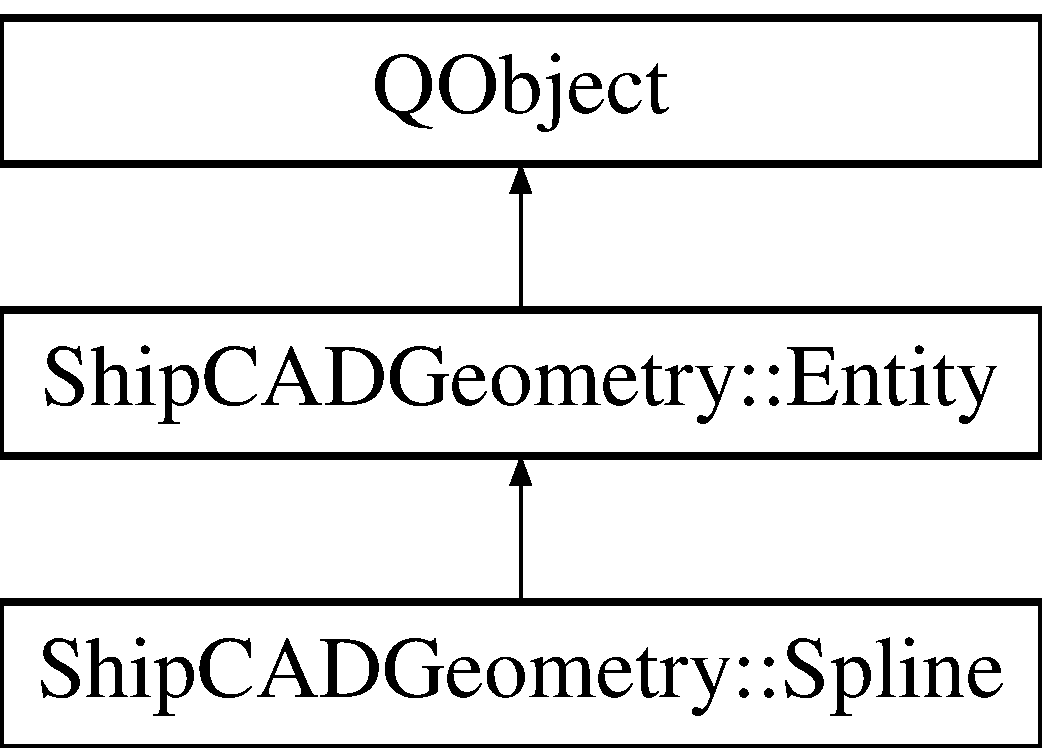
\includegraphics[height=3.000000cm]{classShipCADGeometry_1_1Spline}
\end{center}
\end{figure}
\subsection*{Public Member Functions}
\begin{DoxyCompactItemize}
\item 
\hyperlink{classShipCADGeometry_1_1Spline_a7ad84ea604562c7c9cb309b4e78e25c5}{Spline} ()
\item 
virtual \hyperlink{classShipCADGeometry_1_1Spline_a0c900ca3c99987532e1d0c21ba992968}{$\sim$\-Spline} ()
\item 
void \hyperlink{classShipCADGeometry_1_1Spline_ac3d9f4514573be91b316413bf062791a}{add} (const Q\-Vector3\-D \&p)
\item 
void \hyperlink{classShipCADGeometry_1_1Spline_a120c5530571f138daad61426053220f3}{delete\-\_\-point} (size\-\_\-t index)
\item 
void \hyperlink{classShipCADGeometry_1_1Spline_aa1ea6446e0b59d5cce88580242cd25b6}{insert} (size\-\_\-t index, const Q\-Vector3\-D \&p)
\item 
void \hyperlink{classShipCADGeometry_1_1Spline_aa8e588b92d23c74bb6ec120624b49e54}{insert\-\_\-spline} (size\-\_\-t index, bool invert, bool duplicate\-\_\-point, const \hyperlink{classShipCADGeometry_1_1Spline}{Spline} \&source)
\item 
void \hyperlink{classShipCADGeometry_1_1Spline_a26293a4ee636c2b968c45731425d5c94}{invert\-\_\-direction} ()
\item 
bool \hyperlink{classShipCADGeometry_1_1Spline_a043f418b363a0dc7161b9106a72ef8b4}{simplify} (float criterium)
\item 
virtual void \hyperlink{classShipCADGeometry_1_1Spline_a02967f3eee8b1755eab0d7da55c3c621}{clear} ()
\item 
virtual void \hyperlink{classShipCADGeometry_1_1Spline_a9b466ad7510032dafb0421f2d834bde6}{rebuild} ()
\item 
float \hyperlink{classShipCADGeometry_1_1Spline_a9d4d64a34b1511efc5c41b9e31956a3e}{coord\-\_\-length} (float t1, float t2)
\item 
float \hyperlink{classShipCADGeometry_1_1Spline_ae15513771d88f4f545048d4204e98325}{chord\-\_\-length\-\_\-approximation} (float percentage)
\item 
float \hyperlink{classShipCADGeometry_1_1Spline_a5681a27480f934a73462e53b2b4e2461}{curvature} (float parameter, Q\-Vector3\-D \&normal)
\item 
Q\-Vector3\-D \hyperlink{classShipCADGeometry_1_1Spline_afe15664ac97d1d3452d5a5cfd023c471}{first\-\_\-derive} (float parameter)
\item 
Q\-Vector3\-D \hyperlink{classShipCADGeometry_1_1Spline_abe04c117432e350f3a9f66395d2d3037}{second\-\_\-derive} (float parameter)
\item 
bool \hyperlink{classShipCADGeometry_1_1Spline_afd932e0c63a3b03200ecdc7c656be8e4}{intersect\-\_\-plane} (const \hyperlink{classShipCADGeometry_1_1Plane}{Plane} \&plane, \hyperlink{classShipCADGeometry_1_1IntersectionData}{Intersection\-Data} \&output)
\item 
Q\-Vector3\-D \hyperlink{classShipCADGeometry_1_1Spline_a589d6d945e0fbb905ea94907cd216165}{value} (float parameter)
\item 
virtual void \hyperlink{classShipCADGeometry_1_1Spline_aedf951fc91bb7465959ea8dc23356cdd}{load\-\_\-binary} (\hyperlink{classShipCADGeometry_1_1FileBuffer}{File\-Buffer} \&source)
\item 
virtual void \hyperlink{classShipCADGeometry_1_1Spline_aa353db49887868aa708c310aec3537f5}{save\-\_\-binary} (\hyperlink{classShipCADGeometry_1_1FileBuffer}{File\-Buffer} \&destination)
\item 
void \hyperlink{classShipCADGeometry_1_1Spline_a8b50b6f5338b9504bd6850a605b53620}{save\-\_\-to\-\_\-dxf} (std\-::vector$<$ Q\-String $>$ \&strings, Q\-String layername, bool sendmirror)
\item 
virtual void \hyperlink{classShipCADGeometry_1_1Spline_a6424ed433d241f566c15891cc25a74dd}{draw} (\hyperlink{classShipCADGeometry_1_1Viewport}{Viewport} \&vp, \hyperlink{classShipCADGeometry_1_1LineShader}{Line\-Shader} $\ast$lineshader)
\item 
bool \hyperlink{classShipCADGeometry_1_1Spline_a15d2f95f885223099dbd2f04b43f05c9}{show\-Curvature} ()
\item 
void \hyperlink{classShipCADGeometry_1_1Spline_a2d38ce18032601fb8e94d8b0368b3954}{set\-Show\-Curvature} (bool val)
\item 
Q\-Color \hyperlink{classShipCADGeometry_1_1Spline_a9a6c37e20ea46497a2e5a8274f55514e}{get\-Curvature\-Color} ()
\item 
void \hyperlink{classShipCADGeometry_1_1Spline_a8ac4a4b3e3da9282d7b470e3937cb1e5}{set\-Curvature\-Color} (const Q\-Color \&val)
\item 
float \hyperlink{classShipCADGeometry_1_1Spline_a8af6aa0b0c11d98dfabb72f594c30151}{get\-Curvature\-Scale} ()
\item 
void \hyperlink{classShipCADGeometry_1_1Spline_a7e205cdf485b5b7c5ab7d436ea097fed}{set\-Curvature\-Scale} (float val)
\item 
float \hyperlink{classShipCADGeometry_1_1Spline_ac617856776bb267bdab050b56de4ec74}{get\-Parameter} (size\-\_\-t index)
\item 
Q\-Vector3\-D \hyperlink{classShipCADGeometry_1_1Spline_ad316be28cfd23e518f9e761c46644440}{get\-Point} (size\-\_\-t index)
\item 
void \hyperlink{classShipCADGeometry_1_1Spline_ae02af8d5473f952644ac5103d7beebf2}{set\-Point} (size\-\_\-t index, const Q\-Vector3\-D \&p)
\item 
int \hyperlink{classShipCADGeometry_1_1Spline_a489b034b416be54fe323ad021620f820}{get\-Fragments} ()
\item 
void \hyperlink{classShipCADGeometry_1_1Spline_aaae6e558fad0833cde71f9ed38e4fb96}{set\-Fragments} (size\-\_\-t val)
\item 
bool \hyperlink{classShipCADGeometry_1_1Spline_a90a954f52321f3b1b27b43991e9997a5}{is\-Knuckle} (size\-\_\-t index)
\item 
void \hyperlink{classShipCADGeometry_1_1Spline_ad4f075e2e8f1d3ac7c2d22b5be75bbad}{set\-Knuckle} (size\-\_\-t index, bool val)
\item 
size\-\_\-t \hyperlink{classShipCADGeometry_1_1Spline_a4f040e953d07359616c9342f2aff0029}{number\-Of\-Points} ()
\item 
void \hyperlink{classShipCADGeometry_1_1Spline_a156ffe855d149ad445b178078ee4451c}{dump} (std\-::ostream \&os) const 
\end{DoxyCompactItemize}
\subsection*{Protected Member Functions}
\begin{DoxyCompactItemize}
\item 
void \hyperlink{classShipCADGeometry_1_1Spline_a6e932411f0f4463514f80011c58f5e6a}{set\-Build} (bool val)
\item 
float \hyperlink{classShipCADGeometry_1_1Spline_a63165f7cf70338e51b0f16504366031e}{weight} (size\-\_\-t index)
\item 
std\-::vector$<$ float $>$\-::iterator \hyperlink{classShipCADGeometry_1_1Spline_a20b39f3a1bd853040df4760cd912ee64}{find\-\_\-next\-\_\-point} (std\-::vector$<$ float $>$ \&weights)
\item 
void \hyperlink{classShipCADGeometry_1_1Spline_ab8f0b98595ccbd62e754fe92354a207b}{add\-\_\-to\-\_\-output} (const Q\-Vector3\-D \&p, float parameter, \hyperlink{classShipCADGeometry_1_1IntersectionData}{Intersection\-Data} \&output)
\end{DoxyCompactItemize}
\subsection*{Protected Attributes}
\begin{DoxyCompactItemize}
\item 
size\-\_\-t \hyperlink{classShipCADGeometry_1_1Spline_a0d0c8014132eda7835842d6a20ccdf74}{\-\_\-nopoints}
\item 
size\-\_\-t \hyperlink{classShipCADGeometry_1_1Spline_afc73aefcc80c61121888a63abf687b40}{\-\_\-fragments}
\item 
bool \hyperlink{classShipCADGeometry_1_1Spline_aa3640f8d0561a651aec79a5d80c871f3}{\-\_\-show\-\_\-curvature}
\item 
bool \hyperlink{classShipCADGeometry_1_1Spline_a64b335f1c21a26f5f01ddcfbf92501d6}{\-\_\-show\-\_\-points}
\item 
float \hyperlink{classShipCADGeometry_1_1Spline_a775e87cfe42d7f2eb747b1ab3e772b88}{\-\_\-curvature\-\_\-scale}
\item 
Q\-Color \hyperlink{classShipCADGeometry_1_1Spline_a2c51c87d9f9caedf39f887029f040a36}{\-\_\-curvature\-\_\-color}
\item 
std\-::vector$<$ Q\-Vector3\-D $>$ \hyperlink{classShipCADGeometry_1_1Spline_ab6db595e6a4dd703838d5baec8543f34}{\-\_\-points}
\item 
std\-::vector$<$ bool $>$ \hyperlink{classShipCADGeometry_1_1Spline_a5bfae9fec6fa04634083bb7fa6ac9452}{\-\_\-knuckles}
\item 
float \hyperlink{classShipCADGeometry_1_1Spline_a4f4832362958e63f9b9503414466a2ae}{\-\_\-total\-\_\-length}
\item 
std\-::vector$<$ float $>$ \hyperlink{classShipCADGeometry_1_1Spline_a48f36b8eb159586aa334877f4ab7a015}{\-\_\-parameters}
\item 
std\-::vector$<$ Q\-Vector3\-D $>$ \hyperlink{classShipCADGeometry_1_1Spline_a57c78404d9c30c448d9f5ac377fc0e8f}{\-\_\-derivatives}
\end{DoxyCompactItemize}
\subsection*{Properties}
\begin{DoxyCompactItemize}
\item 
size\-\_\-t \hyperlink{classShipCADGeometry_1_1Spline_a964d9e0dcb98962d920dd5e595598a42}{Fragments}
\item 
bool \hyperlink{classShipCADGeometry_1_1Spline_ad4357d84fc550cf73581a303f7bd9088}{Show\-Curvature}
\item 
bool \hyperlink{classShipCADGeometry_1_1Spline_a7e14387674284ab28e1a0e725c5c5b0e}{Show\-Points}
\item 
float \hyperlink{classShipCADGeometry_1_1Spline_a2f9eb570f1bfe818d966a40cd0733df2}{Curvature\-Scale}
\item 
Q\-Color \hyperlink{classShipCADGeometry_1_1Spline_a4bc6d35c4d11b8df95e69300ef7120c7}{Curvature\-Color}
\end{DoxyCompactItemize}


\subsection{Detailed Description}


Definition at line 50 of file spline.\-h.



\subsection{Constructor \& Destructor Documentation}
\hypertarget{classShipCADGeometry_1_1Spline_a7ad84ea604562c7c9cb309b4e78e25c5}{\index{Ship\-C\-A\-D\-Geometry\-::\-Spline@{Ship\-C\-A\-D\-Geometry\-::\-Spline}!Spline@{Spline}}
\index{Spline@{Spline}!ShipCADGeometry::Spline@{Ship\-C\-A\-D\-Geometry\-::\-Spline}}
\subsubsection[{Spline}]{\setlength{\rightskip}{0pt plus 5cm}Spline\-::\-Spline (
\begin{DoxyParamCaption}
{}
\end{DoxyParamCaption}
)\hspace{0.3cm}{\ttfamily [explicit]}}}\label{classShipCADGeometry_1_1Spline_a7ad84ea604562c7c9cb309b4e78e25c5}


Definition at line 52 of file spline.\-cpp.

\hypertarget{classShipCADGeometry_1_1Spline_a0c900ca3c99987532e1d0c21ba992968}{\index{Ship\-C\-A\-D\-Geometry\-::\-Spline@{Ship\-C\-A\-D\-Geometry\-::\-Spline}!$\sim$\-Spline@{$\sim$\-Spline}}
\index{$\sim$\-Spline@{$\sim$\-Spline}!ShipCADGeometry::Spline@{Ship\-C\-A\-D\-Geometry\-::\-Spline}}
\subsubsection[{$\sim$\-Spline}]{\setlength{\rightskip}{0pt plus 5cm}Spline\-::$\sim$\-Spline (
\begin{DoxyParamCaption}
{}
\end{DoxyParamCaption}
)\hspace{0.3cm}{\ttfamily [virtual]}}}\label{classShipCADGeometry_1_1Spline_a0c900ca3c99987532e1d0c21ba992968}


Definition at line 58 of file spline.\-cpp.



\subsection{Member Function Documentation}
\hypertarget{classShipCADGeometry_1_1Spline_ac3d9f4514573be91b316413bf062791a}{\index{Ship\-C\-A\-D\-Geometry\-::\-Spline@{Ship\-C\-A\-D\-Geometry\-::\-Spline}!add@{add}}
\index{add@{add}!ShipCADGeometry::Spline@{Ship\-C\-A\-D\-Geometry\-::\-Spline}}
\subsubsection[{add}]{\setlength{\rightskip}{0pt plus 5cm}void Spline\-::add (
\begin{DoxyParamCaption}
\item[{const Q\-Vector3\-D \&}]{p}
\end{DoxyParamCaption}
)}}\label{classShipCADGeometry_1_1Spline_ac3d9f4514573be91b316413bf062791a}


Definition at line 389 of file spline.\-cpp.

\hypertarget{classShipCADGeometry_1_1Spline_ab8f0b98595ccbd62e754fe92354a207b}{\index{Ship\-C\-A\-D\-Geometry\-::\-Spline@{Ship\-C\-A\-D\-Geometry\-::\-Spline}!add\-\_\-to\-\_\-output@{add\-\_\-to\-\_\-output}}
\index{add\-\_\-to\-\_\-output@{add\-\_\-to\-\_\-output}!ShipCADGeometry::Spline@{Ship\-C\-A\-D\-Geometry\-::\-Spline}}
\subsubsection[{add\-\_\-to\-\_\-output}]{\setlength{\rightskip}{0pt plus 5cm}void Spline\-::add\-\_\-to\-\_\-output (
\begin{DoxyParamCaption}
\item[{const Q\-Vector3\-D \&}]{p, }
\item[{float}]{parameter, }
\item[{{\bf Intersection\-Data} \&}]{output}
\end{DoxyParamCaption}
)\hspace{0.3cm}{\ttfamily [protected]}}}\label{classShipCADGeometry_1_1Spline_ab8f0b98595ccbd62e754fe92354a207b}


Definition at line 610 of file spline.\-cpp.

\hypertarget{classShipCADGeometry_1_1Spline_ae15513771d88f4f545048d4204e98325}{\index{Ship\-C\-A\-D\-Geometry\-::\-Spline@{Ship\-C\-A\-D\-Geometry\-::\-Spline}!chord\-\_\-length\-\_\-approximation@{chord\-\_\-length\-\_\-approximation}}
\index{chord\-\_\-length\-\_\-approximation@{chord\-\_\-length\-\_\-approximation}!ShipCADGeometry::Spline@{Ship\-C\-A\-D\-Geometry\-::\-Spline}}
\subsubsection[{chord\-\_\-length\-\_\-approximation}]{\setlength{\rightskip}{0pt plus 5cm}float Spline\-::chord\-\_\-length\-\_\-approximation (
\begin{DoxyParamCaption}
\item[{float}]{percentage}
\end{DoxyParamCaption}
)}}\label{classShipCADGeometry_1_1Spline_ae15513771d88f4f545048d4204e98325}


Definition at line 417 of file spline.\-cpp.

\hypertarget{classShipCADGeometry_1_1Spline_a02967f3eee8b1755eab0d7da55c3c621}{\index{Ship\-C\-A\-D\-Geometry\-::\-Spline@{Ship\-C\-A\-D\-Geometry\-::\-Spline}!clear@{clear}}
\index{clear@{clear}!ShipCADGeometry::Spline@{Ship\-C\-A\-D\-Geometry\-::\-Spline}}
\subsubsection[{clear}]{\setlength{\rightskip}{0pt plus 5cm}void Spline\-::clear (
\begin{DoxyParamCaption}
{}
\end{DoxyParamCaption}
)\hspace{0.3cm}{\ttfamily [virtual]}}}\label{classShipCADGeometry_1_1Spline_a02967f3eee8b1755eab0d7da55c3c621}


Reimplemented from \hyperlink{classShipCADGeometry_1_1Entity_a998d0e5d360371046fd5835ba1e0877a}{Ship\-C\-A\-D\-Geometry\-::\-Entity}.



Definition at line 732 of file spline.\-cpp.

\hypertarget{classShipCADGeometry_1_1Spline_a9d4d64a34b1511efc5c41b9e31956a3e}{\index{Ship\-C\-A\-D\-Geometry\-::\-Spline@{Ship\-C\-A\-D\-Geometry\-::\-Spline}!coord\-\_\-length@{coord\-\_\-length}}
\index{coord\-\_\-length@{coord\-\_\-length}!ShipCADGeometry::Spline@{Ship\-C\-A\-D\-Geometry\-::\-Spline}}
\subsubsection[{coord\-\_\-length}]{\setlength{\rightskip}{0pt plus 5cm}float Spline\-::coord\-\_\-length (
\begin{DoxyParamCaption}
\item[{float}]{t1, }
\item[{float}]{t2}
\end{DoxyParamCaption}
)}}\label{classShipCADGeometry_1_1Spline_a9d4d64a34b1511efc5c41b9e31956a3e}


Definition at line 397 of file spline.\-cpp.

\hypertarget{classShipCADGeometry_1_1Spline_a5681a27480f934a73462e53b2b4e2461}{\index{Ship\-C\-A\-D\-Geometry\-::\-Spline@{Ship\-C\-A\-D\-Geometry\-::\-Spline}!curvature@{curvature}}
\index{curvature@{curvature}!ShipCADGeometry::Spline@{Ship\-C\-A\-D\-Geometry\-::\-Spline}}
\subsubsection[{curvature}]{\setlength{\rightskip}{0pt plus 5cm}float Spline\-::curvature (
\begin{DoxyParamCaption}
\item[{float}]{parameter, }
\item[{Q\-Vector3\-D \&}]{normal}
\end{DoxyParamCaption}
)}}\label{classShipCADGeometry_1_1Spline_a5681a27480f934a73462e53b2b4e2461}


Definition at line 465 of file spline.\-cpp.

\hypertarget{classShipCADGeometry_1_1Spline_a120c5530571f138daad61426053220f3}{\index{Ship\-C\-A\-D\-Geometry\-::\-Spline@{Ship\-C\-A\-D\-Geometry\-::\-Spline}!delete\-\_\-point@{delete\-\_\-point}}
\index{delete\-\_\-point@{delete\-\_\-point}!ShipCADGeometry::Spline@{Ship\-C\-A\-D\-Geometry\-::\-Spline}}
\subsubsection[{delete\-\_\-point}]{\setlength{\rightskip}{0pt plus 5cm}void Spline\-::delete\-\_\-point (
\begin{DoxyParamCaption}
\item[{size\-\_\-t}]{index}
\end{DoxyParamCaption}
)}}\label{classShipCADGeometry_1_1Spline_a120c5530571f138daad61426053220f3}


Definition at line 487 of file spline.\-cpp.

\hypertarget{classShipCADGeometry_1_1Spline_a6424ed433d241f566c15891cc25a74dd}{\index{Ship\-C\-A\-D\-Geometry\-::\-Spline@{Ship\-C\-A\-D\-Geometry\-::\-Spline}!draw@{draw}}
\index{draw@{draw}!ShipCADGeometry::Spline@{Ship\-C\-A\-D\-Geometry\-::\-Spline}}
\subsubsection[{draw}]{\setlength{\rightskip}{0pt plus 5cm}void Spline\-::draw (
\begin{DoxyParamCaption}
\item[{{\bf Viewport} \&}]{vp, }
\item[{{\bf Line\-Shader} $\ast$}]{lineshader}
\end{DoxyParamCaption}
)\hspace{0.3cm}{\ttfamily [virtual]}}}\label{classShipCADGeometry_1_1Spline_a6424ed433d241f566c15891cc25a74dd}


Implements \hyperlink{classShipCADGeometry_1_1Entity_a894bb00b5f65692c1a64e62d748f4041}{Ship\-C\-A\-D\-Geometry\-::\-Entity}.



Definition at line 525 of file spline.\-cpp.

\hypertarget{classShipCADGeometry_1_1Spline_a156ffe855d149ad445b178078ee4451c}{\index{Ship\-C\-A\-D\-Geometry\-::\-Spline@{Ship\-C\-A\-D\-Geometry\-::\-Spline}!dump@{dump}}
\index{dump@{dump}!ShipCADGeometry::Spline@{Ship\-C\-A\-D\-Geometry\-::\-Spline}}
\subsubsection[{dump}]{\setlength{\rightskip}{0pt plus 5cm}void Spline\-::dump (
\begin{DoxyParamCaption}
\item[{std\-::ostream \&}]{os}
\end{DoxyParamCaption}
) const}}\label{classShipCADGeometry_1_1Spline_a156ffe855d149ad445b178078ee4451c}


Definition at line 791 of file spline.\-cpp.

\hypertarget{classShipCADGeometry_1_1Spline_a20b39f3a1bd853040df4760cd912ee64}{\index{Ship\-C\-A\-D\-Geometry\-::\-Spline@{Ship\-C\-A\-D\-Geometry\-::\-Spline}!find\-\_\-next\-\_\-point@{find\-\_\-next\-\_\-point}}
\index{find\-\_\-next\-\_\-point@{find\-\_\-next\-\_\-point}!ShipCADGeometry::Spline@{Ship\-C\-A\-D\-Geometry\-::\-Spline}}
\subsubsection[{find\-\_\-next\-\_\-point}]{\setlength{\rightskip}{0pt plus 5cm}vector$<$ float $>$\-::iterator Spline\-::find\-\_\-next\-\_\-point (
\begin{DoxyParamCaption}
\item[{std\-::vector$<$ float $>$ \&}]{weights}
\end{DoxyParamCaption}
)\hspace{0.3cm}{\ttfamily [protected]}}}\label{classShipCADGeometry_1_1Spline_a20b39f3a1bd853040df4760cd912ee64}


Definition at line 326 of file spline.\-cpp.

\hypertarget{classShipCADGeometry_1_1Spline_afe15664ac97d1d3452d5a5cfd023c471}{\index{Ship\-C\-A\-D\-Geometry\-::\-Spline@{Ship\-C\-A\-D\-Geometry\-::\-Spline}!first\-\_\-derive@{first\-\_\-derive}}
\index{first\-\_\-derive@{first\-\_\-derive}!ShipCADGeometry::Spline@{Ship\-C\-A\-D\-Geometry\-::\-Spline}}
\subsubsection[{first\-\_\-derive}]{\setlength{\rightskip}{0pt plus 5cm}Q\-Vector3\-D Spline\-::first\-\_\-derive (
\begin{DoxyParamCaption}
\item[{float}]{parameter}
\end{DoxyParamCaption}
)}}\label{classShipCADGeometry_1_1Spline_afe15664ac97d1d3452d5a5cfd023c471}


Definition at line 497 of file spline.\-cpp.

\hypertarget{classShipCADGeometry_1_1Spline_a9a6c37e20ea46497a2e5a8274f55514e}{\index{Ship\-C\-A\-D\-Geometry\-::\-Spline@{Ship\-C\-A\-D\-Geometry\-::\-Spline}!get\-Curvature\-Color@{get\-Curvature\-Color}}
\index{get\-Curvature\-Color@{get\-Curvature\-Color}!ShipCADGeometry::Spline@{Ship\-C\-A\-D\-Geometry\-::\-Spline}}
\subsubsection[{get\-Curvature\-Color}]{\setlength{\rightskip}{0pt plus 5cm}Q\-Color Ship\-C\-A\-D\-Geometry\-::\-Spline\-::get\-Curvature\-Color (
\begin{DoxyParamCaption}
{}
\end{DoxyParamCaption}
)\hspace{0.3cm}{\ttfamily [inline]}}}\label{classShipCADGeometry_1_1Spline_a9a6c37e20ea46497a2e5a8274f55514e}


Definition at line 98 of file spline.\-h.

\hypertarget{classShipCADGeometry_1_1Spline_a8af6aa0b0c11d98dfabb72f594c30151}{\index{Ship\-C\-A\-D\-Geometry\-::\-Spline@{Ship\-C\-A\-D\-Geometry\-::\-Spline}!get\-Curvature\-Scale@{get\-Curvature\-Scale}}
\index{get\-Curvature\-Scale@{get\-Curvature\-Scale}!ShipCADGeometry::Spline@{Ship\-C\-A\-D\-Geometry\-::\-Spline}}
\subsubsection[{get\-Curvature\-Scale}]{\setlength{\rightskip}{0pt plus 5cm}float Ship\-C\-A\-D\-Geometry\-::\-Spline\-::get\-Curvature\-Scale (
\begin{DoxyParamCaption}
{}
\end{DoxyParamCaption}
)\hspace{0.3cm}{\ttfamily [inline]}}}\label{classShipCADGeometry_1_1Spline_a8af6aa0b0c11d98dfabb72f594c30151}


Definition at line 100 of file spline.\-h.

\hypertarget{classShipCADGeometry_1_1Spline_a489b034b416be54fe323ad021620f820}{\index{Ship\-C\-A\-D\-Geometry\-::\-Spline@{Ship\-C\-A\-D\-Geometry\-::\-Spline}!get\-Fragments@{get\-Fragments}}
\index{get\-Fragments@{get\-Fragments}!ShipCADGeometry::Spline@{Ship\-C\-A\-D\-Geometry\-::\-Spline}}
\subsubsection[{get\-Fragments}]{\setlength{\rightskip}{0pt plus 5cm}int Spline\-::get\-Fragments (
\begin{DoxyParamCaption}
{}
\end{DoxyParamCaption}
)}}\label{classShipCADGeometry_1_1Spline_a489b034b416be54fe323ad021620f820}


Definition at line 83 of file spline.\-cpp.

\hypertarget{classShipCADGeometry_1_1Spline_ac617856776bb267bdab050b56de4ec74}{\index{Ship\-C\-A\-D\-Geometry\-::\-Spline@{Ship\-C\-A\-D\-Geometry\-::\-Spline}!get\-Parameter@{get\-Parameter}}
\index{get\-Parameter@{get\-Parameter}!ShipCADGeometry::Spline@{Ship\-C\-A\-D\-Geometry\-::\-Spline}}
\subsubsection[{get\-Parameter}]{\setlength{\rightskip}{0pt plus 5cm}float Spline\-::get\-Parameter (
\begin{DoxyParamCaption}
\item[{size\-\_\-t}]{index}
\end{DoxyParamCaption}
)}}\label{classShipCADGeometry_1_1Spline_ac617856776bb267bdab050b56de4ec74}


Definition at line 117 of file spline.\-cpp.

\hypertarget{classShipCADGeometry_1_1Spline_ad316be28cfd23e518f9e761c46644440}{\index{Ship\-C\-A\-D\-Geometry\-::\-Spline@{Ship\-C\-A\-D\-Geometry\-::\-Spline}!get\-Point@{get\-Point}}
\index{get\-Point@{get\-Point}!ShipCADGeometry::Spline@{Ship\-C\-A\-D\-Geometry\-::\-Spline}}
\subsubsection[{get\-Point}]{\setlength{\rightskip}{0pt plus 5cm}Q\-Vector3\-D Spline\-::get\-Point (
\begin{DoxyParamCaption}
\item[{size\-\_\-t}]{index}
\end{DoxyParamCaption}
)}}\label{classShipCADGeometry_1_1Spline_ad316be28cfd23e518f9e761c46644440}


Definition at line 127 of file spline.\-cpp.

\hypertarget{classShipCADGeometry_1_1Spline_aa1ea6446e0b59d5cce88580242cd25b6}{\index{Ship\-C\-A\-D\-Geometry\-::\-Spline@{Ship\-C\-A\-D\-Geometry\-::\-Spline}!insert@{insert}}
\index{insert@{insert}!ShipCADGeometry::Spline@{Ship\-C\-A\-D\-Geometry\-::\-Spline}}
\subsubsection[{insert}]{\setlength{\rightskip}{0pt plus 5cm}void Spline\-::insert (
\begin{DoxyParamCaption}
\item[{size\-\_\-t}]{index, }
\item[{const Q\-Vector3\-D \&}]{p}
\end{DoxyParamCaption}
)}}\label{classShipCADGeometry_1_1Spline_aa1ea6446e0b59d5cce88580242cd25b6}


Definition at line 513 of file spline.\-cpp.

\hypertarget{classShipCADGeometry_1_1Spline_aa8e588b92d23c74bb6ec120624b49e54}{\index{Ship\-C\-A\-D\-Geometry\-::\-Spline@{Ship\-C\-A\-D\-Geometry\-::\-Spline}!insert\-\_\-spline@{insert\-\_\-spline}}
\index{insert\-\_\-spline@{insert\-\_\-spline}!ShipCADGeometry::Spline@{Ship\-C\-A\-D\-Geometry\-::\-Spline}}
\subsubsection[{insert\-\_\-spline}]{\setlength{\rightskip}{0pt plus 5cm}void Spline\-::insert\-\_\-spline (
\begin{DoxyParamCaption}
\item[{size\-\_\-t}]{index, }
\item[{bool}]{invert, }
\item[{bool}]{duplicate\-\_\-point, }
\item[{const {\bf Spline} \&}]{source}
\end{DoxyParamCaption}
)}}\label{classShipCADGeometry_1_1Spline_aa8e588b92d23c74bb6ec120624b49e54}


Definition at line 582 of file spline.\-cpp.

\hypertarget{classShipCADGeometry_1_1Spline_afd932e0c63a3b03200ecdc7c656be8e4}{\index{Ship\-C\-A\-D\-Geometry\-::\-Spline@{Ship\-C\-A\-D\-Geometry\-::\-Spline}!intersect\-\_\-plane@{intersect\-\_\-plane}}
\index{intersect\-\_\-plane@{intersect\-\_\-plane}!ShipCADGeometry::Spline@{Ship\-C\-A\-D\-Geometry\-::\-Spline}}
\subsubsection[{intersect\-\_\-plane}]{\setlength{\rightskip}{0pt plus 5cm}bool Spline\-::intersect\-\_\-plane (
\begin{DoxyParamCaption}
\item[{const {\bf Plane} \&}]{plane, }
\item[{{\bf Intersection\-Data} \&}]{output}
\end{DoxyParamCaption}
)}}\label{classShipCADGeometry_1_1Spline_afd932e0c63a3b03200ecdc7c656be8e4}


Definition at line 617 of file spline.\-cpp.

\hypertarget{classShipCADGeometry_1_1Spline_a26293a4ee636c2b968c45731425d5c94}{\index{Ship\-C\-A\-D\-Geometry\-::\-Spline@{Ship\-C\-A\-D\-Geometry\-::\-Spline}!invert\-\_\-direction@{invert\-\_\-direction}}
\index{invert\-\_\-direction@{invert\-\_\-direction}!ShipCADGeometry::Spline@{Ship\-C\-A\-D\-Geometry\-::\-Spline}}
\subsubsection[{invert\-\_\-direction}]{\setlength{\rightskip}{0pt plus 5cm}void Spline\-::invert\-\_\-direction (
\begin{DoxyParamCaption}
{}
\end{DoxyParamCaption}
)}}\label{classShipCADGeometry_1_1Spline_a26293a4ee636c2b968c45731425d5c94}


Definition at line 644 of file spline.\-cpp.

\hypertarget{classShipCADGeometry_1_1Spline_a90a954f52321f3b1b27b43991e9997a5}{\index{Ship\-C\-A\-D\-Geometry\-::\-Spline@{Ship\-C\-A\-D\-Geometry\-::\-Spline}!is\-Knuckle@{is\-Knuckle}}
\index{is\-Knuckle@{is\-Knuckle}!ShipCADGeometry::Spline@{Ship\-C\-A\-D\-Geometry\-::\-Spline}}
\subsubsection[{is\-Knuckle}]{\setlength{\rightskip}{0pt plus 5cm}bool Spline\-::is\-Knuckle (
\begin{DoxyParamCaption}
\item[{size\-\_\-t}]{index}
\end{DoxyParamCaption}
)}}\label{classShipCADGeometry_1_1Spline_a90a954f52321f3b1b27b43991e9997a5}


Definition at line 88 of file spline.\-cpp.

\hypertarget{classShipCADGeometry_1_1Spline_aedf951fc91bb7465959ea8dc23356cdd}{\index{Ship\-C\-A\-D\-Geometry\-::\-Spline@{Ship\-C\-A\-D\-Geometry\-::\-Spline}!load\-\_\-binary@{load\-\_\-binary}}
\index{load\-\_\-binary@{load\-\_\-binary}!ShipCADGeometry::Spline@{Ship\-C\-A\-D\-Geometry\-::\-Spline}}
\subsubsection[{load\-\_\-binary}]{\setlength{\rightskip}{0pt plus 5cm}void Spline\-::load\-\_\-binary (
\begin{DoxyParamCaption}
\item[{{\bf File\-Buffer} \&}]{source}
\end{DoxyParamCaption}
)\hspace{0.3cm}{\ttfamily [virtual]}}}\label{classShipCADGeometry_1_1Spline_aedf951fc91bb7465959ea8dc23356cdd}


Definition at line 655 of file spline.\-cpp.

\hypertarget{classShipCADGeometry_1_1Spline_a4f040e953d07359616c9342f2aff0029}{\index{Ship\-C\-A\-D\-Geometry\-::\-Spline@{Ship\-C\-A\-D\-Geometry\-::\-Spline}!number\-Of\-Points@{number\-Of\-Points}}
\index{number\-Of\-Points@{number\-Of\-Points}!ShipCADGeometry::Spline@{Ship\-C\-A\-D\-Geometry\-::\-Spline}}
\subsubsection[{number\-Of\-Points}]{\setlength{\rightskip}{0pt plus 5cm}size\-\_\-t Ship\-C\-A\-D\-Geometry\-::\-Spline\-::number\-Of\-Points (
\begin{DoxyParamCaption}
{}
\end{DoxyParamCaption}
)\hspace{0.3cm}{\ttfamily [inline]}}}\label{classShipCADGeometry_1_1Spline_a4f040e953d07359616c9342f2aff0029}


Definition at line 109 of file spline.\-h.

\hypertarget{classShipCADGeometry_1_1Spline_a9b466ad7510032dafb0421f2d834bde6}{\index{Ship\-C\-A\-D\-Geometry\-::\-Spline@{Ship\-C\-A\-D\-Geometry\-::\-Spline}!rebuild@{rebuild}}
\index{rebuild@{rebuild}!ShipCADGeometry::Spline@{Ship\-C\-A\-D\-Geometry\-::\-Spline}}
\subsubsection[{rebuild}]{\setlength{\rightskip}{0pt plus 5cm}void Spline\-::rebuild (
\begin{DoxyParamCaption}
{}
\end{DoxyParamCaption}
)\hspace{0.3cm}{\ttfamily [virtual]}}}\label{classShipCADGeometry_1_1Spline_a9b466ad7510032dafb0421f2d834bde6}


Implements \hyperlink{classShipCADGeometry_1_1Entity_ad49217d575c57a1fcc99768081b864ee}{Ship\-C\-A\-D\-Geometry\-::\-Entity}.



Definition at line 137 of file spline.\-cpp.

\hypertarget{classShipCADGeometry_1_1Spline_aa353db49887868aa708c310aec3537f5}{\index{Ship\-C\-A\-D\-Geometry\-::\-Spline@{Ship\-C\-A\-D\-Geometry\-::\-Spline}!save\-\_\-binary@{save\-\_\-binary}}
\index{save\-\_\-binary@{save\-\_\-binary}!ShipCADGeometry::Spline@{Ship\-C\-A\-D\-Geometry\-::\-Spline}}
\subsubsection[{save\-\_\-binary}]{\setlength{\rightskip}{0pt plus 5cm}void Spline\-::save\-\_\-binary (
\begin{DoxyParamCaption}
\item[{{\bf File\-Buffer} \&}]{destination}
\end{DoxyParamCaption}
)\hspace{0.3cm}{\ttfamily [virtual]}}}\label{classShipCADGeometry_1_1Spline_aa353db49887868aa708c310aec3537f5}


Definition at line 671 of file spline.\-cpp.

\hypertarget{classShipCADGeometry_1_1Spline_a8b50b6f5338b9504bd6850a605b53620}{\index{Ship\-C\-A\-D\-Geometry\-::\-Spline@{Ship\-C\-A\-D\-Geometry\-::\-Spline}!save\-\_\-to\-\_\-dxf@{save\-\_\-to\-\_\-dxf}}
\index{save\-\_\-to\-\_\-dxf@{save\-\_\-to\-\_\-dxf}!ShipCADGeometry::Spline@{Ship\-C\-A\-D\-Geometry\-::\-Spline}}
\subsubsection[{save\-\_\-to\-\_\-dxf}]{\setlength{\rightskip}{0pt plus 5cm}void Spline\-::save\-\_\-to\-\_\-dxf (
\begin{DoxyParamCaption}
\item[{std\-::vector$<$ Q\-String $>$ \&}]{strings, }
\item[{Q\-String}]{layername, }
\item[{bool}]{sendmirror}
\end{DoxyParamCaption}
)}}\label{classShipCADGeometry_1_1Spline_a8b50b6f5338b9504bd6850a605b53620}


Definition at line 682 of file spline.\-cpp.

\hypertarget{classShipCADGeometry_1_1Spline_abe04c117432e350f3a9f66395d2d3037}{\index{Ship\-C\-A\-D\-Geometry\-::\-Spline@{Ship\-C\-A\-D\-Geometry\-::\-Spline}!second\-\_\-derive@{second\-\_\-derive}}
\index{second\-\_\-derive@{second\-\_\-derive}!ShipCADGeometry::Spline@{Ship\-C\-A\-D\-Geometry\-::\-Spline}}
\subsubsection[{second\-\_\-derive}]{\setlength{\rightskip}{0pt plus 5cm}Q\-Vector3\-D Spline\-::second\-\_\-derive (
\begin{DoxyParamCaption}
\item[{float}]{parameter}
\end{DoxyParamCaption}
)}}\label{classShipCADGeometry_1_1Spline_abe04c117432e350f3a9f66395d2d3037}


Definition at line 257 of file spline.\-cpp.

\hypertarget{classShipCADGeometry_1_1Spline_a6e932411f0f4463514f80011c58f5e6a}{\index{Ship\-C\-A\-D\-Geometry\-::\-Spline@{Ship\-C\-A\-D\-Geometry\-::\-Spline}!set\-Build@{set\-Build}}
\index{set\-Build@{set\-Build}!ShipCADGeometry::Spline@{Ship\-C\-A\-D\-Geometry\-::\-Spline}}
\subsubsection[{set\-Build}]{\setlength{\rightskip}{0pt plus 5cm}void Spline\-::set\-Build (
\begin{DoxyParamCaption}
\item[{bool}]{val}
\end{DoxyParamCaption}
)\hspace{0.3cm}{\ttfamily [protected]}, {\ttfamily [virtual]}}}\label{classShipCADGeometry_1_1Spline_a6e932411f0f4463514f80011c58f5e6a}


Reimplemented from \hyperlink{classShipCADGeometry_1_1Entity_a1889198398f42bb7f77a2334031c3f33}{Ship\-C\-A\-D\-Geometry\-::\-Entity}.



Definition at line 63 of file spline.\-cpp.

\hypertarget{classShipCADGeometry_1_1Spline_a8ac4a4b3e3da9282d7b470e3937cb1e5}{\index{Ship\-C\-A\-D\-Geometry\-::\-Spline@{Ship\-C\-A\-D\-Geometry\-::\-Spline}!set\-Curvature\-Color@{set\-Curvature\-Color}}
\index{set\-Curvature\-Color@{set\-Curvature\-Color}!ShipCADGeometry::Spline@{Ship\-C\-A\-D\-Geometry\-::\-Spline}}
\subsubsection[{set\-Curvature\-Color}]{\setlength{\rightskip}{0pt plus 5cm}void Ship\-C\-A\-D\-Geometry\-::\-Spline\-::set\-Curvature\-Color (
\begin{DoxyParamCaption}
\item[{const Q\-Color \&}]{val}
\end{DoxyParamCaption}
)\hspace{0.3cm}{\ttfamily [inline]}}}\label{classShipCADGeometry_1_1Spline_a8ac4a4b3e3da9282d7b470e3937cb1e5}


Definition at line 99 of file spline.\-h.

\hypertarget{classShipCADGeometry_1_1Spline_a7e205cdf485b5b7c5ab7d436ea097fed}{\index{Ship\-C\-A\-D\-Geometry\-::\-Spline@{Ship\-C\-A\-D\-Geometry\-::\-Spline}!set\-Curvature\-Scale@{set\-Curvature\-Scale}}
\index{set\-Curvature\-Scale@{set\-Curvature\-Scale}!ShipCADGeometry::Spline@{Ship\-C\-A\-D\-Geometry\-::\-Spline}}
\subsubsection[{set\-Curvature\-Scale}]{\setlength{\rightskip}{0pt plus 5cm}void Ship\-C\-A\-D\-Geometry\-::\-Spline\-::set\-Curvature\-Scale (
\begin{DoxyParamCaption}
\item[{float}]{val}
\end{DoxyParamCaption}
)\hspace{0.3cm}{\ttfamily [inline]}}}\label{classShipCADGeometry_1_1Spline_a7e205cdf485b5b7c5ab7d436ea097fed}


Definition at line 101 of file spline.\-h.

\hypertarget{classShipCADGeometry_1_1Spline_aaae6e558fad0833cde71f9ed38e4fb96}{\index{Ship\-C\-A\-D\-Geometry\-::\-Spline@{Ship\-C\-A\-D\-Geometry\-::\-Spline}!set\-Fragments@{set\-Fragments}}
\index{set\-Fragments@{set\-Fragments}!ShipCADGeometry::Spline@{Ship\-C\-A\-D\-Geometry\-::\-Spline}}
\subsubsection[{set\-Fragments}]{\setlength{\rightskip}{0pt plus 5cm}void Spline\-::set\-Fragments (
\begin{DoxyParamCaption}
\item[{size\-\_\-t}]{val}
\end{DoxyParamCaption}
)}}\label{classShipCADGeometry_1_1Spline_aaae6e558fad0833cde71f9ed38e4fb96}


Definition at line 75 of file spline.\-cpp.

\hypertarget{classShipCADGeometry_1_1Spline_ad4f075e2e8f1d3ac7c2d22b5be75bbad}{\index{Ship\-C\-A\-D\-Geometry\-::\-Spline@{Ship\-C\-A\-D\-Geometry\-::\-Spline}!set\-Knuckle@{set\-Knuckle}}
\index{set\-Knuckle@{set\-Knuckle}!ShipCADGeometry::Spline@{Ship\-C\-A\-D\-Geometry\-::\-Spline}}
\subsubsection[{set\-Knuckle}]{\setlength{\rightskip}{0pt plus 5cm}void Spline\-::set\-Knuckle (
\begin{DoxyParamCaption}
\item[{size\-\_\-t}]{index, }
\item[{bool}]{val}
\end{DoxyParamCaption}
)}}\label{classShipCADGeometry_1_1Spline_ad4f075e2e8f1d3ac7c2d22b5be75bbad}


Definition at line 95 of file spline.\-cpp.

\hypertarget{classShipCADGeometry_1_1Spline_ae02af8d5473f952644ac5103d7beebf2}{\index{Ship\-C\-A\-D\-Geometry\-::\-Spline@{Ship\-C\-A\-D\-Geometry\-::\-Spline}!set\-Point@{set\-Point}}
\index{set\-Point@{set\-Point}!ShipCADGeometry::Spline@{Ship\-C\-A\-D\-Geometry\-::\-Spline}}
\subsubsection[{set\-Point}]{\setlength{\rightskip}{0pt plus 5cm}void Spline\-::set\-Point (
\begin{DoxyParamCaption}
\item[{size\-\_\-t}]{index, }
\item[{const Q\-Vector3\-D \&}]{p}
\end{DoxyParamCaption}
)}}\label{classShipCADGeometry_1_1Spline_ae02af8d5473f952644ac5103d7beebf2}


Definition at line 106 of file spline.\-cpp.

\hypertarget{classShipCADGeometry_1_1Spline_a2d38ce18032601fb8e94d8b0368b3954}{\index{Ship\-C\-A\-D\-Geometry\-::\-Spline@{Ship\-C\-A\-D\-Geometry\-::\-Spline}!set\-Show\-Curvature@{set\-Show\-Curvature}}
\index{set\-Show\-Curvature@{set\-Show\-Curvature}!ShipCADGeometry::Spline@{Ship\-C\-A\-D\-Geometry\-::\-Spline}}
\subsubsection[{set\-Show\-Curvature}]{\setlength{\rightskip}{0pt plus 5cm}void Ship\-C\-A\-D\-Geometry\-::\-Spline\-::set\-Show\-Curvature (
\begin{DoxyParamCaption}
\item[{bool}]{val}
\end{DoxyParamCaption}
)\hspace{0.3cm}{\ttfamily [inline]}}}\label{classShipCADGeometry_1_1Spline_a2d38ce18032601fb8e94d8b0368b3954}


Definition at line 97 of file spline.\-h.

\hypertarget{classShipCADGeometry_1_1Spline_a15d2f95f885223099dbd2f04b43f05c9}{\index{Ship\-C\-A\-D\-Geometry\-::\-Spline@{Ship\-C\-A\-D\-Geometry\-::\-Spline}!show\-Curvature@{show\-Curvature}}
\index{show\-Curvature@{show\-Curvature}!ShipCADGeometry::Spline@{Ship\-C\-A\-D\-Geometry\-::\-Spline}}
\subsubsection[{show\-Curvature}]{\setlength{\rightskip}{0pt plus 5cm}bool Ship\-C\-A\-D\-Geometry\-::\-Spline\-::show\-Curvature (
\begin{DoxyParamCaption}
{}
\end{DoxyParamCaption}
)\hspace{0.3cm}{\ttfamily [inline]}}}\label{classShipCADGeometry_1_1Spline_a15d2f95f885223099dbd2f04b43f05c9}


Definition at line 96 of file spline.\-h.

\hypertarget{classShipCADGeometry_1_1Spline_a043f418b363a0dc7161b9106a72ef8b4}{\index{Ship\-C\-A\-D\-Geometry\-::\-Spline@{Ship\-C\-A\-D\-Geometry\-::\-Spline}!simplify@{simplify}}
\index{simplify@{simplify}!ShipCADGeometry::Spline@{Ship\-C\-A\-D\-Geometry\-::\-Spline}}
\subsubsection[{simplify}]{\setlength{\rightskip}{0pt plus 5cm}bool Spline\-::simplify (
\begin{DoxyParamCaption}
\item[{float}]{criterium}
\end{DoxyParamCaption}
)}}\label{classShipCADGeometry_1_1Spline_a043f418b363a0dc7161b9106a72ef8b4}


Definition at line 346 of file spline.\-cpp.

\hypertarget{classShipCADGeometry_1_1Spline_a589d6d945e0fbb905ea94907cd216165}{\index{Ship\-C\-A\-D\-Geometry\-::\-Spline@{Ship\-C\-A\-D\-Geometry\-::\-Spline}!value@{value}}
\index{value@{value}!ShipCADGeometry::Spline@{Ship\-C\-A\-D\-Geometry\-::\-Spline}}
\subsubsection[{value}]{\setlength{\rightskip}{0pt plus 5cm}Q\-Vector3\-D Spline\-::value (
\begin{DoxyParamCaption}
\item[{float}]{parameter}
\end{DoxyParamCaption}
)}}\label{classShipCADGeometry_1_1Spline_a589d6d945e0fbb905ea94907cd216165}


Definition at line 748 of file spline.\-cpp.

\hypertarget{classShipCADGeometry_1_1Spline_a63165f7cf70338e51b0f16504366031e}{\index{Ship\-C\-A\-D\-Geometry\-::\-Spline@{Ship\-C\-A\-D\-Geometry\-::\-Spline}!weight@{weight}}
\index{weight@{weight}!ShipCADGeometry::Spline@{Ship\-C\-A\-D\-Geometry\-::\-Spline}}
\subsubsection[{weight}]{\setlength{\rightskip}{0pt plus 5cm}float Spline\-::weight (
\begin{DoxyParamCaption}
\item[{size\-\_\-t}]{index}
\end{DoxyParamCaption}
)\hspace{0.3cm}{\ttfamily [protected]}}}\label{classShipCADGeometry_1_1Spline_a63165f7cf70338e51b0f16504366031e}


Definition at line 293 of file spline.\-cpp.



\subsection{Member Data Documentation}
\hypertarget{classShipCADGeometry_1_1Spline_a2c51c87d9f9caedf39f887029f040a36}{\index{Ship\-C\-A\-D\-Geometry\-::\-Spline@{Ship\-C\-A\-D\-Geometry\-::\-Spline}!\-\_\-curvature\-\_\-color@{\-\_\-curvature\-\_\-color}}
\index{\-\_\-curvature\-\_\-color@{\-\_\-curvature\-\_\-color}!ShipCADGeometry::Spline@{Ship\-C\-A\-D\-Geometry\-::\-Spline}}
\subsubsection[{\-\_\-curvature\-\_\-color}]{\setlength{\rightskip}{0pt plus 5cm}Q\-Color Ship\-C\-A\-D\-Geometry\-::\-Spline\-::\-\_\-curvature\-\_\-color\hspace{0.3cm}{\ttfamily [protected]}}}\label{classShipCADGeometry_1_1Spline_a2c51c87d9f9caedf39f887029f040a36}


Definition at line 133 of file spline.\-h.

\hypertarget{classShipCADGeometry_1_1Spline_a775e87cfe42d7f2eb747b1ab3e772b88}{\index{Ship\-C\-A\-D\-Geometry\-::\-Spline@{Ship\-C\-A\-D\-Geometry\-::\-Spline}!\-\_\-curvature\-\_\-scale@{\-\_\-curvature\-\_\-scale}}
\index{\-\_\-curvature\-\_\-scale@{\-\_\-curvature\-\_\-scale}!ShipCADGeometry::Spline@{Ship\-C\-A\-D\-Geometry\-::\-Spline}}
\subsubsection[{\-\_\-curvature\-\_\-scale}]{\setlength{\rightskip}{0pt plus 5cm}float Ship\-C\-A\-D\-Geometry\-::\-Spline\-::\-\_\-curvature\-\_\-scale\hspace{0.3cm}{\ttfamily [protected]}}}\label{classShipCADGeometry_1_1Spline_a775e87cfe42d7f2eb747b1ab3e772b88}


Definition at line 132 of file spline.\-h.

\hypertarget{classShipCADGeometry_1_1Spline_a57c78404d9c30c448d9f5ac377fc0e8f}{\index{Ship\-C\-A\-D\-Geometry\-::\-Spline@{Ship\-C\-A\-D\-Geometry\-::\-Spline}!\-\_\-derivatives@{\-\_\-derivatives}}
\index{\-\_\-derivatives@{\-\_\-derivatives}!ShipCADGeometry::Spline@{Ship\-C\-A\-D\-Geometry\-::\-Spline}}
\subsubsection[{\-\_\-derivatives}]{\setlength{\rightskip}{0pt plus 5cm}std\-::vector$<$Q\-Vector3\-D$>$ Ship\-C\-A\-D\-Geometry\-::\-Spline\-::\-\_\-derivatives\hspace{0.3cm}{\ttfamily [protected]}}}\label{classShipCADGeometry_1_1Spline_a57c78404d9c30c448d9f5ac377fc0e8f}


Definition at line 140 of file spline.\-h.

\hypertarget{classShipCADGeometry_1_1Spline_afc73aefcc80c61121888a63abf687b40}{\index{Ship\-C\-A\-D\-Geometry\-::\-Spline@{Ship\-C\-A\-D\-Geometry\-::\-Spline}!\-\_\-fragments@{\-\_\-fragments}}
\index{\-\_\-fragments@{\-\_\-fragments}!ShipCADGeometry::Spline@{Ship\-C\-A\-D\-Geometry\-::\-Spline}}
\subsubsection[{\-\_\-fragments}]{\setlength{\rightskip}{0pt plus 5cm}size\-\_\-t Ship\-C\-A\-D\-Geometry\-::\-Spline\-::\-\_\-fragments\hspace{0.3cm}{\ttfamily [protected]}}}\label{classShipCADGeometry_1_1Spline_afc73aefcc80c61121888a63abf687b40}


Definition at line 129 of file spline.\-h.

\hypertarget{classShipCADGeometry_1_1Spline_a5bfae9fec6fa04634083bb7fa6ac9452}{\index{Ship\-C\-A\-D\-Geometry\-::\-Spline@{Ship\-C\-A\-D\-Geometry\-::\-Spline}!\-\_\-knuckles@{\-\_\-knuckles}}
\index{\-\_\-knuckles@{\-\_\-knuckles}!ShipCADGeometry::Spline@{Ship\-C\-A\-D\-Geometry\-::\-Spline}}
\subsubsection[{\-\_\-knuckles}]{\setlength{\rightskip}{0pt plus 5cm}std\-::vector$<$bool$>$ Ship\-C\-A\-D\-Geometry\-::\-Spline\-::\-\_\-knuckles\hspace{0.3cm}{\ttfamily [protected]}}}\label{classShipCADGeometry_1_1Spline_a5bfae9fec6fa04634083bb7fa6ac9452}


Definition at line 135 of file spline.\-h.

\hypertarget{classShipCADGeometry_1_1Spline_a0d0c8014132eda7835842d6a20ccdf74}{\index{Ship\-C\-A\-D\-Geometry\-::\-Spline@{Ship\-C\-A\-D\-Geometry\-::\-Spline}!\-\_\-nopoints@{\-\_\-nopoints}}
\index{\-\_\-nopoints@{\-\_\-nopoints}!ShipCADGeometry::Spline@{Ship\-C\-A\-D\-Geometry\-::\-Spline}}
\subsubsection[{\-\_\-nopoints}]{\setlength{\rightskip}{0pt plus 5cm}size\-\_\-t Ship\-C\-A\-D\-Geometry\-::\-Spline\-::\-\_\-nopoints\hspace{0.3cm}{\ttfamily [protected]}}}\label{classShipCADGeometry_1_1Spline_a0d0c8014132eda7835842d6a20ccdf74}


Definition at line 128 of file spline.\-h.

\hypertarget{classShipCADGeometry_1_1Spline_a48f36b8eb159586aa334877f4ab7a015}{\index{Ship\-C\-A\-D\-Geometry\-::\-Spline@{Ship\-C\-A\-D\-Geometry\-::\-Spline}!\-\_\-parameters@{\-\_\-parameters}}
\index{\-\_\-parameters@{\-\_\-parameters}!ShipCADGeometry::Spline@{Ship\-C\-A\-D\-Geometry\-::\-Spline}}
\subsubsection[{\-\_\-parameters}]{\setlength{\rightskip}{0pt plus 5cm}std\-::vector$<$float$>$ Ship\-C\-A\-D\-Geometry\-::\-Spline\-::\-\_\-parameters\hspace{0.3cm}{\ttfamily [protected]}}}\label{classShipCADGeometry_1_1Spline_a48f36b8eb159586aa334877f4ab7a015}


Definition at line 139 of file spline.\-h.

\hypertarget{classShipCADGeometry_1_1Spline_ab6db595e6a4dd703838d5baec8543f34}{\index{Ship\-C\-A\-D\-Geometry\-::\-Spline@{Ship\-C\-A\-D\-Geometry\-::\-Spline}!\-\_\-points@{\-\_\-points}}
\index{\-\_\-points@{\-\_\-points}!ShipCADGeometry::Spline@{Ship\-C\-A\-D\-Geometry\-::\-Spline}}
\subsubsection[{\-\_\-points}]{\setlength{\rightskip}{0pt plus 5cm}std\-::vector$<$Q\-Vector3\-D$>$ Ship\-C\-A\-D\-Geometry\-::\-Spline\-::\-\_\-points\hspace{0.3cm}{\ttfamily [protected]}}}\label{classShipCADGeometry_1_1Spline_ab6db595e6a4dd703838d5baec8543f34}


Definition at line 134 of file spline.\-h.

\hypertarget{classShipCADGeometry_1_1Spline_aa3640f8d0561a651aec79a5d80c871f3}{\index{Ship\-C\-A\-D\-Geometry\-::\-Spline@{Ship\-C\-A\-D\-Geometry\-::\-Spline}!\-\_\-show\-\_\-curvature@{\-\_\-show\-\_\-curvature}}
\index{\-\_\-show\-\_\-curvature@{\-\_\-show\-\_\-curvature}!ShipCADGeometry::Spline@{Ship\-C\-A\-D\-Geometry\-::\-Spline}}
\subsubsection[{\-\_\-show\-\_\-curvature}]{\setlength{\rightskip}{0pt plus 5cm}bool Ship\-C\-A\-D\-Geometry\-::\-Spline\-::\-\_\-show\-\_\-curvature\hspace{0.3cm}{\ttfamily [protected]}}}\label{classShipCADGeometry_1_1Spline_aa3640f8d0561a651aec79a5d80c871f3}


Definition at line 130 of file spline.\-h.

\hypertarget{classShipCADGeometry_1_1Spline_a64b335f1c21a26f5f01ddcfbf92501d6}{\index{Ship\-C\-A\-D\-Geometry\-::\-Spline@{Ship\-C\-A\-D\-Geometry\-::\-Spline}!\-\_\-show\-\_\-points@{\-\_\-show\-\_\-points}}
\index{\-\_\-show\-\_\-points@{\-\_\-show\-\_\-points}!ShipCADGeometry::Spline@{Ship\-C\-A\-D\-Geometry\-::\-Spline}}
\subsubsection[{\-\_\-show\-\_\-points}]{\setlength{\rightskip}{0pt plus 5cm}bool Ship\-C\-A\-D\-Geometry\-::\-Spline\-::\-\_\-show\-\_\-points\hspace{0.3cm}{\ttfamily [protected]}}}\label{classShipCADGeometry_1_1Spline_a64b335f1c21a26f5f01ddcfbf92501d6}


Definition at line 131 of file spline.\-h.

\hypertarget{classShipCADGeometry_1_1Spline_a4f4832362958e63f9b9503414466a2ae}{\index{Ship\-C\-A\-D\-Geometry\-::\-Spline@{Ship\-C\-A\-D\-Geometry\-::\-Spline}!\-\_\-total\-\_\-length@{\-\_\-total\-\_\-length}}
\index{\-\_\-total\-\_\-length@{\-\_\-total\-\_\-length}!ShipCADGeometry::Spline@{Ship\-C\-A\-D\-Geometry\-::\-Spline}}
\subsubsection[{\-\_\-total\-\_\-length}]{\setlength{\rightskip}{0pt plus 5cm}float Ship\-C\-A\-D\-Geometry\-::\-Spline\-::\-\_\-total\-\_\-length\hspace{0.3cm}{\ttfamily [protected]}}}\label{classShipCADGeometry_1_1Spline_a4f4832362958e63f9b9503414466a2ae}


Definition at line 138 of file spline.\-h.



\subsection{Property Documentation}
\hypertarget{classShipCADGeometry_1_1Spline_a4bc6d35c4d11b8df95e69300ef7120c7}{\index{Ship\-C\-A\-D\-Geometry\-::\-Spline@{Ship\-C\-A\-D\-Geometry\-::\-Spline}!Curvature\-Color@{Curvature\-Color}}
\index{Curvature\-Color@{Curvature\-Color}!ShipCADGeometry::Spline@{Ship\-C\-A\-D\-Geometry\-::\-Spline}}
\subsubsection[{Curvature\-Color}]{\setlength{\rightskip}{0pt plus 5cm}Q\-Color Ship\-C\-A\-D\-Geometry\-::\-Spline\-::\-Curvature\-Color\hspace{0.3cm}{\ttfamily [read]}, {\ttfamily [write]}}}\label{classShipCADGeometry_1_1Spline_a4bc6d35c4d11b8df95e69300ef7120c7}


Definition at line 57 of file spline.\-h.

\hypertarget{classShipCADGeometry_1_1Spline_a2f9eb570f1bfe818d966a40cd0733df2}{\index{Ship\-C\-A\-D\-Geometry\-::\-Spline@{Ship\-C\-A\-D\-Geometry\-::\-Spline}!Curvature\-Scale@{Curvature\-Scale}}
\index{Curvature\-Scale@{Curvature\-Scale}!ShipCADGeometry::Spline@{Ship\-C\-A\-D\-Geometry\-::\-Spline}}
\subsubsection[{Curvature\-Scale}]{\setlength{\rightskip}{0pt plus 5cm}float Ship\-C\-A\-D\-Geometry\-::\-Spline\-::\-Curvature\-Scale\hspace{0.3cm}{\ttfamily [read]}, {\ttfamily [write]}}}\label{classShipCADGeometry_1_1Spline_a2f9eb570f1bfe818d966a40cd0733df2}


Definition at line 56 of file spline.\-h.

\hypertarget{classShipCADGeometry_1_1Spline_a964d9e0dcb98962d920dd5e595598a42}{\index{Ship\-C\-A\-D\-Geometry\-::\-Spline@{Ship\-C\-A\-D\-Geometry\-::\-Spline}!Fragments@{Fragments}}
\index{Fragments@{Fragments}!ShipCADGeometry::Spline@{Ship\-C\-A\-D\-Geometry\-::\-Spline}}
\subsubsection[{Fragments}]{\setlength{\rightskip}{0pt plus 5cm}size\-\_\-t Ship\-C\-A\-D\-Geometry\-::\-Spline\-::\-Fragments\hspace{0.3cm}{\ttfamily [read]}, {\ttfamily [write]}}}\label{classShipCADGeometry_1_1Spline_a964d9e0dcb98962d920dd5e595598a42}


Definition at line 53 of file spline.\-h.

\hypertarget{classShipCADGeometry_1_1Spline_ad4357d84fc550cf73581a303f7bd9088}{\index{Ship\-C\-A\-D\-Geometry\-::\-Spline@{Ship\-C\-A\-D\-Geometry\-::\-Spline}!Show\-Curvature@{Show\-Curvature}}
\index{Show\-Curvature@{Show\-Curvature}!ShipCADGeometry::Spline@{Ship\-C\-A\-D\-Geometry\-::\-Spline}}
\subsubsection[{Show\-Curvature}]{\setlength{\rightskip}{0pt plus 5cm}bool Ship\-C\-A\-D\-Geometry\-::\-Spline\-::\-Show\-Curvature\hspace{0.3cm}{\ttfamily [read]}, {\ttfamily [write]}}}\label{classShipCADGeometry_1_1Spline_ad4357d84fc550cf73581a303f7bd9088}


Definition at line 54 of file spline.\-h.

\hypertarget{classShipCADGeometry_1_1Spline_a7e14387674284ab28e1a0e725c5c5b0e}{\index{Ship\-C\-A\-D\-Geometry\-::\-Spline@{Ship\-C\-A\-D\-Geometry\-::\-Spline}!Show\-Points@{Show\-Points}}
\index{Show\-Points@{Show\-Points}!ShipCADGeometry::Spline@{Ship\-C\-A\-D\-Geometry\-::\-Spline}}
\subsubsection[{Show\-Points}]{\setlength{\rightskip}{0pt plus 5cm}bool Ship\-C\-A\-D\-Geometry\-::\-Spline\-::\-Show\-Points}}\label{classShipCADGeometry_1_1Spline_a7e14387674284ab28e1a0e725c5c5b0e}


Definition at line 55 of file spline.\-h.



The documentation for this class was generated from the following files\-:\begin{DoxyCompactItemize}
\item 
Ship\-C\-A\-Dlib/\hyperlink{spline_8h}{spline.\-h}\item 
Ship\-C\-A\-Dlib/\hyperlink{spline_8cpp}{spline.\-cpp}\end{DoxyCompactItemize}

\hypertarget{classShipCADGeometry_1_1SubdivisionBase}{\section{Ship\-C\-A\-D\-Geometry\-:\-:Subdivision\-Base Class Reference}
\label{classShipCADGeometry_1_1SubdivisionBase}\index{Ship\-C\-A\-D\-Geometry\-::\-Subdivision\-Base@{Ship\-C\-A\-D\-Geometry\-::\-Subdivision\-Base}}
}


the base class for all subdivision points, edges and faces  




{\ttfamily \#include $<$subdivbase.\-h$>$}

Inheritance diagram for Ship\-C\-A\-D\-Geometry\-:\-:Subdivision\-Base\-:\begin{figure}[H]
\begin{center}
\leavevmode
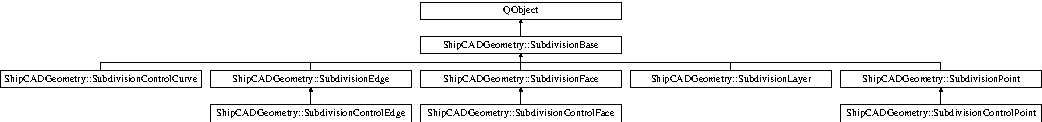
\includegraphics[height=1.641026cm]{classShipCADGeometry_1_1SubdivisionBase}
\end{center}
\end{figure}
\subsection*{Public Member Functions}
\begin{DoxyCompactItemize}
\item 
\hyperlink{classShipCADGeometry_1_1SubdivisionBase_ad424b99e73d138f565a152ed0ee648cb}{Subdivision\-Base} (\hyperlink{classShipCADGeometry_1_1SubdivisionSurface}{Subdivision\-Surface} $\ast$owner)
\begin{DoxyCompactList}\small\item\em Constructor. \end{DoxyCompactList}\item 
virtual \hyperlink{classShipCADGeometry_1_1SubdivisionBase_a12b4adebcd9fb52d4d82d9ff469e144d}{$\sim$\-Subdivision\-Base} ()
\item 
\hyperlink{classShipCADGeometry_1_1SubdivisionSurface}{Subdivision\-Surface} $\ast$ \hyperlink{classShipCADGeometry_1_1SubdivisionBase_a6003c22ab0149e6f01beff5dde397370}{get\-Owner} ()
\begin{DoxyCompactList}\small\item\em get the owning surface \end{DoxyCompactList}\item 
virtual void \hyperlink{classShipCADGeometry_1_1SubdivisionBase_a8e4716f15f6a81c2c5dd26b9931ecb91}{set\-Owner} (\hyperlink{classShipCADGeometry_1_1SubdivisionSurface}{Subdivision\-Surface} $\ast$newowner)
\begin{DoxyCompactList}\small\item\em set the owing surface \end{DoxyCompactList}\item 
virtual void \hyperlink{classShipCADGeometry_1_1SubdivisionBase_ae668920d97c0810c72996a531e0ca107}{clear} ()=0
\begin{DoxyCompactList}\small\item\em reset this element to default values \end{DoxyCompactList}\item 
virtual void \hyperlink{classShipCADGeometry_1_1SubdivisionBase_a7807e64ac8d2acc3da572e03cf0523b6}{dump} (std\-::ostream \&os, const char $\ast$prefix=\char`\"{}\char`\"{}) const 
\begin{DoxyCompactList}\small\item\em print out the element to a stream \end{DoxyCompactList}\end{DoxyCompactItemize}
\subsection*{Protected Member Functions}
\begin{DoxyCompactItemize}
\item 
void \hyperlink{classShipCADGeometry_1_1SubdivisionBase_a024aa781bbf2e54b6fb088e33126998e}{priv\-\_\-dump} (std\-::ostream \&os, const char $\ast$prefix) const 
\begin{DoxyCompactList}\small\item\em dump the element to a stream \end{DoxyCompactList}\end{DoxyCompactItemize}
\subsection*{Protected Attributes}
\begin{DoxyCompactItemize}
\item 
\hyperlink{classShipCADGeometry_1_1SubdivisionSurface}{Subdivision\-Surface} $\ast$ \hyperlink{classShipCADGeometry_1_1SubdivisionBase_a5a9ce820f644a1ecd9ddb802270f31a9}{\-\_\-owner}
\end{DoxyCompactItemize}
\subsection*{Properties}
\begin{DoxyCompactItemize}
\item 
\hyperlink{classShipCADGeometry_1_1SubdivisionSurface}{Subdivision\-Surface} \hyperlink{classShipCADGeometry_1_1SubdivisionBase_af3adf1c6df9fd4ddb5c945193fe5c65e}{Owner}
\end{DoxyCompactItemize}


\subsection{Detailed Description}
the base class for all subdivision points, edges and faces 



Definition at line 46 of file subdivbase.\-h.



\subsection{Constructor \& Destructor Documentation}
\hypertarget{classShipCADGeometry_1_1SubdivisionBase_ad424b99e73d138f565a152ed0ee648cb}{\index{Ship\-C\-A\-D\-Geometry\-::\-Subdivision\-Base@{Ship\-C\-A\-D\-Geometry\-::\-Subdivision\-Base}!Subdivision\-Base@{Subdivision\-Base}}
\index{Subdivision\-Base@{Subdivision\-Base}!ShipCADGeometry::SubdivisionBase@{Ship\-C\-A\-D\-Geometry\-::\-Subdivision\-Base}}
\subsubsection[{Subdivision\-Base}]{\setlength{\rightskip}{0pt plus 5cm}Subdivision\-Base\-::\-Subdivision\-Base (
\begin{DoxyParamCaption}
\item[{{\bf Subdivision\-Surface} $\ast$}]{owner}
\end{DoxyParamCaption}
)\hspace{0.3cm}{\ttfamily [explicit]}}}\label{classShipCADGeometry_1_1SubdivisionBase_ad424b99e73d138f565a152ed0ee648cb}


Constructor. 


\begin{DoxyParams}{Parameters}
{\em owner} & which surface this element belongs to \\
\hline
\end{DoxyParams}


Definition at line 40 of file subdivbase.\-cpp.

\hypertarget{classShipCADGeometry_1_1SubdivisionBase_a12b4adebcd9fb52d4d82d9ff469e144d}{\index{Ship\-C\-A\-D\-Geometry\-::\-Subdivision\-Base@{Ship\-C\-A\-D\-Geometry\-::\-Subdivision\-Base}!$\sim$\-Subdivision\-Base@{$\sim$\-Subdivision\-Base}}
\index{$\sim$\-Subdivision\-Base@{$\sim$\-Subdivision\-Base}!ShipCADGeometry::SubdivisionBase@{Ship\-C\-A\-D\-Geometry\-::\-Subdivision\-Base}}
\subsubsection[{$\sim$\-Subdivision\-Base}]{\setlength{\rightskip}{0pt plus 5cm}Subdivision\-Base\-::$\sim$\-Subdivision\-Base (
\begin{DoxyParamCaption}
{}
\end{DoxyParamCaption}
)\hspace{0.3cm}{\ttfamily [virtual]}}}\label{classShipCADGeometry_1_1SubdivisionBase_a12b4adebcd9fb52d4d82d9ff469e144d}


Definition at line 46 of file subdivbase.\-cpp.



\subsection{Member Function Documentation}
\hypertarget{classShipCADGeometry_1_1SubdivisionBase_ae668920d97c0810c72996a531e0ca107}{\index{Ship\-C\-A\-D\-Geometry\-::\-Subdivision\-Base@{Ship\-C\-A\-D\-Geometry\-::\-Subdivision\-Base}!clear@{clear}}
\index{clear@{clear}!ShipCADGeometry::SubdivisionBase@{Ship\-C\-A\-D\-Geometry\-::\-Subdivision\-Base}}
\subsubsection[{clear}]{\setlength{\rightskip}{0pt plus 5cm}virtual void Ship\-C\-A\-D\-Geometry\-::\-Subdivision\-Base\-::clear (
\begin{DoxyParamCaption}
{}
\end{DoxyParamCaption}
)\hspace{0.3cm}{\ttfamily [pure virtual]}}}\label{classShipCADGeometry_1_1SubdivisionBase_ae668920d97c0810c72996a531e0ca107}


reset this element to default values 



Implemented in \hyperlink{classShipCADGeometry_1_1SubdivisionControlFace_ad168e31f0ef2537b3cd0f58b0c1c54e2}{Ship\-C\-A\-D\-Geometry\-::\-Subdivision\-Control\-Face}, \hyperlink{classShipCADGeometry_1_1SubdivisionPoint_aef22d2b6cb48e57ce69652eeb7a69711}{Ship\-C\-A\-D\-Geometry\-::\-Subdivision\-Point}, \hyperlink{classShipCADGeometry_1_1SubdivisionLayer_a7046d17ba87dd5ce7399f22ae327fc6e}{Ship\-C\-A\-D\-Geometry\-::\-Subdivision\-Layer}, \hyperlink{classShipCADGeometry_1_1SubdivisionControlCurve_aa574f77f4abc5a8eef05e7cef7f8d8a2}{Ship\-C\-A\-D\-Geometry\-::\-Subdivision\-Control\-Curve}, \hyperlink{classShipCADGeometry_1_1SubdivisionFace_a413ae7e76f559780c8a69e998974fb75}{Ship\-C\-A\-D\-Geometry\-::\-Subdivision\-Face}, and \hyperlink{classShipCADGeometry_1_1SubdivisionEdge_a08358ac65c2d710855b8b93c64ce9d02}{Ship\-C\-A\-D\-Geometry\-::\-Subdivision\-Edge}.

\hypertarget{classShipCADGeometry_1_1SubdivisionBase_a7807e64ac8d2acc3da572e03cf0523b6}{\index{Ship\-C\-A\-D\-Geometry\-::\-Subdivision\-Base@{Ship\-C\-A\-D\-Geometry\-::\-Subdivision\-Base}!dump@{dump}}
\index{dump@{dump}!ShipCADGeometry::SubdivisionBase@{Ship\-C\-A\-D\-Geometry\-::\-Subdivision\-Base}}
\subsubsection[{dump}]{\setlength{\rightskip}{0pt plus 5cm}void Subdivision\-Base\-::dump (
\begin{DoxyParamCaption}
\item[{std\-::ostream \&}]{os, }
\item[{const char $\ast$}]{prefix = {\ttfamily \char`\"{}\char`\"{}}}
\end{DoxyParamCaption}
) const\hspace{0.3cm}{\ttfamily [virtual]}}}\label{classShipCADGeometry_1_1SubdivisionBase_a7807e64ac8d2acc3da572e03cf0523b6}


print out the element to a stream 


\begin{DoxyParams}{Parameters}
{\em os} & the output stream \\
\hline
{\em prefix} & string to prefix on each line output \\
\hline
\end{DoxyParams}


Reimplemented in \hyperlink{classShipCADGeometry_1_1SubdivisionControlPoint_a4a9d6e45291c27f19f0d76c9b9d19048}{Ship\-C\-A\-D\-Geometry\-::\-Subdivision\-Control\-Point}, \hyperlink{classShipCADGeometry_1_1SubdivisionControlFace_a947868fba3e9bb6c587847fb9245c9ff}{Ship\-C\-A\-D\-Geometry\-::\-Subdivision\-Control\-Face}, \hyperlink{classShipCADGeometry_1_1SubdivisionPoint_aed72cf5e8dc67e980010d195f3a376a3}{Ship\-C\-A\-D\-Geometry\-::\-Subdivision\-Point}, \hyperlink{classShipCADGeometry_1_1SubdivisionControlEdge_abdfa96ff05eff404214a92d38d7eb715}{Ship\-C\-A\-D\-Geometry\-::\-Subdivision\-Control\-Edge}, \hyperlink{classShipCADGeometry_1_1SubdivisionLayer_ab41e005f720a2bba4b2efa74bfd5943e}{Ship\-C\-A\-D\-Geometry\-::\-Subdivision\-Layer}, \hyperlink{classShipCADGeometry_1_1SubdivisionFace_aa5bd261ae5fc0a1c7fe8cc5328b8477f}{Ship\-C\-A\-D\-Geometry\-::\-Subdivision\-Face}, \hyperlink{classShipCADGeometry_1_1SubdivisionEdge_a14cc58877644ebd7b7ebffbdf8ef87f7}{Ship\-C\-A\-D\-Geometry\-::\-Subdivision\-Edge}, and \hyperlink{classShipCADGeometry_1_1SubdivisionControlCurve_a30e8d074583a386be2ab6343cb5f8502}{Ship\-C\-A\-D\-Geometry\-::\-Subdivision\-Control\-Curve}.



Definition at line 51 of file subdivbase.\-cpp.

\hypertarget{classShipCADGeometry_1_1SubdivisionBase_a6003c22ab0149e6f01beff5dde397370}{\index{Ship\-C\-A\-D\-Geometry\-::\-Subdivision\-Base@{Ship\-C\-A\-D\-Geometry\-::\-Subdivision\-Base}!get\-Owner@{get\-Owner}}
\index{get\-Owner@{get\-Owner}!ShipCADGeometry::SubdivisionBase@{Ship\-C\-A\-D\-Geometry\-::\-Subdivision\-Base}}
\subsubsection[{get\-Owner}]{\setlength{\rightskip}{0pt plus 5cm}{\bf Subdivision\-Surface}$\ast$ Ship\-C\-A\-D\-Geometry\-::\-Subdivision\-Base\-::get\-Owner (
\begin{DoxyParamCaption}
{}
\end{DoxyParamCaption}
)\hspace{0.3cm}{\ttfamily [inline]}}}\label{classShipCADGeometry_1_1SubdivisionBase_a6003c22ab0149e6f01beff5dde397370}


get the owning surface 

\begin{DoxyReturn}{Returns}
the owning surface 
\end{DoxyReturn}


Definition at line 64 of file subdivbase.\-h.

\hypertarget{classShipCADGeometry_1_1SubdivisionBase_a024aa781bbf2e54b6fb088e33126998e}{\index{Ship\-C\-A\-D\-Geometry\-::\-Subdivision\-Base@{Ship\-C\-A\-D\-Geometry\-::\-Subdivision\-Base}!priv\-\_\-dump@{priv\-\_\-dump}}
\index{priv\-\_\-dump@{priv\-\_\-dump}!ShipCADGeometry::SubdivisionBase@{Ship\-C\-A\-D\-Geometry\-::\-Subdivision\-Base}}
\subsubsection[{priv\-\_\-dump}]{\setlength{\rightskip}{0pt plus 5cm}void Subdivision\-Base\-::priv\-\_\-dump (
\begin{DoxyParamCaption}
\item[{std\-::ostream \&}]{os, }
\item[{const char $\ast$}]{prefix}
\end{DoxyParamCaption}
) const\hspace{0.3cm}{\ttfamily [protected]}}}\label{classShipCADGeometry_1_1SubdivisionBase_a024aa781bbf2e54b6fb088e33126998e}


dump the element to a stream 


\begin{DoxyParams}{Parameters}
{\em os} & the output stream \\
\hline
{\em prefix} & string to prefix on each line output \\
\hline
\end{DoxyParams}


Definition at line 57 of file subdivbase.\-cpp.

\hypertarget{classShipCADGeometry_1_1SubdivisionBase_a8e4716f15f6a81c2c5dd26b9931ecb91}{\index{Ship\-C\-A\-D\-Geometry\-::\-Subdivision\-Base@{Ship\-C\-A\-D\-Geometry\-::\-Subdivision\-Base}!set\-Owner@{set\-Owner}}
\index{set\-Owner@{set\-Owner}!ShipCADGeometry::SubdivisionBase@{Ship\-C\-A\-D\-Geometry\-::\-Subdivision\-Base}}
\subsubsection[{set\-Owner}]{\setlength{\rightskip}{0pt plus 5cm}virtual void Ship\-C\-A\-D\-Geometry\-::\-Subdivision\-Base\-::set\-Owner (
\begin{DoxyParamCaption}
\item[{{\bf Subdivision\-Surface} $\ast$}]{newowner}
\end{DoxyParamCaption}
)\hspace{0.3cm}{\ttfamily [inline]}, {\ttfamily [virtual]}}}\label{classShipCADGeometry_1_1SubdivisionBase_a8e4716f15f6a81c2c5dd26b9931ecb91}


set the owing surface 


\begin{DoxyParams}{Parameters}
{\em newowner} & the owning surface \\
\hline
\end{DoxyParams}


Definition at line 69 of file subdivbase.\-h.



\subsection{Member Data Documentation}
\hypertarget{classShipCADGeometry_1_1SubdivisionBase_a5a9ce820f644a1ecd9ddb802270f31a9}{\index{Ship\-C\-A\-D\-Geometry\-::\-Subdivision\-Base@{Ship\-C\-A\-D\-Geometry\-::\-Subdivision\-Base}!\-\_\-owner@{\-\_\-owner}}
\index{\-\_\-owner@{\-\_\-owner}!ShipCADGeometry::SubdivisionBase@{Ship\-C\-A\-D\-Geometry\-::\-Subdivision\-Base}}
\subsubsection[{\-\_\-owner}]{\setlength{\rightskip}{0pt plus 5cm}{\bf Subdivision\-Surface}$\ast$ Ship\-C\-A\-D\-Geometry\-::\-Subdivision\-Base\-::\-\_\-owner\hspace{0.3cm}{\ttfamily [protected]}}}\label{classShipCADGeometry_1_1SubdivisionBase_a5a9ce820f644a1ecd9ddb802270f31a9}
the owning surface 

Definition at line 94 of file subdivbase.\-h.



\subsection{Property Documentation}
\hypertarget{classShipCADGeometry_1_1SubdivisionBase_af3adf1c6df9fd4ddb5c945193fe5c65e}{\index{Ship\-C\-A\-D\-Geometry\-::\-Subdivision\-Base@{Ship\-C\-A\-D\-Geometry\-::\-Subdivision\-Base}!Owner@{Owner}}
\index{Owner@{Owner}!ShipCADGeometry::SubdivisionBase@{Ship\-C\-A\-D\-Geometry\-::\-Subdivision\-Base}}
\subsubsection[{Owner}]{\setlength{\rightskip}{0pt plus 5cm}{\bf Subdivision\-Surface} Ship\-C\-A\-D\-Geometry\-::\-Subdivision\-Base\-::\-Owner\hspace{0.3cm}{\ttfamily [read]}}}\label{classShipCADGeometry_1_1SubdivisionBase_af3adf1c6df9fd4ddb5c945193fe5c65e}


Definition at line 49 of file subdivbase.\-h.



The documentation for this class was generated from the following files\-:\begin{DoxyCompactItemize}
\item 
Ship\-C\-A\-Dlib/\hyperlink{subdivbase_8h}{subdivbase.\-h}\item 
Ship\-C\-A\-Dlib/\hyperlink{subdivbase_8cpp}{subdivbase.\-cpp}\end{DoxyCompactItemize}

\hypertarget{classShipCADGeometry_1_1SubdivisionControlCurve}{\section{Ship\-C\-A\-D\-Geometry\-:\-:Subdivision\-Control\-Curve Class Reference}
\label{classShipCADGeometry_1_1SubdivisionControlCurve}\index{Ship\-C\-A\-D\-Geometry\-::\-Subdivision\-Control\-Curve@{Ship\-C\-A\-D\-Geometry\-::\-Subdivision\-Control\-Curve}}
}


{\ttfamily \#include $<$subdivcontrolcurve.\-h$>$}

Inheritance diagram for Ship\-C\-A\-D\-Geometry\-:\-:Subdivision\-Control\-Curve\-:\begin{figure}[H]
\begin{center}
\leavevmode
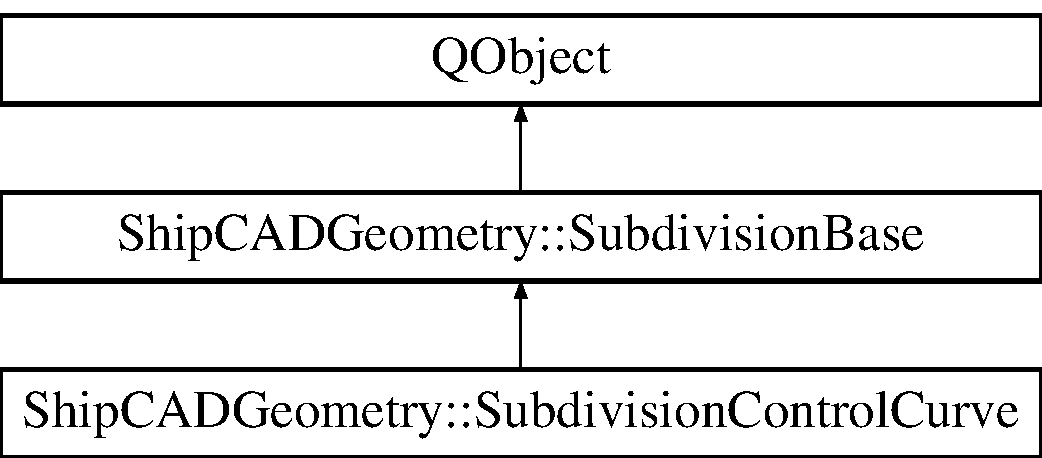
\includegraphics[height=3.000000cm]{classShipCADGeometry_1_1SubdivisionControlCurve}
\end{center}
\end{figure}
\subsection*{Public Member Functions}
\begin{DoxyCompactItemize}
\item 
\hyperlink{classShipCADGeometry_1_1SubdivisionControlCurve_adfdaa3dcd794901f3c1277223eab22f9}{Subdivision\-Control\-Curve} (\hyperlink{classShipCADGeometry_1_1SubdivisionSurface}{Subdivision\-Surface} $\ast$owner)
\item 
virtual \hyperlink{classShipCADGeometry_1_1SubdivisionControlCurve_a5b3d3e0b700afd7a7a1da0e5dfafdfb9}{$\sim$\-Subdivision\-Control\-Curve} ()
\item 
void \hyperlink{classShipCADGeometry_1_1SubdivisionControlCurve_a078fc8820a6c0e37c475eec1897b13dd}{replace\-Vertex\-Point} (\hyperlink{classShipCADGeometry_1_1SubdivisionPoint}{Subdivision\-Point} $\ast$oldpt, \hyperlink{classShipCADGeometry_1_1SubdivisionPoint}{Subdivision\-Point} $\ast$newpt)
\item 
void \hyperlink{classShipCADGeometry_1_1SubdivisionControlCurve_a0764f5d7697b76ac928a121d224733f5}{insert\-Edge\-Point} (\hyperlink{classShipCADGeometry_1_1SubdivisionPoint}{Subdivision\-Point} $\ast$p1, \hyperlink{classShipCADGeometry_1_1SubdivisionPoint}{Subdivision\-Point} $\ast$p2, \hyperlink{classShipCADGeometry_1_1SubdivisionPoint}{Subdivision\-Point} $\ast$newpt)
\item 
void \hyperlink{classShipCADGeometry_1_1SubdivisionControlCurve_abfed48331919c4d2a2bfc6363b28ebb4}{delete\-Edge} (\hyperlink{classShipCADGeometry_1_1SubdivisionControlEdge}{Subdivision\-Control\-Edge} $\ast$edge)
\item 
void \hyperlink{classShipCADGeometry_1_1SubdivisionControlCurve_a9469b178a88269d0f9ee3b17d5f15272}{insert\-Control\-Point} (\hyperlink{classShipCADGeometry_1_1SubdivisionControlPoint}{Subdivision\-Control\-Point} $\ast$p1, \hyperlink{classShipCADGeometry_1_1SubdivisionControlPoint}{Subdivision\-Control\-Point} $\ast$p2, \hyperlink{classShipCADGeometry_1_1SubdivisionControlPoint}{Subdivision\-Control\-Point} $\ast$newpt)
\item 
void \hyperlink{classShipCADGeometry_1_1SubdivisionControlCurve_a1155b0abe401a7128369a589b6e6ac9c}{add\-Point} (\hyperlink{classShipCADGeometry_1_1SubdivisionControlPoint}{Subdivision\-Control\-Point} $\ast$p)
\item 
virtual void \hyperlink{classShipCADGeometry_1_1SubdivisionControlCurve_aa574f77f4abc5a8eef05e7cef7f8d8a2}{clear} ()
\item 
void \hyperlink{classShipCADGeometry_1_1SubdivisionControlCurve_a34e280e9ba6e6705577d1afd229e9f20}{reset\-Div\-Points} ()
\item 
bool \hyperlink{classShipCADGeometry_1_1SubdivisionControlCurve_a8b3c57aba1c16b77b902daacd7b88d0c}{is\-Selected} ()
\item 
bool \hyperlink{classShipCADGeometry_1_1SubdivisionControlCurve_a36bcf74cf20d7f1ae888f25f774b040d}{is\-Visible} ()
\item 
bool \hyperlink{classShipCADGeometry_1_1SubdivisionControlCurve_a16750d28e492cadbb3dd0f1ad303512e}{is\-Build} ()
\item 
Q\-Color \hyperlink{classShipCADGeometry_1_1SubdivisionControlCurve_a1dd7d33fd574c3cfdd53ccbb13abb695}{get\-Color} ()
\item 
size\-\_\-t \hyperlink{classShipCADGeometry_1_1SubdivisionControlCurve_a28c99c59aa80008a27cec27e8aada56b}{number\-Of\-Control\-Points} ()
\item 
size\-\_\-t \hyperlink{classShipCADGeometry_1_1SubdivisionControlCurve_a98ca6b2a39a99d0cee63263df65c6c1e}{number\-Of\-Subdiv\-Points} ()
\item 
\hyperlink{classShipCADGeometry_1_1SubdivisionControlPoint}{Subdivision\-Control\-Point} $\ast$ \hyperlink{classShipCADGeometry_1_1SubdivisionControlCurve_a0331fade870dd4856c070e2f487882b5}{get\-Control\-Point} (size\-\_\-t index)
\item 
\hyperlink{classShipCADGeometry_1_1SubdivisionPoint}{Subdivision\-Point} $\ast$ \hyperlink{classShipCADGeometry_1_1SubdivisionControlCurve_a52b12b58d524baba317ab6504e80018f}{get\-Subdiv\-Point} (size\-\_\-t index)
\item 
void \hyperlink{classShipCADGeometry_1_1SubdivisionControlCurve_a585a51955a6e91642b01d474eeef0d4f}{set\-Visible} (bool val)
\item 
void \hyperlink{classShipCADGeometry_1_1SubdivisionControlCurve_a698e6153097398da8fe2c6ecf2f2408b}{set\-Build} (bool val)
\item 
void \hyperlink{classShipCADGeometry_1_1SubdivisionControlCurve_abaf7f7cfec21eedacf55b1654f3e7f2f}{set\-Selected} (bool val)
\item 
\hyperlink{classShipCADGeometry_1_1Spline}{Spline} $\ast$ \hyperlink{classShipCADGeometry_1_1SubdivisionControlCurve_a6c62247f84c62bded5c291c54623f0f6}{get\-Spline} ()
\item 
void \hyperlink{classShipCADGeometry_1_1SubdivisionControlCurve_ad2a7118ea074ce1b7f61586f08039d2a}{load\-Binary} (\hyperlink{classShipCADGeometry_1_1FileBuffer}{File\-Buffer} \&source)
\item 
void \hyperlink{classShipCADGeometry_1_1SubdivisionControlCurve_a3ef4c7ce3e2d9a2fe4f90ebf35ffc033}{save\-Binary} (\hyperlink{classShipCADGeometry_1_1FileBuffer}{File\-Buffer} \&destiniation)
\item 
void \hyperlink{classShipCADGeometry_1_1SubdivisionControlCurve_a22726dc4edf385c5b4b5fead84d4c3de}{save\-To\-D\-X\-F} (std\-::vector$<$ Q\-String $>$ \&strings)
\item 
virtual void \hyperlink{classShipCADGeometry_1_1SubdivisionControlCurve_a4d7d8e87dc582529e763039ffe593360}{draw} (\hyperlink{classShipCADGeometry_1_1Viewport}{Viewport} \&vp, \hyperlink{classShipCADGeometry_1_1LineShader}{Line\-Shader} $\ast$lineshader)
\item 
virtual void \hyperlink{classShipCADGeometry_1_1SubdivisionControlCurve_a30e8d074583a386be2ab6343cb5f8502}{dump} (std\-::ostream \&os, const char $\ast$prefix=\char`\"{}\char`\"{}) const 
\end{DoxyCompactItemize}
\subsection*{Static Public Member Functions}
\begin{DoxyCompactItemize}
\item 
static \hyperlink{classShipCADGeometry_1_1SubdivisionControlCurve}{Subdivision\-Control\-Curve} $\ast$ \hyperlink{classShipCADGeometry_1_1SubdivisionControlCurve_a21d9226cc2fd7efcaf6f1067912a0b34}{construct} (\hyperlink{classShipCADGeometry_1_1SubdivisionSurface}{Subdivision\-Surface} $\ast$owner)
\end{DoxyCompactItemize}
\subsection*{Protected Member Functions}
\begin{DoxyCompactItemize}
\item 
void \hyperlink{classShipCADGeometry_1_1SubdivisionControlCurve_a48fbb761e8c85120ba7f6876d873e898}{priv\-\_\-dump} (std\-::ostream \&os, const char $\ast$prefix) const 
\end{DoxyCompactItemize}
\subsection*{Protected Attributes}
\begin{DoxyCompactItemize}
\item 
bool \hyperlink{classShipCADGeometry_1_1SubdivisionControlCurve_a6467811e9b5545af5bb092199fcfde95}{\-\_\-build}
\item 
std\-::vector\\*
$<$ \hyperlink{classShipCADGeometry_1_1SubdivisionControlPoint}{Subdivision\-Control\-Point} $\ast$ $>$ \hyperlink{classShipCADGeometry_1_1SubdivisionControlCurve_aee920e208e7da3314721be340b95d504}{\-\_\-points}
\item 
std\-::vector$<$ \hyperlink{classShipCADGeometry_1_1SubdivisionPoint}{Subdivision\-Point} $\ast$ $>$ \hyperlink{classShipCADGeometry_1_1SubdivisionControlCurve_ae8df6891a3f435811616a162ec3b9a4d}{\-\_\-div\-\_\-points}
\item 
\hyperlink{classShipCADGeometry_1_1Spline}{Spline} $\ast$ \hyperlink{classShipCADGeometry_1_1SubdivisionControlCurve_a7dd9c824ab09ab75fa472bc0ffc83cb6}{\-\_\-curve}
\end{DoxyCompactItemize}
\subsection*{Additional Inherited Members}


\subsection{Detailed Description}


Definition at line 55 of file subdivcontrolcurve.\-h.



\subsection{Constructor \& Destructor Documentation}
\hypertarget{classShipCADGeometry_1_1SubdivisionControlCurve_adfdaa3dcd794901f3c1277223eab22f9}{\index{Ship\-C\-A\-D\-Geometry\-::\-Subdivision\-Control\-Curve@{Ship\-C\-A\-D\-Geometry\-::\-Subdivision\-Control\-Curve}!Subdivision\-Control\-Curve@{Subdivision\-Control\-Curve}}
\index{Subdivision\-Control\-Curve@{Subdivision\-Control\-Curve}!ShipCADGeometry::SubdivisionControlCurve@{Ship\-C\-A\-D\-Geometry\-::\-Subdivision\-Control\-Curve}}
\subsubsection[{Subdivision\-Control\-Curve}]{\setlength{\rightskip}{0pt plus 5cm}Subdivision\-Control\-Curve\-::\-Subdivision\-Control\-Curve (
\begin{DoxyParamCaption}
\item[{{\bf Subdivision\-Surface} $\ast$}]{owner}
\end{DoxyParamCaption}
)\hspace{0.3cm}{\ttfamily [explicit]}}}\label{classShipCADGeometry_1_1SubdivisionControlCurve_adfdaa3dcd794901f3c1277223eab22f9}


Definition at line 56 of file subdivcontrolcurve.\-cpp.

\hypertarget{classShipCADGeometry_1_1SubdivisionControlCurve_a5b3d3e0b700afd7a7a1da0e5dfafdfb9}{\index{Ship\-C\-A\-D\-Geometry\-::\-Subdivision\-Control\-Curve@{Ship\-C\-A\-D\-Geometry\-::\-Subdivision\-Control\-Curve}!$\sim$\-Subdivision\-Control\-Curve@{$\sim$\-Subdivision\-Control\-Curve}}
\index{$\sim$\-Subdivision\-Control\-Curve@{$\sim$\-Subdivision\-Control\-Curve}!ShipCADGeometry::SubdivisionControlCurve@{Ship\-C\-A\-D\-Geometry\-::\-Subdivision\-Control\-Curve}}
\subsubsection[{$\sim$\-Subdivision\-Control\-Curve}]{\setlength{\rightskip}{0pt plus 5cm}Subdivision\-Control\-Curve\-::$\sim$\-Subdivision\-Control\-Curve (
\begin{DoxyParamCaption}
{}
\end{DoxyParamCaption}
)\hspace{0.3cm}{\ttfamily [virtual]}}}\label{classShipCADGeometry_1_1SubdivisionControlCurve_a5b3d3e0b700afd7a7a1da0e5dfafdfb9}


Definition at line 62 of file subdivcontrolcurve.\-cpp.



\subsection{Member Function Documentation}
\hypertarget{classShipCADGeometry_1_1SubdivisionControlCurve_a1155b0abe401a7128369a589b6e6ac9c}{\index{Ship\-C\-A\-D\-Geometry\-::\-Subdivision\-Control\-Curve@{Ship\-C\-A\-D\-Geometry\-::\-Subdivision\-Control\-Curve}!add\-Point@{add\-Point}}
\index{add\-Point@{add\-Point}!ShipCADGeometry::SubdivisionControlCurve@{Ship\-C\-A\-D\-Geometry\-::\-Subdivision\-Control\-Curve}}
\subsubsection[{add\-Point}]{\setlength{\rightskip}{0pt plus 5cm}void Subdivision\-Control\-Curve\-::add\-Point (
\begin{DoxyParamCaption}
\item[{{\bf Subdivision\-Control\-Point} $\ast$}]{p}
\end{DoxyParamCaption}
)}}\label{classShipCADGeometry_1_1SubdivisionControlCurve_a1155b0abe401a7128369a589b6e6ac9c}


Definition at line 95 of file subdivcontrolcurve.\-cpp.

\hypertarget{classShipCADGeometry_1_1SubdivisionControlCurve_aa574f77f4abc5a8eef05e7cef7f8d8a2}{\index{Ship\-C\-A\-D\-Geometry\-::\-Subdivision\-Control\-Curve@{Ship\-C\-A\-D\-Geometry\-::\-Subdivision\-Control\-Curve}!clear@{clear}}
\index{clear@{clear}!ShipCADGeometry::SubdivisionControlCurve@{Ship\-C\-A\-D\-Geometry\-::\-Subdivision\-Control\-Curve}}
\subsubsection[{clear}]{\setlength{\rightskip}{0pt plus 5cm}void Subdivision\-Control\-Curve\-::clear (
\begin{DoxyParamCaption}
{}
\end{DoxyParamCaption}
)\hspace{0.3cm}{\ttfamily [virtual]}}}\label{classShipCADGeometry_1_1SubdivisionControlCurve_aa574f77f4abc5a8eef05e7cef7f8d8a2}


Implements \hyperlink{classShipCADGeometry_1_1SubdivisionBase_ae668920d97c0810c72996a531e0ca107}{Ship\-C\-A\-D\-Geometry\-::\-Subdivision\-Base}.



Definition at line 140 of file subdivcontrolcurve.\-cpp.

\hypertarget{classShipCADGeometry_1_1SubdivisionControlCurve_a21d9226cc2fd7efcaf6f1067912a0b34}{\index{Ship\-C\-A\-D\-Geometry\-::\-Subdivision\-Control\-Curve@{Ship\-C\-A\-D\-Geometry\-::\-Subdivision\-Control\-Curve}!construct@{construct}}
\index{construct@{construct}!ShipCADGeometry::SubdivisionControlCurve@{Ship\-C\-A\-D\-Geometry\-::\-Subdivision\-Control\-Curve}}
\subsubsection[{construct}]{\setlength{\rightskip}{0pt plus 5cm}{\bf Subdivision\-Control\-Curve} $\ast$ Subdivision\-Control\-Curve\-::construct (
\begin{DoxyParamCaption}
\item[{{\bf Subdivision\-Surface} $\ast$}]{owner}
\end{DoxyParamCaption}
)\hspace{0.3cm}{\ttfamily [static]}}}\label{classShipCADGeometry_1_1SubdivisionControlCurve_a21d9226cc2fd7efcaf6f1067912a0b34}


Definition at line 48 of file subdivcontrolcurve.\-cpp.

\hypertarget{classShipCADGeometry_1_1SubdivisionControlCurve_abfed48331919c4d2a2bfc6363b28ebb4}{\index{Ship\-C\-A\-D\-Geometry\-::\-Subdivision\-Control\-Curve@{Ship\-C\-A\-D\-Geometry\-::\-Subdivision\-Control\-Curve}!delete\-Edge@{delete\-Edge}}
\index{delete\-Edge@{delete\-Edge}!ShipCADGeometry::SubdivisionControlCurve@{Ship\-C\-A\-D\-Geometry\-::\-Subdivision\-Control\-Curve}}
\subsubsection[{delete\-Edge}]{\setlength{\rightskip}{0pt plus 5cm}void Subdivision\-Control\-Curve\-::delete\-Edge (
\begin{DoxyParamCaption}
\item[{{\bf Subdivision\-Control\-Edge} $\ast$}]{edge}
\end{DoxyParamCaption}
)}}\label{classShipCADGeometry_1_1SubdivisionControlCurve_abfed48331919c4d2a2bfc6363b28ebb4}


Definition at line 148 of file subdivcontrolcurve.\-cpp.

\hypertarget{classShipCADGeometry_1_1SubdivisionControlCurve_a4d7d8e87dc582529e763039ffe593360}{\index{Ship\-C\-A\-D\-Geometry\-::\-Subdivision\-Control\-Curve@{Ship\-C\-A\-D\-Geometry\-::\-Subdivision\-Control\-Curve}!draw@{draw}}
\index{draw@{draw}!ShipCADGeometry::SubdivisionControlCurve@{Ship\-C\-A\-D\-Geometry\-::\-Subdivision\-Control\-Curve}}
\subsubsection[{draw}]{\setlength{\rightskip}{0pt plus 5cm}void Subdivision\-Control\-Curve\-::draw (
\begin{DoxyParamCaption}
\item[{{\bf Viewport} \&}]{vp, }
\item[{{\bf Line\-Shader} $\ast$}]{lineshader}
\end{DoxyParamCaption}
)\hspace{0.3cm}{\ttfamily [virtual]}}}\label{classShipCADGeometry_1_1SubdivisionControlCurve_a4d7d8e87dc582529e763039ffe593360}


Definition at line 221 of file subdivcontrolcurve.\-cpp.

\hypertarget{classShipCADGeometry_1_1SubdivisionControlCurve_a30e8d074583a386be2ab6343cb5f8502}{\index{Ship\-C\-A\-D\-Geometry\-::\-Subdivision\-Control\-Curve@{Ship\-C\-A\-D\-Geometry\-::\-Subdivision\-Control\-Curve}!dump@{dump}}
\index{dump@{dump}!ShipCADGeometry::SubdivisionControlCurve@{Ship\-C\-A\-D\-Geometry\-::\-Subdivision\-Control\-Curve}}
\subsubsection[{dump}]{\setlength{\rightskip}{0pt plus 5cm}void Subdivision\-Control\-Curve\-::dump (
\begin{DoxyParamCaption}
\item[{std\-::ostream \&}]{os, }
\item[{const char $\ast$}]{prefix = {\ttfamily \char`\"{}\char`\"{}}}
\end{DoxyParamCaption}
) const\hspace{0.3cm}{\ttfamily [virtual]}}}\label{classShipCADGeometry_1_1SubdivisionControlCurve_a30e8d074583a386be2ab6343cb5f8502}


Reimplemented from \hyperlink{classShipCADGeometry_1_1SubdivisionBase_a7807e64ac8d2acc3da572e03cf0523b6}{Ship\-C\-A\-D\-Geometry\-::\-Subdivision\-Base}.



Definition at line 401 of file subdivcontrolcurve.\-cpp.

\hypertarget{classShipCADGeometry_1_1SubdivisionControlCurve_a1dd7d33fd574c3cfdd53ccbb13abb695}{\index{Ship\-C\-A\-D\-Geometry\-::\-Subdivision\-Control\-Curve@{Ship\-C\-A\-D\-Geometry\-::\-Subdivision\-Control\-Curve}!get\-Color@{get\-Color}}
\index{get\-Color@{get\-Color}!ShipCADGeometry::SubdivisionControlCurve@{Ship\-C\-A\-D\-Geometry\-::\-Subdivision\-Control\-Curve}}
\subsubsection[{get\-Color}]{\setlength{\rightskip}{0pt plus 5cm}Q\-Color Subdivision\-Control\-Curve\-::get\-Color (
\begin{DoxyParamCaption}
{}
\end{DoxyParamCaption}
)}}\label{classShipCADGeometry_1_1SubdivisionControlCurve_a1dd7d33fd574c3cfdd53ccbb13abb695}


Definition at line 109 of file subdivcontrolcurve.\-cpp.

\hypertarget{classShipCADGeometry_1_1SubdivisionControlCurve_a0331fade870dd4856c070e2f487882b5}{\index{Ship\-C\-A\-D\-Geometry\-::\-Subdivision\-Control\-Curve@{Ship\-C\-A\-D\-Geometry\-::\-Subdivision\-Control\-Curve}!get\-Control\-Point@{get\-Control\-Point}}
\index{get\-Control\-Point@{get\-Control\-Point}!ShipCADGeometry::SubdivisionControlCurve@{Ship\-C\-A\-D\-Geometry\-::\-Subdivision\-Control\-Curve}}
\subsubsection[{get\-Control\-Point}]{\setlength{\rightskip}{0pt plus 5cm}{\bf Subdivision\-Control\-Point} $\ast$ Subdivision\-Control\-Curve\-::get\-Control\-Point (
\begin{DoxyParamCaption}
\item[{size\-\_\-t}]{index}
\end{DoxyParamCaption}
)}}\label{classShipCADGeometry_1_1SubdivisionControlCurve_a0331fade870dd4856c070e2f487882b5}


Definition at line 126 of file subdivcontrolcurve.\-cpp.

\hypertarget{classShipCADGeometry_1_1SubdivisionControlCurve_a6c62247f84c62bded5c291c54623f0f6}{\index{Ship\-C\-A\-D\-Geometry\-::\-Subdivision\-Control\-Curve@{Ship\-C\-A\-D\-Geometry\-::\-Subdivision\-Control\-Curve}!get\-Spline@{get\-Spline}}
\index{get\-Spline@{get\-Spline}!ShipCADGeometry::SubdivisionControlCurve@{Ship\-C\-A\-D\-Geometry\-::\-Subdivision\-Control\-Curve}}
\subsubsection[{get\-Spline}]{\setlength{\rightskip}{0pt plus 5cm}{\bf Spline}$\ast$ Ship\-C\-A\-D\-Geometry\-::\-Subdivision\-Control\-Curve\-::get\-Spline (
\begin{DoxyParamCaption}
{}
\end{DoxyParamCaption}
)\hspace{0.3cm}{\ttfamily [inline]}}}\label{classShipCADGeometry_1_1SubdivisionControlCurve_a6c62247f84c62bded5c291c54623f0f6}


Definition at line 87 of file subdivcontrolcurve.\-h.

\hypertarget{classShipCADGeometry_1_1SubdivisionControlCurve_a52b12b58d524baba317ab6504e80018f}{\index{Ship\-C\-A\-D\-Geometry\-::\-Subdivision\-Control\-Curve@{Ship\-C\-A\-D\-Geometry\-::\-Subdivision\-Control\-Curve}!get\-Subdiv\-Point@{get\-Subdiv\-Point}}
\index{get\-Subdiv\-Point@{get\-Subdiv\-Point}!ShipCADGeometry::SubdivisionControlCurve@{Ship\-C\-A\-D\-Geometry\-::\-Subdivision\-Control\-Curve}}
\subsubsection[{get\-Subdiv\-Point}]{\setlength{\rightskip}{0pt plus 5cm}{\bf Subdivision\-Point} $\ast$ Subdivision\-Control\-Curve\-::get\-Subdiv\-Point (
\begin{DoxyParamCaption}
\item[{size\-\_\-t}]{index}
\end{DoxyParamCaption}
)}}\label{classShipCADGeometry_1_1SubdivisionControlCurve_a52b12b58d524baba317ab6504e80018f}


Definition at line 133 of file subdivcontrolcurve.\-cpp.

\hypertarget{classShipCADGeometry_1_1SubdivisionControlCurve_a9469b178a88269d0f9ee3b17d5f15272}{\index{Ship\-C\-A\-D\-Geometry\-::\-Subdivision\-Control\-Curve@{Ship\-C\-A\-D\-Geometry\-::\-Subdivision\-Control\-Curve}!insert\-Control\-Point@{insert\-Control\-Point}}
\index{insert\-Control\-Point@{insert\-Control\-Point}!ShipCADGeometry::SubdivisionControlCurve@{Ship\-C\-A\-D\-Geometry\-::\-Subdivision\-Control\-Curve}}
\subsubsection[{insert\-Control\-Point}]{\setlength{\rightskip}{0pt plus 5cm}void Subdivision\-Control\-Curve\-::insert\-Control\-Point (
\begin{DoxyParamCaption}
\item[{{\bf Subdivision\-Control\-Point} $\ast$}]{p1, }
\item[{{\bf Subdivision\-Control\-Point} $\ast$}]{p2, }
\item[{{\bf Subdivision\-Control\-Point} $\ast$}]{newpt}
\end{DoxyParamCaption}
)}}\label{classShipCADGeometry_1_1SubdivisionControlCurve_a9469b178a88269d0f9ee3b17d5f15272}


Definition at line 325 of file subdivcontrolcurve.\-cpp.

\hypertarget{classShipCADGeometry_1_1SubdivisionControlCurve_a0764f5d7697b76ac928a121d224733f5}{\index{Ship\-C\-A\-D\-Geometry\-::\-Subdivision\-Control\-Curve@{Ship\-C\-A\-D\-Geometry\-::\-Subdivision\-Control\-Curve}!insert\-Edge\-Point@{insert\-Edge\-Point}}
\index{insert\-Edge\-Point@{insert\-Edge\-Point}!ShipCADGeometry::SubdivisionControlCurve@{Ship\-C\-A\-D\-Geometry\-::\-Subdivision\-Control\-Curve}}
\subsubsection[{insert\-Edge\-Point}]{\setlength{\rightskip}{0pt plus 5cm}void Subdivision\-Control\-Curve\-::insert\-Edge\-Point (
\begin{DoxyParamCaption}
\item[{{\bf Subdivision\-Point} $\ast$}]{p1, }
\item[{{\bf Subdivision\-Point} $\ast$}]{p2, }
\item[{{\bf Subdivision\-Point} $\ast$}]{newpt}
\end{DoxyParamCaption}
)}}\label{classShipCADGeometry_1_1SubdivisionControlCurve_a0764f5d7697b76ac928a121d224733f5}


Definition at line 337 of file subdivcontrolcurve.\-cpp.

\hypertarget{classShipCADGeometry_1_1SubdivisionControlCurve_a16750d28e492cadbb3dd0f1ad303512e}{\index{Ship\-C\-A\-D\-Geometry\-::\-Subdivision\-Control\-Curve@{Ship\-C\-A\-D\-Geometry\-::\-Subdivision\-Control\-Curve}!is\-Build@{is\-Build}}
\index{is\-Build@{is\-Build}!ShipCADGeometry::SubdivisionControlCurve@{Ship\-C\-A\-D\-Geometry\-::\-Subdivision\-Control\-Curve}}
\subsubsection[{is\-Build}]{\setlength{\rightskip}{0pt plus 5cm}bool Ship\-C\-A\-D\-Geometry\-::\-Subdivision\-Control\-Curve\-::is\-Build (
\begin{DoxyParamCaption}
{}
\end{DoxyParamCaption}
)\hspace{0.3cm}{\ttfamily [inline]}}}\label{classShipCADGeometry_1_1SubdivisionControlCurve_a16750d28e492cadbb3dd0f1ad303512e}


Definition at line 78 of file subdivcontrolcurve.\-h.

\hypertarget{classShipCADGeometry_1_1SubdivisionControlCurve_a8b3c57aba1c16b77b902daacd7b88d0c}{\index{Ship\-C\-A\-D\-Geometry\-::\-Subdivision\-Control\-Curve@{Ship\-C\-A\-D\-Geometry\-::\-Subdivision\-Control\-Curve}!is\-Selected@{is\-Selected}}
\index{is\-Selected@{is\-Selected}!ShipCADGeometry::SubdivisionControlCurve@{Ship\-C\-A\-D\-Geometry\-::\-Subdivision\-Control\-Curve}}
\subsubsection[{is\-Selected}]{\setlength{\rightskip}{0pt plus 5cm}bool Subdivision\-Control\-Curve\-::is\-Selected (
\begin{DoxyParamCaption}
{}
\end{DoxyParamCaption}
)}}\label{classShipCADGeometry_1_1SubdivisionControlCurve_a8b3c57aba1c16b77b902daacd7b88d0c}


Definition at line 116 of file subdivcontrolcurve.\-cpp.

\hypertarget{classShipCADGeometry_1_1SubdivisionControlCurve_a36bcf74cf20d7f1ae888f25f774b040d}{\index{Ship\-C\-A\-D\-Geometry\-::\-Subdivision\-Control\-Curve@{Ship\-C\-A\-D\-Geometry\-::\-Subdivision\-Control\-Curve}!is\-Visible@{is\-Visible}}
\index{is\-Visible@{is\-Visible}!ShipCADGeometry::SubdivisionControlCurve@{Ship\-C\-A\-D\-Geometry\-::\-Subdivision\-Control\-Curve}}
\subsubsection[{is\-Visible}]{\setlength{\rightskip}{0pt plus 5cm}bool Subdivision\-Control\-Curve\-::is\-Visible (
\begin{DoxyParamCaption}
{}
\end{DoxyParamCaption}
)}}\label{classShipCADGeometry_1_1SubdivisionControlCurve_a36bcf74cf20d7f1ae888f25f774b040d}


Definition at line 121 of file subdivcontrolcurve.\-cpp.

\hypertarget{classShipCADGeometry_1_1SubdivisionControlCurve_ad2a7118ea074ce1b7f61586f08039d2a}{\index{Ship\-C\-A\-D\-Geometry\-::\-Subdivision\-Control\-Curve@{Ship\-C\-A\-D\-Geometry\-::\-Subdivision\-Control\-Curve}!load\-Binary@{load\-Binary}}
\index{load\-Binary@{load\-Binary}!ShipCADGeometry::SubdivisionControlCurve@{Ship\-C\-A\-D\-Geometry\-::\-Subdivision\-Control\-Curve}}
\subsubsection[{load\-Binary}]{\setlength{\rightskip}{0pt plus 5cm}void Subdivision\-Control\-Curve\-::load\-Binary (
\begin{DoxyParamCaption}
\item[{{\bf File\-Buffer} \&}]{source}
\end{DoxyParamCaption}
)}}\label{classShipCADGeometry_1_1SubdivisionControlCurve_ad2a7118ea074ce1b7f61586f08039d2a}


Definition at line 349 of file subdivcontrolcurve.\-cpp.

\hypertarget{classShipCADGeometry_1_1SubdivisionControlCurve_a28c99c59aa80008a27cec27e8aada56b}{\index{Ship\-C\-A\-D\-Geometry\-::\-Subdivision\-Control\-Curve@{Ship\-C\-A\-D\-Geometry\-::\-Subdivision\-Control\-Curve}!number\-Of\-Control\-Points@{number\-Of\-Control\-Points}}
\index{number\-Of\-Control\-Points@{number\-Of\-Control\-Points}!ShipCADGeometry::SubdivisionControlCurve@{Ship\-C\-A\-D\-Geometry\-::\-Subdivision\-Control\-Curve}}
\subsubsection[{number\-Of\-Control\-Points}]{\setlength{\rightskip}{0pt plus 5cm}size\-\_\-t Ship\-C\-A\-D\-Geometry\-::\-Subdivision\-Control\-Curve\-::number\-Of\-Control\-Points (
\begin{DoxyParamCaption}
{}
\end{DoxyParamCaption}
)\hspace{0.3cm}{\ttfamily [inline]}}}\label{classShipCADGeometry_1_1SubdivisionControlCurve_a28c99c59aa80008a27cec27e8aada56b}


Definition at line 80 of file subdivcontrolcurve.\-h.

\hypertarget{classShipCADGeometry_1_1SubdivisionControlCurve_a98ca6b2a39a99d0cee63263df65c6c1e}{\index{Ship\-C\-A\-D\-Geometry\-::\-Subdivision\-Control\-Curve@{Ship\-C\-A\-D\-Geometry\-::\-Subdivision\-Control\-Curve}!number\-Of\-Subdiv\-Points@{number\-Of\-Subdiv\-Points}}
\index{number\-Of\-Subdiv\-Points@{number\-Of\-Subdiv\-Points}!ShipCADGeometry::SubdivisionControlCurve@{Ship\-C\-A\-D\-Geometry\-::\-Subdivision\-Control\-Curve}}
\subsubsection[{number\-Of\-Subdiv\-Points}]{\setlength{\rightskip}{0pt plus 5cm}size\-\_\-t Ship\-C\-A\-D\-Geometry\-::\-Subdivision\-Control\-Curve\-::number\-Of\-Subdiv\-Points (
\begin{DoxyParamCaption}
{}
\end{DoxyParamCaption}
)\hspace{0.3cm}{\ttfamily [inline]}}}\label{classShipCADGeometry_1_1SubdivisionControlCurve_a98ca6b2a39a99d0cee63263df65c6c1e}


Definition at line 81 of file subdivcontrolcurve.\-h.

\hypertarget{classShipCADGeometry_1_1SubdivisionControlCurve_a48fbb761e8c85120ba7f6876d873e898}{\index{Ship\-C\-A\-D\-Geometry\-::\-Subdivision\-Control\-Curve@{Ship\-C\-A\-D\-Geometry\-::\-Subdivision\-Control\-Curve}!priv\-\_\-dump@{priv\-\_\-dump}}
\index{priv\-\_\-dump@{priv\-\_\-dump}!ShipCADGeometry::SubdivisionControlCurve@{Ship\-C\-A\-D\-Geometry\-::\-Subdivision\-Control\-Curve}}
\subsubsection[{priv\-\_\-dump}]{\setlength{\rightskip}{0pt plus 5cm}void Subdivision\-Control\-Curve\-::priv\-\_\-dump (
\begin{DoxyParamCaption}
\item[{std\-::ostream \&}]{os, }
\item[{const char $\ast$}]{prefix}
\end{DoxyParamCaption}
) const\hspace{0.3cm}{\ttfamily [protected]}}}\label{classShipCADGeometry_1_1SubdivisionControlCurve_a48fbb761e8c85120ba7f6876d873e898}


Definition at line 408 of file subdivcontrolcurve.\-cpp.

\hypertarget{classShipCADGeometry_1_1SubdivisionControlCurve_a078fc8820a6c0e37c475eec1897b13dd}{\index{Ship\-C\-A\-D\-Geometry\-::\-Subdivision\-Control\-Curve@{Ship\-C\-A\-D\-Geometry\-::\-Subdivision\-Control\-Curve}!replace\-Vertex\-Point@{replace\-Vertex\-Point}}
\index{replace\-Vertex\-Point@{replace\-Vertex\-Point}!ShipCADGeometry::SubdivisionControlCurve@{Ship\-C\-A\-D\-Geometry\-::\-Subdivision\-Control\-Curve}}
\subsubsection[{replace\-Vertex\-Point}]{\setlength{\rightskip}{0pt plus 5cm}void Subdivision\-Control\-Curve\-::replace\-Vertex\-Point (
\begin{DoxyParamCaption}
\item[{{\bf Subdivision\-Point} $\ast$}]{oldpt, }
\item[{{\bf Subdivision\-Point} $\ast$}]{newpt}
\end{DoxyParamCaption}
)}}\label{classShipCADGeometry_1_1SubdivisionControlCurve_a078fc8820a6c0e37c475eec1897b13dd}


Definition at line 373 of file subdivcontrolcurve.\-cpp.

\hypertarget{classShipCADGeometry_1_1SubdivisionControlCurve_a34e280e9ba6e6705577d1afd229e9f20}{\index{Ship\-C\-A\-D\-Geometry\-::\-Subdivision\-Control\-Curve@{Ship\-C\-A\-D\-Geometry\-::\-Subdivision\-Control\-Curve}!reset\-Div\-Points@{reset\-Div\-Points}}
\index{reset\-Div\-Points@{reset\-Div\-Points}!ShipCADGeometry::SubdivisionControlCurve@{Ship\-C\-A\-D\-Geometry\-::\-Subdivision\-Control\-Curve}}
\subsubsection[{reset\-Div\-Points}]{\setlength{\rightskip}{0pt plus 5cm}void Subdivision\-Control\-Curve\-::reset\-Div\-Points (
\begin{DoxyParamCaption}
{}
\end{DoxyParamCaption}
)}}\label{classShipCADGeometry_1_1SubdivisionControlCurve_a34e280e9ba6e6705577d1afd229e9f20}


Definition at line 101 of file subdivcontrolcurve.\-cpp.

\hypertarget{classShipCADGeometry_1_1SubdivisionControlCurve_a3ef4c7ce3e2d9a2fe4f90ebf35ffc033}{\index{Ship\-C\-A\-D\-Geometry\-::\-Subdivision\-Control\-Curve@{Ship\-C\-A\-D\-Geometry\-::\-Subdivision\-Control\-Curve}!save\-Binary@{save\-Binary}}
\index{save\-Binary@{save\-Binary}!ShipCADGeometry::SubdivisionControlCurve@{Ship\-C\-A\-D\-Geometry\-::\-Subdivision\-Control\-Curve}}
\subsubsection[{save\-Binary}]{\setlength{\rightskip}{0pt plus 5cm}void Subdivision\-Control\-Curve\-::save\-Binary (
\begin{DoxyParamCaption}
\item[{{\bf File\-Buffer} \&}]{destiniation}
\end{DoxyParamCaption}
)}}\label{classShipCADGeometry_1_1SubdivisionControlCurve_a3ef4c7ce3e2d9a2fe4f90ebf35ffc033}


Definition at line 383 of file subdivcontrolcurve.\-cpp.

\hypertarget{classShipCADGeometry_1_1SubdivisionControlCurve_a22726dc4edf385c5b4b5fead84d4c3de}{\index{Ship\-C\-A\-D\-Geometry\-::\-Subdivision\-Control\-Curve@{Ship\-C\-A\-D\-Geometry\-::\-Subdivision\-Control\-Curve}!save\-To\-D\-X\-F@{save\-To\-D\-X\-F}}
\index{save\-To\-D\-X\-F@{save\-To\-D\-X\-F}!ShipCADGeometry::SubdivisionControlCurve@{Ship\-C\-A\-D\-Geometry\-::\-Subdivision\-Control\-Curve}}
\subsubsection[{save\-To\-D\-X\-F}]{\setlength{\rightskip}{0pt plus 5cm}void Subdivision\-Control\-Curve\-::save\-To\-D\-X\-F (
\begin{DoxyParamCaption}
\item[{std\-::vector$<$ Q\-String $>$ \&}]{strings}
\end{DoxyParamCaption}
)}}\label{classShipCADGeometry_1_1SubdivisionControlCurve_a22726dc4edf385c5b4b5fead84d4c3de}


Definition at line 394 of file subdivcontrolcurve.\-cpp.

\hypertarget{classShipCADGeometry_1_1SubdivisionControlCurve_a698e6153097398da8fe2c6ecf2f2408b}{\index{Ship\-C\-A\-D\-Geometry\-::\-Subdivision\-Control\-Curve@{Ship\-C\-A\-D\-Geometry\-::\-Subdivision\-Control\-Curve}!set\-Build@{set\-Build}}
\index{set\-Build@{set\-Build}!ShipCADGeometry::SubdivisionControlCurve@{Ship\-C\-A\-D\-Geometry\-::\-Subdivision\-Control\-Curve}}
\subsubsection[{set\-Build}]{\setlength{\rightskip}{0pt plus 5cm}void Ship\-C\-A\-D\-Geometry\-::\-Subdivision\-Control\-Curve\-::set\-Build (
\begin{DoxyParamCaption}
\item[{bool}]{val}
\end{DoxyParamCaption}
)\hspace{0.3cm}{\ttfamily [inline]}}}\label{classShipCADGeometry_1_1SubdivisionControlCurve_a698e6153097398da8fe2c6ecf2f2408b}


Definition at line 85 of file subdivcontrolcurve.\-h.

\hypertarget{classShipCADGeometry_1_1SubdivisionControlCurve_abaf7f7cfec21eedacf55b1654f3e7f2f}{\index{Ship\-C\-A\-D\-Geometry\-::\-Subdivision\-Control\-Curve@{Ship\-C\-A\-D\-Geometry\-::\-Subdivision\-Control\-Curve}!set\-Selected@{set\-Selected}}
\index{set\-Selected@{set\-Selected}!ShipCADGeometry::SubdivisionControlCurve@{Ship\-C\-A\-D\-Geometry\-::\-Subdivision\-Control\-Curve}}
\subsubsection[{set\-Selected}]{\setlength{\rightskip}{0pt plus 5cm}void Subdivision\-Control\-Curve\-::set\-Selected (
\begin{DoxyParamCaption}
\item[{bool}]{val}
\end{DoxyParamCaption}
)}}\label{classShipCADGeometry_1_1SubdivisionControlCurve_abaf7f7cfec21eedacf55b1654f3e7f2f}


Definition at line 86 of file subdivcontrolcurve.\-cpp.

\hypertarget{classShipCADGeometry_1_1SubdivisionControlCurve_a585a51955a6e91642b01d474eeef0d4f}{\index{Ship\-C\-A\-D\-Geometry\-::\-Subdivision\-Control\-Curve@{Ship\-C\-A\-D\-Geometry\-::\-Subdivision\-Control\-Curve}!set\-Visible@{set\-Visible}}
\index{set\-Visible@{set\-Visible}!ShipCADGeometry::SubdivisionControlCurve@{Ship\-C\-A\-D\-Geometry\-::\-Subdivision\-Control\-Curve}}
\subsubsection[{set\-Visible}]{\setlength{\rightskip}{0pt plus 5cm}void Ship\-C\-A\-D\-Geometry\-::\-Subdivision\-Control\-Curve\-::set\-Visible (
\begin{DoxyParamCaption}
\item[{bool}]{val}
\end{DoxyParamCaption}
)}}\label{classShipCADGeometry_1_1SubdivisionControlCurve_a585a51955a6e91642b01d474eeef0d4f}


\subsection{Member Data Documentation}
\hypertarget{classShipCADGeometry_1_1SubdivisionControlCurve_a6467811e9b5545af5bb092199fcfde95}{\index{Ship\-C\-A\-D\-Geometry\-::\-Subdivision\-Control\-Curve@{Ship\-C\-A\-D\-Geometry\-::\-Subdivision\-Control\-Curve}!\-\_\-build@{\-\_\-build}}
\index{\-\_\-build@{\-\_\-build}!ShipCADGeometry::SubdivisionControlCurve@{Ship\-C\-A\-D\-Geometry\-::\-Subdivision\-Control\-Curve}}
\subsubsection[{\-\_\-build}]{\setlength{\rightskip}{0pt plus 5cm}bool Ship\-C\-A\-D\-Geometry\-::\-Subdivision\-Control\-Curve\-::\-\_\-build\hspace{0.3cm}{\ttfamily [protected]}}}\label{classShipCADGeometry_1_1SubdivisionControlCurve_a6467811e9b5545af5bb092199fcfde95}


Definition at line 109 of file subdivcontrolcurve.\-h.

\hypertarget{classShipCADGeometry_1_1SubdivisionControlCurve_a7dd9c824ab09ab75fa472bc0ffc83cb6}{\index{Ship\-C\-A\-D\-Geometry\-::\-Subdivision\-Control\-Curve@{Ship\-C\-A\-D\-Geometry\-::\-Subdivision\-Control\-Curve}!\-\_\-curve@{\-\_\-curve}}
\index{\-\_\-curve@{\-\_\-curve}!ShipCADGeometry::SubdivisionControlCurve@{Ship\-C\-A\-D\-Geometry\-::\-Subdivision\-Control\-Curve}}
\subsubsection[{\-\_\-curve}]{\setlength{\rightskip}{0pt plus 5cm}{\bf Spline}$\ast$ Ship\-C\-A\-D\-Geometry\-::\-Subdivision\-Control\-Curve\-::\-\_\-curve\hspace{0.3cm}{\ttfamily [protected]}}}\label{classShipCADGeometry_1_1SubdivisionControlCurve_a7dd9c824ab09ab75fa472bc0ffc83cb6}


Definition at line 112 of file subdivcontrolcurve.\-h.

\hypertarget{classShipCADGeometry_1_1SubdivisionControlCurve_ae8df6891a3f435811616a162ec3b9a4d}{\index{Ship\-C\-A\-D\-Geometry\-::\-Subdivision\-Control\-Curve@{Ship\-C\-A\-D\-Geometry\-::\-Subdivision\-Control\-Curve}!\-\_\-div\-\_\-points@{\-\_\-div\-\_\-points}}
\index{\-\_\-div\-\_\-points@{\-\_\-div\-\_\-points}!ShipCADGeometry::SubdivisionControlCurve@{Ship\-C\-A\-D\-Geometry\-::\-Subdivision\-Control\-Curve}}
\subsubsection[{\-\_\-div\-\_\-points}]{\setlength{\rightskip}{0pt plus 5cm}std\-::vector$<${\bf Subdivision\-Point}$\ast$$>$ Ship\-C\-A\-D\-Geometry\-::\-Subdivision\-Control\-Curve\-::\-\_\-div\-\_\-points\hspace{0.3cm}{\ttfamily [protected]}}}\label{classShipCADGeometry_1_1SubdivisionControlCurve_ae8df6891a3f435811616a162ec3b9a4d}


Definition at line 111 of file subdivcontrolcurve.\-h.

\hypertarget{classShipCADGeometry_1_1SubdivisionControlCurve_aee920e208e7da3314721be340b95d504}{\index{Ship\-C\-A\-D\-Geometry\-::\-Subdivision\-Control\-Curve@{Ship\-C\-A\-D\-Geometry\-::\-Subdivision\-Control\-Curve}!\-\_\-points@{\-\_\-points}}
\index{\-\_\-points@{\-\_\-points}!ShipCADGeometry::SubdivisionControlCurve@{Ship\-C\-A\-D\-Geometry\-::\-Subdivision\-Control\-Curve}}
\subsubsection[{\-\_\-points}]{\setlength{\rightskip}{0pt plus 5cm}std\-::vector$<${\bf Subdivision\-Control\-Point}$\ast$$>$ Ship\-C\-A\-D\-Geometry\-::\-Subdivision\-Control\-Curve\-::\-\_\-points\hspace{0.3cm}{\ttfamily [protected]}}}\label{classShipCADGeometry_1_1SubdivisionControlCurve_aee920e208e7da3314721be340b95d504}


Definition at line 110 of file subdivcontrolcurve.\-h.



The documentation for this class was generated from the following files\-:\begin{DoxyCompactItemize}
\item 
Ship\-C\-A\-Dlib/\hyperlink{subdivcontrolcurve_8h}{subdivcontrolcurve.\-h}\item 
Ship\-C\-A\-Dlib/\hyperlink{subdivcontrolcurve_8cpp}{subdivcontrolcurve.\-cpp}\end{DoxyCompactItemize}

\hypertarget{classShipCADGeometry_1_1SubdivisionControlEdge}{\section{Ship\-C\-A\-D\-Geometry\-:\-:Subdivision\-Control\-Edge Class Reference}
\label{classShipCADGeometry_1_1SubdivisionControlEdge}\index{Ship\-C\-A\-D\-Geometry\-::\-Subdivision\-Control\-Edge@{Ship\-C\-A\-D\-Geometry\-::\-Subdivision\-Control\-Edge}}
}


{\ttfamily \#include $<$subdivedge.\-h$>$}

Inheritance diagram for Ship\-C\-A\-D\-Geometry\-:\-:Subdivision\-Control\-Edge\-:\begin{figure}[H]
\begin{center}
\leavevmode
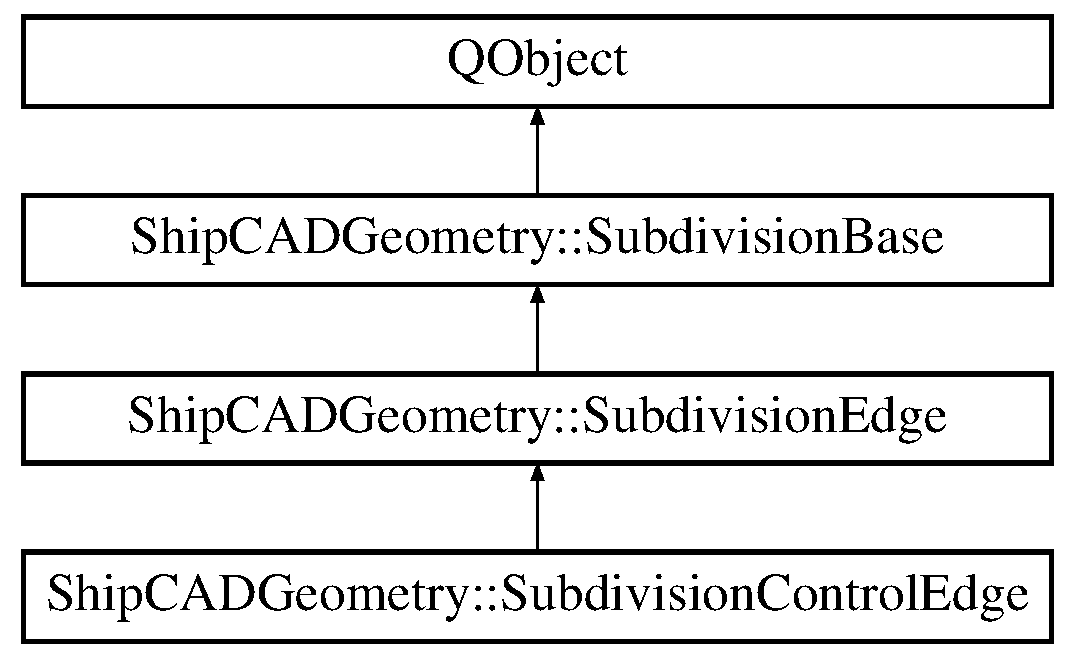
\includegraphics[height=4.000000cm]{classShipCADGeometry_1_1SubdivisionControlEdge}
\end{center}
\end{figure}
\subsection*{Public Member Functions}
\begin{DoxyCompactItemize}
\item 
\hyperlink{classShipCADGeometry_1_1SubdivisionControlEdge_aca48edfc1bb45a645708aecc8c8c3e04}{Subdivision\-Control\-Edge} (\hyperlink{classShipCADGeometry_1_1SubdivisionSurface}{Subdivision\-Surface} $\ast$owner)
\item 
virtual \hyperlink{classShipCADGeometry_1_1SubdivisionControlEdge_ad5e8153693c900a598618277cdeccd15}{$\sim$\-Subdivision\-Control\-Edge} ()
\item 
void \hyperlink{classShipCADGeometry_1_1SubdivisionControlEdge_a33fffac08b512f73c0676a5cfa81511d}{collapse} ()
\item 
\hyperlink{classShipCADGeometry_1_1SubdivisionControlPoint}{Subdivision\-Control\-Point} $\ast$ \hyperlink{classShipCADGeometry_1_1SubdivisionControlEdge_a4839a04d67e4240b570fd23be711bc10}{insert\-Control\-Point} (const Q\-Vector3\-D \&p)
\item 
void \hyperlink{classShipCADGeometry_1_1SubdivisionControlEdge_a07c67ddff486dc5e4ad830f549b32099}{trace} ()
\item 
size\-\_\-t \hyperlink{classShipCADGeometry_1_1SubdivisionControlEdge_a0fb224ed7895deb9eb4cdb57ab9c451c}{get\-Index} ()
\item 
Q\-Color \hyperlink{classShipCADGeometry_1_1SubdivisionControlEdge_a5cafa9a1fd8c93f10e2ae767608dfb26}{get\-Color} ()
\item 
virtual bool \hyperlink{classShipCADGeometry_1_1SubdivisionControlEdge_a23adc8ad28860987b7b4866eada3c463}{is\-Boundary\-Edge} ()
\item 
bool \hyperlink{classShipCADGeometry_1_1SubdivisionControlEdge_abcb240992ffb5637363341dbfd7003c7}{is\-Selected} ()
\item 
void \hyperlink{classShipCADGeometry_1_1SubdivisionControlEdge_ae247e08eec97952d1835df03c8269829}{set\-Selected} (bool val)
\item 
bool \hyperlink{classShipCADGeometry_1_1SubdivisionControlEdge_aaf83103b6772bf2387641b09194b12a6}{is\-Visible} ()
\item 
virtual void \hyperlink{classShipCADGeometry_1_1SubdivisionControlEdge_a6b86017a5ea7fe487f6017071406e8c4}{draw} (\hyperlink{classShipCADGeometry_1_1Viewport}{Viewport} \&vp, \hyperlink{classShipCADGeometry_1_1LineShader}{Line\-Shader} $\ast$lineshader)
\item 
void \hyperlink{classShipCADGeometry_1_1SubdivisionControlEdge_a0f48c4ce176a5de42e0a7c741aa129f5}{load\-Binary} (\hyperlink{classShipCADGeometry_1_1FileBuffer}{File\-Buffer} \&source)
\item 
void \hyperlink{classShipCADGeometry_1_1SubdivisionControlEdge_a572f4331ef0ab6f241583fc8d36cb93e}{save\-Binary} (\hyperlink{classShipCADGeometry_1_1FileBuffer}{File\-Buffer} \&destination)
\item 
void \hyperlink{classShipCADGeometry_1_1SubdivisionControlEdge_a7c6098254d4a92c44d01c3e247b29782}{load\-From\-Stream} (size\-\_\-t \&lineno, std\-::vector$<$ Q\-String $>$ \&strings)
\item 
void \hyperlink{classShipCADGeometry_1_1SubdivisionControlEdge_a21c0e8b4d4cd138ddd0bbcc707775040}{save\-To\-Stream} (std\-::vector$<$ Q\-String $>$ \&strings)
\item 
virtual void \hyperlink{classShipCADGeometry_1_1SubdivisionControlEdge_abdfa96ff05eff404214a92d38d7eb715}{dump} (std\-::ostream \&os, const char $\ast$prefix=\char`\"{}\char`\"{}) const 
\end{DoxyCompactItemize}
\subsection*{Static Public Member Functions}
\begin{DoxyCompactItemize}
\item 
static \hyperlink{classShipCADGeometry_1_1SubdivisionControlEdge}{Subdivision\-Control\-Edge} $\ast$ \hyperlink{classShipCADGeometry_1_1SubdivisionControlEdge_a20fc507b201766b6e3d0560595946fac}{construct} (\hyperlink{classShipCADGeometry_1_1SubdivisionSurface}{Subdivision\-Surface} $\ast$owner)
\end{DoxyCompactItemize}
\subsection*{Protected Member Functions}
\begin{DoxyCompactItemize}
\item 
void \hyperlink{classShipCADGeometry_1_1SubdivisionControlEdge_acc4cee57db50beb1dcc6361f7f2c62af}{priv\-\_\-dump} (std\-::ostream \&os, const char $\ast$prefix) const 
\item 
void \hyperlink{classShipCADGeometry_1_1SubdivisionControlEdge_aec6ff8caa6996ae5a9d2e58d5d2b0344}{priv\-\_\-trace} (\hyperlink{classShipCADGeometry_1_1SubdivisionControlPoint}{Subdivision\-Control\-Point} $\ast$p)
\end{DoxyCompactItemize}
\subsection*{Protected Attributes}
\begin{DoxyCompactItemize}
\item 
bool \hyperlink{classShipCADGeometry_1_1SubdivisionControlEdge_a64a6ff2aeb12cb4cba78290e61e164b9}{\-\_\-selected}
\item 
bool \hyperlink{classShipCADGeometry_1_1SubdivisionControlEdge_ad89cd12cf61e68944d709ee433c9d7ca}{\-\_\-visible}
\end{DoxyCompactItemize}
\subsection*{Properties}
\begin{DoxyCompactItemize}
\item 
Q\-Color \hyperlink{classShipCADGeometry_1_1SubdivisionControlEdge_a81cec7ea15307ae2e21cfcc238a059bb}{Color}
\item 
bool \hyperlink{classShipCADGeometry_1_1SubdivisionControlEdge_ae0d06a7dc36895347443a4c236bc1ea8}{Visible}
\item 
bool \hyperlink{classShipCADGeometry_1_1SubdivisionControlEdge_a6e4209c11ad0d122a6c4465790d2b7e3}{Selected}
\end{DoxyCompactItemize}


\subsection{Detailed Description}


Definition at line 119 of file subdivedge.\-h.



\subsection{Constructor \& Destructor Documentation}
\hypertarget{classShipCADGeometry_1_1SubdivisionControlEdge_aca48edfc1bb45a645708aecc8c8c3e04}{\index{Ship\-C\-A\-D\-Geometry\-::\-Subdivision\-Control\-Edge@{Ship\-C\-A\-D\-Geometry\-::\-Subdivision\-Control\-Edge}!Subdivision\-Control\-Edge@{Subdivision\-Control\-Edge}}
\index{Subdivision\-Control\-Edge@{Subdivision\-Control\-Edge}!ShipCADGeometry::SubdivisionControlEdge@{Ship\-C\-A\-D\-Geometry\-::\-Subdivision\-Control\-Edge}}
\subsubsection[{Subdivision\-Control\-Edge}]{\setlength{\rightskip}{0pt plus 5cm}Subdivision\-Control\-Edge\-::\-Subdivision\-Control\-Edge (
\begin{DoxyParamCaption}
\item[{{\bf Subdivision\-Surface} $\ast$}]{owner}
\end{DoxyParamCaption}
)\hspace{0.3cm}{\ttfamily [explicit]}}}\label{classShipCADGeometry_1_1SubdivisionControlEdge_aca48edfc1bb45a645708aecc8c8c3e04}


Definition at line 377 of file subdivedge.\-cpp.

\hypertarget{classShipCADGeometry_1_1SubdivisionControlEdge_ad5e8153693c900a598618277cdeccd15}{\index{Ship\-C\-A\-D\-Geometry\-::\-Subdivision\-Control\-Edge@{Ship\-C\-A\-D\-Geometry\-::\-Subdivision\-Control\-Edge}!$\sim$\-Subdivision\-Control\-Edge@{$\sim$\-Subdivision\-Control\-Edge}}
\index{$\sim$\-Subdivision\-Control\-Edge@{$\sim$\-Subdivision\-Control\-Edge}!ShipCADGeometry::SubdivisionControlEdge@{Ship\-C\-A\-D\-Geometry\-::\-Subdivision\-Control\-Edge}}
\subsubsection[{$\sim$\-Subdivision\-Control\-Edge}]{\setlength{\rightskip}{0pt plus 5cm}Subdivision\-Control\-Edge\-::$\sim$\-Subdivision\-Control\-Edge (
\begin{DoxyParamCaption}
{}
\end{DoxyParamCaption}
)\hspace{0.3cm}{\ttfamily [virtual]}}}\label{classShipCADGeometry_1_1SubdivisionControlEdge_ad5e8153693c900a598618277cdeccd15}


Definition at line 384 of file subdivedge.\-cpp.



\subsection{Member Function Documentation}
\hypertarget{classShipCADGeometry_1_1SubdivisionControlEdge_a33fffac08b512f73c0676a5cfa81511d}{\index{Ship\-C\-A\-D\-Geometry\-::\-Subdivision\-Control\-Edge@{Ship\-C\-A\-D\-Geometry\-::\-Subdivision\-Control\-Edge}!collapse@{collapse}}
\index{collapse@{collapse}!ShipCADGeometry::SubdivisionControlEdge@{Ship\-C\-A\-D\-Geometry\-::\-Subdivision\-Control\-Edge}}
\subsubsection[{collapse}]{\setlength{\rightskip}{0pt plus 5cm}void Subdivision\-Control\-Edge\-::collapse (
\begin{DoxyParamCaption}
{}
\end{DoxyParamCaption}
)}}\label{classShipCADGeometry_1_1SubdivisionControlEdge_a33fffac08b512f73c0676a5cfa81511d}


Definition at line 408 of file subdivedge.\-cpp.

\hypertarget{classShipCADGeometry_1_1SubdivisionControlEdge_a20fc507b201766b6e3d0560595946fac}{\index{Ship\-C\-A\-D\-Geometry\-::\-Subdivision\-Control\-Edge@{Ship\-C\-A\-D\-Geometry\-::\-Subdivision\-Control\-Edge}!construct@{construct}}
\index{construct@{construct}!ShipCADGeometry::SubdivisionControlEdge@{Ship\-C\-A\-D\-Geometry\-::\-Subdivision\-Control\-Edge}}
\subsubsection[{construct}]{\setlength{\rightskip}{0pt plus 5cm}{\bf Subdivision\-Control\-Edge} $\ast$ Subdivision\-Control\-Edge\-::construct (
\begin{DoxyParamCaption}
\item[{{\bf Subdivision\-Surface} $\ast$}]{owner}
\end{DoxyParamCaption}
)\hspace{0.3cm}{\ttfamily [static]}}}\label{classShipCADGeometry_1_1SubdivisionControlEdge_a20fc507b201766b6e3d0560595946fac}


Definition at line 369 of file subdivedge.\-cpp.

\hypertarget{classShipCADGeometry_1_1SubdivisionControlEdge_a6b86017a5ea7fe487f6017071406e8c4}{\index{Ship\-C\-A\-D\-Geometry\-::\-Subdivision\-Control\-Edge@{Ship\-C\-A\-D\-Geometry\-::\-Subdivision\-Control\-Edge}!draw@{draw}}
\index{draw@{draw}!ShipCADGeometry::SubdivisionControlEdge@{Ship\-C\-A\-D\-Geometry\-::\-Subdivision\-Control\-Edge}}
\subsubsection[{draw}]{\setlength{\rightskip}{0pt plus 5cm}void Subdivision\-Control\-Edge\-::draw (
\begin{DoxyParamCaption}
\item[{{\bf Viewport} \&}]{vp, }
\item[{{\bf Line\-Shader} $\ast$}]{lineshader}
\end{DoxyParamCaption}
)\hspace{0.3cm}{\ttfamily [virtual]}}}\label{classShipCADGeometry_1_1SubdivisionControlEdge_a6b86017a5ea7fe487f6017071406e8c4}


Definition at line 743 of file subdivedge.\-cpp.

\hypertarget{classShipCADGeometry_1_1SubdivisionControlEdge_abdfa96ff05eff404214a92d38d7eb715}{\index{Ship\-C\-A\-D\-Geometry\-::\-Subdivision\-Control\-Edge@{Ship\-C\-A\-D\-Geometry\-::\-Subdivision\-Control\-Edge}!dump@{dump}}
\index{dump@{dump}!ShipCADGeometry::SubdivisionControlEdge@{Ship\-C\-A\-D\-Geometry\-::\-Subdivision\-Control\-Edge}}
\subsubsection[{dump}]{\setlength{\rightskip}{0pt plus 5cm}void Subdivision\-Control\-Edge\-::dump (
\begin{DoxyParamCaption}
\item[{std\-::ostream \&}]{os, }
\item[{const char $\ast$}]{prefix = {\ttfamily \char`\"{}\char`\"{}}}
\end{DoxyParamCaption}
) const\hspace{0.3cm}{\ttfamily [virtual]}}}\label{classShipCADGeometry_1_1SubdivisionControlEdge_abdfa96ff05eff404214a92d38d7eb715}


Reimplemented from \hyperlink{classShipCADGeometry_1_1SubdivisionEdge_a14cc58877644ebd7b7ebffbdf8ef87f7}{Ship\-C\-A\-D\-Geometry\-::\-Subdivision\-Edge}.



Definition at line 810 of file subdivedge.\-cpp.

\hypertarget{classShipCADGeometry_1_1SubdivisionControlEdge_a5cafa9a1fd8c93f10e2ae767608dfb26}{\index{Ship\-C\-A\-D\-Geometry\-::\-Subdivision\-Control\-Edge@{Ship\-C\-A\-D\-Geometry\-::\-Subdivision\-Control\-Edge}!get\-Color@{get\-Color}}
\index{get\-Color@{get\-Color}!ShipCADGeometry::SubdivisionControlEdge@{Ship\-C\-A\-D\-Geometry\-::\-Subdivision\-Control\-Edge}}
\subsubsection[{get\-Color}]{\setlength{\rightskip}{0pt plus 5cm}Q\-Color Subdivision\-Control\-Edge\-::get\-Color (
\begin{DoxyParamCaption}
{}
\end{DoxyParamCaption}
)}}\label{classShipCADGeometry_1_1SubdivisionControlEdge_a5cafa9a1fd8c93f10e2ae767608dfb26}


Definition at line 531 of file subdivedge.\-cpp.

\hypertarget{classShipCADGeometry_1_1SubdivisionControlEdge_a0fb224ed7895deb9eb4cdb57ab9c451c}{\index{Ship\-C\-A\-D\-Geometry\-::\-Subdivision\-Control\-Edge@{Ship\-C\-A\-D\-Geometry\-::\-Subdivision\-Control\-Edge}!get\-Index@{get\-Index}}
\index{get\-Index@{get\-Index}!ShipCADGeometry::SubdivisionControlEdge@{Ship\-C\-A\-D\-Geometry\-::\-Subdivision\-Control\-Edge}}
\subsubsection[{get\-Index}]{\setlength{\rightskip}{0pt plus 5cm}size\-\_\-t Subdivision\-Control\-Edge\-::get\-Index (
\begin{DoxyParamCaption}
{}
\end{DoxyParamCaption}
)}}\label{classShipCADGeometry_1_1SubdivisionControlEdge_a0fb224ed7895deb9eb4cdb57ab9c451c}


Definition at line 545 of file subdivedge.\-cpp.

\hypertarget{classShipCADGeometry_1_1SubdivisionControlEdge_a4839a04d67e4240b570fd23be711bc10}{\index{Ship\-C\-A\-D\-Geometry\-::\-Subdivision\-Control\-Edge@{Ship\-C\-A\-D\-Geometry\-::\-Subdivision\-Control\-Edge}!insert\-Control\-Point@{insert\-Control\-Point}}
\index{insert\-Control\-Point@{insert\-Control\-Point}!ShipCADGeometry::SubdivisionControlEdge@{Ship\-C\-A\-D\-Geometry\-::\-Subdivision\-Control\-Edge}}
\subsubsection[{insert\-Control\-Point}]{\setlength{\rightskip}{0pt plus 5cm}{\bf Subdivision\-Control\-Point} $\ast$ Subdivision\-Control\-Edge\-::insert\-Control\-Point (
\begin{DoxyParamCaption}
\item[{const Q\-Vector3\-D \&}]{p}
\end{DoxyParamCaption}
)}}\label{classShipCADGeometry_1_1SubdivisionControlEdge_a4839a04d67e4240b570fd23be711bc10}


Definition at line 606 of file subdivedge.\-cpp.

\hypertarget{classShipCADGeometry_1_1SubdivisionControlEdge_a23adc8ad28860987b7b4866eada3c463}{\index{Ship\-C\-A\-D\-Geometry\-::\-Subdivision\-Control\-Edge@{Ship\-C\-A\-D\-Geometry\-::\-Subdivision\-Control\-Edge}!is\-Boundary\-Edge@{is\-Boundary\-Edge}}
\index{is\-Boundary\-Edge@{is\-Boundary\-Edge}!ShipCADGeometry::SubdivisionControlEdge@{Ship\-C\-A\-D\-Geometry\-::\-Subdivision\-Control\-Edge}}
\subsubsection[{is\-Boundary\-Edge}]{\setlength{\rightskip}{0pt plus 5cm}bool Subdivision\-Control\-Edge\-::is\-Boundary\-Edge (
\begin{DoxyParamCaption}
{}
\end{DoxyParamCaption}
)\hspace{0.3cm}{\ttfamily [virtual]}}}\label{classShipCADGeometry_1_1SubdivisionControlEdge_a23adc8ad28860987b7b4866eada3c463}


Reimplemented from \hyperlink{classShipCADGeometry_1_1SubdivisionEdge_ad95a3ec8ba66deb74cbfd3d36428fc34}{Ship\-C\-A\-D\-Geometry\-::\-Subdivision\-Edge}.



Definition at line 550 of file subdivedge.\-cpp.

\hypertarget{classShipCADGeometry_1_1SubdivisionControlEdge_abcb240992ffb5637363341dbfd7003c7}{\index{Ship\-C\-A\-D\-Geometry\-::\-Subdivision\-Control\-Edge@{Ship\-C\-A\-D\-Geometry\-::\-Subdivision\-Control\-Edge}!is\-Selected@{is\-Selected}}
\index{is\-Selected@{is\-Selected}!ShipCADGeometry::SubdivisionControlEdge@{Ship\-C\-A\-D\-Geometry\-::\-Subdivision\-Control\-Edge}}
\subsubsection[{is\-Selected}]{\setlength{\rightskip}{0pt plus 5cm}bool Subdivision\-Control\-Edge\-::is\-Selected (
\begin{DoxyParamCaption}
{}
\end{DoxyParamCaption}
)}}\label{classShipCADGeometry_1_1SubdivisionControlEdge_abcb240992ffb5637363341dbfd7003c7}


Definition at line 573 of file subdivedge.\-cpp.

\hypertarget{classShipCADGeometry_1_1SubdivisionControlEdge_aaf83103b6772bf2387641b09194b12a6}{\index{Ship\-C\-A\-D\-Geometry\-::\-Subdivision\-Control\-Edge@{Ship\-C\-A\-D\-Geometry\-::\-Subdivision\-Control\-Edge}!is\-Visible@{is\-Visible}}
\index{is\-Visible@{is\-Visible}!ShipCADGeometry::SubdivisionControlEdge@{Ship\-C\-A\-D\-Geometry\-::\-Subdivision\-Control\-Edge}}
\subsubsection[{is\-Visible}]{\setlength{\rightskip}{0pt plus 5cm}bool Subdivision\-Control\-Edge\-::is\-Visible (
\begin{DoxyParamCaption}
{}
\end{DoxyParamCaption}
)}}\label{classShipCADGeometry_1_1SubdivisionControlEdge_aaf83103b6772bf2387641b09194b12a6}


Definition at line 578 of file subdivedge.\-cpp.

\hypertarget{classShipCADGeometry_1_1SubdivisionControlEdge_a0f48c4ce176a5de42e0a7c741aa129f5}{\index{Ship\-C\-A\-D\-Geometry\-::\-Subdivision\-Control\-Edge@{Ship\-C\-A\-D\-Geometry\-::\-Subdivision\-Control\-Edge}!load\-Binary@{load\-Binary}}
\index{load\-Binary@{load\-Binary}!ShipCADGeometry::SubdivisionControlEdge@{Ship\-C\-A\-D\-Geometry\-::\-Subdivision\-Control\-Edge}}
\subsubsection[{load\-Binary}]{\setlength{\rightskip}{0pt plus 5cm}void Subdivision\-Control\-Edge\-::load\-Binary (
\begin{DoxyParamCaption}
\item[{{\bf File\-Buffer} \&}]{source}
\end{DoxyParamCaption}
)}}\label{classShipCADGeometry_1_1SubdivisionControlEdge_a0f48c4ce176a5de42e0a7c741aa129f5}


Definition at line 648 of file subdivedge.\-cpp.

\hypertarget{classShipCADGeometry_1_1SubdivisionControlEdge_a7c6098254d4a92c44d01c3e247b29782}{\index{Ship\-C\-A\-D\-Geometry\-::\-Subdivision\-Control\-Edge@{Ship\-C\-A\-D\-Geometry\-::\-Subdivision\-Control\-Edge}!load\-From\-Stream@{load\-From\-Stream}}
\index{load\-From\-Stream@{load\-From\-Stream}!ShipCADGeometry::SubdivisionControlEdge@{Ship\-C\-A\-D\-Geometry\-::\-Subdivision\-Control\-Edge}}
\subsubsection[{load\-From\-Stream}]{\setlength{\rightskip}{0pt plus 5cm}void Subdivision\-Control\-Edge\-::load\-From\-Stream (
\begin{DoxyParamCaption}
\item[{size\-\_\-t \&}]{lineno, }
\item[{std\-::vector$<$ Q\-String $>$ \&}]{strings}
\end{DoxyParamCaption}
)}}\label{classShipCADGeometry_1_1SubdivisionControlEdge_a7c6098254d4a92c44d01c3e247b29782}


Definition at line 666 of file subdivedge.\-cpp.

\hypertarget{classShipCADGeometry_1_1SubdivisionControlEdge_acc4cee57db50beb1dcc6361f7f2c62af}{\index{Ship\-C\-A\-D\-Geometry\-::\-Subdivision\-Control\-Edge@{Ship\-C\-A\-D\-Geometry\-::\-Subdivision\-Control\-Edge}!priv\-\_\-dump@{priv\-\_\-dump}}
\index{priv\-\_\-dump@{priv\-\_\-dump}!ShipCADGeometry::SubdivisionControlEdge@{Ship\-C\-A\-D\-Geometry\-::\-Subdivision\-Control\-Edge}}
\subsubsection[{priv\-\_\-dump}]{\setlength{\rightskip}{0pt plus 5cm}void Subdivision\-Control\-Edge\-::priv\-\_\-dump (
\begin{DoxyParamCaption}
\item[{std\-::ostream \&}]{os, }
\item[{const char $\ast$}]{prefix}
\end{DoxyParamCaption}
) const\hspace{0.3cm}{\ttfamily [protected]}}}\label{classShipCADGeometry_1_1SubdivisionControlEdge_acc4cee57db50beb1dcc6361f7f2c62af}


Definition at line 818 of file subdivedge.\-cpp.

\hypertarget{classShipCADGeometry_1_1SubdivisionControlEdge_aec6ff8caa6996ae5a9d2e58d5d2b0344}{\index{Ship\-C\-A\-D\-Geometry\-::\-Subdivision\-Control\-Edge@{Ship\-C\-A\-D\-Geometry\-::\-Subdivision\-Control\-Edge}!priv\-\_\-trace@{priv\-\_\-trace}}
\index{priv\-\_\-trace@{priv\-\_\-trace}!ShipCADGeometry::SubdivisionControlEdge@{Ship\-C\-A\-D\-Geometry\-::\-Subdivision\-Control\-Edge}}
\subsubsection[{priv\-\_\-trace}]{\setlength{\rightskip}{0pt plus 5cm}void Subdivision\-Control\-Edge\-::priv\-\_\-trace (
\begin{DoxyParamCaption}
\item[{{\bf Subdivision\-Control\-Point} $\ast$}]{p}
\end{DoxyParamCaption}
)\hspace{0.3cm}{\ttfamily [protected]}}}\label{classShipCADGeometry_1_1SubdivisionControlEdge_aec6ff8caa6996ae5a9d2e58d5d2b0344}


Definition at line 704 of file subdivedge.\-cpp.

\hypertarget{classShipCADGeometry_1_1SubdivisionControlEdge_a572f4331ef0ab6f241583fc8d36cb93e}{\index{Ship\-C\-A\-D\-Geometry\-::\-Subdivision\-Control\-Edge@{Ship\-C\-A\-D\-Geometry\-::\-Subdivision\-Control\-Edge}!save\-Binary@{save\-Binary}}
\index{save\-Binary@{save\-Binary}!ShipCADGeometry::SubdivisionControlEdge@{Ship\-C\-A\-D\-Geometry\-::\-Subdivision\-Control\-Edge}}
\subsubsection[{save\-Binary}]{\setlength{\rightskip}{0pt plus 5cm}void Subdivision\-Control\-Edge\-::save\-Binary (
\begin{DoxyParamCaption}
\item[{{\bf File\-Buffer} \&}]{destination}
\end{DoxyParamCaption}
)}}\label{classShipCADGeometry_1_1SubdivisionControlEdge_a572f4331ef0ab6f241583fc8d36cb93e}


Definition at line 696 of file subdivedge.\-cpp.

\hypertarget{classShipCADGeometry_1_1SubdivisionControlEdge_a21c0e8b4d4cd138ddd0bbcc707775040}{\index{Ship\-C\-A\-D\-Geometry\-::\-Subdivision\-Control\-Edge@{Ship\-C\-A\-D\-Geometry\-::\-Subdivision\-Control\-Edge}!save\-To\-Stream@{save\-To\-Stream}}
\index{save\-To\-Stream@{save\-To\-Stream}!ShipCADGeometry::SubdivisionControlEdge@{Ship\-C\-A\-D\-Geometry\-::\-Subdivision\-Control\-Edge}}
\subsubsection[{save\-To\-Stream}]{\setlength{\rightskip}{0pt plus 5cm}void Subdivision\-Control\-Edge\-::save\-To\-Stream (
\begin{DoxyParamCaption}
\item[{std\-::vector$<$ Q\-String $>$ \&}]{strings}
\end{DoxyParamCaption}
)}}\label{classShipCADGeometry_1_1SubdivisionControlEdge_a21c0e8b4d4cd138ddd0bbcc707775040}


Definition at line 686 of file subdivedge.\-cpp.

\hypertarget{classShipCADGeometry_1_1SubdivisionControlEdge_ae247e08eec97952d1835df03c8269829}{\index{Ship\-C\-A\-D\-Geometry\-::\-Subdivision\-Control\-Edge@{Ship\-C\-A\-D\-Geometry\-::\-Subdivision\-Control\-Edge}!set\-Selected@{set\-Selected}}
\index{set\-Selected@{set\-Selected}!ShipCADGeometry::SubdivisionControlEdge@{Ship\-C\-A\-D\-Geometry\-::\-Subdivision\-Control\-Edge}}
\subsubsection[{set\-Selected}]{\setlength{\rightskip}{0pt plus 5cm}void Subdivision\-Control\-Edge\-::set\-Selected (
\begin{DoxyParamCaption}
\item[{bool}]{val}
\end{DoxyParamCaption}
)}}\label{classShipCADGeometry_1_1SubdivisionControlEdge_ae247e08eec97952d1835df03c8269829}


Definition at line 565 of file subdivedge.\-cpp.

\hypertarget{classShipCADGeometry_1_1SubdivisionControlEdge_a07c67ddff486dc5e4ad830f549b32099}{\index{Ship\-C\-A\-D\-Geometry\-::\-Subdivision\-Control\-Edge@{Ship\-C\-A\-D\-Geometry\-::\-Subdivision\-Control\-Edge}!trace@{trace}}
\index{trace@{trace}!ShipCADGeometry::SubdivisionControlEdge@{Ship\-C\-A\-D\-Geometry\-::\-Subdivision\-Control\-Edge}}
\subsubsection[{trace}]{\setlength{\rightskip}{0pt plus 5cm}void Subdivision\-Control\-Edge\-::trace (
\begin{DoxyParamCaption}
{}
\end{DoxyParamCaption}
)}}\label{classShipCADGeometry_1_1SubdivisionControlEdge_a07c67ddff486dc5e4ad830f549b32099}


Definition at line 733 of file subdivedge.\-cpp.



\subsection{Member Data Documentation}
\hypertarget{classShipCADGeometry_1_1SubdivisionControlEdge_a64a6ff2aeb12cb4cba78290e61e164b9}{\index{Ship\-C\-A\-D\-Geometry\-::\-Subdivision\-Control\-Edge@{Ship\-C\-A\-D\-Geometry\-::\-Subdivision\-Control\-Edge}!\-\_\-selected@{\-\_\-selected}}
\index{\-\_\-selected@{\-\_\-selected}!ShipCADGeometry::SubdivisionControlEdge@{Ship\-C\-A\-D\-Geometry\-::\-Subdivision\-Control\-Edge}}
\subsubsection[{\-\_\-selected}]{\setlength{\rightskip}{0pt plus 5cm}bool Ship\-C\-A\-D\-Geometry\-::\-Subdivision\-Control\-Edge\-::\-\_\-selected\hspace{0.3cm}{\ttfamily [protected]}}}\label{classShipCADGeometry_1_1SubdivisionControlEdge_a64a6ff2aeb12cb4cba78290e61e164b9}


Definition at line 166 of file subdivedge.\-h.

\hypertarget{classShipCADGeometry_1_1SubdivisionControlEdge_ad89cd12cf61e68944d709ee433c9d7ca}{\index{Ship\-C\-A\-D\-Geometry\-::\-Subdivision\-Control\-Edge@{Ship\-C\-A\-D\-Geometry\-::\-Subdivision\-Control\-Edge}!\-\_\-visible@{\-\_\-visible}}
\index{\-\_\-visible@{\-\_\-visible}!ShipCADGeometry::SubdivisionControlEdge@{Ship\-C\-A\-D\-Geometry\-::\-Subdivision\-Control\-Edge}}
\subsubsection[{\-\_\-visible}]{\setlength{\rightskip}{0pt plus 5cm}bool Ship\-C\-A\-D\-Geometry\-::\-Subdivision\-Control\-Edge\-::\-\_\-visible\hspace{0.3cm}{\ttfamily [protected]}}}\label{classShipCADGeometry_1_1SubdivisionControlEdge_ad89cd12cf61e68944d709ee433c9d7ca}


Definition at line 167 of file subdivedge.\-h.



\subsection{Property Documentation}
\hypertarget{classShipCADGeometry_1_1SubdivisionControlEdge_a81cec7ea15307ae2e21cfcc238a059bb}{\index{Ship\-C\-A\-D\-Geometry\-::\-Subdivision\-Control\-Edge@{Ship\-C\-A\-D\-Geometry\-::\-Subdivision\-Control\-Edge}!Color@{Color}}
\index{Color@{Color}!ShipCADGeometry::SubdivisionControlEdge@{Ship\-C\-A\-D\-Geometry\-::\-Subdivision\-Control\-Edge}}
\subsubsection[{Color}]{\setlength{\rightskip}{0pt plus 5cm}Q\-Color Ship\-C\-A\-D\-Geometry\-::\-Subdivision\-Control\-Edge\-::\-Color\hspace{0.3cm}{\ttfamily [read]}}}\label{classShipCADGeometry_1_1SubdivisionControlEdge_a81cec7ea15307ae2e21cfcc238a059bb}


Definition at line 122 of file subdivedge.\-h.

\hypertarget{classShipCADGeometry_1_1SubdivisionControlEdge_a6e4209c11ad0d122a6c4465790d2b7e3}{\index{Ship\-C\-A\-D\-Geometry\-::\-Subdivision\-Control\-Edge@{Ship\-C\-A\-D\-Geometry\-::\-Subdivision\-Control\-Edge}!Selected@{Selected}}
\index{Selected@{Selected}!ShipCADGeometry::SubdivisionControlEdge@{Ship\-C\-A\-D\-Geometry\-::\-Subdivision\-Control\-Edge}}
\subsubsection[{Selected}]{\setlength{\rightskip}{0pt plus 5cm}bool Ship\-C\-A\-D\-Geometry\-::\-Subdivision\-Control\-Edge\-::\-Selected\hspace{0.3cm}{\ttfamily [read]}, {\ttfamily [write]}}}\label{classShipCADGeometry_1_1SubdivisionControlEdge_a6e4209c11ad0d122a6c4465790d2b7e3}


Definition at line 124 of file subdivedge.\-h.

\hypertarget{classShipCADGeometry_1_1SubdivisionControlEdge_ae0d06a7dc36895347443a4c236bc1ea8}{\index{Ship\-C\-A\-D\-Geometry\-::\-Subdivision\-Control\-Edge@{Ship\-C\-A\-D\-Geometry\-::\-Subdivision\-Control\-Edge}!Visible@{Visible}}
\index{Visible@{Visible}!ShipCADGeometry::SubdivisionControlEdge@{Ship\-C\-A\-D\-Geometry\-::\-Subdivision\-Control\-Edge}}
\subsubsection[{Visible}]{\setlength{\rightskip}{0pt plus 5cm}bool Ship\-C\-A\-D\-Geometry\-::\-Subdivision\-Control\-Edge\-::\-Visible\hspace{0.3cm}{\ttfamily [read]}}}\label{classShipCADGeometry_1_1SubdivisionControlEdge_ae0d06a7dc36895347443a4c236bc1ea8}


Definition at line 123 of file subdivedge.\-h.



The documentation for this class was generated from the following files\-:\begin{DoxyCompactItemize}
\item 
Ship\-C\-A\-Dlib/\hyperlink{subdivedge_8h}{subdivedge.\-h}\item 
Ship\-C\-A\-Dlib/\hyperlink{subdivedge_8cpp}{subdivedge.\-cpp}\end{DoxyCompactItemize}

\hypertarget{classShipCADGeometry_1_1SubdivisionControlFace}{\section{Ship\-C\-A\-D\-Geometry\-:\-:Subdivision\-Control\-Face Class Reference}
\label{classShipCADGeometry_1_1SubdivisionControlFace}\index{Ship\-C\-A\-D\-Geometry\-::\-Subdivision\-Control\-Face@{Ship\-C\-A\-D\-Geometry\-::\-Subdivision\-Control\-Face}}
}


{\ttfamily \#include $<$subdivface.\-h$>$}

Inheritance diagram for Ship\-C\-A\-D\-Geometry\-:\-:Subdivision\-Control\-Face\-:\begin{figure}[H]
\begin{center}
\leavevmode
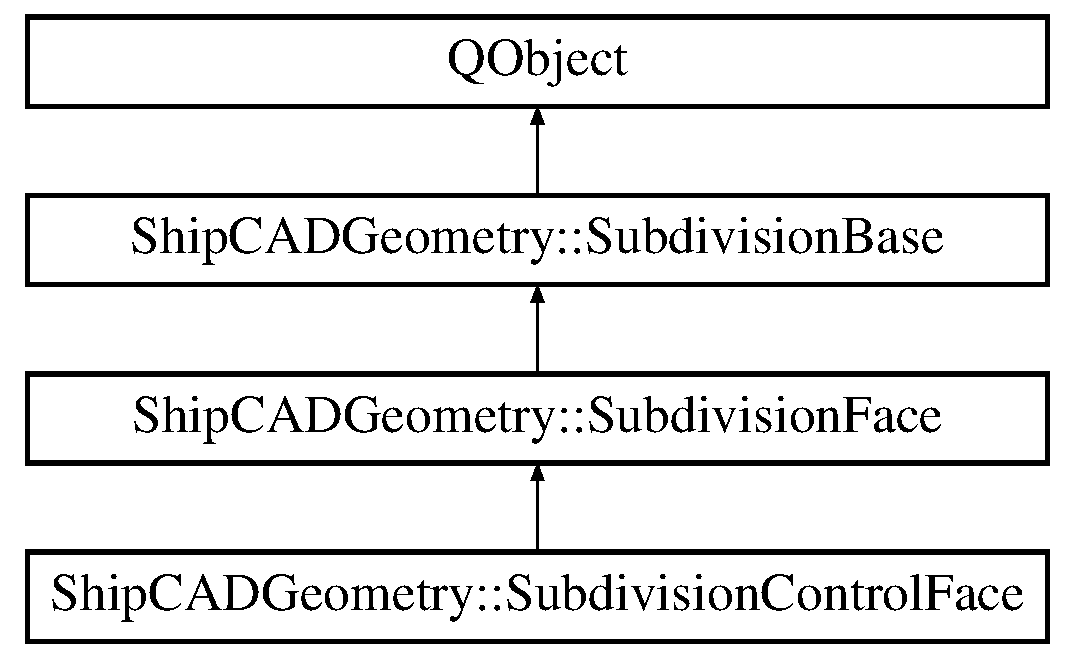
\includegraphics[height=4.000000cm]{classShipCADGeometry_1_1SubdivisionControlFace}
\end{center}
\end{figure}
\subsection*{Public Member Functions}
\begin{DoxyCompactItemize}
\item 
\hyperlink{classShipCADGeometry_1_1SubdivisionControlFace_a9316495869082b0e3e27092118913644}{Subdivision\-Control\-Face} (\hyperlink{classShipCADGeometry_1_1SubdivisionSurface}{Subdivision\-Surface} $\ast$owner)
\item 
virtual \hyperlink{classShipCADGeometry_1_1SubdivisionControlFace_a7b092e764ec2708674afdb210196f761}{$\sim$\-Subdivision\-Control\-Face} ()
\item 
void \hyperlink{classShipCADGeometry_1_1SubdivisionControlFace_a611c74ce3f346a745d4a694f5aab4ec2}{calc\-Extents} ()
\item 
virtual void \hyperlink{classShipCADGeometry_1_1SubdivisionControlFace_ad168e31f0ef2537b3cd0f58b0c1c54e2}{clear} ()
\begin{DoxyCompactList}\small\item\em reset this element to default values \end{DoxyCompactList}\item 
void \hyperlink{classShipCADGeometry_1_1SubdivisionControlFace_a1501212af025c7e33ede929d50a76651}{clear\-Children} ()
\item 
void \hyperlink{classShipCADGeometry_1_1SubdivisionControlFace_ad8d1c627c87a5f151610b446dd889bf7}{clear\-Control\-Edges} ()
\item 
\hyperlink{classShipCADGeometry_1_1SubdivisionControlEdge}{Subdivision\-Control\-Edge} $\ast$ \hyperlink{classShipCADGeometry_1_1SubdivisionControlFace_af585a1c8300791375b2df87fe2ebc4f5}{insert\-Control\-Edge} (\hyperlink{classShipCADGeometry_1_1SubdivisionControlPoint}{Subdivision\-Control\-Point} $\ast$p1, \hyperlink{classShipCADGeometry_1_1SubdivisionControlPoint}{Subdivision\-Control\-Point} $\ast$p2)
\item 
void \hyperlink{classShipCADGeometry_1_1SubdivisionControlFace_a1c5253075cbe1f05ba004bee4edb8698}{remove\-References} ()
\item 
virtual void \hyperlink{classShipCADGeometry_1_1SubdivisionControlFace_a2f4b7c97d87649d302ef512b1b8db707}{subdivide} (std\-::vector$<$ std\-::pair$<$ \hyperlink{classShipCADGeometry_1_1SubdivisionPoint}{Subdivision\-Point} $\ast$, \hyperlink{classShipCADGeometry_1_1SubdivisionPoint}{Subdivision\-Point} $\ast$ $>$ $>$ \&vertexpoints, std\-::vector$<$ std\-::pair$<$ \hyperlink{classShipCADGeometry_1_1SubdivisionEdge}{Subdivision\-Edge} $\ast$, \hyperlink{classShipCADGeometry_1_1SubdivisionPoint}{Subdivision\-Point} $\ast$ $>$ $>$ \&edgepoints, std\-::vector$<$ std\-::pair$<$ \hyperlink{classShipCADGeometry_1_1SubdivisionFace}{Subdivision\-Face} $\ast$, \hyperlink{classShipCADGeometry_1_1SubdivisionPoint}{Subdivision\-Point} $\ast$ $>$ $>$ \&facepoints, std\-::vector$<$ \hyperlink{classShipCADGeometry_1_1SubdivisionEdge}{Subdivision\-Edge} $\ast$ $>$ \&interioredges, std\-::vector$<$ \hyperlink{classShipCADGeometry_1_1SubdivisionEdge}{Subdivision\-Edge} $\ast$ $>$ \&controledges, std\-::vector$<$ \hyperlink{classShipCADGeometry_1_1SubdivisionFace}{Subdivision\-Face} $\ast$ $>$ \&dest)
\item 
void \hyperlink{classShipCADGeometry_1_1SubdivisionControlFace_a768d000d2891ca110d6eb804abf80351}{trace} ()
\item 
\hyperlink{classShipCADGeometry_1_1SubdivisionLayer}{Subdivision\-Layer} $\ast$ \hyperlink{classShipCADGeometry_1_1SubdivisionControlFace_a2e845cb5e4def22e7efe244ff6a3b168}{get\-Layer} ()
\item 
void \hyperlink{classShipCADGeometry_1_1SubdivisionControlFace_a23631dfffd1c3ad7fc59537a4684fa01}{set\-Layer} (\hyperlink{classShipCADGeometry_1_1SubdivisionLayer}{Subdivision\-Layer} $\ast$layer)
\item 
\hyperlink{classShipCADGeometry_1_1SubdivisionFace}{Subdivision\-Face} $\ast$ \hyperlink{classShipCADGeometry_1_1SubdivisionControlFace_a2c25793e1bed9472121e9126bacac3ce}{get\-Child} (size\-\_\-t index)
\item 
size\-\_\-t \hyperlink{classShipCADGeometry_1_1SubdivisionControlFace_abaa5b8839ae4b8907b4c00d279d3e002}{number\-Of\-Children} ()
\item 
Q\-Color \hyperlink{classShipCADGeometry_1_1SubdivisionControlFace_a8a350fe4fec2ee93228ed9400a6f145c}{get\-Color} ()
\item 
\hyperlink{classShipCADGeometry_1_1SubdivisionEdge}{Subdivision\-Edge} $\ast$ \hyperlink{classShipCADGeometry_1_1SubdivisionControlFace_accfc3e8e3d79a2303126e44e6fdb1728}{get\-Control\-Edge} (size\-\_\-t index)
\item 
size\-\_\-t \hyperlink{classShipCADGeometry_1_1SubdivisionControlFace_a6fd6ad99f4b1af14005936509e5cbbb2}{number\-Of\-Control\-Edges} ()
\item 
\hyperlink{classShipCADGeometry_1_1SubdivisionEdge}{Subdivision\-Edge} $\ast$ \hyperlink{classShipCADGeometry_1_1SubdivisionControlFace_a37af31abc48d84d607c15158ad7c6a2a}{get\-Edge} (size\-\_\-t index)
\item 
size\-\_\-t \hyperlink{classShipCADGeometry_1_1SubdivisionControlFace_a51e9bb7f8223daceba617bdae326b155}{number\-Of\-Edges} ()
\item 
size\-\_\-t \hyperlink{classShipCADGeometry_1_1SubdivisionControlFace_a72f906db976c6530f0f2d4c03701ad15}{get\-Index} ()
\item 
bool \hyperlink{classShipCADGeometry_1_1SubdivisionControlFace_ab56a2d4c3fccb7a578def71d286ee03c}{is\-Selected} ()
\item 
bool \hyperlink{classShipCADGeometry_1_1SubdivisionControlFace_a2a722717e127bac12e3b81f4664fc568}{is\-Visible} ()
\item 
void \hyperlink{classShipCADGeometry_1_1SubdivisionControlFace_a2ce580378cd200faec6a24d9d794c68e}{set\-Selected} (bool val)
\item 
Q\-Vector3\-D \hyperlink{classShipCADGeometry_1_1SubdivisionControlFace_a7206287dd23fe07ad6fb929258a15f01}{get\-Min} ()
\item 
Q\-Vector3\-D \hyperlink{classShipCADGeometry_1_1SubdivisionControlFace_a06eea7586cd4971162f6d9bc1d0852d8}{get\-Max} ()
\item 
std\-::vector$<$ \hyperlink{classShipCADGeometry_1_1SubdivisionFace}{Subdivision\-Face} $\ast$ $>$\\*
\-::iterator \hyperlink{classShipCADGeometry_1_1SubdivisionControlFace_ac6efdc9d144af407d9b044d82779f61f}{children\-Begin} ()
\item 
std\-::vector$<$ \hyperlink{classShipCADGeometry_1_1SubdivisionFace}{Subdivision\-Face} $\ast$ $>$\\*
\-::iterator \hyperlink{classShipCADGeometry_1_1SubdivisionControlFace_ac11e1779fe39e51a0fa7ae09165a9902}{children\-End} ()
\item 
void \hyperlink{classShipCADGeometry_1_1SubdivisionControlFace_aa5ba43707787cde6e99cd645708e9200}{load\-Binary} (\hyperlink{classShipCADGeometry_1_1FileBuffer}{File\-Buffer} \&source)
\item 
void \hyperlink{classShipCADGeometry_1_1SubdivisionControlFace_a562b877e868dbd86ffe2c864232e1b78}{save\-Binary} (\hyperlink{classShipCADGeometry_1_1FileBuffer}{File\-Buffer} \&destination)
\item 
void \hyperlink{classShipCADGeometry_1_1SubdivisionControlFace_ab2aaada5c28682e4f17bc47261203cee}{save\-To\-D\-X\-F} (std\-::vector$<$ Q\-String $>$ \&strings)
\item 
void \hyperlink{classShipCADGeometry_1_1SubdivisionControlFace_aa75c77ee2e007015851930a604744aa0}{save\-To\-Stream} (std\-::vector$<$ Q\-String $>$ \&strings)
\item 
void \hyperlink{classShipCADGeometry_1_1SubdivisionControlFace_ae856d93b8844854d908835df1f363ddd}{load\-From\-Stream} (size\-\_\-t \&lineno, std\-::vector$<$ Q\-String $>$ \&strings)
\item 
virtual void \hyperlink{classShipCADGeometry_1_1SubdivisionControlFace_ac253493bccd91108d936b651e72b46f8}{draw} (\hyperlink{classShipCADGeometry_1_1Viewport}{Viewport} \&vp, \hyperlink{classShipCADGeometry_1_1LineShader}{Line\-Shader} $\ast$lineshader)
\item 
virtual void \hyperlink{classShipCADGeometry_1_1SubdivisionControlFace_aef1327fd3e623b190d67dcb461a3e950}{draw\-Faces} (\hyperlink{classShipCADGeometry_1_1Viewport}{Viewport} \&vp, \hyperlink{classShipCADGeometry_1_1MonoFaceShader}{Mono\-Face\-Shader} $\ast$monoshader)
\item 
virtual void \hyperlink{classShipCADGeometry_1_1SubdivisionControlFace_aaf9226150996743d8d2ea560083ad1d8}{draw\-Curvature\-Faces} (\hyperlink{classShipCADGeometry_1_1Viewport}{Viewport} \&vp, float Min\-Curvature, float Max\-Curvature)
\item 
virtual void \hyperlink{classShipCADGeometry_1_1SubdivisionControlFace_a947868fba3e9bb6c587847fb9245c9ff}{dump} (std\-::ostream \&os, const char $\ast$prefix=\char`\"{}\char`\"{}) const 
\begin{DoxyCompactList}\small\item\em print out the element to a stream \end{DoxyCompactList}\end{DoxyCompactItemize}
\subsection*{Static Public Member Functions}
\begin{DoxyCompactItemize}
\item 
static \hyperlink{classShipCADGeometry_1_1SubdivisionControlFace}{Subdivision\-Control\-Face} $\ast$ \hyperlink{classShipCADGeometry_1_1SubdivisionControlFace_a4117f55ab3ec27bebd933f2992bc5dcd}{construct} (\hyperlink{classShipCADGeometry_1_1SubdivisionSurface}{Subdivision\-Surface} $\ast$owner)
\end{DoxyCompactItemize}
\subsection*{Protected Member Functions}
\begin{DoxyCompactItemize}
\item 
void \hyperlink{classShipCADGeometry_1_1SubdivisionControlFace_a224ce57a8d9d631eef63cccd8e0113f9}{priv\-\_\-dump} (std\-::ostream \&os, const char $\ast$prefix) const 
\item 
void \hyperlink{classShipCADGeometry_1_1SubdivisionControlFace_aa6035e53cd1e32a9bd9e9f9800c9f7d4}{find\-Attached\-Faces} (std\-::vector$<$ \hyperlink{classShipCADGeometry_1_1SubdivisionControlFace}{Subdivision\-Control\-Face} $\ast$ $>$ \&todo\-\_\-list, \hyperlink{classShipCADGeometry_1_1SubdivisionControlFace}{Subdivision\-Control\-Face} $\ast$face)
\end{DoxyCompactItemize}
\subsection*{Protected Attributes}
\begin{DoxyCompactItemize}
\item 
\hyperlink{classShipCADGeometry_1_1SubdivisionLayer}{Subdivision\-Layer} $\ast$ \hyperlink{classShipCADGeometry_1_1SubdivisionControlFace_a83e0b0518f2206f2ceccf1e9e9894f8d}{\-\_\-layer}
\item 
Q\-Vector3\-D \hyperlink{classShipCADGeometry_1_1SubdivisionControlFace_abc8afda2435ea3e2b8f7d66e04eede3d}{\-\_\-min}
\item 
Q\-Vector3\-D \hyperlink{classShipCADGeometry_1_1SubdivisionControlFace_ada4bdde0addfa469e49a36d1ac99bf00}{\-\_\-max}
\item 
std\-::vector$<$ \hyperlink{classShipCADGeometry_1_1SubdivisionFace}{Subdivision\-Face} $\ast$ $>$ \hyperlink{classShipCADGeometry_1_1SubdivisionControlFace_a241bcefc9f6727dec87f6a754f99cc3d}{\-\_\-children}
\item 
std\-::vector$<$ \hyperlink{classShipCADGeometry_1_1SubdivisionEdge}{Subdivision\-Edge} $\ast$ $>$ \hyperlink{classShipCADGeometry_1_1SubdivisionControlFace_a5efceb94118053e2d6ffdff45f68489e}{\-\_\-edges}
\item 
std\-::vector$<$ \hyperlink{classShipCADGeometry_1_1SubdivisionEdge}{Subdivision\-Edge} $\ast$ $>$ \hyperlink{classShipCADGeometry_1_1SubdivisionControlFace_a48e3cc6374d71f4be7106a48fc321eec}{\-\_\-control\-\_\-edges}
\end{DoxyCompactItemize}
\subsection*{Properties}
\begin{DoxyCompactItemize}
\item 
Q\-Color \hyperlink{classShipCADGeometry_1_1SubdivisionControlFace_a07b00d2ff994f882f1032c4a0cf2a288}{Color}
\item 
size\-\_\-t \hyperlink{classShipCADGeometry_1_1SubdivisionControlFace_aecc2c63e4f1cc923ca3df91664c7f2ce}{Face\-Index}
\item 
\hyperlink{classShipCADGeometry_1_1SubdivisionLayer}{Subdivision\-Layer} \hyperlink{classShipCADGeometry_1_1SubdivisionControlFace_a7b41fc40b007567fefacc523bd1454f0}{Layer}
\item 
Q\-Vector3\-D \hyperlink{classShipCADGeometry_1_1SubdivisionControlFace_adb25745071d7a1f7b703c31f8518af41}{Max}
\item 
Q\-Vector3\-D \hyperlink{classShipCADGeometry_1_1SubdivisionControlFace_a34f00f0c4a50ea9124173c67041d9746}{Min}
\item 
bool \hyperlink{classShipCADGeometry_1_1SubdivisionControlFace_a61b316c367087520d43506a86be7caf5}{Selected}
\item 
bool \hyperlink{classShipCADGeometry_1_1SubdivisionControlFace_a49356a1146c3fc1220302deffbc20250}{Visible}
\end{DoxyCompactItemize}


\subsection{Detailed Description}


Definition at line 151 of file subdivface.\-h.



\subsection{Constructor \& Destructor Documentation}
\hypertarget{classShipCADGeometry_1_1SubdivisionControlFace_a9316495869082b0e3e27092118913644}{\index{Ship\-C\-A\-D\-Geometry\-::\-Subdivision\-Control\-Face@{Ship\-C\-A\-D\-Geometry\-::\-Subdivision\-Control\-Face}!Subdivision\-Control\-Face@{Subdivision\-Control\-Face}}
\index{Subdivision\-Control\-Face@{Subdivision\-Control\-Face}!ShipCADGeometry::SubdivisionControlFace@{Ship\-C\-A\-D\-Geometry\-::\-Subdivision\-Control\-Face}}
\subsubsection[{Subdivision\-Control\-Face}]{\setlength{\rightskip}{0pt plus 5cm}Subdivision\-Control\-Face\-::\-Subdivision\-Control\-Face (
\begin{DoxyParamCaption}
\item[{{\bf Subdivision\-Surface} $\ast$}]{owner}
\end{DoxyParamCaption}
)\hspace{0.3cm}{\ttfamily [explicit]}}}\label{classShipCADGeometry_1_1SubdivisionControlFace_a9316495869082b0e3e27092118913644}


Definition at line 412 of file subdivface.\-cpp.

\hypertarget{classShipCADGeometry_1_1SubdivisionControlFace_a7b092e764ec2708674afdb210196f761}{\index{Ship\-C\-A\-D\-Geometry\-::\-Subdivision\-Control\-Face@{Ship\-C\-A\-D\-Geometry\-::\-Subdivision\-Control\-Face}!$\sim$\-Subdivision\-Control\-Face@{$\sim$\-Subdivision\-Control\-Face}}
\index{$\sim$\-Subdivision\-Control\-Face@{$\sim$\-Subdivision\-Control\-Face}!ShipCADGeometry::SubdivisionControlFace@{Ship\-C\-A\-D\-Geometry\-::\-Subdivision\-Control\-Face}}
\subsubsection[{$\sim$\-Subdivision\-Control\-Face}]{\setlength{\rightskip}{0pt plus 5cm}Subdivision\-Control\-Face\-::$\sim$\-Subdivision\-Control\-Face (
\begin{DoxyParamCaption}
{}
\end{DoxyParamCaption}
)\hspace{0.3cm}{\ttfamily [virtual]}}}\label{classShipCADGeometry_1_1SubdivisionControlFace_a7b092e764ec2708674afdb210196f761}


Definition at line 418 of file subdivface.\-cpp.



\subsection{Member Function Documentation}
\hypertarget{classShipCADGeometry_1_1SubdivisionControlFace_a611c74ce3f346a745d4a694f5aab4ec2}{\index{Ship\-C\-A\-D\-Geometry\-::\-Subdivision\-Control\-Face@{Ship\-C\-A\-D\-Geometry\-::\-Subdivision\-Control\-Face}!calc\-Extents@{calc\-Extents}}
\index{calc\-Extents@{calc\-Extents}!ShipCADGeometry::SubdivisionControlFace@{Ship\-C\-A\-D\-Geometry\-::\-Subdivision\-Control\-Face}}
\subsubsection[{calc\-Extents}]{\setlength{\rightskip}{0pt plus 5cm}void Subdivision\-Control\-Face\-::calc\-Extents (
\begin{DoxyParamCaption}
{}
\end{DoxyParamCaption}
)}}\label{classShipCADGeometry_1_1SubdivisionControlFace_a611c74ce3f346a745d4a694f5aab4ec2}


Definition at line 700 of file subdivface.\-cpp.

\hypertarget{classShipCADGeometry_1_1SubdivisionControlFace_ac6efdc9d144af407d9b044d82779f61f}{\index{Ship\-C\-A\-D\-Geometry\-::\-Subdivision\-Control\-Face@{Ship\-C\-A\-D\-Geometry\-::\-Subdivision\-Control\-Face}!children\-Begin@{children\-Begin}}
\index{children\-Begin@{children\-Begin}!ShipCADGeometry::SubdivisionControlFace@{Ship\-C\-A\-D\-Geometry\-::\-Subdivision\-Control\-Face}}
\subsubsection[{children\-Begin}]{\setlength{\rightskip}{0pt plus 5cm}std\-::vector$<${\bf Subdivision\-Face}$\ast$$>$\-::iterator Ship\-C\-A\-D\-Geometry\-::\-Subdivision\-Control\-Face\-::children\-Begin (
\begin{DoxyParamCaption}
{}
\end{DoxyParamCaption}
)\hspace{0.3cm}{\ttfamily [inline]}}}\label{classShipCADGeometry_1_1SubdivisionControlFace_ac6efdc9d144af407d9b044d82779f61f}


Definition at line 201 of file subdivface.\-h.

\hypertarget{classShipCADGeometry_1_1SubdivisionControlFace_ac11e1779fe39e51a0fa7ae09165a9902}{\index{Ship\-C\-A\-D\-Geometry\-::\-Subdivision\-Control\-Face@{Ship\-C\-A\-D\-Geometry\-::\-Subdivision\-Control\-Face}!children\-End@{children\-End}}
\index{children\-End@{children\-End}!ShipCADGeometry::SubdivisionControlFace@{Ship\-C\-A\-D\-Geometry\-::\-Subdivision\-Control\-Face}}
\subsubsection[{children\-End}]{\setlength{\rightskip}{0pt plus 5cm}std\-::vector$<${\bf Subdivision\-Face}$\ast$$>$\-::iterator Ship\-C\-A\-D\-Geometry\-::\-Subdivision\-Control\-Face\-::children\-End (
\begin{DoxyParamCaption}
{}
\end{DoxyParamCaption}
)\hspace{0.3cm}{\ttfamily [inline]}}}\label{classShipCADGeometry_1_1SubdivisionControlFace_ac11e1779fe39e51a0fa7ae09165a9902}


Definition at line 202 of file subdivface.\-h.

\hypertarget{classShipCADGeometry_1_1SubdivisionControlFace_ad168e31f0ef2537b3cd0f58b0c1c54e2}{\index{Ship\-C\-A\-D\-Geometry\-::\-Subdivision\-Control\-Face@{Ship\-C\-A\-D\-Geometry\-::\-Subdivision\-Control\-Face}!clear@{clear}}
\index{clear@{clear}!ShipCADGeometry::SubdivisionControlFace@{Ship\-C\-A\-D\-Geometry\-::\-Subdivision\-Control\-Face}}
\subsubsection[{clear}]{\setlength{\rightskip}{0pt plus 5cm}void Subdivision\-Control\-Face\-::clear (
\begin{DoxyParamCaption}
{}
\end{DoxyParamCaption}
)\hspace{0.3cm}{\ttfamily [virtual]}}}\label{classShipCADGeometry_1_1SubdivisionControlFace_ad168e31f0ef2537b3cd0f58b0c1c54e2}


reset this element to default values 



Reimplemented from \hyperlink{classShipCADGeometry_1_1SubdivisionFace_a413ae7e76f559780c8a69e998974fb75}{Ship\-C\-A\-D\-Geometry\-::\-Subdivision\-Face}.



Definition at line 727 of file subdivface.\-cpp.

\hypertarget{classShipCADGeometry_1_1SubdivisionControlFace_a1501212af025c7e33ede929d50a76651}{\index{Ship\-C\-A\-D\-Geometry\-::\-Subdivision\-Control\-Face@{Ship\-C\-A\-D\-Geometry\-::\-Subdivision\-Control\-Face}!clear\-Children@{clear\-Children}}
\index{clear\-Children@{clear\-Children}!ShipCADGeometry::SubdivisionControlFace@{Ship\-C\-A\-D\-Geometry\-::\-Subdivision\-Control\-Face}}
\subsubsection[{clear\-Children}]{\setlength{\rightskip}{0pt plus 5cm}void Subdivision\-Control\-Face\-::clear\-Children (
\begin{DoxyParamCaption}
{}
\end{DoxyParamCaption}
)}}\label{classShipCADGeometry_1_1SubdivisionControlFace_a1501212af025c7e33ede929d50a76651}


Definition at line 734 of file subdivface.\-cpp.

\hypertarget{classShipCADGeometry_1_1SubdivisionControlFace_ad8d1c627c87a5f151610b446dd889bf7}{\index{Ship\-C\-A\-D\-Geometry\-::\-Subdivision\-Control\-Face@{Ship\-C\-A\-D\-Geometry\-::\-Subdivision\-Control\-Face}!clear\-Control\-Edges@{clear\-Control\-Edges}}
\index{clear\-Control\-Edges@{clear\-Control\-Edges}!ShipCADGeometry::SubdivisionControlFace@{Ship\-C\-A\-D\-Geometry\-::\-Subdivision\-Control\-Face}}
\subsubsection[{clear\-Control\-Edges}]{\setlength{\rightskip}{0pt plus 5cm}void Ship\-C\-A\-D\-Geometry\-::\-Subdivision\-Control\-Face\-::clear\-Control\-Edges (
\begin{DoxyParamCaption}
{}
\end{DoxyParamCaption}
)\hspace{0.3cm}{\ttfamily [inline]}}}\label{classShipCADGeometry_1_1SubdivisionControlFace_ad8d1c627c87a5f151610b446dd889bf7}


Definition at line 171 of file subdivface.\-h.

\hypertarget{classShipCADGeometry_1_1SubdivisionControlFace_a4117f55ab3ec27bebd933f2992bc5dcd}{\index{Ship\-C\-A\-D\-Geometry\-::\-Subdivision\-Control\-Face@{Ship\-C\-A\-D\-Geometry\-::\-Subdivision\-Control\-Face}!construct@{construct}}
\index{construct@{construct}!ShipCADGeometry::SubdivisionControlFace@{Ship\-C\-A\-D\-Geometry\-::\-Subdivision\-Control\-Face}}
\subsubsection[{construct}]{\setlength{\rightskip}{0pt plus 5cm}{\bf Subdivision\-Control\-Face} $\ast$ Subdivision\-Control\-Face\-::construct (
\begin{DoxyParamCaption}
\item[{{\bf Subdivision\-Surface} $\ast$}]{owner}
\end{DoxyParamCaption}
)\hspace{0.3cm}{\ttfamily [static]}}}\label{classShipCADGeometry_1_1SubdivisionControlFace_a4117f55ab3ec27bebd933f2992bc5dcd}


Definition at line 404 of file subdivface.\-cpp.

\hypertarget{classShipCADGeometry_1_1SubdivisionControlFace_ac253493bccd91108d936b651e72b46f8}{\index{Ship\-C\-A\-D\-Geometry\-::\-Subdivision\-Control\-Face@{Ship\-C\-A\-D\-Geometry\-::\-Subdivision\-Control\-Face}!draw@{draw}}
\index{draw@{draw}!ShipCADGeometry::SubdivisionControlFace@{Ship\-C\-A\-D\-Geometry\-::\-Subdivision\-Control\-Face}}
\subsubsection[{draw}]{\setlength{\rightskip}{0pt plus 5cm}void Subdivision\-Control\-Face\-::draw (
\begin{DoxyParamCaption}
\item[{{\bf Viewport} \&}]{vp, }
\item[{{\bf Line\-Shader} $\ast$}]{lineshader}
\end{DoxyParamCaption}
)\hspace{0.3cm}{\ttfamily [virtual]}}}\label{classShipCADGeometry_1_1SubdivisionControlFace_ac253493bccd91108d936b651e72b46f8}


Definition at line 565 of file subdivface.\-cpp.

\hypertarget{classShipCADGeometry_1_1SubdivisionControlFace_aaf9226150996743d8d2ea560083ad1d8}{\index{Ship\-C\-A\-D\-Geometry\-::\-Subdivision\-Control\-Face@{Ship\-C\-A\-D\-Geometry\-::\-Subdivision\-Control\-Face}!draw\-Curvature\-Faces@{draw\-Curvature\-Faces}}
\index{draw\-Curvature\-Faces@{draw\-Curvature\-Faces}!ShipCADGeometry::SubdivisionControlFace@{Ship\-C\-A\-D\-Geometry\-::\-Subdivision\-Control\-Face}}
\subsubsection[{draw\-Curvature\-Faces}]{\setlength{\rightskip}{0pt plus 5cm}void Subdivision\-Control\-Face\-::draw\-Curvature\-Faces (
\begin{DoxyParamCaption}
\item[{{\bf Viewport} \&}]{vp, }
\item[{float}]{Min\-Curvature, }
\item[{float}]{Max\-Curvature}
\end{DoxyParamCaption}
)\hspace{0.3cm}{\ttfamily [virtual]}}}\label{classShipCADGeometry_1_1SubdivisionControlFace_aaf9226150996743d8d2ea560083ad1d8}


Definition at line 560 of file subdivface.\-cpp.

\hypertarget{classShipCADGeometry_1_1SubdivisionControlFace_aef1327fd3e623b190d67dcb461a3e950}{\index{Ship\-C\-A\-D\-Geometry\-::\-Subdivision\-Control\-Face@{Ship\-C\-A\-D\-Geometry\-::\-Subdivision\-Control\-Face}!draw\-Faces@{draw\-Faces}}
\index{draw\-Faces@{draw\-Faces}!ShipCADGeometry::SubdivisionControlFace@{Ship\-C\-A\-D\-Geometry\-::\-Subdivision\-Control\-Face}}
\subsubsection[{draw\-Faces}]{\setlength{\rightskip}{0pt plus 5cm}void Subdivision\-Control\-Face\-::draw\-Faces (
\begin{DoxyParamCaption}
\item[{{\bf Viewport} \&}]{vp, }
\item[{{\bf Mono\-Face\-Shader} $\ast$}]{monoshader}
\end{DoxyParamCaption}
)\hspace{0.3cm}{\ttfamily [virtual]}}}\label{classShipCADGeometry_1_1SubdivisionControlFace_aef1327fd3e623b190d67dcb461a3e950}


Definition at line 444 of file subdivface.\-cpp.

\hypertarget{classShipCADGeometry_1_1SubdivisionControlFace_a947868fba3e9bb6c587847fb9245c9ff}{\index{Ship\-C\-A\-D\-Geometry\-::\-Subdivision\-Control\-Face@{Ship\-C\-A\-D\-Geometry\-::\-Subdivision\-Control\-Face}!dump@{dump}}
\index{dump@{dump}!ShipCADGeometry::SubdivisionControlFace@{Ship\-C\-A\-D\-Geometry\-::\-Subdivision\-Control\-Face}}
\subsubsection[{dump}]{\setlength{\rightskip}{0pt plus 5cm}void Subdivision\-Control\-Face\-::dump (
\begin{DoxyParamCaption}
\item[{std\-::ostream \&}]{os, }
\item[{const char $\ast$}]{prefix = {\ttfamily \char`\"{}\char`\"{}}}
\end{DoxyParamCaption}
) const\hspace{0.3cm}{\ttfamily [virtual]}}}\label{classShipCADGeometry_1_1SubdivisionControlFace_a947868fba3e9bb6c587847fb9245c9ff}


print out the element to a stream 


\begin{DoxyParams}{Parameters}
{\em os} & the output stream \\
\hline
{\em prefix} & string to prefix on each line output \\
\hline
\end{DoxyParams}


Reimplemented from \hyperlink{classShipCADGeometry_1_1SubdivisionFace_aa5bd261ae5fc0a1c7fe8cc5328b8477f}{Ship\-C\-A\-D\-Geometry\-::\-Subdivision\-Face}.



Definition at line 968 of file subdivface.\-cpp.

\hypertarget{classShipCADGeometry_1_1SubdivisionControlFace_aa6035e53cd1e32a9bd9e9f9800c9f7d4}{\index{Ship\-C\-A\-D\-Geometry\-::\-Subdivision\-Control\-Face@{Ship\-C\-A\-D\-Geometry\-::\-Subdivision\-Control\-Face}!find\-Attached\-Faces@{find\-Attached\-Faces}}
\index{find\-Attached\-Faces@{find\-Attached\-Faces}!ShipCADGeometry::SubdivisionControlFace@{Ship\-C\-A\-D\-Geometry\-::\-Subdivision\-Control\-Face}}
\subsubsection[{find\-Attached\-Faces}]{\setlength{\rightskip}{0pt plus 5cm}void Subdivision\-Control\-Face\-::find\-Attached\-Faces (
\begin{DoxyParamCaption}
\item[{std\-::vector$<$ {\bf Subdivision\-Control\-Face} $\ast$ $>$ \&}]{todo\-\_\-list, }
\item[{{\bf Subdivision\-Control\-Face} $\ast$}]{face}
\end{DoxyParamCaption}
)\hspace{0.3cm}{\ttfamily [protected]}}}\label{classShipCADGeometry_1_1SubdivisionControlFace_aa6035e53cd1e32a9bd9e9f9800c9f7d4}


Definition at line 930 of file subdivface.\-cpp.

\hypertarget{classShipCADGeometry_1_1SubdivisionControlFace_a2c25793e1bed9472121e9126bacac3ce}{\index{Ship\-C\-A\-D\-Geometry\-::\-Subdivision\-Control\-Face@{Ship\-C\-A\-D\-Geometry\-::\-Subdivision\-Control\-Face}!get\-Child@{get\-Child}}
\index{get\-Child@{get\-Child}!ShipCADGeometry::SubdivisionControlFace@{Ship\-C\-A\-D\-Geometry\-::\-Subdivision\-Control\-Face}}
\subsubsection[{get\-Child}]{\setlength{\rightskip}{0pt plus 5cm}{\bf Subdivision\-Face} $\ast$ Subdivision\-Control\-Face\-::get\-Child (
\begin{DoxyParamCaption}
\item[{size\-\_\-t}]{index}
\end{DoxyParamCaption}
)}}\label{classShipCADGeometry_1_1SubdivisionControlFace_a2c25793e1bed9472121e9126bacac3ce}


Definition at line 630 of file subdivface.\-cpp.

\hypertarget{classShipCADGeometry_1_1SubdivisionControlFace_a8a350fe4fec2ee93228ed9400a6f145c}{\index{Ship\-C\-A\-D\-Geometry\-::\-Subdivision\-Control\-Face@{Ship\-C\-A\-D\-Geometry\-::\-Subdivision\-Control\-Face}!get\-Color@{get\-Color}}
\index{get\-Color@{get\-Color}!ShipCADGeometry::SubdivisionControlFace@{Ship\-C\-A\-D\-Geometry\-::\-Subdivision\-Control\-Face}}
\subsubsection[{get\-Color}]{\setlength{\rightskip}{0pt plus 5cm}Q\-Color Subdivision\-Control\-Face\-::get\-Color (
\begin{DoxyParamCaption}
{}
\end{DoxyParamCaption}
)}}\label{classShipCADGeometry_1_1SubdivisionControlFace_a8a350fe4fec2ee93228ed9400a6f145c}


Definition at line 637 of file subdivface.\-cpp.

\hypertarget{classShipCADGeometry_1_1SubdivisionControlFace_accfc3e8e3d79a2303126e44e6fdb1728}{\index{Ship\-C\-A\-D\-Geometry\-::\-Subdivision\-Control\-Face@{Ship\-C\-A\-D\-Geometry\-::\-Subdivision\-Control\-Face}!get\-Control\-Edge@{get\-Control\-Edge}}
\index{get\-Control\-Edge@{get\-Control\-Edge}!ShipCADGeometry::SubdivisionControlFace@{Ship\-C\-A\-D\-Geometry\-::\-Subdivision\-Control\-Face}}
\subsubsection[{get\-Control\-Edge}]{\setlength{\rightskip}{0pt plus 5cm}{\bf Subdivision\-Edge} $\ast$ Subdivision\-Control\-Face\-::get\-Control\-Edge (
\begin{DoxyParamCaption}
\item[{size\-\_\-t}]{index}
\end{DoxyParamCaption}
)}}\label{classShipCADGeometry_1_1SubdivisionControlFace_accfc3e8e3d79a2303126e44e6fdb1728}


Definition at line 645 of file subdivface.\-cpp.

\hypertarget{classShipCADGeometry_1_1SubdivisionControlFace_a37af31abc48d84d607c15158ad7c6a2a}{\index{Ship\-C\-A\-D\-Geometry\-::\-Subdivision\-Control\-Face@{Ship\-C\-A\-D\-Geometry\-::\-Subdivision\-Control\-Face}!get\-Edge@{get\-Edge}}
\index{get\-Edge@{get\-Edge}!ShipCADGeometry::SubdivisionControlFace@{Ship\-C\-A\-D\-Geometry\-::\-Subdivision\-Control\-Face}}
\subsubsection[{get\-Edge}]{\setlength{\rightskip}{0pt plus 5cm}{\bf Subdivision\-Edge} $\ast$ Subdivision\-Control\-Face\-::get\-Edge (
\begin{DoxyParamCaption}
\item[{size\-\_\-t}]{index}
\end{DoxyParamCaption}
)}}\label{classShipCADGeometry_1_1SubdivisionControlFace_a37af31abc48d84d607c15158ad7c6a2a}


Definition at line 666 of file subdivface.\-cpp.

\hypertarget{classShipCADGeometry_1_1SubdivisionControlFace_a72f906db976c6530f0f2d4c03701ad15}{\index{Ship\-C\-A\-D\-Geometry\-::\-Subdivision\-Control\-Face@{Ship\-C\-A\-D\-Geometry\-::\-Subdivision\-Control\-Face}!get\-Index@{get\-Index}}
\index{get\-Index@{get\-Index}!ShipCADGeometry::SubdivisionControlFace@{Ship\-C\-A\-D\-Geometry\-::\-Subdivision\-Control\-Face}}
\subsubsection[{get\-Index}]{\setlength{\rightskip}{0pt plus 5cm}size\-\_\-t Subdivision\-Control\-Face\-::get\-Index (
\begin{DoxyParamCaption}
{}
\end{DoxyParamCaption}
)}}\label{classShipCADGeometry_1_1SubdivisionControlFace_a72f906db976c6530f0f2d4c03701ad15}


Definition at line 673 of file subdivface.\-cpp.

\hypertarget{classShipCADGeometry_1_1SubdivisionControlFace_a2e845cb5e4def22e7efe244ff6a3b168}{\index{Ship\-C\-A\-D\-Geometry\-::\-Subdivision\-Control\-Face@{Ship\-C\-A\-D\-Geometry\-::\-Subdivision\-Control\-Face}!get\-Layer@{get\-Layer}}
\index{get\-Layer@{get\-Layer}!ShipCADGeometry::SubdivisionControlFace@{Ship\-C\-A\-D\-Geometry\-::\-Subdivision\-Control\-Face}}
\subsubsection[{get\-Layer}]{\setlength{\rightskip}{0pt plus 5cm}{\bf Subdivision\-Layer}$\ast$ Ship\-C\-A\-D\-Geometry\-::\-Subdivision\-Control\-Face\-::get\-Layer (
\begin{DoxyParamCaption}
{}
\end{DoxyParamCaption}
)\hspace{0.3cm}{\ttfamily [inline]}}}\label{classShipCADGeometry_1_1SubdivisionControlFace_a2e845cb5e4def22e7efe244ff6a3b168}


Definition at line 185 of file subdivface.\-h.

\hypertarget{classShipCADGeometry_1_1SubdivisionControlFace_a06eea7586cd4971162f6d9bc1d0852d8}{\index{Ship\-C\-A\-D\-Geometry\-::\-Subdivision\-Control\-Face@{Ship\-C\-A\-D\-Geometry\-::\-Subdivision\-Control\-Face}!get\-Max@{get\-Max}}
\index{get\-Max@{get\-Max}!ShipCADGeometry::SubdivisionControlFace@{Ship\-C\-A\-D\-Geometry\-::\-Subdivision\-Control\-Face}}
\subsubsection[{get\-Max}]{\setlength{\rightskip}{0pt plus 5cm}Q\-Vector3\-D Ship\-C\-A\-D\-Geometry\-::\-Subdivision\-Control\-Face\-::get\-Max (
\begin{DoxyParamCaption}
{}
\end{DoxyParamCaption}
)\hspace{0.3cm}{\ttfamily [inline]}}}\label{classShipCADGeometry_1_1SubdivisionControlFace_a06eea7586cd4971162f6d9bc1d0852d8}


Definition at line 199 of file subdivface.\-h.

\hypertarget{classShipCADGeometry_1_1SubdivisionControlFace_a7206287dd23fe07ad6fb929258a15f01}{\index{Ship\-C\-A\-D\-Geometry\-::\-Subdivision\-Control\-Face@{Ship\-C\-A\-D\-Geometry\-::\-Subdivision\-Control\-Face}!get\-Min@{get\-Min}}
\index{get\-Min@{get\-Min}!ShipCADGeometry::SubdivisionControlFace@{Ship\-C\-A\-D\-Geometry\-::\-Subdivision\-Control\-Face}}
\subsubsection[{get\-Min}]{\setlength{\rightskip}{0pt plus 5cm}Q\-Vector3\-D Ship\-C\-A\-D\-Geometry\-::\-Subdivision\-Control\-Face\-::get\-Min (
\begin{DoxyParamCaption}
{}
\end{DoxyParamCaption}
)\hspace{0.3cm}{\ttfamily [inline]}}}\label{classShipCADGeometry_1_1SubdivisionControlFace_a7206287dd23fe07ad6fb929258a15f01}


Definition at line 198 of file subdivface.\-h.

\hypertarget{classShipCADGeometry_1_1SubdivisionControlFace_af585a1c8300791375b2df87fe2ebc4f5}{\index{Ship\-C\-A\-D\-Geometry\-::\-Subdivision\-Control\-Face@{Ship\-C\-A\-D\-Geometry\-::\-Subdivision\-Control\-Face}!insert\-Control\-Edge@{insert\-Control\-Edge}}
\index{insert\-Control\-Edge@{insert\-Control\-Edge}!ShipCADGeometry::SubdivisionControlFace@{Ship\-C\-A\-D\-Geometry\-::\-Subdivision\-Control\-Face}}
\subsubsection[{insert\-Control\-Edge}]{\setlength{\rightskip}{0pt plus 5cm}{\bf Subdivision\-Control\-Edge} $\ast$ Subdivision\-Control\-Face\-::insert\-Control\-Edge (
\begin{DoxyParamCaption}
\item[{{\bf Subdivision\-Control\-Point} $\ast$}]{p1, }
\item[{{\bf Subdivision\-Control\-Point} $\ast$}]{p2}
\end{DoxyParamCaption}
)}}\label{classShipCADGeometry_1_1SubdivisionControlFace_af585a1c8300791375b2df87fe2ebc4f5}


Definition at line 593 of file subdivface.\-cpp.

\hypertarget{classShipCADGeometry_1_1SubdivisionControlFace_ab56a2d4c3fccb7a578def71d286ee03c}{\index{Ship\-C\-A\-D\-Geometry\-::\-Subdivision\-Control\-Face@{Ship\-C\-A\-D\-Geometry\-::\-Subdivision\-Control\-Face}!is\-Selected@{is\-Selected}}
\index{is\-Selected@{is\-Selected}!ShipCADGeometry::SubdivisionControlFace@{Ship\-C\-A\-D\-Geometry\-::\-Subdivision\-Control\-Face}}
\subsubsection[{is\-Selected}]{\setlength{\rightskip}{0pt plus 5cm}bool Subdivision\-Control\-Face\-::is\-Selected (
\begin{DoxyParamCaption}
{}
\end{DoxyParamCaption}
)}}\label{classShipCADGeometry_1_1SubdivisionControlFace_ab56a2d4c3fccb7a578def71d286ee03c}


Definition at line 661 of file subdivface.\-cpp.

\hypertarget{classShipCADGeometry_1_1SubdivisionControlFace_a2a722717e127bac12e3b81f4664fc568}{\index{Ship\-C\-A\-D\-Geometry\-::\-Subdivision\-Control\-Face@{Ship\-C\-A\-D\-Geometry\-::\-Subdivision\-Control\-Face}!is\-Visible@{is\-Visible}}
\index{is\-Visible@{is\-Visible}!ShipCADGeometry::SubdivisionControlFace@{Ship\-C\-A\-D\-Geometry\-::\-Subdivision\-Control\-Face}}
\subsubsection[{is\-Visible}]{\setlength{\rightskip}{0pt plus 5cm}bool Subdivision\-Control\-Face\-::is\-Visible (
\begin{DoxyParamCaption}
{}
\end{DoxyParamCaption}
)}}\label{classShipCADGeometry_1_1SubdivisionControlFace_a2a722717e127bac12e3b81f4664fc568}


Definition at line 678 of file subdivface.\-cpp.

\hypertarget{classShipCADGeometry_1_1SubdivisionControlFace_aa5ba43707787cde6e99cd645708e9200}{\index{Ship\-C\-A\-D\-Geometry\-::\-Subdivision\-Control\-Face@{Ship\-C\-A\-D\-Geometry\-::\-Subdivision\-Control\-Face}!load\-Binary@{load\-Binary}}
\index{load\-Binary@{load\-Binary}!ShipCADGeometry::SubdivisionControlFace@{Ship\-C\-A\-D\-Geometry\-::\-Subdivision\-Control\-Face}}
\subsubsection[{load\-Binary}]{\setlength{\rightskip}{0pt plus 5cm}void Subdivision\-Control\-Face\-::load\-Binary (
\begin{DoxyParamCaption}
\item[{{\bf File\-Buffer} \&}]{source}
\end{DoxyParamCaption}
)}}\label{classShipCADGeometry_1_1SubdivisionControlFace_aa5ba43707787cde6e99cd645708e9200}


Definition at line 744 of file subdivface.\-cpp.

\hypertarget{classShipCADGeometry_1_1SubdivisionControlFace_ae856d93b8844854d908835df1f363ddd}{\index{Ship\-C\-A\-D\-Geometry\-::\-Subdivision\-Control\-Face@{Ship\-C\-A\-D\-Geometry\-::\-Subdivision\-Control\-Face}!load\-From\-Stream@{load\-From\-Stream}}
\index{load\-From\-Stream@{load\-From\-Stream}!ShipCADGeometry::SubdivisionControlFace@{Ship\-C\-A\-D\-Geometry\-::\-Subdivision\-Control\-Face}}
\subsubsection[{load\-From\-Stream}]{\setlength{\rightskip}{0pt plus 5cm}void Subdivision\-Control\-Face\-::load\-From\-Stream (
\begin{DoxyParamCaption}
\item[{size\-\_\-t \&}]{lineno, }
\item[{std\-::vector$<$ Q\-String $>$ \&}]{strings}
\end{DoxyParamCaption}
)}}\label{classShipCADGeometry_1_1SubdivisionControlFace_ae856d93b8844854d908835df1f363ddd}


Definition at line 845 of file subdivface.\-cpp.

\hypertarget{classShipCADGeometry_1_1SubdivisionControlFace_abaa5b8839ae4b8907b4c00d279d3e002}{\index{Ship\-C\-A\-D\-Geometry\-::\-Subdivision\-Control\-Face@{Ship\-C\-A\-D\-Geometry\-::\-Subdivision\-Control\-Face}!number\-Of\-Children@{number\-Of\-Children}}
\index{number\-Of\-Children@{number\-Of\-Children}!ShipCADGeometry::SubdivisionControlFace@{Ship\-C\-A\-D\-Geometry\-::\-Subdivision\-Control\-Face}}
\subsubsection[{number\-Of\-Children}]{\setlength{\rightskip}{0pt plus 5cm}size\-\_\-t Ship\-C\-A\-D\-Geometry\-::\-Subdivision\-Control\-Face\-::number\-Of\-Children (
\begin{DoxyParamCaption}
{}
\end{DoxyParamCaption}
)\hspace{0.3cm}{\ttfamily [inline]}}}\label{classShipCADGeometry_1_1SubdivisionControlFace_abaa5b8839ae4b8907b4c00d279d3e002}


Definition at line 188 of file subdivface.\-h.

\hypertarget{classShipCADGeometry_1_1SubdivisionControlFace_a6fd6ad99f4b1af14005936509e5cbbb2}{\index{Ship\-C\-A\-D\-Geometry\-::\-Subdivision\-Control\-Face@{Ship\-C\-A\-D\-Geometry\-::\-Subdivision\-Control\-Face}!number\-Of\-Control\-Edges@{number\-Of\-Control\-Edges}}
\index{number\-Of\-Control\-Edges@{number\-Of\-Control\-Edges}!ShipCADGeometry::SubdivisionControlFace@{Ship\-C\-A\-D\-Geometry\-::\-Subdivision\-Control\-Face}}
\subsubsection[{number\-Of\-Control\-Edges}]{\setlength{\rightskip}{0pt plus 5cm}size\-\_\-t Ship\-C\-A\-D\-Geometry\-::\-Subdivision\-Control\-Face\-::number\-Of\-Control\-Edges (
\begin{DoxyParamCaption}
{}
\end{DoxyParamCaption}
)\hspace{0.3cm}{\ttfamily [inline]}}}\label{classShipCADGeometry_1_1SubdivisionControlFace_a6fd6ad99f4b1af14005936509e5cbbb2}


Definition at line 191 of file subdivface.\-h.

\hypertarget{classShipCADGeometry_1_1SubdivisionControlFace_a51e9bb7f8223daceba617bdae326b155}{\index{Ship\-C\-A\-D\-Geometry\-::\-Subdivision\-Control\-Face@{Ship\-C\-A\-D\-Geometry\-::\-Subdivision\-Control\-Face}!number\-Of\-Edges@{number\-Of\-Edges}}
\index{number\-Of\-Edges@{number\-Of\-Edges}!ShipCADGeometry::SubdivisionControlFace@{Ship\-C\-A\-D\-Geometry\-::\-Subdivision\-Control\-Face}}
\subsubsection[{number\-Of\-Edges}]{\setlength{\rightskip}{0pt plus 5cm}size\-\_\-t Ship\-C\-A\-D\-Geometry\-::\-Subdivision\-Control\-Face\-::number\-Of\-Edges (
\begin{DoxyParamCaption}
{}
\end{DoxyParamCaption}
)\hspace{0.3cm}{\ttfamily [inline]}}}\label{classShipCADGeometry_1_1SubdivisionControlFace_a51e9bb7f8223daceba617bdae326b155}


Definition at line 193 of file subdivface.\-h.

\hypertarget{classShipCADGeometry_1_1SubdivisionControlFace_a224ce57a8d9d631eef63cccd8e0113f9}{\index{Ship\-C\-A\-D\-Geometry\-::\-Subdivision\-Control\-Face@{Ship\-C\-A\-D\-Geometry\-::\-Subdivision\-Control\-Face}!priv\-\_\-dump@{priv\-\_\-dump}}
\index{priv\-\_\-dump@{priv\-\_\-dump}!ShipCADGeometry::SubdivisionControlFace@{Ship\-C\-A\-D\-Geometry\-::\-Subdivision\-Control\-Face}}
\subsubsection[{priv\-\_\-dump}]{\setlength{\rightskip}{0pt plus 5cm}void Subdivision\-Control\-Face\-::priv\-\_\-dump (
\begin{DoxyParamCaption}
\item[{std\-::ostream \&}]{os, }
\item[{const char $\ast$}]{prefix}
\end{DoxyParamCaption}
) const\hspace{0.3cm}{\ttfamily [protected]}}}\label{classShipCADGeometry_1_1SubdivisionControlFace_a224ce57a8d9d631eef63cccd8e0113f9}


Definition at line 975 of file subdivface.\-cpp.

\hypertarget{classShipCADGeometry_1_1SubdivisionControlFace_a1c5253075cbe1f05ba004bee4edb8698}{\index{Ship\-C\-A\-D\-Geometry\-::\-Subdivision\-Control\-Face@{Ship\-C\-A\-D\-Geometry\-::\-Subdivision\-Control\-Face}!remove\-References@{remove\-References}}
\index{remove\-References@{remove\-References}!ShipCADGeometry::SubdivisionControlFace@{Ship\-C\-A\-D\-Geometry\-::\-Subdivision\-Control\-Face}}
\subsubsection[{remove\-References}]{\setlength{\rightskip}{0pt plus 5cm}void Subdivision\-Control\-Face\-::remove\-References (
\begin{DoxyParamCaption}
{}
\end{DoxyParamCaption}
)}}\label{classShipCADGeometry_1_1SubdivisionControlFace_a1c5253075cbe1f05ba004bee4edb8698}


Definition at line 788 of file subdivface.\-cpp.

\hypertarget{classShipCADGeometry_1_1SubdivisionControlFace_a562b877e868dbd86ffe2c864232e1b78}{\index{Ship\-C\-A\-D\-Geometry\-::\-Subdivision\-Control\-Face@{Ship\-C\-A\-D\-Geometry\-::\-Subdivision\-Control\-Face}!save\-Binary@{save\-Binary}}
\index{save\-Binary@{save\-Binary}!ShipCADGeometry::SubdivisionControlFace@{Ship\-C\-A\-D\-Geometry\-::\-Subdivision\-Control\-Face}}
\subsubsection[{save\-Binary}]{\setlength{\rightskip}{0pt plus 5cm}void Subdivision\-Control\-Face\-::save\-Binary (
\begin{DoxyParamCaption}
\item[{{\bf File\-Buffer} \&}]{destination}
\end{DoxyParamCaption}
)}}\label{classShipCADGeometry_1_1SubdivisionControlFace_a562b877e868dbd86ffe2c864232e1b78}


Definition at line 801 of file subdivface.\-cpp.

\hypertarget{classShipCADGeometry_1_1SubdivisionControlFace_ab2aaada5c28682e4f17bc47261203cee}{\index{Ship\-C\-A\-D\-Geometry\-::\-Subdivision\-Control\-Face@{Ship\-C\-A\-D\-Geometry\-::\-Subdivision\-Control\-Face}!save\-To\-D\-X\-F@{save\-To\-D\-X\-F}}
\index{save\-To\-D\-X\-F@{save\-To\-D\-X\-F}!ShipCADGeometry::SubdivisionControlFace@{Ship\-C\-A\-D\-Geometry\-::\-Subdivision\-Control\-Face}}
\subsubsection[{save\-To\-D\-X\-F}]{\setlength{\rightskip}{0pt plus 5cm}void Subdivision\-Control\-Face\-::save\-To\-D\-X\-F (
\begin{DoxyParamCaption}
\item[{std\-::vector$<$ Q\-String $>$ \&}]{strings}
\end{DoxyParamCaption}
)}}\label{classShipCADGeometry_1_1SubdivisionControlFace_ab2aaada5c28682e4f17bc47261203cee}


Definition at line 817 of file subdivface.\-cpp.

\hypertarget{classShipCADGeometry_1_1SubdivisionControlFace_aa75c77ee2e007015851930a604744aa0}{\index{Ship\-C\-A\-D\-Geometry\-::\-Subdivision\-Control\-Face@{Ship\-C\-A\-D\-Geometry\-::\-Subdivision\-Control\-Face}!save\-To\-Stream@{save\-To\-Stream}}
\index{save\-To\-Stream@{save\-To\-Stream}!ShipCADGeometry::SubdivisionControlFace@{Ship\-C\-A\-D\-Geometry\-::\-Subdivision\-Control\-Face}}
\subsubsection[{save\-To\-Stream}]{\setlength{\rightskip}{0pt plus 5cm}void Subdivision\-Control\-Face\-::save\-To\-Stream (
\begin{DoxyParamCaption}
\item[{std\-::vector$<$ Q\-String $>$ \&}]{strings}
\end{DoxyParamCaption}
)}}\label{classShipCADGeometry_1_1SubdivisionControlFace_aa75c77ee2e007015851930a604744aa0}


Definition at line 827 of file subdivface.\-cpp.

\hypertarget{classShipCADGeometry_1_1SubdivisionControlFace_a23631dfffd1c3ad7fc59537a4684fa01}{\index{Ship\-C\-A\-D\-Geometry\-::\-Subdivision\-Control\-Face@{Ship\-C\-A\-D\-Geometry\-::\-Subdivision\-Control\-Face}!set\-Layer@{set\-Layer}}
\index{set\-Layer@{set\-Layer}!ShipCADGeometry::SubdivisionControlFace@{Ship\-C\-A\-D\-Geometry\-::\-Subdivision\-Control\-Face}}
\subsubsection[{set\-Layer}]{\setlength{\rightskip}{0pt plus 5cm}void Subdivision\-Control\-Face\-::set\-Layer (
\begin{DoxyParamCaption}
\item[{{\bf Subdivision\-Layer} $\ast$}]{layer}
\end{DoxyParamCaption}
)}}\label{classShipCADGeometry_1_1SubdivisionControlFace_a23631dfffd1c3ad7fc59537a4684fa01}


Definition at line 685 of file subdivface.\-cpp.

\hypertarget{classShipCADGeometry_1_1SubdivisionControlFace_a2ce580378cd200faec6a24d9d794c68e}{\index{Ship\-C\-A\-D\-Geometry\-::\-Subdivision\-Control\-Face@{Ship\-C\-A\-D\-Geometry\-::\-Subdivision\-Control\-Face}!set\-Selected@{set\-Selected}}
\index{set\-Selected@{set\-Selected}!ShipCADGeometry::SubdivisionControlFace@{Ship\-C\-A\-D\-Geometry\-::\-Subdivision\-Control\-Face}}
\subsubsection[{set\-Selected}]{\setlength{\rightskip}{0pt plus 5cm}void Subdivision\-Control\-Face\-::set\-Selected (
\begin{DoxyParamCaption}
\item[{bool}]{val}
\end{DoxyParamCaption}
)}}\label{classShipCADGeometry_1_1SubdivisionControlFace_a2ce580378cd200faec6a24d9d794c68e}


Definition at line 652 of file subdivface.\-cpp.

\hypertarget{classShipCADGeometry_1_1SubdivisionControlFace_a2f4b7c97d87649d302ef512b1b8db707}{\index{Ship\-C\-A\-D\-Geometry\-::\-Subdivision\-Control\-Face@{Ship\-C\-A\-D\-Geometry\-::\-Subdivision\-Control\-Face}!subdivide@{subdivide}}
\index{subdivide@{subdivide}!ShipCADGeometry::SubdivisionControlFace@{Ship\-C\-A\-D\-Geometry\-::\-Subdivision\-Control\-Face}}
\subsubsection[{subdivide}]{\setlength{\rightskip}{0pt plus 5cm}void Subdivision\-Control\-Face\-::subdivide (
\begin{DoxyParamCaption}
\item[{std\-::vector$<$ std\-::pair$<$ {\bf Subdivision\-Point} $\ast$, {\bf Subdivision\-Point} $\ast$ $>$ $>$ \&}]{vertexpoints, }
\item[{std\-::vector$<$ std\-::pair$<$ {\bf Subdivision\-Edge} $\ast$, {\bf Subdivision\-Point} $\ast$ $>$ $>$ \&}]{edgepoints, }
\item[{std\-::vector$<$ std\-::pair$<$ {\bf Subdivision\-Face} $\ast$, {\bf Subdivision\-Point} $\ast$ $>$ $>$ \&}]{facepoints, }
\item[{std\-::vector$<$ {\bf Subdivision\-Edge} $\ast$ $>$ \&}]{interioredges, }
\item[{std\-::vector$<$ {\bf Subdivision\-Edge} $\ast$ $>$ \&}]{controledges, }
\item[{std\-::vector$<$ {\bf Subdivision\-Face} $\ast$ $>$ \&}]{dest}
\end{DoxyParamCaption}
)\hspace{0.3cm}{\ttfamily [virtual]}}}\label{classShipCADGeometry_1_1SubdivisionControlFace_a2f4b7c97d87649d302ef512b1b8db707}


Definition at line 886 of file subdivface.\-cpp.

\hypertarget{classShipCADGeometry_1_1SubdivisionControlFace_a768d000d2891ca110d6eb804abf80351}{\index{Ship\-C\-A\-D\-Geometry\-::\-Subdivision\-Control\-Face@{Ship\-C\-A\-D\-Geometry\-::\-Subdivision\-Control\-Face}!trace@{trace}}
\index{trace@{trace}!ShipCADGeometry::SubdivisionControlFace@{Ship\-C\-A\-D\-Geometry\-::\-Subdivision\-Control\-Face}}
\subsubsection[{trace}]{\setlength{\rightskip}{0pt plus 5cm}void Subdivision\-Control\-Face\-::trace (
\begin{DoxyParamCaption}
{}
\end{DoxyParamCaption}
)}}\label{classShipCADGeometry_1_1SubdivisionControlFace_a768d000d2891ca110d6eb804abf80351}


Definition at line 957 of file subdivface.\-cpp.



\subsection{Member Data Documentation}
\hypertarget{classShipCADGeometry_1_1SubdivisionControlFace_a241bcefc9f6727dec87f6a754f99cc3d}{\index{Ship\-C\-A\-D\-Geometry\-::\-Subdivision\-Control\-Face@{Ship\-C\-A\-D\-Geometry\-::\-Subdivision\-Control\-Face}!\-\_\-children@{\-\_\-children}}
\index{\-\_\-children@{\-\_\-children}!ShipCADGeometry::SubdivisionControlFace@{Ship\-C\-A\-D\-Geometry\-::\-Subdivision\-Control\-Face}}
\subsubsection[{\-\_\-children}]{\setlength{\rightskip}{0pt plus 5cm}std\-::vector$<${\bf Subdivision\-Face}$\ast$$>$ Ship\-C\-A\-D\-Geometry\-::\-Subdivision\-Control\-Face\-::\-\_\-children\hspace{0.3cm}{\ttfamily [protected]}}}\label{classShipCADGeometry_1_1SubdivisionControlFace_a241bcefc9f6727dec87f6a754f99cc3d}


Definition at line 234 of file subdivface.\-h.

\hypertarget{classShipCADGeometry_1_1SubdivisionControlFace_a48e3cc6374d71f4be7106a48fc321eec}{\index{Ship\-C\-A\-D\-Geometry\-::\-Subdivision\-Control\-Face@{Ship\-C\-A\-D\-Geometry\-::\-Subdivision\-Control\-Face}!\-\_\-control\-\_\-edges@{\-\_\-control\-\_\-edges}}
\index{\-\_\-control\-\_\-edges@{\-\_\-control\-\_\-edges}!ShipCADGeometry::SubdivisionControlFace@{Ship\-C\-A\-D\-Geometry\-::\-Subdivision\-Control\-Face}}
\subsubsection[{\-\_\-control\-\_\-edges}]{\setlength{\rightskip}{0pt plus 5cm}std\-::vector$<${\bf Subdivision\-Edge}$\ast$$>$ Ship\-C\-A\-D\-Geometry\-::\-Subdivision\-Control\-Face\-::\-\_\-control\-\_\-edges\hspace{0.3cm}{\ttfamily [protected]}}}\label{classShipCADGeometry_1_1SubdivisionControlFace_a48e3cc6374d71f4be7106a48fc321eec}


Definition at line 236 of file subdivface.\-h.

\hypertarget{classShipCADGeometry_1_1SubdivisionControlFace_a5efceb94118053e2d6ffdff45f68489e}{\index{Ship\-C\-A\-D\-Geometry\-::\-Subdivision\-Control\-Face@{Ship\-C\-A\-D\-Geometry\-::\-Subdivision\-Control\-Face}!\-\_\-edges@{\-\_\-edges}}
\index{\-\_\-edges@{\-\_\-edges}!ShipCADGeometry::SubdivisionControlFace@{Ship\-C\-A\-D\-Geometry\-::\-Subdivision\-Control\-Face}}
\subsubsection[{\-\_\-edges}]{\setlength{\rightskip}{0pt plus 5cm}std\-::vector$<${\bf Subdivision\-Edge}$\ast$$>$ Ship\-C\-A\-D\-Geometry\-::\-Subdivision\-Control\-Face\-::\-\_\-edges\hspace{0.3cm}{\ttfamily [protected]}}}\label{classShipCADGeometry_1_1SubdivisionControlFace_a5efceb94118053e2d6ffdff45f68489e}


Definition at line 235 of file subdivface.\-h.

\hypertarget{classShipCADGeometry_1_1SubdivisionControlFace_a83e0b0518f2206f2ceccf1e9e9894f8d}{\index{Ship\-C\-A\-D\-Geometry\-::\-Subdivision\-Control\-Face@{Ship\-C\-A\-D\-Geometry\-::\-Subdivision\-Control\-Face}!\-\_\-layer@{\-\_\-layer}}
\index{\-\_\-layer@{\-\_\-layer}!ShipCADGeometry::SubdivisionControlFace@{Ship\-C\-A\-D\-Geometry\-::\-Subdivision\-Control\-Face}}
\subsubsection[{\-\_\-layer}]{\setlength{\rightskip}{0pt plus 5cm}{\bf Subdivision\-Layer}$\ast$ Ship\-C\-A\-D\-Geometry\-::\-Subdivision\-Control\-Face\-::\-\_\-layer\hspace{0.3cm}{\ttfamily [protected]}}}\label{classShipCADGeometry_1_1SubdivisionControlFace_a83e0b0518f2206f2ceccf1e9e9894f8d}


Definition at line 231 of file subdivface.\-h.

\hypertarget{classShipCADGeometry_1_1SubdivisionControlFace_ada4bdde0addfa469e49a36d1ac99bf00}{\index{Ship\-C\-A\-D\-Geometry\-::\-Subdivision\-Control\-Face@{Ship\-C\-A\-D\-Geometry\-::\-Subdivision\-Control\-Face}!\-\_\-max@{\-\_\-max}}
\index{\-\_\-max@{\-\_\-max}!ShipCADGeometry::SubdivisionControlFace@{Ship\-C\-A\-D\-Geometry\-::\-Subdivision\-Control\-Face}}
\subsubsection[{\-\_\-max}]{\setlength{\rightskip}{0pt plus 5cm}Q\-Vector3\-D Ship\-C\-A\-D\-Geometry\-::\-Subdivision\-Control\-Face\-::\-\_\-max\hspace{0.3cm}{\ttfamily [protected]}}}\label{classShipCADGeometry_1_1SubdivisionControlFace_ada4bdde0addfa469e49a36d1ac99bf00}


Definition at line 233 of file subdivface.\-h.

\hypertarget{classShipCADGeometry_1_1SubdivisionControlFace_abc8afda2435ea3e2b8f7d66e04eede3d}{\index{Ship\-C\-A\-D\-Geometry\-::\-Subdivision\-Control\-Face@{Ship\-C\-A\-D\-Geometry\-::\-Subdivision\-Control\-Face}!\-\_\-min@{\-\_\-min}}
\index{\-\_\-min@{\-\_\-min}!ShipCADGeometry::SubdivisionControlFace@{Ship\-C\-A\-D\-Geometry\-::\-Subdivision\-Control\-Face}}
\subsubsection[{\-\_\-min}]{\setlength{\rightskip}{0pt plus 5cm}Q\-Vector3\-D Ship\-C\-A\-D\-Geometry\-::\-Subdivision\-Control\-Face\-::\-\_\-min\hspace{0.3cm}{\ttfamily [protected]}}}\label{classShipCADGeometry_1_1SubdivisionControlFace_abc8afda2435ea3e2b8f7d66e04eede3d}


Definition at line 232 of file subdivface.\-h.



\subsection{Property Documentation}
\hypertarget{classShipCADGeometry_1_1SubdivisionControlFace_a07b00d2ff994f882f1032c4a0cf2a288}{\index{Ship\-C\-A\-D\-Geometry\-::\-Subdivision\-Control\-Face@{Ship\-C\-A\-D\-Geometry\-::\-Subdivision\-Control\-Face}!Color@{Color}}
\index{Color@{Color}!ShipCADGeometry::SubdivisionControlFace@{Ship\-C\-A\-D\-Geometry\-::\-Subdivision\-Control\-Face}}
\subsubsection[{Color}]{\setlength{\rightskip}{0pt plus 5cm}Q\-Color Ship\-C\-A\-D\-Geometry\-::\-Subdivision\-Control\-Face\-::\-Color\hspace{0.3cm}{\ttfamily [read]}}}\label{classShipCADGeometry_1_1SubdivisionControlFace_a07b00d2ff994f882f1032c4a0cf2a288}


Definition at line 154 of file subdivface.\-h.

\hypertarget{classShipCADGeometry_1_1SubdivisionControlFace_aecc2c63e4f1cc923ca3df91664c7f2ce}{\index{Ship\-C\-A\-D\-Geometry\-::\-Subdivision\-Control\-Face@{Ship\-C\-A\-D\-Geometry\-::\-Subdivision\-Control\-Face}!Face\-Index@{Face\-Index}}
\index{Face\-Index@{Face\-Index}!ShipCADGeometry::SubdivisionControlFace@{Ship\-C\-A\-D\-Geometry\-::\-Subdivision\-Control\-Face}}
\subsubsection[{Face\-Index}]{\setlength{\rightskip}{0pt plus 5cm}size\-\_\-t Ship\-C\-A\-D\-Geometry\-::\-Subdivision\-Control\-Face\-::\-Face\-Index\hspace{0.3cm}{\ttfamily [read]}}}\label{classShipCADGeometry_1_1SubdivisionControlFace_aecc2c63e4f1cc923ca3df91664c7f2ce}


Definition at line 155 of file subdivface.\-h.

\hypertarget{classShipCADGeometry_1_1SubdivisionControlFace_a7b41fc40b007567fefacc523bd1454f0}{\index{Ship\-C\-A\-D\-Geometry\-::\-Subdivision\-Control\-Face@{Ship\-C\-A\-D\-Geometry\-::\-Subdivision\-Control\-Face}!Layer@{Layer}}
\index{Layer@{Layer}!ShipCADGeometry::SubdivisionControlFace@{Ship\-C\-A\-D\-Geometry\-::\-Subdivision\-Control\-Face}}
\subsubsection[{Layer}]{\setlength{\rightskip}{0pt plus 5cm}{\bf Subdivision\-Layer} Ship\-C\-A\-D\-Geometry\-::\-Subdivision\-Control\-Face\-::\-Layer\hspace{0.3cm}{\ttfamily [read]}, {\ttfamily [write]}}}\label{classShipCADGeometry_1_1SubdivisionControlFace_a7b41fc40b007567fefacc523bd1454f0}


Definition at line 156 of file subdivface.\-h.

\hypertarget{classShipCADGeometry_1_1SubdivisionControlFace_adb25745071d7a1f7b703c31f8518af41}{\index{Ship\-C\-A\-D\-Geometry\-::\-Subdivision\-Control\-Face@{Ship\-C\-A\-D\-Geometry\-::\-Subdivision\-Control\-Face}!Max@{Max}}
\index{Max@{Max}!ShipCADGeometry::SubdivisionControlFace@{Ship\-C\-A\-D\-Geometry\-::\-Subdivision\-Control\-Face}}
\subsubsection[{Max}]{\setlength{\rightskip}{0pt plus 5cm}Q\-Vector3\-D Ship\-C\-A\-D\-Geometry\-::\-Subdivision\-Control\-Face\-::\-Max\hspace{0.3cm}{\ttfamily [read]}}}\label{classShipCADGeometry_1_1SubdivisionControlFace_adb25745071d7a1f7b703c31f8518af41}


Definition at line 157 of file subdivface.\-h.

\hypertarget{classShipCADGeometry_1_1SubdivisionControlFace_a34f00f0c4a50ea9124173c67041d9746}{\index{Ship\-C\-A\-D\-Geometry\-::\-Subdivision\-Control\-Face@{Ship\-C\-A\-D\-Geometry\-::\-Subdivision\-Control\-Face}!Min@{Min}}
\index{Min@{Min}!ShipCADGeometry::SubdivisionControlFace@{Ship\-C\-A\-D\-Geometry\-::\-Subdivision\-Control\-Face}}
\subsubsection[{Min}]{\setlength{\rightskip}{0pt plus 5cm}Q\-Vector3\-D Ship\-C\-A\-D\-Geometry\-::\-Subdivision\-Control\-Face\-::\-Min\hspace{0.3cm}{\ttfamily [read]}}}\label{classShipCADGeometry_1_1SubdivisionControlFace_a34f00f0c4a50ea9124173c67041d9746}


Definition at line 158 of file subdivface.\-h.

\hypertarget{classShipCADGeometry_1_1SubdivisionControlFace_a61b316c367087520d43506a86be7caf5}{\index{Ship\-C\-A\-D\-Geometry\-::\-Subdivision\-Control\-Face@{Ship\-C\-A\-D\-Geometry\-::\-Subdivision\-Control\-Face}!Selected@{Selected}}
\index{Selected@{Selected}!ShipCADGeometry::SubdivisionControlFace@{Ship\-C\-A\-D\-Geometry\-::\-Subdivision\-Control\-Face}}
\subsubsection[{Selected}]{\setlength{\rightskip}{0pt plus 5cm}bool Ship\-C\-A\-D\-Geometry\-::\-Subdivision\-Control\-Face\-::\-Selected\hspace{0.3cm}{\ttfamily [read]}, {\ttfamily [write]}}}\label{classShipCADGeometry_1_1SubdivisionControlFace_a61b316c367087520d43506a86be7caf5}


Definition at line 159 of file subdivface.\-h.

\hypertarget{classShipCADGeometry_1_1SubdivisionControlFace_a49356a1146c3fc1220302deffbc20250}{\index{Ship\-C\-A\-D\-Geometry\-::\-Subdivision\-Control\-Face@{Ship\-C\-A\-D\-Geometry\-::\-Subdivision\-Control\-Face}!Visible@{Visible}}
\index{Visible@{Visible}!ShipCADGeometry::SubdivisionControlFace@{Ship\-C\-A\-D\-Geometry\-::\-Subdivision\-Control\-Face}}
\subsubsection[{Visible}]{\setlength{\rightskip}{0pt plus 5cm}bool Ship\-C\-A\-D\-Geometry\-::\-Subdivision\-Control\-Face\-::\-Visible\hspace{0.3cm}{\ttfamily [read]}}}\label{classShipCADGeometry_1_1SubdivisionControlFace_a49356a1146c3fc1220302deffbc20250}


Definition at line 160 of file subdivface.\-h.



The documentation for this class was generated from the following files\-:\begin{DoxyCompactItemize}
\item 
Ship\-C\-A\-Dlib/\hyperlink{subdivface_8h}{subdivface.\-h}\item 
Ship\-C\-A\-Dlib/\hyperlink{subdivface_8cpp}{subdivface.\-cpp}\end{DoxyCompactItemize}

\hypertarget{classShipCADGeometry_1_1SubdivisionControlPoint}{\section{Ship\-C\-A\-D\-Geometry\-:\-:Subdivision\-Control\-Point Class Reference}
\label{classShipCADGeometry_1_1SubdivisionControlPoint}\index{Ship\-C\-A\-D\-Geometry\-::\-Subdivision\-Control\-Point@{Ship\-C\-A\-D\-Geometry\-::\-Subdivision\-Control\-Point}}
}


{\ttfamily \#include $<$subdivpoint.\-h$>$}

Inheritance diagram for Ship\-C\-A\-D\-Geometry\-:\-:Subdivision\-Control\-Point\-:\begin{figure}[H]
\begin{center}
\leavevmode
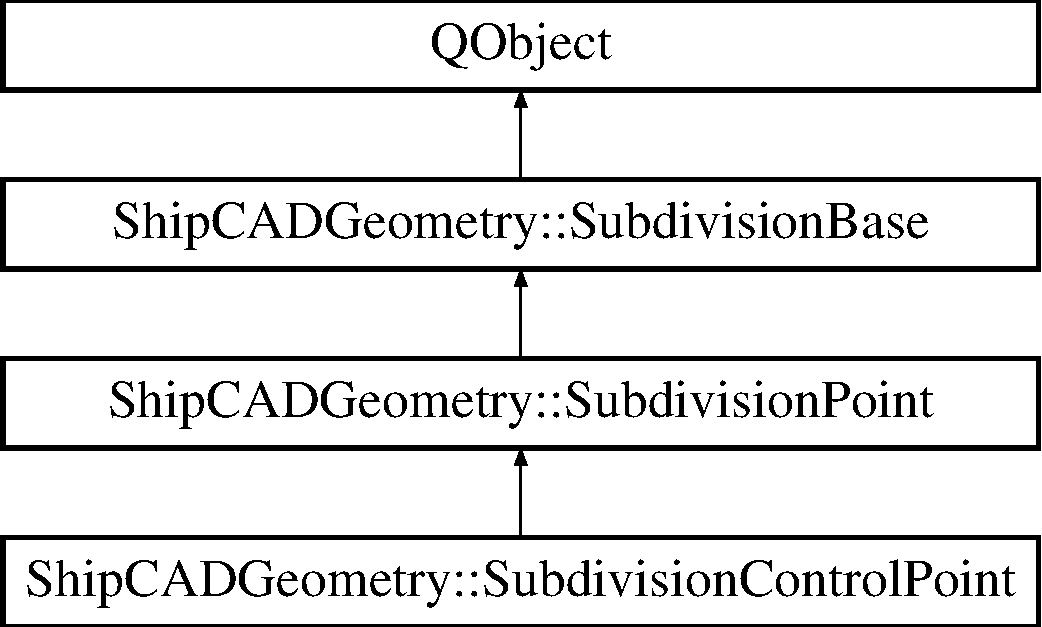
\includegraphics[height=4.000000cm]{classShipCADGeometry_1_1SubdivisionControlPoint}
\end{center}
\end{figure}
\subsection*{Public Member Functions}
\begin{DoxyCompactItemize}
\item 
\hyperlink{classShipCADGeometry_1_1SubdivisionControlPoint_a812f4e2343926ef41bc7104f0f7b1dd9}{Subdivision\-Control\-Point} (\hyperlink{classShipCADGeometry_1_1SubdivisionSurface}{Subdivision\-Surface} $\ast$owner)
\item 
virtual \hyperlink{classShipCADGeometry_1_1SubdivisionControlPoint_aed35211e2f60cd5ed1de628d732e4791}{$\sim$\-Subdivision\-Control\-Point} ()
\item 
void \hyperlink{classShipCADGeometry_1_1SubdivisionControlPoint_a3c11cf5f0a22b44cbc8674a5d82942b0}{collapse} ()
\item 
Q\-Color \hyperlink{classShipCADGeometry_1_1SubdivisionControlPoint_ad3af0386e8bb679a2037054ddbdb6a20}{get\-Color} ()
\item 
bool \hyperlink{classShipCADGeometry_1_1SubdivisionControlPoint_af446fc02c7dc2e20383e741f71f4c358}{is\-Selected} ()
\item 
bool \hyperlink{classShipCADGeometry_1_1SubdivisionControlPoint_a1d9150cdde6105519de95a94689faa51}{is\-Leak} ()
\item 
bool \hyperlink{classShipCADGeometry_1_1SubdivisionControlPoint_ad739bf09eb693c8956101d0576736239}{is\-Visible} ()
\item 
void \hyperlink{classShipCADGeometry_1_1SubdivisionControlPoint_a5642f57c7f17e78c27ad6edb0fdb7f65}{set\-Selected} (bool val)
\item 
bool \hyperlink{classShipCADGeometry_1_1SubdivisionControlPoint_aaaa65fafa27eb876db3b1d5fc646aba8}{is\-Locked} ()
\item 
void \hyperlink{classShipCADGeometry_1_1SubdivisionControlPoint_a5f2cde3c54ca44c4b4d3ded0e3bc4ded}{set\-Locked} (bool val)
\item 
virtual size\-\_\-t \hyperlink{classShipCADGeometry_1_1SubdivisionControlPoint_a13c569f0894ba6193a3abf894bc4b517}{get\-Index} ()
\item 
virtual void \hyperlink{classShipCADGeometry_1_1SubdivisionControlPoint_a54a5233e02ef34a174c24d5dcf3c6407}{set\-Coordinate} (const Q\-Vector3\-D \&val)
\item 
void \hyperlink{classShipCADGeometry_1_1SubdivisionControlPoint_a989c801ca1c836ca73f77c68d719f546}{load\-\_\-binary} (\hyperlink{classShipCADGeometry_1_1FileBuffer}{File\-Buffer} \&source)
\item 
void \hyperlink{classShipCADGeometry_1_1SubdivisionControlPoint_a7de1a32ae9e845478ec1bd5eaec17cd1}{save\-\_\-binary} (\hyperlink{classShipCADGeometry_1_1FileBuffer}{File\-Buffer} \&destination)
\item 
void \hyperlink{classShipCADGeometry_1_1SubdivisionControlPoint_a09769bfb0b63980387c23736081acdf1}{load\-From\-Stream} (size\-\_\-t \&lineno, std\-::vector$<$ Q\-String $>$ \&strings)
\item 
void \hyperlink{classShipCADGeometry_1_1SubdivisionControlPoint_a60cc866bff57473700fbea4e17adcb4d}{save\-To\-Stream} (std\-::vector$<$ Q\-String $>$ \&strings)
\item 
virtual void \hyperlink{classShipCADGeometry_1_1SubdivisionControlPoint_a4a9d6e45291c27f19f0d76c9b9d19048}{dump} (std\-::ostream \&os, const char $\ast$prefix=\char`\"{}\char`\"{}) const 
\end{DoxyCompactItemize}
\subsection*{Static Public Member Functions}
\begin{DoxyCompactItemize}
\item 
static void \hyperlink{classShipCADGeometry_1_1SubdivisionControlPoint_a761599371138b34be2c7a2cac3699e2c}{draw\-Control\-Points} (\hyperlink{classShipCADGeometry_1_1Viewport}{Viewport} \&vp, \hyperlink{classShipCADGeometry_1_1SubdivisionSurface}{Subdivision\-Surface} $\ast$surface)
\item 
static \hyperlink{classShipCADGeometry_1_1SubdivisionControlPoint}{Subdivision\-Control\-Point} $\ast$ \hyperlink{classShipCADGeometry_1_1SubdivisionControlPoint_adc189f3e5cff85ecd1a59356e0f7d63d}{construct} (\hyperlink{classShipCADGeometry_1_1SubdivisionSurface}{Subdivision\-Surface} $\ast$owner)
\end{DoxyCompactItemize}
\subsection*{Protected Member Functions}
\begin{DoxyCompactItemize}
\item 
void \hyperlink{classShipCADGeometry_1_1SubdivisionControlPoint_a01e1eff38ecb4393948db0d9883cad84}{priv\-\_\-dump} (std\-::ostream \&os, const char $\ast$prefix) const 
\end{DoxyCompactItemize}
\subsection*{Protected Attributes}
\begin{DoxyCompactItemize}
\item 
bool \hyperlink{classShipCADGeometry_1_1SubdivisionControlPoint_a65710e5c15163d01dcfdb562abb23103}{\-\_\-locked}
\end{DoxyCompactItemize}
\subsection*{Properties}
\begin{DoxyCompactItemize}
\item 
Q\-Color \hyperlink{classShipCADGeometry_1_1SubdivisionControlPoint_aecfab9d47ea8e16714ce095e3e055e55}{Color}
\item 
bool \hyperlink{classShipCADGeometry_1_1SubdivisionControlPoint_a1e192709a33919e76207ebce39c4c916}{Locked}
\item 
bool \hyperlink{classShipCADGeometry_1_1SubdivisionControlPoint_a8ae4af44e0ff44086685a9b3a362dd43}{Selected}
\item 
bool \hyperlink{classShipCADGeometry_1_1SubdivisionControlPoint_a1170db5bc9091fb18f6dfb3fd61d4413}{Visible}
\item 
bool \hyperlink{classShipCADGeometry_1_1SubdivisionControlPoint_a722a0531b6f27404b82850de2305dbea}{Is\-Leak}
\end{DoxyCompactItemize}
\subsection*{Additional Inherited Members}


\subsection{Detailed Description}


Definition at line 126 of file subdivpoint.\-h.



\subsection{Constructor \& Destructor Documentation}
\hypertarget{classShipCADGeometry_1_1SubdivisionControlPoint_a812f4e2343926ef41bc7104f0f7b1dd9}{\index{Ship\-C\-A\-D\-Geometry\-::\-Subdivision\-Control\-Point@{Ship\-C\-A\-D\-Geometry\-::\-Subdivision\-Control\-Point}!Subdivision\-Control\-Point@{Subdivision\-Control\-Point}}
\index{Subdivision\-Control\-Point@{Subdivision\-Control\-Point}!ShipCADGeometry::SubdivisionControlPoint@{Ship\-C\-A\-D\-Geometry\-::\-Subdivision\-Control\-Point}}
\subsubsection[{Subdivision\-Control\-Point}]{\setlength{\rightskip}{0pt plus 5cm}Subdivision\-Control\-Point\-::\-Subdivision\-Control\-Point (
\begin{DoxyParamCaption}
\item[{{\bf Subdivision\-Surface} $\ast$}]{owner}
\end{DoxyParamCaption}
)\hspace{0.3cm}{\ttfamily [explicit]}}}\label{classShipCADGeometry_1_1SubdivisionControlPoint_a812f4e2343926ef41bc7104f0f7b1dd9}


Definition at line 519 of file subdivpoint.\-cpp.

\hypertarget{classShipCADGeometry_1_1SubdivisionControlPoint_aed35211e2f60cd5ed1de628d732e4791}{\index{Ship\-C\-A\-D\-Geometry\-::\-Subdivision\-Control\-Point@{Ship\-C\-A\-D\-Geometry\-::\-Subdivision\-Control\-Point}!$\sim$\-Subdivision\-Control\-Point@{$\sim$\-Subdivision\-Control\-Point}}
\index{$\sim$\-Subdivision\-Control\-Point@{$\sim$\-Subdivision\-Control\-Point}!ShipCADGeometry::SubdivisionControlPoint@{Ship\-C\-A\-D\-Geometry\-::\-Subdivision\-Control\-Point}}
\subsubsection[{$\sim$\-Subdivision\-Control\-Point}]{\setlength{\rightskip}{0pt plus 5cm}Subdivision\-Control\-Point\-::$\sim$\-Subdivision\-Control\-Point (
\begin{DoxyParamCaption}
{}
\end{DoxyParamCaption}
)\hspace{0.3cm}{\ttfamily [virtual]}}}\label{classShipCADGeometry_1_1SubdivisionControlPoint_aed35211e2f60cd5ed1de628d732e4791}


Definition at line 525 of file subdivpoint.\-cpp.



\subsection{Member Function Documentation}
\hypertarget{classShipCADGeometry_1_1SubdivisionControlPoint_a3c11cf5f0a22b44cbc8674a5d82942b0}{\index{Ship\-C\-A\-D\-Geometry\-::\-Subdivision\-Control\-Point@{Ship\-C\-A\-D\-Geometry\-::\-Subdivision\-Control\-Point}!collapse@{collapse}}
\index{collapse@{collapse}!ShipCADGeometry::SubdivisionControlPoint@{Ship\-C\-A\-D\-Geometry\-::\-Subdivision\-Control\-Point}}
\subsubsection[{collapse}]{\setlength{\rightskip}{0pt plus 5cm}void Subdivision\-Control\-Point\-::collapse (
\begin{DoxyParamCaption}
{}
\end{DoxyParamCaption}
)}}\label{classShipCADGeometry_1_1SubdivisionControlPoint_a3c11cf5f0a22b44cbc8674a5d82942b0}


Definition at line 627 of file subdivpoint.\-cpp.

\hypertarget{classShipCADGeometry_1_1SubdivisionControlPoint_adc189f3e5cff85ecd1a59356e0f7d63d}{\index{Ship\-C\-A\-D\-Geometry\-::\-Subdivision\-Control\-Point@{Ship\-C\-A\-D\-Geometry\-::\-Subdivision\-Control\-Point}!construct@{construct}}
\index{construct@{construct}!ShipCADGeometry::SubdivisionControlPoint@{Ship\-C\-A\-D\-Geometry\-::\-Subdivision\-Control\-Point}}
\subsubsection[{construct}]{\setlength{\rightskip}{0pt plus 5cm}{\bf Subdivision\-Control\-Point} $\ast$ Subdivision\-Control\-Point\-::construct (
\begin{DoxyParamCaption}
\item[{{\bf Subdivision\-Surface} $\ast$}]{owner}
\end{DoxyParamCaption}
)\hspace{0.3cm}{\ttfamily [static]}}}\label{classShipCADGeometry_1_1SubdivisionControlPoint_adc189f3e5cff85ecd1a59356e0f7d63d}


Definition at line 511 of file subdivpoint.\-cpp.

\hypertarget{classShipCADGeometry_1_1SubdivisionControlPoint_a761599371138b34be2c7a2cac3699e2c}{\index{Ship\-C\-A\-D\-Geometry\-::\-Subdivision\-Control\-Point@{Ship\-C\-A\-D\-Geometry\-::\-Subdivision\-Control\-Point}!draw\-Control\-Points@{draw\-Control\-Points}}
\index{draw\-Control\-Points@{draw\-Control\-Points}!ShipCADGeometry::SubdivisionControlPoint@{Ship\-C\-A\-D\-Geometry\-::\-Subdivision\-Control\-Point}}
\subsubsection[{draw\-Control\-Points}]{\setlength{\rightskip}{0pt plus 5cm}void Subdivision\-Control\-Point\-::draw\-Control\-Points (
\begin{DoxyParamCaption}
\item[{{\bf Viewport} \&}]{vp, }
\item[{{\bf Subdivision\-Surface} $\ast$}]{surface}
\end{DoxyParamCaption}
)\hspace{0.3cm}{\ttfamily [static]}}}\label{classShipCADGeometry_1_1SubdivisionControlPoint_a761599371138b34be2c7a2cac3699e2c}


Definition at line 820 of file subdivpoint.\-cpp.

\hypertarget{classShipCADGeometry_1_1SubdivisionControlPoint_a4a9d6e45291c27f19f0d76c9b9d19048}{\index{Ship\-C\-A\-D\-Geometry\-::\-Subdivision\-Control\-Point@{Ship\-C\-A\-D\-Geometry\-::\-Subdivision\-Control\-Point}!dump@{dump}}
\index{dump@{dump}!ShipCADGeometry::SubdivisionControlPoint@{Ship\-C\-A\-D\-Geometry\-::\-Subdivision\-Control\-Point}}
\subsubsection[{dump}]{\setlength{\rightskip}{0pt plus 5cm}void Subdivision\-Control\-Point\-::dump (
\begin{DoxyParamCaption}
\item[{std\-::ostream \&}]{os, }
\item[{const char $\ast$}]{prefix = {\ttfamily \char`\"{}\char`\"{}}}
\end{DoxyParamCaption}
) const\hspace{0.3cm}{\ttfamily [virtual]}}}\label{classShipCADGeometry_1_1SubdivisionControlPoint_a4a9d6e45291c27f19f0d76c9b9d19048}


Reimplemented from \hyperlink{classShipCADGeometry_1_1SubdivisionPoint_aed72cf5e8dc67e980010d195f3a376a3}{Ship\-C\-A\-D\-Geometry\-::\-Subdivision\-Point}.



Definition at line 880 of file subdivpoint.\-cpp.

\hypertarget{classShipCADGeometry_1_1SubdivisionControlPoint_ad3af0386e8bb679a2037054ddbdb6a20}{\index{Ship\-C\-A\-D\-Geometry\-::\-Subdivision\-Control\-Point@{Ship\-C\-A\-D\-Geometry\-::\-Subdivision\-Control\-Point}!get\-Color@{get\-Color}}
\index{get\-Color@{get\-Color}!ShipCADGeometry::SubdivisionControlPoint@{Ship\-C\-A\-D\-Geometry\-::\-Subdivision\-Control\-Point}}
\subsubsection[{get\-Color}]{\setlength{\rightskip}{0pt plus 5cm}Q\-Color Subdivision\-Control\-Point\-::get\-Color (
\begin{DoxyParamCaption}
{}
\end{DoxyParamCaption}
)}}\label{classShipCADGeometry_1_1SubdivisionControlPoint_ad3af0386e8bb679a2037054ddbdb6a20}


Definition at line 532 of file subdivpoint.\-cpp.

\hypertarget{classShipCADGeometry_1_1SubdivisionControlPoint_a13c569f0894ba6193a3abf894bc4b517}{\index{Ship\-C\-A\-D\-Geometry\-::\-Subdivision\-Control\-Point@{Ship\-C\-A\-D\-Geometry\-::\-Subdivision\-Control\-Point}!get\-Index@{get\-Index}}
\index{get\-Index@{get\-Index}!ShipCADGeometry::SubdivisionControlPoint@{Ship\-C\-A\-D\-Geometry\-::\-Subdivision\-Control\-Point}}
\subsubsection[{get\-Index}]{\setlength{\rightskip}{0pt plus 5cm}size\-\_\-t Subdivision\-Control\-Point\-::get\-Index (
\begin{DoxyParamCaption}
{}
\end{DoxyParamCaption}
)\hspace{0.3cm}{\ttfamily [virtual]}}}\label{classShipCADGeometry_1_1SubdivisionControlPoint_a13c569f0894ba6193a3abf894bc4b517}


Reimplemented from \hyperlink{classShipCADGeometry_1_1SubdivisionPoint_a8406682549c10ec9e1a184132f6ed2f0}{Ship\-C\-A\-D\-Geometry\-::\-Subdivision\-Point}.



Definition at line 554 of file subdivpoint.\-cpp.

\hypertarget{classShipCADGeometry_1_1SubdivisionControlPoint_a1d9150cdde6105519de95a94689faa51}{\index{Ship\-C\-A\-D\-Geometry\-::\-Subdivision\-Control\-Point@{Ship\-C\-A\-D\-Geometry\-::\-Subdivision\-Control\-Point}!is\-Leak@{is\-Leak}}
\index{is\-Leak@{is\-Leak}!ShipCADGeometry::SubdivisionControlPoint@{Ship\-C\-A\-D\-Geometry\-::\-Subdivision\-Control\-Point}}
\subsubsection[{is\-Leak}]{\setlength{\rightskip}{0pt plus 5cm}bool Subdivision\-Control\-Point\-::is\-Leak (
\begin{DoxyParamCaption}
{}
\end{DoxyParamCaption}
)}}\label{classShipCADGeometry_1_1SubdivisionControlPoint_a1d9150cdde6105519de95a94689faa51}


Definition at line 598 of file subdivpoint.\-cpp.

\hypertarget{classShipCADGeometry_1_1SubdivisionControlPoint_aaaa65fafa27eb876db3b1d5fc646aba8}{\index{Ship\-C\-A\-D\-Geometry\-::\-Subdivision\-Control\-Point@{Ship\-C\-A\-D\-Geometry\-::\-Subdivision\-Control\-Point}!is\-Locked@{is\-Locked}}
\index{is\-Locked@{is\-Locked}!ShipCADGeometry::SubdivisionControlPoint@{Ship\-C\-A\-D\-Geometry\-::\-Subdivision\-Control\-Point}}
\subsubsection[{is\-Locked}]{\setlength{\rightskip}{0pt plus 5cm}bool Ship\-C\-A\-D\-Geometry\-::\-Subdivision\-Control\-Point\-::is\-Locked (
\begin{DoxyParamCaption}
{}
\end{DoxyParamCaption}
)\hspace{0.3cm}{\ttfamily [inline]}}}\label{classShipCADGeometry_1_1SubdivisionControlPoint_aaaa65fafa27eb876db3b1d5fc646aba8}


Definition at line 148 of file subdivpoint.\-h.

\hypertarget{classShipCADGeometry_1_1SubdivisionControlPoint_af446fc02c7dc2e20383e741f71f4c358}{\index{Ship\-C\-A\-D\-Geometry\-::\-Subdivision\-Control\-Point@{Ship\-C\-A\-D\-Geometry\-::\-Subdivision\-Control\-Point}!is\-Selected@{is\-Selected}}
\index{is\-Selected@{is\-Selected}!ShipCADGeometry::SubdivisionControlPoint@{Ship\-C\-A\-D\-Geometry\-::\-Subdivision\-Control\-Point}}
\subsubsection[{is\-Selected}]{\setlength{\rightskip}{0pt plus 5cm}bool Subdivision\-Control\-Point\-::is\-Selected (
\begin{DoxyParamCaption}
{}
\end{DoxyParamCaption}
)}}\label{classShipCADGeometry_1_1SubdivisionControlPoint_af446fc02c7dc2e20383e741f71f4c358}


Definition at line 559 of file subdivpoint.\-cpp.

\hypertarget{classShipCADGeometry_1_1SubdivisionControlPoint_ad739bf09eb693c8956101d0576736239}{\index{Ship\-C\-A\-D\-Geometry\-::\-Subdivision\-Control\-Point@{Ship\-C\-A\-D\-Geometry\-::\-Subdivision\-Control\-Point}!is\-Visible@{is\-Visible}}
\index{is\-Visible@{is\-Visible}!ShipCADGeometry::SubdivisionControlPoint@{Ship\-C\-A\-D\-Geometry\-::\-Subdivision\-Control\-Point}}
\subsubsection[{is\-Visible}]{\setlength{\rightskip}{0pt plus 5cm}bool Subdivision\-Control\-Point\-::is\-Visible (
\begin{DoxyParamCaption}
{}
\end{DoxyParamCaption}
)}}\label{classShipCADGeometry_1_1SubdivisionControlPoint_ad739bf09eb693c8956101d0576736239}


Definition at line 564 of file subdivpoint.\-cpp.

\hypertarget{classShipCADGeometry_1_1SubdivisionControlPoint_a989c801ca1c836ca73f77c68d719f546}{\index{Ship\-C\-A\-D\-Geometry\-::\-Subdivision\-Control\-Point@{Ship\-C\-A\-D\-Geometry\-::\-Subdivision\-Control\-Point}!load\-\_\-binary@{load\-\_\-binary}}
\index{load\-\_\-binary@{load\-\_\-binary}!ShipCADGeometry::SubdivisionControlPoint@{Ship\-C\-A\-D\-Geometry\-::\-Subdivision\-Control\-Point}}
\subsubsection[{load\-\_\-binary}]{\setlength{\rightskip}{0pt plus 5cm}void Subdivision\-Control\-Point\-::load\-\_\-binary (
\begin{DoxyParamCaption}
\item[{{\bf File\-Buffer} \&}]{source}
\end{DoxyParamCaption}
)}}\label{classShipCADGeometry_1_1SubdivisionControlPoint_a989c801ca1c836ca73f77c68d719f546}


Definition at line 764 of file subdivpoint.\-cpp.

\hypertarget{classShipCADGeometry_1_1SubdivisionControlPoint_a09769bfb0b63980387c23736081acdf1}{\index{Ship\-C\-A\-D\-Geometry\-::\-Subdivision\-Control\-Point@{Ship\-C\-A\-D\-Geometry\-::\-Subdivision\-Control\-Point}!load\-From\-Stream@{load\-From\-Stream}}
\index{load\-From\-Stream@{load\-From\-Stream}!ShipCADGeometry::SubdivisionControlPoint@{Ship\-C\-A\-D\-Geometry\-::\-Subdivision\-Control\-Point}}
\subsubsection[{load\-From\-Stream}]{\setlength{\rightskip}{0pt plus 5cm}void Subdivision\-Control\-Point\-::load\-From\-Stream (
\begin{DoxyParamCaption}
\item[{size\-\_\-t \&}]{lineno, }
\item[{std\-::vector$<$ Q\-String $>$ \&}]{strings}
\end{DoxyParamCaption}
)}}\label{classShipCADGeometry_1_1SubdivisionControlPoint_a09769bfb0b63980387c23736081acdf1}


Definition at line 778 of file subdivpoint.\-cpp.

\hypertarget{classShipCADGeometry_1_1SubdivisionControlPoint_a01e1eff38ecb4393948db0d9883cad84}{\index{Ship\-C\-A\-D\-Geometry\-::\-Subdivision\-Control\-Point@{Ship\-C\-A\-D\-Geometry\-::\-Subdivision\-Control\-Point}!priv\-\_\-dump@{priv\-\_\-dump}}
\index{priv\-\_\-dump@{priv\-\_\-dump}!ShipCADGeometry::SubdivisionControlPoint@{Ship\-C\-A\-D\-Geometry\-::\-Subdivision\-Control\-Point}}
\subsubsection[{priv\-\_\-dump}]{\setlength{\rightskip}{0pt plus 5cm}void Subdivision\-Control\-Point\-::priv\-\_\-dump (
\begin{DoxyParamCaption}
\item[{std\-::ostream \&}]{os, }
\item[{const char $\ast$}]{prefix}
\end{DoxyParamCaption}
) const\hspace{0.3cm}{\ttfamily [protected]}}}\label{classShipCADGeometry_1_1SubdivisionControlPoint_a01e1eff38ecb4393948db0d9883cad84}


Definition at line 888 of file subdivpoint.\-cpp.

\hypertarget{classShipCADGeometry_1_1SubdivisionControlPoint_a7de1a32ae9e845478ec1bd5eaec17cd1}{\index{Ship\-C\-A\-D\-Geometry\-::\-Subdivision\-Control\-Point@{Ship\-C\-A\-D\-Geometry\-::\-Subdivision\-Control\-Point}!save\-\_\-binary@{save\-\_\-binary}}
\index{save\-\_\-binary@{save\-\_\-binary}!ShipCADGeometry::SubdivisionControlPoint@{Ship\-C\-A\-D\-Geometry\-::\-Subdivision\-Control\-Point}}
\subsubsection[{save\-\_\-binary}]{\setlength{\rightskip}{0pt plus 5cm}void Subdivision\-Control\-Point\-::save\-\_\-binary (
\begin{DoxyParamCaption}
\item[{{\bf File\-Buffer} \&}]{destination}
\end{DoxyParamCaption}
)}}\label{classShipCADGeometry_1_1SubdivisionControlPoint_a7de1a32ae9e845478ec1bd5eaec17cd1}


Definition at line 811 of file subdivpoint.\-cpp.

\hypertarget{classShipCADGeometry_1_1SubdivisionControlPoint_a60cc866bff57473700fbea4e17adcb4d}{\index{Ship\-C\-A\-D\-Geometry\-::\-Subdivision\-Control\-Point@{Ship\-C\-A\-D\-Geometry\-::\-Subdivision\-Control\-Point}!save\-To\-Stream@{save\-To\-Stream}}
\index{save\-To\-Stream@{save\-To\-Stream}!ShipCADGeometry::SubdivisionControlPoint@{Ship\-C\-A\-D\-Geometry\-::\-Subdivision\-Control\-Point}}
\subsubsection[{save\-To\-Stream}]{\setlength{\rightskip}{0pt plus 5cm}void Subdivision\-Control\-Point\-::save\-To\-Stream (
\begin{DoxyParamCaption}
\item[{std\-::vector$<$ Q\-String $>$ \&}]{strings}
\end{DoxyParamCaption}
)}}\label{classShipCADGeometry_1_1SubdivisionControlPoint_a60cc866bff57473700fbea4e17adcb4d}


Definition at line 800 of file subdivpoint.\-cpp.

\hypertarget{classShipCADGeometry_1_1SubdivisionControlPoint_a54a5233e02ef34a174c24d5dcf3c6407}{\index{Ship\-C\-A\-D\-Geometry\-::\-Subdivision\-Control\-Point@{Ship\-C\-A\-D\-Geometry\-::\-Subdivision\-Control\-Point}!set\-Coordinate@{set\-Coordinate}}
\index{set\-Coordinate@{set\-Coordinate}!ShipCADGeometry::SubdivisionControlPoint@{Ship\-C\-A\-D\-Geometry\-::\-Subdivision\-Control\-Point}}
\subsubsection[{set\-Coordinate}]{\setlength{\rightskip}{0pt plus 5cm}void Subdivision\-Control\-Point\-::set\-Coordinate (
\begin{DoxyParamCaption}
\item[{const Q\-Vector3\-D \&}]{val}
\end{DoxyParamCaption}
)\hspace{0.3cm}{\ttfamily [virtual]}}}\label{classShipCADGeometry_1_1SubdivisionControlPoint_a54a5233e02ef34a174c24d5dcf3c6407}


Reimplemented from \hyperlink{classShipCADGeometry_1_1SubdivisionPoint_a98ab99a0ccc4709a40e05b36147c0f55}{Ship\-C\-A\-D\-Geometry\-::\-Subdivision\-Point}.



Definition at line 621 of file subdivpoint.\-cpp.

\hypertarget{classShipCADGeometry_1_1SubdivisionControlPoint_a5f2cde3c54ca44c4b4d3ded0e3bc4ded}{\index{Ship\-C\-A\-D\-Geometry\-::\-Subdivision\-Control\-Point@{Ship\-C\-A\-D\-Geometry\-::\-Subdivision\-Control\-Point}!set\-Locked@{set\-Locked}}
\index{set\-Locked@{set\-Locked}!ShipCADGeometry::SubdivisionControlPoint@{Ship\-C\-A\-D\-Geometry\-::\-Subdivision\-Control\-Point}}
\subsubsection[{set\-Locked}]{\setlength{\rightskip}{0pt plus 5cm}void Subdivision\-Control\-Point\-::set\-Locked (
\begin{DoxyParamCaption}
\item[{bool}]{val}
\end{DoxyParamCaption}
)}}\label{classShipCADGeometry_1_1SubdivisionControlPoint_a5f2cde3c54ca44c4b4d3ded0e3bc4ded}


Definition at line 615 of file subdivpoint.\-cpp.

\hypertarget{classShipCADGeometry_1_1SubdivisionControlPoint_a5642f57c7f17e78c27ad6edb0fdb7f65}{\index{Ship\-C\-A\-D\-Geometry\-::\-Subdivision\-Control\-Point@{Ship\-C\-A\-D\-Geometry\-::\-Subdivision\-Control\-Point}!set\-Selected@{set\-Selected}}
\index{set\-Selected@{set\-Selected}!ShipCADGeometry::SubdivisionControlPoint@{Ship\-C\-A\-D\-Geometry\-::\-Subdivision\-Control\-Point}}
\subsubsection[{set\-Selected}]{\setlength{\rightskip}{0pt plus 5cm}void Subdivision\-Control\-Point\-::set\-Selected (
\begin{DoxyParamCaption}
\item[{bool}]{val}
\end{DoxyParamCaption}
)}}\label{classShipCADGeometry_1_1SubdivisionControlPoint_a5642f57c7f17e78c27ad6edb0fdb7f65}


Definition at line 603 of file subdivpoint.\-cpp.



\subsection{Member Data Documentation}
\hypertarget{classShipCADGeometry_1_1SubdivisionControlPoint_a65710e5c15163d01dcfdb562abb23103}{\index{Ship\-C\-A\-D\-Geometry\-::\-Subdivision\-Control\-Point@{Ship\-C\-A\-D\-Geometry\-::\-Subdivision\-Control\-Point}!\-\_\-locked@{\-\_\-locked}}
\index{\-\_\-locked@{\-\_\-locked}!ShipCADGeometry::SubdivisionControlPoint@{Ship\-C\-A\-D\-Geometry\-::\-Subdivision\-Control\-Point}}
\subsubsection[{\-\_\-locked}]{\setlength{\rightskip}{0pt plus 5cm}bool Ship\-C\-A\-D\-Geometry\-::\-Subdivision\-Control\-Point\-::\-\_\-locked\hspace{0.3cm}{\ttfamily [protected]}}}\label{classShipCADGeometry_1_1SubdivisionControlPoint_a65710e5c15163d01dcfdb562abb23103}


Definition at line 174 of file subdivpoint.\-h.



\subsection{Property Documentation}
\hypertarget{classShipCADGeometry_1_1SubdivisionControlPoint_aecfab9d47ea8e16714ce095e3e055e55}{\index{Ship\-C\-A\-D\-Geometry\-::\-Subdivision\-Control\-Point@{Ship\-C\-A\-D\-Geometry\-::\-Subdivision\-Control\-Point}!Color@{Color}}
\index{Color@{Color}!ShipCADGeometry::SubdivisionControlPoint@{Ship\-C\-A\-D\-Geometry\-::\-Subdivision\-Control\-Point}}
\subsubsection[{Color}]{\setlength{\rightskip}{0pt plus 5cm}Q\-Color Ship\-C\-A\-D\-Geometry\-::\-Subdivision\-Control\-Point\-::\-Color\hspace{0.3cm}{\ttfamily [read]}}}\label{classShipCADGeometry_1_1SubdivisionControlPoint_aecfab9d47ea8e16714ce095e3e055e55}


Definition at line 129 of file subdivpoint.\-h.

\hypertarget{classShipCADGeometry_1_1SubdivisionControlPoint_a722a0531b6f27404b82850de2305dbea}{\index{Ship\-C\-A\-D\-Geometry\-::\-Subdivision\-Control\-Point@{Ship\-C\-A\-D\-Geometry\-::\-Subdivision\-Control\-Point}!Is\-Leak@{Is\-Leak}}
\index{Is\-Leak@{Is\-Leak}!ShipCADGeometry::SubdivisionControlPoint@{Ship\-C\-A\-D\-Geometry\-::\-Subdivision\-Control\-Point}}
\subsubsection[{Is\-Leak}]{\setlength{\rightskip}{0pt plus 5cm}bool Ship\-C\-A\-D\-Geometry\-::\-Subdivision\-Control\-Point\-::\-Is\-Leak\hspace{0.3cm}{\ttfamily [read]}}}\label{classShipCADGeometry_1_1SubdivisionControlPoint_a722a0531b6f27404b82850de2305dbea}


Definition at line 133 of file subdivpoint.\-h.

\hypertarget{classShipCADGeometry_1_1SubdivisionControlPoint_a1e192709a33919e76207ebce39c4c916}{\index{Ship\-C\-A\-D\-Geometry\-::\-Subdivision\-Control\-Point@{Ship\-C\-A\-D\-Geometry\-::\-Subdivision\-Control\-Point}!Locked@{Locked}}
\index{Locked@{Locked}!ShipCADGeometry::SubdivisionControlPoint@{Ship\-C\-A\-D\-Geometry\-::\-Subdivision\-Control\-Point}}
\subsubsection[{Locked}]{\setlength{\rightskip}{0pt plus 5cm}bool Ship\-C\-A\-D\-Geometry\-::\-Subdivision\-Control\-Point\-::\-Locked\hspace{0.3cm}{\ttfamily [read]}, {\ttfamily [write]}}}\label{classShipCADGeometry_1_1SubdivisionControlPoint_a1e192709a33919e76207ebce39c4c916}


Definition at line 130 of file subdivpoint.\-h.

\hypertarget{classShipCADGeometry_1_1SubdivisionControlPoint_a8ae4af44e0ff44086685a9b3a362dd43}{\index{Ship\-C\-A\-D\-Geometry\-::\-Subdivision\-Control\-Point@{Ship\-C\-A\-D\-Geometry\-::\-Subdivision\-Control\-Point}!Selected@{Selected}}
\index{Selected@{Selected}!ShipCADGeometry::SubdivisionControlPoint@{Ship\-C\-A\-D\-Geometry\-::\-Subdivision\-Control\-Point}}
\subsubsection[{Selected}]{\setlength{\rightskip}{0pt plus 5cm}bool Ship\-C\-A\-D\-Geometry\-::\-Subdivision\-Control\-Point\-::\-Selected\hspace{0.3cm}{\ttfamily [read]}, {\ttfamily [write]}}}\label{classShipCADGeometry_1_1SubdivisionControlPoint_a8ae4af44e0ff44086685a9b3a362dd43}


Definition at line 131 of file subdivpoint.\-h.

\hypertarget{classShipCADGeometry_1_1SubdivisionControlPoint_a1170db5bc9091fb18f6dfb3fd61d4413}{\index{Ship\-C\-A\-D\-Geometry\-::\-Subdivision\-Control\-Point@{Ship\-C\-A\-D\-Geometry\-::\-Subdivision\-Control\-Point}!Visible@{Visible}}
\index{Visible@{Visible}!ShipCADGeometry::SubdivisionControlPoint@{Ship\-C\-A\-D\-Geometry\-::\-Subdivision\-Control\-Point}}
\subsubsection[{Visible}]{\setlength{\rightskip}{0pt plus 5cm}bool Ship\-C\-A\-D\-Geometry\-::\-Subdivision\-Control\-Point\-::\-Visible\hspace{0.3cm}{\ttfamily [read]}}}\label{classShipCADGeometry_1_1SubdivisionControlPoint_a1170db5bc9091fb18f6dfb3fd61d4413}


Definition at line 132 of file subdivpoint.\-h.



The documentation for this class was generated from the following files\-:\begin{DoxyCompactItemize}
\item 
Ship\-C\-A\-Dlib/\hyperlink{subdivpoint_8h}{subdivpoint.\-h}\item 
Ship\-C\-A\-Dlib/\hyperlink{subdivpoint_8cpp}{subdivpoint.\-cpp}\end{DoxyCompactItemize}

\hypertarget{classShipCADGeometry_1_1SubdivisionEdge}{\section{Ship\-C\-A\-D\-Geometry\-:\-:Subdivision\-Edge Class Reference}
\label{classShipCADGeometry_1_1SubdivisionEdge}\index{Ship\-C\-A\-D\-Geometry\-::\-Subdivision\-Edge@{Ship\-C\-A\-D\-Geometry\-::\-Subdivision\-Edge}}
}


{\ttfamily \#include $<$subdivedge.\-h$>$}

Inheritance diagram for Ship\-C\-A\-D\-Geometry\-:\-:Subdivision\-Edge\-:\begin{figure}[H]
\begin{center}
\leavevmode
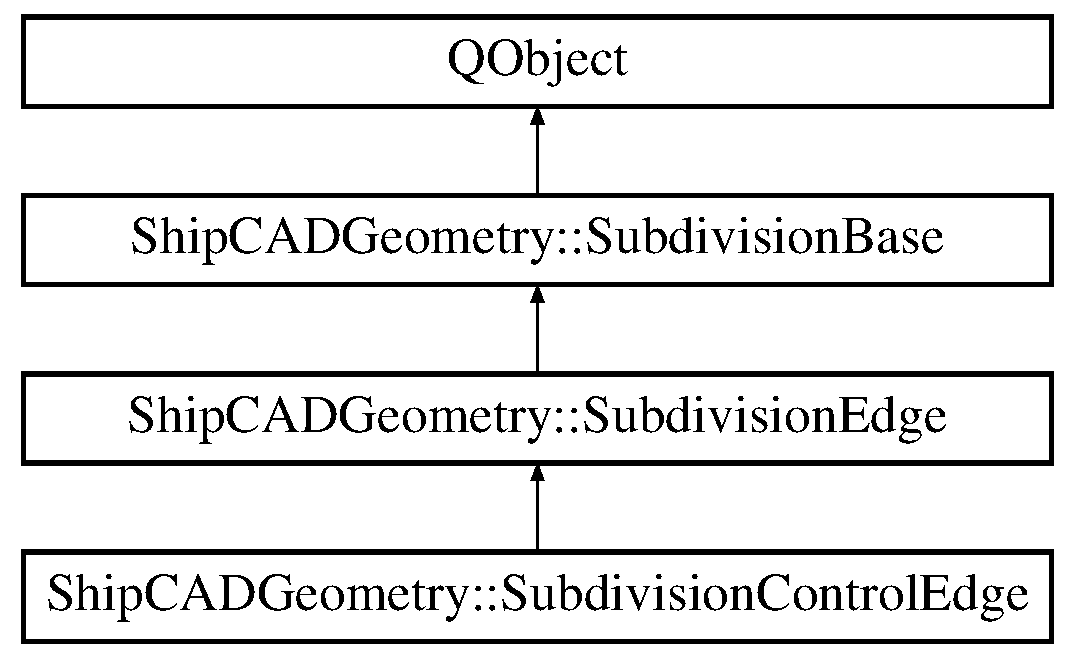
\includegraphics[height=4.000000cm]{classShipCADGeometry_1_1SubdivisionEdge}
\end{center}
\end{figure}
\subsection*{Public Member Functions}
\begin{DoxyCompactItemize}
\item 
\hyperlink{classShipCADGeometry_1_1SubdivisionEdge_ab08271ed7f5d371f0495d8a7d2c96dae}{Subdivision\-Edge} (\hyperlink{classShipCADGeometry_1_1SubdivisionSurface}{Subdivision\-Surface} $\ast$owner)
\item 
virtual \hyperlink{classShipCADGeometry_1_1SubdivisionEdge_ac787ad1a0228f91038de9518ad217364}{$\sim$\-Subdivision\-Edge} ()
\item 
virtual void \hyperlink{classShipCADGeometry_1_1SubdivisionEdge_a08358ac65c2d710855b8b93c64ce9d02}{clear} ()
\begin{DoxyCompactList}\small\item\em reset this element to default values \end{DoxyCompactList}\item 
virtual void \hyperlink{classShipCADGeometry_1_1SubdivisionEdge_a26deda12672fa679b49b28f2371e728b}{draw} (bool draw\-\_\-mirror, \hyperlink{classShipCADGeometry_1_1Viewport}{Viewport} \&vp, \hyperlink{classShipCADGeometry_1_1LineShader}{Line\-Shader} $\ast$lineshader, const Q\-Color \&edge\-Color)
\item 
void \hyperlink{classShipCADGeometry_1_1SubdivisionEdge_a1b2e2b1d7e051d42250c0ad1f5eaa560}{add\-Face} (\hyperlink{classShipCADGeometry_1_1SubdivisionFace}{Subdivision\-Face} $\ast$face)
\item 
void \hyperlink{classShipCADGeometry_1_1SubdivisionEdge_ab91ca7bbcd013cc01e90b077ea1aae9b}{assign} (\hyperlink{classShipCADGeometry_1_1SubdivisionEdge}{Subdivision\-Edge} $\ast$edge)
\item 
\hyperlink{classShipCADGeometry_1_1SubdivisionPoint}{Subdivision\-Point} $\ast$ \hyperlink{classShipCADGeometry_1_1SubdivisionEdge_aa1bce1c13f4911839205e812cfd0f683}{calculate\-Edge\-Point} ()
\item 
void \hyperlink{classShipCADGeometry_1_1SubdivisionEdge_a1f4b70ab6d0c4dfec07a2d4348bc9a3e}{delete\-Face} (\hyperlink{classShipCADGeometry_1_1SubdivisionFace}{Subdivision\-Face} $\ast$face)
\item 
void \hyperlink{classShipCADGeometry_1_1SubdivisionEdge_ad19ddea08367fa2307e131132e36c008}{swap\-Data} ()
\item 
\hyperlink{classShipCADGeometry_1_1SubdivisionPoint}{Subdivision\-Point} $\ast$ \hyperlink{classShipCADGeometry_1_1SubdivisionEdge_a0d8b0bc79b1f8d19f2c4798251aeff31}{start\-Point} ()
\item 
\hyperlink{classShipCADGeometry_1_1SubdivisionPoint}{Subdivision\-Point} $\ast$ \hyperlink{classShipCADGeometry_1_1SubdivisionEdge_a6d98a4d163b1beae788038f36b5ee2fe}{end\-Point} ()
\item 
virtual bool \hyperlink{classShipCADGeometry_1_1SubdivisionEdge_ad95a3ec8ba66deb74cbfd3d36428fc34}{is\-Boundary\-Edge} ()
\item 
bool \hyperlink{classShipCADGeometry_1_1SubdivisionEdge_ae47df0c89e604d2185c12ef1be43e535}{is\-Control\-Edge} ()
\item 
void \hyperlink{classShipCADGeometry_1_1SubdivisionEdge_aef8475bab828f5e100dd12699f0aad9b}{set\-Control\-Edge} (bool val)
\item 
size\-\_\-t \hyperlink{classShipCADGeometry_1_1SubdivisionEdge_a9120bf0ef10c838cd69e402eecd8c896}{number\-Of\-Faces} ()
\item 
bool \hyperlink{classShipCADGeometry_1_1SubdivisionEdge_a26be9f91b5fae2c62b99ea501e4a6015}{is\-Crease} ()
\item 
void \hyperlink{classShipCADGeometry_1_1SubdivisionEdge_ad0313b8844a81c5802533376a09fce99}{set\-Crease} (bool val)
\item 
\hyperlink{classShipCADGeometry_1_1SubdivisionControlCurve}{Subdivision\-Control\-Curve} $\ast$ \hyperlink{classShipCADGeometry_1_1SubdivisionEdge_afb80c9ae06d2bb9bb596e2eac6efa993}{get\-Curve} ()
\item 
void \hyperlink{classShipCADGeometry_1_1SubdivisionEdge_a6412679e0438dac8545200df59480783}{set\-Curve} (\hyperlink{classShipCADGeometry_1_1SubdivisionControlCurve}{Subdivision\-Control\-Curve} $\ast$curve)
\item 
size\-\_\-t \hyperlink{classShipCADGeometry_1_1SubdivisionEdge_a4be990243bb29ead43c76171197130d5}{get\-Index} ()
\item 
\hyperlink{classShipCADGeometry_1_1SubdivisionFace}{Subdivision\-Face} $\ast$ \hyperlink{classShipCADGeometry_1_1SubdivisionEdge_a55dc9daab165567ed40e37f9e01ee766}{get\-Face} (size\-\_\-t index)
\item 
bool \hyperlink{classShipCADGeometry_1_1SubdivisionEdge_a286bc4d7959703a153945e3bcb9c9ad3}{has\-Face} (\hyperlink{classShipCADGeometry_1_1SubdivisionFace}{Subdivision\-Face} $\ast$face)
\item 
\hyperlink{classShipCADGeometry_1_1SubdivisionEdge}{Subdivision\-Edge} $\ast$ \hyperlink{classShipCADGeometry_1_1SubdivisionEdge_a7c1fe2cad6e7b8a0e532768b4a395137}{get\-Previous\-Edge} ()
\item 
\hyperlink{classShipCADGeometry_1_1SubdivisionEdge}{Subdivision\-Edge} $\ast$ \hyperlink{classShipCADGeometry_1_1SubdivisionEdge_aebb50514ff119a1484f7c7505a527a2b}{get\-Next\-Edge} ()
\item 
void \hyperlink{classShipCADGeometry_1_1SubdivisionEdge_affa2f4fab16979100d12f1823b26aa9c}{set\-Points} (\hyperlink{classShipCADGeometry_1_1SubdivisionPoint}{Subdivision\-Point} $\ast$p1, \hyperlink{classShipCADGeometry_1_1SubdivisionPoint}{Subdivision\-Point} $\ast$p2)
\item 
virtual void \hyperlink{classShipCADGeometry_1_1SubdivisionEdge_a14cc58877644ebd7b7ebffbdf8ef87f7}{dump} (std\-::ostream \&os, const char $\ast$prefix=\char`\"{}\char`\"{}) const 
\begin{DoxyCompactList}\small\item\em print out the element to a stream \end{DoxyCompactList}\end{DoxyCompactItemize}
\subsection*{Static Public Member Functions}
\begin{DoxyCompactItemize}
\item 
static \hyperlink{classShipCADGeometry_1_1SubdivisionEdge}{Subdivision\-Edge} $\ast$ \hyperlink{classShipCADGeometry_1_1SubdivisionEdge_ac2e94f4689d724a1d5b75c7f2619c37d}{construct} (\hyperlink{classShipCADGeometry_1_1SubdivisionSurface}{Subdivision\-Surface} $\ast$owner)
\end{DoxyCompactItemize}
\subsection*{Protected Member Functions}
\begin{DoxyCompactItemize}
\item 
void \hyperlink{classShipCADGeometry_1_1SubdivisionEdge_a8b33f4ae9edbd8ac4a386d9f5f5c1131}{priv\-\_\-dump} (std\-::ostream \&os, const char $\ast$prefix) const 
\end{DoxyCompactItemize}
\subsection*{Protected Attributes}
\begin{DoxyCompactItemize}
\item 
\hyperlink{classShipCADGeometry_1_1SubdivisionPoint}{Subdivision\-Point} $\ast$ \hyperlink{classShipCADGeometry_1_1SubdivisionEdge_a1df486b149723fe19190b178897f9a27}{\-\_\-points} \mbox{[}2\mbox{]}
\item 
std\-::vector$<$ \hyperlink{classShipCADGeometry_1_1SubdivisionFace}{Subdivision\-Face} $\ast$ $>$ \hyperlink{classShipCADGeometry_1_1SubdivisionEdge_af74c555a9f1e520c8a7092819182c565}{\-\_\-faces}
\item 
bool \hyperlink{classShipCADGeometry_1_1SubdivisionEdge_ae098b2abe43d484178e743a4e0ee2dd1}{\-\_\-crease}
\item 
bool \hyperlink{classShipCADGeometry_1_1SubdivisionEdge_a0253d92464fa44ece75199bafc2ab604}{\-\_\-control\-\_\-edge}
\item 
\hyperlink{classShipCADGeometry_1_1SubdivisionControlCurve}{Subdivision\-Control\-Curve} $\ast$ \hyperlink{classShipCADGeometry_1_1SubdivisionEdge_ae3d4de49a5c6b332d52a6c4e98704183}{\-\_\-curve}
\end{DoxyCompactItemize}
\subsection*{Properties}
\begin{DoxyCompactItemize}
\item 
\hyperlink{classShipCADGeometry_1_1SubdivisionPoint}{Subdivision\-Point} \hyperlink{classShipCADGeometry_1_1SubdivisionEdge_add30db0d6a7aac1c8f081012f3cccf03}{Start\-Point}
\item 
\hyperlink{classShipCADGeometry_1_1SubdivisionPoint}{Subdivision\-Point} \hyperlink{classShipCADGeometry_1_1SubdivisionEdge_aaec4f19ba8274a3b501a06fedb0658cb}{End\-Point}
\item 
bool \hyperlink{classShipCADGeometry_1_1SubdivisionEdge_ab36f0260a63d4ca62c45feddf96f8505}{Crease}
\item 
size\-\_\-t \hyperlink{classShipCADGeometry_1_1SubdivisionEdge_a5d959fb5043fcad1c24e603b50e9fa95}{Index}
\item 
\hyperlink{classShipCADGeometry_1_1SubdivisionControlCurve}{Subdivision\-Control\-Curve} \hyperlink{classShipCADGeometry_1_1SubdivisionEdge_abdc110088d3e486395a31dd7c7328dd4}{Curve}
\item 
bool \hyperlink{classShipCADGeometry_1_1SubdivisionEdge_a2b11b00bcc223691e6e00c4b8db272b6}{Control\-Edge}
\end{DoxyCompactItemize}


\subsection{Detailed Description}


Definition at line 54 of file subdivedge.\-h.



\subsection{Constructor \& Destructor Documentation}
\hypertarget{classShipCADGeometry_1_1SubdivisionEdge_ab08271ed7f5d371f0495d8a7d2c96dae}{\index{Ship\-C\-A\-D\-Geometry\-::\-Subdivision\-Edge@{Ship\-C\-A\-D\-Geometry\-::\-Subdivision\-Edge}!Subdivision\-Edge@{Subdivision\-Edge}}
\index{Subdivision\-Edge@{Subdivision\-Edge}!ShipCADGeometry::SubdivisionEdge@{Ship\-C\-A\-D\-Geometry\-::\-Subdivision\-Edge}}
\subsubsection[{Subdivision\-Edge}]{\setlength{\rightskip}{0pt plus 5cm}Subdivision\-Edge\-::\-Subdivision\-Edge (
\begin{DoxyParamCaption}
\item[{{\bf Subdivision\-Surface} $\ast$}]{owner}
\end{DoxyParamCaption}
)\hspace{0.3cm}{\ttfamily [explicit]}}}\label{classShipCADGeometry_1_1SubdivisionEdge_ab08271ed7f5d371f0495d8a7d2c96dae}


Definition at line 62 of file subdivedge.\-cpp.

\hypertarget{classShipCADGeometry_1_1SubdivisionEdge_ac787ad1a0228f91038de9518ad217364}{\index{Ship\-C\-A\-D\-Geometry\-::\-Subdivision\-Edge@{Ship\-C\-A\-D\-Geometry\-::\-Subdivision\-Edge}!$\sim$\-Subdivision\-Edge@{$\sim$\-Subdivision\-Edge}}
\index{$\sim$\-Subdivision\-Edge@{$\sim$\-Subdivision\-Edge}!ShipCADGeometry::SubdivisionEdge@{Ship\-C\-A\-D\-Geometry\-::\-Subdivision\-Edge}}
\subsubsection[{$\sim$\-Subdivision\-Edge}]{\setlength{\rightskip}{0pt plus 5cm}Subdivision\-Edge\-::$\sim$\-Subdivision\-Edge (
\begin{DoxyParamCaption}
{}
\end{DoxyParamCaption}
)\hspace{0.3cm}{\ttfamily [virtual]}}}\label{classShipCADGeometry_1_1SubdivisionEdge_ac787ad1a0228f91038de9518ad217364}


Definition at line 68 of file subdivedge.\-cpp.



\subsection{Member Function Documentation}
\hypertarget{classShipCADGeometry_1_1SubdivisionEdge_a1b2e2b1d7e051d42250c0ad1f5eaa560}{\index{Ship\-C\-A\-D\-Geometry\-::\-Subdivision\-Edge@{Ship\-C\-A\-D\-Geometry\-::\-Subdivision\-Edge}!add\-Face@{add\-Face}}
\index{add\-Face@{add\-Face}!ShipCADGeometry::SubdivisionEdge@{Ship\-C\-A\-D\-Geometry\-::\-Subdivision\-Edge}}
\subsubsection[{add\-Face}]{\setlength{\rightskip}{0pt plus 5cm}void Subdivision\-Edge\-::add\-Face (
\begin{DoxyParamCaption}
\item[{{\bf Subdivision\-Face} $\ast$}]{face}
\end{DoxyParamCaption}
)}}\label{classShipCADGeometry_1_1SubdivisionEdge_a1b2e2b1d7e051d42250c0ad1f5eaa560}


Definition at line 227 of file subdivedge.\-cpp.

\hypertarget{classShipCADGeometry_1_1SubdivisionEdge_ab91ca7bbcd013cc01e90b077ea1aae9b}{\index{Ship\-C\-A\-D\-Geometry\-::\-Subdivision\-Edge@{Ship\-C\-A\-D\-Geometry\-::\-Subdivision\-Edge}!assign@{assign}}
\index{assign@{assign}!ShipCADGeometry::SubdivisionEdge@{Ship\-C\-A\-D\-Geometry\-::\-Subdivision\-Edge}}
\subsubsection[{assign}]{\setlength{\rightskip}{0pt plus 5cm}void Ship\-C\-A\-D\-Geometry\-::\-Subdivision\-Edge\-::assign (
\begin{DoxyParamCaption}
\item[{{\bf Subdivision\-Edge} $\ast$}]{edge}
\end{DoxyParamCaption}
)}}\label{classShipCADGeometry_1_1SubdivisionEdge_ab91ca7bbcd013cc01e90b077ea1aae9b}
\hypertarget{classShipCADGeometry_1_1SubdivisionEdge_aa1bce1c13f4911839205e812cfd0f683}{\index{Ship\-C\-A\-D\-Geometry\-::\-Subdivision\-Edge@{Ship\-C\-A\-D\-Geometry\-::\-Subdivision\-Edge}!calculate\-Edge\-Point@{calculate\-Edge\-Point}}
\index{calculate\-Edge\-Point@{calculate\-Edge\-Point}!ShipCADGeometry::SubdivisionEdge@{Ship\-C\-A\-D\-Geometry\-::\-Subdivision\-Edge}}
\subsubsection[{calculate\-Edge\-Point}]{\setlength{\rightskip}{0pt plus 5cm}{\bf Subdivision\-Point} $\ast$ Subdivision\-Edge\-::calculate\-Edge\-Point (
\begin{DoxyParamCaption}
{}
\end{DoxyParamCaption}
)}}\label{classShipCADGeometry_1_1SubdivisionEdge_aa1bce1c13f4911839205e812cfd0f683}


Definition at line 233 of file subdivedge.\-cpp.

\hypertarget{classShipCADGeometry_1_1SubdivisionEdge_a08358ac65c2d710855b8b93c64ce9d02}{\index{Ship\-C\-A\-D\-Geometry\-::\-Subdivision\-Edge@{Ship\-C\-A\-D\-Geometry\-::\-Subdivision\-Edge}!clear@{clear}}
\index{clear@{clear}!ShipCADGeometry::SubdivisionEdge@{Ship\-C\-A\-D\-Geometry\-::\-Subdivision\-Edge}}
\subsubsection[{clear}]{\setlength{\rightskip}{0pt plus 5cm}void Subdivision\-Edge\-::clear (
\begin{DoxyParamCaption}
{}
\end{DoxyParamCaption}
)\hspace{0.3cm}{\ttfamily [virtual]}}}\label{classShipCADGeometry_1_1SubdivisionEdge_a08358ac65c2d710855b8b93c64ce9d02}


reset this element to default values 



Implements \hyperlink{classShipCADGeometry_1_1SubdivisionBase_ae668920d97c0810c72996a531e0ca107}{Ship\-C\-A\-D\-Geometry\-::\-Subdivision\-Base}.



Definition at line 73 of file subdivedge.\-cpp.

\hypertarget{classShipCADGeometry_1_1SubdivisionEdge_ac2e94f4689d724a1d5b75c7f2619c37d}{\index{Ship\-C\-A\-D\-Geometry\-::\-Subdivision\-Edge@{Ship\-C\-A\-D\-Geometry\-::\-Subdivision\-Edge}!construct@{construct}}
\index{construct@{construct}!ShipCADGeometry::SubdivisionEdge@{Ship\-C\-A\-D\-Geometry\-::\-Subdivision\-Edge}}
\subsubsection[{construct}]{\setlength{\rightskip}{0pt plus 5cm}{\bf Subdivision\-Edge} $\ast$ Subdivision\-Edge\-::construct (
\begin{DoxyParamCaption}
\item[{{\bf Subdivision\-Surface} $\ast$}]{owner}
\end{DoxyParamCaption}
)\hspace{0.3cm}{\ttfamily [static]}}}\label{classShipCADGeometry_1_1SubdivisionEdge_ac2e94f4689d724a1d5b75c7f2619c37d}


Definition at line 54 of file subdivedge.\-cpp.

\hypertarget{classShipCADGeometry_1_1SubdivisionEdge_a1f4b70ab6d0c4dfec07a2d4348bc9a3e}{\index{Ship\-C\-A\-D\-Geometry\-::\-Subdivision\-Edge@{Ship\-C\-A\-D\-Geometry\-::\-Subdivision\-Edge}!delete\-Face@{delete\-Face}}
\index{delete\-Face@{delete\-Face}!ShipCADGeometry::SubdivisionEdge@{Ship\-C\-A\-D\-Geometry\-::\-Subdivision\-Edge}}
\subsubsection[{delete\-Face}]{\setlength{\rightskip}{0pt plus 5cm}void Subdivision\-Edge\-::delete\-Face (
\begin{DoxyParamCaption}
\item[{{\bf Subdivision\-Face} $\ast$}]{face}
\end{DoxyParamCaption}
)}}\label{classShipCADGeometry_1_1SubdivisionEdge_a1f4b70ab6d0c4dfec07a2d4348bc9a3e}


Definition at line 250 of file subdivedge.\-cpp.

\hypertarget{classShipCADGeometry_1_1SubdivisionEdge_a26deda12672fa679b49b28f2371e728b}{\index{Ship\-C\-A\-D\-Geometry\-::\-Subdivision\-Edge@{Ship\-C\-A\-D\-Geometry\-::\-Subdivision\-Edge}!draw@{draw}}
\index{draw@{draw}!ShipCADGeometry::SubdivisionEdge@{Ship\-C\-A\-D\-Geometry\-::\-Subdivision\-Edge}}
\subsubsection[{draw}]{\setlength{\rightskip}{0pt plus 5cm}void Subdivision\-Edge\-::draw (
\begin{DoxyParamCaption}
\item[{bool}]{draw\-\_\-mirror, }
\item[{{\bf Viewport} \&}]{vp, }
\item[{{\bf Line\-Shader} $\ast$}]{lineshader, }
\item[{const Q\-Color \&}]{edge\-Color}
\end{DoxyParamCaption}
)\hspace{0.3cm}{\ttfamily [virtual]}}}\label{classShipCADGeometry_1_1SubdivisionEdge_a26deda12672fa679b49b28f2371e728b}


Definition at line 262 of file subdivedge.\-cpp.

\hypertarget{classShipCADGeometry_1_1SubdivisionEdge_a14cc58877644ebd7b7ebffbdf8ef87f7}{\index{Ship\-C\-A\-D\-Geometry\-::\-Subdivision\-Edge@{Ship\-C\-A\-D\-Geometry\-::\-Subdivision\-Edge}!dump@{dump}}
\index{dump@{dump}!ShipCADGeometry::SubdivisionEdge@{Ship\-C\-A\-D\-Geometry\-::\-Subdivision\-Edge}}
\subsubsection[{dump}]{\setlength{\rightskip}{0pt plus 5cm}void Subdivision\-Edge\-::dump (
\begin{DoxyParamCaption}
\item[{std\-::ostream \&}]{os, }
\item[{const char $\ast$}]{prefix = {\ttfamily \char`\"{}\char`\"{}}}
\end{DoxyParamCaption}
) const\hspace{0.3cm}{\ttfamily [virtual]}}}\label{classShipCADGeometry_1_1SubdivisionEdge_a14cc58877644ebd7b7ebffbdf8ef87f7}


print out the element to a stream 


\begin{DoxyParams}{Parameters}
{\em os} & the output stream \\
\hline
{\em prefix} & string to prefix on each line output \\
\hline
\end{DoxyParams}


Reimplemented from \hyperlink{classShipCADGeometry_1_1SubdivisionBase_a7807e64ac8d2acc3da572e03cf0523b6}{Ship\-C\-A\-D\-Geometry\-::\-Subdivision\-Base}.



Reimplemented in \hyperlink{classShipCADGeometry_1_1SubdivisionControlEdge_abdfa96ff05eff404214a92d38d7eb715}{Ship\-C\-A\-D\-Geometry\-::\-Subdivision\-Control\-Edge}.



Definition at line 320 of file subdivedge.\-cpp.

\hypertarget{classShipCADGeometry_1_1SubdivisionEdge_a6d98a4d163b1beae788038f36b5ee2fe}{\index{Ship\-C\-A\-D\-Geometry\-::\-Subdivision\-Edge@{Ship\-C\-A\-D\-Geometry\-::\-Subdivision\-Edge}!end\-Point@{end\-Point}}
\index{end\-Point@{end\-Point}!ShipCADGeometry::SubdivisionEdge@{Ship\-C\-A\-D\-Geometry\-::\-Subdivision\-Edge}}
\subsubsection[{end\-Point}]{\setlength{\rightskip}{0pt plus 5cm}{\bf Subdivision\-Point}$\ast$ Ship\-C\-A\-D\-Geometry\-::\-Subdivision\-Edge\-::end\-Point (
\begin{DoxyParamCaption}
{}
\end{DoxyParamCaption}
)\hspace{0.3cm}{\ttfamily [inline]}}}\label{classShipCADGeometry_1_1SubdivisionEdge_a6d98a4d163b1beae788038f36b5ee2fe}


Definition at line 81 of file subdivedge.\-h.

\hypertarget{classShipCADGeometry_1_1SubdivisionEdge_afb80c9ae06d2bb9bb596e2eac6efa993}{\index{Ship\-C\-A\-D\-Geometry\-::\-Subdivision\-Edge@{Ship\-C\-A\-D\-Geometry\-::\-Subdivision\-Edge}!get\-Curve@{get\-Curve}}
\index{get\-Curve@{get\-Curve}!ShipCADGeometry::SubdivisionEdge@{Ship\-C\-A\-D\-Geometry\-::\-Subdivision\-Edge}}
\subsubsection[{get\-Curve}]{\setlength{\rightskip}{0pt plus 5cm}{\bf Subdivision\-Control\-Curve}$\ast$ Ship\-C\-A\-D\-Geometry\-::\-Subdivision\-Edge\-::get\-Curve (
\begin{DoxyParamCaption}
{}
\end{DoxyParamCaption}
)\hspace{0.3cm}{\ttfamily [inline]}}}\label{classShipCADGeometry_1_1SubdivisionEdge_afb80c9ae06d2bb9bb596e2eac6efa993}


Definition at line 88 of file subdivedge.\-h.

\hypertarget{classShipCADGeometry_1_1SubdivisionEdge_a55dc9daab165567ed40e37f9e01ee766}{\index{Ship\-C\-A\-D\-Geometry\-::\-Subdivision\-Edge@{Ship\-C\-A\-D\-Geometry\-::\-Subdivision\-Edge}!get\-Face@{get\-Face}}
\index{get\-Face@{get\-Face}!ShipCADGeometry::SubdivisionEdge@{Ship\-C\-A\-D\-Geometry\-::\-Subdivision\-Edge}}
\subsubsection[{get\-Face}]{\setlength{\rightskip}{0pt plus 5cm}{\bf Subdivision\-Face} $\ast$ Subdivision\-Edge\-::get\-Face (
\begin{DoxyParamCaption}
\item[{size\-\_\-t}]{index}
\end{DoxyParamCaption}
)}}\label{classShipCADGeometry_1_1SubdivisionEdge_a55dc9daab165567ed40e37f9e01ee766}


Definition at line 102 of file subdivedge.\-cpp.

\hypertarget{classShipCADGeometry_1_1SubdivisionEdge_a4be990243bb29ead43c76171197130d5}{\index{Ship\-C\-A\-D\-Geometry\-::\-Subdivision\-Edge@{Ship\-C\-A\-D\-Geometry\-::\-Subdivision\-Edge}!get\-Index@{get\-Index}}
\index{get\-Index@{get\-Index}!ShipCADGeometry::SubdivisionEdge@{Ship\-C\-A\-D\-Geometry\-::\-Subdivision\-Edge}}
\subsubsection[{get\-Index}]{\setlength{\rightskip}{0pt plus 5cm}size\-\_\-t Subdivision\-Edge\-::get\-Index (
\begin{DoxyParamCaption}
{}
\end{DoxyParamCaption}
)}}\label{classShipCADGeometry_1_1SubdivisionEdge_a4be990243bb29ead43c76171197130d5}


Definition at line 82 of file subdivedge.\-cpp.

\hypertarget{classShipCADGeometry_1_1SubdivisionEdge_aebb50514ff119a1484f7c7505a527a2b}{\index{Ship\-C\-A\-D\-Geometry\-::\-Subdivision\-Edge@{Ship\-C\-A\-D\-Geometry\-::\-Subdivision\-Edge}!get\-Next\-Edge@{get\-Next\-Edge}}
\index{get\-Next\-Edge@{get\-Next\-Edge}!ShipCADGeometry::SubdivisionEdge@{Ship\-C\-A\-D\-Geometry\-::\-Subdivision\-Edge}}
\subsubsection[{get\-Next\-Edge}]{\setlength{\rightskip}{0pt plus 5cm}{\bf Subdivision\-Edge} $\ast$ Subdivision\-Edge\-::get\-Next\-Edge (
\begin{DoxyParamCaption}
{}
\end{DoxyParamCaption}
)}}\label{classShipCADGeometry_1_1SubdivisionEdge_aebb50514ff119a1484f7c7505a527a2b}


Definition at line 197 of file subdivedge.\-cpp.

\hypertarget{classShipCADGeometry_1_1SubdivisionEdge_a7c1fe2cad6e7b8a0e532768b4a395137}{\index{Ship\-C\-A\-D\-Geometry\-::\-Subdivision\-Edge@{Ship\-C\-A\-D\-Geometry\-::\-Subdivision\-Edge}!get\-Previous\-Edge@{get\-Previous\-Edge}}
\index{get\-Previous\-Edge@{get\-Previous\-Edge}!ShipCADGeometry::SubdivisionEdge@{Ship\-C\-A\-D\-Geometry\-::\-Subdivision\-Edge}}
\subsubsection[{get\-Previous\-Edge}]{\setlength{\rightskip}{0pt plus 5cm}{\bf Subdivision\-Edge} $\ast$ Subdivision\-Edge\-::get\-Previous\-Edge (
\begin{DoxyParamCaption}
{}
\end{DoxyParamCaption}
)}}\label{classShipCADGeometry_1_1SubdivisionEdge_a7c1fe2cad6e7b8a0e532768b4a395137}


Definition at line 167 of file subdivedge.\-cpp.

\hypertarget{classShipCADGeometry_1_1SubdivisionEdge_a286bc4d7959703a153945e3bcb9c9ad3}{\index{Ship\-C\-A\-D\-Geometry\-::\-Subdivision\-Edge@{Ship\-C\-A\-D\-Geometry\-::\-Subdivision\-Edge}!has\-Face@{has\-Face}}
\index{has\-Face@{has\-Face}!ShipCADGeometry::SubdivisionEdge@{Ship\-C\-A\-D\-Geometry\-::\-Subdivision\-Edge}}
\subsubsection[{has\-Face}]{\setlength{\rightskip}{0pt plus 5cm}bool Subdivision\-Edge\-::has\-Face (
\begin{DoxyParamCaption}
\item[{{\bf Subdivision\-Face} $\ast$}]{face}
\end{DoxyParamCaption}
)}}\label{classShipCADGeometry_1_1SubdivisionEdge_a286bc4d7959703a153945e3bcb9c9ad3}


Definition at line 109 of file subdivedge.\-cpp.

\hypertarget{classShipCADGeometry_1_1SubdivisionEdge_ad95a3ec8ba66deb74cbfd3d36428fc34}{\index{Ship\-C\-A\-D\-Geometry\-::\-Subdivision\-Edge@{Ship\-C\-A\-D\-Geometry\-::\-Subdivision\-Edge}!is\-Boundary\-Edge@{is\-Boundary\-Edge}}
\index{is\-Boundary\-Edge@{is\-Boundary\-Edge}!ShipCADGeometry::SubdivisionEdge@{Ship\-C\-A\-D\-Geometry\-::\-Subdivision\-Edge}}
\subsubsection[{is\-Boundary\-Edge}]{\setlength{\rightskip}{0pt plus 5cm}bool Subdivision\-Edge\-::is\-Boundary\-Edge (
\begin{DoxyParamCaption}
{}
\end{DoxyParamCaption}
)\hspace{0.3cm}{\ttfamily [virtual]}}}\label{classShipCADGeometry_1_1SubdivisionEdge_ad95a3ec8ba66deb74cbfd3d36428fc34}


Reimplemented in \hyperlink{classShipCADGeometry_1_1SubdivisionControlEdge_a23adc8ad28860987b7b4866eada3c463}{Ship\-C\-A\-D\-Geometry\-::\-Subdivision\-Control\-Edge}.



Definition at line 92 of file subdivedge.\-cpp.

\hypertarget{classShipCADGeometry_1_1SubdivisionEdge_ae47df0c89e604d2185c12ef1be43e535}{\index{Ship\-C\-A\-D\-Geometry\-::\-Subdivision\-Edge@{Ship\-C\-A\-D\-Geometry\-::\-Subdivision\-Edge}!is\-Control\-Edge@{is\-Control\-Edge}}
\index{is\-Control\-Edge@{is\-Control\-Edge}!ShipCADGeometry::SubdivisionEdge@{Ship\-C\-A\-D\-Geometry\-::\-Subdivision\-Edge}}
\subsubsection[{is\-Control\-Edge}]{\setlength{\rightskip}{0pt plus 5cm}bool Ship\-C\-A\-D\-Geometry\-::\-Subdivision\-Edge\-::is\-Control\-Edge (
\begin{DoxyParamCaption}
{}
\end{DoxyParamCaption}
)\hspace{0.3cm}{\ttfamily [inline]}}}\label{classShipCADGeometry_1_1SubdivisionEdge_ae47df0c89e604d2185c12ef1be43e535}


Definition at line 83 of file subdivedge.\-h.

\hypertarget{classShipCADGeometry_1_1SubdivisionEdge_a26be9f91b5fae2c62b99ea501e4a6015}{\index{Ship\-C\-A\-D\-Geometry\-::\-Subdivision\-Edge@{Ship\-C\-A\-D\-Geometry\-::\-Subdivision\-Edge}!is\-Crease@{is\-Crease}}
\index{is\-Crease@{is\-Crease}!ShipCADGeometry::SubdivisionEdge@{Ship\-C\-A\-D\-Geometry\-::\-Subdivision\-Edge}}
\subsubsection[{is\-Crease}]{\setlength{\rightskip}{0pt plus 5cm}bool Ship\-C\-A\-D\-Geometry\-::\-Subdivision\-Edge\-::is\-Crease (
\begin{DoxyParamCaption}
{}
\end{DoxyParamCaption}
)\hspace{0.3cm}{\ttfamily [inline]}}}\label{classShipCADGeometry_1_1SubdivisionEdge_a26be9f91b5fae2c62b99ea501e4a6015}


Definition at line 86 of file subdivedge.\-h.

\hypertarget{classShipCADGeometry_1_1SubdivisionEdge_a9120bf0ef10c838cd69e402eecd8c896}{\index{Ship\-C\-A\-D\-Geometry\-::\-Subdivision\-Edge@{Ship\-C\-A\-D\-Geometry\-::\-Subdivision\-Edge}!number\-Of\-Faces@{number\-Of\-Faces}}
\index{number\-Of\-Faces@{number\-Of\-Faces}!ShipCADGeometry::SubdivisionEdge@{Ship\-C\-A\-D\-Geometry\-::\-Subdivision\-Edge}}
\subsubsection[{number\-Of\-Faces}]{\setlength{\rightskip}{0pt plus 5cm}size\-\_\-t Ship\-C\-A\-D\-Geometry\-::\-Subdivision\-Edge\-::number\-Of\-Faces (
\begin{DoxyParamCaption}
{}
\end{DoxyParamCaption}
)\hspace{0.3cm}{\ttfamily [inline]}}}\label{classShipCADGeometry_1_1SubdivisionEdge_a9120bf0ef10c838cd69e402eecd8c896}


Definition at line 85 of file subdivedge.\-h.

\hypertarget{classShipCADGeometry_1_1SubdivisionEdge_a8b33f4ae9edbd8ac4a386d9f5f5c1131}{\index{Ship\-C\-A\-D\-Geometry\-::\-Subdivision\-Edge@{Ship\-C\-A\-D\-Geometry\-::\-Subdivision\-Edge}!priv\-\_\-dump@{priv\-\_\-dump}}
\index{priv\-\_\-dump@{priv\-\_\-dump}!ShipCADGeometry::SubdivisionEdge@{Ship\-C\-A\-D\-Geometry\-::\-Subdivision\-Edge}}
\subsubsection[{priv\-\_\-dump}]{\setlength{\rightskip}{0pt plus 5cm}void Subdivision\-Edge\-::priv\-\_\-dump (
\begin{DoxyParamCaption}
\item[{std\-::ostream \&}]{os, }
\item[{const char $\ast$}]{prefix}
\end{DoxyParamCaption}
) const\hspace{0.3cm}{\ttfamily [protected]}}}\label{classShipCADGeometry_1_1SubdivisionEdge_a8b33f4ae9edbd8ac4a386d9f5f5c1131}


Definition at line 328 of file subdivedge.\-cpp.

\hypertarget{classShipCADGeometry_1_1SubdivisionEdge_aef8475bab828f5e100dd12699f0aad9b}{\index{Ship\-C\-A\-D\-Geometry\-::\-Subdivision\-Edge@{Ship\-C\-A\-D\-Geometry\-::\-Subdivision\-Edge}!set\-Control\-Edge@{set\-Control\-Edge}}
\index{set\-Control\-Edge@{set\-Control\-Edge}!ShipCADGeometry::SubdivisionEdge@{Ship\-C\-A\-D\-Geometry\-::\-Subdivision\-Edge}}
\subsubsection[{set\-Control\-Edge}]{\setlength{\rightskip}{0pt plus 5cm}void Ship\-C\-A\-D\-Geometry\-::\-Subdivision\-Edge\-::set\-Control\-Edge (
\begin{DoxyParamCaption}
\item[{bool}]{val}
\end{DoxyParamCaption}
)\hspace{0.3cm}{\ttfamily [inline]}}}\label{classShipCADGeometry_1_1SubdivisionEdge_aef8475bab828f5e100dd12699f0aad9b}


Definition at line 84 of file subdivedge.\-h.

\hypertarget{classShipCADGeometry_1_1SubdivisionEdge_ad0313b8844a81c5802533376a09fce99}{\index{Ship\-C\-A\-D\-Geometry\-::\-Subdivision\-Edge@{Ship\-C\-A\-D\-Geometry\-::\-Subdivision\-Edge}!set\-Crease@{set\-Crease}}
\index{set\-Crease@{set\-Crease}!ShipCADGeometry::SubdivisionEdge@{Ship\-C\-A\-D\-Geometry\-::\-Subdivision\-Edge}}
\subsubsection[{set\-Crease}]{\setlength{\rightskip}{0pt plus 5cm}void Subdivision\-Edge\-::set\-Crease (
\begin{DoxyParamCaption}
\item[{bool}]{val}
\end{DoxyParamCaption}
)}}\label{classShipCADGeometry_1_1SubdivisionEdge_ad0313b8844a81c5802533376a09fce99}


Definition at line 114 of file subdivedge.\-cpp.

\hypertarget{classShipCADGeometry_1_1SubdivisionEdge_a6412679e0438dac8545200df59480783}{\index{Ship\-C\-A\-D\-Geometry\-::\-Subdivision\-Edge@{Ship\-C\-A\-D\-Geometry\-::\-Subdivision\-Edge}!set\-Curve@{set\-Curve}}
\index{set\-Curve@{set\-Curve}!ShipCADGeometry::SubdivisionEdge@{Ship\-C\-A\-D\-Geometry\-::\-Subdivision\-Edge}}
\subsubsection[{set\-Curve}]{\setlength{\rightskip}{0pt plus 5cm}void Ship\-C\-A\-D\-Geometry\-::\-Subdivision\-Edge\-::set\-Curve (
\begin{DoxyParamCaption}
\item[{{\bf Subdivision\-Control\-Curve} $\ast$}]{curve}
\end{DoxyParamCaption}
)\hspace{0.3cm}{\ttfamily [inline]}}}\label{classShipCADGeometry_1_1SubdivisionEdge_a6412679e0438dac8545200df59480783}


Definition at line 89 of file subdivedge.\-h.

\hypertarget{classShipCADGeometry_1_1SubdivisionEdge_affa2f4fab16979100d12f1823b26aa9c}{\index{Ship\-C\-A\-D\-Geometry\-::\-Subdivision\-Edge@{Ship\-C\-A\-D\-Geometry\-::\-Subdivision\-Edge}!set\-Points@{set\-Points}}
\index{set\-Points@{set\-Points}!ShipCADGeometry::SubdivisionEdge@{Ship\-C\-A\-D\-Geometry\-::\-Subdivision\-Edge}}
\subsubsection[{set\-Points}]{\setlength{\rightskip}{0pt plus 5cm}void Ship\-C\-A\-D\-Geometry\-::\-Subdivision\-Edge\-::set\-Points (
\begin{DoxyParamCaption}
\item[{{\bf Subdivision\-Point} $\ast$}]{p1, }
\item[{{\bf Subdivision\-Point} $\ast$}]{p2}
\end{DoxyParamCaption}
)\hspace{0.3cm}{\ttfamily [inline]}}}\label{classShipCADGeometry_1_1SubdivisionEdge_affa2f4fab16979100d12f1823b26aa9c}


Definition at line 95 of file subdivedge.\-h.

\hypertarget{classShipCADGeometry_1_1SubdivisionEdge_a0d8b0bc79b1f8d19f2c4798251aeff31}{\index{Ship\-C\-A\-D\-Geometry\-::\-Subdivision\-Edge@{Ship\-C\-A\-D\-Geometry\-::\-Subdivision\-Edge}!start\-Point@{start\-Point}}
\index{start\-Point@{start\-Point}!ShipCADGeometry::SubdivisionEdge@{Ship\-C\-A\-D\-Geometry\-::\-Subdivision\-Edge}}
\subsubsection[{start\-Point}]{\setlength{\rightskip}{0pt plus 5cm}{\bf Subdivision\-Point}$\ast$ Ship\-C\-A\-D\-Geometry\-::\-Subdivision\-Edge\-::start\-Point (
\begin{DoxyParamCaption}
{}
\end{DoxyParamCaption}
)\hspace{0.3cm}{\ttfamily [inline]}}}\label{classShipCADGeometry_1_1SubdivisionEdge_a0d8b0bc79b1f8d19f2c4798251aeff31}


Definition at line 80 of file subdivedge.\-h.

\hypertarget{classShipCADGeometry_1_1SubdivisionEdge_ad19ddea08367fa2307e131132e36c008}{\index{Ship\-C\-A\-D\-Geometry\-::\-Subdivision\-Edge@{Ship\-C\-A\-D\-Geometry\-::\-Subdivision\-Edge}!swap\-Data@{swap\-Data}}
\index{swap\-Data@{swap\-Data}!ShipCADGeometry::SubdivisionEdge@{Ship\-C\-A\-D\-Geometry\-::\-Subdivision\-Edge}}
\subsubsection[{swap\-Data}]{\setlength{\rightskip}{0pt plus 5cm}void Subdivision\-Edge\-::swap\-Data (
\begin{DoxyParamCaption}
{}
\end{DoxyParamCaption}
)}}\label{classShipCADGeometry_1_1SubdivisionEdge_ad19ddea08367fa2307e131132e36c008}


Definition at line 245 of file subdivedge.\-cpp.



\subsection{Member Data Documentation}
\hypertarget{classShipCADGeometry_1_1SubdivisionEdge_a0253d92464fa44ece75199bafc2ab604}{\index{Ship\-C\-A\-D\-Geometry\-::\-Subdivision\-Edge@{Ship\-C\-A\-D\-Geometry\-::\-Subdivision\-Edge}!\-\_\-control\-\_\-edge@{\-\_\-control\-\_\-edge}}
\index{\-\_\-control\-\_\-edge@{\-\_\-control\-\_\-edge}!ShipCADGeometry::SubdivisionEdge@{Ship\-C\-A\-D\-Geometry\-::\-Subdivision\-Edge}}
\subsubsection[{\-\_\-control\-\_\-edge}]{\setlength{\rightskip}{0pt plus 5cm}bool Ship\-C\-A\-D\-Geometry\-::\-Subdivision\-Edge\-::\-\_\-control\-\_\-edge\hspace{0.3cm}{\ttfamily [protected]}}}\label{classShipCADGeometry_1_1SubdivisionEdge_a0253d92464fa44ece75199bafc2ab604}


Definition at line 113 of file subdivedge.\-h.

\hypertarget{classShipCADGeometry_1_1SubdivisionEdge_ae098b2abe43d484178e743a4e0ee2dd1}{\index{Ship\-C\-A\-D\-Geometry\-::\-Subdivision\-Edge@{Ship\-C\-A\-D\-Geometry\-::\-Subdivision\-Edge}!\-\_\-crease@{\-\_\-crease}}
\index{\-\_\-crease@{\-\_\-crease}!ShipCADGeometry::SubdivisionEdge@{Ship\-C\-A\-D\-Geometry\-::\-Subdivision\-Edge}}
\subsubsection[{\-\_\-crease}]{\setlength{\rightskip}{0pt plus 5cm}bool Ship\-C\-A\-D\-Geometry\-::\-Subdivision\-Edge\-::\-\_\-crease\hspace{0.3cm}{\ttfamily [protected]}}}\label{classShipCADGeometry_1_1SubdivisionEdge_ae098b2abe43d484178e743a4e0ee2dd1}


Definition at line 112 of file subdivedge.\-h.

\hypertarget{classShipCADGeometry_1_1SubdivisionEdge_ae3d4de49a5c6b332d52a6c4e98704183}{\index{Ship\-C\-A\-D\-Geometry\-::\-Subdivision\-Edge@{Ship\-C\-A\-D\-Geometry\-::\-Subdivision\-Edge}!\-\_\-curve@{\-\_\-curve}}
\index{\-\_\-curve@{\-\_\-curve}!ShipCADGeometry::SubdivisionEdge@{Ship\-C\-A\-D\-Geometry\-::\-Subdivision\-Edge}}
\subsubsection[{\-\_\-curve}]{\setlength{\rightskip}{0pt plus 5cm}{\bf Subdivision\-Control\-Curve}$\ast$ Ship\-C\-A\-D\-Geometry\-::\-Subdivision\-Edge\-::\-\_\-curve\hspace{0.3cm}{\ttfamily [protected]}}}\label{classShipCADGeometry_1_1SubdivisionEdge_ae3d4de49a5c6b332d52a6c4e98704183}


Definition at line 114 of file subdivedge.\-h.

\hypertarget{classShipCADGeometry_1_1SubdivisionEdge_af74c555a9f1e520c8a7092819182c565}{\index{Ship\-C\-A\-D\-Geometry\-::\-Subdivision\-Edge@{Ship\-C\-A\-D\-Geometry\-::\-Subdivision\-Edge}!\-\_\-faces@{\-\_\-faces}}
\index{\-\_\-faces@{\-\_\-faces}!ShipCADGeometry::SubdivisionEdge@{Ship\-C\-A\-D\-Geometry\-::\-Subdivision\-Edge}}
\subsubsection[{\-\_\-faces}]{\setlength{\rightskip}{0pt plus 5cm}std\-::vector$<${\bf Subdivision\-Face}$\ast$$>$ Ship\-C\-A\-D\-Geometry\-::\-Subdivision\-Edge\-::\-\_\-faces\hspace{0.3cm}{\ttfamily [protected]}}}\label{classShipCADGeometry_1_1SubdivisionEdge_af74c555a9f1e520c8a7092819182c565}


Definition at line 111 of file subdivedge.\-h.

\hypertarget{classShipCADGeometry_1_1SubdivisionEdge_a1df486b149723fe19190b178897f9a27}{\index{Ship\-C\-A\-D\-Geometry\-::\-Subdivision\-Edge@{Ship\-C\-A\-D\-Geometry\-::\-Subdivision\-Edge}!\-\_\-points@{\-\_\-points}}
\index{\-\_\-points@{\-\_\-points}!ShipCADGeometry::SubdivisionEdge@{Ship\-C\-A\-D\-Geometry\-::\-Subdivision\-Edge}}
\subsubsection[{\-\_\-points}]{\setlength{\rightskip}{0pt plus 5cm}{\bf Subdivision\-Point}$\ast$ Ship\-C\-A\-D\-Geometry\-::\-Subdivision\-Edge\-::\-\_\-points\mbox{[}2\mbox{]}\hspace{0.3cm}{\ttfamily [protected]}}}\label{classShipCADGeometry_1_1SubdivisionEdge_a1df486b149723fe19190b178897f9a27}


Definition at line 110 of file subdivedge.\-h.



\subsection{Property Documentation}
\hypertarget{classShipCADGeometry_1_1SubdivisionEdge_a2b11b00bcc223691e6e00c4b8db272b6}{\index{Ship\-C\-A\-D\-Geometry\-::\-Subdivision\-Edge@{Ship\-C\-A\-D\-Geometry\-::\-Subdivision\-Edge}!Control\-Edge@{Control\-Edge}}
\index{Control\-Edge@{Control\-Edge}!ShipCADGeometry::SubdivisionEdge@{Ship\-C\-A\-D\-Geometry\-::\-Subdivision\-Edge}}
\subsubsection[{Control\-Edge}]{\setlength{\rightskip}{0pt plus 5cm}bool Ship\-C\-A\-D\-Geometry\-::\-Subdivision\-Edge\-::\-Control\-Edge\hspace{0.3cm}{\ttfamily [read]}, {\ttfamily [write]}}}\label{classShipCADGeometry_1_1SubdivisionEdge_a2b11b00bcc223691e6e00c4b8db272b6}


Definition at line 62 of file subdivedge.\-h.

\hypertarget{classShipCADGeometry_1_1SubdivisionEdge_ab36f0260a63d4ca62c45feddf96f8505}{\index{Ship\-C\-A\-D\-Geometry\-::\-Subdivision\-Edge@{Ship\-C\-A\-D\-Geometry\-::\-Subdivision\-Edge}!Crease@{Crease}}
\index{Crease@{Crease}!ShipCADGeometry::SubdivisionEdge@{Ship\-C\-A\-D\-Geometry\-::\-Subdivision\-Edge}}
\subsubsection[{Crease}]{\setlength{\rightskip}{0pt plus 5cm}bool Ship\-C\-A\-D\-Geometry\-::\-Subdivision\-Edge\-::\-Crease\hspace{0.3cm}{\ttfamily [read]}, {\ttfamily [write]}}}\label{classShipCADGeometry_1_1SubdivisionEdge_ab36f0260a63d4ca62c45feddf96f8505}


Definition at line 59 of file subdivedge.\-h.

\hypertarget{classShipCADGeometry_1_1SubdivisionEdge_abdc110088d3e486395a31dd7c7328dd4}{\index{Ship\-C\-A\-D\-Geometry\-::\-Subdivision\-Edge@{Ship\-C\-A\-D\-Geometry\-::\-Subdivision\-Edge}!Curve@{Curve}}
\index{Curve@{Curve}!ShipCADGeometry::SubdivisionEdge@{Ship\-C\-A\-D\-Geometry\-::\-Subdivision\-Edge}}
\subsubsection[{Curve}]{\setlength{\rightskip}{0pt plus 5cm}{\bf Subdivision\-Control\-Curve} Ship\-C\-A\-D\-Geometry\-::\-Subdivision\-Edge\-::\-Curve\hspace{0.3cm}{\ttfamily [read]}, {\ttfamily [write]}}}\label{classShipCADGeometry_1_1SubdivisionEdge_abdc110088d3e486395a31dd7c7328dd4}


Definition at line 61 of file subdivedge.\-h.

\hypertarget{classShipCADGeometry_1_1SubdivisionEdge_aaec4f19ba8274a3b501a06fedb0658cb}{\index{Ship\-C\-A\-D\-Geometry\-::\-Subdivision\-Edge@{Ship\-C\-A\-D\-Geometry\-::\-Subdivision\-Edge}!End\-Point@{End\-Point}}
\index{End\-Point@{End\-Point}!ShipCADGeometry::SubdivisionEdge@{Ship\-C\-A\-D\-Geometry\-::\-Subdivision\-Edge}}
\subsubsection[{End\-Point}]{\setlength{\rightskip}{0pt plus 5cm}{\bf Subdivision\-Point} Ship\-C\-A\-D\-Geometry\-::\-Subdivision\-Edge\-::\-End\-Point\hspace{0.3cm}{\ttfamily [read]}}}\label{classShipCADGeometry_1_1SubdivisionEdge_aaec4f19ba8274a3b501a06fedb0658cb}


Definition at line 58 of file subdivedge.\-h.

\hypertarget{classShipCADGeometry_1_1SubdivisionEdge_a5d959fb5043fcad1c24e603b50e9fa95}{\index{Ship\-C\-A\-D\-Geometry\-::\-Subdivision\-Edge@{Ship\-C\-A\-D\-Geometry\-::\-Subdivision\-Edge}!Index@{Index}}
\index{Index@{Index}!ShipCADGeometry::SubdivisionEdge@{Ship\-C\-A\-D\-Geometry\-::\-Subdivision\-Edge}}
\subsubsection[{Index}]{\setlength{\rightskip}{0pt plus 5cm}size\-\_\-t Ship\-C\-A\-D\-Geometry\-::\-Subdivision\-Edge\-::\-Index\hspace{0.3cm}{\ttfamily [read]}}}\label{classShipCADGeometry_1_1SubdivisionEdge_a5d959fb5043fcad1c24e603b50e9fa95}


Definition at line 60 of file subdivedge.\-h.

\hypertarget{classShipCADGeometry_1_1SubdivisionEdge_add30db0d6a7aac1c8f081012f3cccf03}{\index{Ship\-C\-A\-D\-Geometry\-::\-Subdivision\-Edge@{Ship\-C\-A\-D\-Geometry\-::\-Subdivision\-Edge}!Start\-Point@{Start\-Point}}
\index{Start\-Point@{Start\-Point}!ShipCADGeometry::SubdivisionEdge@{Ship\-C\-A\-D\-Geometry\-::\-Subdivision\-Edge}}
\subsubsection[{Start\-Point}]{\setlength{\rightskip}{0pt plus 5cm}{\bf Subdivision\-Point} Ship\-C\-A\-D\-Geometry\-::\-Subdivision\-Edge\-::\-Start\-Point\hspace{0.3cm}{\ttfamily [read]}}}\label{classShipCADGeometry_1_1SubdivisionEdge_add30db0d6a7aac1c8f081012f3cccf03}


Definition at line 57 of file subdivedge.\-h.



The documentation for this class was generated from the following files\-:\begin{DoxyCompactItemize}
\item 
Ship\-C\-A\-Dlib/\hyperlink{subdivedge_8h}{subdivedge.\-h}\item 
Ship\-C\-A\-Dlib/\hyperlink{subdivedge_8cpp}{subdivedge.\-cpp}\end{DoxyCompactItemize}

\hypertarget{classShipCADGeometry_1_1SubdivisionFace}{\section{Ship\-C\-A\-D\-Geometry\-:\-:Subdivision\-Face Class Reference}
\label{classShipCADGeometry_1_1SubdivisionFace}\index{Ship\-C\-A\-D\-Geometry\-::\-Subdivision\-Face@{Ship\-C\-A\-D\-Geometry\-::\-Subdivision\-Face}}
}


{\ttfamily \#include $<$subdivface.\-h$>$}

Inheritance diagram for Ship\-C\-A\-D\-Geometry\-:\-:Subdivision\-Face\-:\begin{figure}[H]
\begin{center}
\leavevmode
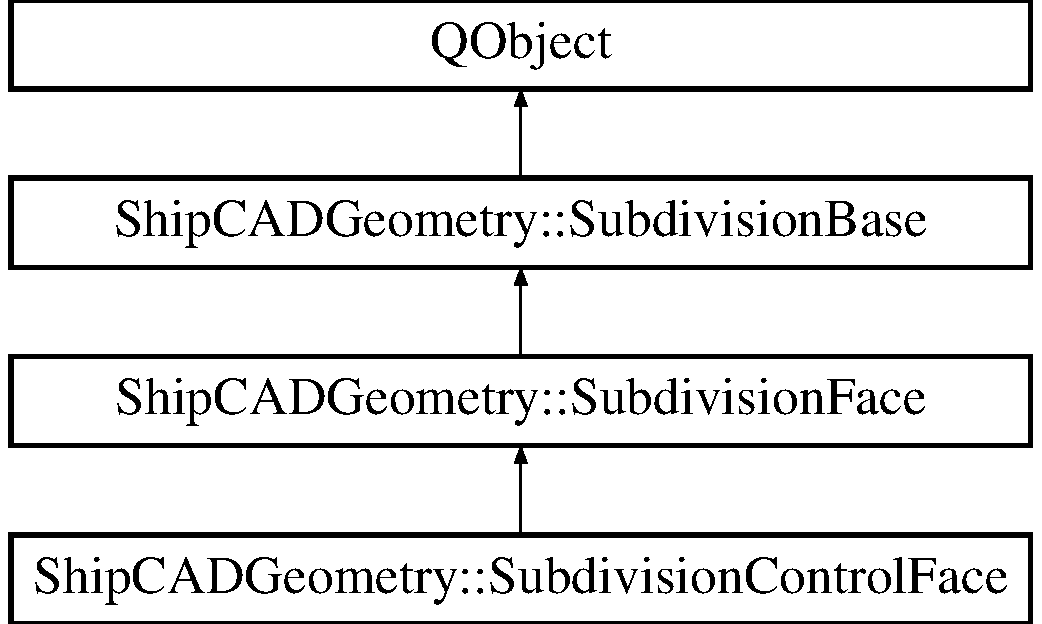
\includegraphics[height=4.000000cm]{classShipCADGeometry_1_1SubdivisionFace}
\end{center}
\end{figure}
\subsection*{Public Member Functions}
\begin{DoxyCompactItemize}
\item 
\hyperlink{classShipCADGeometry_1_1SubdivisionFace_a082f81f7a5750f7e53ed5a92ddc82350}{Subdivision\-Face} (\hyperlink{classShipCADGeometry_1_1SubdivisionSurface}{Subdivision\-Surface} $\ast$owner)
\item 
virtual \hyperlink{classShipCADGeometry_1_1SubdivisionFace_a44a0acc598533bf6846e4f7272e5c191}{$\sim$\-Subdivision\-Face} ()
\item 
void \hyperlink{classShipCADGeometry_1_1SubdivisionFace_a16d5e005d1c7c847ccf9ba72b67142fa}{flip\-Normal} ()
\item 
void \hyperlink{classShipCADGeometry_1_1SubdivisionFace_a553df49a1137f89d2df2846ffca74842}{add\-Point} (\hyperlink{classShipCADGeometry_1_1SubdivisionPoint}{Subdivision\-Point} $\ast$point)
\item 
void \hyperlink{classShipCADGeometry_1_1SubdivisionFace_aacd383eb085c4f6b92db89e25be6b3a1}{insert\-Point} (size\-\_\-t index, \hyperlink{classShipCADGeometry_1_1SubdivisionPoint}{Subdivision\-Point} $\ast$point)
\item 
virtual void \hyperlink{classShipCADGeometry_1_1SubdivisionFace_a413ae7e76f559780c8a69e998974fb75}{clear} ()
\begin{DoxyCompactList}\small\item\em reset this element to default values \end{DoxyCompactList}\item 
virtual void \hyperlink{classShipCADGeometry_1_1SubdivisionFace_a934edbf44e524a2ec250f896c3cc182d}{subdivide} (bool controlface, std\-::vector$<$ std\-::pair$<$ \hyperlink{classShipCADGeometry_1_1SubdivisionPoint}{Subdivision\-Point} $\ast$, \hyperlink{classShipCADGeometry_1_1SubdivisionPoint}{Subdivision\-Point} $\ast$ $>$ $>$ \&vertexpoints, std\-::vector$<$ std\-::pair$<$ \hyperlink{classShipCADGeometry_1_1SubdivisionEdge}{Subdivision\-Edge} $\ast$, \hyperlink{classShipCADGeometry_1_1SubdivisionPoint}{Subdivision\-Point} $\ast$ $>$ $>$ \&edgepoints, std\-::vector$<$ std\-::pair$<$ \hyperlink{classShipCADGeometry_1_1SubdivisionFace}{Subdivision\-Face} $\ast$, \hyperlink{classShipCADGeometry_1_1SubdivisionPoint}{Subdivision\-Point} $\ast$ $>$ $>$ \&facepoints, std\-::vector$<$ \hyperlink{classShipCADGeometry_1_1SubdivisionEdge}{Subdivision\-Edge} $\ast$ $>$ \&interioredges, std\-::vector$<$ \hyperlink{classShipCADGeometry_1_1SubdivisionEdge}{Subdivision\-Edge} $\ast$ $>$ \&controledges, std\-::vector$<$ \hyperlink{classShipCADGeometry_1_1SubdivisionFace}{Subdivision\-Face} $\ast$ $>$ \&dest)
\item 
size\-\_\-t \hyperlink{classShipCADGeometry_1_1SubdivisionFace_acb8b1174cf96615f4e84ca4e62f5979c}{number\-Of\-Points} ()
\item 
bool \hyperlink{classShipCADGeometry_1_1SubdivisionFace_a575f9199178fc28c9229fa4c7d2824ef}{has\-Point} (\hyperlink{classShipCADGeometry_1_1SubdivisionPoint}{Subdivision\-Point} $\ast$pt)
\item 
\hyperlink{classShipCADGeometry_1_1SubdivisionPoint}{Subdivision\-Point} $\ast$ \hyperlink{classShipCADGeometry_1_1SubdivisionFace_a0df579a3063c124ca2355eba4ece7480}{get\-Point} (size\-\_\-t index)
\begin{DoxyCompactList}\small\item\em get face point \end{DoxyCompactList}\item 
\hyperlink{classShipCADGeometry_1_1SubdivisionPoint}{Subdivision\-Point} $\ast$ \hyperlink{classShipCADGeometry_1_1SubdivisionFace_aeb9c6f01f3896dc39819265922a04892}{calculate\-Face\-Point} ()
\begin{DoxyCompactList}\small\item\em Get point on center of face for subdivision. \end{DoxyCompactList}\item 
size\-\_\-t \hyperlink{classShipCADGeometry_1_1SubdivisionFace_a8b32525b95c836e065cb124a61caec61}{index\-Of\-Point} (\hyperlink{classShipCADGeometry_1_1SubdivisionPoint}{Subdivision\-Point} $\ast$pt)
\begin{DoxyCompactList}\small\item\em get index of point in parent surface \end{DoxyCompactList}\item 
float \hyperlink{classShipCADGeometry_1_1SubdivisionFace_ace99f0fe3b54e57912e5391e0aff84ea}{get\-Area} ()
\item 
Q\-Vector3\-D \hyperlink{classShipCADGeometry_1_1SubdivisionFace_a3574fd6a4241a81faa7f2ff741d07811}{get\-Face\-Center} ()
\item 
Q\-Vector3\-D \hyperlink{classShipCADGeometry_1_1SubdivisionFace_add361089333f9d08a411d16ea1782246}{get\-Face\-Normal} ()
\item 
virtual void \hyperlink{classShipCADGeometry_1_1SubdivisionFace_aa5bd261ae5fc0a1c7fe8cc5328b8477f}{dump} (std\-::ostream \&os, const char $\ast$prefix=\char`\"{}\char`\"{}) const 
\begin{DoxyCompactList}\small\item\em print out the element to a stream \end{DoxyCompactList}\end{DoxyCompactItemize}
\subsection*{Static Public Member Functions}
\begin{DoxyCompactItemize}
\item 
static \hyperlink{classShipCADGeometry_1_1SubdivisionFace}{Subdivision\-Face} $\ast$ \hyperlink{classShipCADGeometry_1_1SubdivisionFace_a4a6f182fa7e5cf63fc95c7614805f136}{construct} (\hyperlink{classShipCADGeometry_1_1SubdivisionSurface}{Subdivision\-Surface} $\ast$owner)
\end{DoxyCompactItemize}
\subsection*{Protected Member Functions}
\begin{DoxyCompactItemize}
\item 
void \hyperlink{classShipCADGeometry_1_1SubdivisionFace_ab2f647963b552728f40d8c329318676e}{priv\-\_\-dump} (std\-::ostream \&os, const char $\ast$prefix) const 
\item 
void \hyperlink{classShipCADGeometry_1_1SubdivisionFace_a5399f7ec8ed458f6dbc733688c006cf8}{edge\-Check} (\hyperlink{classShipCADGeometry_1_1SubdivisionPoint}{Subdivision\-Point} $\ast$p1, \hyperlink{classShipCADGeometry_1_1SubdivisionPoint}{Subdivision\-Point} $\ast$p2, bool crease, bool controledge, \hyperlink{classShipCADGeometry_1_1SubdivisionControlCurve}{Subdivision\-Control\-Curve} $\ast$curve, std\-::vector$<$ \hyperlink{classShipCADGeometry_1_1SubdivisionEdge}{Subdivision\-Edge} $\ast$ $>$ \&interioredges, std\-::vector$<$ \hyperlink{classShipCADGeometry_1_1SubdivisionEdge}{Subdivision\-Edge} $\ast$ $>$ \&controledges)
\begin{DoxyCompactList}\small\item\em check for edge between points \end{DoxyCompactList}\end{DoxyCompactItemize}
\subsection*{Protected Attributes}
\begin{DoxyCompactItemize}
\item 
std\-::vector$<$ \hyperlink{classShipCADGeometry_1_1SubdivisionPoint}{Subdivision\-Point} $\ast$ $>$ \hyperlink{classShipCADGeometry_1_1SubdivisionFace_a1442d01623618d3bd3d231ac2f61bdf2}{\-\_\-points}
\end{DoxyCompactItemize}
\subsection*{Properties}
\begin{DoxyCompactItemize}
\item 
float \hyperlink{classShipCADGeometry_1_1SubdivisionFace_a19d38604a7e9f14c927c59616bb3b8a5}{Area}
\item 
Q\-Vector3\-D \hyperlink{classShipCADGeometry_1_1SubdivisionFace_a4ceab979e8faacf6c8c10420fb720080}{Face\-Center}
\item 
Q\-Vector3\-D \hyperlink{classShipCADGeometry_1_1SubdivisionFace_a4d9b9545d88ed7c470eadd42172c7530}{Face\-Normal}
\end{DoxyCompactItemize}


\subsection{Detailed Description}


Definition at line 56 of file subdivface.\-h.



\subsection{Constructor \& Destructor Documentation}
\hypertarget{classShipCADGeometry_1_1SubdivisionFace_a082f81f7a5750f7e53ed5a92ddc82350}{\index{Ship\-C\-A\-D\-Geometry\-::\-Subdivision\-Face@{Ship\-C\-A\-D\-Geometry\-::\-Subdivision\-Face}!Subdivision\-Face@{Subdivision\-Face}}
\index{Subdivision\-Face@{Subdivision\-Face}!ShipCADGeometry::SubdivisionFace@{Ship\-C\-A\-D\-Geometry\-::\-Subdivision\-Face}}
\subsubsection[{Subdivision\-Face}]{\setlength{\rightskip}{0pt plus 5cm}Subdivision\-Face\-::\-Subdivision\-Face (
\begin{DoxyParamCaption}
\item[{{\bf Subdivision\-Surface} $\ast$}]{owner}
\end{DoxyParamCaption}
)\hspace{0.3cm}{\ttfamily [explicit]}}}\label{classShipCADGeometry_1_1SubdivisionFace_a082f81f7a5750f7e53ed5a92ddc82350}


Definition at line 61 of file subdivface.\-cpp.

\hypertarget{classShipCADGeometry_1_1SubdivisionFace_a44a0acc598533bf6846e4f7272e5c191}{\index{Ship\-C\-A\-D\-Geometry\-::\-Subdivision\-Face@{Ship\-C\-A\-D\-Geometry\-::\-Subdivision\-Face}!$\sim$\-Subdivision\-Face@{$\sim$\-Subdivision\-Face}}
\index{$\sim$\-Subdivision\-Face@{$\sim$\-Subdivision\-Face}!ShipCADGeometry::SubdivisionFace@{Ship\-C\-A\-D\-Geometry\-::\-Subdivision\-Face}}
\subsubsection[{$\sim$\-Subdivision\-Face}]{\setlength{\rightskip}{0pt plus 5cm}Subdivision\-Face\-::$\sim$\-Subdivision\-Face (
\begin{DoxyParamCaption}
{}
\end{DoxyParamCaption}
)\hspace{0.3cm}{\ttfamily [virtual]}}}\label{classShipCADGeometry_1_1SubdivisionFace_a44a0acc598533bf6846e4f7272e5c191}


Definition at line 67 of file subdivface.\-cpp.



\subsection{Member Function Documentation}
\hypertarget{classShipCADGeometry_1_1SubdivisionFace_a553df49a1137f89d2df2846ffca74842}{\index{Ship\-C\-A\-D\-Geometry\-::\-Subdivision\-Face@{Ship\-C\-A\-D\-Geometry\-::\-Subdivision\-Face}!add\-Point@{add\-Point}}
\index{add\-Point@{add\-Point}!ShipCADGeometry::SubdivisionFace@{Ship\-C\-A\-D\-Geometry\-::\-Subdivision\-Face}}
\subsubsection[{add\-Point}]{\setlength{\rightskip}{0pt plus 5cm}void Subdivision\-Face\-::add\-Point (
\begin{DoxyParamCaption}
\item[{{\bf Subdivision\-Point} $\ast$}]{point}
\end{DoxyParamCaption}
)}}\label{classShipCADGeometry_1_1SubdivisionFace_a553df49a1137f89d2df2846ffca74842}


Definition at line 159 of file subdivface.\-cpp.

\hypertarget{classShipCADGeometry_1_1SubdivisionFace_aeb9c6f01f3896dc39819265922a04892}{\index{Ship\-C\-A\-D\-Geometry\-::\-Subdivision\-Face@{Ship\-C\-A\-D\-Geometry\-::\-Subdivision\-Face}!calculate\-Face\-Point@{calculate\-Face\-Point}}
\index{calculate\-Face\-Point@{calculate\-Face\-Point}!ShipCADGeometry::SubdivisionFace@{Ship\-C\-A\-D\-Geometry\-::\-Subdivision\-Face}}
\subsubsection[{calculate\-Face\-Point}]{\setlength{\rightskip}{0pt plus 5cm}{\bf Subdivision\-Point} $\ast$ Subdivision\-Face\-::calculate\-Face\-Point (
\begin{DoxyParamCaption}
{}
\end{DoxyParamCaption}
)}}\label{classShipCADGeometry_1_1SubdivisionFace_aeb9c6f01f3896dc39819265922a04892}


Get point on center of face for subdivision. 

When subdividing a face, each edge is split, and a point is put in the center of the face, then all are connected and new faces created. If the face is a triangle and we are not using fv\-Catmull\-Clark, then a center point is not created. The face is then divided into triangles, instead of quadrilateral faces. In that case this returns a null point

\begin{DoxyReturn}{Returns}
the point at center of face, or 0 if triangle and not using fv\-Catmull\-Clark, or the number of face points is less than 3 
\end{DoxyReturn}


Definition at line 165 of file subdivface.\-cpp.

\hypertarget{classShipCADGeometry_1_1SubdivisionFace_a413ae7e76f559780c8a69e998974fb75}{\index{Ship\-C\-A\-D\-Geometry\-::\-Subdivision\-Face@{Ship\-C\-A\-D\-Geometry\-::\-Subdivision\-Face}!clear@{clear}}
\index{clear@{clear}!ShipCADGeometry::SubdivisionFace@{Ship\-C\-A\-D\-Geometry\-::\-Subdivision\-Face}}
\subsubsection[{clear}]{\setlength{\rightskip}{0pt plus 5cm}void Subdivision\-Face\-::clear (
\begin{DoxyParamCaption}
{}
\end{DoxyParamCaption}
)\hspace{0.3cm}{\ttfamily [virtual]}}}\label{classShipCADGeometry_1_1SubdivisionFace_a413ae7e76f559780c8a69e998974fb75}


reset this element to default values 



Implements \hyperlink{classShipCADGeometry_1_1SubdivisionBase_ae668920d97c0810c72996a531e0ca107}{Ship\-C\-A\-D\-Geometry\-::\-Subdivision\-Base}.



Reimplemented in \hyperlink{classShipCADGeometry_1_1SubdivisionControlFace_ad168e31f0ef2537b3cd0f58b0c1c54e2}{Ship\-C\-A\-D\-Geometry\-::\-Subdivision\-Control\-Face}.



Definition at line 183 of file subdivface.\-cpp.

\hypertarget{classShipCADGeometry_1_1SubdivisionFace_a4a6f182fa7e5cf63fc95c7614805f136}{\index{Ship\-C\-A\-D\-Geometry\-::\-Subdivision\-Face@{Ship\-C\-A\-D\-Geometry\-::\-Subdivision\-Face}!construct@{construct}}
\index{construct@{construct}!ShipCADGeometry::SubdivisionFace@{Ship\-C\-A\-D\-Geometry\-::\-Subdivision\-Face}}
\subsubsection[{construct}]{\setlength{\rightskip}{0pt plus 5cm}{\bf Subdivision\-Face} $\ast$ Subdivision\-Face\-::construct (
\begin{DoxyParamCaption}
\item[{{\bf Subdivision\-Surface} $\ast$}]{owner}
\end{DoxyParamCaption}
)\hspace{0.3cm}{\ttfamily [static]}}}\label{classShipCADGeometry_1_1SubdivisionFace_a4a6f182fa7e5cf63fc95c7614805f136}


Definition at line 53 of file subdivface.\-cpp.

\hypertarget{classShipCADGeometry_1_1SubdivisionFace_aa5bd261ae5fc0a1c7fe8cc5328b8477f}{\index{Ship\-C\-A\-D\-Geometry\-::\-Subdivision\-Face@{Ship\-C\-A\-D\-Geometry\-::\-Subdivision\-Face}!dump@{dump}}
\index{dump@{dump}!ShipCADGeometry::SubdivisionFace@{Ship\-C\-A\-D\-Geometry\-::\-Subdivision\-Face}}
\subsubsection[{dump}]{\setlength{\rightskip}{0pt plus 5cm}void Subdivision\-Face\-::dump (
\begin{DoxyParamCaption}
\item[{std\-::ostream \&}]{os, }
\item[{const char $\ast$}]{prefix = {\ttfamily \char`\"{}\char`\"{}}}
\end{DoxyParamCaption}
) const\hspace{0.3cm}{\ttfamily [virtual]}}}\label{classShipCADGeometry_1_1SubdivisionFace_aa5bd261ae5fc0a1c7fe8cc5328b8477f}


print out the element to a stream 


\begin{DoxyParams}{Parameters}
{\em os} & the output stream \\
\hline
{\em prefix} & string to prefix on each line output \\
\hline
\end{DoxyParams}


Reimplemented from \hyperlink{classShipCADGeometry_1_1SubdivisionBase_a7807e64ac8d2acc3da572e03cf0523b6}{Ship\-C\-A\-D\-Geometry\-::\-Subdivision\-Base}.



Reimplemented in \hyperlink{classShipCADGeometry_1_1SubdivisionControlFace_a947868fba3e9bb6c587847fb9245c9ff}{Ship\-C\-A\-D\-Geometry\-::\-Subdivision\-Control\-Face}.



Definition at line 384 of file subdivface.\-cpp.

\hypertarget{classShipCADGeometry_1_1SubdivisionFace_a5399f7ec8ed458f6dbc733688c006cf8}{\index{Ship\-C\-A\-D\-Geometry\-::\-Subdivision\-Face@{Ship\-C\-A\-D\-Geometry\-::\-Subdivision\-Face}!edge\-Check@{edge\-Check}}
\index{edge\-Check@{edge\-Check}!ShipCADGeometry::SubdivisionFace@{Ship\-C\-A\-D\-Geometry\-::\-Subdivision\-Face}}
\subsubsection[{edge\-Check}]{\setlength{\rightskip}{0pt plus 5cm}void Subdivision\-Face\-::edge\-Check (
\begin{DoxyParamCaption}
\item[{{\bf Subdivision\-Point} $\ast$}]{p1, }
\item[{{\bf Subdivision\-Point} $\ast$}]{p2, }
\item[{bool}]{crease, }
\item[{bool}]{controledge, }
\item[{{\bf Subdivision\-Control\-Curve} $\ast$}]{curve, }
\item[{std\-::vector$<$ {\bf Subdivision\-Edge} $\ast$ $>$ \&}]{interioredges, }
\item[{std\-::vector$<$ {\bf Subdivision\-Edge} $\ast$ $>$ \&}]{controledges}
\end{DoxyParamCaption}
)\hspace{0.3cm}{\ttfamily [protected]}}}\label{classShipCADGeometry_1_1SubdivisionFace_a5399f7ec8ed458f6dbc733688c006cf8}


check for edge between points 

This method will create edges between 2 points if it doesn't exist.


\begin{DoxyParams}{Parameters}
{\em p1} & start point of edge \\
\hline
{\em p2} & end point of edge \\
\hline
{\em crease} & whether this edge is a crease \\
\hline
{\em controledge} & whether this edge is a control edge \\
\hline
{\em curve} & if edge is a controledge, then pass the curve to be attached \\
\hline
{\em interioredges} & if this edge is an interior edge, add it to this list \\
\hline
{\em controledges} & if this edge is a control, add it to this list \\
\hline
\end{DoxyParams}


Definition at line 197 of file subdivface.\-cpp.

\hypertarget{classShipCADGeometry_1_1SubdivisionFace_a16d5e005d1c7c847ccf9ba72b67142fa}{\index{Ship\-C\-A\-D\-Geometry\-::\-Subdivision\-Face@{Ship\-C\-A\-D\-Geometry\-::\-Subdivision\-Face}!flip\-Normal@{flip\-Normal}}
\index{flip\-Normal@{flip\-Normal}!ShipCADGeometry::SubdivisionFace@{Ship\-C\-A\-D\-Geometry\-::\-Subdivision\-Face}}
\subsubsection[{flip\-Normal}]{\setlength{\rightskip}{0pt plus 5cm}void Subdivision\-Face\-::flip\-Normal (
\begin{DoxyParamCaption}
{}
\end{DoxyParamCaption}
)}}\label{classShipCADGeometry_1_1SubdivisionFace_a16d5e005d1c7c847ccf9ba72b67142fa}


Definition at line 188 of file subdivface.\-cpp.

\hypertarget{classShipCADGeometry_1_1SubdivisionFace_ace99f0fe3b54e57912e5391e0aff84ea}{\index{Ship\-C\-A\-D\-Geometry\-::\-Subdivision\-Face@{Ship\-C\-A\-D\-Geometry\-::\-Subdivision\-Face}!get\-Area@{get\-Area}}
\index{get\-Area@{get\-Area}!ShipCADGeometry::SubdivisionFace@{Ship\-C\-A\-D\-Geometry\-::\-Subdivision\-Face}}
\subsubsection[{get\-Area}]{\setlength{\rightskip}{0pt plus 5cm}float Subdivision\-Face\-::get\-Area (
\begin{DoxyParamCaption}
{}
\end{DoxyParamCaption}
)}}\label{classShipCADGeometry_1_1SubdivisionFace_ace99f0fe3b54e57912e5391e0aff84ea}


Definition at line 98 of file subdivface.\-cpp.

\hypertarget{classShipCADGeometry_1_1SubdivisionFace_a3574fd6a4241a81faa7f2ff741d07811}{\index{Ship\-C\-A\-D\-Geometry\-::\-Subdivision\-Face@{Ship\-C\-A\-D\-Geometry\-::\-Subdivision\-Face}!get\-Face\-Center@{get\-Face\-Center}}
\index{get\-Face\-Center@{get\-Face\-Center}!ShipCADGeometry::SubdivisionFace@{Ship\-C\-A\-D\-Geometry\-::\-Subdivision\-Face}}
\subsubsection[{get\-Face\-Center}]{\setlength{\rightskip}{0pt plus 5cm}Q\-Vector3\-D Subdivision\-Face\-::get\-Face\-Center (
\begin{DoxyParamCaption}
{}
\end{DoxyParamCaption}
)}}\label{classShipCADGeometry_1_1SubdivisionFace_a3574fd6a4241a81faa7f2ff741d07811}


Definition at line 108 of file subdivface.\-cpp.

\hypertarget{classShipCADGeometry_1_1SubdivisionFace_add361089333f9d08a411d16ea1782246}{\index{Ship\-C\-A\-D\-Geometry\-::\-Subdivision\-Face@{Ship\-C\-A\-D\-Geometry\-::\-Subdivision\-Face}!get\-Face\-Normal@{get\-Face\-Normal}}
\index{get\-Face\-Normal@{get\-Face\-Normal}!ShipCADGeometry::SubdivisionFace@{Ship\-C\-A\-D\-Geometry\-::\-Subdivision\-Face}}
\subsubsection[{get\-Face\-Normal}]{\setlength{\rightskip}{0pt plus 5cm}Q\-Vector3\-D Subdivision\-Face\-::get\-Face\-Normal (
\begin{DoxyParamCaption}
{}
\end{DoxyParamCaption}
)}}\label{classShipCADGeometry_1_1SubdivisionFace_add361089333f9d08a411d16ea1782246}


Definition at line 121 of file subdivface.\-cpp.

\hypertarget{classShipCADGeometry_1_1SubdivisionFace_a0df579a3063c124ca2355eba4ece7480}{\index{Ship\-C\-A\-D\-Geometry\-::\-Subdivision\-Face@{Ship\-C\-A\-D\-Geometry\-::\-Subdivision\-Face}!get\-Point@{get\-Point}}
\index{get\-Point@{get\-Point}!ShipCADGeometry::SubdivisionFace@{Ship\-C\-A\-D\-Geometry\-::\-Subdivision\-Face}}
\subsubsection[{get\-Point}]{\setlength{\rightskip}{0pt plus 5cm}{\bf Subdivision\-Point} $\ast$ Subdivision\-Face\-::get\-Point (
\begin{DoxyParamCaption}
\item[{size\-\_\-t}]{index}
\end{DoxyParamCaption}
)}}\label{classShipCADGeometry_1_1SubdivisionFace_a0df579a3063c124ca2355eba4ece7480}


get face point 


\begin{DoxyParams}{Parameters}
{\em index} & index of point to get \\
\hline
\end{DoxyParams}
\begin{DoxyReturn}{Returns}
the point at index 
\end{DoxyReturn}


Definition at line 152 of file subdivface.\-cpp.

\hypertarget{classShipCADGeometry_1_1SubdivisionFace_a575f9199178fc28c9229fa4c7d2824ef}{\index{Ship\-C\-A\-D\-Geometry\-::\-Subdivision\-Face@{Ship\-C\-A\-D\-Geometry\-::\-Subdivision\-Face}!has\-Point@{has\-Point}}
\index{has\-Point@{has\-Point}!ShipCADGeometry::SubdivisionFace@{Ship\-C\-A\-D\-Geometry\-::\-Subdivision\-Face}}
\subsubsection[{has\-Point}]{\setlength{\rightskip}{0pt plus 5cm}bool Subdivision\-Face\-::has\-Point (
\begin{DoxyParamCaption}
\item[{{\bf Subdivision\-Point} $\ast$}]{pt}
\end{DoxyParamCaption}
)}}\label{classShipCADGeometry_1_1SubdivisionFace_a575f9199178fc28c9229fa4c7d2824ef}


Definition at line 147 of file subdivface.\-cpp.

\hypertarget{classShipCADGeometry_1_1SubdivisionFace_a8b32525b95c836e065cb124a61caec61}{\index{Ship\-C\-A\-D\-Geometry\-::\-Subdivision\-Face@{Ship\-C\-A\-D\-Geometry\-::\-Subdivision\-Face}!index\-Of\-Point@{index\-Of\-Point}}
\index{index\-Of\-Point@{index\-Of\-Point}!ShipCADGeometry::SubdivisionFace@{Ship\-C\-A\-D\-Geometry\-::\-Subdivision\-Face}}
\subsubsection[{index\-Of\-Point}]{\setlength{\rightskip}{0pt plus 5cm}size\-\_\-t Subdivision\-Face\-::index\-Of\-Point (
\begin{DoxyParamCaption}
\item[{{\bf Subdivision\-Point} $\ast$}]{pt}
\end{DoxyParamCaption}
)}}\label{classShipCADGeometry_1_1SubdivisionFace_a8b32525b95c836e065cb124a61caec61}


get index of point in parent surface 


\begin{DoxyParams}{Parameters}
{\em pt} & point to find in parent surface \\
\hline
\end{DoxyParams}
\begin{DoxyReturn}{Returns}
index of that point in parent surface 
\end{DoxyReturn}


Definition at line 72 of file subdivface.\-cpp.

\hypertarget{classShipCADGeometry_1_1SubdivisionFace_aacd383eb085c4f6b92db89e25be6b3a1}{\index{Ship\-C\-A\-D\-Geometry\-::\-Subdivision\-Face@{Ship\-C\-A\-D\-Geometry\-::\-Subdivision\-Face}!insert\-Point@{insert\-Point}}
\index{insert\-Point@{insert\-Point}!ShipCADGeometry::SubdivisionFace@{Ship\-C\-A\-D\-Geometry\-::\-Subdivision\-Face}}
\subsubsection[{insert\-Point}]{\setlength{\rightskip}{0pt plus 5cm}void Subdivision\-Face\-::insert\-Point (
\begin{DoxyParamCaption}
\item[{size\-\_\-t}]{index, }
\item[{{\bf Subdivision\-Point} $\ast$}]{point}
\end{DoxyParamCaption}
)}}\label{classShipCADGeometry_1_1SubdivisionFace_aacd383eb085c4f6b92db89e25be6b3a1}


Definition at line 77 of file subdivface.\-cpp.

\hypertarget{classShipCADGeometry_1_1SubdivisionFace_acb8b1174cf96615f4e84ca4e62f5979c}{\index{Ship\-C\-A\-D\-Geometry\-::\-Subdivision\-Face@{Ship\-C\-A\-D\-Geometry\-::\-Subdivision\-Face}!number\-Of\-Points@{number\-Of\-Points}}
\index{number\-Of\-Points@{number\-Of\-Points}!ShipCADGeometry::SubdivisionFace@{Ship\-C\-A\-D\-Geometry\-::\-Subdivision\-Face}}
\subsubsection[{number\-Of\-Points}]{\setlength{\rightskip}{0pt plus 5cm}size\-\_\-t Ship\-C\-A\-D\-Geometry\-::\-Subdivision\-Face\-::number\-Of\-Points (
\begin{DoxyParamCaption}
{}
\end{DoxyParamCaption}
)\hspace{0.3cm}{\ttfamily [inline]}}}\label{classShipCADGeometry_1_1SubdivisionFace_acb8b1174cf96615f4e84ca4e62f5979c}


Definition at line 83 of file subdivface.\-h.

\hypertarget{classShipCADGeometry_1_1SubdivisionFace_ab2f647963b552728f40d8c329318676e}{\index{Ship\-C\-A\-D\-Geometry\-::\-Subdivision\-Face@{Ship\-C\-A\-D\-Geometry\-::\-Subdivision\-Face}!priv\-\_\-dump@{priv\-\_\-dump}}
\index{priv\-\_\-dump@{priv\-\_\-dump}!ShipCADGeometry::SubdivisionFace@{Ship\-C\-A\-D\-Geometry\-::\-Subdivision\-Face}}
\subsubsection[{priv\-\_\-dump}]{\setlength{\rightskip}{0pt plus 5cm}void Subdivision\-Face\-::priv\-\_\-dump (
\begin{DoxyParamCaption}
\item[{std\-::ostream \&}]{os, }
\item[{const char $\ast$}]{prefix}
\end{DoxyParamCaption}
) const\hspace{0.3cm}{\ttfamily [protected]}}}\label{classShipCADGeometry_1_1SubdivisionFace_ab2f647963b552728f40d8c329318676e}


Definition at line 391 of file subdivface.\-cpp.

\hypertarget{classShipCADGeometry_1_1SubdivisionFace_a934edbf44e524a2ec250f896c3cc182d}{\index{Ship\-C\-A\-D\-Geometry\-::\-Subdivision\-Face@{Ship\-C\-A\-D\-Geometry\-::\-Subdivision\-Face}!subdivide@{subdivide}}
\index{subdivide@{subdivide}!ShipCADGeometry::SubdivisionFace@{Ship\-C\-A\-D\-Geometry\-::\-Subdivision\-Face}}
\subsubsection[{subdivide}]{\setlength{\rightskip}{0pt plus 5cm}void Subdivision\-Face\-::subdivide (
\begin{DoxyParamCaption}
\item[{bool}]{controlface, }
\item[{std\-::vector$<$ std\-::pair$<$ {\bf Subdivision\-Point} $\ast$, {\bf Subdivision\-Point} $\ast$ $>$ $>$ \&}]{vertexpoints, }
\item[{std\-::vector$<$ std\-::pair$<$ {\bf Subdivision\-Edge} $\ast$, {\bf Subdivision\-Point} $\ast$ $>$ $>$ \&}]{edgepoints, }
\item[{std\-::vector$<$ std\-::pair$<$ {\bf Subdivision\-Face} $\ast$, {\bf Subdivision\-Point} $\ast$ $>$ $>$ \&}]{facepoints, }
\item[{std\-::vector$<$ {\bf Subdivision\-Edge} $\ast$ $>$ \&}]{interioredges, }
\item[{std\-::vector$<$ {\bf Subdivision\-Edge} $\ast$ $>$ \&}]{controledges, }
\item[{std\-::vector$<$ {\bf Subdivision\-Face} $\ast$ $>$ \&}]{dest}
\end{DoxyParamCaption}
)\hspace{0.3cm}{\ttfamily [virtual]}}}\label{classShipCADGeometry_1_1SubdivisionFace_a934edbf44e524a2ec250f896c3cc182d}


Definition at line 259 of file subdivface.\-cpp.



\subsection{Member Data Documentation}
\hypertarget{classShipCADGeometry_1_1SubdivisionFace_a1442d01623618d3bd3d231ac2f61bdf2}{\index{Ship\-C\-A\-D\-Geometry\-::\-Subdivision\-Face@{Ship\-C\-A\-D\-Geometry\-::\-Subdivision\-Face}!\-\_\-points@{\-\_\-points}}
\index{\-\_\-points@{\-\_\-points}!ShipCADGeometry::SubdivisionFace@{Ship\-C\-A\-D\-Geometry\-::\-Subdivision\-Face}}
\subsubsection[{\-\_\-points}]{\setlength{\rightskip}{0pt plus 5cm}std\-::vector$<${\bf Subdivision\-Point}$\ast$$>$ Ship\-C\-A\-D\-Geometry\-::\-Subdivision\-Face\-::\-\_\-points\hspace{0.3cm}{\ttfamily [protected]}}}\label{classShipCADGeometry_1_1SubdivisionFace_a1442d01623618d3bd3d231ac2f61bdf2}


Definition at line 146 of file subdivface.\-h.



\subsection{Property Documentation}
\hypertarget{classShipCADGeometry_1_1SubdivisionFace_a19d38604a7e9f14c927c59616bb3b8a5}{\index{Ship\-C\-A\-D\-Geometry\-::\-Subdivision\-Face@{Ship\-C\-A\-D\-Geometry\-::\-Subdivision\-Face}!Area@{Area}}
\index{Area@{Area}!ShipCADGeometry::SubdivisionFace@{Ship\-C\-A\-D\-Geometry\-::\-Subdivision\-Face}}
\subsubsection[{Area}]{\setlength{\rightskip}{0pt plus 5cm}float Ship\-C\-A\-D\-Geometry\-::\-Subdivision\-Face\-::\-Area\hspace{0.3cm}{\ttfamily [read]}}}\label{classShipCADGeometry_1_1SubdivisionFace_a19d38604a7e9f14c927c59616bb3b8a5}


Definition at line 59 of file subdivface.\-h.

\hypertarget{classShipCADGeometry_1_1SubdivisionFace_a4ceab979e8faacf6c8c10420fb720080}{\index{Ship\-C\-A\-D\-Geometry\-::\-Subdivision\-Face@{Ship\-C\-A\-D\-Geometry\-::\-Subdivision\-Face}!Face\-Center@{Face\-Center}}
\index{Face\-Center@{Face\-Center}!ShipCADGeometry::SubdivisionFace@{Ship\-C\-A\-D\-Geometry\-::\-Subdivision\-Face}}
\subsubsection[{Face\-Center}]{\setlength{\rightskip}{0pt plus 5cm}Q\-Vector3\-D Ship\-C\-A\-D\-Geometry\-::\-Subdivision\-Face\-::\-Face\-Center\hspace{0.3cm}{\ttfamily [read]}}}\label{classShipCADGeometry_1_1SubdivisionFace_a4ceab979e8faacf6c8c10420fb720080}


Definition at line 60 of file subdivface.\-h.

\hypertarget{classShipCADGeometry_1_1SubdivisionFace_a4d9b9545d88ed7c470eadd42172c7530}{\index{Ship\-C\-A\-D\-Geometry\-::\-Subdivision\-Face@{Ship\-C\-A\-D\-Geometry\-::\-Subdivision\-Face}!Face\-Normal@{Face\-Normal}}
\index{Face\-Normal@{Face\-Normal}!ShipCADGeometry::SubdivisionFace@{Ship\-C\-A\-D\-Geometry\-::\-Subdivision\-Face}}
\subsubsection[{Face\-Normal}]{\setlength{\rightskip}{0pt plus 5cm}Q\-Vector3\-D Ship\-C\-A\-D\-Geometry\-::\-Subdivision\-Face\-::\-Face\-Normal\hspace{0.3cm}{\ttfamily [read]}}}\label{classShipCADGeometry_1_1SubdivisionFace_a4d9b9545d88ed7c470eadd42172c7530}


Definition at line 61 of file subdivface.\-h.



The documentation for this class was generated from the following files\-:\begin{DoxyCompactItemize}
\item 
Ship\-C\-A\-Dlib/\hyperlink{subdivface_8h}{subdivface.\-h}\item 
Ship\-C\-A\-Dlib/\hyperlink{subdivface_8cpp}{subdivface.\-cpp}\end{DoxyCompactItemize}

\hypertarget{classShipCADGeometry_1_1SubdivisionLayer}{\section{Ship\-C\-A\-D\-Geometry\-:\-:Subdivision\-Layer Class Reference}
\label{classShipCADGeometry_1_1SubdivisionLayer}\index{Ship\-C\-A\-D\-Geometry\-::\-Subdivision\-Layer@{Ship\-C\-A\-D\-Geometry\-::\-Subdivision\-Layer}}
}


{\ttfamily \#include $<$subdivlayer.\-h$>$}

Inheritance diagram for Ship\-C\-A\-D\-Geometry\-:\-:Subdivision\-Layer\-:\begin{figure}[H]
\begin{center}
\leavevmode
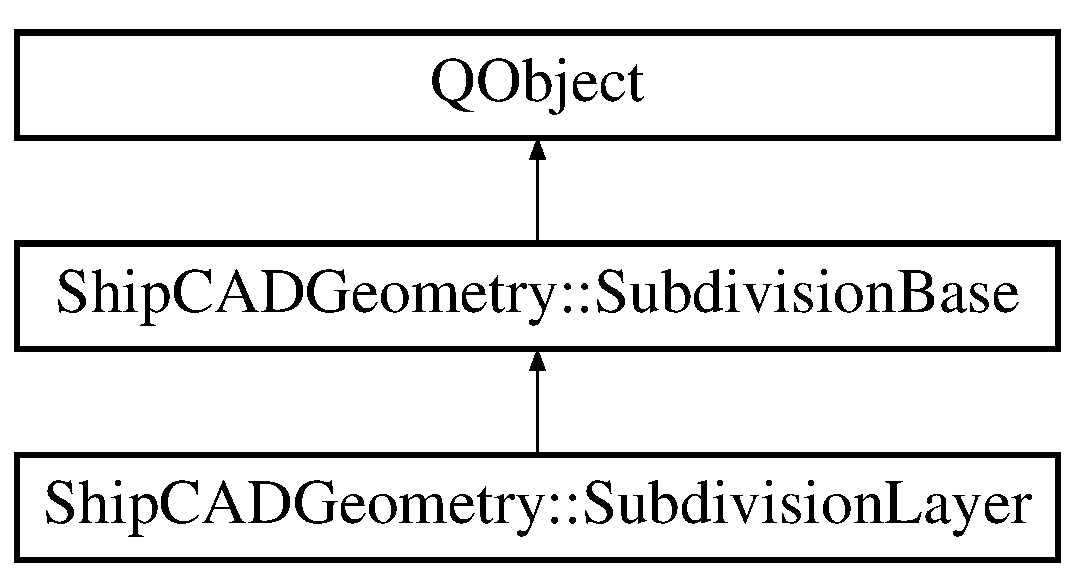
\includegraphics[height=3.000000cm]{classShipCADGeometry_1_1SubdivisionLayer}
\end{center}
\end{figure}
\subsection*{Signals}
\begin{DoxyCompactItemize}
\item 
void \hyperlink{classShipCADGeometry_1_1SubdivisionLayer_a92c3a056412b83396a30cd641bdfdceb}{changed\-Layer\-Data} (size\-\_\-t layerid)
\end{DoxyCompactItemize}
\subsection*{Public Member Functions}
\begin{DoxyCompactItemize}
\item 
\hyperlink{classShipCADGeometry_1_1SubdivisionLayer_a788864a40265b764b8d97d9a9cbbbd13}{Subdivision\-Layer} (\hyperlink{classShipCADGeometry_1_1SubdivisionSurface}{Subdivision\-Surface} $\ast$owner)
\item 
virtual \hyperlink{classShipCADGeometry_1_1SubdivisionLayer_a4e852a07f46e57f28ffedd4a68c2f4c4}{$\sim$\-Subdivision\-Layer} ()
\item 
void \hyperlink{classShipCADGeometry_1_1SubdivisionLayer_a45b3af65b8b11dd2bf566a454bc125bd}{delete\-Control\-Face} (\hyperlink{classShipCADGeometry_1_1SubdivisionControlFace}{Subdivision\-Control\-Face} $\ast$face)
\item 
void \hyperlink{classShipCADGeometry_1_1SubdivisionLayer_a3c966ebc7e2c1f516f2329324d5658e2}{add\-Control\-Face} (\hyperlink{classShipCADGeometry_1_1SubdivisionControlFace}{Subdivision\-Control\-Face} $\ast$newface)
\item 
size\-\_\-t \hyperlink{classShipCADGeometry_1_1SubdivisionLayer_ac25e800b3f77d61413272a06cb616813}{number\-Of\-Faces} ()
\item 
\hyperlink{classShipCADGeometry_1_1SubdivisionControlFace}{Subdivision\-Control\-Face} $\ast$ \hyperlink{classShipCADGeometry_1_1SubdivisionLayer_a2e1538a000268fe5f56bf2bea4973c23}{get\-Face} (size\-\_\-t index)
\item 
bool \hyperlink{classShipCADGeometry_1_1SubdivisionLayer_ab2d11ebf60ad6edd818eb0c42971946c}{calculate\-Intersection\-Points} (\hyperlink{classShipCADGeometry_1_1SubdivisionLayer}{Subdivision\-Layer} $\ast$layer)
\item 
virtual void \hyperlink{classShipCADGeometry_1_1SubdivisionLayer_a7046d17ba87dd5ce7399f22ae327fc6e}{clear} ()
\begin{DoxyCompactList}\small\item\em reset this element to default values \end{DoxyCompactList}\item 
void \hyperlink{classShipCADGeometry_1_1SubdivisionLayer_a319ae070f596e92307671cda0a607887}{assign\-Properties} (\hyperlink{classShipCADGeometry_1_1SubdivisionLayer}{Subdivision\-Layer} $\ast$source)
\item 
void \hyperlink{classShipCADGeometry_1_1SubdivisionLayer_a75d5f29031d9c93f291d370c79614e87}{move\-Down} ()
\item 
void \hyperlink{classShipCADGeometry_1_1SubdivisionLayer_aa5fc01f512f9d01f49e05c1608433654}{move\-Up} ()
\item 
void \hyperlink{classShipCADGeometry_1_1SubdivisionLayer_a2fc3ac326021a97479b821331e295640}{extents} (Q\-Vector3\-D \&min, Q\-Vector3\-D \&max)
\item 
\hyperlink{structShipCADGeometry_1_1LayerProperties}{Layer\-Properties} \hyperlink{classShipCADGeometry_1_1SubdivisionLayer_a7d42f81a94b46f0d999a4fa7a48d57d6}{get\-Surface\-Properties} ()
\item 
bool \hyperlink{classShipCADGeometry_1_1SubdivisionLayer_a6abf8365e77b1ebefbd5d03228efb2b5}{is\-Visible} ()
\item 
bool \hyperlink{classShipCADGeometry_1_1SubdivisionLayer_a48dfa484b555a964db080737cf2c5c0f}{is\-Symmetric} ()
\item 
bool \hyperlink{classShipCADGeometry_1_1SubdivisionLayer_a90a02f5cf0f49f47784e2f52a5283bbd}{is\-Developable} ()
\item 
bool \hyperlink{classShipCADGeometry_1_1SubdivisionLayer_a53e1ee753b64b7f08161e81901d6a7dd}{use\-For\-Intersections} ()
\item 
bool \hyperlink{classShipCADGeometry_1_1SubdivisionLayer_a3bf57aec73dfebdde5a6fb0a7596e2fb}{use\-In\-Hydrostatics} ()
\item 
bool \hyperlink{classShipCADGeometry_1_1SubdivisionLayer_affa6fc5b3ebb056b3e081372623c94c8}{show\-In\-Linesplan} ()
\item 
size\-\_\-t \hyperlink{classShipCADGeometry_1_1SubdivisionLayer_a422af89a2c4e8cdafd264fd54390ea85}{get\-Layer\-I\-D} ()
\item 
void \hyperlink{classShipCADGeometry_1_1SubdivisionLayer_afc09ab43011444cbb373114b7387b880}{set\-Layer\-I\-D} (size\-\_\-t newid)
\item 
size\-\_\-t \hyperlink{classShipCADGeometry_1_1SubdivisionLayer_a9a760dcc67779d111d5e05585e939138}{get\-Layer\-Index} ()
\item 
float \hyperlink{classShipCADGeometry_1_1SubdivisionLayer_aa7c79dd53c5c8c0a6ba3e0e8239013bc}{get\-Material\-Density} ()
\item 
float \hyperlink{classShipCADGeometry_1_1SubdivisionLayer_a824c050d58ae144e1f669ef84ed921be}{get\-Thickness} ()
\item 
Q\-String \hyperlink{classShipCADGeometry_1_1SubdivisionLayer_affb4df074a7f116ce60f51ad7b7ba230}{get\-Name} ()
\item 
Q\-String \hyperlink{classShipCADGeometry_1_1SubdivisionLayer_a0d4f8e0f8f99b18fc6bf5df0554d11ce}{get\-Description} ()
\item 
Q\-String \hyperlink{classShipCADGeometry_1_1SubdivisionLayer_a52e6b9f53d989156e073d5fdc820c968}{get\-D\-X\-F\-Layername} ()
\item 
Q\-Color \hyperlink{classShipCADGeometry_1_1SubdivisionLayer_aa1a348600f3ceea5b28569c683d445a5}{get\-Color} ()
\item 
float \hyperlink{classShipCADGeometry_1_1SubdivisionLayer_a34d50c0f49578ecfe8f228bc8d52be6f}{get\-Alpha\-Blend} ()
\item 
void \hyperlink{classShipCADGeometry_1_1SubdivisionLayer_a6fdfc0d208904d821349eb7380a52411}{set\-Developable} (bool val)
\item 
void \hyperlink{classShipCADGeometry_1_1SubdivisionLayer_a3e81d07f92749d57d84688b038f60946}{set\-Description} (const Q\-String \&val)
\item 
void \hyperlink{classShipCADGeometry_1_1SubdivisionLayer_a3861c77aeb283fbea6efe943ced83f41}{set\-Name} (const Q\-String \&val)
\item 
void \hyperlink{classShipCADGeometry_1_1SubdivisionLayer_ab3c7c5072ba6cd411404651e8e0dca2f}{set\-Symmetric} (bool val)
\item 
void \hyperlink{classShipCADGeometry_1_1SubdivisionLayer_a5494031433242c810e6e307bfef33e6d}{set\-Color} (Q\-Color col)
\item 
void \hyperlink{classShipCADGeometry_1_1SubdivisionLayer_adceba3b277753b6b289745480ace9854}{set\-Material\-Density} (float val)
\item 
void \hyperlink{classShipCADGeometry_1_1SubdivisionLayer_a49eeb096434aa4b1ab37eb8f14cee896}{set\-Thickness} (float val)
\item 
void \hyperlink{classShipCADGeometry_1_1SubdivisionLayer_aa58323da0043db61eaa87672755e96d2}{set\-Show\-In\-Linesplan} (bool val)
\item 
void \hyperlink{classShipCADGeometry_1_1SubdivisionLayer_a88897eeb2b600169ca110fc4ec4aef08}{set\-Use\-In\-Hydrostatics} (bool val)
\item 
void \hyperlink{classShipCADGeometry_1_1SubdivisionLayer_aef63325b0ef8b700b96a7cd97c501936}{set\-Use\-For\-Intersections} (bool val)
\item 
void \hyperlink{classShipCADGeometry_1_1SubdivisionLayer_a979723de5c5cf0f4ecea8a5f9d0968d7}{set\-Visible} (bool val)
\item 
void \hyperlink{classShipCADGeometry_1_1SubdivisionLayer_a060357b84c0549fa7310e45680fed9bd}{load\-Binary} (\hyperlink{classShipCADGeometry_1_1FileBuffer}{File\-Buffer} \&source)
\item 
void \hyperlink{classShipCADGeometry_1_1SubdivisionLayer_a35b72f27a1d354dcc6f3b844687d91e8}{save\-Binary} (\hyperlink{classShipCADGeometry_1_1FileBuffer}{File\-Buffer} \&destination)
\item 
void \hyperlink{classShipCADGeometry_1_1SubdivisionLayer_ac4e18cba13ce798c2ca89f07c443b09b}{save\-To\-D\-X\-F} (std\-::vector$<$ Q\-String $>$ \&strings)
\item 
void \hyperlink{classShipCADGeometry_1_1SubdivisionLayer_af86299eea0a5a472d1edfae2706e335a}{load\-From\-Stream} (size\-\_\-t \&lineno, std\-::vector$<$ Q\-String $>$ \&strings)
\item 
void \hyperlink{classShipCADGeometry_1_1SubdivisionLayer_a502c7889a73015d4295fb922c92c78be}{save\-To\-Stream} (std\-::vector$<$ Q\-String $>$ \&strings)
\item 
virtual void \hyperlink{classShipCADGeometry_1_1SubdivisionLayer_a86f8600ffbf3973bc31c99bdb9e5b18d}{draw} (\hyperlink{classShipCADGeometry_1_1Viewport}{Viewport} \&vp)
\item 
virtual void \hyperlink{classShipCADGeometry_1_1SubdivisionLayer_ab41e005f720a2bba4b2efa74bfd5943e}{dump} (std\-::ostream \&os, const char $\ast$prefix=\char`\"{}\char`\"{}) const 
\begin{DoxyCompactList}\small\item\em print out the element to a stream \end{DoxyCompactList}\end{DoxyCompactItemize}
\subsection*{Static Public Member Functions}
\begin{DoxyCompactItemize}
\item 
static void \hyperlink{classShipCADGeometry_1_1SubdivisionLayer_a838537201ca31bc92a38585c87eb56e9}{draw\-Layers} (\hyperlink{classShipCADGeometry_1_1Viewport}{Viewport} \&vp, \hyperlink{classShipCADGeometry_1_1SubdivisionSurface}{Subdivision\-Surface} $\ast$surface)
\item 
static \hyperlink{classShipCADGeometry_1_1SubdivisionLayer}{Subdivision\-Layer} $\ast$ \hyperlink{classShipCADGeometry_1_1SubdivisionLayer_a7d41b9d0ff65032014ec52ff846f32a7}{construct} (\hyperlink{classShipCADGeometry_1_1SubdivisionSurface}{Subdivision\-Surface} $\ast$owner)
\end{DoxyCompactItemize}
\subsection*{Protected Member Functions}
\begin{DoxyCompactItemize}
\item 
void \hyperlink{classShipCADGeometry_1_1SubdivisionLayer_a80009b02c31a01e2de9f93d5982b9a63}{priv\-\_\-dump} (std\-::ostream \&os, const char $\ast$prefix) const 
\item 
void \hyperlink{classShipCADGeometry_1_1SubdivisionLayer_abea7581d3e0b740de8db1dfd6bc9bf69}{process\-Triangle} (const Q\-Vector3\-D \&p1, const Q\-Vector3\-D \&p2, const Q\-Vector3\-D \&p3, \hyperlink{structShipCADGeometry_1_1LayerProperties}{Layer\-Properties} \&props)
\end{DoxyCompactItemize}
\subsection*{Protected Attributes}
\begin{DoxyCompactItemize}
\item 
size\-\_\-t \hyperlink{classShipCADGeometry_1_1SubdivisionLayer_a8c13850079e9af7429f410e8c74699b8}{\-\_\-layerid}
\item 
Q\-Color \hyperlink{classShipCADGeometry_1_1SubdivisionLayer_a761c7aba109a7b6804d38394afcecd43}{\-\_\-color}
\item 
bool \hyperlink{classShipCADGeometry_1_1SubdivisionLayer_aaf8127c4c895e6fb13d2281ae2e5e5ff}{\-\_\-visible}
\item 
Q\-String \hyperlink{classShipCADGeometry_1_1SubdivisionLayer_a6a3e5be6a7582173e1d21c1b602fcdf3}{\-\_\-desc}
\item 
bool \hyperlink{classShipCADGeometry_1_1SubdivisionLayer_aff0dc8cd1738cf77e4d9f21e32e1e871}{\-\_\-symmetric}
\item 
bool \hyperlink{classShipCADGeometry_1_1SubdivisionLayer_a345debb0ab6c8cb47390e26b42db6c19}{\-\_\-developable}
\item 
bool \hyperlink{classShipCADGeometry_1_1SubdivisionLayer_a569c2fceb937af23e69f824a98194738}{\-\_\-use\-\_\-for\-\_\-intersections}
\item 
bool \hyperlink{classShipCADGeometry_1_1SubdivisionLayer_a3936e3f018cf47ab79df20b83aaddb07}{\-\_\-use\-\_\-in\-\_\-hydrostatics}
\item 
bool \hyperlink{classShipCADGeometry_1_1SubdivisionLayer_afcd5fafc70f5c2ab0daf579c55f36dc5}{\-\_\-show\-\_\-in\-\_\-linesplan}
\item 
float \hyperlink{classShipCADGeometry_1_1SubdivisionLayer_ac68f5ccf5f32d072ba54d1000e1fb5d3}{\-\_\-material\-\_\-density}
\item 
float \hyperlink{classShipCADGeometry_1_1SubdivisionLayer_a4bdebcd4814a97931dad6865caee0554}{\-\_\-thickness}
\item 
unsigned char \hyperlink{classShipCADGeometry_1_1SubdivisionLayer_a9797f92ac85b0e981ce8c78bd104c112}{\-\_\-alphablend}
\item 
std\-::vector\\*
$<$ \hyperlink{classShipCADGeometry_1_1SubdivisionControlFace}{Subdivision\-Control\-Face} $\ast$ $>$ \hyperlink{classShipCADGeometry_1_1SubdivisionLayer_ae352b98eddb1f238a61f91417f9649dd}{\-\_\-patches}
\end{DoxyCompactItemize}
\subsection*{Additional Inherited Members}


\subsection{Detailed Description}


Definition at line 65 of file subdivlayer.\-h.



\subsection{Constructor \& Destructor Documentation}
\hypertarget{classShipCADGeometry_1_1SubdivisionLayer_a788864a40265b764b8d97d9a9cbbbd13}{\index{Ship\-C\-A\-D\-Geometry\-::\-Subdivision\-Layer@{Ship\-C\-A\-D\-Geometry\-::\-Subdivision\-Layer}!Subdivision\-Layer@{Subdivision\-Layer}}
\index{Subdivision\-Layer@{Subdivision\-Layer}!ShipCADGeometry::SubdivisionLayer@{Ship\-C\-A\-D\-Geometry\-::\-Subdivision\-Layer}}
\subsubsection[{Subdivision\-Layer}]{\setlength{\rightskip}{0pt plus 5cm}Subdivision\-Layer\-::\-Subdivision\-Layer (
\begin{DoxyParamCaption}
\item[{{\bf Subdivision\-Surface} $\ast$}]{owner}
\end{DoxyParamCaption}
)\hspace{0.3cm}{\ttfamily [explicit]}}}\label{classShipCADGeometry_1_1SubdivisionLayer_a788864a40265b764b8d97d9a9cbbbd13}


Definition at line 59 of file subdivlayer.\-cpp.

\hypertarget{classShipCADGeometry_1_1SubdivisionLayer_a4e852a07f46e57f28ffedd4a68c2f4c4}{\index{Ship\-C\-A\-D\-Geometry\-::\-Subdivision\-Layer@{Ship\-C\-A\-D\-Geometry\-::\-Subdivision\-Layer}!$\sim$\-Subdivision\-Layer@{$\sim$\-Subdivision\-Layer}}
\index{$\sim$\-Subdivision\-Layer@{$\sim$\-Subdivision\-Layer}!ShipCADGeometry::SubdivisionLayer@{Ship\-C\-A\-D\-Geometry\-::\-Subdivision\-Layer}}
\subsubsection[{$\sim$\-Subdivision\-Layer}]{\setlength{\rightskip}{0pt plus 5cm}Subdivision\-Layer\-::$\sim$\-Subdivision\-Layer (
\begin{DoxyParamCaption}
{}
\end{DoxyParamCaption}
)\hspace{0.3cm}{\ttfamily [virtual]}}}\label{classShipCADGeometry_1_1SubdivisionLayer_a4e852a07f46e57f28ffedd4a68c2f4c4}


Definition at line 65 of file subdivlayer.\-cpp.



\subsection{Member Function Documentation}
\hypertarget{classShipCADGeometry_1_1SubdivisionLayer_a3c966ebc7e2c1f516f2329324d5658e2}{\index{Ship\-C\-A\-D\-Geometry\-::\-Subdivision\-Layer@{Ship\-C\-A\-D\-Geometry\-::\-Subdivision\-Layer}!add\-Control\-Face@{add\-Control\-Face}}
\index{add\-Control\-Face@{add\-Control\-Face}!ShipCADGeometry::SubdivisionLayer@{Ship\-C\-A\-D\-Geometry\-::\-Subdivision\-Layer}}
\subsubsection[{add\-Control\-Face}]{\setlength{\rightskip}{0pt plus 5cm}void Subdivision\-Layer\-::add\-Control\-Face (
\begin{DoxyParamCaption}
\item[{{\bf Subdivision\-Control\-Face} $\ast$}]{newface}
\end{DoxyParamCaption}
)}}\label{classShipCADGeometry_1_1SubdivisionLayer_a3c966ebc7e2c1f516f2329324d5658e2}


Definition at line 209 of file subdivlayer.\-cpp.

\hypertarget{classShipCADGeometry_1_1SubdivisionLayer_a319ae070f596e92307671cda0a607887}{\index{Ship\-C\-A\-D\-Geometry\-::\-Subdivision\-Layer@{Ship\-C\-A\-D\-Geometry\-::\-Subdivision\-Layer}!assign\-Properties@{assign\-Properties}}
\index{assign\-Properties@{assign\-Properties}!ShipCADGeometry::SubdivisionLayer@{Ship\-C\-A\-D\-Geometry\-::\-Subdivision\-Layer}}
\subsubsection[{assign\-Properties}]{\setlength{\rightskip}{0pt plus 5cm}void Subdivision\-Layer\-::assign\-Properties (
\begin{DoxyParamCaption}
\item[{{\bf Subdivision\-Layer} $\ast$}]{source}
\end{DoxyParamCaption}
)}}\label{classShipCADGeometry_1_1SubdivisionLayer_a319ae070f596e92307671cda0a607887}


Definition at line 219 of file subdivlayer.\-cpp.

\hypertarget{classShipCADGeometry_1_1SubdivisionLayer_ab2d11ebf60ad6edd818eb0c42971946c}{\index{Ship\-C\-A\-D\-Geometry\-::\-Subdivision\-Layer@{Ship\-C\-A\-D\-Geometry\-::\-Subdivision\-Layer}!calculate\-Intersection\-Points@{calculate\-Intersection\-Points}}
\index{calculate\-Intersection\-Points@{calculate\-Intersection\-Points}!ShipCADGeometry::SubdivisionLayer@{Ship\-C\-A\-D\-Geometry\-::\-Subdivision\-Layer}}
\subsubsection[{calculate\-Intersection\-Points}]{\setlength{\rightskip}{0pt plus 5cm}bool Subdivision\-Layer\-::calculate\-Intersection\-Points (
\begin{DoxyParamCaption}
\item[{{\bf Subdivision\-Layer} $\ast$}]{layer}
\end{DoxyParamCaption}
)}}\label{classShipCADGeometry_1_1SubdivisionLayer_ab2d11ebf60ad6edd818eb0c42971946c}


Definition at line 230 of file subdivlayer.\-cpp.

\hypertarget{classShipCADGeometry_1_1SubdivisionLayer_a92c3a056412b83396a30cd641bdfdceb}{\index{Ship\-C\-A\-D\-Geometry\-::\-Subdivision\-Layer@{Ship\-C\-A\-D\-Geometry\-::\-Subdivision\-Layer}!changed\-Layer\-Data@{changed\-Layer\-Data}}
\index{changed\-Layer\-Data@{changed\-Layer\-Data}!ShipCADGeometry::SubdivisionLayer@{Ship\-C\-A\-D\-Geometry\-::\-Subdivision\-Layer}}
\subsubsection[{changed\-Layer\-Data}]{\setlength{\rightskip}{0pt plus 5cm}void Ship\-C\-A\-D\-Geometry\-::\-Subdivision\-Layer\-::changed\-Layer\-Data (
\begin{DoxyParamCaption}
\item[{size\-\_\-t}]{layerid}
\end{DoxyParamCaption}
)\hspace{0.3cm}{\ttfamily [signal]}}}\label{classShipCADGeometry_1_1SubdivisionLayer_a92c3a056412b83396a30cd641bdfdceb}
\hypertarget{classShipCADGeometry_1_1SubdivisionLayer_a7046d17ba87dd5ce7399f22ae327fc6e}{\index{Ship\-C\-A\-D\-Geometry\-::\-Subdivision\-Layer@{Ship\-C\-A\-D\-Geometry\-::\-Subdivision\-Layer}!clear@{clear}}
\index{clear@{clear}!ShipCADGeometry::SubdivisionLayer@{Ship\-C\-A\-D\-Geometry\-::\-Subdivision\-Layer}}
\subsubsection[{clear}]{\setlength{\rightskip}{0pt plus 5cm}void Subdivision\-Layer\-::clear (
\begin{DoxyParamCaption}
{}
\end{DoxyParamCaption}
)\hspace{0.3cm}{\ttfamily [virtual]}}}\label{classShipCADGeometry_1_1SubdivisionLayer_a7046d17ba87dd5ce7399f22ae327fc6e}


reset this element to default values 



Implements \hyperlink{classShipCADGeometry_1_1SubdivisionBase_ae668920d97c0810c72996a531e0ca107}{Ship\-C\-A\-D\-Geometry\-::\-Subdivision\-Base}.



Definition at line 340 of file subdivlayer.\-cpp.

\hypertarget{classShipCADGeometry_1_1SubdivisionLayer_a7d41b9d0ff65032014ec52ff846f32a7}{\index{Ship\-C\-A\-D\-Geometry\-::\-Subdivision\-Layer@{Ship\-C\-A\-D\-Geometry\-::\-Subdivision\-Layer}!construct@{construct}}
\index{construct@{construct}!ShipCADGeometry::SubdivisionLayer@{Ship\-C\-A\-D\-Geometry\-::\-Subdivision\-Layer}}
\subsubsection[{construct}]{\setlength{\rightskip}{0pt plus 5cm}{\bf Subdivision\-Layer} $\ast$ Subdivision\-Layer\-::construct (
\begin{DoxyParamCaption}
\item[{{\bf Subdivision\-Surface} $\ast$}]{owner}
\end{DoxyParamCaption}
)\hspace{0.3cm}{\ttfamily [static]}}}\label{classShipCADGeometry_1_1SubdivisionLayer_a7d41b9d0ff65032014ec52ff846f32a7}


Definition at line 51 of file subdivlayer.\-cpp.

\hypertarget{classShipCADGeometry_1_1SubdivisionLayer_a45b3af65b8b11dd2bf566a454bc125bd}{\index{Ship\-C\-A\-D\-Geometry\-::\-Subdivision\-Layer@{Ship\-C\-A\-D\-Geometry\-::\-Subdivision\-Layer}!delete\-Control\-Face@{delete\-Control\-Face}}
\index{delete\-Control\-Face@{delete\-Control\-Face}!ShipCADGeometry::SubdivisionLayer@{Ship\-C\-A\-D\-Geometry\-::\-Subdivision\-Layer}}
\subsubsection[{delete\-Control\-Face}]{\setlength{\rightskip}{0pt plus 5cm}void Subdivision\-Layer\-::delete\-Control\-Face (
\begin{DoxyParamCaption}
\item[{{\bf Subdivision\-Control\-Face} $\ast$}]{face}
\end{DoxyParamCaption}
)}}\label{classShipCADGeometry_1_1SubdivisionLayer_a45b3af65b8b11dd2bf566a454bc125bd}


Definition at line 357 of file subdivlayer.\-cpp.

\hypertarget{classShipCADGeometry_1_1SubdivisionLayer_a86f8600ffbf3973bc31c99bdb9e5b18d}{\index{Ship\-C\-A\-D\-Geometry\-::\-Subdivision\-Layer@{Ship\-C\-A\-D\-Geometry\-::\-Subdivision\-Layer}!draw@{draw}}
\index{draw@{draw}!ShipCADGeometry::SubdivisionLayer@{Ship\-C\-A\-D\-Geometry\-::\-Subdivision\-Layer}}
\subsubsection[{draw}]{\setlength{\rightskip}{0pt plus 5cm}void Subdivision\-Layer\-::draw (
\begin{DoxyParamCaption}
\item[{{\bf Viewport} \&}]{vp}
\end{DoxyParamCaption}
)\hspace{0.3cm}{\ttfamily [virtual]}}}\label{classShipCADGeometry_1_1SubdivisionLayer_a86f8600ffbf3973bc31c99bdb9e5b18d}


Definition at line 373 of file subdivlayer.\-cpp.

\hypertarget{classShipCADGeometry_1_1SubdivisionLayer_a838537201ca31bc92a38585c87eb56e9}{\index{Ship\-C\-A\-D\-Geometry\-::\-Subdivision\-Layer@{Ship\-C\-A\-D\-Geometry\-::\-Subdivision\-Layer}!draw\-Layers@{draw\-Layers}}
\index{draw\-Layers@{draw\-Layers}!ShipCADGeometry::SubdivisionLayer@{Ship\-C\-A\-D\-Geometry\-::\-Subdivision\-Layer}}
\subsubsection[{draw\-Layers}]{\setlength{\rightskip}{0pt plus 5cm}void Subdivision\-Layer\-::draw\-Layers (
\begin{DoxyParamCaption}
\item[{{\bf Viewport} \&}]{vp, }
\item[{{\bf Subdivision\-Surface} $\ast$}]{surface}
\end{DoxyParamCaption}
)\hspace{0.3cm}{\ttfamily [static]}}}\label{classShipCADGeometry_1_1SubdivisionLayer_a838537201ca31bc92a38585c87eb56e9}


Definition at line 364 of file subdivlayer.\-cpp.

\hypertarget{classShipCADGeometry_1_1SubdivisionLayer_ab41e005f720a2bba4b2efa74bfd5943e}{\index{Ship\-C\-A\-D\-Geometry\-::\-Subdivision\-Layer@{Ship\-C\-A\-D\-Geometry\-::\-Subdivision\-Layer}!dump@{dump}}
\index{dump@{dump}!ShipCADGeometry::SubdivisionLayer@{Ship\-C\-A\-D\-Geometry\-::\-Subdivision\-Layer}}
\subsubsection[{dump}]{\setlength{\rightskip}{0pt plus 5cm}void Subdivision\-Layer\-::dump (
\begin{DoxyParamCaption}
\item[{std\-::ostream \&}]{os, }
\item[{const char $\ast$}]{prefix = {\ttfamily \char`\"{}\char`\"{}}}
\end{DoxyParamCaption}
) const\hspace{0.3cm}{\ttfamily [virtual]}}}\label{classShipCADGeometry_1_1SubdivisionLayer_ab41e005f720a2bba4b2efa74bfd5943e}


print out the element to a stream 


\begin{DoxyParams}{Parameters}
{\em os} & the output stream \\
\hline
{\em prefix} & string to prefix on each line output \\
\hline
\end{DoxyParams}


Reimplemented from \hyperlink{classShipCADGeometry_1_1SubdivisionBase_a7807e64ac8d2acc3da572e03cf0523b6}{Ship\-C\-A\-D\-Geometry\-::\-Subdivision\-Base}.



Definition at line 534 of file subdivlayer.\-cpp.

\hypertarget{classShipCADGeometry_1_1SubdivisionLayer_a2fc3ac326021a97479b821331e295640}{\index{Ship\-C\-A\-D\-Geometry\-::\-Subdivision\-Layer@{Ship\-C\-A\-D\-Geometry\-::\-Subdivision\-Layer}!extents@{extents}}
\index{extents@{extents}!ShipCADGeometry::SubdivisionLayer@{Ship\-C\-A\-D\-Geometry\-::\-Subdivision\-Layer}}
\subsubsection[{extents}]{\setlength{\rightskip}{0pt plus 5cm}void Subdivision\-Layer\-::extents (
\begin{DoxyParamCaption}
\item[{Q\-Vector3\-D \&}]{min, }
\item[{Q\-Vector3\-D \&}]{max}
\end{DoxyParamCaption}
)}}\label{classShipCADGeometry_1_1SubdivisionLayer_a2fc3ac326021a97479b821331e295640}


Definition at line 410 of file subdivlayer.\-cpp.

\hypertarget{classShipCADGeometry_1_1SubdivisionLayer_a34d50c0f49578ecfe8f228bc8d52be6f}{\index{Ship\-C\-A\-D\-Geometry\-::\-Subdivision\-Layer@{Ship\-C\-A\-D\-Geometry\-::\-Subdivision\-Layer}!get\-Alpha\-Blend@{get\-Alpha\-Blend}}
\index{get\-Alpha\-Blend@{get\-Alpha\-Blend}!ShipCADGeometry::SubdivisionLayer@{Ship\-C\-A\-D\-Geometry\-::\-Subdivision\-Layer}}
\subsubsection[{get\-Alpha\-Blend}]{\setlength{\rightskip}{0pt plus 5cm}float Ship\-C\-A\-D\-Geometry\-::\-Subdivision\-Layer\-::get\-Alpha\-Blend (
\begin{DoxyParamCaption}
{}
\end{DoxyParamCaption}
)\hspace{0.3cm}{\ttfamily [inline]}}}\label{classShipCADGeometry_1_1SubdivisionLayer_a34d50c0f49578ecfe8f228bc8d52be6f}


Definition at line 105 of file subdivlayer.\-h.

\hypertarget{classShipCADGeometry_1_1SubdivisionLayer_aa1a348600f3ceea5b28569c683d445a5}{\index{Ship\-C\-A\-D\-Geometry\-::\-Subdivision\-Layer@{Ship\-C\-A\-D\-Geometry\-::\-Subdivision\-Layer}!get\-Color@{get\-Color}}
\index{get\-Color@{get\-Color}!ShipCADGeometry::SubdivisionLayer@{Ship\-C\-A\-D\-Geometry\-::\-Subdivision\-Layer}}
\subsubsection[{get\-Color}]{\setlength{\rightskip}{0pt plus 5cm}Q\-Color Ship\-C\-A\-D\-Geometry\-::\-Subdivision\-Layer\-::get\-Color (
\begin{DoxyParamCaption}
{}
\end{DoxyParamCaption}
)\hspace{0.3cm}{\ttfamily [inline]}}}\label{classShipCADGeometry_1_1SubdivisionLayer_aa1a348600f3ceea5b28569c683d445a5}


Definition at line 104 of file subdivlayer.\-h.

\hypertarget{classShipCADGeometry_1_1SubdivisionLayer_a0d4f8e0f8f99b18fc6bf5df0554d11ce}{\index{Ship\-C\-A\-D\-Geometry\-::\-Subdivision\-Layer@{Ship\-C\-A\-D\-Geometry\-::\-Subdivision\-Layer}!get\-Description@{get\-Description}}
\index{get\-Description@{get\-Description}!ShipCADGeometry::SubdivisionLayer@{Ship\-C\-A\-D\-Geometry\-::\-Subdivision\-Layer}}
\subsubsection[{get\-Description}]{\setlength{\rightskip}{0pt plus 5cm}Q\-String Ship\-C\-A\-D\-Geometry\-::\-Subdivision\-Layer\-::get\-Description (
\begin{DoxyParamCaption}
{}
\end{DoxyParamCaption}
)}}\label{classShipCADGeometry_1_1SubdivisionLayer_a0d4f8e0f8f99b18fc6bf5df0554d11ce}
\hypertarget{classShipCADGeometry_1_1SubdivisionLayer_a52e6b9f53d989156e073d5fdc820c968}{\index{Ship\-C\-A\-D\-Geometry\-::\-Subdivision\-Layer@{Ship\-C\-A\-D\-Geometry\-::\-Subdivision\-Layer}!get\-D\-X\-F\-Layername@{get\-D\-X\-F\-Layername}}
\index{get\-D\-X\-F\-Layername@{get\-D\-X\-F\-Layername}!ShipCADGeometry::SubdivisionLayer@{Ship\-C\-A\-D\-Geometry\-::\-Subdivision\-Layer}}
\subsubsection[{get\-D\-X\-F\-Layername}]{\setlength{\rightskip}{0pt plus 5cm}Q\-String Ship\-C\-A\-D\-Geometry\-::\-Subdivision\-Layer\-::get\-D\-X\-F\-Layername (
\begin{DoxyParamCaption}
{}
\end{DoxyParamCaption}
)\hspace{0.3cm}{\ttfamily [inline]}}}\label{classShipCADGeometry_1_1SubdivisionLayer_a52e6b9f53d989156e073d5fdc820c968}


Definition at line 103 of file subdivlayer.\-h.

\hypertarget{classShipCADGeometry_1_1SubdivisionLayer_a2e1538a000268fe5f56bf2bea4973c23}{\index{Ship\-C\-A\-D\-Geometry\-::\-Subdivision\-Layer@{Ship\-C\-A\-D\-Geometry\-::\-Subdivision\-Layer}!get\-Face@{get\-Face}}
\index{get\-Face@{get\-Face}!ShipCADGeometry::SubdivisionLayer@{Ship\-C\-A\-D\-Geometry\-::\-Subdivision\-Layer}}
\subsubsection[{get\-Face}]{\setlength{\rightskip}{0pt plus 5cm}{\bf Subdivision\-Control\-Face} $\ast$ Subdivision\-Layer\-::get\-Face (
\begin{DoxyParamCaption}
\item[{size\-\_\-t}]{index}
\end{DoxyParamCaption}
)}}\label{classShipCADGeometry_1_1SubdivisionLayer_a2e1538a000268fe5f56bf2bea4973c23}


Definition at line 84 of file subdivlayer.\-cpp.

\hypertarget{classShipCADGeometry_1_1SubdivisionLayer_a422af89a2c4e8cdafd264fd54390ea85}{\index{Ship\-C\-A\-D\-Geometry\-::\-Subdivision\-Layer@{Ship\-C\-A\-D\-Geometry\-::\-Subdivision\-Layer}!get\-Layer\-I\-D@{get\-Layer\-I\-D}}
\index{get\-Layer\-I\-D@{get\-Layer\-I\-D}!ShipCADGeometry::SubdivisionLayer@{Ship\-C\-A\-D\-Geometry\-::\-Subdivision\-Layer}}
\subsubsection[{get\-Layer\-I\-D}]{\setlength{\rightskip}{0pt plus 5cm}size\-\_\-t Ship\-C\-A\-D\-Geometry\-::\-Subdivision\-Layer\-::get\-Layer\-I\-D (
\begin{DoxyParamCaption}
{}
\end{DoxyParamCaption}
)\hspace{0.3cm}{\ttfamily [inline]}}}\label{classShipCADGeometry_1_1SubdivisionLayer_a422af89a2c4e8cdafd264fd54390ea85}


Definition at line 96 of file subdivlayer.\-h.

\hypertarget{classShipCADGeometry_1_1SubdivisionLayer_a9a760dcc67779d111d5e05585e939138}{\index{Ship\-C\-A\-D\-Geometry\-::\-Subdivision\-Layer@{Ship\-C\-A\-D\-Geometry\-::\-Subdivision\-Layer}!get\-Layer\-Index@{get\-Layer\-Index}}
\index{get\-Layer\-Index@{get\-Layer\-Index}!ShipCADGeometry::SubdivisionLayer@{Ship\-C\-A\-D\-Geometry\-::\-Subdivision\-Layer}}
\subsubsection[{get\-Layer\-Index}]{\setlength{\rightskip}{0pt plus 5cm}size\-\_\-t Subdivision\-Layer\-::get\-Layer\-Index (
\begin{DoxyParamCaption}
{}
\end{DoxyParamCaption}
)}}\label{classShipCADGeometry_1_1SubdivisionLayer_a9a760dcc67779d111d5e05585e939138}


Definition at line 91 of file subdivlayer.\-cpp.

\hypertarget{classShipCADGeometry_1_1SubdivisionLayer_aa7c79dd53c5c8c0a6ba3e0e8239013bc}{\index{Ship\-C\-A\-D\-Geometry\-::\-Subdivision\-Layer@{Ship\-C\-A\-D\-Geometry\-::\-Subdivision\-Layer}!get\-Material\-Density@{get\-Material\-Density}}
\index{get\-Material\-Density@{get\-Material\-Density}!ShipCADGeometry::SubdivisionLayer@{Ship\-C\-A\-D\-Geometry\-::\-Subdivision\-Layer}}
\subsubsection[{get\-Material\-Density}]{\setlength{\rightskip}{0pt plus 5cm}float Ship\-C\-A\-D\-Geometry\-::\-Subdivision\-Layer\-::get\-Material\-Density (
\begin{DoxyParamCaption}
{}
\end{DoxyParamCaption}
)\hspace{0.3cm}{\ttfamily [inline]}}}\label{classShipCADGeometry_1_1SubdivisionLayer_aa7c79dd53c5c8c0a6ba3e0e8239013bc}


Definition at line 99 of file subdivlayer.\-h.

\hypertarget{classShipCADGeometry_1_1SubdivisionLayer_affb4df074a7f116ce60f51ad7b7ba230}{\index{Ship\-C\-A\-D\-Geometry\-::\-Subdivision\-Layer@{Ship\-C\-A\-D\-Geometry\-::\-Subdivision\-Layer}!get\-Name@{get\-Name}}
\index{get\-Name@{get\-Name}!ShipCADGeometry::SubdivisionLayer@{Ship\-C\-A\-D\-Geometry\-::\-Subdivision\-Layer}}
\subsubsection[{get\-Name}]{\setlength{\rightskip}{0pt plus 5cm}Q\-String Subdivision\-Layer\-::get\-Name (
\begin{DoxyParamCaption}
{}
\end{DoxyParamCaption}
)}}\label{classShipCADGeometry_1_1SubdivisionLayer_affb4df074a7f116ce60f51ad7b7ba230}


Definition at line 74 of file subdivlayer.\-cpp.

\hypertarget{classShipCADGeometry_1_1SubdivisionLayer_a7d42f81a94b46f0d999a4fa7a48d57d6}{\index{Ship\-C\-A\-D\-Geometry\-::\-Subdivision\-Layer@{Ship\-C\-A\-D\-Geometry\-::\-Subdivision\-Layer}!get\-Surface\-Properties@{get\-Surface\-Properties}}
\index{get\-Surface\-Properties@{get\-Surface\-Properties}!ShipCADGeometry::SubdivisionLayer@{Ship\-C\-A\-D\-Geometry\-::\-Subdivision\-Layer}}
\subsubsection[{get\-Surface\-Properties}]{\setlength{\rightskip}{0pt plus 5cm}{\bf Layer\-Properties} Subdivision\-Layer\-::get\-Surface\-Properties (
\begin{DoxyParamCaption}
{}
\end{DoxyParamCaption}
)}}\label{classShipCADGeometry_1_1SubdivisionLayer_a7d42f81a94b46f0d999a4fa7a48d57d6}


Definition at line 116 of file subdivlayer.\-cpp.

\hypertarget{classShipCADGeometry_1_1SubdivisionLayer_a824c050d58ae144e1f669ef84ed921be}{\index{Ship\-C\-A\-D\-Geometry\-::\-Subdivision\-Layer@{Ship\-C\-A\-D\-Geometry\-::\-Subdivision\-Layer}!get\-Thickness@{get\-Thickness}}
\index{get\-Thickness@{get\-Thickness}!ShipCADGeometry::SubdivisionLayer@{Ship\-C\-A\-D\-Geometry\-::\-Subdivision\-Layer}}
\subsubsection[{get\-Thickness}]{\setlength{\rightskip}{0pt plus 5cm}float Ship\-C\-A\-D\-Geometry\-::\-Subdivision\-Layer\-::get\-Thickness (
\begin{DoxyParamCaption}
{}
\end{DoxyParamCaption}
)\hspace{0.3cm}{\ttfamily [inline]}}}\label{classShipCADGeometry_1_1SubdivisionLayer_a824c050d58ae144e1f669ef84ed921be}


Definition at line 100 of file subdivlayer.\-h.

\hypertarget{classShipCADGeometry_1_1SubdivisionLayer_a90a02f5cf0f49f47784e2f52a5283bbd}{\index{Ship\-C\-A\-D\-Geometry\-::\-Subdivision\-Layer@{Ship\-C\-A\-D\-Geometry\-::\-Subdivision\-Layer}!is\-Developable@{is\-Developable}}
\index{is\-Developable@{is\-Developable}!ShipCADGeometry::SubdivisionLayer@{Ship\-C\-A\-D\-Geometry\-::\-Subdivision\-Layer}}
\subsubsection[{is\-Developable}]{\setlength{\rightskip}{0pt plus 5cm}bool Ship\-C\-A\-D\-Geometry\-::\-Subdivision\-Layer\-::is\-Developable (
\begin{DoxyParamCaption}
{}
\end{DoxyParamCaption}
)\hspace{0.3cm}{\ttfamily [inline]}}}\label{classShipCADGeometry_1_1SubdivisionLayer_a90a02f5cf0f49f47784e2f52a5283bbd}


Definition at line 92 of file subdivlayer.\-h.

\hypertarget{classShipCADGeometry_1_1SubdivisionLayer_a48dfa484b555a964db080737cf2c5c0f}{\index{Ship\-C\-A\-D\-Geometry\-::\-Subdivision\-Layer@{Ship\-C\-A\-D\-Geometry\-::\-Subdivision\-Layer}!is\-Symmetric@{is\-Symmetric}}
\index{is\-Symmetric@{is\-Symmetric}!ShipCADGeometry::SubdivisionLayer@{Ship\-C\-A\-D\-Geometry\-::\-Subdivision\-Layer}}
\subsubsection[{is\-Symmetric}]{\setlength{\rightskip}{0pt plus 5cm}bool Ship\-C\-A\-D\-Geometry\-::\-Subdivision\-Layer\-::is\-Symmetric (
\begin{DoxyParamCaption}
{}
\end{DoxyParamCaption}
)\hspace{0.3cm}{\ttfamily [inline]}}}\label{classShipCADGeometry_1_1SubdivisionLayer_a48dfa484b555a964db080737cf2c5c0f}


Definition at line 91 of file subdivlayer.\-h.

\hypertarget{classShipCADGeometry_1_1SubdivisionLayer_a6abf8365e77b1ebefbd5d03228efb2b5}{\index{Ship\-C\-A\-D\-Geometry\-::\-Subdivision\-Layer@{Ship\-C\-A\-D\-Geometry\-::\-Subdivision\-Layer}!is\-Visible@{is\-Visible}}
\index{is\-Visible@{is\-Visible}!ShipCADGeometry::SubdivisionLayer@{Ship\-C\-A\-D\-Geometry\-::\-Subdivision\-Layer}}
\subsubsection[{is\-Visible}]{\setlength{\rightskip}{0pt plus 5cm}bool Ship\-C\-A\-D\-Geometry\-::\-Subdivision\-Layer\-::is\-Visible (
\begin{DoxyParamCaption}
{}
\end{DoxyParamCaption}
)\hspace{0.3cm}{\ttfamily [inline]}}}\label{classShipCADGeometry_1_1SubdivisionLayer_a6abf8365e77b1ebefbd5d03228efb2b5}


Definition at line 90 of file subdivlayer.\-h.

\hypertarget{classShipCADGeometry_1_1SubdivisionLayer_a060357b84c0549fa7310e45680fed9bd}{\index{Ship\-C\-A\-D\-Geometry\-::\-Subdivision\-Layer@{Ship\-C\-A\-D\-Geometry\-::\-Subdivision\-Layer}!load\-Binary@{load\-Binary}}
\index{load\-Binary@{load\-Binary}!ShipCADGeometry::SubdivisionLayer@{Ship\-C\-A\-D\-Geometry\-::\-Subdivision\-Layer}}
\subsubsection[{load\-Binary}]{\setlength{\rightskip}{0pt plus 5cm}void Subdivision\-Layer\-::load\-Binary (
\begin{DoxyParamCaption}
\item[{{\bf File\-Buffer} \&}]{source}
\end{DoxyParamCaption}
)}}\label{classShipCADGeometry_1_1SubdivisionLayer_a060357b84c0549fa7310e45680fed9bd}


Definition at line 429 of file subdivlayer.\-cpp.

\hypertarget{classShipCADGeometry_1_1SubdivisionLayer_af86299eea0a5a472d1edfae2706e335a}{\index{Ship\-C\-A\-D\-Geometry\-::\-Subdivision\-Layer@{Ship\-C\-A\-D\-Geometry\-::\-Subdivision\-Layer}!load\-From\-Stream@{load\-From\-Stream}}
\index{load\-From\-Stream@{load\-From\-Stream}!ShipCADGeometry::SubdivisionLayer@{Ship\-C\-A\-D\-Geometry\-::\-Subdivision\-Layer}}
\subsubsection[{load\-From\-Stream}]{\setlength{\rightskip}{0pt plus 5cm}void Subdivision\-Layer\-::load\-From\-Stream (
\begin{DoxyParamCaption}
\item[{size\-\_\-t \&}]{lineno, }
\item[{std\-::vector$<$ Q\-String $>$ \&}]{strings}
\end{DoxyParamCaption}
)}}\label{classShipCADGeometry_1_1SubdivisionLayer_af86299eea0a5a472d1edfae2706e335a}


Definition at line 462 of file subdivlayer.\-cpp.

\hypertarget{classShipCADGeometry_1_1SubdivisionLayer_a75d5f29031d9c93f291d370c79614e87}{\index{Ship\-C\-A\-D\-Geometry\-::\-Subdivision\-Layer@{Ship\-C\-A\-D\-Geometry\-::\-Subdivision\-Layer}!move\-Down@{move\-Down}}
\index{move\-Down@{move\-Down}!ShipCADGeometry::SubdivisionLayer@{Ship\-C\-A\-D\-Geometry\-::\-Subdivision\-Layer}}
\subsubsection[{move\-Down}]{\setlength{\rightskip}{0pt plus 5cm}void Ship\-C\-A\-D\-Geometry\-::\-Subdivision\-Layer\-::move\-Down (
\begin{DoxyParamCaption}
{}
\end{DoxyParamCaption}
)}}\label{classShipCADGeometry_1_1SubdivisionLayer_a75d5f29031d9c93f291d370c79614e87}
\hypertarget{classShipCADGeometry_1_1SubdivisionLayer_aa5fc01f512f9d01f49e05c1608433654}{\index{Ship\-C\-A\-D\-Geometry\-::\-Subdivision\-Layer@{Ship\-C\-A\-D\-Geometry\-::\-Subdivision\-Layer}!move\-Up@{move\-Up}}
\index{move\-Up@{move\-Up}!ShipCADGeometry::SubdivisionLayer@{Ship\-C\-A\-D\-Geometry\-::\-Subdivision\-Layer}}
\subsubsection[{move\-Up}]{\setlength{\rightskip}{0pt plus 5cm}void Ship\-C\-A\-D\-Geometry\-::\-Subdivision\-Layer\-::move\-Up (
\begin{DoxyParamCaption}
{}
\end{DoxyParamCaption}
)}}\label{classShipCADGeometry_1_1SubdivisionLayer_aa5fc01f512f9d01f49e05c1608433654}
\hypertarget{classShipCADGeometry_1_1SubdivisionLayer_ac25e800b3f77d61413272a06cb616813}{\index{Ship\-C\-A\-D\-Geometry\-::\-Subdivision\-Layer@{Ship\-C\-A\-D\-Geometry\-::\-Subdivision\-Layer}!number\-Of\-Faces@{number\-Of\-Faces}}
\index{number\-Of\-Faces@{number\-Of\-Faces}!ShipCADGeometry::SubdivisionLayer@{Ship\-C\-A\-D\-Geometry\-::\-Subdivision\-Layer}}
\subsubsection[{number\-Of\-Faces}]{\setlength{\rightskip}{0pt plus 5cm}size\-\_\-t Ship\-C\-A\-D\-Geometry\-::\-Subdivision\-Layer\-::number\-Of\-Faces (
\begin{DoxyParamCaption}
{}
\end{DoxyParamCaption}
)\hspace{0.3cm}{\ttfamily [inline]}}}\label{classShipCADGeometry_1_1SubdivisionLayer_ac25e800b3f77d61413272a06cb616813}


Definition at line 77 of file subdivlayer.\-h.

\hypertarget{classShipCADGeometry_1_1SubdivisionLayer_a80009b02c31a01e2de9f93d5982b9a63}{\index{Ship\-C\-A\-D\-Geometry\-::\-Subdivision\-Layer@{Ship\-C\-A\-D\-Geometry\-::\-Subdivision\-Layer}!priv\-\_\-dump@{priv\-\_\-dump}}
\index{priv\-\_\-dump@{priv\-\_\-dump}!ShipCADGeometry::SubdivisionLayer@{Ship\-C\-A\-D\-Geometry\-::\-Subdivision\-Layer}}
\subsubsection[{priv\-\_\-dump}]{\setlength{\rightskip}{0pt plus 5cm}void Subdivision\-Layer\-::priv\-\_\-dump (
\begin{DoxyParamCaption}
\item[{std\-::ostream \&}]{os, }
\item[{const char $\ast$}]{prefix}
\end{DoxyParamCaption}
) const\hspace{0.3cm}{\ttfamily [protected]}}}\label{classShipCADGeometry_1_1SubdivisionLayer_a80009b02c31a01e2de9f93d5982b9a63}


Definition at line 541 of file subdivlayer.\-cpp.

\hypertarget{classShipCADGeometry_1_1SubdivisionLayer_abea7581d3e0b740de8db1dfd6bc9bf69}{\index{Ship\-C\-A\-D\-Geometry\-::\-Subdivision\-Layer@{Ship\-C\-A\-D\-Geometry\-::\-Subdivision\-Layer}!process\-Triangle@{process\-Triangle}}
\index{process\-Triangle@{process\-Triangle}!ShipCADGeometry::SubdivisionLayer@{Ship\-C\-A\-D\-Geometry\-::\-Subdivision\-Layer}}
\subsubsection[{process\-Triangle}]{\setlength{\rightskip}{0pt plus 5cm}void Subdivision\-Layer\-::process\-Triangle (
\begin{DoxyParamCaption}
\item[{const Q\-Vector3\-D \&}]{p1, }
\item[{const Q\-Vector3\-D \&}]{p2, }
\item[{const Q\-Vector3\-D \&}]{p3, }
\item[{{\bf Layer\-Properties} \&}]{props}
\end{DoxyParamCaption}
)\hspace{0.3cm}{\ttfamily [protected]}}}\label{classShipCADGeometry_1_1SubdivisionLayer_abea7581d3e0b740de8db1dfd6bc9bf69}


Definition at line 96 of file subdivlayer.\-cpp.

\hypertarget{classShipCADGeometry_1_1SubdivisionLayer_a35b72f27a1d354dcc6f3b844687d91e8}{\index{Ship\-C\-A\-D\-Geometry\-::\-Subdivision\-Layer@{Ship\-C\-A\-D\-Geometry\-::\-Subdivision\-Layer}!save\-Binary@{save\-Binary}}
\index{save\-Binary@{save\-Binary}!ShipCADGeometry::SubdivisionLayer@{Ship\-C\-A\-D\-Geometry\-::\-Subdivision\-Layer}}
\subsubsection[{save\-Binary}]{\setlength{\rightskip}{0pt plus 5cm}void Subdivision\-Layer\-::save\-Binary (
\begin{DoxyParamCaption}
\item[{{\bf File\-Buffer} \&}]{destination}
\end{DoxyParamCaption}
)}}\label{classShipCADGeometry_1_1SubdivisionLayer_a35b72f27a1d354dcc6f3b844687d91e8}


Definition at line 510 of file subdivlayer.\-cpp.

\hypertarget{classShipCADGeometry_1_1SubdivisionLayer_ac4e18cba13ce798c2ca89f07c443b09b}{\index{Ship\-C\-A\-D\-Geometry\-::\-Subdivision\-Layer@{Ship\-C\-A\-D\-Geometry\-::\-Subdivision\-Layer}!save\-To\-D\-X\-F@{save\-To\-D\-X\-F}}
\index{save\-To\-D\-X\-F@{save\-To\-D\-X\-F}!ShipCADGeometry::SubdivisionLayer@{Ship\-C\-A\-D\-Geometry\-::\-Subdivision\-Layer}}
\subsubsection[{save\-To\-D\-X\-F}]{\setlength{\rightskip}{0pt plus 5cm}void Ship\-C\-A\-D\-Geometry\-::\-Subdivision\-Layer\-::save\-To\-D\-X\-F (
\begin{DoxyParamCaption}
\item[{std\-::vector$<$ Q\-String $>$ \&}]{strings}
\end{DoxyParamCaption}
)}}\label{classShipCADGeometry_1_1SubdivisionLayer_ac4e18cba13ce798c2ca89f07c443b09b}
\hypertarget{classShipCADGeometry_1_1SubdivisionLayer_a502c7889a73015d4295fb922c92c78be}{\index{Ship\-C\-A\-D\-Geometry\-::\-Subdivision\-Layer@{Ship\-C\-A\-D\-Geometry\-::\-Subdivision\-Layer}!save\-To\-Stream@{save\-To\-Stream}}
\index{save\-To\-Stream@{save\-To\-Stream}!ShipCADGeometry::SubdivisionLayer@{Ship\-C\-A\-D\-Geometry\-::\-Subdivision\-Layer}}
\subsubsection[{save\-To\-Stream}]{\setlength{\rightskip}{0pt plus 5cm}void Subdivision\-Layer\-::save\-To\-Stream (
\begin{DoxyParamCaption}
\item[{std\-::vector$<$ Q\-String $>$ \&}]{strings}
\end{DoxyParamCaption}
)}}\label{classShipCADGeometry_1_1SubdivisionLayer_a502c7889a73015d4295fb922c92c78be}


Definition at line 497 of file subdivlayer.\-cpp.

\hypertarget{classShipCADGeometry_1_1SubdivisionLayer_a5494031433242c810e6e307bfef33e6d}{\index{Ship\-C\-A\-D\-Geometry\-::\-Subdivision\-Layer@{Ship\-C\-A\-D\-Geometry\-::\-Subdivision\-Layer}!set\-Color@{set\-Color}}
\index{set\-Color@{set\-Color}!ShipCADGeometry::SubdivisionLayer@{Ship\-C\-A\-D\-Geometry\-::\-Subdivision\-Layer}}
\subsubsection[{set\-Color}]{\setlength{\rightskip}{0pt plus 5cm}void Subdivision\-Layer\-::set\-Color (
\begin{DoxyParamCaption}
\item[{Q\-Color}]{col}
\end{DoxyParamCaption}
)}}\label{classShipCADGeometry_1_1SubdivisionLayer_a5494031433242c810e6e307bfef33e6d}


Definition at line 169 of file subdivlayer.\-cpp.

\hypertarget{classShipCADGeometry_1_1SubdivisionLayer_a3e81d07f92749d57d84688b038f60946}{\index{Ship\-C\-A\-D\-Geometry\-::\-Subdivision\-Layer@{Ship\-C\-A\-D\-Geometry\-::\-Subdivision\-Layer}!set\-Description@{set\-Description}}
\index{set\-Description@{set\-Description}!ShipCADGeometry::SubdivisionLayer@{Ship\-C\-A\-D\-Geometry\-::\-Subdivision\-Layer}}
\subsubsection[{set\-Description}]{\setlength{\rightskip}{0pt plus 5cm}void Ship\-C\-A\-D\-Geometry\-::\-Subdivision\-Layer\-::set\-Description (
\begin{DoxyParamCaption}
\item[{const Q\-String \&}]{val}
\end{DoxyParamCaption}
)\hspace{0.3cm}{\ttfamily [inline]}}}\label{classShipCADGeometry_1_1SubdivisionLayer_a3e81d07f92749d57d84688b038f60946}


Definition at line 107 of file subdivlayer.\-h.

\hypertarget{classShipCADGeometry_1_1SubdivisionLayer_a6fdfc0d208904d821349eb7380a52411}{\index{Ship\-C\-A\-D\-Geometry\-::\-Subdivision\-Layer@{Ship\-C\-A\-D\-Geometry\-::\-Subdivision\-Layer}!set\-Developable@{set\-Developable}}
\index{set\-Developable@{set\-Developable}!ShipCADGeometry::SubdivisionLayer@{Ship\-C\-A\-D\-Geometry\-::\-Subdivision\-Layer}}
\subsubsection[{set\-Developable}]{\setlength{\rightskip}{0pt plus 5cm}void Subdivision\-Layer\-::set\-Developable (
\begin{DoxyParamCaption}
\item[{bool}]{val}
\end{DoxyParamCaption}
)}}\label{classShipCADGeometry_1_1SubdivisionLayer_a6fdfc0d208904d821349eb7380a52411}


Definition at line 145 of file subdivlayer.\-cpp.

\hypertarget{classShipCADGeometry_1_1SubdivisionLayer_afc09ab43011444cbb373114b7387b880}{\index{Ship\-C\-A\-D\-Geometry\-::\-Subdivision\-Layer@{Ship\-C\-A\-D\-Geometry\-::\-Subdivision\-Layer}!set\-Layer\-I\-D@{set\-Layer\-I\-D}}
\index{set\-Layer\-I\-D@{set\-Layer\-I\-D}!ShipCADGeometry::SubdivisionLayer@{Ship\-C\-A\-D\-Geometry\-::\-Subdivision\-Layer}}
\subsubsection[{set\-Layer\-I\-D}]{\setlength{\rightskip}{0pt plus 5cm}void Ship\-C\-A\-D\-Geometry\-::\-Subdivision\-Layer\-::set\-Layer\-I\-D (
\begin{DoxyParamCaption}
\item[{size\-\_\-t}]{newid}
\end{DoxyParamCaption}
)\hspace{0.3cm}{\ttfamily [inline]}}}\label{classShipCADGeometry_1_1SubdivisionLayer_afc09ab43011444cbb373114b7387b880}


Definition at line 97 of file subdivlayer.\-h.

\hypertarget{classShipCADGeometry_1_1SubdivisionLayer_adceba3b277753b6b289745480ace9854}{\index{Ship\-C\-A\-D\-Geometry\-::\-Subdivision\-Layer@{Ship\-C\-A\-D\-Geometry\-::\-Subdivision\-Layer}!set\-Material\-Density@{set\-Material\-Density}}
\index{set\-Material\-Density@{set\-Material\-Density}!ShipCADGeometry::SubdivisionLayer@{Ship\-C\-A\-D\-Geometry\-::\-Subdivision\-Layer}}
\subsubsection[{set\-Material\-Density}]{\setlength{\rightskip}{0pt plus 5cm}void Ship\-C\-A\-D\-Geometry\-::\-Subdivision\-Layer\-::set\-Material\-Density (
\begin{DoxyParamCaption}
\item[{float}]{val}
\end{DoxyParamCaption}
)\hspace{0.3cm}{\ttfamily [inline]}}}\label{classShipCADGeometry_1_1SubdivisionLayer_adceba3b277753b6b289745480ace9854}


Definition at line 111 of file subdivlayer.\-h.

\hypertarget{classShipCADGeometry_1_1SubdivisionLayer_a3861c77aeb283fbea6efe943ced83f41}{\index{Ship\-C\-A\-D\-Geometry\-::\-Subdivision\-Layer@{Ship\-C\-A\-D\-Geometry\-::\-Subdivision\-Layer}!set\-Name@{set\-Name}}
\index{set\-Name@{set\-Name}!ShipCADGeometry::SubdivisionLayer@{Ship\-C\-A\-D\-Geometry\-::\-Subdivision\-Layer}}
\subsubsection[{set\-Name}]{\setlength{\rightskip}{0pt plus 5cm}void Subdivision\-Layer\-::set\-Name (
\begin{DoxyParamCaption}
\item[{const Q\-String \&}]{val}
\end{DoxyParamCaption}
)}}\label{classShipCADGeometry_1_1SubdivisionLayer_a3861c77aeb283fbea6efe943ced83f41}


Definition at line 153 of file subdivlayer.\-cpp.

\hypertarget{classShipCADGeometry_1_1SubdivisionLayer_aa58323da0043db61eaa87672755e96d2}{\index{Ship\-C\-A\-D\-Geometry\-::\-Subdivision\-Layer@{Ship\-C\-A\-D\-Geometry\-::\-Subdivision\-Layer}!set\-Show\-In\-Linesplan@{set\-Show\-In\-Linesplan}}
\index{set\-Show\-In\-Linesplan@{set\-Show\-In\-Linesplan}!ShipCADGeometry::SubdivisionLayer@{Ship\-C\-A\-D\-Geometry\-::\-Subdivision\-Layer}}
\subsubsection[{set\-Show\-In\-Linesplan}]{\setlength{\rightskip}{0pt plus 5cm}void Subdivision\-Layer\-::set\-Show\-In\-Linesplan (
\begin{DoxyParamCaption}
\item[{bool}]{val}
\end{DoxyParamCaption}
)}}\label{classShipCADGeometry_1_1SubdivisionLayer_aa58323da0043db61eaa87672755e96d2}


Definition at line 177 of file subdivlayer.\-cpp.

\hypertarget{classShipCADGeometry_1_1SubdivisionLayer_ab3c7c5072ba6cd411404651e8e0dca2f}{\index{Ship\-C\-A\-D\-Geometry\-::\-Subdivision\-Layer@{Ship\-C\-A\-D\-Geometry\-::\-Subdivision\-Layer}!set\-Symmetric@{set\-Symmetric}}
\index{set\-Symmetric@{set\-Symmetric}!ShipCADGeometry::SubdivisionLayer@{Ship\-C\-A\-D\-Geometry\-::\-Subdivision\-Layer}}
\subsubsection[{set\-Symmetric}]{\setlength{\rightskip}{0pt plus 5cm}void Subdivision\-Layer\-::set\-Symmetric (
\begin{DoxyParamCaption}
\item[{bool}]{val}
\end{DoxyParamCaption}
)}}\label{classShipCADGeometry_1_1SubdivisionLayer_ab3c7c5072ba6cd411404651e8e0dca2f}


Definition at line 161 of file subdivlayer.\-cpp.

\hypertarget{classShipCADGeometry_1_1SubdivisionLayer_a49eeb096434aa4b1ab37eb8f14cee896}{\index{Ship\-C\-A\-D\-Geometry\-::\-Subdivision\-Layer@{Ship\-C\-A\-D\-Geometry\-::\-Subdivision\-Layer}!set\-Thickness@{set\-Thickness}}
\index{set\-Thickness@{set\-Thickness}!ShipCADGeometry::SubdivisionLayer@{Ship\-C\-A\-D\-Geometry\-::\-Subdivision\-Layer}}
\subsubsection[{set\-Thickness}]{\setlength{\rightskip}{0pt plus 5cm}void Ship\-C\-A\-D\-Geometry\-::\-Subdivision\-Layer\-::set\-Thickness (
\begin{DoxyParamCaption}
\item[{float}]{val}
\end{DoxyParamCaption}
)\hspace{0.3cm}{\ttfamily [inline]}}}\label{classShipCADGeometry_1_1SubdivisionLayer_a49eeb096434aa4b1ab37eb8f14cee896}


Definition at line 112 of file subdivlayer.\-h.

\hypertarget{classShipCADGeometry_1_1SubdivisionLayer_aef63325b0ef8b700b96a7cd97c501936}{\index{Ship\-C\-A\-D\-Geometry\-::\-Subdivision\-Layer@{Ship\-C\-A\-D\-Geometry\-::\-Subdivision\-Layer}!set\-Use\-For\-Intersections@{set\-Use\-For\-Intersections}}
\index{set\-Use\-For\-Intersections@{set\-Use\-For\-Intersections}!ShipCADGeometry::SubdivisionLayer@{Ship\-C\-A\-D\-Geometry\-::\-Subdivision\-Layer}}
\subsubsection[{set\-Use\-For\-Intersections}]{\setlength{\rightskip}{0pt plus 5cm}void Subdivision\-Layer\-::set\-Use\-For\-Intersections (
\begin{DoxyParamCaption}
\item[{bool}]{val}
\end{DoxyParamCaption}
)}}\label{classShipCADGeometry_1_1SubdivisionLayer_aef63325b0ef8b700b96a7cd97c501936}


Definition at line 193 of file subdivlayer.\-cpp.

\hypertarget{classShipCADGeometry_1_1SubdivisionLayer_a88897eeb2b600169ca110fc4ec4aef08}{\index{Ship\-C\-A\-D\-Geometry\-::\-Subdivision\-Layer@{Ship\-C\-A\-D\-Geometry\-::\-Subdivision\-Layer}!set\-Use\-In\-Hydrostatics@{set\-Use\-In\-Hydrostatics}}
\index{set\-Use\-In\-Hydrostatics@{set\-Use\-In\-Hydrostatics}!ShipCADGeometry::SubdivisionLayer@{Ship\-C\-A\-D\-Geometry\-::\-Subdivision\-Layer}}
\subsubsection[{set\-Use\-In\-Hydrostatics}]{\setlength{\rightskip}{0pt plus 5cm}void Subdivision\-Layer\-::set\-Use\-In\-Hydrostatics (
\begin{DoxyParamCaption}
\item[{bool}]{val}
\end{DoxyParamCaption}
)}}\label{classShipCADGeometry_1_1SubdivisionLayer_a88897eeb2b600169ca110fc4ec4aef08}


Definition at line 185 of file subdivlayer.\-cpp.

\hypertarget{classShipCADGeometry_1_1SubdivisionLayer_a979723de5c5cf0f4ecea8a5f9d0968d7}{\index{Ship\-C\-A\-D\-Geometry\-::\-Subdivision\-Layer@{Ship\-C\-A\-D\-Geometry\-::\-Subdivision\-Layer}!set\-Visible@{set\-Visible}}
\index{set\-Visible@{set\-Visible}!ShipCADGeometry::SubdivisionLayer@{Ship\-C\-A\-D\-Geometry\-::\-Subdivision\-Layer}}
\subsubsection[{set\-Visible}]{\setlength{\rightskip}{0pt plus 5cm}void Subdivision\-Layer\-::set\-Visible (
\begin{DoxyParamCaption}
\item[{bool}]{val}
\end{DoxyParamCaption}
)}}\label{classShipCADGeometry_1_1SubdivisionLayer_a979723de5c5cf0f4ecea8a5f9d0968d7}


Definition at line 201 of file subdivlayer.\-cpp.

\hypertarget{classShipCADGeometry_1_1SubdivisionLayer_affa6fc5b3ebb056b3e081372623c94c8}{\index{Ship\-C\-A\-D\-Geometry\-::\-Subdivision\-Layer@{Ship\-C\-A\-D\-Geometry\-::\-Subdivision\-Layer}!show\-In\-Linesplan@{show\-In\-Linesplan}}
\index{show\-In\-Linesplan@{show\-In\-Linesplan}!ShipCADGeometry::SubdivisionLayer@{Ship\-C\-A\-D\-Geometry\-::\-Subdivision\-Layer}}
\subsubsection[{show\-In\-Linesplan}]{\setlength{\rightskip}{0pt plus 5cm}bool Ship\-C\-A\-D\-Geometry\-::\-Subdivision\-Layer\-::show\-In\-Linesplan (
\begin{DoxyParamCaption}
{}
\end{DoxyParamCaption}
)\hspace{0.3cm}{\ttfamily [inline]}}}\label{classShipCADGeometry_1_1SubdivisionLayer_affa6fc5b3ebb056b3e081372623c94c8}


Definition at line 95 of file subdivlayer.\-h.

\hypertarget{classShipCADGeometry_1_1SubdivisionLayer_a53e1ee753b64b7f08161e81901d6a7dd}{\index{Ship\-C\-A\-D\-Geometry\-::\-Subdivision\-Layer@{Ship\-C\-A\-D\-Geometry\-::\-Subdivision\-Layer}!use\-For\-Intersections@{use\-For\-Intersections}}
\index{use\-For\-Intersections@{use\-For\-Intersections}!ShipCADGeometry::SubdivisionLayer@{Ship\-C\-A\-D\-Geometry\-::\-Subdivision\-Layer}}
\subsubsection[{use\-For\-Intersections}]{\setlength{\rightskip}{0pt plus 5cm}bool Ship\-C\-A\-D\-Geometry\-::\-Subdivision\-Layer\-::use\-For\-Intersections (
\begin{DoxyParamCaption}
{}
\end{DoxyParamCaption}
)\hspace{0.3cm}{\ttfamily [inline]}}}\label{classShipCADGeometry_1_1SubdivisionLayer_a53e1ee753b64b7f08161e81901d6a7dd}


Definition at line 93 of file subdivlayer.\-h.

\hypertarget{classShipCADGeometry_1_1SubdivisionLayer_a3bf57aec73dfebdde5a6fb0a7596e2fb}{\index{Ship\-C\-A\-D\-Geometry\-::\-Subdivision\-Layer@{Ship\-C\-A\-D\-Geometry\-::\-Subdivision\-Layer}!use\-In\-Hydrostatics@{use\-In\-Hydrostatics}}
\index{use\-In\-Hydrostatics@{use\-In\-Hydrostatics}!ShipCADGeometry::SubdivisionLayer@{Ship\-C\-A\-D\-Geometry\-::\-Subdivision\-Layer}}
\subsubsection[{use\-In\-Hydrostatics}]{\setlength{\rightskip}{0pt plus 5cm}bool Ship\-C\-A\-D\-Geometry\-::\-Subdivision\-Layer\-::use\-In\-Hydrostatics (
\begin{DoxyParamCaption}
{}
\end{DoxyParamCaption}
)\hspace{0.3cm}{\ttfamily [inline]}}}\label{classShipCADGeometry_1_1SubdivisionLayer_a3bf57aec73dfebdde5a6fb0a7596e2fb}


Definition at line 94 of file subdivlayer.\-h.



\subsection{Member Data Documentation}
\hypertarget{classShipCADGeometry_1_1SubdivisionLayer_a9797f92ac85b0e981ce8c78bd104c112}{\index{Ship\-C\-A\-D\-Geometry\-::\-Subdivision\-Layer@{Ship\-C\-A\-D\-Geometry\-::\-Subdivision\-Layer}!\-\_\-alphablend@{\-\_\-alphablend}}
\index{\-\_\-alphablend@{\-\_\-alphablend}!ShipCADGeometry::SubdivisionLayer@{Ship\-C\-A\-D\-Geometry\-::\-Subdivision\-Layer}}
\subsubsection[{\-\_\-alphablend}]{\setlength{\rightskip}{0pt plus 5cm}unsigned char Ship\-C\-A\-D\-Geometry\-::\-Subdivision\-Layer\-::\-\_\-alphablend\hspace{0.3cm}{\ttfamily [protected]}}}\label{classShipCADGeometry_1_1SubdivisionLayer_a9797f92ac85b0e981ce8c78bd104c112}


Definition at line 162 of file subdivlayer.\-h.

\hypertarget{classShipCADGeometry_1_1SubdivisionLayer_a761c7aba109a7b6804d38394afcecd43}{\index{Ship\-C\-A\-D\-Geometry\-::\-Subdivision\-Layer@{Ship\-C\-A\-D\-Geometry\-::\-Subdivision\-Layer}!\-\_\-color@{\-\_\-color}}
\index{\-\_\-color@{\-\_\-color}!ShipCADGeometry::SubdivisionLayer@{Ship\-C\-A\-D\-Geometry\-::\-Subdivision\-Layer}}
\subsubsection[{\-\_\-color}]{\setlength{\rightskip}{0pt plus 5cm}Q\-Color Ship\-C\-A\-D\-Geometry\-::\-Subdivision\-Layer\-::\-\_\-color\hspace{0.3cm}{\ttfamily [protected]}}}\label{classShipCADGeometry_1_1SubdivisionLayer_a761c7aba109a7b6804d38394afcecd43}


Definition at line 152 of file subdivlayer.\-h.

\hypertarget{classShipCADGeometry_1_1SubdivisionLayer_a6a3e5be6a7582173e1d21c1b602fcdf3}{\index{Ship\-C\-A\-D\-Geometry\-::\-Subdivision\-Layer@{Ship\-C\-A\-D\-Geometry\-::\-Subdivision\-Layer}!\-\_\-desc@{\-\_\-desc}}
\index{\-\_\-desc@{\-\_\-desc}!ShipCADGeometry::SubdivisionLayer@{Ship\-C\-A\-D\-Geometry\-::\-Subdivision\-Layer}}
\subsubsection[{\-\_\-desc}]{\setlength{\rightskip}{0pt plus 5cm}Q\-String Ship\-C\-A\-D\-Geometry\-::\-Subdivision\-Layer\-::\-\_\-desc\hspace{0.3cm}{\ttfamily [protected]}}}\label{classShipCADGeometry_1_1SubdivisionLayer_a6a3e5be6a7582173e1d21c1b602fcdf3}


Definition at line 154 of file subdivlayer.\-h.

\hypertarget{classShipCADGeometry_1_1SubdivisionLayer_a345debb0ab6c8cb47390e26b42db6c19}{\index{Ship\-C\-A\-D\-Geometry\-::\-Subdivision\-Layer@{Ship\-C\-A\-D\-Geometry\-::\-Subdivision\-Layer}!\-\_\-developable@{\-\_\-developable}}
\index{\-\_\-developable@{\-\_\-developable}!ShipCADGeometry::SubdivisionLayer@{Ship\-C\-A\-D\-Geometry\-::\-Subdivision\-Layer}}
\subsubsection[{\-\_\-developable}]{\setlength{\rightskip}{0pt plus 5cm}bool Ship\-C\-A\-D\-Geometry\-::\-Subdivision\-Layer\-::\-\_\-developable\hspace{0.3cm}{\ttfamily [protected]}}}\label{classShipCADGeometry_1_1SubdivisionLayer_a345debb0ab6c8cb47390e26b42db6c19}


Definition at line 156 of file subdivlayer.\-h.

\hypertarget{classShipCADGeometry_1_1SubdivisionLayer_a8c13850079e9af7429f410e8c74699b8}{\index{Ship\-C\-A\-D\-Geometry\-::\-Subdivision\-Layer@{Ship\-C\-A\-D\-Geometry\-::\-Subdivision\-Layer}!\-\_\-layerid@{\-\_\-layerid}}
\index{\-\_\-layerid@{\-\_\-layerid}!ShipCADGeometry::SubdivisionLayer@{Ship\-C\-A\-D\-Geometry\-::\-Subdivision\-Layer}}
\subsubsection[{\-\_\-layerid}]{\setlength{\rightskip}{0pt plus 5cm}size\-\_\-t Ship\-C\-A\-D\-Geometry\-::\-Subdivision\-Layer\-::\-\_\-layerid\hspace{0.3cm}{\ttfamily [protected]}}}\label{classShipCADGeometry_1_1SubdivisionLayer_a8c13850079e9af7429f410e8c74699b8}


Definition at line 151 of file subdivlayer.\-h.

\hypertarget{classShipCADGeometry_1_1SubdivisionLayer_ac68f5ccf5f32d072ba54d1000e1fb5d3}{\index{Ship\-C\-A\-D\-Geometry\-::\-Subdivision\-Layer@{Ship\-C\-A\-D\-Geometry\-::\-Subdivision\-Layer}!\-\_\-material\-\_\-density@{\-\_\-material\-\_\-density}}
\index{\-\_\-material\-\_\-density@{\-\_\-material\-\_\-density}!ShipCADGeometry::SubdivisionLayer@{Ship\-C\-A\-D\-Geometry\-::\-Subdivision\-Layer}}
\subsubsection[{\-\_\-material\-\_\-density}]{\setlength{\rightskip}{0pt plus 5cm}float Ship\-C\-A\-D\-Geometry\-::\-Subdivision\-Layer\-::\-\_\-material\-\_\-density\hspace{0.3cm}{\ttfamily [protected]}}}\label{classShipCADGeometry_1_1SubdivisionLayer_ac68f5ccf5f32d072ba54d1000e1fb5d3}


Definition at line 160 of file subdivlayer.\-h.

\hypertarget{classShipCADGeometry_1_1SubdivisionLayer_ae352b98eddb1f238a61f91417f9649dd}{\index{Ship\-C\-A\-D\-Geometry\-::\-Subdivision\-Layer@{Ship\-C\-A\-D\-Geometry\-::\-Subdivision\-Layer}!\-\_\-patches@{\-\_\-patches}}
\index{\-\_\-patches@{\-\_\-patches}!ShipCADGeometry::SubdivisionLayer@{Ship\-C\-A\-D\-Geometry\-::\-Subdivision\-Layer}}
\subsubsection[{\-\_\-patches}]{\setlength{\rightskip}{0pt plus 5cm}std\-::vector$<${\bf Subdivision\-Control\-Face}$\ast$$>$ Ship\-C\-A\-D\-Geometry\-::\-Subdivision\-Layer\-::\-\_\-patches\hspace{0.3cm}{\ttfamily [protected]}}}\label{classShipCADGeometry_1_1SubdivisionLayer_ae352b98eddb1f238a61f91417f9649dd}


Definition at line 163 of file subdivlayer.\-h.

\hypertarget{classShipCADGeometry_1_1SubdivisionLayer_afcd5fafc70f5c2ab0daf579c55f36dc5}{\index{Ship\-C\-A\-D\-Geometry\-::\-Subdivision\-Layer@{Ship\-C\-A\-D\-Geometry\-::\-Subdivision\-Layer}!\-\_\-show\-\_\-in\-\_\-linesplan@{\-\_\-show\-\_\-in\-\_\-linesplan}}
\index{\-\_\-show\-\_\-in\-\_\-linesplan@{\-\_\-show\-\_\-in\-\_\-linesplan}!ShipCADGeometry::SubdivisionLayer@{Ship\-C\-A\-D\-Geometry\-::\-Subdivision\-Layer}}
\subsubsection[{\-\_\-show\-\_\-in\-\_\-linesplan}]{\setlength{\rightskip}{0pt plus 5cm}bool Ship\-C\-A\-D\-Geometry\-::\-Subdivision\-Layer\-::\-\_\-show\-\_\-in\-\_\-linesplan\hspace{0.3cm}{\ttfamily [protected]}}}\label{classShipCADGeometry_1_1SubdivisionLayer_afcd5fafc70f5c2ab0daf579c55f36dc5}


Definition at line 159 of file subdivlayer.\-h.

\hypertarget{classShipCADGeometry_1_1SubdivisionLayer_aff0dc8cd1738cf77e4d9f21e32e1e871}{\index{Ship\-C\-A\-D\-Geometry\-::\-Subdivision\-Layer@{Ship\-C\-A\-D\-Geometry\-::\-Subdivision\-Layer}!\-\_\-symmetric@{\-\_\-symmetric}}
\index{\-\_\-symmetric@{\-\_\-symmetric}!ShipCADGeometry::SubdivisionLayer@{Ship\-C\-A\-D\-Geometry\-::\-Subdivision\-Layer}}
\subsubsection[{\-\_\-symmetric}]{\setlength{\rightskip}{0pt plus 5cm}bool Ship\-C\-A\-D\-Geometry\-::\-Subdivision\-Layer\-::\-\_\-symmetric\hspace{0.3cm}{\ttfamily [protected]}}}\label{classShipCADGeometry_1_1SubdivisionLayer_aff0dc8cd1738cf77e4d9f21e32e1e871}


Definition at line 155 of file subdivlayer.\-h.

\hypertarget{classShipCADGeometry_1_1SubdivisionLayer_a4bdebcd4814a97931dad6865caee0554}{\index{Ship\-C\-A\-D\-Geometry\-::\-Subdivision\-Layer@{Ship\-C\-A\-D\-Geometry\-::\-Subdivision\-Layer}!\-\_\-thickness@{\-\_\-thickness}}
\index{\-\_\-thickness@{\-\_\-thickness}!ShipCADGeometry::SubdivisionLayer@{Ship\-C\-A\-D\-Geometry\-::\-Subdivision\-Layer}}
\subsubsection[{\-\_\-thickness}]{\setlength{\rightskip}{0pt plus 5cm}float Ship\-C\-A\-D\-Geometry\-::\-Subdivision\-Layer\-::\-\_\-thickness\hspace{0.3cm}{\ttfamily [protected]}}}\label{classShipCADGeometry_1_1SubdivisionLayer_a4bdebcd4814a97931dad6865caee0554}


Definition at line 161 of file subdivlayer.\-h.

\hypertarget{classShipCADGeometry_1_1SubdivisionLayer_a569c2fceb937af23e69f824a98194738}{\index{Ship\-C\-A\-D\-Geometry\-::\-Subdivision\-Layer@{Ship\-C\-A\-D\-Geometry\-::\-Subdivision\-Layer}!\-\_\-use\-\_\-for\-\_\-intersections@{\-\_\-use\-\_\-for\-\_\-intersections}}
\index{\-\_\-use\-\_\-for\-\_\-intersections@{\-\_\-use\-\_\-for\-\_\-intersections}!ShipCADGeometry::SubdivisionLayer@{Ship\-C\-A\-D\-Geometry\-::\-Subdivision\-Layer}}
\subsubsection[{\-\_\-use\-\_\-for\-\_\-intersections}]{\setlength{\rightskip}{0pt plus 5cm}bool Ship\-C\-A\-D\-Geometry\-::\-Subdivision\-Layer\-::\-\_\-use\-\_\-for\-\_\-intersections\hspace{0.3cm}{\ttfamily [protected]}}}\label{classShipCADGeometry_1_1SubdivisionLayer_a569c2fceb937af23e69f824a98194738}


Definition at line 157 of file subdivlayer.\-h.

\hypertarget{classShipCADGeometry_1_1SubdivisionLayer_a3936e3f018cf47ab79df20b83aaddb07}{\index{Ship\-C\-A\-D\-Geometry\-::\-Subdivision\-Layer@{Ship\-C\-A\-D\-Geometry\-::\-Subdivision\-Layer}!\-\_\-use\-\_\-in\-\_\-hydrostatics@{\-\_\-use\-\_\-in\-\_\-hydrostatics}}
\index{\-\_\-use\-\_\-in\-\_\-hydrostatics@{\-\_\-use\-\_\-in\-\_\-hydrostatics}!ShipCADGeometry::SubdivisionLayer@{Ship\-C\-A\-D\-Geometry\-::\-Subdivision\-Layer}}
\subsubsection[{\-\_\-use\-\_\-in\-\_\-hydrostatics}]{\setlength{\rightskip}{0pt plus 5cm}bool Ship\-C\-A\-D\-Geometry\-::\-Subdivision\-Layer\-::\-\_\-use\-\_\-in\-\_\-hydrostatics\hspace{0.3cm}{\ttfamily [protected]}}}\label{classShipCADGeometry_1_1SubdivisionLayer_a3936e3f018cf47ab79df20b83aaddb07}


Definition at line 158 of file subdivlayer.\-h.

\hypertarget{classShipCADGeometry_1_1SubdivisionLayer_aaf8127c4c895e6fb13d2281ae2e5e5ff}{\index{Ship\-C\-A\-D\-Geometry\-::\-Subdivision\-Layer@{Ship\-C\-A\-D\-Geometry\-::\-Subdivision\-Layer}!\-\_\-visible@{\-\_\-visible}}
\index{\-\_\-visible@{\-\_\-visible}!ShipCADGeometry::SubdivisionLayer@{Ship\-C\-A\-D\-Geometry\-::\-Subdivision\-Layer}}
\subsubsection[{\-\_\-visible}]{\setlength{\rightskip}{0pt plus 5cm}bool Ship\-C\-A\-D\-Geometry\-::\-Subdivision\-Layer\-::\-\_\-visible\hspace{0.3cm}{\ttfamily [protected]}}}\label{classShipCADGeometry_1_1SubdivisionLayer_aaf8127c4c895e6fb13d2281ae2e5e5ff}


Definition at line 153 of file subdivlayer.\-h.



The documentation for this class was generated from the following files\-:\begin{DoxyCompactItemize}
\item 
Ship\-C\-A\-Dlib/\hyperlink{subdivlayer_8h}{subdivlayer.\-h}\item 
Ship\-C\-A\-Dlib/\hyperlink{subdivlayer_8cpp}{subdivlayer.\-cpp}\end{DoxyCompactItemize}

\hypertarget{classShipCADGeometry_1_1SubdivisionPoint}{\section{Ship\-C\-A\-D\-Geometry\-:\-:Subdivision\-Point Class Reference}
\label{classShipCADGeometry_1_1SubdivisionPoint}\index{Ship\-C\-A\-D\-Geometry\-::\-Subdivision\-Point@{Ship\-C\-A\-D\-Geometry\-::\-Subdivision\-Point}}
}


3\-D Point  




{\ttfamily \#include $<$subdivpoint.\-h$>$}

Inheritance diagram for Ship\-C\-A\-D\-Geometry\-:\-:Subdivision\-Point\-:\begin{figure}[H]
\begin{center}
\leavevmode
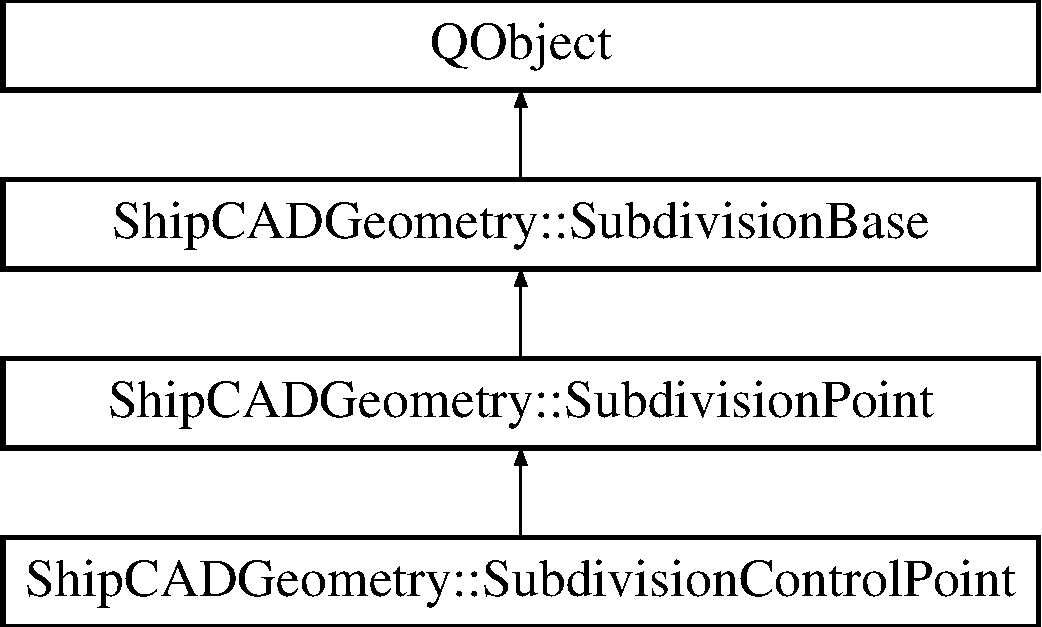
\includegraphics[height=4.000000cm]{classShipCADGeometry_1_1SubdivisionPoint}
\end{center}
\end{figure}
\subsection*{Public Types}
\begin{DoxyCompactItemize}
\item 
enum \hyperlink{classShipCADGeometry_1_1SubdivisionPoint_a03df9289cd8543cd3a567fa6c8e44c43}{vertex\-\_\-type\-\_\-t} \{ \hyperlink{classShipCADGeometry_1_1SubdivisionPoint_a03df9289cd8543cd3a567fa6c8e44c43a30dab596d2a968d283f161c490768ab0}{sv\-Regular} =0, 
\hyperlink{classShipCADGeometry_1_1SubdivisionPoint_a03df9289cd8543cd3a567fa6c8e44c43a7724ab9a0642a0ad21a896fb61a38035}{sv\-Crease}, 
\hyperlink{classShipCADGeometry_1_1SubdivisionPoint_a03df9289cd8543cd3a567fa6c8e44c43a94b87414422f77b76ecdbfadf29b985c}{sv\-Dart}, 
\hyperlink{classShipCADGeometry_1_1SubdivisionPoint_a03df9289cd8543cd3a567fa6c8e44c43adaf8032ead1bd79e03cff882b7b3987f}{sv\-Corner}
 \}
\end{DoxyCompactItemize}
\subsection*{Public Member Functions}
\begin{DoxyCompactItemize}
\item 
\hyperlink{classShipCADGeometry_1_1SubdivisionPoint_aed60af1f2fcbc89bad438a6a131a9f52}{Subdivision\-Point} (\hyperlink{classShipCADGeometry_1_1SubdivisionSurface}{Subdivision\-Surface} $\ast$owner)
\begin{DoxyCompactList}\small\item\em Constructor. \end{DoxyCompactList}\item 
virtual \hyperlink{classShipCADGeometry_1_1SubdivisionPoint_a218f451cd47873d61a4a987ec0cb3e6a}{$\sim$\-Subdivision\-Point} ()
\item 
virtual void \hyperlink{classShipCADGeometry_1_1SubdivisionPoint_aef22d2b6cb48e57ce69652eeb7a69711}{clear} ()
\begin{DoxyCompactList}\small\item\em Reset contents of the Point to default values. \end{DoxyCompactList}\item 
void \hyperlink{classShipCADGeometry_1_1SubdivisionPoint_acd07a93927bf7b6bfe9b4a3233efffdf}{add\-Edge} (\hyperlink{classShipCADGeometry_1_1SubdivisionEdge}{Subdivision\-Edge} $\ast$edge)
\begin{DoxyCompactList}\small\item\em add an Edge \end{DoxyCompactList}\item 
void \hyperlink{classShipCADGeometry_1_1SubdivisionPoint_a077ca16509feb6db73fa40a0098b72b4}{add\-Face} (\hyperlink{classShipCADGeometry_1_1SubdivisionFace}{Subdivision\-Face} $\ast$face)
\begin{DoxyCompactList}\small\item\em add a Face \end{DoxyCompactList}\item 
void \hyperlink{classShipCADGeometry_1_1SubdivisionPoint_a5c1e66b5a28923dca99fe856ce1dff0c}{delete\-Edge} (\hyperlink{classShipCADGeometry_1_1SubdivisionEdge}{Subdivision\-Edge} $\ast$edge)
\begin{DoxyCompactList}\small\item\em delete an Edge \end{DoxyCompactList}\item 
void \hyperlink{classShipCADGeometry_1_1SubdivisionPoint_a7ed94fd26e20c2e30d1f36be6b1a9b29}{delete\-Face} (\hyperlink{classShipCADGeometry_1_1SubdivisionFace}{Subdivision\-Face} $\ast$face)
\begin{DoxyCompactList}\small\item\em delete a Face \end{DoxyCompactList}\item 
void \hyperlink{classShipCADGeometry_1_1SubdivisionPoint_a63d20b811bb4af05b5f06014efd9385b}{destroy} ()
\item 
float \hyperlink{classShipCADGeometry_1_1SubdivisionPoint_aa07a859d70f97e57fc5318fc64a9d897}{get\-Curvature} ()
\begin{DoxyCompactList}\small\item\em find the curvature of the surface at this point \end{DoxyCompactList}\item 
Q\-Vector3\-D \hyperlink{classShipCADGeometry_1_1SubdivisionPoint_a0c9e47af796dacd9542d065bbd0d0fcf}{averaging} ()
\begin{DoxyCompactList}\small\item\em find the 3\-D coordinates of a point \end{DoxyCompactList}\item 
\hyperlink{classShipCADGeometry_1_1SubdivisionPoint}{Subdivision\-Point} $\ast$ \hyperlink{classShipCADGeometry_1_1SubdivisionPoint_a92632ddbe28fb6901e445b60eab8d3ee}{calculate\-Vertex\-Point} ()
\begin{DoxyCompactList}\small\item\em Create a vertex point. \end{DoxyCompactList}\item 
\hyperlink{classShipCADGeometry_1_1SubdivisionPoint_a03df9289cd8543cd3a567fa6c8e44c43}{vertex\-\_\-type\-\_\-t} \hyperlink{classShipCADGeometry_1_1SubdivisionPoint_a42fed467d1f925a9b8b6c46599cf81f4}{from\-Int} (int val)
\begin{DoxyCompactList}\small\item\em gets a vertex\-\_\-type\-\_\-t from integer \end{DoxyCompactList}\item 
Q\-Vector3\-D \hyperlink{classShipCADGeometry_1_1SubdivisionPoint_a0cf49d3e181eb00c08119721b33275bc}{get\-Coordinate} ()
\item 
virtual void \hyperlink{classShipCADGeometry_1_1SubdivisionPoint_a98ab99a0ccc4709a40e05b36147c0f55}{set\-Coordinate} (const Q\-Vector3\-D \&val)
\item 
Q\-Vector3\-D \hyperlink{classShipCADGeometry_1_1SubdivisionPoint_a8dd5facd4006480baea4a7f4487094f5}{get\-Normal} ()
\begin{DoxyCompactList}\small\item\em Calculate normal vector. \end{DoxyCompactList}\item 
\hyperlink{classShipCADGeometry_1_1SubdivisionFace}{Subdivision\-Face} $\ast$ \hyperlink{classShipCADGeometry_1_1SubdivisionPoint_a673d2a2c94f52e5523a012959417dcc3}{get\-Face} (size\-\_\-t index)
\item 
\hyperlink{classShipCADGeometry_1_1SubdivisionEdge}{Subdivision\-Edge} $\ast$ \hyperlink{classShipCADGeometry_1_1SubdivisionPoint_a518c4e3dc5de74950c87ff0f733716ba}{get\-Edge} (size\-\_\-t index)
\item 
bool \hyperlink{classShipCADGeometry_1_1SubdivisionPoint_afbcf1244015a92be04faed20163699f7}{is\-Boundary\-Vertex} ()
\item 
virtual size\-\_\-t \hyperlink{classShipCADGeometry_1_1SubdivisionPoint_a8406682549c10ec9e1a184132f6ed2f0}{get\-Index} ()
\begin{DoxyCompactList}\small\item\em index of this point in parent surface \end{DoxyCompactList}\item 
size\-\_\-t \hyperlink{classShipCADGeometry_1_1SubdivisionPoint_a7f798acd30dd4f5c9d0a9832ddd088de}{number\-Of\-Edges} ()
\item 
size\-\_\-t \hyperlink{classShipCADGeometry_1_1SubdivisionPoint_a24915c41e00cd2781aa40b09c7425486}{number\-Of\-Faces} ()
\item 
size\-\_\-t \hyperlink{classShipCADGeometry_1_1SubdivisionPoint_afc9659ec83083e7725ce14a12a74d2f0}{number\-Of\-Curves} ()
\item 
bool \hyperlink{classShipCADGeometry_1_1SubdivisionPoint_a6a0b4b628563cda2b2979ce6222e8a20}{is\-Regular\-Point} ()
\item 
Q\-Vector3\-D \hyperlink{classShipCADGeometry_1_1SubdivisionPoint_a0eb743069fe2ee2e99cdf7417b2400d5}{get\-Limit\-Point} ()
\item 
bool \hyperlink{classShipCADGeometry_1_1SubdivisionPoint_a88243019864c79766266cee627671183}{is\-Regular\-N\-U\-R\-B\-S\-Point} (std\-::vector$<$ \hyperlink{classShipCADGeometry_1_1SubdivisionFace}{Subdivision\-Face} $\ast$ $>$ \&faces)
\item 
size\-\_\-t \hyperlink{classShipCADGeometry_1_1SubdivisionPoint_a354475f80700fee46dcb46f8602c5345}{index\-Of\-Face} (\hyperlink{classShipCADGeometry_1_1SubdivisionFace}{Subdivision\-Face} $\ast$face)
\item 
bool \hyperlink{classShipCADGeometry_1_1SubdivisionPoint_ada0d082be616958c024bb1743d392e2f}{has\-Edge} (\hyperlink{classShipCADGeometry_1_1SubdivisionEdge}{Subdivision\-Edge} $\ast$edge)
\item 
bool \hyperlink{classShipCADGeometry_1_1SubdivisionPoint_a720d2fc986ba8a365e8722e0e3e28be5}{has\-Face} (\hyperlink{classShipCADGeometry_1_1SubdivisionFace}{Subdivision\-Face} $\ast$face)
\item 
\hyperlink{classShipCADGeometry_1_1SubdivisionPoint_a03df9289cd8543cd3a567fa6c8e44c43}{vertex\-\_\-type\-\_\-t} \hyperlink{classShipCADGeometry_1_1SubdivisionPoint_aca81609903ccd333db7f6f5f48d569ed}{get\-Vertex\-Type} ()
\item 
void \hyperlink{classShipCADGeometry_1_1SubdivisionPoint_a21d0f7b28fb19cb9f8d905c5f6eb9110}{set\-Vertex\-Type} (\hyperlink{classShipCADGeometry_1_1SubdivisionPoint_a03df9289cd8543cd3a567fa6c8e44c43}{vertex\-\_\-type\-\_\-t} nt)
\item 
virtual void \hyperlink{classShipCADGeometry_1_1SubdivisionPoint_aed72cf5e8dc67e980010d195f3a376a3}{dump} (std\-::ostream \&os, const char $\ast$prefix=\char`\"{}\char`\"{}) const 
\begin{DoxyCompactList}\small\item\em print out the element to a stream \end{DoxyCompactList}\end{DoxyCompactItemize}
\subsection*{Static Public Member Functions}
\begin{DoxyCompactItemize}
\item 
static \hyperlink{classShipCADGeometry_1_1SubdivisionPoint}{Subdivision\-Point} $\ast$ \hyperlink{classShipCADGeometry_1_1SubdivisionPoint_a8e907cca747b0483374d4fdde8eb4ad1}{construct} (\hyperlink{classShipCADGeometry_1_1SubdivisionSurface}{Subdivision\-Surface} $\ast$owner)
\begin{DoxyCompactList}\small\item\em make a point \end{DoxyCompactList}\end{DoxyCompactItemize}
\subsection*{Protected Member Functions}
\begin{DoxyCompactItemize}
\item 
void \hyperlink{classShipCADGeometry_1_1SubdivisionPoint_aa2d85a086268f335eefeaef0b48a96a1}{priv\-\_\-dump} (std\-::ostream \&os, const char $\ast$prefix) const 
\item 
float \hyperlink{classShipCADGeometry_1_1SubdivisionPoint_a72061d495903d8265f33bada30a0c416}{Angle\-\_\-\-V\-V\-\_\-3\-D} (const Q\-Vector3\-D \&p1, const Q\-Vector3\-D \&p2, const Q\-Vector3\-D \&p3)
\end{DoxyCompactItemize}
\subsection*{Protected Attributes}
\begin{DoxyCompactItemize}
\item 
std\-::vector$<$ \hyperlink{classShipCADGeometry_1_1SubdivisionFace}{Subdivision\-Face} $\ast$ $>$ \hyperlink{classShipCADGeometry_1_1SubdivisionPoint_aa6e398141f2b296763548ecdf904d200}{\-\_\-faces}
\item 
std\-::vector$<$ \hyperlink{classShipCADGeometry_1_1SubdivisionEdge}{Subdivision\-Edge} $\ast$ $>$ \hyperlink{classShipCADGeometry_1_1SubdivisionPoint_a1ee85e0a7815d8d737dcd6f654bf15a5}{\-\_\-edges}
\item 
Q\-Vector3\-D \hyperlink{classShipCADGeometry_1_1SubdivisionPoint_a7150fdf34fce9bc242b2266313c1c313}{\-\_\-coordinate}
\item 
\hyperlink{classShipCADGeometry_1_1SubdivisionPoint_a03df9289cd8543cd3a567fa6c8e44c43}{vertex\-\_\-type\-\_\-t} \hyperlink{classShipCADGeometry_1_1SubdivisionPoint_a9ffc795a56a1b963ba29725be17be266}{\-\_\-vtype}
\end{DoxyCompactItemize}
\subsection*{Properties}
\begin{DoxyCompactItemize}
\item 
Q\-Vector3\-D \hyperlink{classShipCADGeometry_1_1SubdivisionPoint_a4a8b002061482e596fb9228a8968cd57}{Coordinate}
\item 
float \hyperlink{classShipCADGeometry_1_1SubdivisionPoint_a7ca022ae7a31b478234ee212a24e3047}{Curvature}
\item 
bool \hyperlink{classShipCADGeometry_1_1SubdivisionPoint_af9d5dfd7c9c8bea01aab36388f0f0afe}{Is\-Boundary\-Vertex}
\item 
Q\-Vector3\-D \hyperlink{classShipCADGeometry_1_1SubdivisionPoint_a547c0cb9b9641fcb9d6a5beb3a86d59c}{Normal}
\item 
size\-\_\-t \hyperlink{classShipCADGeometry_1_1SubdivisionPoint_a3603dcd95c922b3852e0ba6f95a08b7f}{Vertex\-Index}
\item 
\hyperlink{classShipCADGeometry_1_1SubdivisionPoint_a03df9289cd8543cd3a567fa6c8e44c43}{vertex\-\_\-type\-\_\-t} \hyperlink{classShipCADGeometry_1_1SubdivisionPoint_a194e5f0d73d3af0bd21fa3cd4fa03296}{Vertex\-Type}
\end{DoxyCompactItemize}


\subsection{Detailed Description}
3\-D Point 

Used on boundaries of Faces. 

Definition at line 57 of file subdivpoint.\-h.



\subsection{Member Enumeration Documentation}
\hypertarget{classShipCADGeometry_1_1SubdivisionPoint_a03df9289cd8543cd3a567fa6c8e44c43}{\index{Ship\-C\-A\-D\-Geometry\-::\-Subdivision\-Point@{Ship\-C\-A\-D\-Geometry\-::\-Subdivision\-Point}!vertex\-\_\-type\-\_\-t@{vertex\-\_\-type\-\_\-t}}
\index{vertex\-\_\-type\-\_\-t@{vertex\-\_\-type\-\_\-t}!ShipCADGeometry::SubdivisionPoint@{Ship\-C\-A\-D\-Geometry\-::\-Subdivision\-Point}}
\subsubsection[{vertex\-\_\-type\-\_\-t}]{\setlength{\rightskip}{0pt plus 5cm}enum {\bf Ship\-C\-A\-D\-Geometry\-::\-Subdivision\-Point\-::vertex\-\_\-type\-\_\-t}}}\label{classShipCADGeometry_1_1SubdivisionPoint_a03df9289cd8543cd3a567fa6c8e44c43}
\begin{Desc}
\item[Enumerator]\par
\begin{description}
\index{sv\-Regular@{sv\-Regular}!Ship\-C\-A\-D\-Geometry\-::\-Subdivision\-Point@{Ship\-C\-A\-D\-Geometry\-::\-Subdivision\-Point}}\index{Ship\-C\-A\-D\-Geometry\-::\-Subdivision\-Point@{Ship\-C\-A\-D\-Geometry\-::\-Subdivision\-Point}!sv\-Regular@{sv\-Regular}}\item[{\em 
\hypertarget{classShipCADGeometry_1_1SubdivisionPoint_a03df9289cd8543cd3a567fa6c8e44c43a30dab596d2a968d283f161c490768ab0}{sv\-Regular}\label{classShipCADGeometry_1_1SubdivisionPoint_a03df9289cd8543cd3a567fa6c8e44c43a30dab596d2a968d283f161c490768ab0}
}]a regular point, no crease edges \index{sv\-Crease@{sv\-Crease}!Ship\-C\-A\-D\-Geometry\-::\-Subdivision\-Point@{Ship\-C\-A\-D\-Geometry\-::\-Subdivision\-Point}}\index{Ship\-C\-A\-D\-Geometry\-::\-Subdivision\-Point@{Ship\-C\-A\-D\-Geometry\-::\-Subdivision\-Point}!sv\-Crease@{sv\-Crease}}\item[{\em 
\hypertarget{classShipCADGeometry_1_1SubdivisionPoint_a03df9289cd8543cd3a567fa6c8e44c43a7724ab9a0642a0ad21a896fb61a38035}{sv\-Crease}\label{classShipCADGeometry_1_1SubdivisionPoint_a03df9289cd8543cd3a567fa6c8e44c43a7724ab9a0642a0ad21a896fb61a38035}
}]crease point, exactly 2 crease edges \index{sv\-Dart@{sv\-Dart}!Ship\-C\-A\-D\-Geometry\-::\-Subdivision\-Point@{Ship\-C\-A\-D\-Geometry\-::\-Subdivision\-Point}}\index{Ship\-C\-A\-D\-Geometry\-::\-Subdivision\-Point@{Ship\-C\-A\-D\-Geometry\-::\-Subdivision\-Point}!sv\-Dart@{sv\-Dart}}\item[{\em 
\hypertarget{classShipCADGeometry_1_1SubdivisionPoint_a03df9289cd8543cd3a567fa6c8e44c43a94b87414422f77b76ecdbfadf29b985c}{sv\-Dart}\label{classShipCADGeometry_1_1SubdivisionPoint_a03df9289cd8543cd3a567fa6c8e44c43a94b87414422f77b76ecdbfadf29b985c}
}]dart point, exactly 1 crease edge \index{sv\-Corner@{sv\-Corner}!Ship\-C\-A\-D\-Geometry\-::\-Subdivision\-Point@{Ship\-C\-A\-D\-Geometry\-::\-Subdivision\-Point}}\index{Ship\-C\-A\-D\-Geometry\-::\-Subdivision\-Point@{Ship\-C\-A\-D\-Geometry\-::\-Subdivision\-Point}!sv\-Corner@{sv\-Corner}}\item[{\em 
\hypertarget{classShipCADGeometry_1_1SubdivisionPoint_a03df9289cd8543cd3a567fa6c8e44c43adaf8032ead1bd79e03cff882b7b3987f}{sv\-Corner}\label{classShipCADGeometry_1_1SubdivisionPoint_a03df9289cd8543cd3a567fa6c8e44c43adaf8032ead1bd79e03cff882b7b3987f}
}]corner point that has more than 2 crease edges \end{description}
\end{Desc}


Definition at line 69 of file subdivpoint.\-h.



\subsection{Constructor \& Destructor Documentation}
\hypertarget{classShipCADGeometry_1_1SubdivisionPoint_aed60af1f2fcbc89bad438a6a131a9f52}{\index{Ship\-C\-A\-D\-Geometry\-::\-Subdivision\-Point@{Ship\-C\-A\-D\-Geometry\-::\-Subdivision\-Point}!Subdivision\-Point@{Subdivision\-Point}}
\index{Subdivision\-Point@{Subdivision\-Point}!ShipCADGeometry::SubdivisionPoint@{Ship\-C\-A\-D\-Geometry\-::\-Subdivision\-Point}}
\subsubsection[{Subdivision\-Point}]{\setlength{\rightskip}{0pt plus 5cm}Subdivision\-Point\-::\-Subdivision\-Point (
\begin{DoxyParamCaption}
\item[{{\bf Subdivision\-Surface} $\ast$}]{owner}
\end{DoxyParamCaption}
)\hspace{0.3cm}{\ttfamily [explicit]}}}\label{classShipCADGeometry_1_1SubdivisionPoint_aed60af1f2fcbc89bad438a6a131a9f52}


Constructor. 

Use the static construct method to create points 

Definition at line 65 of file subdivpoint.\-cpp.

\hypertarget{classShipCADGeometry_1_1SubdivisionPoint_a218f451cd47873d61a4a987ec0cb3e6a}{\index{Ship\-C\-A\-D\-Geometry\-::\-Subdivision\-Point@{Ship\-C\-A\-D\-Geometry\-::\-Subdivision\-Point}!$\sim$\-Subdivision\-Point@{$\sim$\-Subdivision\-Point}}
\index{$\sim$\-Subdivision\-Point@{$\sim$\-Subdivision\-Point}!ShipCADGeometry::SubdivisionPoint@{Ship\-C\-A\-D\-Geometry\-::\-Subdivision\-Point}}
\subsubsection[{$\sim$\-Subdivision\-Point}]{\setlength{\rightskip}{0pt plus 5cm}Subdivision\-Point\-::$\sim$\-Subdivision\-Point (
\begin{DoxyParamCaption}
{}
\end{DoxyParamCaption}
)\hspace{0.3cm}{\ttfamily [virtual]}}}\label{classShipCADGeometry_1_1SubdivisionPoint_a218f451cd47873d61a4a987ec0cb3e6a}


Definition at line 71 of file subdivpoint.\-cpp.



\subsection{Member Function Documentation}
\hypertarget{classShipCADGeometry_1_1SubdivisionPoint_acd07a93927bf7b6bfe9b4a3233efffdf}{\index{Ship\-C\-A\-D\-Geometry\-::\-Subdivision\-Point@{Ship\-C\-A\-D\-Geometry\-::\-Subdivision\-Point}!add\-Edge@{add\-Edge}}
\index{add\-Edge@{add\-Edge}!ShipCADGeometry::SubdivisionPoint@{Ship\-C\-A\-D\-Geometry\-::\-Subdivision\-Point}}
\subsubsection[{add\-Edge}]{\setlength{\rightskip}{0pt plus 5cm}void Subdivision\-Point\-::add\-Edge (
\begin{DoxyParamCaption}
\item[{{\bf Subdivision\-Edge} $\ast$}]{edge}
\end{DoxyParamCaption}
)}}\label{classShipCADGeometry_1_1SubdivisionPoint_acd07a93927bf7b6bfe9b4a3233efffdf}


add an Edge 


\begin{DoxyParams}{Parameters}
{\em edge} & the edge to add to this point \\
\hline
\end{DoxyParams}


Definition at line 304 of file subdivpoint.\-cpp.

\hypertarget{classShipCADGeometry_1_1SubdivisionPoint_a077ca16509feb6db73fa40a0098b72b4}{\index{Ship\-C\-A\-D\-Geometry\-::\-Subdivision\-Point@{Ship\-C\-A\-D\-Geometry\-::\-Subdivision\-Point}!add\-Face@{add\-Face}}
\index{add\-Face@{add\-Face}!ShipCADGeometry::SubdivisionPoint@{Ship\-C\-A\-D\-Geometry\-::\-Subdivision\-Point}}
\subsubsection[{add\-Face}]{\setlength{\rightskip}{0pt plus 5cm}void Subdivision\-Point\-::add\-Face (
\begin{DoxyParamCaption}
\item[{{\bf Subdivision\-Face} $\ast$}]{face}
\end{DoxyParamCaption}
)}}\label{classShipCADGeometry_1_1SubdivisionPoint_a077ca16509feb6db73fa40a0098b72b4}


add a Face 


\begin{DoxyParams}{Parameters}
{\em face} & the face to add to this point \\
\hline
\end{DoxyParams}


Definition at line 310 of file subdivpoint.\-cpp.

\hypertarget{classShipCADGeometry_1_1SubdivisionPoint_a72061d495903d8265f33bada30a0c416}{\index{Ship\-C\-A\-D\-Geometry\-::\-Subdivision\-Point@{Ship\-C\-A\-D\-Geometry\-::\-Subdivision\-Point}!Angle\-\_\-\-V\-V\-\_\-3\-D@{Angle\-\_\-\-V\-V\-\_\-3\-D}}
\index{Angle\-\_\-\-V\-V\-\_\-3\-D@{Angle\-\_\-\-V\-V\-\_\-3\-D}!ShipCADGeometry::SubdivisionPoint@{Ship\-C\-A\-D\-Geometry\-::\-Subdivision\-Point}}
\subsubsection[{Angle\-\_\-\-V\-V\-\_\-3\-D}]{\setlength{\rightskip}{0pt plus 5cm}float Subdivision\-Point\-::\-Angle\-\_\-\-V\-V\-\_\-3\-D (
\begin{DoxyParamCaption}
\item[{const Q\-Vector3\-D \&}]{p1, }
\item[{const Q\-Vector3\-D \&}]{p2, }
\item[{const Q\-Vector3\-D \&}]{p3}
\end{DoxyParamCaption}
)\hspace{0.3cm}{\ttfamily [protected]}}}\label{classShipCADGeometry_1_1SubdivisionPoint_a72061d495903d8265f33bada30a0c416}


Definition at line 121 of file subdivpoint.\-cpp.

\hypertarget{classShipCADGeometry_1_1SubdivisionPoint_a0c9e47af796dacd9542d065bbd0d0fcf}{\index{Ship\-C\-A\-D\-Geometry\-::\-Subdivision\-Point@{Ship\-C\-A\-D\-Geometry\-::\-Subdivision\-Point}!averaging@{averaging}}
\index{averaging@{averaging}!ShipCADGeometry::SubdivisionPoint@{Ship\-C\-A\-D\-Geometry\-::\-Subdivision\-Point}}
\subsubsection[{averaging}]{\setlength{\rightskip}{0pt plus 5cm}Q\-Vector3\-D Subdivision\-Point\-::averaging (
\begin{DoxyParamCaption}
{}
\end{DoxyParamCaption}
)}}\label{classShipCADGeometry_1_1SubdivisionPoint_a0c9e47af796dacd9542d065bbd0d0fcf}


find the 3\-D coordinates of a point 

Get coordinates for this point from faces and edges attached to this point If this is a crease point, then take all opposite end points of edges If this is not a crease point, but all other kinds, then take all points on faces attached to this point, weight them and calculate an average

\begin{DoxyReturn}{Returns}
coordinates of the calculated point 
\end{DoxyReturn}


Definition at line 316 of file subdivpoint.\-cpp.

\hypertarget{classShipCADGeometry_1_1SubdivisionPoint_a92632ddbe28fb6901e445b60eab8d3ee}{\index{Ship\-C\-A\-D\-Geometry\-::\-Subdivision\-Point@{Ship\-C\-A\-D\-Geometry\-::\-Subdivision\-Point}!calculate\-Vertex\-Point@{calculate\-Vertex\-Point}}
\index{calculate\-Vertex\-Point@{calculate\-Vertex\-Point}!ShipCADGeometry::SubdivisionPoint@{Ship\-C\-A\-D\-Geometry\-::\-Subdivision\-Point}}
\subsubsection[{calculate\-Vertex\-Point}]{\setlength{\rightskip}{0pt plus 5cm}{\bf Subdivision\-Point} $\ast$ Subdivision\-Point\-::calculate\-Vertex\-Point (
\begin{DoxyParamCaption}
{}
\end{DoxyParamCaption}
)}}\label{classShipCADGeometry_1_1SubdivisionPoint_a92632ddbe28fb6901e445b60eab8d3ee}


Create a vertex point. 

During the subdivision process, new points are created at the same position as existing points. This method creates a new point at the same position as the old one, also replaces the original point in any curves that contain it with the newly constructed point

\begin{DoxyReturn}{Returns}
new point that is a copy of this one 
\end{DoxyReturn}


Definition at line 399 of file subdivpoint.\-cpp.

\hypertarget{classShipCADGeometry_1_1SubdivisionPoint_aef22d2b6cb48e57ce69652eeb7a69711}{\index{Ship\-C\-A\-D\-Geometry\-::\-Subdivision\-Point@{Ship\-C\-A\-D\-Geometry\-::\-Subdivision\-Point}!clear@{clear}}
\index{clear@{clear}!ShipCADGeometry::SubdivisionPoint@{Ship\-C\-A\-D\-Geometry\-::\-Subdivision\-Point}}
\subsubsection[{clear}]{\setlength{\rightskip}{0pt plus 5cm}void Subdivision\-Point\-::clear (
\begin{DoxyParamCaption}
{}
\end{DoxyParamCaption}
)\hspace{0.3cm}{\ttfamily [virtual]}}}\label{classShipCADGeometry_1_1SubdivisionPoint_aef22d2b6cb48e57ce69652eeb7a69711}


Reset contents of the Point to default values. 



Implements \hyperlink{classShipCADGeometry_1_1SubdivisionBase_ae668920d97c0810c72996a531e0ca107}{Ship\-C\-A\-D\-Geometry\-::\-Subdivision\-Base}.



Definition at line 76 of file subdivpoint.\-cpp.

\hypertarget{classShipCADGeometry_1_1SubdivisionPoint_a8e907cca747b0483374d4fdde8eb4ad1}{\index{Ship\-C\-A\-D\-Geometry\-::\-Subdivision\-Point@{Ship\-C\-A\-D\-Geometry\-::\-Subdivision\-Point}!construct@{construct}}
\index{construct@{construct}!ShipCADGeometry::SubdivisionPoint@{Ship\-C\-A\-D\-Geometry\-::\-Subdivision\-Point}}
\subsubsection[{construct}]{\setlength{\rightskip}{0pt plus 5cm}{\bf Subdivision\-Point} $\ast$ Subdivision\-Point\-::construct (
\begin{DoxyParamCaption}
\item[{{\bf Subdivision\-Surface} $\ast$}]{owner}
\end{DoxyParamCaption}
)\hspace{0.3cm}{\ttfamily [static]}}}\label{classShipCADGeometry_1_1SubdivisionPoint_a8e907cca747b0483374d4fdde8eb4ad1}


make a point 

This doesn't add the point to the parent surface


\begin{DoxyParams}{Parameters}
{\em owner} & surface this point belongs to \\
\hline
\end{DoxyParams}


Definition at line 57 of file subdivpoint.\-cpp.

\hypertarget{classShipCADGeometry_1_1SubdivisionPoint_a5c1e66b5a28923dca99fe856ce1dff0c}{\index{Ship\-C\-A\-D\-Geometry\-::\-Subdivision\-Point@{Ship\-C\-A\-D\-Geometry\-::\-Subdivision\-Point}!delete\-Edge@{delete\-Edge}}
\index{delete\-Edge@{delete\-Edge}!ShipCADGeometry::SubdivisionPoint@{Ship\-C\-A\-D\-Geometry\-::\-Subdivision\-Point}}
\subsubsection[{delete\-Edge}]{\setlength{\rightskip}{0pt plus 5cm}void Subdivision\-Point\-::delete\-Edge (
\begin{DoxyParamCaption}
\item[{{\bf Subdivision\-Edge} $\ast$}]{edge}
\end{DoxyParamCaption}
)}}\label{classShipCADGeometry_1_1SubdivisionPoint_a5c1e66b5a28923dca99fe856ce1dff0c}


delete an Edge 


\begin{DoxyParams}{Parameters}
{\em edge} & the edge to delete from this point \\
\hline
\end{DoxyParams}


Definition at line 412 of file subdivpoint.\-cpp.

\hypertarget{classShipCADGeometry_1_1SubdivisionPoint_a7ed94fd26e20c2e30d1f36be6b1a9b29}{\index{Ship\-C\-A\-D\-Geometry\-::\-Subdivision\-Point@{Ship\-C\-A\-D\-Geometry\-::\-Subdivision\-Point}!delete\-Face@{delete\-Face}}
\index{delete\-Face@{delete\-Face}!ShipCADGeometry::SubdivisionPoint@{Ship\-C\-A\-D\-Geometry\-::\-Subdivision\-Point}}
\subsubsection[{delete\-Face}]{\setlength{\rightskip}{0pt plus 5cm}void Subdivision\-Point\-::delete\-Face (
\begin{DoxyParamCaption}
\item[{{\bf Subdivision\-Face} $\ast$}]{face}
\end{DoxyParamCaption}
)}}\label{classShipCADGeometry_1_1SubdivisionPoint_a7ed94fd26e20c2e30d1f36be6b1a9b29}


delete a Face 


\begin{DoxyParams}{Parameters}
{\em face} & the face to delete from this point \\
\hline
\end{DoxyParams}


Definition at line 420 of file subdivpoint.\-cpp.

\hypertarget{classShipCADGeometry_1_1SubdivisionPoint_a63d20b811bb4af05b5f06014efd9385b}{\index{Ship\-C\-A\-D\-Geometry\-::\-Subdivision\-Point@{Ship\-C\-A\-D\-Geometry\-::\-Subdivision\-Point}!destroy@{destroy}}
\index{destroy@{destroy}!ShipCADGeometry::SubdivisionPoint@{Ship\-C\-A\-D\-Geometry\-::\-Subdivision\-Point}}
\subsubsection[{destroy}]{\setlength{\rightskip}{0pt plus 5cm}void Ship\-C\-A\-D\-Geometry\-::\-Subdivision\-Point\-::destroy (
\begin{DoxyParamCaption}
{}
\end{DoxyParamCaption}
)}}\label{classShipCADGeometry_1_1SubdivisionPoint_a63d20b811bb4af05b5f06014efd9385b}
\hypertarget{classShipCADGeometry_1_1SubdivisionPoint_aed72cf5e8dc67e980010d195f3a376a3}{\index{Ship\-C\-A\-D\-Geometry\-::\-Subdivision\-Point@{Ship\-C\-A\-D\-Geometry\-::\-Subdivision\-Point}!dump@{dump}}
\index{dump@{dump}!ShipCADGeometry::SubdivisionPoint@{Ship\-C\-A\-D\-Geometry\-::\-Subdivision\-Point}}
\subsubsection[{dump}]{\setlength{\rightskip}{0pt plus 5cm}void Subdivision\-Point\-::dump (
\begin{DoxyParamCaption}
\item[{std\-::ostream \&}]{os, }
\item[{const char $\ast$}]{prefix = {\ttfamily \char`\"{}\char`\"{}}}
\end{DoxyParamCaption}
) const\hspace{0.3cm}{\ttfamily [virtual]}}}\label{classShipCADGeometry_1_1SubdivisionPoint_aed72cf5e8dc67e980010d195f3a376a3}


print out the element to a stream 


\begin{DoxyParams}{Parameters}
{\em os} & the output stream \\
\hline
{\em prefix} & string to prefix on each line output \\
\hline
\end{DoxyParams}


Reimplemented from \hyperlink{classShipCADGeometry_1_1SubdivisionBase_a7807e64ac8d2acc3da572e03cf0523b6}{Ship\-C\-A\-D\-Geometry\-::\-Subdivision\-Base}.



Reimplemented in \hyperlink{classShipCADGeometry_1_1SubdivisionControlPoint_a4a9d6e45291c27f19f0d76c9b9d19048}{Ship\-C\-A\-D\-Geometry\-::\-Subdivision\-Control\-Point}.



Definition at line 476 of file subdivpoint.\-cpp.

\hypertarget{classShipCADGeometry_1_1SubdivisionPoint_a42fed467d1f925a9b8b6c46599cf81f4}{\index{Ship\-C\-A\-D\-Geometry\-::\-Subdivision\-Point@{Ship\-C\-A\-D\-Geometry\-::\-Subdivision\-Point}!from\-Int@{from\-Int}}
\index{from\-Int@{from\-Int}!ShipCADGeometry::SubdivisionPoint@{Ship\-C\-A\-D\-Geometry\-::\-Subdivision\-Point}}
\subsubsection[{from\-Int}]{\setlength{\rightskip}{0pt plus 5cm}{\bf Subdivision\-Point\-::vertex\-\_\-type\-\_\-t} Subdivision\-Point\-::from\-Int (
\begin{DoxyParamCaption}
\item[{int}]{val}
\end{DoxyParamCaption}
)}}\label{classShipCADGeometry_1_1SubdivisionPoint_a42fed467d1f925a9b8b6c46599cf81f4}


gets a vertex\-\_\-type\-\_\-t from integer 

Returns the vertex\-\_\-type\-\_\-t from an integer, used in serialization


\begin{DoxyParams}{Parameters}
{\em val} & an integer representing vertex type \\
\hline
\end{DoxyParams}
\begin{DoxyReturn}{Returns}
vertex type 
\end{DoxyReturn}


Definition at line 84 of file subdivpoint.\-cpp.

\hypertarget{classShipCADGeometry_1_1SubdivisionPoint_a0cf49d3e181eb00c08119721b33275bc}{\index{Ship\-C\-A\-D\-Geometry\-::\-Subdivision\-Point@{Ship\-C\-A\-D\-Geometry\-::\-Subdivision\-Point}!get\-Coordinate@{get\-Coordinate}}
\index{get\-Coordinate@{get\-Coordinate}!ShipCADGeometry::SubdivisionPoint@{Ship\-C\-A\-D\-Geometry\-::\-Subdivision\-Point}}
\subsubsection[{get\-Coordinate}]{\setlength{\rightskip}{0pt plus 5cm}Q\-Vector3\-D Subdivision\-Point\-::get\-Coordinate (
\begin{DoxyParamCaption}
{}
\end{DoxyParamCaption}
)}}\label{classShipCADGeometry_1_1SubdivisionPoint_a0cf49d3e181eb00c08119721b33275bc}


Definition at line 116 of file subdivpoint.\-cpp.

\hypertarget{classShipCADGeometry_1_1SubdivisionPoint_aa07a859d70f97e57fc5318fc64a9d897}{\index{Ship\-C\-A\-D\-Geometry\-::\-Subdivision\-Point@{Ship\-C\-A\-D\-Geometry\-::\-Subdivision\-Point}!get\-Curvature@{get\-Curvature}}
\index{get\-Curvature@{get\-Curvature}!ShipCADGeometry::SubdivisionPoint@{Ship\-C\-A\-D\-Geometry\-::\-Subdivision\-Point}}
\subsubsection[{get\-Curvature}]{\setlength{\rightskip}{0pt plus 5cm}float Subdivision\-Point\-::get\-Curvature (
\begin{DoxyParamCaption}
{}
\end{DoxyParamCaption}
)}}\label{classShipCADGeometry_1_1SubdivisionPoint_aa07a859d70f97e57fc5318fc64a9d897}


find the curvature of the surface at this point 

For each pair of points attached to faces attached to this point, take the dot product of the triangular face created from that pair and this point. Add these dot products together and convert from radians to degrees

\begin{DoxyReturn}{Returns}
the curvature of the surface at this point 
\end{DoxyReturn}


Definition at line 137 of file subdivpoint.\-cpp.

\hypertarget{classShipCADGeometry_1_1SubdivisionPoint_a518c4e3dc5de74950c87ff0f733716ba}{\index{Ship\-C\-A\-D\-Geometry\-::\-Subdivision\-Point@{Ship\-C\-A\-D\-Geometry\-::\-Subdivision\-Point}!get\-Edge@{get\-Edge}}
\index{get\-Edge@{get\-Edge}!ShipCADGeometry::SubdivisionPoint@{Ship\-C\-A\-D\-Geometry\-::\-Subdivision\-Point}}
\subsubsection[{get\-Edge}]{\setlength{\rightskip}{0pt plus 5cm}{\bf Subdivision\-Edge} $\ast$ Subdivision\-Point\-::get\-Edge (
\begin{DoxyParamCaption}
\item[{size\-\_\-t}]{index}
\end{DoxyParamCaption}
)}}\label{classShipCADGeometry_1_1SubdivisionPoint_a518c4e3dc5de74950c87ff0f733716ba}


Definition at line 97 of file subdivpoint.\-cpp.

\hypertarget{classShipCADGeometry_1_1SubdivisionPoint_a673d2a2c94f52e5523a012959417dcc3}{\index{Ship\-C\-A\-D\-Geometry\-::\-Subdivision\-Point@{Ship\-C\-A\-D\-Geometry\-::\-Subdivision\-Point}!get\-Face@{get\-Face}}
\index{get\-Face@{get\-Face}!ShipCADGeometry::SubdivisionPoint@{Ship\-C\-A\-D\-Geometry\-::\-Subdivision\-Point}}
\subsubsection[{get\-Face}]{\setlength{\rightskip}{0pt plus 5cm}{\bf Subdivision\-Face} $\ast$ Subdivision\-Point\-::get\-Face (
\begin{DoxyParamCaption}
\item[{size\-\_\-t}]{index}
\end{DoxyParamCaption}
)}}\label{classShipCADGeometry_1_1SubdivisionPoint_a673d2a2c94f52e5523a012959417dcc3}


Definition at line 104 of file subdivpoint.\-cpp.

\hypertarget{classShipCADGeometry_1_1SubdivisionPoint_a8406682549c10ec9e1a184132f6ed2f0}{\index{Ship\-C\-A\-D\-Geometry\-::\-Subdivision\-Point@{Ship\-C\-A\-D\-Geometry\-::\-Subdivision\-Point}!get\-Index@{get\-Index}}
\index{get\-Index@{get\-Index}!ShipCADGeometry::SubdivisionPoint@{Ship\-C\-A\-D\-Geometry\-::\-Subdivision\-Point}}
\subsubsection[{get\-Index}]{\setlength{\rightskip}{0pt plus 5cm}size\-\_\-t Subdivision\-Point\-::get\-Index (
\begin{DoxyParamCaption}
{}
\end{DoxyParamCaption}
)\hspace{0.3cm}{\ttfamily [virtual]}}}\label{classShipCADGeometry_1_1SubdivisionPoint_a8406682549c10ec9e1a184132f6ed2f0}


index of this point in parent surface 

\begin{DoxyReturn}{Returns}
the index of this point in parent surface 
\end{DoxyReturn}


Reimplemented in \hyperlink{classShipCADGeometry_1_1SubdivisionControlPoint_a13c569f0894ba6193a3abf894bc4b517}{Ship\-C\-A\-D\-Geometry\-::\-Subdivision\-Control\-Point}.



Definition at line 111 of file subdivpoint.\-cpp.

\hypertarget{classShipCADGeometry_1_1SubdivisionPoint_a0eb743069fe2ee2e99cdf7417b2400d5}{\index{Ship\-C\-A\-D\-Geometry\-::\-Subdivision\-Point@{Ship\-C\-A\-D\-Geometry\-::\-Subdivision\-Point}!get\-Limit\-Point@{get\-Limit\-Point}}
\index{get\-Limit\-Point@{get\-Limit\-Point}!ShipCADGeometry::SubdivisionPoint@{Ship\-C\-A\-D\-Geometry\-::\-Subdivision\-Point}}
\subsubsection[{get\-Limit\-Point}]{\setlength{\rightskip}{0pt plus 5cm}Q\-Vector3\-D Subdivision\-Point\-::get\-Limit\-Point (
\begin{DoxyParamCaption}
{}
\end{DoxyParamCaption}
)}}\label{classShipCADGeometry_1_1SubdivisionPoint_a0eb743069fe2ee2e99cdf7417b2400d5}


Definition at line 221 of file subdivpoint.\-cpp.

\hypertarget{classShipCADGeometry_1_1SubdivisionPoint_a8dd5facd4006480baea4a7f4487094f5}{\index{Ship\-C\-A\-D\-Geometry\-::\-Subdivision\-Point@{Ship\-C\-A\-D\-Geometry\-::\-Subdivision\-Point}!get\-Normal@{get\-Normal}}
\index{get\-Normal@{get\-Normal}!ShipCADGeometry::SubdivisionPoint@{Ship\-C\-A\-D\-Geometry\-::\-Subdivision\-Point}}
\subsubsection[{get\-Normal}]{\setlength{\rightskip}{0pt plus 5cm}Q\-Vector3\-D Subdivision\-Point\-::get\-Normal (
\begin{DoxyParamCaption}
{}
\end{DoxyParamCaption}
)}}\label{classShipCADGeometry_1_1SubdivisionPoint_a8dd5facd4006480baea4a7f4487094f5}


Calculate normal vector. 

Find the surface normal at this point by finding the normal of each face attached to this point, and adding them together.

\begin{DoxyReturn}{Returns}
coordinates of the normal vector 
\end{DoxyReturn}


Definition at line 446 of file subdivpoint.\-cpp.

\hypertarget{classShipCADGeometry_1_1SubdivisionPoint_aca81609903ccd333db7f6f5f48d569ed}{\index{Ship\-C\-A\-D\-Geometry\-::\-Subdivision\-Point@{Ship\-C\-A\-D\-Geometry\-::\-Subdivision\-Point}!get\-Vertex\-Type@{get\-Vertex\-Type}}
\index{get\-Vertex\-Type@{get\-Vertex\-Type}!ShipCADGeometry::SubdivisionPoint@{Ship\-C\-A\-D\-Geometry\-::\-Subdivision\-Point}}
\subsubsection[{get\-Vertex\-Type}]{\setlength{\rightskip}{0pt plus 5cm}{\bf vertex\-\_\-type\-\_\-t} Ship\-C\-A\-D\-Geometry\-::\-Subdivision\-Point\-::get\-Vertex\-Type (
\begin{DoxyParamCaption}
{}
\end{DoxyParamCaption}
)\hspace{0.3cm}{\ttfamily [inline]}}}\label{classShipCADGeometry_1_1SubdivisionPoint_aca81609903ccd333db7f6f5f48d569ed}


Definition at line 180 of file subdivpoint.\-h.

\hypertarget{classShipCADGeometry_1_1SubdivisionPoint_ada0d082be616958c024bb1743d392e2f}{\index{Ship\-C\-A\-D\-Geometry\-::\-Subdivision\-Point@{Ship\-C\-A\-D\-Geometry\-::\-Subdivision\-Point}!has\-Edge@{has\-Edge}}
\index{has\-Edge@{has\-Edge}!ShipCADGeometry::SubdivisionPoint@{Ship\-C\-A\-D\-Geometry\-::\-Subdivision\-Point}}
\subsubsection[{has\-Edge}]{\setlength{\rightskip}{0pt plus 5cm}bool Subdivision\-Point\-::has\-Edge (
\begin{DoxyParamCaption}
\item[{{\bf Subdivision\-Edge} $\ast$}]{edge}
\end{DoxyParamCaption}
)}}\label{classShipCADGeometry_1_1SubdivisionPoint_ada0d082be616958c024bb1743d392e2f}


Definition at line 436 of file subdivpoint.\-cpp.

\hypertarget{classShipCADGeometry_1_1SubdivisionPoint_a720d2fc986ba8a365e8722e0e3e28be5}{\index{Ship\-C\-A\-D\-Geometry\-::\-Subdivision\-Point@{Ship\-C\-A\-D\-Geometry\-::\-Subdivision\-Point}!has\-Face@{has\-Face}}
\index{has\-Face@{has\-Face}!ShipCADGeometry::SubdivisionPoint@{Ship\-C\-A\-D\-Geometry\-::\-Subdivision\-Point}}
\subsubsection[{has\-Face}]{\setlength{\rightskip}{0pt plus 5cm}bool Subdivision\-Point\-::has\-Face (
\begin{DoxyParamCaption}
\item[{{\bf Subdivision\-Face} $\ast$}]{face}
\end{DoxyParamCaption}
)}}\label{classShipCADGeometry_1_1SubdivisionPoint_a720d2fc986ba8a365e8722e0e3e28be5}


Definition at line 441 of file subdivpoint.\-cpp.

\hypertarget{classShipCADGeometry_1_1SubdivisionPoint_a354475f80700fee46dcb46f8602c5345}{\index{Ship\-C\-A\-D\-Geometry\-::\-Subdivision\-Point@{Ship\-C\-A\-D\-Geometry\-::\-Subdivision\-Point}!index\-Of\-Face@{index\-Of\-Face}}
\index{index\-Of\-Face@{index\-Of\-Face}!ShipCADGeometry::SubdivisionPoint@{Ship\-C\-A\-D\-Geometry\-::\-Subdivision\-Point}}
\subsubsection[{index\-Of\-Face}]{\setlength{\rightskip}{0pt plus 5cm}size\-\_\-t Subdivision\-Point\-::index\-Of\-Face (
\begin{DoxyParamCaption}
\item[{{\bf Subdivision\-Face} $\ast$}]{face}
\end{DoxyParamCaption}
)}}\label{classShipCADGeometry_1_1SubdivisionPoint_a354475f80700fee46dcb46f8602c5345}


Definition at line 428 of file subdivpoint.\-cpp.

\hypertarget{classShipCADGeometry_1_1SubdivisionPoint_afbcf1244015a92be04faed20163699f7}{\index{Ship\-C\-A\-D\-Geometry\-::\-Subdivision\-Point@{Ship\-C\-A\-D\-Geometry\-::\-Subdivision\-Point}!is\-Boundary\-Vertex@{is\-Boundary\-Vertex}}
\index{is\-Boundary\-Vertex@{is\-Boundary\-Vertex}!ShipCADGeometry::SubdivisionPoint@{Ship\-C\-A\-D\-Geometry\-::\-Subdivision\-Point}}
\subsubsection[{is\-Boundary\-Vertex}]{\setlength{\rightskip}{0pt plus 5cm}bool Subdivision\-Point\-::is\-Boundary\-Vertex (
\begin{DoxyParamCaption}
{}
\end{DoxyParamCaption}
)}}\label{classShipCADGeometry_1_1SubdivisionPoint_afbcf1244015a92be04faed20163699f7}


Definition at line 160 of file subdivpoint.\-cpp.

\hypertarget{classShipCADGeometry_1_1SubdivisionPoint_a88243019864c79766266cee627671183}{\index{Ship\-C\-A\-D\-Geometry\-::\-Subdivision\-Point@{Ship\-C\-A\-D\-Geometry\-::\-Subdivision\-Point}!is\-Regular\-N\-U\-R\-B\-S\-Point@{is\-Regular\-N\-U\-R\-B\-S\-Point}}
\index{is\-Regular\-N\-U\-R\-B\-S\-Point@{is\-Regular\-N\-U\-R\-B\-S\-Point}!ShipCADGeometry::SubdivisionPoint@{Ship\-C\-A\-D\-Geometry\-::\-Subdivision\-Point}}
\subsubsection[{is\-Regular\-N\-U\-R\-B\-S\-Point}]{\setlength{\rightskip}{0pt plus 5cm}bool Subdivision\-Point\-::is\-Regular\-N\-U\-R\-B\-S\-Point (
\begin{DoxyParamCaption}
\item[{std\-::vector$<$ {\bf Subdivision\-Face} $\ast$ $>$ \&}]{faces}
\end{DoxyParamCaption}
)}}\label{classShipCADGeometry_1_1SubdivisionPoint_a88243019864c79766266cee627671183}


Definition at line 268 of file subdivpoint.\-cpp.

\hypertarget{classShipCADGeometry_1_1SubdivisionPoint_a6a0b4b628563cda2b2979ce6222e8a20}{\index{Ship\-C\-A\-D\-Geometry\-::\-Subdivision\-Point@{Ship\-C\-A\-D\-Geometry\-::\-Subdivision\-Point}!is\-Regular\-Point@{is\-Regular\-Point}}
\index{is\-Regular\-Point@{is\-Regular\-Point}!ShipCADGeometry::SubdivisionPoint@{Ship\-C\-A\-D\-Geometry\-::\-Subdivision\-Point}}
\subsubsection[{is\-Regular\-Point}]{\setlength{\rightskip}{0pt plus 5cm}bool Subdivision\-Point\-::is\-Regular\-Point (
\begin{DoxyParamCaption}
{}
\end{DoxyParamCaption}
)}}\label{classShipCADGeometry_1_1SubdivisionPoint_a6a0b4b628563cda2b2979ce6222e8a20}


Definition at line 179 of file subdivpoint.\-cpp.

\hypertarget{classShipCADGeometry_1_1SubdivisionPoint_afc9659ec83083e7725ce14a12a74d2f0}{\index{Ship\-C\-A\-D\-Geometry\-::\-Subdivision\-Point@{Ship\-C\-A\-D\-Geometry\-::\-Subdivision\-Point}!number\-Of\-Curves@{number\-Of\-Curves}}
\index{number\-Of\-Curves@{number\-Of\-Curves}!ShipCADGeometry::SubdivisionPoint@{Ship\-C\-A\-D\-Geometry\-::\-Subdivision\-Point}}
\subsubsection[{number\-Of\-Curves}]{\setlength{\rightskip}{0pt plus 5cm}size\-\_\-t Subdivision\-Point\-::number\-Of\-Curves (
\begin{DoxyParamCaption}
{}
\end{DoxyParamCaption}
)}}\label{classShipCADGeometry_1_1SubdivisionPoint_afc9659ec83083e7725ce14a12a74d2f0}


Definition at line 170 of file subdivpoint.\-cpp.

\hypertarget{classShipCADGeometry_1_1SubdivisionPoint_a7f798acd30dd4f5c9d0a9832ddd088de}{\index{Ship\-C\-A\-D\-Geometry\-::\-Subdivision\-Point@{Ship\-C\-A\-D\-Geometry\-::\-Subdivision\-Point}!number\-Of\-Edges@{number\-Of\-Edges}}
\index{number\-Of\-Edges@{number\-Of\-Edges}!ShipCADGeometry::SubdivisionPoint@{Ship\-C\-A\-D\-Geometry\-::\-Subdivision\-Point}}
\subsubsection[{number\-Of\-Edges}]{\setlength{\rightskip}{0pt plus 5cm}size\-\_\-t Ship\-C\-A\-D\-Geometry\-::\-Subdivision\-Point\-::number\-Of\-Edges (
\begin{DoxyParamCaption}
{}
\end{DoxyParamCaption}
)\hspace{0.3cm}{\ttfamily [inline]}}}\label{classShipCADGeometry_1_1SubdivisionPoint_a7f798acd30dd4f5c9d0a9832ddd088de}


Definition at line 171 of file subdivpoint.\-h.

\hypertarget{classShipCADGeometry_1_1SubdivisionPoint_a24915c41e00cd2781aa40b09c7425486}{\index{Ship\-C\-A\-D\-Geometry\-::\-Subdivision\-Point@{Ship\-C\-A\-D\-Geometry\-::\-Subdivision\-Point}!number\-Of\-Faces@{number\-Of\-Faces}}
\index{number\-Of\-Faces@{number\-Of\-Faces}!ShipCADGeometry::SubdivisionPoint@{Ship\-C\-A\-D\-Geometry\-::\-Subdivision\-Point}}
\subsubsection[{number\-Of\-Faces}]{\setlength{\rightskip}{0pt plus 5cm}size\-\_\-t Ship\-C\-A\-D\-Geometry\-::\-Subdivision\-Point\-::number\-Of\-Faces (
\begin{DoxyParamCaption}
{}
\end{DoxyParamCaption}
)\hspace{0.3cm}{\ttfamily [inline]}}}\label{classShipCADGeometry_1_1SubdivisionPoint_a24915c41e00cd2781aa40b09c7425486}


Definition at line 172 of file subdivpoint.\-h.

\hypertarget{classShipCADGeometry_1_1SubdivisionPoint_aa2d85a086268f335eefeaef0b48a96a1}{\index{Ship\-C\-A\-D\-Geometry\-::\-Subdivision\-Point@{Ship\-C\-A\-D\-Geometry\-::\-Subdivision\-Point}!priv\-\_\-dump@{priv\-\_\-dump}}
\index{priv\-\_\-dump@{priv\-\_\-dump}!ShipCADGeometry::SubdivisionPoint@{Ship\-C\-A\-D\-Geometry\-::\-Subdivision\-Point}}
\subsubsection[{priv\-\_\-dump}]{\setlength{\rightskip}{0pt plus 5cm}void Subdivision\-Point\-::priv\-\_\-dump (
\begin{DoxyParamCaption}
\item[{std\-::ostream \&}]{os, }
\item[{const char $\ast$}]{prefix}
\end{DoxyParamCaption}
) const\hspace{0.3cm}{\ttfamily [protected]}}}\label{classShipCADGeometry_1_1SubdivisionPoint_aa2d85a086268f335eefeaef0b48a96a1}


Definition at line 484 of file subdivpoint.\-cpp.

\hypertarget{classShipCADGeometry_1_1SubdivisionPoint_a98ab99a0ccc4709a40e05b36147c0f55}{\index{Ship\-C\-A\-D\-Geometry\-::\-Subdivision\-Point@{Ship\-C\-A\-D\-Geometry\-::\-Subdivision\-Point}!set\-Coordinate@{set\-Coordinate}}
\index{set\-Coordinate@{set\-Coordinate}!ShipCADGeometry::SubdivisionPoint@{Ship\-C\-A\-D\-Geometry\-::\-Subdivision\-Point}}
\subsubsection[{set\-Coordinate}]{\setlength{\rightskip}{0pt plus 5cm}void Subdivision\-Point\-::set\-Coordinate (
\begin{DoxyParamCaption}
\item[{const Q\-Vector3\-D \&}]{val}
\end{DoxyParamCaption}
)\hspace{0.3cm}{\ttfamily [virtual]}}}\label{classShipCADGeometry_1_1SubdivisionPoint_a98ab99a0ccc4709a40e05b36147c0f55}


Reimplemented in \hyperlink{classShipCADGeometry_1_1SubdivisionControlPoint_a54a5233e02ef34a174c24d5dcf3c6407}{Ship\-C\-A\-D\-Geometry\-::\-Subdivision\-Control\-Point}.



Definition at line 299 of file subdivpoint.\-cpp.

\hypertarget{classShipCADGeometry_1_1SubdivisionPoint_a21d0f7b28fb19cb9f8d905c5f6eb9110}{\index{Ship\-C\-A\-D\-Geometry\-::\-Subdivision\-Point@{Ship\-C\-A\-D\-Geometry\-::\-Subdivision\-Point}!set\-Vertex\-Type@{set\-Vertex\-Type}}
\index{set\-Vertex\-Type@{set\-Vertex\-Type}!ShipCADGeometry::SubdivisionPoint@{Ship\-C\-A\-D\-Geometry\-::\-Subdivision\-Point}}
\subsubsection[{set\-Vertex\-Type}]{\setlength{\rightskip}{0pt plus 5cm}void Ship\-C\-A\-D\-Geometry\-::\-Subdivision\-Point\-::set\-Vertex\-Type (
\begin{DoxyParamCaption}
\item[{{\bf vertex\-\_\-type\-\_\-t}}]{nt}
\end{DoxyParamCaption}
)\hspace{0.3cm}{\ttfamily [inline]}}}\label{classShipCADGeometry_1_1SubdivisionPoint_a21d0f7b28fb19cb9f8d905c5f6eb9110}


Definition at line 181 of file subdivpoint.\-h.



\subsection{Member Data Documentation}
\hypertarget{classShipCADGeometry_1_1SubdivisionPoint_a7150fdf34fce9bc242b2266313c1c313}{\index{Ship\-C\-A\-D\-Geometry\-::\-Subdivision\-Point@{Ship\-C\-A\-D\-Geometry\-::\-Subdivision\-Point}!\-\_\-coordinate@{\-\_\-coordinate}}
\index{\-\_\-coordinate@{\-\_\-coordinate}!ShipCADGeometry::SubdivisionPoint@{Ship\-C\-A\-D\-Geometry\-::\-Subdivision\-Point}}
\subsubsection[{\-\_\-coordinate}]{\setlength{\rightskip}{0pt plus 5cm}Q\-Vector3\-D Ship\-C\-A\-D\-Geometry\-::\-Subdivision\-Point\-::\-\_\-coordinate\hspace{0.3cm}{\ttfamily [protected]}}}\label{classShipCADGeometry_1_1SubdivisionPoint_a7150fdf34fce9bc242b2266313c1c313}
3\-D coordinates of this point 

Definition at line 205 of file subdivpoint.\-h.

\hypertarget{classShipCADGeometry_1_1SubdivisionPoint_a1ee85e0a7815d8d737dcd6f654bf15a5}{\index{Ship\-C\-A\-D\-Geometry\-::\-Subdivision\-Point@{Ship\-C\-A\-D\-Geometry\-::\-Subdivision\-Point}!\-\_\-edges@{\-\_\-edges}}
\index{\-\_\-edges@{\-\_\-edges}!ShipCADGeometry::SubdivisionPoint@{Ship\-C\-A\-D\-Geometry\-::\-Subdivision\-Point}}
\subsubsection[{\-\_\-edges}]{\setlength{\rightskip}{0pt plus 5cm}std\-::vector$<${\bf Subdivision\-Edge}$\ast$$>$ Ship\-C\-A\-D\-Geometry\-::\-Subdivision\-Point\-::\-\_\-edges\hspace{0.3cm}{\ttfamily [protected]}}}\label{classShipCADGeometry_1_1SubdivisionPoint_a1ee85e0a7815d8d737dcd6f654bf15a5}
list of edges attached to this point 

Definition at line 204 of file subdivpoint.\-h.

\hypertarget{classShipCADGeometry_1_1SubdivisionPoint_aa6e398141f2b296763548ecdf904d200}{\index{Ship\-C\-A\-D\-Geometry\-::\-Subdivision\-Point@{Ship\-C\-A\-D\-Geometry\-::\-Subdivision\-Point}!\-\_\-faces@{\-\_\-faces}}
\index{\-\_\-faces@{\-\_\-faces}!ShipCADGeometry::SubdivisionPoint@{Ship\-C\-A\-D\-Geometry\-::\-Subdivision\-Point}}
\subsubsection[{\-\_\-faces}]{\setlength{\rightskip}{0pt plus 5cm}std\-::vector$<${\bf Subdivision\-Face}$\ast$$>$ Ship\-C\-A\-D\-Geometry\-::\-Subdivision\-Point\-::\-\_\-faces\hspace{0.3cm}{\ttfamily [protected]}}}\label{classShipCADGeometry_1_1SubdivisionPoint_aa6e398141f2b296763548ecdf904d200}
list of faces attached to this point 

Definition at line 203 of file subdivpoint.\-h.

\hypertarget{classShipCADGeometry_1_1SubdivisionPoint_a9ffc795a56a1b963ba29725be17be266}{\index{Ship\-C\-A\-D\-Geometry\-::\-Subdivision\-Point@{Ship\-C\-A\-D\-Geometry\-::\-Subdivision\-Point}!\-\_\-vtype@{\-\_\-vtype}}
\index{\-\_\-vtype@{\-\_\-vtype}!ShipCADGeometry::SubdivisionPoint@{Ship\-C\-A\-D\-Geometry\-::\-Subdivision\-Point}}
\subsubsection[{\-\_\-vtype}]{\setlength{\rightskip}{0pt plus 5cm}{\bf vertex\-\_\-type\-\_\-t} Ship\-C\-A\-D\-Geometry\-::\-Subdivision\-Point\-::\-\_\-vtype\hspace{0.3cm}{\ttfamily [protected]}}}\label{classShipCADGeometry_1_1SubdivisionPoint_a9ffc795a56a1b963ba29725be17be266}
vertex type of this point 

Definition at line 206 of file subdivpoint.\-h.



\subsection{Property Documentation}
\hypertarget{classShipCADGeometry_1_1SubdivisionPoint_a4a8b002061482e596fb9228a8968cd57}{\index{Ship\-C\-A\-D\-Geometry\-::\-Subdivision\-Point@{Ship\-C\-A\-D\-Geometry\-::\-Subdivision\-Point}!Coordinate@{Coordinate}}
\index{Coordinate@{Coordinate}!ShipCADGeometry::SubdivisionPoint@{Ship\-C\-A\-D\-Geometry\-::\-Subdivision\-Point}}
\subsubsection[{Coordinate}]{\setlength{\rightskip}{0pt plus 5cm}Q\-Vector3\-D Ship\-C\-A\-D\-Geometry\-::\-Subdivision\-Point\-::\-Coordinate\hspace{0.3cm}{\ttfamily [read]}, {\ttfamily [write]}}}\label{classShipCADGeometry_1_1SubdivisionPoint_a4a8b002061482e596fb9228a8968cd57}


Definition at line 60 of file subdivpoint.\-h.

\hypertarget{classShipCADGeometry_1_1SubdivisionPoint_a7ca022ae7a31b478234ee212a24e3047}{\index{Ship\-C\-A\-D\-Geometry\-::\-Subdivision\-Point@{Ship\-C\-A\-D\-Geometry\-::\-Subdivision\-Point}!Curvature@{Curvature}}
\index{Curvature@{Curvature}!ShipCADGeometry::SubdivisionPoint@{Ship\-C\-A\-D\-Geometry\-::\-Subdivision\-Point}}
\subsubsection[{Curvature}]{\setlength{\rightskip}{0pt plus 5cm}float Ship\-C\-A\-D\-Geometry\-::\-Subdivision\-Point\-::\-Curvature\hspace{0.3cm}{\ttfamily [read]}}}\label{classShipCADGeometry_1_1SubdivisionPoint_a7ca022ae7a31b478234ee212a24e3047}


Definition at line 61 of file subdivpoint.\-h.

\hypertarget{classShipCADGeometry_1_1SubdivisionPoint_af9d5dfd7c9c8bea01aab36388f0f0afe}{\index{Ship\-C\-A\-D\-Geometry\-::\-Subdivision\-Point@{Ship\-C\-A\-D\-Geometry\-::\-Subdivision\-Point}!Is\-Boundary\-Vertex@{Is\-Boundary\-Vertex}}
\index{Is\-Boundary\-Vertex@{Is\-Boundary\-Vertex}!ShipCADGeometry::SubdivisionPoint@{Ship\-C\-A\-D\-Geometry\-::\-Subdivision\-Point}}
\subsubsection[{Is\-Boundary\-Vertex}]{\setlength{\rightskip}{0pt plus 5cm}bool Ship\-C\-A\-D\-Geometry\-::\-Subdivision\-Point\-::\-Is\-Boundary\-Vertex\hspace{0.3cm}{\ttfamily [read]}}}\label{classShipCADGeometry_1_1SubdivisionPoint_af9d5dfd7c9c8bea01aab36388f0f0afe}


Definition at line 62 of file subdivpoint.\-h.

\hypertarget{classShipCADGeometry_1_1SubdivisionPoint_a547c0cb9b9641fcb9d6a5beb3a86d59c}{\index{Ship\-C\-A\-D\-Geometry\-::\-Subdivision\-Point@{Ship\-C\-A\-D\-Geometry\-::\-Subdivision\-Point}!Normal@{Normal}}
\index{Normal@{Normal}!ShipCADGeometry::SubdivisionPoint@{Ship\-C\-A\-D\-Geometry\-::\-Subdivision\-Point}}
\subsubsection[{Normal}]{\setlength{\rightskip}{0pt plus 5cm}Q\-Vector3\-D Ship\-C\-A\-D\-Geometry\-::\-Subdivision\-Point\-::\-Normal\hspace{0.3cm}{\ttfamily [read]}}}\label{classShipCADGeometry_1_1SubdivisionPoint_a547c0cb9b9641fcb9d6a5beb3a86d59c}


Definition at line 63 of file subdivpoint.\-h.

\hypertarget{classShipCADGeometry_1_1SubdivisionPoint_a3603dcd95c922b3852e0ba6f95a08b7f}{\index{Ship\-C\-A\-D\-Geometry\-::\-Subdivision\-Point@{Ship\-C\-A\-D\-Geometry\-::\-Subdivision\-Point}!Vertex\-Index@{Vertex\-Index}}
\index{Vertex\-Index@{Vertex\-Index}!ShipCADGeometry::SubdivisionPoint@{Ship\-C\-A\-D\-Geometry\-::\-Subdivision\-Point}}
\subsubsection[{Vertex\-Index}]{\setlength{\rightskip}{0pt plus 5cm}size\-\_\-t Ship\-C\-A\-D\-Geometry\-::\-Subdivision\-Point\-::\-Vertex\-Index\hspace{0.3cm}{\ttfamily [read]}}}\label{classShipCADGeometry_1_1SubdivisionPoint_a3603dcd95c922b3852e0ba6f95a08b7f}


Definition at line 64 of file subdivpoint.\-h.

\hypertarget{classShipCADGeometry_1_1SubdivisionPoint_a194e5f0d73d3af0bd21fa3cd4fa03296}{\index{Ship\-C\-A\-D\-Geometry\-::\-Subdivision\-Point@{Ship\-C\-A\-D\-Geometry\-::\-Subdivision\-Point}!Vertex\-Type@{Vertex\-Type}}
\index{Vertex\-Type@{Vertex\-Type}!ShipCADGeometry::SubdivisionPoint@{Ship\-C\-A\-D\-Geometry\-::\-Subdivision\-Point}}
\subsubsection[{Vertex\-Type}]{\setlength{\rightskip}{0pt plus 5cm}{\bf vertex\-\_\-type\-\_\-t} Ship\-C\-A\-D\-Geometry\-::\-Subdivision\-Point\-::\-Vertex\-Type\hspace{0.3cm}{\ttfamily [read]}, {\ttfamily [write]}}}\label{classShipCADGeometry_1_1SubdivisionPoint_a194e5f0d73d3af0bd21fa3cd4fa03296}


Definition at line 65 of file subdivpoint.\-h.



The documentation for this class was generated from the following files\-:\begin{DoxyCompactItemize}
\item 
Ship\-C\-A\-Dlib/\hyperlink{subdivpoint_8h}{subdivpoint.\-h}\item 
Ship\-C\-A\-Dlib/\hyperlink{subdivpoint_8cpp}{subdivpoint.\-cpp}\end{DoxyCompactItemize}

\hypertarget{classShipCADGeometry_1_1SubdivisionSurface}{\section{Ship\-C\-A\-D\-Geometry\-:\-:Subdivision\-Surface Class Reference}
\label{classShipCADGeometry_1_1SubdivisionSurface}\index{Ship\-C\-A\-D\-Geometry\-::\-Subdivision\-Surface@{Ship\-C\-A\-D\-Geometry\-::\-Subdivision\-Surface}}
}


{\ttfamily \#include $<$subdivsurface.\-h$>$}

Inheritance diagram for Ship\-C\-A\-D\-Geometry\-:\-:Subdivision\-Surface\-:\begin{figure}[H]
\begin{center}
\leavevmode
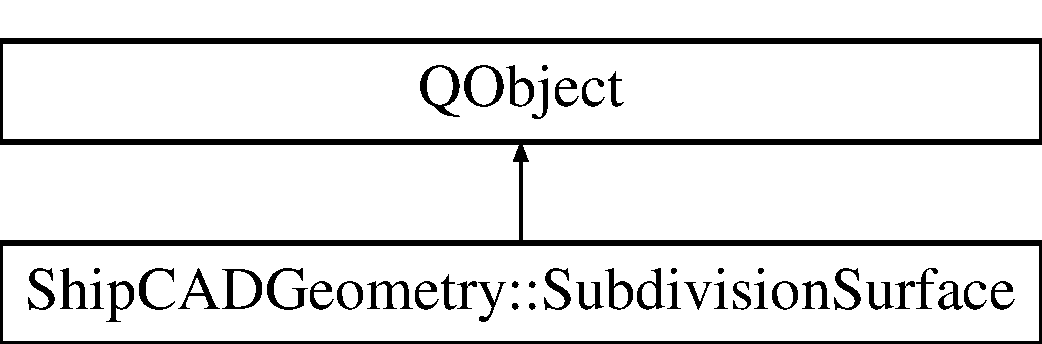
\includegraphics[height=2.000000cm]{classShipCADGeometry_1_1SubdivisionSurface}
\end{center}
\end{figure}
\subsection*{Public Types}
\begin{DoxyCompactItemize}
\item 
enum \hyperlink{classShipCADGeometry_1_1SubdivisionSurface_a0006dff46f8a47b8b37746602c6c2eca}{subdiv\-\_\-mode\-\_\-t} \{ \hyperlink{classShipCADGeometry_1_1SubdivisionSurface_a0006dff46f8a47b8b37746602c6c2ecaa3c3f0d6cce29361e4fd13198ff983bf4}{fm\-Quad\-Triangle}, 
\hyperlink{classShipCADGeometry_1_1SubdivisionSurface_a0006dff46f8a47b8b37746602c6c2ecaaf9dcd0c858b2f4efa96b21c8bc143ed4}{fm\-Catmull\-Clark}
 \}
\item 
enum \hyperlink{classShipCADGeometry_1_1SubdivisionSurface_a43e2c7b57684c6741bfd80506a19c33e}{assemble\-\_\-mode\-\_\-t} \{ \hyperlink{classShipCADGeometry_1_1SubdivisionSurface_a43e2c7b57684c6741bfd80506a19c33ea9f09992ff41262cb0a59e197364be338}{am\-Regular}, 
\hyperlink{classShipCADGeometry_1_1SubdivisionSurface_a43e2c7b57684c6741bfd80506a19c33ea155f4b7859879ebff4b7dcd2c9aedaf4}{am\-N\-U\-R\-B\-S}
 \}
\item 
typedef std\-::vector\\*
$<$ std\-::vector\\*
$<$ \hyperlink{classShipCADGeometry_1_1SubdivisionControlFace}{Subdivision\-Control\-Face} $\ast$ $>$ $>$ \hyperlink{classShipCADGeometry_1_1SubdivisionSurface_a9059895d23b9715aac304d3fecca12fb}{face\-\_\-grid\-\_\-t}
\item 
typedef std\-::vector\\*
$<$ std\-::vector\\*
$<$ \hyperlink{classShipCADGeometry_1_1SubdivisionPoint}{Subdivision\-Point} $\ast$ $>$ $>$ \hyperlink{classShipCADGeometry_1_1SubdivisionSurface_a360ddace48a5d6827e99a21e78a6c458}{grid\-\_\-t}
\item 
typedef std\-::vector\\*
$<$ std\-::vector\\*
$<$ \hyperlink{classShipCADGeometry_1_1SubdivisionControlPoint}{Subdivision\-Control\-Point} $\ast$ $>$ $>$ \hyperlink{classShipCADGeometry_1_1SubdivisionSurface_a515bffd2b65080a2c7f07ce98f82b026}{control\-\_\-grid\-\_\-t}
\item 
typedef std\-::vector\\*
$<$ std\-::vector$<$ Q\-Vector3\-D $>$ $>$ \hyperlink{classShipCADGeometry_1_1SubdivisionSurface_a89a36532eb6c7c2022258f8605fe929c}{coordinate\-\_\-grid\-\_\-t}
\end{DoxyCompactItemize}
\subsection*{Signals}
\begin{DoxyCompactItemize}
\item 
void \hyperlink{classShipCADGeometry_1_1SubdivisionSurface_a92e81f5ebe2eaf3098bab70eca4d6680}{changed\-Layer\-Data} ()
\item 
void \hyperlink{classShipCADGeometry_1_1SubdivisionSurface_acf56ae03aa0270d1f6703b781113f67a}{change\-Active\-Layer} ()
\item 
void \hyperlink{classShipCADGeometry_1_1SubdivisionSurface_a88100cb22d00cba4a0e3e0c347507f54}{select\-Item} (\hyperlink{classShipCADGeometry_1_1SubdivisionBase}{Subdivision\-Base} $\ast$)
\end{DoxyCompactItemize}
\subsection*{Public Member Functions}
\begin{DoxyCompactItemize}
\item 
\hyperlink{classShipCADGeometry_1_1SubdivisionSurface_a507ea9cd5354e1d14fe24d52da505934}{Subdivision\-Surface} ()
\item 
virtual \hyperlink{classShipCADGeometry_1_1SubdivisionSurface_a4f1b66a4d9e9f8ac3dbd956e2113a594}{$\sim$\-Subdivision\-Surface} ()
\item 
virtual void \hyperlink{classShipCADGeometry_1_1SubdivisionSurface_a80ab3bd6372a8465d69f71034a353e06}{clear} ()
\item 
void \hyperlink{classShipCADGeometry_1_1SubdivisionSurface_a13cfd2714344c9b85aad8d123538db48}{initialize} (size\-\_\-t point\-\_\-start, size\-\_\-t edge\-\_\-start)
\item 
void \hyperlink{classShipCADGeometry_1_1SubdivisionSurface_a259856fc21f2bc1eebbc52f10dd59469}{rebuild} ()
\item 
void \hyperlink{classShipCADGeometry_1_1SubdivisionSurface_ad140279118fab3343a6aee5e544814ec}{assemble\-Faces\-To\-Patches} (std\-::vector$<$ \hyperlink{classShipCADGeometry_1_1SubdivisionLayer}{Subdivision\-Layer} $\ast$ $>$ \&layers, \hyperlink{classShipCADGeometry_1_1SubdivisionSurface_a43e2c7b57684c6741bfd80506a19c33e}{assemble\-\_\-mode\-\_\-t} mode, std\-::vector$<$ \hyperlink{classShipCADGeometry_1_1SubdivisionFace}{Subdivision\-Face} $\ast$ $>$ \&assembled\-Patches, size\-\_\-t \&n\-Assembled)
\item 
void \hyperlink{classShipCADGeometry_1_1SubdivisionSurface_a3aa7c4fd1fa84170a59e6c0549573c92}{calculate\-Gauss\-Curvature} ()
\item 
void \hyperlink{classShipCADGeometry_1_1SubdivisionSurface_a2a984cc9ae8c78153113552cfb6321d5}{clear\-Selection} ()
\item 
void \hyperlink{classShipCADGeometry_1_1SubdivisionSurface_a1deabf43f6a24c34a58889d0361b0959}{convert\-To\-Grid} (\hyperlink{classShipCADGeometry_1_1SubdivisionSurface_a9059895d23b9715aac304d3fecca12fb}{face\-\_\-grid\-\_\-t} \&input, \hyperlink{classShipCADGeometry_1_1SubdivisionSurface_a360ddace48a5d6827e99a21e78a6c458}{grid\-\_\-t} \&grid)
\item 
void \hyperlink{classShipCADGeometry_1_1SubdivisionSurface_aa0460120d8a093682ca352a47affdb87}{edge\-Connect} ()
\item 
void \hyperlink{classShipCADGeometry_1_1SubdivisionSurface_abc1cf0168290242dfbe5dd0d178fa7cb}{extents} (Q\-Vector3\-D \&min, Q\-Vector3\-D \&max)
\item 
void \hyperlink{classShipCADGeometry_1_1SubdivisionSurface_ac19570e1402deab738d2231d6bec9650}{extrude\-Edges} (std\-::vector$<$ \hyperlink{classShipCADGeometry_1_1SubdivisionControlEdge}{Subdivision\-Control\-Edge} $\ast$ $>$ \&edges, const Q\-Vector3\-D \&direction)
\item 
void \hyperlink{classShipCADGeometry_1_1SubdivisionSurface_a576a4d43e01ca50782ba724f63f1b2bd}{calculate\-Intersections} (const \hyperlink{classShipCADGeometry_1_1Plane}{Plane} \&plane, std\-::vector$<$ \hyperlink{classShipCADGeometry_1_1SubdivisionControlFace}{Subdivision\-Control\-Face} $\ast$ $>$ \&faces, std\-::vector$<$ \hyperlink{classShipCADGeometry_1_1Spline}{Spline} $\ast$ $>$ \&destination)
\item 
void \hyperlink{classShipCADGeometry_1_1SubdivisionSurface_a17dccf4965b49427d345bd5acce897c5}{extract\-All\-Edge\-Loops} (std\-::vector$<$ std\-::vector$<$ \hyperlink{classShipCADGeometry_1_1SubdivisionPoint}{Subdivision\-Point} $\ast$ $>$ $>$ \&destination)
\item 
void \hyperlink{classShipCADGeometry_1_1SubdivisionSurface_af62ba549d058dfddd4bfa1b69a577220}{extract\-Points\-From\-Faces} (std\-::vector$<$ \hyperlink{classShipCADGeometry_1_1SubdivisionFace}{Subdivision\-Face} $\ast$ $>$ \&selectedfaces, std\-::vector$<$ \hyperlink{classShipCADGeometry_1_1SubdivisionControlPoint}{Subdivision\-Control\-Point} $\ast$ $>$ \&points, size\-\_\-t \&lockedpoints)
\item 
void \hyperlink{classShipCADGeometry_1_1SubdivisionSurface_af0f0d7bb979c8c8ba04b9be26e7cfe30}{extract\-Points\-From\-Selection} (std\-::vector$<$ \hyperlink{classShipCADGeometry_1_1SubdivisionControlPoint}{Subdivision\-Control\-Point} $\ast$ $>$ \&selectedpoints, size\-\_\-t \&lockedpoints)
\item 
void \hyperlink{classShipCADGeometry_1_1SubdivisionSurface_aa193fd28425e9846908479615e7c5bf9}{import\-Grid} (\hyperlink{classShipCADGeometry_1_1SubdivisionSurface_a89a36532eb6c7c2022258f8605fe929c}{coordinate\-\_\-grid\-\_\-t} \&points, \hyperlink{classShipCADGeometry_1_1SubdivisionLayer}{Subdivision\-Layer} $\ast$layer)
\item 
bool \hyperlink{classShipCADGeometry_1_1SubdivisionSurface_ab7191008f7ec3ef34b578b27e4340927}{intersect\-Plane} (const \hyperlink{classShipCADGeometry_1_1Plane}{Plane} \&plane, bool hydrostatics\-\_\-layers\-\_\-only, std\-::vector$<$ \hyperlink{classShipCADGeometry_1_1Spline}{Spline} $\ast$ $>$ \&destination)
\item 
void \hyperlink{classShipCADGeometry_1_1SubdivisionSurface_ada26b740ea1f317763b6ecd372f13ea2}{insert\-Plane} (const \hyperlink{classShipCADGeometry_1_1Plane}{Plane} \&plane, bool add\-\_\-curves)
\item 
void \hyperlink{classShipCADGeometry_1_1SubdivisionSurface_ad9970c667fa8e33ff8b35eb6a48b6a2e}{subdivide} ()
\item 
void \hyperlink{classShipCADGeometry_1_1SubdivisionSurface_a99bda5b49300775eda1df60451412686}{selection\-Delete} ()
\item 
size\-\_\-t \hyperlink{classShipCADGeometry_1_1SubdivisionSurface_a771f0f1881a2da57dde8cb88a8fc9059}{number\-Of\-Locked\-Points} ()
\item 
size\-\_\-t \hyperlink{classShipCADGeometry_1_1SubdivisionSurface_a2583bc0013b5725ac0902062d1c8bcea}{number\-Of\-Selected\-Locked\-Points} ()
\item 
size\-\_\-t \hyperlink{classShipCADGeometry_1_1SubdivisionSurface_a3778b3458f63987b5ef6dd482e6edc13}{number\-Of\-Points} ()
\item 
size\-\_\-t \hyperlink{classShipCADGeometry_1_1SubdivisionSurface_a1bde01d6b5972c302ad387cf1247f0fa}{index\-Of\-Point} (\hyperlink{classShipCADGeometry_1_1SubdivisionPoint}{Subdivision\-Point} $\ast$pt)
\item 
\hyperlink{classShipCADGeometry_1_1SubdivisionPoint}{Subdivision\-Point} $\ast$ \hyperlink{classShipCADGeometry_1_1SubdivisionSurface_af07192c8cfc3429ad6da80a1da802a6c}{get\-Point} (size\-\_\-t index)
\item 
void \hyperlink{classShipCADGeometry_1_1SubdivisionSurface_a4117039bfd819cb28ab5cb04296fdcd7}{delete\-Point} (\hyperlink{classShipCADGeometry_1_1SubdivisionPoint}{Subdivision\-Point} $\ast$pt)
\item 
size\-\_\-t \hyperlink{classShipCADGeometry_1_1SubdivisionSurface_ae965f02af93afdd0b164d39af6c38ce3}{number\-Of\-Control\-Points} ()
\item 
size\-\_\-t \hyperlink{classShipCADGeometry_1_1SubdivisionSurface_ae0dda53669e5767da6434b3e2f751916}{index\-Of\-Control\-Point} (\hyperlink{classShipCADGeometry_1_1SubdivisionControlPoint}{Subdivision\-Control\-Point} $\ast$pt)
\item 
bool \hyperlink{classShipCADGeometry_1_1SubdivisionSurface_a62abb29703f608a75559452d25db9a33}{has\-Control\-Point} (\hyperlink{classShipCADGeometry_1_1SubdivisionControlPoint}{Subdivision\-Control\-Point} $\ast$pt)
\item 
void \hyperlink{classShipCADGeometry_1_1SubdivisionSurface_aa20b9227481180329e03de8897c52933}{remove\-Control\-Point} (\hyperlink{classShipCADGeometry_1_1SubdivisionControlPoint}{Subdivision\-Control\-Point} $\ast$pt)
\item 
\hyperlink{classShipCADGeometry_1_1SubdivisionControlPoint}{Subdivision\-Control\-Point} $\ast$ \hyperlink{classShipCADGeometry_1_1SubdivisionSurface_a8aa8d3fdfc5e81ba4a39858a69228652}{get\-Control\-Point} (size\-\_\-t index)
\item 
\hyperlink{classShipCADGeometry_1_1SubdivisionControlPoint}{Subdivision\-Control\-Point} $\ast$ \hyperlink{classShipCADGeometry_1_1SubdivisionSurface_af644edd0d4ba993dbab280f036b37171}{add\-Control\-Point} (const Q\-Vector3\-D \&pt)
\item 
void \hyperlink{classShipCADGeometry_1_1SubdivisionSurface_a7ac8b717bcb728da2334cc2f16c8b428}{add\-Control\-Point} (\hyperlink{classShipCADGeometry_1_1SubdivisionControlPoint}{Subdivision\-Control\-Point} $\ast$pt)
\item 
\hyperlink{classShipCADGeometry_1_1SubdivisionControlPoint}{Subdivision\-Control\-Point} $\ast$ \hyperlink{classShipCADGeometry_1_1SubdivisionSurface_a7eccf33cb39ef12f56553352da34da62}{add\-Control\-Point} ()
\item 
void \hyperlink{classShipCADGeometry_1_1SubdivisionSurface_ad4f874132a137e89a39e60572748dab0}{delete\-Control\-Point} (\hyperlink{classShipCADGeometry_1_1SubdivisionControlPoint}{Subdivision\-Control\-Point} $\ast$point)
\item 
size\-\_\-t \hyperlink{classShipCADGeometry_1_1SubdivisionSurface_aedbc306bdce5691ff96a3a1eeb9aaece}{number\-Of\-Selected\-Control\-Points} ()
\item 
bool \hyperlink{classShipCADGeometry_1_1SubdivisionSurface_aafd696ac2c5353ac5593acdbe8b1fb2e}{has\-Selected\-Control\-Point} (\hyperlink{classShipCADGeometry_1_1SubdivisionControlPoint}{Subdivision\-Control\-Point} $\ast$pt)
\item 
void \hyperlink{classShipCADGeometry_1_1SubdivisionSurface_a65cc43d93da8ed72af631e893057c773}{set\-Selected\-Control\-Point} (\hyperlink{classShipCADGeometry_1_1SubdivisionControlPoint}{Subdivision\-Control\-Point} $\ast$pt)
\item 
void \hyperlink{classShipCADGeometry_1_1SubdivisionSurface_a5be891c06dc5e441511fbdb73d71efeb}{remove\-Selected\-Control\-Point} (\hyperlink{classShipCADGeometry_1_1SubdivisionControlPoint}{Subdivision\-Control\-Point} $\ast$pt)
\item 
size\-\_\-t \hyperlink{classShipCADGeometry_1_1SubdivisionSurface_a9315e6e9d5825ff3e3ba469fe4631e57}{number\-Of\-Edges} ()
\item 
size\-\_\-t \hyperlink{classShipCADGeometry_1_1SubdivisionSurface_aa3d68eacb2fafd9dab6d40c3230ed991}{index\-Of\-Edge} (\hyperlink{classShipCADGeometry_1_1SubdivisionEdge}{Subdivision\-Edge} $\ast$edge)
\item 
\hyperlink{classShipCADGeometry_1_1SubdivisionEdge}{Subdivision\-Edge} $\ast$ \hyperlink{classShipCADGeometry_1_1SubdivisionSurface_a67e69fc54ca38627596efc49b6d82e7f}{get\-Edge} (size\-\_\-t index)
\item 
\hyperlink{classShipCADGeometry_1_1SubdivisionEdge}{Subdivision\-Edge} $\ast$ \hyperlink{classShipCADGeometry_1_1SubdivisionSurface_adfdeabdc19eb55a7ba4ab0b607207300}{edge\-Exists} (\hyperlink{classShipCADGeometry_1_1SubdivisionPoint}{Subdivision\-Point} $\ast$p1, \hyperlink{classShipCADGeometry_1_1SubdivisionPoint}{Subdivision\-Point} $\ast$p2)
\item 
void \hyperlink{classShipCADGeometry_1_1SubdivisionSurface_abb5beb9a6fc413e8d713e18fb39bf2ba}{delete\-Edge} (\hyperlink{classShipCADGeometry_1_1SubdivisionEdge}{Subdivision\-Edge} $\ast$edge)
\item 
size\-\_\-t \hyperlink{classShipCADGeometry_1_1SubdivisionSurface_aa3647f3aec2f2c40ba764540cb29e7a2}{number\-Of\-Control\-Edges} ()
\item 
size\-\_\-t \hyperlink{classShipCADGeometry_1_1SubdivisionSurface_ae2f4e931f0134f8637e0aa769dba1d32}{index\-Of\-Control\-Edge} (\hyperlink{classShipCADGeometry_1_1SubdivisionControlEdge}{Subdivision\-Control\-Edge} $\ast$edge)
\item 
\hyperlink{classShipCADGeometry_1_1SubdivisionControlEdge}{Subdivision\-Control\-Edge} $\ast$ \hyperlink{classShipCADGeometry_1_1SubdivisionSurface_ac7d6762dc83f1f114c1d7f4e67d8f8eb}{get\-Control\-Edge} (size\-\_\-t index)
\item 
bool \hyperlink{classShipCADGeometry_1_1SubdivisionSurface_a9856bef9e5b2de9be4a3118fa80d0f16}{has\-Control\-Edge} (\hyperlink{classShipCADGeometry_1_1SubdivisionControlEdge}{Subdivision\-Control\-Edge} $\ast$edge)
\item 
\hyperlink{classShipCADGeometry_1_1SubdivisionControlEdge}{Subdivision\-Control\-Edge} $\ast$ \hyperlink{classShipCADGeometry_1_1SubdivisionSurface_a976358235d20a0fdc83248948bb9cf48}{add\-Control\-Edge} (\hyperlink{classShipCADGeometry_1_1SubdivisionPoint}{Subdivision\-Point} $\ast$sp, \hyperlink{classShipCADGeometry_1_1SubdivisionPoint}{Subdivision\-Point} $\ast$ep)
\item 
void \hyperlink{classShipCADGeometry_1_1SubdivisionSurface_a1f5ab04c4543f5084c1190fd788d8f63}{add\-Control\-Edge} (\hyperlink{classShipCADGeometry_1_1SubdivisionControlEdge}{Subdivision\-Control\-Edge} $\ast$edge)
\item 
\hyperlink{classShipCADGeometry_1_1SubdivisionControlEdge}{Subdivision\-Control\-Edge} $\ast$ \hyperlink{classShipCADGeometry_1_1SubdivisionSurface_a6a89be4440e3adfcb0b14c164db891ae}{control\-Edge\-Exists} (\hyperlink{classShipCADGeometry_1_1SubdivisionPoint}{Subdivision\-Point} $\ast$p1, \hyperlink{classShipCADGeometry_1_1SubdivisionPoint}{Subdivision\-Point} $\ast$p2)
\item 
void \hyperlink{classShipCADGeometry_1_1SubdivisionSurface_a3aac4d6c8ad638234f88fb8b1ffa00cb}{remove\-Control\-Edge} (\hyperlink{classShipCADGeometry_1_1SubdivisionControlEdge}{Subdivision\-Control\-Edge} $\ast$edge)
\item 
void \hyperlink{classShipCADGeometry_1_1SubdivisionSurface_ae45fc2694977c8fbae54ac2e0e067d1f}{delete\-Control\-Edge} (\hyperlink{classShipCADGeometry_1_1SubdivisionControlEdge}{Subdivision\-Control\-Edge} $\ast$edge)
\item 
void \hyperlink{classShipCADGeometry_1_1SubdivisionSurface_a975c97ca338eb2aaaa3dcc0640611a95}{isolate\-Edges} (std\-::vector$<$ \hyperlink{classShipCADGeometry_1_1SubdivisionControlEdge}{Subdivision\-Control\-Edge} $\ast$ $>$ \&input, std\-::vector$<$ std\-::vector$<$ \hyperlink{classShipCADGeometry_1_1SubdivisionControlPoint}{Subdivision\-Control\-Point} $\ast$ $>$ $>$ \&sorted)
\item 
size\-\_\-t \hyperlink{classShipCADGeometry_1_1SubdivisionSurface_ad414c410701ec58b0e3d064394fc4ddf}{number\-Of\-Selected\-Control\-Edges} ()
\item 
void \hyperlink{classShipCADGeometry_1_1SubdivisionSurface_ae1ceb8323935d0734fe4dc9c324aca16}{set\-Selected\-Control\-Edge} (\hyperlink{classShipCADGeometry_1_1SubdivisionControlEdge}{Subdivision\-Control\-Edge} $\ast$edge)
\item 
void \hyperlink{classShipCADGeometry_1_1SubdivisionSurface_a579077d742f9afc4e1d4ad20ef5a2184}{remove\-Selected\-Control\-Edge} (\hyperlink{classShipCADGeometry_1_1SubdivisionControlEdge}{Subdivision\-Control\-Edge} $\ast$edge)
\item 
bool \hyperlink{classShipCADGeometry_1_1SubdivisionSurface_a3f7856ea95b0c881a1171845c1dc817e}{has\-Selected\-Control\-Edge} (\hyperlink{classShipCADGeometry_1_1SubdivisionControlEdge}{Subdivision\-Control\-Edge} $\ast$edge)
\item 
size\-\_\-t \hyperlink{classShipCADGeometry_1_1SubdivisionSurface_a9f67bb8bbd3a8f61a2b4abacc0cf10e4}{number\-Of\-Faces} ()
\item 
void \hyperlink{classShipCADGeometry_1_1SubdivisionSurface_abf11847b9df1bc590c6c51d292430dd5}{clear\-Faces} ()
\item 
size\-\_\-t \hyperlink{classShipCADGeometry_1_1SubdivisionSurface_aefa41641c3665a22adebc66328eb51f7}{number\-Of\-Control\-Faces} ()
\item 
size\-\_\-t \hyperlink{classShipCADGeometry_1_1SubdivisionSurface_aee61b8795a0f16c47df83f0ef0abd2e7}{index\-Of\-Control\-Face} (\hyperlink{classShipCADGeometry_1_1SubdivisionControlFace}{Subdivision\-Control\-Face} $\ast$face)
\item 
\hyperlink{classShipCADGeometry_1_1SubdivisionControlFace}{Subdivision\-Control\-Face} $\ast$ \hyperlink{classShipCADGeometry_1_1SubdivisionSurface_a392f052a12118427919b910e99663d92}{get\-Control\-Face} (size\-\_\-t index)
\item 
\hyperlink{classShipCADGeometry_1_1SubdivisionControlFace}{Subdivision\-Control\-Face} $\ast$ \hyperlink{classShipCADGeometry_1_1SubdivisionSurface_a536574cc453e4790a769a3e7d47b7ff1}{get\-Control\-Face} (\hyperlink{classShipCADGeometry_1_1SubdivisionPoint}{Subdivision\-Point} $\ast$p1, \hyperlink{classShipCADGeometry_1_1SubdivisionPoint}{Subdivision\-Point} $\ast$p2, \hyperlink{classShipCADGeometry_1_1SubdivisionPoint}{Subdivision\-Point} $\ast$p3, \hyperlink{classShipCADGeometry_1_1SubdivisionPoint}{Subdivision\-Point} $\ast$p4)
\item 
bool \hyperlink{classShipCADGeometry_1_1SubdivisionSurface_ad6e00013faf6c373bfc1421adb941ba4}{has\-Control\-Face} (\hyperlink{classShipCADGeometry_1_1SubdivisionControlFace}{Subdivision\-Control\-Face} $\ast$face)
\item 
void \hyperlink{classShipCADGeometry_1_1SubdivisionSurface_abbbb7422a86771451034d2fb7a76bb26}{add\-Control\-Face} (\hyperlink{classShipCADGeometry_1_1SubdivisionControlFace}{Subdivision\-Control\-Face} $\ast$face)
\item 
\hyperlink{classShipCADGeometry_1_1SubdivisionControlFace}{Subdivision\-Control\-Face} $\ast$ \hyperlink{classShipCADGeometry_1_1SubdivisionSurface_a7c83a514f43b868b5fa286f3bc05a41e}{add\-Control\-Face} (std\-::vector$<$ Q\-Vector3\-D $>$ \&points)
\item 
\hyperlink{classShipCADGeometry_1_1SubdivisionControlFace}{Subdivision\-Control\-Face} $\ast$ \hyperlink{classShipCADGeometry_1_1SubdivisionSurface_a957b534788873921249cd1cc058b9d7e}{add\-Control\-Face} (std\-::vector$<$ \hyperlink{classShipCADGeometry_1_1SubdivisionControlPoint}{Subdivision\-Control\-Point} $\ast$ $>$ \&points, bool check\-\_\-edges)
\item 
\hyperlink{classShipCADGeometry_1_1SubdivisionControlFace}{Subdivision\-Control\-Face} $\ast$ \hyperlink{classShipCADGeometry_1_1SubdivisionSurface_a07d8ca69ed3d45f6e54407fcca8264b2}{add\-Control\-Face} (std\-::vector$<$ \hyperlink{classShipCADGeometry_1_1SubdivisionControlPoint}{Subdivision\-Control\-Point} $\ast$ $>$ \&points, bool check\-\_\-edges, \hyperlink{classShipCADGeometry_1_1SubdivisionLayer}{Subdivision\-Layer} $\ast$layer)
\item 
void \hyperlink{classShipCADGeometry_1_1SubdivisionSurface_a9cce3014753c0b74517b1747a80f6c2c}{remove\-Control\-Face} (\hyperlink{classShipCADGeometry_1_1SubdivisionControlFace}{Subdivision\-Control\-Face} $\ast$face)
\item 
void \hyperlink{classShipCADGeometry_1_1SubdivisionSurface_a394c490440fb20c37abfc2f38d6e50fd}{delete\-Control\-Face} (\hyperlink{classShipCADGeometry_1_1SubdivisionControlFace}{Subdivision\-Control\-Face} $\ast$face)
\item 
size\-\_\-t \hyperlink{classShipCADGeometry_1_1SubdivisionSurface_a98712984f4b918712ece45f32c4269fb}{number\-Of\-Selected\-Control\-Faces} ()
\item 
void \hyperlink{classShipCADGeometry_1_1SubdivisionSurface_ab21694a435e0c0dd6139de28ae543254}{set\-Selected\-Control\-Face} (\hyperlink{classShipCADGeometry_1_1SubdivisionControlFace}{Subdivision\-Control\-Face} $\ast$face)
\item 
void \hyperlink{classShipCADGeometry_1_1SubdivisionSurface_aef09d950b0970bd825a984effeee6224}{remove\-Selected\-Control\-Face} (\hyperlink{classShipCADGeometry_1_1SubdivisionControlFace}{Subdivision\-Control\-Face} $\ast$face)
\item 
bool \hyperlink{classShipCADGeometry_1_1SubdivisionSurface_aab0e513988645c868676831ae0093a25}{has\-Selected\-Control\-Face} (\hyperlink{classShipCADGeometry_1_1SubdivisionControlFace}{Subdivision\-Control\-Face} $\ast$face)
\item 
size\-\_\-t \hyperlink{classShipCADGeometry_1_1SubdivisionSurface_afd7bc97f31daf354830f234c205f4599}{number\-Of\-Control\-Curves} ()
\item 
size\-\_\-t \hyperlink{classShipCADGeometry_1_1SubdivisionSurface_af086dba8dcfe925ff9c814e6c72c44e8}{index\-Of\-Control\-Curve} (\hyperlink{classShipCADGeometry_1_1SubdivisionControlCurve}{Subdivision\-Control\-Curve} $\ast$curve)
\item 
\hyperlink{classShipCADGeometry_1_1SubdivisionControlCurve}{Subdivision\-Control\-Curve} $\ast$ \hyperlink{classShipCADGeometry_1_1SubdivisionSurface_a732c53d18277a4093ff7df12c0b08634}{get\-Control\-Curve} (size\-\_\-t index)
\item 
bool \hyperlink{classShipCADGeometry_1_1SubdivisionSurface_acc30feeff1a889b9b291dcab3987b30a}{has\-Control\-Curve} (\hyperlink{classShipCADGeometry_1_1SubdivisionControlCurve}{Subdivision\-Control\-Curve} $\ast$curve)
\item 
void \hyperlink{classShipCADGeometry_1_1SubdivisionSurface_aa01ccc2ce7417960ca13075e38eb98e6}{add\-Control\-Curve} (\hyperlink{classShipCADGeometry_1_1SubdivisionControlCurve}{Subdivision\-Control\-Curve} $\ast$curve)
\item 
void \hyperlink{classShipCADGeometry_1_1SubdivisionSurface_abd51f7744580144550fabc086ea991b4}{remove\-Control\-Curve} (\hyperlink{classShipCADGeometry_1_1SubdivisionControlCurve}{Subdivision\-Control\-Curve} $\ast$curve)
\item 
size\-\_\-t \hyperlink{classShipCADGeometry_1_1SubdivisionSurface_afe8e08b4471e106cfae40b3aa7e00f8e}{number\-Of\-Selected\-Control\-Curves} ()
\item 
void \hyperlink{classShipCADGeometry_1_1SubdivisionSurface_a5614a6ea5e1b67ec516328d64574cd9e}{set\-Selected\-Control\-Curve} (\hyperlink{classShipCADGeometry_1_1SubdivisionControlCurve}{Subdivision\-Control\-Curve} $\ast$curve)
\item 
void \hyperlink{classShipCADGeometry_1_1SubdivisionSurface_a1666628c8232ba11d386641fa7980ed7}{remove\-Selected\-Control\-Curve} (\hyperlink{classShipCADGeometry_1_1SubdivisionControlCurve}{Subdivision\-Control\-Curve} $\ast$curve)
\item 
bool \hyperlink{classShipCADGeometry_1_1SubdivisionSurface_acdfbfb4870bf517cd075fdf51a0de997}{has\-Selected\-Control\-Curve} (\hyperlink{classShipCADGeometry_1_1SubdivisionControlCurve}{Subdivision\-Control\-Curve} $\ast$curve)
\item 
size\-\_\-t \hyperlink{classShipCADGeometry_1_1SubdivisionSurface_a5dc4e6210058c2648bc7adefdf90c949}{number\-Of\-Layers} ()
\item 
size\-\_\-t \hyperlink{classShipCADGeometry_1_1SubdivisionSurface_accb1e8604e44f491f84e9fb77d1ab5c7}{index\-Of\-Layer} (\hyperlink{classShipCADGeometry_1_1SubdivisionLayer}{Subdivision\-Layer} $\ast$layer)
\item 
\hyperlink{classShipCADGeometry_1_1SubdivisionLayer}{Subdivision\-Layer} $\ast$ \hyperlink{classShipCADGeometry_1_1SubdivisionSurface_a24b230e51a0c5fb3e7f51d0e2340eb9f}{get\-Layer} (size\-\_\-t index)
\item 
\hyperlink{classShipCADGeometry_1_1SubdivisionLayer}{Subdivision\-Layer} $\ast$ \hyperlink{classShipCADGeometry_1_1SubdivisionSurface_a3d5b8cb035b43b48e4a4a3cb11a5c230}{get\-Active\-Layer} ()
\item 
void \hyperlink{classShipCADGeometry_1_1SubdivisionSurface_a69bafa71111e562a52a089be99b47871}{set\-Active\-Layer} (\hyperlink{classShipCADGeometry_1_1SubdivisionLayer}{Subdivision\-Layer} $\ast$layer)
\item 
bool \hyperlink{classShipCADGeometry_1_1SubdivisionSurface_aef9fe9a74054b54292f7f64e0589743c}{has\-Layer} (\hyperlink{classShipCADGeometry_1_1SubdivisionLayer}{Subdivision\-Layer} $\ast$layer)
\item 
void \hyperlink{classShipCADGeometry_1_1SubdivisionSurface_a3f0dac49106056562a8b675c61918abe}{delete\-Layer} (\hyperlink{classShipCADGeometry_1_1SubdivisionLayer}{Subdivision\-Layer} $\ast$layer)
\item 
size\-\_\-t \hyperlink{classShipCADGeometry_1_1SubdivisionSurface_adc6b4fcef1874f8153d9297be3cee19e}{last\-Used\-Layer\-I\-D} ()
\item 
void \hyperlink{classShipCADGeometry_1_1SubdivisionSurface_a9a84fd8dab00f34bf6f4a1e6663e52a3}{set\-Last\-Used\-Layer\-I\-D} (size\-\_\-t newid)
\item 
size\-\_\-t \hyperlink{classShipCADGeometry_1_1SubdivisionSurface_a3af3a30b53d867b2b25f9ac9290a264a}{request\-New\-Layer\-I\-D} ()
\item 
\hyperlink{classShipCADGeometry_1_1SubdivisionLayer}{Subdivision\-Layer} $\ast$ \hyperlink{classShipCADGeometry_1_1SubdivisionSurface_a5bf8f452664e17dae636d4b66a66eba9}{add\-New\-Layer} ()
\item 
bool \hyperlink{classShipCADGeometry_1_1SubdivisionSurface_a4e7ac46da75513b4764ee35580a4e59f}{is\-Build} ()
\item 
void \hyperlink{classShipCADGeometry_1_1SubdivisionSurface_aec5073750762d1f8c3ab2107a742f4a5}{set\-Build} (bool val)
\item 
\hyperlink{classShipCADGeometry_1_1SubdivisionSurface_a0006dff46f8a47b8b37746602c6c2eca}{subdiv\-\_\-mode\-\_\-t} \hyperlink{classShipCADGeometry_1_1SubdivisionSurface_aa088371fc23ba3bd68f705c64a051734}{get\-Subdivision\-Mode} ()
\item 
void \hyperlink{classShipCADGeometry_1_1SubdivisionSurface_a048dce00d2ff87aa5b31319ea41f565a}{set\-Subdivision\-Mode} (\hyperlink{classShipCADGeometry_1_1SubdivisionSurface_a0006dff46f8a47b8b37746602c6c2eca}{subdiv\-\_\-mode\-\_\-t} val)
\item 
void \hyperlink{classShipCADGeometry_1_1SubdivisionSurface_a53271216c1be89154c08d2b2841f9a60}{set\-Desired\-Subdivision\-Level} (int val)
\item 
bool \hyperlink{classShipCADGeometry_1_1SubdivisionSurface_aa6e07e073f76fb31d013103c8709f923}{is\-Gauss\-Curvature\-Calculated} ()
\item 
float \hyperlink{classShipCADGeometry_1_1SubdivisionSurface_ae6e80283a5c978dac2c912b365e28127}{get\-Curvature\-Scale} ()
\item 
void \hyperlink{classShipCADGeometry_1_1SubdivisionSurface_a660c1de6bb820c26895d4abe05befa79}{set\-Curvature\-Scale} (float val)
\item 
float \hyperlink{classShipCADGeometry_1_1SubdivisionSurface_acd42c6cedf4c0986e93c9ab991b034be}{get\-Min\-Gaus\-Curvature} ()
\item 
float \hyperlink{classShipCADGeometry_1_1SubdivisionSurface_ad36b9da92eb1c41ec5cecc1635a91dd6}{get\-Max\-Gaus\-Curvature} ()
\item 
const \hyperlink{classShipCADGeometry_1_1Plane}{Plane} \& \hyperlink{classShipCADGeometry_1_1SubdivisionSurface_a2707c2ff8d33de67c1e7027fcb1dcbf2}{get\-Waterline\-Plane} ()
\item 
void \hyperlink{classShipCADGeometry_1_1SubdivisionSurface_a5e16740196e65aa6590d5816b5425fed}{set\-Waterline\-Plane} (const \hyperlink{classShipCADGeometry_1_1Plane}{Plane} \&val)
\item 
float \hyperlink{classShipCADGeometry_1_1SubdivisionSurface_abe54fc725cc253d946470fe6eb8b59a9}{get\-Mainframe\-Location} ()
\item 
void \hyperlink{classShipCADGeometry_1_1SubdivisionSurface_a8bfafae576716a8c98dad4db4c79b0f8}{set\-Mainframe\-Location} (float val)
\item 
int \hyperlink{classShipCADGeometry_1_1SubdivisionSurface_ad246b6511bb0d1877edeec53f6a48501}{get\-Control\-Point\-Size} ()
\item 
bool \hyperlink{classShipCADGeometry_1_1SubdivisionSurface_a5cfac5d230987823a2c67b9f1ef5b850}{show\-Curvature} ()
\item 
bool \hyperlink{classShipCADGeometry_1_1SubdivisionSurface_aa40e92058695659d80a4283a9d71f2e4}{shade\-Under\-Water} ()
\item 
bool \hyperlink{classShipCADGeometry_1_1SubdivisionSurface_a8bcb27aafb421ec73ee60f1a80fddb9d}{show\-Control\-Net} ()
\item 
bool \hyperlink{classShipCADGeometry_1_1SubdivisionSurface_a0d71d0c19d12fdfeeaa962d4f94f33fe}{show\-Control\-Curves} ()
\item 
bool \hyperlink{classShipCADGeometry_1_1SubdivisionSurface_af17854000a39122b592ee59d84132483}{show\-Interior\-Edges} ()
\item 
bool \hyperlink{classShipCADGeometry_1_1SubdivisionSurface_ab68edba6d7b7350a39d777200e71b5e1}{draw\-Mirror} ()
\item 
bool \hyperlink{classShipCADGeometry_1_1SubdivisionSurface_a69852b83026fd12dd2dea75d2c68839a}{show\-Normals} ()
\item 
void \hyperlink{classShipCADGeometry_1_1SubdivisionSurface_af59c8172e7578be54d689779c7da7099}{set\-Show\-Curvature} (bool val)
\item 
void \hyperlink{classShipCADGeometry_1_1SubdivisionSurface_a69f08c4bd0e51a8a5d73eab2218d5556}{set\-Shade\-Under\-Water} (bool val)
\item 
void \hyperlink{classShipCADGeometry_1_1SubdivisionSurface_a83fc1704bb991aa6a948f93bf7e36a93}{set\-Show\-Control\-Net} (bool val)
\item 
void \hyperlink{classShipCADGeometry_1_1SubdivisionSurface_a718b01ea4fcf3dcde81c7215fa5da9c8}{set\-Show\-Control\-Curves} (bool val)
\item 
void \hyperlink{classShipCADGeometry_1_1SubdivisionSurface_adfa9f3ad89905c093c878de1891bcf31}{set\-Show\-Interior\-Edges} (bool val)
\item 
void \hyperlink{classShipCADGeometry_1_1SubdivisionSurface_a5d5672a862147a445a45bcccff793994}{set\-Draw\-Mirror} (bool val)
\item 
void \hyperlink{classShipCADGeometry_1_1SubdivisionSurface_a0829b1761cfce60f5cd68f00a45a37a6}{set\-Show\-Normals} (bool val)
\item 
Q\-Color \hyperlink{classShipCADGeometry_1_1SubdivisionSurface_ad6695d1d6b1d1410f36be190d0361235}{get\-Selected\-Color} ()
\item 
Q\-Color \hyperlink{classShipCADGeometry_1_1SubdivisionSurface_a654de66b37e4094d6fb9b8a2e40a5de6}{get\-Crease\-Edge\-Color} ()
\item 
Q\-Color \hyperlink{classShipCADGeometry_1_1SubdivisionSurface_ab932f5a4313393e65a1627c2ba924840}{get\-Edge\-Color} ()
\item 
Q\-Color \hyperlink{classShipCADGeometry_1_1SubdivisionSurface_adc1408be06e16bcb0d02901ff4d6469f}{get\-Leak\-Color} ()
\item 
Q\-Color \hyperlink{classShipCADGeometry_1_1SubdivisionSurface_ae04ad2348396b33fe00b1e2b0ae58ea9}{get\-Regular\-Point\-Color} ()
\item 
Q\-Color \hyperlink{classShipCADGeometry_1_1SubdivisionSurface_a089168e9a8940de6ba2292793cce9d7a}{get\-Corner\-Point\-Color} ()
\item 
Q\-Color \hyperlink{classShipCADGeometry_1_1SubdivisionSurface_ad8726fdbb7089c8a2fa8306abccfec18}{get\-Dart\-Point\-Color} ()
\item 
Q\-Color \hyperlink{classShipCADGeometry_1_1SubdivisionSurface_a71f7f105790c4cdaf44a132c602fde34}{get\-Crease\-Color} ()
\item 
Q\-Color \hyperlink{classShipCADGeometry_1_1SubdivisionSurface_a86bb08b5eff00deb3fa597b3272d99f1}{get\-Crease\-Point\-Color} ()
\item 
Q\-Color \hyperlink{classShipCADGeometry_1_1SubdivisionSurface_a12e3f89533293e2ca2dfa1ec4fa4cb71}{get\-Control\-Curve\-Color} ()
\item 
Q\-Color \hyperlink{classShipCADGeometry_1_1SubdivisionSurface_ade918dfa52fb1254e4c3808639ee11c3}{get\-Layer\-Color} ()
\item 
Q\-Color \hyperlink{classShipCADGeometry_1_1SubdivisionSurface_a4b84d7479369659b284af39f8bb36909}{get\-Curvature\-Color} ()
\item 
void \hyperlink{classShipCADGeometry_1_1SubdivisionSurface_a6e6254ecc6fcbdadf1ff4f646caa1d59}{save\-Binary} (\hyperlink{classShipCADGeometry_1_1FileBuffer}{File\-Buffer} \&destination)
\item 
void \hyperlink{classShipCADGeometry_1_1SubdivisionSurface_ac8ad644e0c19ac180fd4a7368fa410a6}{load\-Binary} (\hyperlink{classShipCADGeometry_1_1FileBuffer}{File\-Buffer} \&source)
\item 
void \hyperlink{classShipCADGeometry_1_1SubdivisionSurface_a489eed6508bb376170fa7926d2b7dc10}{load\-From\-Stream} (size\-\_\-t \&lineno, std\-::vector$<$ Q\-String $>$ \&strings)
\item 
void \hyperlink{classShipCADGeometry_1_1SubdivisionSurface_a183437fe2ac34285846224c7c1bba01b}{load\-V\-R\-M\-L\-File} (const Q\-String \&filename)
\item 
void \hyperlink{classShipCADGeometry_1_1SubdivisionSurface_a958a2af5d8d06ccf1aa3ac4e812cb1be}{export\-Fe\-F\-File} (std\-::vector$<$ Q\-String $>$ \&strings)
\item 
void \hyperlink{classShipCADGeometry_1_1SubdivisionSurface_af5e99c578032b83916f5c06591cbf459}{import\-Fe\-F\-File} (std\-::vector$<$ Q\-String $>$ \&strings, size\-\_\-t \&lineno)
\item 
void \hyperlink{classShipCADGeometry_1_1SubdivisionSurface_ac6a4c0542b17b1b50edb57ea5c0f28ec}{export\-Obj\-File} (bool export\-\_\-control\-\_\-net, std\-::vector$<$ Q\-String $>$ \&strings)
\item 
void \hyperlink{classShipCADGeometry_1_1SubdivisionSurface_a51d2d07423cc53fc98012f07ed9525bc}{save\-To\-Stream} (std\-::vector$<$ Q\-String $>$ \&strings)
\item 
virtual void \hyperlink{classShipCADGeometry_1_1SubdivisionSurface_acfe9cc964dbe05105486b43f2dc6fc4f}{draw} (\hyperlink{classShipCADGeometry_1_1Viewport}{Viewport} \&vp)
\item 
virtual void \hyperlink{classShipCADGeometry_1_1SubdivisionSurface_a6ed961bbb7ca5fe94ec5566109d9b015}{dump} (std\-::ostream \&os, const char $\ast$prefix=\char`\"{}\char`\"{}) const 
\item 
boost\-::pool \& \hyperlink{classShipCADGeometry_1_1SubdivisionSurface_a9d5cdfe8f0fbbb50ab9614d54066d6cc}{get\-Control\-Point\-Pool} ()
\item 
boost\-::pool \& \hyperlink{classShipCADGeometry_1_1SubdivisionSurface_a87533a29f28e1ea0279c6ff48bdcfd85}{get\-Control\-Edge\-Pool} ()
\item 
boost\-::pool \& \hyperlink{classShipCADGeometry_1_1SubdivisionSurface_aa6e26bcb1436e1d1f83141309e3b8dd9}{get\-Control\-Face\-Pool} ()
\item 
boost\-::pool \& \hyperlink{classShipCADGeometry_1_1SubdivisionSurface_af31a65c4b4eb7022212979d7935ceaa6}{get\-Control\-Curve\-Pool} ()
\item 
boost\-::pool \& \hyperlink{classShipCADGeometry_1_1SubdivisionSurface_aa827f5ba825453c633e0f9e4e0153952}{get\-Layer\-Pool} ()
\item 
boost\-::pool \& \hyperlink{classShipCADGeometry_1_1SubdivisionSurface_ad2cdb88cf70335a06ee4a571ce256ee3}{get\-Point\-Pool} ()
\item 
boost\-::pool \& \hyperlink{classShipCADGeometry_1_1SubdivisionSurface_a4f84479805e2570cbfc1906ee812501c}{get\-Edge\-Pool} ()
\item 
boost\-::pool \& \hyperlink{classShipCADGeometry_1_1SubdivisionSurface_a40797b8fb8d4cc57064d2fc3356f4314}{get\-Face\-Pool} ()
\end{DoxyCompactItemize}
\subsection*{Protected Member Functions}
\begin{DoxyCompactItemize}
\item 
void \hyperlink{classShipCADGeometry_1_1SubdivisionSurface_a5c88eb988cc6a439242264bc54a6e3e1}{priv\-\_\-dump} (std\-::ostream \&os, const char $\ast$prefix) const 
\item 
\hyperlink{classShipCADGeometry_1_1SubdivisionControlPoint}{Subdivision\-Control\-Point} $\ast$ \hyperlink{classShipCADGeometry_1_1SubdivisionSurface_a251b711125d50aa51875451976e8a8d7}{new\-Control\-Point} (const Q\-Vector3\-D \&p)
\item 
void \hyperlink{classShipCADGeometry_1_1SubdivisionSurface_a3163cfd01e0454ecb9dbb088dc76fbc6}{find\-Attached\-Faces} (std\-::vector$<$ \hyperlink{classShipCADGeometry_1_1SubdivisionControlFace}{Subdivision\-Control\-Face} $\ast$ $>$ \&found\-\_\-list, std\-::vector$<$ \hyperlink{classShipCADGeometry_1_1SubdivisionControlFace}{Subdivision\-Control\-Face} $\ast$ $>$ \&todo\-\_\-list, \hyperlink{classShipCADGeometry_1_1SubdivisionControlFace}{Subdivision\-Control\-Face} $\ast$face)
\item 
bool \hyperlink{classShipCADGeometry_1_1SubdivisionSurface_a5b6204bb0648f2e85cbf07ffbac4bd42}{valid\-Face} (\hyperlink{classShipCADGeometry_1_1SubdivisionFace}{Subdivision\-Face} $\ast$face, std\-::vector$<$ \hyperlink{classShipCADGeometry_1_1SubdivisionFace}{Subdivision\-Face} $\ast$ $>$ \&faces, std\-::vector$<$ \hyperlink{classShipCADGeometry_1_1SubdivisionFace}{Subdivision\-Face} $\ast$ $>$ \&tmpfaces)
\item 
void \hyperlink{classShipCADGeometry_1_1SubdivisionSurface_ac322d8008ea13bc3ca3fd1baeab7e1b3}{do\-Assemble} (\hyperlink{classShipCADGeometry_1_1SubdivisionSurface_a360ddace48a5d6827e99a21e78a6c458}{grid\-\_\-t} \&grid, size\-\_\-t \&cols, size\-\_\-t \&rows, std\-::vector$<$ \hyperlink{classShipCADGeometry_1_1SubdivisionFace}{Subdivision\-Face} $\ast$ $>$ \&faces)
\item 
void \hyperlink{classShipCADGeometry_1_1SubdivisionSurface_a2b270b878bb810d51bd7adf689db5366}{sort\-Edges} (std\-::vector$<$ \hyperlink{classShipCADGeometry_1_1SubdivisionEdge}{Subdivision\-Edge} $\ast$ $>$ \&edges)
\item 
std\-::vector$<$ \hyperlink{classShipCADGeometry_1_1SubdivisionPoint}{Subdivision\-Point} $\ast$ $>$ \hyperlink{classShipCADGeometry_1_1SubdivisionSurface_abbabb02057a2e66d2a37ec84696788e9}{sort\-Edges} (bool always\-\_\-true, std\-::vector$<$ \hyperlink{classShipCADGeometry_1_1SubdivisionEdge}{Subdivision\-Edge} $\ast$ $>$ \&edges)
\item 
std\-::vector\\*
$<$ \hyperlink{classShipCADGeometry_1_1SubdivisionControlPoint}{Subdivision\-Control\-Point} $\ast$ $>$ \hyperlink{classShipCADGeometry_1_1SubdivisionSurface_a8650bf95c9eb2de0e0b1342bfacbe82a}{sort\-Edges} (std\-::vector$<$ \hyperlink{classShipCADGeometry_1_1SubdivisionControlEdge}{Subdivision\-Control\-Edge} $\ast$ $>$ \&edges)
\end{DoxyCompactItemize}
\subsection*{Protected Attributes}
\begin{DoxyCompactItemize}
\item 
bool \hyperlink{classShipCADGeometry_1_1SubdivisionSurface_abdb049451d948cc92be79719e03adfff}{\-\_\-build}
\item 
bool \hyperlink{classShipCADGeometry_1_1SubdivisionSurface_a6d4fdb7be66c662f86b397792c9dada8}{\-\_\-show\-\_\-control\-\_\-net}
\item 
bool \hyperlink{classShipCADGeometry_1_1SubdivisionSurface_a3276e7cb242a6f2bbc1730ca4b545264}{\-\_\-initialized}
\item 
bool \hyperlink{classShipCADGeometry_1_1SubdivisionSurface_a419375e351105466cb3d9ac2b739c94f}{\-\_\-show\-\_\-interior\-\_\-edges}
\item 
bool \hyperlink{classShipCADGeometry_1_1SubdivisionSurface_a6401966145eb3c364946cd045be6deb0}{\-\_\-draw\-\_\-mirror}
\item 
bool \hyperlink{classShipCADGeometry_1_1SubdivisionSurface_a53759454945841ea3f10c033e3524382}{\-\_\-shade\-\_\-under\-\_\-water}
\item 
bool \hyperlink{classShipCADGeometry_1_1SubdivisionSurface_a4e91054edb430c269d3c3d53e85e3f05}{\-\_\-show\-\_\-normals}
\item 
bool \hyperlink{classShipCADGeometry_1_1SubdivisionSurface_ab539a00832aa77ab899ba9db730d8aff}{\-\_\-show\-\_\-curvature}
\item 
bool \hyperlink{classShipCADGeometry_1_1SubdivisionSurface_a0d76f9d22bf18c13a74aa336922094bb}{\-\_\-show\-\_\-control\-\_\-curves}
\item 
\hyperlink{classShipCADGeometry_1_1SubdivisionSurface_a0006dff46f8a47b8b37746602c6c2eca}{subdiv\-\_\-mode\-\_\-t} \hyperlink{classShipCADGeometry_1_1SubdivisionSurface_ac44334fa73b1d714146df68752e143be}{\-\_\-subdivision\-\_\-mode}
\item 
int \hyperlink{classShipCADGeometry_1_1SubdivisionSurface_a4199f489017ebae8a9a2dc08248414e3}{\-\_\-desired\-\_\-subdiv\-\_\-level}
\item 
int \hyperlink{classShipCADGeometry_1_1SubdivisionSurface_ab1e864d6bd7858f3ad98177c6c288416}{\-\_\-current\-\_\-subdiv\-\_\-level}
\item 
int \hyperlink{classShipCADGeometry_1_1SubdivisionSurface_ae25d19f752c08bb54c821433032ae156}{\-\_\-control\-\_\-point\-\_\-size}
\item 
float \hyperlink{classShipCADGeometry_1_1SubdivisionSurface_af3a93d368f74ba66a38c5b8129625507}{\-\_\-curvature\-\_\-scale}
\item 
float \hyperlink{classShipCADGeometry_1_1SubdivisionSurface_a223facd5bb1129e64d71c30ceb715ca9}{\-\_\-min\-\_\-gaus\-\_\-curvature}
\item 
float \hyperlink{classShipCADGeometry_1_1SubdivisionSurface_afcea46c7f82ef5a320e8a70bdcb40eef}{\-\_\-max\-\_\-gaus\-\_\-curvature}
\item 
float \hyperlink{classShipCADGeometry_1_1SubdivisionSurface_a6fc67d1abe025264cceec88f7bcc10e7}{\-\_\-main\-\_\-frame\-\_\-location}
\item 
Q\-Color \hyperlink{classShipCADGeometry_1_1SubdivisionSurface_a5d7be8d94a41e44acf6ef075b5ff2c2f}{\-\_\-crease\-\_\-color}
\item 
Q\-Color \hyperlink{classShipCADGeometry_1_1SubdivisionSurface_a92ce4d932dd32da046a0fdae785d14a2}{\-\_\-crease\-\_\-edge\-\_\-color}
\item 
Q\-Color \hyperlink{classShipCADGeometry_1_1SubdivisionSurface_a5733dc4d79a050465e6d41c6c35a46a3}{\-\_\-underwater\-\_\-color}
\item 
Q\-Color \hyperlink{classShipCADGeometry_1_1SubdivisionSurface_a97992c6c6ab3953f4e3152433f786886}{\-\_\-edge\-\_\-color}
\item 
Q\-Color \hyperlink{classShipCADGeometry_1_1SubdivisionSurface_a07875af551f7dd1f31dc5c4beeb130fb}{\-\_\-selected\-\_\-color}
\item 
Q\-Color \hyperlink{classShipCADGeometry_1_1SubdivisionSurface_a64d0838f3bc37c1b67de7c8a98f77c6f}{\-\_\-crease\-\_\-point\-\_\-color}
\item 
Q\-Color \hyperlink{classShipCADGeometry_1_1SubdivisionSurface_a0f77d9f2a48f9fe4569508d2dac00325}{\-\_\-regular\-\_\-point\-\_\-color}
\item 
Q\-Color \hyperlink{classShipCADGeometry_1_1SubdivisionSurface_a1a258a7eb65fd759138f386ca88b158d}{\-\_\-corner\-\_\-point\-\_\-color}
\item 
Q\-Color \hyperlink{classShipCADGeometry_1_1SubdivisionSurface_ac55852997435d20440ef5f8a0605ee28}{\-\_\-dart\-\_\-point\-\_\-color}
\item 
Q\-Color \hyperlink{classShipCADGeometry_1_1SubdivisionSurface_ad0b4085cb1cb85de95664b13fe5ce088}{\-\_\-layer\-\_\-color}
\item 
Q\-Color \hyperlink{classShipCADGeometry_1_1SubdivisionSurface_a9c9c02173c424fe965e8906b5437a191}{\-\_\-normal\-\_\-color}
\item 
Q\-Color \hyperlink{classShipCADGeometry_1_1SubdivisionSurface_a802e546e42b45b2c379490ab72391914}{\-\_\-leak\-\_\-color}
\item 
Q\-Color \hyperlink{classShipCADGeometry_1_1SubdivisionSurface_a363d17c15f29781ef200e105e72886b1}{\-\_\-curvature\-\_\-color}
\item 
Q\-Color \hyperlink{classShipCADGeometry_1_1SubdivisionSurface_a83328b441440e91ccd1793024020769c}{\-\_\-control\-\_\-curve\-\_\-color}
\item 
Q\-Color \hyperlink{classShipCADGeometry_1_1SubdivisionSurface_a26726d15987c2985f5ba16fba5c470b7}{\-\_\-zebra\-\_\-color}
\item 
\hyperlink{classShipCADGeometry_1_1Plane}{Plane} \hyperlink{classShipCADGeometry_1_1SubdivisionSurface_aaa7e9b322884649fb506848a9b4e2994}{\-\_\-waterline\-\_\-plane}
\item 
Q\-Vector3\-D \hyperlink{classShipCADGeometry_1_1SubdivisionSurface_a7318c1fbfeb1f0fbb8b2f445d607e4ef}{\-\_\-min}
\item 
Q\-Vector3\-D \hyperlink{classShipCADGeometry_1_1SubdivisionSurface_ae206a579d516760512056460b9e0237c}{\-\_\-max}
\item 
size\-\_\-t \hyperlink{classShipCADGeometry_1_1SubdivisionSurface_a9e350ce7cffd0975d03fd3bea0c95967}{\-\_\-last\-\_\-used\-\_\-layer\-I\-D}
\item 
\hyperlink{classShipCADGeometry_1_1SubdivisionLayer}{Subdivision\-Layer} $\ast$ \hyperlink{classShipCADGeometry_1_1SubdivisionSurface_a11225d0db63ff0d314dba77e0340721f}{\-\_\-active\-\_\-layer}
\item 
std\-::vector\\*
$<$ \hyperlink{classShipCADGeometry_1_1SubdivisionControlPoint}{Subdivision\-Control\-Point} $\ast$ $>$ \hyperlink{classShipCADGeometry_1_1SubdivisionSurface_a7a1119ec998a0012e11ec7dee63073fc}{\-\_\-control\-\_\-points}
\item 
std\-::vector\\*
$<$ \hyperlink{classShipCADGeometry_1_1SubdivisionControlEdge}{Subdivision\-Control\-Edge} $\ast$ $>$ \hyperlink{classShipCADGeometry_1_1SubdivisionSurface_a430ba9ceba2a6423a007ea64b4566664}{\-\_\-control\-\_\-edges}
\item 
std\-::vector\\*
$<$ \hyperlink{classShipCADGeometry_1_1SubdivisionControlFace}{Subdivision\-Control\-Face} $\ast$ $>$ \hyperlink{classShipCADGeometry_1_1SubdivisionSurface_a34b2a606532616afdba7a5f71fd9efee}{\-\_\-control\-\_\-faces}
\item 
std\-::vector\\*
$<$ \hyperlink{classShipCADGeometry_1_1SubdivisionControlCurve}{Subdivision\-Control\-Curve} $\ast$ $>$ \hyperlink{classShipCADGeometry_1_1SubdivisionSurface_ae55f8fae758bd76dd3aaed737c61434c}{\-\_\-control\-\_\-curves}
\item 
std\-::vector$<$ \hyperlink{classShipCADGeometry_1_1SubdivisionLayer}{Subdivision\-Layer} $\ast$ $>$ \hyperlink{classShipCADGeometry_1_1SubdivisionSurface_adabe1dd268e280a6d21e3c546639175a}{\-\_\-layers}
\item 
std\-::vector$<$ float $>$ \hyperlink{classShipCADGeometry_1_1SubdivisionSurface_aa7f39e4d68d2b36a0a8ce3d6e386bce7}{\-\_\-gaus\-\_\-curvature}
\item 
std\-::vector$<$ \hyperlink{classShipCADGeometry_1_1SubdivisionPoint}{Subdivision\-Point} $\ast$ $>$ \hyperlink{classShipCADGeometry_1_1SubdivisionSurface_aee8defd15695208cd384c7e384b3525e}{\-\_\-points}
\item 
std\-::vector$<$ \hyperlink{classShipCADGeometry_1_1SubdivisionEdge}{Subdivision\-Edge} $\ast$ $>$ \hyperlink{classShipCADGeometry_1_1SubdivisionSurface_aeb49c9cecfb5bbf15e0983133e490cdf}{\-\_\-edges}
\item 
std\-::vector\\*
$<$ \hyperlink{classShipCADGeometry_1_1SubdivisionControlPoint}{Subdivision\-Control\-Point} $\ast$ $>$ \hyperlink{classShipCADGeometry_1_1SubdivisionSurface_a0a79167ca5f6a2604752a803dcc065da}{\-\_\-sel\-\_\-control\-\_\-points}
\item 
std\-::vector\\*
$<$ \hyperlink{classShipCADGeometry_1_1SubdivisionControlEdge}{Subdivision\-Control\-Edge} $\ast$ $>$ \hyperlink{classShipCADGeometry_1_1SubdivisionSurface_a0a93da68dbd5f8f29a2834a9410353d1}{\-\_\-sel\-\_\-control\-\_\-edges}
\item 
std\-::vector\\*
$<$ \hyperlink{classShipCADGeometry_1_1SubdivisionControlFace}{Subdivision\-Control\-Face} $\ast$ $>$ \hyperlink{classShipCADGeometry_1_1SubdivisionSurface_ad923194e92a6a88cbc9608c13a70436f}{\-\_\-sel\-\_\-control\-\_\-faces}
\item 
std\-::vector\\*
$<$ \hyperlink{classShipCADGeometry_1_1SubdivisionControlCurve}{Subdivision\-Control\-Curve} $\ast$ $>$ \hyperlink{classShipCADGeometry_1_1SubdivisionSurface_ad707edb71feec99421107e9664e393be}{\-\_\-sel\-\_\-control\-\_\-curves}
\item 
boost\-::pool \hyperlink{classShipCADGeometry_1_1SubdivisionSurface_aa9d50a7eea24cebe4e97f5af8dc0c4d8}{\-\_\-cpoint\-\_\-pool}
\item 
boost\-::pool \hyperlink{classShipCADGeometry_1_1SubdivisionSurface_ab66fbf875487bf60e8bfee2467ec62b0}{\-\_\-cedge\-\_\-pool}
\item 
boost\-::pool \hyperlink{classShipCADGeometry_1_1SubdivisionSurface_a4adedb7d11b2317d0ce08c650dd2f2cf}{\-\_\-cface\-\_\-pool}
\item 
boost\-::pool \hyperlink{classShipCADGeometry_1_1SubdivisionSurface_a832b507f17ba2220df2edfbb342e9f40}{\-\_\-ccurve\-\_\-pool}
\item 
boost\-::pool \hyperlink{classShipCADGeometry_1_1SubdivisionSurface_a3882857500f96a20d54bb484860186eb}{\-\_\-layer\-\_\-pool}
\item 
boost\-::pool \hyperlink{classShipCADGeometry_1_1SubdivisionSurface_a51b9089fd519e72564103a7b69ae7712}{\-\_\-point\-\_\-pool}
\item 
boost\-::pool \hyperlink{classShipCADGeometry_1_1SubdivisionSurface_a64367dcb560b1160baedd242fad08d5c}{\-\_\-edge\-\_\-pool}
\item 
boost\-::pool \hyperlink{classShipCADGeometry_1_1SubdivisionSurface_a66ebffe9b49fbdc29df0f3747affb786}{\-\_\-face\-\_\-pool}
\end{DoxyCompactItemize}


\subsection{Detailed Description}


Definition at line 66 of file subdivsurface.\-h.



\subsection{Member Typedef Documentation}
\hypertarget{classShipCADGeometry_1_1SubdivisionSurface_a515bffd2b65080a2c7f07ce98f82b026}{\index{Ship\-C\-A\-D\-Geometry\-::\-Subdivision\-Surface@{Ship\-C\-A\-D\-Geometry\-::\-Subdivision\-Surface}!control\-\_\-grid\-\_\-t@{control\-\_\-grid\-\_\-t}}
\index{control\-\_\-grid\-\_\-t@{control\-\_\-grid\-\_\-t}!ShipCADGeometry::SubdivisionSurface@{Ship\-C\-A\-D\-Geometry\-::\-Subdivision\-Surface}}
\subsubsection[{control\-\_\-grid\-\_\-t}]{\setlength{\rightskip}{0pt plus 5cm}typedef std\-::vector$<$std\-::vector$<${\bf Subdivision\-Control\-Point}$\ast$$>$ $>$ {\bf Ship\-C\-A\-D\-Geometry\-::\-Subdivision\-Surface\-::control\-\_\-grid\-\_\-t}}}\label{classShipCADGeometry_1_1SubdivisionSurface_a515bffd2b65080a2c7f07ce98f82b026}


Definition at line 74 of file subdivsurface.\-h.

\hypertarget{classShipCADGeometry_1_1SubdivisionSurface_a89a36532eb6c7c2022258f8605fe929c}{\index{Ship\-C\-A\-D\-Geometry\-::\-Subdivision\-Surface@{Ship\-C\-A\-D\-Geometry\-::\-Subdivision\-Surface}!coordinate\-\_\-grid\-\_\-t@{coordinate\-\_\-grid\-\_\-t}}
\index{coordinate\-\_\-grid\-\_\-t@{coordinate\-\_\-grid\-\_\-t}!ShipCADGeometry::SubdivisionSurface@{Ship\-C\-A\-D\-Geometry\-::\-Subdivision\-Surface}}
\subsubsection[{coordinate\-\_\-grid\-\_\-t}]{\setlength{\rightskip}{0pt plus 5cm}typedef std\-::vector$<$std\-::vector$<$Q\-Vector3\-D$>$ $>$ {\bf Ship\-C\-A\-D\-Geometry\-::\-Subdivision\-Surface\-::coordinate\-\_\-grid\-\_\-t}}}\label{classShipCADGeometry_1_1SubdivisionSurface_a89a36532eb6c7c2022258f8605fe929c}


Definition at line 75 of file subdivsurface.\-h.

\hypertarget{classShipCADGeometry_1_1SubdivisionSurface_a9059895d23b9715aac304d3fecca12fb}{\index{Ship\-C\-A\-D\-Geometry\-::\-Subdivision\-Surface@{Ship\-C\-A\-D\-Geometry\-::\-Subdivision\-Surface}!face\-\_\-grid\-\_\-t@{face\-\_\-grid\-\_\-t}}
\index{face\-\_\-grid\-\_\-t@{face\-\_\-grid\-\_\-t}!ShipCADGeometry::SubdivisionSurface@{Ship\-C\-A\-D\-Geometry\-::\-Subdivision\-Surface}}
\subsubsection[{face\-\_\-grid\-\_\-t}]{\setlength{\rightskip}{0pt plus 5cm}typedef std\-::vector$<$std\-::vector$<${\bf Subdivision\-Control\-Face}$\ast$$>$ $>$ {\bf Ship\-C\-A\-D\-Geometry\-::\-Subdivision\-Surface\-::face\-\_\-grid\-\_\-t}}}\label{classShipCADGeometry_1_1SubdivisionSurface_a9059895d23b9715aac304d3fecca12fb}


Definition at line 72 of file subdivsurface.\-h.

\hypertarget{classShipCADGeometry_1_1SubdivisionSurface_a360ddace48a5d6827e99a21e78a6c458}{\index{Ship\-C\-A\-D\-Geometry\-::\-Subdivision\-Surface@{Ship\-C\-A\-D\-Geometry\-::\-Subdivision\-Surface}!grid\-\_\-t@{grid\-\_\-t}}
\index{grid\-\_\-t@{grid\-\_\-t}!ShipCADGeometry::SubdivisionSurface@{Ship\-C\-A\-D\-Geometry\-::\-Subdivision\-Surface}}
\subsubsection[{grid\-\_\-t}]{\setlength{\rightskip}{0pt plus 5cm}typedef std\-::vector$<$std\-::vector$<${\bf Subdivision\-Point}$\ast$$>$ $>$ {\bf Ship\-C\-A\-D\-Geometry\-::\-Subdivision\-Surface\-::grid\-\_\-t}}}\label{classShipCADGeometry_1_1SubdivisionSurface_a360ddace48a5d6827e99a21e78a6c458}


Definition at line 73 of file subdivsurface.\-h.



\subsection{Member Enumeration Documentation}
\hypertarget{classShipCADGeometry_1_1SubdivisionSurface_a43e2c7b57684c6741bfd80506a19c33e}{\index{Ship\-C\-A\-D\-Geometry\-::\-Subdivision\-Surface@{Ship\-C\-A\-D\-Geometry\-::\-Subdivision\-Surface}!assemble\-\_\-mode\-\_\-t@{assemble\-\_\-mode\-\_\-t}}
\index{assemble\-\_\-mode\-\_\-t@{assemble\-\_\-mode\-\_\-t}!ShipCADGeometry::SubdivisionSurface@{Ship\-C\-A\-D\-Geometry\-::\-Subdivision\-Surface}}
\subsubsection[{assemble\-\_\-mode\-\_\-t}]{\setlength{\rightskip}{0pt plus 5cm}enum {\bf Ship\-C\-A\-D\-Geometry\-::\-Subdivision\-Surface\-::assemble\-\_\-mode\-\_\-t}}}\label{classShipCADGeometry_1_1SubdivisionSurface_a43e2c7b57684c6741bfd80506a19c33e}
\begin{Desc}
\item[Enumerator]\par
\begin{description}
\index{am\-Regular@{am\-Regular}!Ship\-C\-A\-D\-Geometry\-::\-Subdivision\-Surface@{Ship\-C\-A\-D\-Geometry\-::\-Subdivision\-Surface}}\index{Ship\-C\-A\-D\-Geometry\-::\-Subdivision\-Surface@{Ship\-C\-A\-D\-Geometry\-::\-Subdivision\-Surface}!am\-Regular@{am\-Regular}}\item[{\em 
\hypertarget{classShipCADGeometry_1_1SubdivisionSurface_a43e2c7b57684c6741bfd80506a19c33ea9f09992ff41262cb0a59e197364be338}{am\-Regular}\label{classShipCADGeometry_1_1SubdivisionSurface_a43e2c7b57684c6741bfd80506a19c33ea9f09992ff41262cb0a59e197364be338}
}]\index{am\-N\-U\-R\-B\-S@{am\-N\-U\-R\-B\-S}!Ship\-C\-A\-D\-Geometry\-::\-Subdivision\-Surface@{Ship\-C\-A\-D\-Geometry\-::\-Subdivision\-Surface}}\index{Ship\-C\-A\-D\-Geometry\-::\-Subdivision\-Surface@{Ship\-C\-A\-D\-Geometry\-::\-Subdivision\-Surface}!am\-N\-U\-R\-B\-S@{am\-N\-U\-R\-B\-S}}\item[{\em 
\hypertarget{classShipCADGeometry_1_1SubdivisionSurface_a43e2c7b57684c6741bfd80506a19c33ea155f4b7859879ebff4b7dcd2c9aedaf4}{am\-N\-U\-R\-B\-S}\label{classShipCADGeometry_1_1SubdivisionSurface_a43e2c7b57684c6741bfd80506a19c33ea155f4b7859879ebff4b7dcd2c9aedaf4}
}]\end{description}
\end{Desc}


Definition at line 78 of file subdivsurface.\-h.

\hypertarget{classShipCADGeometry_1_1SubdivisionSurface_a0006dff46f8a47b8b37746602c6c2eca}{\index{Ship\-C\-A\-D\-Geometry\-::\-Subdivision\-Surface@{Ship\-C\-A\-D\-Geometry\-::\-Subdivision\-Surface}!subdiv\-\_\-mode\-\_\-t@{subdiv\-\_\-mode\-\_\-t}}
\index{subdiv\-\_\-mode\-\_\-t@{subdiv\-\_\-mode\-\_\-t}!ShipCADGeometry::SubdivisionSurface@{Ship\-C\-A\-D\-Geometry\-::\-Subdivision\-Surface}}
\subsubsection[{subdiv\-\_\-mode\-\_\-t}]{\setlength{\rightskip}{0pt plus 5cm}enum {\bf Ship\-C\-A\-D\-Geometry\-::\-Subdivision\-Surface\-::subdiv\-\_\-mode\-\_\-t}}}\label{classShipCADGeometry_1_1SubdivisionSurface_a0006dff46f8a47b8b37746602c6c2eca}
\begin{Desc}
\item[Enumerator]\par
\begin{description}
\index{fm\-Quad\-Triangle@{fm\-Quad\-Triangle}!Ship\-C\-A\-D\-Geometry\-::\-Subdivision\-Surface@{Ship\-C\-A\-D\-Geometry\-::\-Subdivision\-Surface}}\index{Ship\-C\-A\-D\-Geometry\-::\-Subdivision\-Surface@{Ship\-C\-A\-D\-Geometry\-::\-Subdivision\-Surface}!fm\-Quad\-Triangle@{fm\-Quad\-Triangle}}\item[{\em 
\hypertarget{classShipCADGeometry_1_1SubdivisionSurface_a0006dff46f8a47b8b37746602c6c2ecaa3c3f0d6cce29361e4fd13198ff983bf4}{fm\-Quad\-Triangle}\label{classShipCADGeometry_1_1SubdivisionSurface_a0006dff46f8a47b8b37746602c6c2ecaa3c3f0d6cce29361e4fd13198ff983bf4}
}]\index{fm\-Catmull\-Clark@{fm\-Catmull\-Clark}!Ship\-C\-A\-D\-Geometry\-::\-Subdivision\-Surface@{Ship\-C\-A\-D\-Geometry\-::\-Subdivision\-Surface}}\index{Ship\-C\-A\-D\-Geometry\-::\-Subdivision\-Surface@{Ship\-C\-A\-D\-Geometry\-::\-Subdivision\-Surface}!fm\-Catmull\-Clark@{fm\-Catmull\-Clark}}\item[{\em 
\hypertarget{classShipCADGeometry_1_1SubdivisionSurface_a0006dff46f8a47b8b37746602c6c2ecaaf9dcd0c858b2f4efa96b21c8bc143ed4}{fm\-Catmull\-Clark}\label{classShipCADGeometry_1_1SubdivisionSurface_a0006dff46f8a47b8b37746602c6c2ecaaf9dcd0c858b2f4efa96b21c8bc143ed4}
}]\end{description}
\end{Desc}


Definition at line 77 of file subdivsurface.\-h.



\subsection{Constructor \& Destructor Documentation}
\hypertarget{classShipCADGeometry_1_1SubdivisionSurface_a507ea9cd5354e1d14fe24d52da505934}{\index{Ship\-C\-A\-D\-Geometry\-::\-Subdivision\-Surface@{Ship\-C\-A\-D\-Geometry\-::\-Subdivision\-Surface}!Subdivision\-Surface@{Subdivision\-Surface}}
\index{Subdivision\-Surface@{Subdivision\-Surface}!ShipCADGeometry::SubdivisionSurface@{Ship\-C\-A\-D\-Geometry\-::\-Subdivision\-Surface}}
\subsubsection[{Subdivision\-Surface}]{\setlength{\rightskip}{0pt plus 5cm}Subdivision\-Surface\-::\-Subdivision\-Surface (
\begin{DoxyParamCaption}
{}
\end{DoxyParamCaption}
)\hspace{0.3cm}{\ttfamily [explicit]}}}\label{classShipCADGeometry_1_1SubdivisionSurface_a507ea9cd5354e1d14fe24d52da505934}


Definition at line 60 of file subdivsurface.\-cpp.

\hypertarget{classShipCADGeometry_1_1SubdivisionSurface_a4f1b66a4d9e9f8ac3dbd956e2113a594}{\index{Ship\-C\-A\-D\-Geometry\-::\-Subdivision\-Surface@{Ship\-C\-A\-D\-Geometry\-::\-Subdivision\-Surface}!$\sim$\-Subdivision\-Surface@{$\sim$\-Subdivision\-Surface}}
\index{$\sim$\-Subdivision\-Surface@{$\sim$\-Subdivision\-Surface}!ShipCADGeometry::SubdivisionSurface@{Ship\-C\-A\-D\-Geometry\-::\-Subdivision\-Surface}}
\subsubsection[{$\sim$\-Subdivision\-Surface}]{\setlength{\rightskip}{0pt plus 5cm}Subdivision\-Surface\-::$\sim$\-Subdivision\-Surface (
\begin{DoxyParamCaption}
{}
\end{DoxyParamCaption}
)\hspace{0.3cm}{\ttfamily [virtual]}}}\label{classShipCADGeometry_1_1SubdivisionSurface_a4f1b66a4d9e9f8ac3dbd956e2113a594}


Definition at line 84 of file subdivsurface.\-cpp.



\subsection{Member Function Documentation}
\hypertarget{classShipCADGeometry_1_1SubdivisionSurface_aa01ccc2ce7417960ca13075e38eb98e6}{\index{Ship\-C\-A\-D\-Geometry\-::\-Subdivision\-Surface@{Ship\-C\-A\-D\-Geometry\-::\-Subdivision\-Surface}!add\-Control\-Curve@{add\-Control\-Curve}}
\index{add\-Control\-Curve@{add\-Control\-Curve}!ShipCADGeometry::SubdivisionSurface@{Ship\-C\-A\-D\-Geometry\-::\-Subdivision\-Surface}}
\subsubsection[{add\-Control\-Curve}]{\setlength{\rightskip}{0pt plus 5cm}void Subdivision\-Surface\-::add\-Control\-Curve (
\begin{DoxyParamCaption}
\item[{{\bf Subdivision\-Control\-Curve} $\ast$}]{curve}
\end{DoxyParamCaption}
)}}\label{classShipCADGeometry_1_1SubdivisionSurface_aa01ccc2ce7417960ca13075e38eb98e6}


Definition at line 718 of file subdivsurface.\-cpp.

\hypertarget{classShipCADGeometry_1_1SubdivisionSurface_a976358235d20a0fdc83248948bb9cf48}{\index{Ship\-C\-A\-D\-Geometry\-::\-Subdivision\-Surface@{Ship\-C\-A\-D\-Geometry\-::\-Subdivision\-Surface}!add\-Control\-Edge@{add\-Control\-Edge}}
\index{add\-Control\-Edge@{add\-Control\-Edge}!ShipCADGeometry::SubdivisionSurface@{Ship\-C\-A\-D\-Geometry\-::\-Subdivision\-Surface}}
\subsubsection[{add\-Control\-Edge}]{\setlength{\rightskip}{0pt plus 5cm}{\bf Subdivision\-Control\-Edge} $\ast$ Subdivision\-Surface\-::add\-Control\-Edge (
\begin{DoxyParamCaption}
\item[{{\bf Subdivision\-Point} $\ast$}]{sp, }
\item[{{\bf Subdivision\-Point} $\ast$}]{ep}
\end{DoxyParamCaption}
)}}\label{classShipCADGeometry_1_1SubdivisionSurface_a976358235d20a0fdc83248948bb9cf48}


Definition at line 704 of file subdivsurface.\-cpp.

\hypertarget{classShipCADGeometry_1_1SubdivisionSurface_a1f5ab04c4543f5084c1190fd788d8f63}{\index{Ship\-C\-A\-D\-Geometry\-::\-Subdivision\-Surface@{Ship\-C\-A\-D\-Geometry\-::\-Subdivision\-Surface}!add\-Control\-Edge@{add\-Control\-Edge}}
\index{add\-Control\-Edge@{add\-Control\-Edge}!ShipCADGeometry::SubdivisionSurface@{Ship\-C\-A\-D\-Geometry\-::\-Subdivision\-Surface}}
\subsubsection[{add\-Control\-Edge}]{\setlength{\rightskip}{0pt plus 5cm}void Ship\-C\-A\-D\-Geometry\-::\-Subdivision\-Surface\-::add\-Control\-Edge (
\begin{DoxyParamCaption}
\item[{{\bf Subdivision\-Control\-Edge} $\ast$}]{edge}
\end{DoxyParamCaption}
)}}\label{classShipCADGeometry_1_1SubdivisionSurface_a1f5ab04c4543f5084c1190fd788d8f63}
\hypertarget{classShipCADGeometry_1_1SubdivisionSurface_abbbb7422a86771451034d2fb7a76bb26}{\index{Ship\-C\-A\-D\-Geometry\-::\-Subdivision\-Surface@{Ship\-C\-A\-D\-Geometry\-::\-Subdivision\-Surface}!add\-Control\-Face@{add\-Control\-Face}}
\index{add\-Control\-Face@{add\-Control\-Face}!ShipCADGeometry::SubdivisionSurface@{Ship\-C\-A\-D\-Geometry\-::\-Subdivision\-Surface}}
\subsubsection[{add\-Control\-Face}]{\setlength{\rightskip}{0pt plus 5cm}void Subdivision\-Surface\-::add\-Control\-Face (
\begin{DoxyParamCaption}
\item[{{\bf Subdivision\-Control\-Face} $\ast$}]{face}
\end{DoxyParamCaption}
)}}\label{classShipCADGeometry_1_1SubdivisionSurface_abbbb7422a86771451034d2fb7a76bb26}


Definition at line 382 of file subdivsurface.\-cpp.

\hypertarget{classShipCADGeometry_1_1SubdivisionSurface_a7c83a514f43b868b5fa286f3bc05a41e}{\index{Ship\-C\-A\-D\-Geometry\-::\-Subdivision\-Surface@{Ship\-C\-A\-D\-Geometry\-::\-Subdivision\-Surface}!add\-Control\-Face@{add\-Control\-Face}}
\index{add\-Control\-Face@{add\-Control\-Face}!ShipCADGeometry::SubdivisionSurface@{Ship\-C\-A\-D\-Geometry\-::\-Subdivision\-Surface}}
\subsubsection[{add\-Control\-Face}]{\setlength{\rightskip}{0pt plus 5cm}{\bf Subdivision\-Control\-Face} $\ast$ Subdivision\-Surface\-::add\-Control\-Face (
\begin{DoxyParamCaption}
\item[{std\-::vector$<$ Q\-Vector3\-D $>$ \&}]{points}
\end{DoxyParamCaption}
)}}\label{classShipCADGeometry_1_1SubdivisionSurface_a7c83a514f43b868b5fa286f3bc05a41e}


Definition at line 626 of file subdivsurface.\-cpp.

\hypertarget{classShipCADGeometry_1_1SubdivisionSurface_a957b534788873921249cd1cc058b9d7e}{\index{Ship\-C\-A\-D\-Geometry\-::\-Subdivision\-Surface@{Ship\-C\-A\-D\-Geometry\-::\-Subdivision\-Surface}!add\-Control\-Face@{add\-Control\-Face}}
\index{add\-Control\-Face@{add\-Control\-Face}!ShipCADGeometry::SubdivisionSurface@{Ship\-C\-A\-D\-Geometry\-::\-Subdivision\-Surface}}
\subsubsection[{add\-Control\-Face}]{\setlength{\rightskip}{0pt plus 5cm}{\bf Subdivision\-Control\-Face} $\ast$ Subdivision\-Surface\-::add\-Control\-Face (
\begin{DoxyParamCaption}
\item[{std\-::vector$<$ {\bf Subdivision\-Control\-Point} $\ast$ $>$ \&}]{points, }
\item[{bool}]{check\-\_\-edges}
\end{DoxyParamCaption}
)}}\label{classShipCADGeometry_1_1SubdivisionSurface_a957b534788873921249cd1cc058b9d7e}


Definition at line 807 of file subdivsurface.\-cpp.

\hypertarget{classShipCADGeometry_1_1SubdivisionSurface_a07d8ca69ed3d45f6e54407fcca8264b2}{\index{Ship\-C\-A\-D\-Geometry\-::\-Subdivision\-Surface@{Ship\-C\-A\-D\-Geometry\-::\-Subdivision\-Surface}!add\-Control\-Face@{add\-Control\-Face}}
\index{add\-Control\-Face@{add\-Control\-Face}!ShipCADGeometry::SubdivisionSurface@{Ship\-C\-A\-D\-Geometry\-::\-Subdivision\-Surface}}
\subsubsection[{add\-Control\-Face}]{\setlength{\rightskip}{0pt plus 5cm}{\bf Subdivision\-Control\-Face} $\ast$ Subdivision\-Surface\-::add\-Control\-Face (
\begin{DoxyParamCaption}
\item[{std\-::vector$<$ {\bf Subdivision\-Control\-Point} $\ast$ $>$ \&}]{points, }
\item[{bool}]{check\-\_\-edges, }
\item[{{\bf Subdivision\-Layer} $\ast$}]{layer}
\end{DoxyParamCaption}
)}}\label{classShipCADGeometry_1_1SubdivisionSurface_a07d8ca69ed3d45f6e54407fcca8264b2}


Definition at line 725 of file subdivsurface.\-cpp.

\hypertarget{classShipCADGeometry_1_1SubdivisionSurface_af644edd0d4ba993dbab280f036b37171}{\index{Ship\-C\-A\-D\-Geometry\-::\-Subdivision\-Surface@{Ship\-C\-A\-D\-Geometry\-::\-Subdivision\-Surface}!add\-Control\-Point@{add\-Control\-Point}}
\index{add\-Control\-Point@{add\-Control\-Point}!ShipCADGeometry::SubdivisionSurface@{Ship\-C\-A\-D\-Geometry\-::\-Subdivision\-Surface}}
\subsubsection[{add\-Control\-Point}]{\setlength{\rightskip}{0pt plus 5cm}{\bf Subdivision\-Control\-Point} $\ast$ Subdivision\-Surface\-::add\-Control\-Point (
\begin{DoxyParamCaption}
\item[{const Q\-Vector3\-D \&}]{pt}
\end{DoxyParamCaption}
)}}\label{classShipCADGeometry_1_1SubdivisionSurface_af644edd0d4ba993dbab280f036b37171}


Definition at line 97 of file subdivsurface.\-cpp.

\hypertarget{classShipCADGeometry_1_1SubdivisionSurface_a7ac8b717bcb728da2334cc2f16c8b428}{\index{Ship\-C\-A\-D\-Geometry\-::\-Subdivision\-Surface@{Ship\-C\-A\-D\-Geometry\-::\-Subdivision\-Surface}!add\-Control\-Point@{add\-Control\-Point}}
\index{add\-Control\-Point@{add\-Control\-Point}!ShipCADGeometry::SubdivisionSurface@{Ship\-C\-A\-D\-Geometry\-::\-Subdivision\-Surface}}
\subsubsection[{add\-Control\-Point}]{\setlength{\rightskip}{0pt plus 5cm}void Subdivision\-Surface\-::add\-Control\-Point (
\begin{DoxyParamCaption}
\item[{{\bf Subdivision\-Control\-Point} $\ast$}]{pt}
\end{DoxyParamCaption}
)}}\label{classShipCADGeometry_1_1SubdivisionSurface_a7ac8b717bcb728da2334cc2f16c8b428}


Definition at line 132 of file subdivsurface.\-cpp.

\hypertarget{classShipCADGeometry_1_1SubdivisionSurface_a7eccf33cb39ef12f56553352da34da62}{\index{Ship\-C\-A\-D\-Geometry\-::\-Subdivision\-Surface@{Ship\-C\-A\-D\-Geometry\-::\-Subdivision\-Surface}!add\-Control\-Point@{add\-Control\-Point}}
\index{add\-Control\-Point@{add\-Control\-Point}!ShipCADGeometry::SubdivisionSurface@{Ship\-C\-A\-D\-Geometry\-::\-Subdivision\-Surface}}
\subsubsection[{add\-Control\-Point}]{\setlength{\rightskip}{0pt plus 5cm}{\bf Subdivision\-Control\-Point} $\ast$ Subdivision\-Surface\-::add\-Control\-Point (
\begin{DoxyParamCaption}
{}
\end{DoxyParamCaption}
)}}\label{classShipCADGeometry_1_1SubdivisionSurface_a7eccf33cb39ef12f56553352da34da62}


Definition at line 154 of file subdivsurface.\-cpp.

\hypertarget{classShipCADGeometry_1_1SubdivisionSurface_a5bf8f452664e17dae636d4b66a66eba9}{\index{Ship\-C\-A\-D\-Geometry\-::\-Subdivision\-Surface@{Ship\-C\-A\-D\-Geometry\-::\-Subdivision\-Surface}!add\-New\-Layer@{add\-New\-Layer}}
\index{add\-New\-Layer@{add\-New\-Layer}!ShipCADGeometry::SubdivisionSurface@{Ship\-C\-A\-D\-Geometry\-::\-Subdivision\-Surface}}
\subsubsection[{add\-New\-Layer}]{\setlength{\rightskip}{0pt plus 5cm}{\bf Subdivision\-Layer} $\ast$ Subdivision\-Surface\-::add\-New\-Layer (
\begin{DoxyParamCaption}
{}
\end{DoxyParamCaption}
)}}\label{classShipCADGeometry_1_1SubdivisionSurface_a5bf8f452664e17dae636d4b66a66eba9}


Definition at line 170 of file subdivsurface.\-cpp.

\hypertarget{classShipCADGeometry_1_1SubdivisionSurface_ad140279118fab3343a6aee5e544814ec}{\index{Ship\-C\-A\-D\-Geometry\-::\-Subdivision\-Surface@{Ship\-C\-A\-D\-Geometry\-::\-Subdivision\-Surface}!assemble\-Faces\-To\-Patches@{assemble\-Faces\-To\-Patches}}
\index{assemble\-Faces\-To\-Patches@{assemble\-Faces\-To\-Patches}!ShipCADGeometry::SubdivisionSurface@{Ship\-C\-A\-D\-Geometry\-::\-Subdivision\-Surface}}
\subsubsection[{assemble\-Faces\-To\-Patches}]{\setlength{\rightskip}{0pt plus 5cm}void Subdivision\-Surface\-::assemble\-Faces\-To\-Patches (
\begin{DoxyParamCaption}
\item[{std\-::vector$<$ {\bf Subdivision\-Layer} $\ast$ $>$ \&}]{layers, }
\item[{{\bf assemble\-\_\-mode\-\_\-t}}]{mode, }
\item[{std\-::vector$<$ {\bf Subdivision\-Face} $\ast$ $>$ \&}]{assembled\-Patches, }
\item[{size\-\_\-t \&}]{n\-Assembled}
\end{DoxyParamCaption}
)}}\label{classShipCADGeometry_1_1SubdivisionSurface_ad140279118fab3343a6aee5e544814ec}


Definition at line 226 of file subdivsurface.\-cpp.

\hypertarget{classShipCADGeometry_1_1SubdivisionSurface_a3aa7c4fd1fa84170a59e6c0549573c92}{\index{Ship\-C\-A\-D\-Geometry\-::\-Subdivision\-Surface@{Ship\-C\-A\-D\-Geometry\-::\-Subdivision\-Surface}!calculate\-Gauss\-Curvature@{calculate\-Gauss\-Curvature}}
\index{calculate\-Gauss\-Curvature@{calculate\-Gauss\-Curvature}!ShipCADGeometry::SubdivisionSurface@{Ship\-C\-A\-D\-Geometry\-::\-Subdivision\-Surface}}
\subsubsection[{calculate\-Gauss\-Curvature}]{\setlength{\rightskip}{0pt plus 5cm}void Subdivision\-Surface\-::calculate\-Gauss\-Curvature (
\begin{DoxyParamCaption}
{}
\end{DoxyParamCaption}
)}}\label{classShipCADGeometry_1_1SubdivisionSurface_a3aa7c4fd1fa84170a59e6c0549573c92}


Definition at line 234 of file subdivsurface.\-cpp.

\hypertarget{classShipCADGeometry_1_1SubdivisionSurface_a576a4d43e01ca50782ba724f63f1b2bd}{\index{Ship\-C\-A\-D\-Geometry\-::\-Subdivision\-Surface@{Ship\-C\-A\-D\-Geometry\-::\-Subdivision\-Surface}!calculate\-Intersections@{calculate\-Intersections}}
\index{calculate\-Intersections@{calculate\-Intersections}!ShipCADGeometry::SubdivisionSurface@{Ship\-C\-A\-D\-Geometry\-::\-Subdivision\-Surface}}
\subsubsection[{calculate\-Intersections}]{\setlength{\rightskip}{0pt plus 5cm}void Subdivision\-Surface\-::calculate\-Intersections (
\begin{DoxyParamCaption}
\item[{const {\bf Plane} \&}]{plane, }
\item[{std\-::vector$<$ {\bf Subdivision\-Control\-Face} $\ast$ $>$ \&}]{faces, }
\item[{std\-::vector$<$ {\bf Spline} $\ast$ $>$ \&}]{destination}
\end{DoxyParamCaption}
)}}\label{classShipCADGeometry_1_1SubdivisionSurface_a576a4d43e01ca50782ba724f63f1b2bd}


Definition at line 1485 of file subdivsurface.\-cpp.

\hypertarget{classShipCADGeometry_1_1SubdivisionSurface_acf56ae03aa0270d1f6703b781113f67a}{\index{Ship\-C\-A\-D\-Geometry\-::\-Subdivision\-Surface@{Ship\-C\-A\-D\-Geometry\-::\-Subdivision\-Surface}!change\-Active\-Layer@{change\-Active\-Layer}}
\index{change\-Active\-Layer@{change\-Active\-Layer}!ShipCADGeometry::SubdivisionSurface@{Ship\-C\-A\-D\-Geometry\-::\-Subdivision\-Surface}}
\subsubsection[{change\-Active\-Layer}]{\setlength{\rightskip}{0pt plus 5cm}void Ship\-C\-A\-D\-Geometry\-::\-Subdivision\-Surface\-::change\-Active\-Layer (
\begin{DoxyParamCaption}
{}
\end{DoxyParamCaption}
)\hspace{0.3cm}{\ttfamily [signal]}}}\label{classShipCADGeometry_1_1SubdivisionSurface_acf56ae03aa0270d1f6703b781113f67a}
\hypertarget{classShipCADGeometry_1_1SubdivisionSurface_a92e81f5ebe2eaf3098bab70eca4d6680}{\index{Ship\-C\-A\-D\-Geometry\-::\-Subdivision\-Surface@{Ship\-C\-A\-D\-Geometry\-::\-Subdivision\-Surface}!changed\-Layer\-Data@{changed\-Layer\-Data}}
\index{changed\-Layer\-Data@{changed\-Layer\-Data}!ShipCADGeometry::SubdivisionSurface@{Ship\-C\-A\-D\-Geometry\-::\-Subdivision\-Surface}}
\subsubsection[{changed\-Layer\-Data}]{\setlength{\rightskip}{0pt plus 5cm}void Ship\-C\-A\-D\-Geometry\-::\-Subdivision\-Surface\-::changed\-Layer\-Data (
\begin{DoxyParamCaption}
{}
\end{DoxyParamCaption}
)\hspace{0.3cm}{\ttfamily [signal]}}}\label{classShipCADGeometry_1_1SubdivisionSurface_a92e81f5ebe2eaf3098bab70eca4d6680}
\hypertarget{classShipCADGeometry_1_1SubdivisionSurface_a80ab3bd6372a8465d69f71034a353e06}{\index{Ship\-C\-A\-D\-Geometry\-::\-Subdivision\-Surface@{Ship\-C\-A\-D\-Geometry\-::\-Subdivision\-Surface}!clear@{clear}}
\index{clear@{clear}!ShipCADGeometry::SubdivisionSurface@{Ship\-C\-A\-D\-Geometry\-::\-Subdivision\-Surface}}
\subsubsection[{clear}]{\setlength{\rightskip}{0pt plus 5cm}void Subdivision\-Surface\-::clear (
\begin{DoxyParamCaption}
{}
\end{DoxyParamCaption}
)\hspace{0.3cm}{\ttfamily [virtual]}}}\label{classShipCADGeometry_1_1SubdivisionSurface_a80ab3bd6372a8465d69f71034a353e06}


Definition at line 812 of file subdivsurface.\-cpp.

\hypertarget{classShipCADGeometry_1_1SubdivisionSurface_abf11847b9df1bc590c6c51d292430dd5}{\index{Ship\-C\-A\-D\-Geometry\-::\-Subdivision\-Surface@{Ship\-C\-A\-D\-Geometry\-::\-Subdivision\-Surface}!clear\-Faces@{clear\-Faces}}
\index{clear\-Faces@{clear\-Faces}!ShipCADGeometry::SubdivisionSurface@{Ship\-C\-A\-D\-Geometry\-::\-Subdivision\-Surface}}
\subsubsection[{clear\-Faces}]{\setlength{\rightskip}{0pt plus 5cm}void Subdivision\-Surface\-::clear\-Faces (
\begin{DoxyParamCaption}
{}
\end{DoxyParamCaption}
)}}\label{classShipCADGeometry_1_1SubdivisionSurface_abf11847b9df1bc590c6c51d292430dd5}


Definition at line 851 of file subdivsurface.\-cpp.

\hypertarget{classShipCADGeometry_1_1SubdivisionSurface_a2a984cc9ae8c78153113552cfb6321d5}{\index{Ship\-C\-A\-D\-Geometry\-::\-Subdivision\-Surface@{Ship\-C\-A\-D\-Geometry\-::\-Subdivision\-Surface}!clear\-Selection@{clear\-Selection}}
\index{clear\-Selection@{clear\-Selection}!ShipCADGeometry::SubdivisionSurface@{Ship\-C\-A\-D\-Geometry\-::\-Subdivision\-Surface}}
\subsubsection[{clear\-Selection}]{\setlength{\rightskip}{0pt plus 5cm}void Subdivision\-Surface\-::clear\-Selection (
\begin{DoxyParamCaption}
{}
\end{DoxyParamCaption}
)}}\label{classShipCADGeometry_1_1SubdivisionSurface_a2a984cc9ae8c78153113552cfb6321d5}


Definition at line 869 of file subdivsurface.\-cpp.

\hypertarget{classShipCADGeometry_1_1SubdivisionSurface_a6a89be4440e3adfcb0b14c164db891ae}{\index{Ship\-C\-A\-D\-Geometry\-::\-Subdivision\-Surface@{Ship\-C\-A\-D\-Geometry\-::\-Subdivision\-Surface}!control\-Edge\-Exists@{control\-Edge\-Exists}}
\index{control\-Edge\-Exists@{control\-Edge\-Exists}!ShipCADGeometry::SubdivisionSurface@{Ship\-C\-A\-D\-Geometry\-::\-Subdivision\-Surface}}
\subsubsection[{control\-Edge\-Exists}]{\setlength{\rightskip}{0pt plus 5cm}{\bf Subdivision\-Control\-Edge} $\ast$ Subdivision\-Surface\-::control\-Edge\-Exists (
\begin{DoxyParamCaption}
\item[{{\bf Subdivision\-Point} $\ast$}]{p1, }
\item[{{\bf Subdivision\-Point} $\ast$}]{p2}
\end{DoxyParamCaption}
)}}\label{classShipCADGeometry_1_1SubdivisionSurface_a6a89be4440e3adfcb0b14c164db891ae}


Definition at line 1797 of file subdivsurface.\-cpp.

\hypertarget{classShipCADGeometry_1_1SubdivisionSurface_a1deabf43f6a24c34a58889d0361b0959}{\index{Ship\-C\-A\-D\-Geometry\-::\-Subdivision\-Surface@{Ship\-C\-A\-D\-Geometry\-::\-Subdivision\-Surface}!convert\-To\-Grid@{convert\-To\-Grid}}
\index{convert\-To\-Grid@{convert\-To\-Grid}!ShipCADGeometry::SubdivisionSurface@{Ship\-C\-A\-D\-Geometry\-::\-Subdivision\-Surface}}
\subsubsection[{convert\-To\-Grid}]{\setlength{\rightskip}{0pt plus 5cm}void Subdivision\-Surface\-::convert\-To\-Grid (
\begin{DoxyParamCaption}
\item[{{\bf face\-\_\-grid\-\_\-t} \&}]{input, }
\item[{{\bf grid\-\_\-t} \&}]{grid}
\end{DoxyParamCaption}
)}}\label{classShipCADGeometry_1_1SubdivisionSurface_a1deabf43f6a24c34a58889d0361b0959}


Definition at line 1133 of file subdivsurface.\-cpp.

\hypertarget{classShipCADGeometry_1_1SubdivisionSurface_ae45fc2694977c8fbae54ac2e0e067d1f}{\index{Ship\-C\-A\-D\-Geometry\-::\-Subdivision\-Surface@{Ship\-C\-A\-D\-Geometry\-::\-Subdivision\-Surface}!delete\-Control\-Edge@{delete\-Control\-Edge}}
\index{delete\-Control\-Edge@{delete\-Control\-Edge}!ShipCADGeometry::SubdivisionSurface@{Ship\-C\-A\-D\-Geometry\-::\-Subdivision\-Surface}}
\subsubsection[{delete\-Control\-Edge}]{\setlength{\rightskip}{0pt plus 5cm}void Subdivision\-Surface\-::delete\-Control\-Edge (
\begin{DoxyParamCaption}
\item[{{\bf Subdivision\-Control\-Edge} $\ast$}]{edge}
\end{DoxyParamCaption}
)}}\label{classShipCADGeometry_1_1SubdivisionSurface_ae45fc2694977c8fbae54ac2e0e067d1f}


Definition at line 305 of file subdivsurface.\-cpp.

\hypertarget{classShipCADGeometry_1_1SubdivisionSurface_a394c490440fb20c37abfc2f38d6e50fd}{\index{Ship\-C\-A\-D\-Geometry\-::\-Subdivision\-Surface@{Ship\-C\-A\-D\-Geometry\-::\-Subdivision\-Surface}!delete\-Control\-Face@{delete\-Control\-Face}}
\index{delete\-Control\-Face@{delete\-Control\-Face}!ShipCADGeometry::SubdivisionSurface@{Ship\-C\-A\-D\-Geometry\-::\-Subdivision\-Surface}}
\subsubsection[{delete\-Control\-Face}]{\setlength{\rightskip}{0pt plus 5cm}void Subdivision\-Surface\-::delete\-Control\-Face (
\begin{DoxyParamCaption}
\item[{{\bf Subdivision\-Control\-Face} $\ast$}]{face}
\end{DoxyParamCaption}
)}}\label{classShipCADGeometry_1_1SubdivisionSurface_a394c490440fb20c37abfc2f38d6e50fd}


Definition at line 365 of file subdivsurface.\-cpp.

\hypertarget{classShipCADGeometry_1_1SubdivisionSurface_ad4f874132a137e89a39e60572748dab0}{\index{Ship\-C\-A\-D\-Geometry\-::\-Subdivision\-Surface@{Ship\-C\-A\-D\-Geometry\-::\-Subdivision\-Surface}!delete\-Control\-Point@{delete\-Control\-Point}}
\index{delete\-Control\-Point@{delete\-Control\-Point}!ShipCADGeometry::SubdivisionSurface@{Ship\-C\-A\-D\-Geometry\-::\-Subdivision\-Surface}}
\subsubsection[{delete\-Control\-Point}]{\setlength{\rightskip}{0pt plus 5cm}void Subdivision\-Surface\-::delete\-Control\-Point (
\begin{DoxyParamCaption}
\item[{{\bf Subdivision\-Control\-Point} $\ast$}]{point}
\end{DoxyParamCaption}
)}}\label{classShipCADGeometry_1_1SubdivisionSurface_ad4f874132a137e89a39e60572748dab0}


Definition at line 160 of file subdivsurface.\-cpp.

\hypertarget{classShipCADGeometry_1_1SubdivisionSurface_abb5beb9a6fc413e8d713e18fb39bf2ba}{\index{Ship\-C\-A\-D\-Geometry\-::\-Subdivision\-Surface@{Ship\-C\-A\-D\-Geometry\-::\-Subdivision\-Surface}!delete\-Edge@{delete\-Edge}}
\index{delete\-Edge@{delete\-Edge}!ShipCADGeometry::SubdivisionSurface@{Ship\-C\-A\-D\-Geometry\-::\-Subdivision\-Surface}}
\subsubsection[{delete\-Edge}]{\setlength{\rightskip}{0pt plus 5cm}void Subdivision\-Surface\-::delete\-Edge (
\begin{DoxyParamCaption}
\item[{{\bf Subdivision\-Edge} $\ast$}]{edge}
\end{DoxyParamCaption}
)}}\label{classShipCADGeometry_1_1SubdivisionSurface_abb5beb9a6fc413e8d713e18fb39bf2ba}


Definition at line 478 of file subdivsurface.\-cpp.

\hypertarget{classShipCADGeometry_1_1SubdivisionSurface_a3f0dac49106056562a8b675c61918abe}{\index{Ship\-C\-A\-D\-Geometry\-::\-Subdivision\-Surface@{Ship\-C\-A\-D\-Geometry\-::\-Subdivision\-Surface}!delete\-Layer@{delete\-Layer}}
\index{delete\-Layer@{delete\-Layer}!ShipCADGeometry::SubdivisionSurface@{Ship\-C\-A\-D\-Geometry\-::\-Subdivision\-Surface}}
\subsubsection[{delete\-Layer}]{\setlength{\rightskip}{0pt plus 5cm}void Subdivision\-Surface\-::delete\-Layer (
\begin{DoxyParamCaption}
\item[{{\bf Subdivision\-Layer} $\ast$}]{layer}
\end{DoxyParamCaption}
)}}\label{classShipCADGeometry_1_1SubdivisionSurface_a3f0dac49106056562a8b675c61918abe}


Definition at line 416 of file subdivsurface.\-cpp.

\hypertarget{classShipCADGeometry_1_1SubdivisionSurface_a4117039bfd819cb28ab5cb04296fdcd7}{\index{Ship\-C\-A\-D\-Geometry\-::\-Subdivision\-Surface@{Ship\-C\-A\-D\-Geometry\-::\-Subdivision\-Surface}!delete\-Point@{delete\-Point}}
\index{delete\-Point@{delete\-Point}!ShipCADGeometry::SubdivisionSurface@{Ship\-C\-A\-D\-Geometry\-::\-Subdivision\-Surface}}
\subsubsection[{delete\-Point}]{\setlength{\rightskip}{0pt plus 5cm}void Subdivision\-Surface\-::delete\-Point (
\begin{DoxyParamCaption}
\item[{{\bf Subdivision\-Point} $\ast$}]{pt}
\end{DoxyParamCaption}
)}}\label{classShipCADGeometry_1_1SubdivisionSurface_a4117039bfd819cb28ab5cb04296fdcd7}


Definition at line 461 of file subdivsurface.\-cpp.

\hypertarget{classShipCADGeometry_1_1SubdivisionSurface_ac322d8008ea13bc3ca3fd1baeab7e1b3}{\index{Ship\-C\-A\-D\-Geometry\-::\-Subdivision\-Surface@{Ship\-C\-A\-D\-Geometry\-::\-Subdivision\-Surface}!do\-Assemble@{do\-Assemble}}
\index{do\-Assemble@{do\-Assemble}!ShipCADGeometry::SubdivisionSurface@{Ship\-C\-A\-D\-Geometry\-::\-Subdivision\-Surface}}
\subsubsection[{do\-Assemble}]{\setlength{\rightskip}{0pt plus 5cm}void Subdivision\-Surface\-::do\-Assemble (
\begin{DoxyParamCaption}
\item[{{\bf grid\-\_\-t} \&}]{grid, }
\item[{size\-\_\-t \&}]{cols, }
\item[{size\-\_\-t \&}]{rows, }
\item[{std\-::vector$<$ {\bf Subdivision\-Face} $\ast$ $>$ \&}]{faces}
\end{DoxyParamCaption}
)\hspace{0.3cm}{\ttfamily [protected]}}}\label{classShipCADGeometry_1_1SubdivisionSurface_ac322d8008ea13bc3ca3fd1baeab7e1b3}


Definition at line 907 of file subdivsurface.\-cpp.

\hypertarget{classShipCADGeometry_1_1SubdivisionSurface_acfe9cc964dbe05105486b43f2dc6fc4f}{\index{Ship\-C\-A\-D\-Geometry\-::\-Subdivision\-Surface@{Ship\-C\-A\-D\-Geometry\-::\-Subdivision\-Surface}!draw@{draw}}
\index{draw@{draw}!ShipCADGeometry::SubdivisionSurface@{Ship\-C\-A\-D\-Geometry\-::\-Subdivision\-Surface}}
\subsubsection[{draw}]{\setlength{\rightskip}{0pt plus 5cm}void Subdivision\-Surface\-::draw (
\begin{DoxyParamCaption}
\item[{{\bf Viewport} \&}]{vp}
\end{DoxyParamCaption}
)\hspace{0.3cm}{\ttfamily [virtual]}}}\label{classShipCADGeometry_1_1SubdivisionSurface_acfe9cc964dbe05105486b43f2dc6fc4f}


Definition at line 1747 of file subdivsurface.\-cpp.

\hypertarget{classShipCADGeometry_1_1SubdivisionSurface_ab68edba6d7b7350a39d777200e71b5e1}{\index{Ship\-C\-A\-D\-Geometry\-::\-Subdivision\-Surface@{Ship\-C\-A\-D\-Geometry\-::\-Subdivision\-Surface}!draw\-Mirror@{draw\-Mirror}}
\index{draw\-Mirror@{draw\-Mirror}!ShipCADGeometry::SubdivisionSurface@{Ship\-C\-A\-D\-Geometry\-::\-Subdivision\-Surface}}
\subsubsection[{draw\-Mirror}]{\setlength{\rightskip}{0pt plus 5cm}bool Ship\-C\-A\-D\-Geometry\-::\-Subdivision\-Surface\-::draw\-Mirror (
\begin{DoxyParamCaption}
{}
\end{DoxyParamCaption}
)\hspace{0.3cm}{\ttfamily [inline]}}}\label{classShipCADGeometry_1_1SubdivisionSurface_ab68edba6d7b7350a39d777200e71b5e1}


Definition at line 251 of file subdivsurface.\-h.

\hypertarget{classShipCADGeometry_1_1SubdivisionSurface_a6ed961bbb7ca5fe94ec5566109d9b015}{\index{Ship\-C\-A\-D\-Geometry\-::\-Subdivision\-Surface@{Ship\-C\-A\-D\-Geometry\-::\-Subdivision\-Surface}!dump@{dump}}
\index{dump@{dump}!ShipCADGeometry::SubdivisionSurface@{Ship\-C\-A\-D\-Geometry\-::\-Subdivision\-Surface}}
\subsubsection[{dump}]{\setlength{\rightskip}{0pt plus 5cm}void Subdivision\-Surface\-::dump (
\begin{DoxyParamCaption}
\item[{std\-::ostream \&}]{os, }
\item[{const char $\ast$}]{prefix = {\ttfamily \char`\"{}\char`\"{}}}
\end{DoxyParamCaption}
) const\hspace{0.3cm}{\ttfamily [virtual]}}}\label{classShipCADGeometry_1_1SubdivisionSurface_a6ed961bbb7ca5fe94ec5566109d9b015}


Definition at line 2666 of file subdivsurface.\-cpp.

\hypertarget{classShipCADGeometry_1_1SubdivisionSurface_aa0460120d8a093682ca352a47affdb87}{\index{Ship\-C\-A\-D\-Geometry\-::\-Subdivision\-Surface@{Ship\-C\-A\-D\-Geometry\-::\-Subdivision\-Surface}!edge\-Connect@{edge\-Connect}}
\index{edge\-Connect@{edge\-Connect}!ShipCADGeometry::SubdivisionSurface@{Ship\-C\-A\-D\-Geometry\-::\-Subdivision\-Surface}}
\subsubsection[{edge\-Connect}]{\setlength{\rightskip}{0pt plus 5cm}void Subdivision\-Surface\-::edge\-Connect (
\begin{DoxyParamCaption}
{}
\end{DoxyParamCaption}
)}}\label{classShipCADGeometry_1_1SubdivisionSurface_aa0460120d8a093682ca352a47affdb87}


Definition at line 1178 of file subdivsurface.\-cpp.

\hypertarget{classShipCADGeometry_1_1SubdivisionSurface_adfdeabdc19eb55a7ba4ab0b607207300}{\index{Ship\-C\-A\-D\-Geometry\-::\-Subdivision\-Surface@{Ship\-C\-A\-D\-Geometry\-::\-Subdivision\-Surface}!edge\-Exists@{edge\-Exists}}
\index{edge\-Exists@{edge\-Exists}!ShipCADGeometry::SubdivisionSurface@{Ship\-C\-A\-D\-Geometry\-::\-Subdivision\-Surface}}
\subsubsection[{edge\-Exists}]{\setlength{\rightskip}{0pt plus 5cm}{\bf Subdivision\-Edge} $\ast$ Subdivision\-Surface\-::edge\-Exists (
\begin{DoxyParamCaption}
\item[{{\bf Subdivision\-Point} $\ast$}]{p1, }
\item[{{\bf Subdivision\-Point} $\ast$}]{p2}
\end{DoxyParamCaption}
)}}\label{classShipCADGeometry_1_1SubdivisionSurface_adfdeabdc19eb55a7ba4ab0b607207300}


Definition at line 1772 of file subdivsurface.\-cpp.

\hypertarget{classShipCADGeometry_1_1SubdivisionSurface_a958a2af5d8d06ccf1aa3ac4e812cb1be}{\index{Ship\-C\-A\-D\-Geometry\-::\-Subdivision\-Surface@{Ship\-C\-A\-D\-Geometry\-::\-Subdivision\-Surface}!export\-Fe\-F\-File@{export\-Fe\-F\-File}}
\index{export\-Fe\-F\-File@{export\-Fe\-F\-File}!ShipCADGeometry::SubdivisionSurface@{Ship\-C\-A\-D\-Geometry\-::\-Subdivision\-Surface}}
\subsubsection[{export\-Fe\-F\-File}]{\setlength{\rightskip}{0pt plus 5cm}void Subdivision\-Surface\-::export\-Fe\-F\-File (
\begin{DoxyParamCaption}
\item[{std\-::vector$<$ Q\-String $>$ \&}]{strings}
\end{DoxyParamCaption}
)}}\label{classShipCADGeometry_1_1SubdivisionSurface_a958a2af5d8d06ccf1aa3ac4e812cb1be}


Definition at line 1213 of file subdivsurface.\-cpp.

\hypertarget{classShipCADGeometry_1_1SubdivisionSurface_ac6a4c0542b17b1b50edb57ea5c0f28ec}{\index{Ship\-C\-A\-D\-Geometry\-::\-Subdivision\-Surface@{Ship\-C\-A\-D\-Geometry\-::\-Subdivision\-Surface}!export\-Obj\-File@{export\-Obj\-File}}
\index{export\-Obj\-File@{export\-Obj\-File}!ShipCADGeometry::SubdivisionSurface@{Ship\-C\-A\-D\-Geometry\-::\-Subdivision\-Surface}}
\subsubsection[{export\-Obj\-File}]{\setlength{\rightskip}{0pt plus 5cm}void Subdivision\-Surface\-::export\-Obj\-File (
\begin{DoxyParamCaption}
\item[{bool}]{export\-\_\-control\-\_\-net, }
\item[{std\-::vector$<$ Q\-String $>$ \&}]{strings}
\end{DoxyParamCaption}
)}}\label{classShipCADGeometry_1_1SubdivisionSurface_ac6a4c0542b17b1b50edb57ea5c0f28ec}


Definition at line 1245 of file subdivsurface.\-cpp.

\hypertarget{classShipCADGeometry_1_1SubdivisionSurface_abc1cf0168290242dfbe5dd0d178fa7cb}{\index{Ship\-C\-A\-D\-Geometry\-::\-Subdivision\-Surface@{Ship\-C\-A\-D\-Geometry\-::\-Subdivision\-Surface}!extents@{extents}}
\index{extents@{extents}!ShipCADGeometry::SubdivisionSurface@{Ship\-C\-A\-D\-Geometry\-::\-Subdivision\-Surface}}
\subsubsection[{extents}]{\setlength{\rightskip}{0pt plus 5cm}void Subdivision\-Surface\-::extents (
\begin{DoxyParamCaption}
\item[{Q\-Vector3\-D \&}]{min, }
\item[{Q\-Vector3\-D \&}]{max}
\end{DoxyParamCaption}
)}}\label{classShipCADGeometry_1_1SubdivisionSurface_abc1cf0168290242dfbe5dd0d178fa7cb}


Definition at line 1365 of file subdivsurface.\-cpp.

\hypertarget{classShipCADGeometry_1_1SubdivisionSurface_a17dccf4965b49427d345bd5acce897c5}{\index{Ship\-C\-A\-D\-Geometry\-::\-Subdivision\-Surface@{Ship\-C\-A\-D\-Geometry\-::\-Subdivision\-Surface}!extract\-All\-Edge\-Loops@{extract\-All\-Edge\-Loops}}
\index{extract\-All\-Edge\-Loops@{extract\-All\-Edge\-Loops}!ShipCADGeometry::SubdivisionSurface@{Ship\-C\-A\-D\-Geometry\-::\-Subdivision\-Surface}}
\subsubsection[{extract\-All\-Edge\-Loops}]{\setlength{\rightskip}{0pt plus 5cm}void Subdivision\-Surface\-::extract\-All\-Edge\-Loops (
\begin{DoxyParamCaption}
\item[{std\-::vector$<$ std\-::vector$<$ {\bf Subdivision\-Point} $\ast$ $>$ $>$ \&}]{destination}
\end{DoxyParamCaption}
)}}\label{classShipCADGeometry_1_1SubdivisionSurface_a17dccf4965b49427d345bd5acce897c5}


Definition at line 1866 of file subdivsurface.\-cpp.

\hypertarget{classShipCADGeometry_1_1SubdivisionSurface_af62ba549d058dfddd4bfa1b69a577220}{\index{Ship\-C\-A\-D\-Geometry\-::\-Subdivision\-Surface@{Ship\-C\-A\-D\-Geometry\-::\-Subdivision\-Surface}!extract\-Points\-From\-Faces@{extract\-Points\-From\-Faces}}
\index{extract\-Points\-From\-Faces@{extract\-Points\-From\-Faces}!ShipCADGeometry::SubdivisionSurface@{Ship\-C\-A\-D\-Geometry\-::\-Subdivision\-Surface}}
\subsubsection[{extract\-Points\-From\-Faces}]{\setlength{\rightskip}{0pt plus 5cm}void Subdivision\-Surface\-::extract\-Points\-From\-Faces (
\begin{DoxyParamCaption}
\item[{std\-::vector$<$ {\bf Subdivision\-Face} $\ast$ $>$ \&}]{selectedfaces, }
\item[{std\-::vector$<$ {\bf Subdivision\-Control\-Point} $\ast$ $>$ \&}]{points, }
\item[{size\-\_\-t \&}]{lockedpoints}
\end{DoxyParamCaption}
)}}\label{classShipCADGeometry_1_1SubdivisionSurface_af62ba549d058dfddd4bfa1b69a577220}


Definition at line 1902 of file subdivsurface.\-cpp.

\hypertarget{classShipCADGeometry_1_1SubdivisionSurface_af0f0d7bb979c8c8ba04b9be26e7cfe30}{\index{Ship\-C\-A\-D\-Geometry\-::\-Subdivision\-Surface@{Ship\-C\-A\-D\-Geometry\-::\-Subdivision\-Surface}!extract\-Points\-From\-Selection@{extract\-Points\-From\-Selection}}
\index{extract\-Points\-From\-Selection@{extract\-Points\-From\-Selection}!ShipCADGeometry::SubdivisionSurface@{Ship\-C\-A\-D\-Geometry\-::\-Subdivision\-Surface}}
\subsubsection[{extract\-Points\-From\-Selection}]{\setlength{\rightskip}{0pt plus 5cm}void Subdivision\-Surface\-::extract\-Points\-From\-Selection (
\begin{DoxyParamCaption}
\item[{std\-::vector$<$ {\bf Subdivision\-Control\-Point} $\ast$ $>$ \&}]{selectedpoints, }
\item[{size\-\_\-t \&}]{lockedpoints}
\end{DoxyParamCaption}
)}}\label{classShipCADGeometry_1_1SubdivisionSurface_af0f0d7bb979c8c8ba04b9be26e7cfe30}


Definition at line 1931 of file subdivsurface.\-cpp.

\hypertarget{classShipCADGeometry_1_1SubdivisionSurface_ac19570e1402deab738d2231d6bec9650}{\index{Ship\-C\-A\-D\-Geometry\-::\-Subdivision\-Surface@{Ship\-C\-A\-D\-Geometry\-::\-Subdivision\-Surface}!extrude\-Edges@{extrude\-Edges}}
\index{extrude\-Edges@{extrude\-Edges}!ShipCADGeometry::SubdivisionSurface@{Ship\-C\-A\-D\-Geometry\-::\-Subdivision\-Surface}}
\subsubsection[{extrude\-Edges}]{\setlength{\rightskip}{0pt plus 5cm}void Subdivision\-Surface\-::extrude\-Edges (
\begin{DoxyParamCaption}
\item[{std\-::vector$<$ {\bf Subdivision\-Control\-Edge} $\ast$ $>$ \&}]{edges, }
\item[{const Q\-Vector3\-D \&}]{direction}
\end{DoxyParamCaption}
)}}\label{classShipCADGeometry_1_1SubdivisionSurface_ac19570e1402deab738d2231d6bec9650}


Definition at line 1403 of file subdivsurface.\-cpp.

\hypertarget{classShipCADGeometry_1_1SubdivisionSurface_a3163cfd01e0454ecb9dbb088dc76fbc6}{\index{Ship\-C\-A\-D\-Geometry\-::\-Subdivision\-Surface@{Ship\-C\-A\-D\-Geometry\-::\-Subdivision\-Surface}!find\-Attached\-Faces@{find\-Attached\-Faces}}
\index{find\-Attached\-Faces@{find\-Attached\-Faces}!ShipCADGeometry::SubdivisionSurface@{Ship\-C\-A\-D\-Geometry\-::\-Subdivision\-Surface}}
\subsubsection[{find\-Attached\-Faces}]{\setlength{\rightskip}{0pt plus 5cm}void Subdivision\-Surface\-::find\-Attached\-Faces (
\begin{DoxyParamCaption}
\item[{std\-::vector$<$ {\bf Subdivision\-Control\-Face} $\ast$ $>$ \&}]{found\-\_\-list, }
\item[{std\-::vector$<$ {\bf Subdivision\-Control\-Face} $\ast$ $>$ \&}]{todo\-\_\-list, }
\item[{{\bf Subdivision\-Control\-Face} $\ast$}]{face}
\end{DoxyParamCaption}
)\hspace{0.3cm}{\ttfamily [protected]}}}\label{classShipCADGeometry_1_1SubdivisionSurface_a3163cfd01e0454ecb9dbb088dc76fbc6}


Definition at line 198 of file subdivsurface.\-cpp.

\hypertarget{classShipCADGeometry_1_1SubdivisionSurface_a3d5b8cb035b43b48e4a4a3cb11a5c230}{\index{Ship\-C\-A\-D\-Geometry\-::\-Subdivision\-Surface@{Ship\-C\-A\-D\-Geometry\-::\-Subdivision\-Surface}!get\-Active\-Layer@{get\-Active\-Layer}}
\index{get\-Active\-Layer@{get\-Active\-Layer}!ShipCADGeometry::SubdivisionSurface@{Ship\-C\-A\-D\-Geometry\-::\-Subdivision\-Surface}}
\subsubsection[{get\-Active\-Layer}]{\setlength{\rightskip}{0pt plus 5cm}{\bf Subdivision\-Layer}$\ast$ Ship\-C\-A\-D\-Geometry\-::\-Subdivision\-Surface\-::get\-Active\-Layer (
\begin{DoxyParamCaption}
{}
\end{DoxyParamCaption}
)\hspace{0.3cm}{\ttfamily [inline]}}}\label{classShipCADGeometry_1_1SubdivisionSurface_a3d5b8cb035b43b48e4a4a3cb11a5c230}


Definition at line 216 of file subdivsurface.\-h.

\hypertarget{classShipCADGeometry_1_1SubdivisionSurface_a732c53d18277a4093ff7df12c0b08634}{\index{Ship\-C\-A\-D\-Geometry\-::\-Subdivision\-Surface@{Ship\-C\-A\-D\-Geometry\-::\-Subdivision\-Surface}!get\-Control\-Curve@{get\-Control\-Curve}}
\index{get\-Control\-Curve@{get\-Control\-Curve}!ShipCADGeometry::SubdivisionSurface@{Ship\-C\-A\-D\-Geometry\-::\-Subdivision\-Surface}}
\subsubsection[{get\-Control\-Curve}]{\setlength{\rightskip}{0pt plus 5cm}{\bf Subdivision\-Control\-Curve} $\ast$ Subdivision\-Surface\-::get\-Control\-Curve (
\begin{DoxyParamCaption}
\item[{size\-\_\-t}]{index}
\end{DoxyParamCaption}
)}}\label{classShipCADGeometry_1_1SubdivisionSurface_a732c53d18277a4093ff7df12c0b08634}


Definition at line 315 of file subdivsurface.\-cpp.

\hypertarget{classShipCADGeometry_1_1SubdivisionSurface_a12e3f89533293e2ca2dfa1ec4fa4cb71}{\index{Ship\-C\-A\-D\-Geometry\-::\-Subdivision\-Surface@{Ship\-C\-A\-D\-Geometry\-::\-Subdivision\-Surface}!get\-Control\-Curve\-Color@{get\-Control\-Curve\-Color}}
\index{get\-Control\-Curve\-Color@{get\-Control\-Curve\-Color}!ShipCADGeometry::SubdivisionSurface@{Ship\-C\-A\-D\-Geometry\-::\-Subdivision\-Surface}}
\subsubsection[{get\-Control\-Curve\-Color}]{\setlength{\rightskip}{0pt plus 5cm}Q\-Color Ship\-C\-A\-D\-Geometry\-::\-Subdivision\-Surface\-::get\-Control\-Curve\-Color (
\begin{DoxyParamCaption}
{}
\end{DoxyParamCaption}
)\hspace{0.3cm}{\ttfamily [inline]}}}\label{classShipCADGeometry_1_1SubdivisionSurface_a12e3f89533293e2ca2dfa1ec4fa4cb71}


Definition at line 272 of file subdivsurface.\-h.

\hypertarget{classShipCADGeometry_1_1SubdivisionSurface_af31a65c4b4eb7022212979d7935ceaa6}{\index{Ship\-C\-A\-D\-Geometry\-::\-Subdivision\-Surface@{Ship\-C\-A\-D\-Geometry\-::\-Subdivision\-Surface}!get\-Control\-Curve\-Pool@{get\-Control\-Curve\-Pool}}
\index{get\-Control\-Curve\-Pool@{get\-Control\-Curve\-Pool}!ShipCADGeometry::SubdivisionSurface@{Ship\-C\-A\-D\-Geometry\-::\-Subdivision\-Surface}}
\subsubsection[{get\-Control\-Curve\-Pool}]{\setlength{\rightskip}{0pt plus 5cm}boost\-::pool\& Ship\-C\-A\-D\-Geometry\-::\-Subdivision\-Surface\-::get\-Control\-Curve\-Pool (
\begin{DoxyParamCaption}
{}
\end{DoxyParamCaption}
)\hspace{0.3cm}{\ttfamily [inline]}}}\label{classShipCADGeometry_1_1SubdivisionSurface_af31a65c4b4eb7022212979d7935ceaa6}


Definition at line 295 of file subdivsurface.\-h.

\hypertarget{classShipCADGeometry_1_1SubdivisionSurface_ac7d6762dc83f1f114c1d7f4e67d8f8eb}{\index{Ship\-C\-A\-D\-Geometry\-::\-Subdivision\-Surface@{Ship\-C\-A\-D\-Geometry\-::\-Subdivision\-Surface}!get\-Control\-Edge@{get\-Control\-Edge}}
\index{get\-Control\-Edge@{get\-Control\-Edge}!ShipCADGeometry::SubdivisionSurface@{Ship\-C\-A\-D\-Geometry\-::\-Subdivision\-Surface}}
\subsubsection[{get\-Control\-Edge}]{\setlength{\rightskip}{0pt plus 5cm}{\bf Subdivision\-Control\-Edge} $\ast$ Subdivision\-Surface\-::get\-Control\-Edge (
\begin{DoxyParamCaption}
\item[{size\-\_\-t}]{index}
\end{DoxyParamCaption}
)}}\label{classShipCADGeometry_1_1SubdivisionSurface_ac7d6762dc83f1f114c1d7f4e67d8f8eb}


Definition at line 287 of file subdivsurface.\-cpp.

\hypertarget{classShipCADGeometry_1_1SubdivisionSurface_a87533a29f28e1ea0279c6ff48bdcfd85}{\index{Ship\-C\-A\-D\-Geometry\-::\-Subdivision\-Surface@{Ship\-C\-A\-D\-Geometry\-::\-Subdivision\-Surface}!get\-Control\-Edge\-Pool@{get\-Control\-Edge\-Pool}}
\index{get\-Control\-Edge\-Pool@{get\-Control\-Edge\-Pool}!ShipCADGeometry::SubdivisionSurface@{Ship\-C\-A\-D\-Geometry\-::\-Subdivision\-Surface}}
\subsubsection[{get\-Control\-Edge\-Pool}]{\setlength{\rightskip}{0pt plus 5cm}boost\-::pool\& Ship\-C\-A\-D\-Geometry\-::\-Subdivision\-Surface\-::get\-Control\-Edge\-Pool (
\begin{DoxyParamCaption}
{}
\end{DoxyParamCaption}
)\hspace{0.3cm}{\ttfamily [inline]}}}\label{classShipCADGeometry_1_1SubdivisionSurface_a87533a29f28e1ea0279c6ff48bdcfd85}


Definition at line 293 of file subdivsurface.\-h.

\hypertarget{classShipCADGeometry_1_1SubdivisionSurface_a392f052a12118427919b910e99663d92}{\index{Ship\-C\-A\-D\-Geometry\-::\-Subdivision\-Surface@{Ship\-C\-A\-D\-Geometry\-::\-Subdivision\-Surface}!get\-Control\-Face@{get\-Control\-Face}}
\index{get\-Control\-Face@{get\-Control\-Face}!ShipCADGeometry::SubdivisionSurface@{Ship\-C\-A\-D\-Geometry\-::\-Subdivision\-Surface}}
\subsubsection[{get\-Control\-Face}]{\setlength{\rightskip}{0pt plus 5cm}{\bf Subdivision\-Control\-Face} $\ast$ Subdivision\-Surface\-::get\-Control\-Face (
\begin{DoxyParamCaption}
\item[{size\-\_\-t}]{index}
\end{DoxyParamCaption}
)}}\label{classShipCADGeometry_1_1SubdivisionSurface_a392f052a12118427919b910e99663d92}


Definition at line 375 of file subdivsurface.\-cpp.

\hypertarget{classShipCADGeometry_1_1SubdivisionSurface_a536574cc453e4790a769a3e7d47b7ff1}{\index{Ship\-C\-A\-D\-Geometry\-::\-Subdivision\-Surface@{Ship\-C\-A\-D\-Geometry\-::\-Subdivision\-Surface}!get\-Control\-Face@{get\-Control\-Face}}
\index{get\-Control\-Face@{get\-Control\-Face}!ShipCADGeometry::SubdivisionSurface@{Ship\-C\-A\-D\-Geometry\-::\-Subdivision\-Surface}}
\subsubsection[{get\-Control\-Face}]{\setlength{\rightskip}{0pt plus 5cm}{\bf Subdivision\-Control\-Face} $\ast$ Subdivision\-Surface\-::get\-Control\-Face (
\begin{DoxyParamCaption}
\item[{{\bf Subdivision\-Point} $\ast$}]{p1, }
\item[{{\bf Subdivision\-Point} $\ast$}]{p2, }
\item[{{\bf Subdivision\-Point} $\ast$}]{p3, }
\item[{{\bf Subdivision\-Point} $\ast$}]{p4}
\end{DoxyParamCaption}
)}}\label{classShipCADGeometry_1_1SubdivisionSurface_a536574cc453e4790a769a3e7d47b7ff1}


Definition at line 181 of file subdivsurface.\-cpp.

\hypertarget{classShipCADGeometry_1_1SubdivisionSurface_aa6e26bcb1436e1d1f83141309e3b8dd9}{\index{Ship\-C\-A\-D\-Geometry\-::\-Subdivision\-Surface@{Ship\-C\-A\-D\-Geometry\-::\-Subdivision\-Surface}!get\-Control\-Face\-Pool@{get\-Control\-Face\-Pool}}
\index{get\-Control\-Face\-Pool@{get\-Control\-Face\-Pool}!ShipCADGeometry::SubdivisionSurface@{Ship\-C\-A\-D\-Geometry\-::\-Subdivision\-Surface}}
\subsubsection[{get\-Control\-Face\-Pool}]{\setlength{\rightskip}{0pt plus 5cm}boost\-::pool\& Ship\-C\-A\-D\-Geometry\-::\-Subdivision\-Surface\-::get\-Control\-Face\-Pool (
\begin{DoxyParamCaption}
{}
\end{DoxyParamCaption}
)\hspace{0.3cm}{\ttfamily [inline]}}}\label{classShipCADGeometry_1_1SubdivisionSurface_aa6e26bcb1436e1d1f83141309e3b8dd9}


Definition at line 294 of file subdivsurface.\-h.

\hypertarget{classShipCADGeometry_1_1SubdivisionSurface_a8aa8d3fdfc5e81ba4a39858a69228652}{\index{Ship\-C\-A\-D\-Geometry\-::\-Subdivision\-Surface@{Ship\-C\-A\-D\-Geometry\-::\-Subdivision\-Surface}!get\-Control\-Point@{get\-Control\-Point}}
\index{get\-Control\-Point@{get\-Control\-Point}!ShipCADGeometry::SubdivisionSurface@{Ship\-C\-A\-D\-Geometry\-::\-Subdivision\-Surface}}
\subsubsection[{get\-Control\-Point}]{\setlength{\rightskip}{0pt plus 5cm}{\bf Subdivision\-Control\-Point} $\ast$ Subdivision\-Surface\-::get\-Control\-Point (
\begin{DoxyParamCaption}
\item[{size\-\_\-t}]{index}
\end{DoxyParamCaption}
)}}\label{classShipCADGeometry_1_1SubdivisionSurface_a8aa8d3fdfc5e81ba4a39858a69228652}


Definition at line 264 of file subdivsurface.\-cpp.

\hypertarget{classShipCADGeometry_1_1SubdivisionSurface_a9d5cdfe8f0fbbb50ab9614d54066d6cc}{\index{Ship\-C\-A\-D\-Geometry\-::\-Subdivision\-Surface@{Ship\-C\-A\-D\-Geometry\-::\-Subdivision\-Surface}!get\-Control\-Point\-Pool@{get\-Control\-Point\-Pool}}
\index{get\-Control\-Point\-Pool@{get\-Control\-Point\-Pool}!ShipCADGeometry::SubdivisionSurface@{Ship\-C\-A\-D\-Geometry\-::\-Subdivision\-Surface}}
\subsubsection[{get\-Control\-Point\-Pool}]{\setlength{\rightskip}{0pt plus 5cm}boost\-::pool\& Ship\-C\-A\-D\-Geometry\-::\-Subdivision\-Surface\-::get\-Control\-Point\-Pool (
\begin{DoxyParamCaption}
{}
\end{DoxyParamCaption}
)\hspace{0.3cm}{\ttfamily [inline]}}}\label{classShipCADGeometry_1_1SubdivisionSurface_a9d5cdfe8f0fbbb50ab9614d54066d6cc}


Definition at line 292 of file subdivsurface.\-h.

\hypertarget{classShipCADGeometry_1_1SubdivisionSurface_ad246b6511bb0d1877edeec53f6a48501}{\index{Ship\-C\-A\-D\-Geometry\-::\-Subdivision\-Surface@{Ship\-C\-A\-D\-Geometry\-::\-Subdivision\-Surface}!get\-Control\-Point\-Size@{get\-Control\-Point\-Size}}
\index{get\-Control\-Point\-Size@{get\-Control\-Point\-Size}!ShipCADGeometry::SubdivisionSurface@{Ship\-C\-A\-D\-Geometry\-::\-Subdivision\-Surface}}
\subsubsection[{get\-Control\-Point\-Size}]{\setlength{\rightskip}{0pt plus 5cm}int Ship\-C\-A\-D\-Geometry\-::\-Subdivision\-Surface\-::get\-Control\-Point\-Size (
\begin{DoxyParamCaption}
{}
\end{DoxyParamCaption}
)\hspace{0.3cm}{\ttfamily [inline]}}}\label{classShipCADGeometry_1_1SubdivisionSurface_ad246b6511bb0d1877edeec53f6a48501}


Definition at line 243 of file subdivsurface.\-h.

\hypertarget{classShipCADGeometry_1_1SubdivisionSurface_a089168e9a8940de6ba2292793cce9d7a}{\index{Ship\-C\-A\-D\-Geometry\-::\-Subdivision\-Surface@{Ship\-C\-A\-D\-Geometry\-::\-Subdivision\-Surface}!get\-Corner\-Point\-Color@{get\-Corner\-Point\-Color}}
\index{get\-Corner\-Point\-Color@{get\-Corner\-Point\-Color}!ShipCADGeometry::SubdivisionSurface@{Ship\-C\-A\-D\-Geometry\-::\-Subdivision\-Surface}}
\subsubsection[{get\-Corner\-Point\-Color}]{\setlength{\rightskip}{0pt plus 5cm}Q\-Color Ship\-C\-A\-D\-Geometry\-::\-Subdivision\-Surface\-::get\-Corner\-Point\-Color (
\begin{DoxyParamCaption}
{}
\end{DoxyParamCaption}
)\hspace{0.3cm}{\ttfamily [inline]}}}\label{classShipCADGeometry_1_1SubdivisionSurface_a089168e9a8940de6ba2292793cce9d7a}


Definition at line 268 of file subdivsurface.\-h.

\hypertarget{classShipCADGeometry_1_1SubdivisionSurface_a71f7f105790c4cdaf44a132c602fde34}{\index{Ship\-C\-A\-D\-Geometry\-::\-Subdivision\-Surface@{Ship\-C\-A\-D\-Geometry\-::\-Subdivision\-Surface}!get\-Crease\-Color@{get\-Crease\-Color}}
\index{get\-Crease\-Color@{get\-Crease\-Color}!ShipCADGeometry::SubdivisionSurface@{Ship\-C\-A\-D\-Geometry\-::\-Subdivision\-Surface}}
\subsubsection[{get\-Crease\-Color}]{\setlength{\rightskip}{0pt plus 5cm}Q\-Color Ship\-C\-A\-D\-Geometry\-::\-Subdivision\-Surface\-::get\-Crease\-Color (
\begin{DoxyParamCaption}
{}
\end{DoxyParamCaption}
)\hspace{0.3cm}{\ttfamily [inline]}}}\label{classShipCADGeometry_1_1SubdivisionSurface_a71f7f105790c4cdaf44a132c602fde34}


Definition at line 270 of file subdivsurface.\-h.

\hypertarget{classShipCADGeometry_1_1SubdivisionSurface_a654de66b37e4094d6fb9b8a2e40a5de6}{\index{Ship\-C\-A\-D\-Geometry\-::\-Subdivision\-Surface@{Ship\-C\-A\-D\-Geometry\-::\-Subdivision\-Surface}!get\-Crease\-Edge\-Color@{get\-Crease\-Edge\-Color}}
\index{get\-Crease\-Edge\-Color@{get\-Crease\-Edge\-Color}!ShipCADGeometry::SubdivisionSurface@{Ship\-C\-A\-D\-Geometry\-::\-Subdivision\-Surface}}
\subsubsection[{get\-Crease\-Edge\-Color}]{\setlength{\rightskip}{0pt plus 5cm}Q\-Color Ship\-C\-A\-D\-Geometry\-::\-Subdivision\-Surface\-::get\-Crease\-Edge\-Color (
\begin{DoxyParamCaption}
{}
\end{DoxyParamCaption}
)\hspace{0.3cm}{\ttfamily [inline]}}}\label{classShipCADGeometry_1_1SubdivisionSurface_a654de66b37e4094d6fb9b8a2e40a5de6}


Definition at line 264 of file subdivsurface.\-h.

\hypertarget{classShipCADGeometry_1_1SubdivisionSurface_a86bb08b5eff00deb3fa597b3272d99f1}{\index{Ship\-C\-A\-D\-Geometry\-::\-Subdivision\-Surface@{Ship\-C\-A\-D\-Geometry\-::\-Subdivision\-Surface}!get\-Crease\-Point\-Color@{get\-Crease\-Point\-Color}}
\index{get\-Crease\-Point\-Color@{get\-Crease\-Point\-Color}!ShipCADGeometry::SubdivisionSurface@{Ship\-C\-A\-D\-Geometry\-::\-Subdivision\-Surface}}
\subsubsection[{get\-Crease\-Point\-Color}]{\setlength{\rightskip}{0pt plus 5cm}Q\-Color Ship\-C\-A\-D\-Geometry\-::\-Subdivision\-Surface\-::get\-Crease\-Point\-Color (
\begin{DoxyParamCaption}
{}
\end{DoxyParamCaption}
)\hspace{0.3cm}{\ttfamily [inline]}}}\label{classShipCADGeometry_1_1SubdivisionSurface_a86bb08b5eff00deb3fa597b3272d99f1}


Definition at line 271 of file subdivsurface.\-h.

\hypertarget{classShipCADGeometry_1_1SubdivisionSurface_a4b84d7479369659b284af39f8bb36909}{\index{Ship\-C\-A\-D\-Geometry\-::\-Subdivision\-Surface@{Ship\-C\-A\-D\-Geometry\-::\-Subdivision\-Surface}!get\-Curvature\-Color@{get\-Curvature\-Color}}
\index{get\-Curvature\-Color@{get\-Curvature\-Color}!ShipCADGeometry::SubdivisionSurface@{Ship\-C\-A\-D\-Geometry\-::\-Subdivision\-Surface}}
\subsubsection[{get\-Curvature\-Color}]{\setlength{\rightskip}{0pt plus 5cm}Q\-Color Ship\-C\-A\-D\-Geometry\-::\-Subdivision\-Surface\-::get\-Curvature\-Color (
\begin{DoxyParamCaption}
{}
\end{DoxyParamCaption}
)\hspace{0.3cm}{\ttfamily [inline]}}}\label{classShipCADGeometry_1_1SubdivisionSurface_a4b84d7479369659b284af39f8bb36909}


Definition at line 274 of file subdivsurface.\-h.

\hypertarget{classShipCADGeometry_1_1SubdivisionSurface_ae6e80283a5c978dac2c912b365e28127}{\index{Ship\-C\-A\-D\-Geometry\-::\-Subdivision\-Surface@{Ship\-C\-A\-D\-Geometry\-::\-Subdivision\-Surface}!get\-Curvature\-Scale@{get\-Curvature\-Scale}}
\index{get\-Curvature\-Scale@{get\-Curvature\-Scale}!ShipCADGeometry::SubdivisionSurface@{Ship\-C\-A\-D\-Geometry\-::\-Subdivision\-Surface}}
\subsubsection[{get\-Curvature\-Scale}]{\setlength{\rightskip}{0pt plus 5cm}float Ship\-C\-A\-D\-Geometry\-::\-Subdivision\-Surface\-::get\-Curvature\-Scale (
\begin{DoxyParamCaption}
{}
\end{DoxyParamCaption}
)\hspace{0.3cm}{\ttfamily [inline]}}}\label{classShipCADGeometry_1_1SubdivisionSurface_ae6e80283a5c978dac2c912b365e28127}


Definition at line 233 of file subdivsurface.\-h.

\hypertarget{classShipCADGeometry_1_1SubdivisionSurface_ad8726fdbb7089c8a2fa8306abccfec18}{\index{Ship\-C\-A\-D\-Geometry\-::\-Subdivision\-Surface@{Ship\-C\-A\-D\-Geometry\-::\-Subdivision\-Surface}!get\-Dart\-Point\-Color@{get\-Dart\-Point\-Color}}
\index{get\-Dart\-Point\-Color@{get\-Dart\-Point\-Color}!ShipCADGeometry::SubdivisionSurface@{Ship\-C\-A\-D\-Geometry\-::\-Subdivision\-Surface}}
\subsubsection[{get\-Dart\-Point\-Color}]{\setlength{\rightskip}{0pt plus 5cm}Q\-Color Ship\-C\-A\-D\-Geometry\-::\-Subdivision\-Surface\-::get\-Dart\-Point\-Color (
\begin{DoxyParamCaption}
{}
\end{DoxyParamCaption}
)\hspace{0.3cm}{\ttfamily [inline]}}}\label{classShipCADGeometry_1_1SubdivisionSurface_ad8726fdbb7089c8a2fa8306abccfec18}


Definition at line 269 of file subdivsurface.\-h.

\hypertarget{classShipCADGeometry_1_1SubdivisionSurface_a67e69fc54ca38627596efc49b6d82e7f}{\index{Ship\-C\-A\-D\-Geometry\-::\-Subdivision\-Surface@{Ship\-C\-A\-D\-Geometry\-::\-Subdivision\-Surface}!get\-Edge@{get\-Edge}}
\index{get\-Edge@{get\-Edge}!ShipCADGeometry::SubdivisionSurface@{Ship\-C\-A\-D\-Geometry\-::\-Subdivision\-Surface}}
\subsubsection[{get\-Edge}]{\setlength{\rightskip}{0pt plus 5cm}{\bf Subdivision\-Edge} $\ast$ Subdivision\-Surface\-::get\-Edge (
\begin{DoxyParamCaption}
\item[{size\-\_\-t}]{index}
\end{DoxyParamCaption}
)}}\label{classShipCADGeometry_1_1SubdivisionSurface_a67e69fc54ca38627596efc49b6d82e7f}


Definition at line 471 of file subdivsurface.\-cpp.

\hypertarget{classShipCADGeometry_1_1SubdivisionSurface_ab932f5a4313393e65a1627c2ba924840}{\index{Ship\-C\-A\-D\-Geometry\-::\-Subdivision\-Surface@{Ship\-C\-A\-D\-Geometry\-::\-Subdivision\-Surface}!get\-Edge\-Color@{get\-Edge\-Color}}
\index{get\-Edge\-Color@{get\-Edge\-Color}!ShipCADGeometry::SubdivisionSurface@{Ship\-C\-A\-D\-Geometry\-::\-Subdivision\-Surface}}
\subsubsection[{get\-Edge\-Color}]{\setlength{\rightskip}{0pt plus 5cm}Q\-Color Ship\-C\-A\-D\-Geometry\-::\-Subdivision\-Surface\-::get\-Edge\-Color (
\begin{DoxyParamCaption}
{}
\end{DoxyParamCaption}
)\hspace{0.3cm}{\ttfamily [inline]}}}\label{classShipCADGeometry_1_1SubdivisionSurface_ab932f5a4313393e65a1627c2ba924840}


Definition at line 265 of file subdivsurface.\-h.

\hypertarget{classShipCADGeometry_1_1SubdivisionSurface_a4f84479805e2570cbfc1906ee812501c}{\index{Ship\-C\-A\-D\-Geometry\-::\-Subdivision\-Surface@{Ship\-C\-A\-D\-Geometry\-::\-Subdivision\-Surface}!get\-Edge\-Pool@{get\-Edge\-Pool}}
\index{get\-Edge\-Pool@{get\-Edge\-Pool}!ShipCADGeometry::SubdivisionSurface@{Ship\-C\-A\-D\-Geometry\-::\-Subdivision\-Surface}}
\subsubsection[{get\-Edge\-Pool}]{\setlength{\rightskip}{0pt plus 5cm}boost\-::pool\& Ship\-C\-A\-D\-Geometry\-::\-Subdivision\-Surface\-::get\-Edge\-Pool (
\begin{DoxyParamCaption}
{}
\end{DoxyParamCaption}
)\hspace{0.3cm}{\ttfamily [inline]}}}\label{classShipCADGeometry_1_1SubdivisionSurface_a4f84479805e2570cbfc1906ee812501c}


Definition at line 298 of file subdivsurface.\-h.

\hypertarget{classShipCADGeometry_1_1SubdivisionSurface_a40797b8fb8d4cc57064d2fc3356f4314}{\index{Ship\-C\-A\-D\-Geometry\-::\-Subdivision\-Surface@{Ship\-C\-A\-D\-Geometry\-::\-Subdivision\-Surface}!get\-Face\-Pool@{get\-Face\-Pool}}
\index{get\-Face\-Pool@{get\-Face\-Pool}!ShipCADGeometry::SubdivisionSurface@{Ship\-C\-A\-D\-Geometry\-::\-Subdivision\-Surface}}
\subsubsection[{get\-Face\-Pool}]{\setlength{\rightskip}{0pt plus 5cm}boost\-::pool\& Ship\-C\-A\-D\-Geometry\-::\-Subdivision\-Surface\-::get\-Face\-Pool (
\begin{DoxyParamCaption}
{}
\end{DoxyParamCaption}
)\hspace{0.3cm}{\ttfamily [inline]}}}\label{classShipCADGeometry_1_1SubdivisionSurface_a40797b8fb8d4cc57064d2fc3356f4314}


Definition at line 299 of file subdivsurface.\-h.

\hypertarget{classShipCADGeometry_1_1SubdivisionSurface_a24b230e51a0c5fb3e7f51d0e2340eb9f}{\index{Ship\-C\-A\-D\-Geometry\-::\-Subdivision\-Surface@{Ship\-C\-A\-D\-Geometry\-::\-Subdivision\-Surface}!get\-Layer@{get\-Layer}}
\index{get\-Layer@{get\-Layer}!ShipCADGeometry::SubdivisionSurface@{Ship\-C\-A\-D\-Geometry\-::\-Subdivision\-Surface}}
\subsubsection[{get\-Layer}]{\setlength{\rightskip}{0pt plus 5cm}{\bf Subdivision\-Layer} $\ast$ Subdivision\-Surface\-::get\-Layer (
\begin{DoxyParamCaption}
\item[{size\-\_\-t}]{index}
\end{DoxyParamCaption}
)}}\label{classShipCADGeometry_1_1SubdivisionSurface_a24b230e51a0c5fb3e7f51d0e2340eb9f}


Definition at line 403 of file subdivsurface.\-cpp.

\hypertarget{classShipCADGeometry_1_1SubdivisionSurface_ade918dfa52fb1254e4c3808639ee11c3}{\index{Ship\-C\-A\-D\-Geometry\-::\-Subdivision\-Surface@{Ship\-C\-A\-D\-Geometry\-::\-Subdivision\-Surface}!get\-Layer\-Color@{get\-Layer\-Color}}
\index{get\-Layer\-Color@{get\-Layer\-Color}!ShipCADGeometry::SubdivisionSurface@{Ship\-C\-A\-D\-Geometry\-::\-Subdivision\-Surface}}
\subsubsection[{get\-Layer\-Color}]{\setlength{\rightskip}{0pt plus 5cm}Q\-Color Ship\-C\-A\-D\-Geometry\-::\-Subdivision\-Surface\-::get\-Layer\-Color (
\begin{DoxyParamCaption}
{}
\end{DoxyParamCaption}
)\hspace{0.3cm}{\ttfamily [inline]}}}\label{classShipCADGeometry_1_1SubdivisionSurface_ade918dfa52fb1254e4c3808639ee11c3}


Definition at line 273 of file subdivsurface.\-h.

\hypertarget{classShipCADGeometry_1_1SubdivisionSurface_aa827f5ba825453c633e0f9e4e0153952}{\index{Ship\-C\-A\-D\-Geometry\-::\-Subdivision\-Surface@{Ship\-C\-A\-D\-Geometry\-::\-Subdivision\-Surface}!get\-Layer\-Pool@{get\-Layer\-Pool}}
\index{get\-Layer\-Pool@{get\-Layer\-Pool}!ShipCADGeometry::SubdivisionSurface@{Ship\-C\-A\-D\-Geometry\-::\-Subdivision\-Surface}}
\subsubsection[{get\-Layer\-Pool}]{\setlength{\rightskip}{0pt plus 5cm}boost\-::pool\& Ship\-C\-A\-D\-Geometry\-::\-Subdivision\-Surface\-::get\-Layer\-Pool (
\begin{DoxyParamCaption}
{}
\end{DoxyParamCaption}
)\hspace{0.3cm}{\ttfamily [inline]}}}\label{classShipCADGeometry_1_1SubdivisionSurface_aa827f5ba825453c633e0f9e4e0153952}


Definition at line 296 of file subdivsurface.\-h.

\hypertarget{classShipCADGeometry_1_1SubdivisionSurface_adc1408be06e16bcb0d02901ff4d6469f}{\index{Ship\-C\-A\-D\-Geometry\-::\-Subdivision\-Surface@{Ship\-C\-A\-D\-Geometry\-::\-Subdivision\-Surface}!get\-Leak\-Color@{get\-Leak\-Color}}
\index{get\-Leak\-Color@{get\-Leak\-Color}!ShipCADGeometry::SubdivisionSurface@{Ship\-C\-A\-D\-Geometry\-::\-Subdivision\-Surface}}
\subsubsection[{get\-Leak\-Color}]{\setlength{\rightskip}{0pt plus 5cm}Q\-Color Ship\-C\-A\-D\-Geometry\-::\-Subdivision\-Surface\-::get\-Leak\-Color (
\begin{DoxyParamCaption}
{}
\end{DoxyParamCaption}
)\hspace{0.3cm}{\ttfamily [inline]}}}\label{classShipCADGeometry_1_1SubdivisionSurface_adc1408be06e16bcb0d02901ff4d6469f}


Definition at line 266 of file subdivsurface.\-h.

\hypertarget{classShipCADGeometry_1_1SubdivisionSurface_abe54fc725cc253d946470fe6eb8b59a9}{\index{Ship\-C\-A\-D\-Geometry\-::\-Subdivision\-Surface@{Ship\-C\-A\-D\-Geometry\-::\-Subdivision\-Surface}!get\-Mainframe\-Location@{get\-Mainframe\-Location}}
\index{get\-Mainframe\-Location@{get\-Mainframe\-Location}!ShipCADGeometry::SubdivisionSurface@{Ship\-C\-A\-D\-Geometry\-::\-Subdivision\-Surface}}
\subsubsection[{get\-Mainframe\-Location}]{\setlength{\rightskip}{0pt plus 5cm}float Ship\-C\-A\-D\-Geometry\-::\-Subdivision\-Surface\-::get\-Mainframe\-Location (
\begin{DoxyParamCaption}
{}
\end{DoxyParamCaption}
)\hspace{0.3cm}{\ttfamily [inline]}}}\label{classShipCADGeometry_1_1SubdivisionSurface_abe54fc725cc253d946470fe6eb8b59a9}


Definition at line 240 of file subdivsurface.\-h.

\hypertarget{classShipCADGeometry_1_1SubdivisionSurface_ad36b9da92eb1c41ec5cecc1635a91dd6}{\index{Ship\-C\-A\-D\-Geometry\-::\-Subdivision\-Surface@{Ship\-C\-A\-D\-Geometry\-::\-Subdivision\-Surface}!get\-Max\-Gaus\-Curvature@{get\-Max\-Gaus\-Curvature}}
\index{get\-Max\-Gaus\-Curvature@{get\-Max\-Gaus\-Curvature}!ShipCADGeometry::SubdivisionSurface@{Ship\-C\-A\-D\-Geometry\-::\-Subdivision\-Surface}}
\subsubsection[{get\-Max\-Gaus\-Curvature}]{\setlength{\rightskip}{0pt plus 5cm}float Ship\-C\-A\-D\-Geometry\-::\-Subdivision\-Surface\-::get\-Max\-Gaus\-Curvature (
\begin{DoxyParamCaption}
{}
\end{DoxyParamCaption}
)\hspace{0.3cm}{\ttfamily [inline]}}}\label{classShipCADGeometry_1_1SubdivisionSurface_ad36b9da92eb1c41ec5cecc1635a91dd6}


Definition at line 236 of file subdivsurface.\-h.

\hypertarget{classShipCADGeometry_1_1SubdivisionSurface_acd42c6cedf4c0986e93c9ab991b034be}{\index{Ship\-C\-A\-D\-Geometry\-::\-Subdivision\-Surface@{Ship\-C\-A\-D\-Geometry\-::\-Subdivision\-Surface}!get\-Min\-Gaus\-Curvature@{get\-Min\-Gaus\-Curvature}}
\index{get\-Min\-Gaus\-Curvature@{get\-Min\-Gaus\-Curvature}!ShipCADGeometry::SubdivisionSurface@{Ship\-C\-A\-D\-Geometry\-::\-Subdivision\-Surface}}
\subsubsection[{get\-Min\-Gaus\-Curvature}]{\setlength{\rightskip}{0pt plus 5cm}float Ship\-C\-A\-D\-Geometry\-::\-Subdivision\-Surface\-::get\-Min\-Gaus\-Curvature (
\begin{DoxyParamCaption}
{}
\end{DoxyParamCaption}
)\hspace{0.3cm}{\ttfamily [inline]}}}\label{classShipCADGeometry_1_1SubdivisionSurface_acd42c6cedf4c0986e93c9ab991b034be}


Definition at line 235 of file subdivsurface.\-h.

\hypertarget{classShipCADGeometry_1_1SubdivisionSurface_af07192c8cfc3429ad6da80a1da802a6c}{\index{Ship\-C\-A\-D\-Geometry\-::\-Subdivision\-Surface@{Ship\-C\-A\-D\-Geometry\-::\-Subdivision\-Surface}!get\-Point@{get\-Point}}
\index{get\-Point@{get\-Point}!ShipCADGeometry::SubdivisionSurface@{Ship\-C\-A\-D\-Geometry\-::\-Subdivision\-Surface}}
\subsubsection[{get\-Point}]{\setlength{\rightskip}{0pt plus 5cm}{\bf Subdivision\-Point} $\ast$ Subdivision\-Surface\-::get\-Point (
\begin{DoxyParamCaption}
\item[{size\-\_\-t}]{index}
\end{DoxyParamCaption}
)}}\label{classShipCADGeometry_1_1SubdivisionSurface_af07192c8cfc3429ad6da80a1da802a6c}


Definition at line 454 of file subdivsurface.\-cpp.

\hypertarget{classShipCADGeometry_1_1SubdivisionSurface_ad2cdb88cf70335a06ee4a571ce256ee3}{\index{Ship\-C\-A\-D\-Geometry\-::\-Subdivision\-Surface@{Ship\-C\-A\-D\-Geometry\-::\-Subdivision\-Surface}!get\-Point\-Pool@{get\-Point\-Pool}}
\index{get\-Point\-Pool@{get\-Point\-Pool}!ShipCADGeometry::SubdivisionSurface@{Ship\-C\-A\-D\-Geometry\-::\-Subdivision\-Surface}}
\subsubsection[{get\-Point\-Pool}]{\setlength{\rightskip}{0pt plus 5cm}boost\-::pool\& Ship\-C\-A\-D\-Geometry\-::\-Subdivision\-Surface\-::get\-Point\-Pool (
\begin{DoxyParamCaption}
{}
\end{DoxyParamCaption}
)\hspace{0.3cm}{\ttfamily [inline]}}}\label{classShipCADGeometry_1_1SubdivisionSurface_ad2cdb88cf70335a06ee4a571ce256ee3}


Definition at line 297 of file subdivsurface.\-h.

\hypertarget{classShipCADGeometry_1_1SubdivisionSurface_ae04ad2348396b33fe00b1e2b0ae58ea9}{\index{Ship\-C\-A\-D\-Geometry\-::\-Subdivision\-Surface@{Ship\-C\-A\-D\-Geometry\-::\-Subdivision\-Surface}!get\-Regular\-Point\-Color@{get\-Regular\-Point\-Color}}
\index{get\-Regular\-Point\-Color@{get\-Regular\-Point\-Color}!ShipCADGeometry::SubdivisionSurface@{Ship\-C\-A\-D\-Geometry\-::\-Subdivision\-Surface}}
\subsubsection[{get\-Regular\-Point\-Color}]{\setlength{\rightskip}{0pt plus 5cm}Q\-Color Ship\-C\-A\-D\-Geometry\-::\-Subdivision\-Surface\-::get\-Regular\-Point\-Color (
\begin{DoxyParamCaption}
{}
\end{DoxyParamCaption}
)\hspace{0.3cm}{\ttfamily [inline]}}}\label{classShipCADGeometry_1_1SubdivisionSurface_ae04ad2348396b33fe00b1e2b0ae58ea9}


Definition at line 267 of file subdivsurface.\-h.

\hypertarget{classShipCADGeometry_1_1SubdivisionSurface_ad6695d1d6b1d1410f36be190d0361235}{\index{Ship\-C\-A\-D\-Geometry\-::\-Subdivision\-Surface@{Ship\-C\-A\-D\-Geometry\-::\-Subdivision\-Surface}!get\-Selected\-Color@{get\-Selected\-Color}}
\index{get\-Selected\-Color@{get\-Selected\-Color}!ShipCADGeometry::SubdivisionSurface@{Ship\-C\-A\-D\-Geometry\-::\-Subdivision\-Surface}}
\subsubsection[{get\-Selected\-Color}]{\setlength{\rightskip}{0pt plus 5cm}Q\-Color Ship\-C\-A\-D\-Geometry\-::\-Subdivision\-Surface\-::get\-Selected\-Color (
\begin{DoxyParamCaption}
{}
\end{DoxyParamCaption}
)\hspace{0.3cm}{\ttfamily [inline]}}}\label{classShipCADGeometry_1_1SubdivisionSurface_ad6695d1d6b1d1410f36be190d0361235}


Definition at line 263 of file subdivsurface.\-h.

\hypertarget{classShipCADGeometry_1_1SubdivisionSurface_aa088371fc23ba3bd68f705c64a051734}{\index{Ship\-C\-A\-D\-Geometry\-::\-Subdivision\-Surface@{Ship\-C\-A\-D\-Geometry\-::\-Subdivision\-Surface}!get\-Subdivision\-Mode@{get\-Subdivision\-Mode}}
\index{get\-Subdivision\-Mode@{get\-Subdivision\-Mode}!ShipCADGeometry::SubdivisionSurface@{Ship\-C\-A\-D\-Geometry\-::\-Subdivision\-Surface}}
\subsubsection[{get\-Subdivision\-Mode}]{\setlength{\rightskip}{0pt plus 5cm}{\bf subdiv\-\_\-mode\-\_\-t} Ship\-C\-A\-D\-Geometry\-::\-Subdivision\-Surface\-::get\-Subdivision\-Mode (
\begin{DoxyParamCaption}
{}
\end{DoxyParamCaption}
)\hspace{0.3cm}{\ttfamily [inline]}}}\label{classShipCADGeometry_1_1SubdivisionSurface_aa088371fc23ba3bd68f705c64a051734}


Definition at line 228 of file subdivsurface.\-h.

\hypertarget{classShipCADGeometry_1_1SubdivisionSurface_a2707c2ff8d33de67c1e7027fcb1dcbf2}{\index{Ship\-C\-A\-D\-Geometry\-::\-Subdivision\-Surface@{Ship\-C\-A\-D\-Geometry\-::\-Subdivision\-Surface}!get\-Waterline\-Plane@{get\-Waterline\-Plane}}
\index{get\-Waterline\-Plane@{get\-Waterline\-Plane}!ShipCADGeometry::SubdivisionSurface@{Ship\-C\-A\-D\-Geometry\-::\-Subdivision\-Surface}}
\subsubsection[{get\-Waterline\-Plane}]{\setlength{\rightskip}{0pt plus 5cm}const {\bf Plane}\& Ship\-C\-A\-D\-Geometry\-::\-Subdivision\-Surface\-::get\-Waterline\-Plane (
\begin{DoxyParamCaption}
{}
\end{DoxyParamCaption}
)\hspace{0.3cm}{\ttfamily [inline]}}}\label{classShipCADGeometry_1_1SubdivisionSurface_a2707c2ff8d33de67c1e7027fcb1dcbf2}


Definition at line 238 of file subdivsurface.\-h.

\hypertarget{classShipCADGeometry_1_1SubdivisionSurface_acc30feeff1a889b9b291dcab3987b30a}{\index{Ship\-C\-A\-D\-Geometry\-::\-Subdivision\-Surface@{Ship\-C\-A\-D\-Geometry\-::\-Subdivision\-Surface}!has\-Control\-Curve@{has\-Control\-Curve}}
\index{has\-Control\-Curve@{has\-Control\-Curve}!ShipCADGeometry::SubdivisionSurface@{Ship\-C\-A\-D\-Geometry\-::\-Subdivision\-Surface}}
\subsubsection[{has\-Control\-Curve}]{\setlength{\rightskip}{0pt plus 5cm}bool Subdivision\-Surface\-::has\-Control\-Curve (
\begin{DoxyParamCaption}
\item[{{\bf Subdivision\-Control\-Curve} $\ast$}]{curve}
\end{DoxyParamCaption}
)}}\label{classShipCADGeometry_1_1SubdivisionSurface_acc30feeff1a889b9b291dcab3987b30a}


Definition at line 332 of file subdivsurface.\-cpp.

\hypertarget{classShipCADGeometry_1_1SubdivisionSurface_a9856bef9e5b2de9be4a3118fa80d0f16}{\index{Ship\-C\-A\-D\-Geometry\-::\-Subdivision\-Surface@{Ship\-C\-A\-D\-Geometry\-::\-Subdivision\-Surface}!has\-Control\-Edge@{has\-Control\-Edge}}
\index{has\-Control\-Edge@{has\-Control\-Edge}!ShipCADGeometry::SubdivisionSurface@{Ship\-C\-A\-D\-Geometry\-::\-Subdivision\-Surface}}
\subsubsection[{has\-Control\-Edge}]{\setlength{\rightskip}{0pt plus 5cm}bool Subdivision\-Surface\-::has\-Control\-Edge (
\begin{DoxyParamCaption}
\item[{{\bf Subdivision\-Control\-Edge} $\ast$}]{edge}
\end{DoxyParamCaption}
)}}\label{classShipCADGeometry_1_1SubdivisionSurface_a9856bef9e5b2de9be4a3118fa80d0f16}


Definition at line 271 of file subdivsurface.\-cpp.

\hypertarget{classShipCADGeometry_1_1SubdivisionSurface_ad6e00013faf6c373bfc1421adb941ba4}{\index{Ship\-C\-A\-D\-Geometry\-::\-Subdivision\-Surface@{Ship\-C\-A\-D\-Geometry\-::\-Subdivision\-Surface}!has\-Control\-Face@{has\-Control\-Face}}
\index{has\-Control\-Face@{has\-Control\-Face}!ShipCADGeometry::SubdivisionSurface@{Ship\-C\-A\-D\-Geometry\-::\-Subdivision\-Surface}}
\subsubsection[{has\-Control\-Face}]{\setlength{\rightskip}{0pt plus 5cm}bool Subdivision\-Surface\-::has\-Control\-Face (
\begin{DoxyParamCaption}
\item[{{\bf Subdivision\-Control\-Face} $\ast$}]{face}
\end{DoxyParamCaption}
)}}\label{classShipCADGeometry_1_1SubdivisionSurface_ad6e00013faf6c373bfc1421adb941ba4}


Definition at line 348 of file subdivsurface.\-cpp.

\hypertarget{classShipCADGeometry_1_1SubdivisionSurface_a62abb29703f608a75559452d25db9a33}{\index{Ship\-C\-A\-D\-Geometry\-::\-Subdivision\-Surface@{Ship\-C\-A\-D\-Geometry\-::\-Subdivision\-Surface}!has\-Control\-Point@{has\-Control\-Point}}
\index{has\-Control\-Point@{has\-Control\-Point}!ShipCADGeometry::SubdivisionSurface@{Ship\-C\-A\-D\-Geometry\-::\-Subdivision\-Surface}}
\subsubsection[{has\-Control\-Point}]{\setlength{\rightskip}{0pt plus 5cm}bool Subdivision\-Surface\-::has\-Control\-Point (
\begin{DoxyParamCaption}
\item[{{\bf Subdivision\-Control\-Point} $\ast$}]{pt}
\end{DoxyParamCaption}
)}}\label{classShipCADGeometry_1_1SubdivisionSurface_a62abb29703f608a75559452d25db9a33}


Definition at line 141 of file subdivsurface.\-cpp.

\hypertarget{classShipCADGeometry_1_1SubdivisionSurface_aef9fe9a74054b54292f7f64e0589743c}{\index{Ship\-C\-A\-D\-Geometry\-::\-Subdivision\-Surface@{Ship\-C\-A\-D\-Geometry\-::\-Subdivision\-Surface}!has\-Layer@{has\-Layer}}
\index{has\-Layer@{has\-Layer}!ShipCADGeometry::SubdivisionSurface@{Ship\-C\-A\-D\-Geometry\-::\-Subdivision\-Surface}}
\subsubsection[{has\-Layer}]{\setlength{\rightskip}{0pt plus 5cm}bool Subdivision\-Surface\-::has\-Layer (
\begin{DoxyParamCaption}
\item[{{\bf Subdivision\-Layer} $\ast$}]{layer}
\end{DoxyParamCaption}
)}}\label{classShipCADGeometry_1_1SubdivisionSurface_aef9fe9a74054b54292f7f64e0589743c}


Definition at line 410 of file subdivsurface.\-cpp.

\hypertarget{classShipCADGeometry_1_1SubdivisionSurface_acdfbfb4870bf517cd075fdf51a0de997}{\index{Ship\-C\-A\-D\-Geometry\-::\-Subdivision\-Surface@{Ship\-C\-A\-D\-Geometry\-::\-Subdivision\-Surface}!has\-Selected\-Control\-Curve@{has\-Selected\-Control\-Curve}}
\index{has\-Selected\-Control\-Curve@{has\-Selected\-Control\-Curve}!ShipCADGeometry::SubdivisionSurface@{Ship\-C\-A\-D\-Geometry\-::\-Subdivision\-Surface}}
\subsubsection[{has\-Selected\-Control\-Curve}]{\setlength{\rightskip}{0pt plus 5cm}bool Subdivision\-Surface\-::has\-Selected\-Control\-Curve (
\begin{DoxyParamCaption}
\item[{{\bf Subdivision\-Control\-Curve} $\ast$}]{curve}
\end{DoxyParamCaption}
)}}\label{classShipCADGeometry_1_1SubdivisionSurface_acdfbfb4870bf517cd075fdf51a0de997}


Definition at line 532 of file subdivsurface.\-cpp.

\hypertarget{classShipCADGeometry_1_1SubdivisionSurface_a3f7856ea95b0c881a1171845c1dc817e}{\index{Ship\-C\-A\-D\-Geometry\-::\-Subdivision\-Surface@{Ship\-C\-A\-D\-Geometry\-::\-Subdivision\-Surface}!has\-Selected\-Control\-Edge@{has\-Selected\-Control\-Edge}}
\index{has\-Selected\-Control\-Edge@{has\-Selected\-Control\-Edge}!ShipCADGeometry::SubdivisionSurface@{Ship\-C\-A\-D\-Geometry\-::\-Subdivision\-Surface}}
\subsubsection[{has\-Selected\-Control\-Edge}]{\setlength{\rightskip}{0pt plus 5cm}bool Subdivision\-Surface\-::has\-Selected\-Control\-Edge (
\begin{DoxyParamCaption}
\item[{{\bf Subdivision\-Control\-Edge} $\ast$}]{edge}
\end{DoxyParamCaption}
)}}\label{classShipCADGeometry_1_1SubdivisionSurface_a3f7856ea95b0c881a1171845c1dc817e}


Definition at line 513 of file subdivsurface.\-cpp.

\hypertarget{classShipCADGeometry_1_1SubdivisionSurface_aab0e513988645c868676831ae0093a25}{\index{Ship\-C\-A\-D\-Geometry\-::\-Subdivision\-Surface@{Ship\-C\-A\-D\-Geometry\-::\-Subdivision\-Surface}!has\-Selected\-Control\-Face@{has\-Selected\-Control\-Face}}
\index{has\-Selected\-Control\-Face@{has\-Selected\-Control\-Face}!ShipCADGeometry::SubdivisionSurface@{Ship\-C\-A\-D\-Geometry\-::\-Subdivision\-Surface}}
\subsubsection[{has\-Selected\-Control\-Face}]{\setlength{\rightskip}{0pt plus 5cm}bool Subdivision\-Surface\-::has\-Selected\-Control\-Face (
\begin{DoxyParamCaption}
\item[{{\bf Subdivision\-Control\-Face} $\ast$}]{face}
\end{DoxyParamCaption}
)}}\label{classShipCADGeometry_1_1SubdivisionSurface_aab0e513988645c868676831ae0093a25}


Definition at line 551 of file subdivsurface.\-cpp.

\hypertarget{classShipCADGeometry_1_1SubdivisionSurface_aafd696ac2c5353ac5593acdbe8b1fb2e}{\index{Ship\-C\-A\-D\-Geometry\-::\-Subdivision\-Surface@{Ship\-C\-A\-D\-Geometry\-::\-Subdivision\-Surface}!has\-Selected\-Control\-Point@{has\-Selected\-Control\-Point}}
\index{has\-Selected\-Control\-Point@{has\-Selected\-Control\-Point}!ShipCADGeometry::SubdivisionSurface@{Ship\-C\-A\-D\-Geometry\-::\-Subdivision\-Surface}}
\subsubsection[{has\-Selected\-Control\-Point}]{\setlength{\rightskip}{0pt plus 5cm}bool Subdivision\-Surface\-::has\-Selected\-Control\-Point (
\begin{DoxyParamCaption}
\item[{{\bf Subdivision\-Control\-Point} $\ast$}]{pt}
\end{DoxyParamCaption}
)}}\label{classShipCADGeometry_1_1SubdivisionSurface_aafd696ac2c5353ac5593acdbe8b1fb2e}


Definition at line 570 of file subdivsurface.\-cpp.

\hypertarget{classShipCADGeometry_1_1SubdivisionSurface_af5e99c578032b83916f5c06591cbf459}{\index{Ship\-C\-A\-D\-Geometry\-::\-Subdivision\-Surface@{Ship\-C\-A\-D\-Geometry\-::\-Subdivision\-Surface}!import\-Fe\-F\-File@{import\-Fe\-F\-File}}
\index{import\-Fe\-F\-File@{import\-Fe\-F\-File}!ShipCADGeometry::SubdivisionSurface@{Ship\-C\-A\-D\-Geometry\-::\-Subdivision\-Surface}}
\subsubsection[{import\-Fe\-F\-File}]{\setlength{\rightskip}{0pt plus 5cm}void Subdivision\-Surface\-::import\-Fe\-F\-File (
\begin{DoxyParamCaption}
\item[{std\-::vector$<$ Q\-String $>$ \&}]{strings, }
\item[{size\-\_\-t \&}]{lineno}
\end{DoxyParamCaption}
)}}\label{classShipCADGeometry_1_1SubdivisionSurface_af5e99c578032b83916f5c06591cbf459}


Definition at line 1967 of file subdivsurface.\-cpp.

\hypertarget{classShipCADGeometry_1_1SubdivisionSurface_aa193fd28425e9846908479615e7c5bf9}{\index{Ship\-C\-A\-D\-Geometry\-::\-Subdivision\-Surface@{Ship\-C\-A\-D\-Geometry\-::\-Subdivision\-Surface}!import\-Grid@{import\-Grid}}
\index{import\-Grid@{import\-Grid}!ShipCADGeometry::SubdivisionSurface@{Ship\-C\-A\-D\-Geometry\-::\-Subdivision\-Surface}}
\subsubsection[{import\-Grid}]{\setlength{\rightskip}{0pt plus 5cm}void Subdivision\-Surface\-::import\-Grid (
\begin{DoxyParamCaption}
\item[{{\bf coordinate\-\_\-grid\-\_\-t} \&}]{points, }
\item[{{\bf Subdivision\-Layer} $\ast$}]{layer}
\end{DoxyParamCaption}
)}}\label{classShipCADGeometry_1_1SubdivisionSurface_aa193fd28425e9846908479615e7c5bf9}


Definition at line 2060 of file subdivsurface.\-cpp.

\hypertarget{classShipCADGeometry_1_1SubdivisionSurface_af086dba8dcfe925ff9c814e6c72c44e8}{\index{Ship\-C\-A\-D\-Geometry\-::\-Subdivision\-Surface@{Ship\-C\-A\-D\-Geometry\-::\-Subdivision\-Surface}!index\-Of\-Control\-Curve@{index\-Of\-Control\-Curve}}
\index{index\-Of\-Control\-Curve@{index\-Of\-Control\-Curve}!ShipCADGeometry::SubdivisionSurface@{Ship\-C\-A\-D\-Geometry\-::\-Subdivision\-Surface}}
\subsubsection[{index\-Of\-Control\-Curve}]{\setlength{\rightskip}{0pt plus 5cm}size\-\_\-t Ship\-C\-A\-D\-Geometry\-::\-Subdivision\-Surface\-::index\-Of\-Control\-Curve (
\begin{DoxyParamCaption}
\item[{{\bf Subdivision\-Control\-Curve} $\ast$}]{curve}
\end{DoxyParamCaption}
)}}\label{classShipCADGeometry_1_1SubdivisionSurface_af086dba8dcfe925ff9c814e6c72c44e8}
\hypertarget{classShipCADGeometry_1_1SubdivisionSurface_ae2f4e931f0134f8637e0aa769dba1d32}{\index{Ship\-C\-A\-D\-Geometry\-::\-Subdivision\-Surface@{Ship\-C\-A\-D\-Geometry\-::\-Subdivision\-Surface}!index\-Of\-Control\-Edge@{index\-Of\-Control\-Edge}}
\index{index\-Of\-Control\-Edge@{index\-Of\-Control\-Edge}!ShipCADGeometry::SubdivisionSurface@{Ship\-C\-A\-D\-Geometry\-::\-Subdivision\-Surface}}
\subsubsection[{index\-Of\-Control\-Edge}]{\setlength{\rightskip}{0pt plus 5cm}size\-\_\-t Subdivision\-Surface\-::index\-Of\-Control\-Edge (
\begin{DoxyParamCaption}
\item[{{\bf Subdivision\-Control\-Edge} $\ast$}]{edge}
\end{DoxyParamCaption}
)}}\label{classShipCADGeometry_1_1SubdivisionSurface_ae2f4e931f0134f8637e0aa769dba1d32}


Definition at line 277 of file subdivsurface.\-cpp.

\hypertarget{classShipCADGeometry_1_1SubdivisionSurface_aee61b8795a0f16c47df83f0ef0abd2e7}{\index{Ship\-C\-A\-D\-Geometry\-::\-Subdivision\-Surface@{Ship\-C\-A\-D\-Geometry\-::\-Subdivision\-Surface}!index\-Of\-Control\-Face@{index\-Of\-Control\-Face}}
\index{index\-Of\-Control\-Face@{index\-Of\-Control\-Face}!ShipCADGeometry::SubdivisionSurface@{Ship\-C\-A\-D\-Geometry\-::\-Subdivision\-Surface}}
\subsubsection[{index\-Of\-Control\-Face}]{\setlength{\rightskip}{0pt plus 5cm}size\-\_\-t Subdivision\-Surface\-::index\-Of\-Control\-Face (
\begin{DoxyParamCaption}
\item[{{\bf Subdivision\-Control\-Face} $\ast$}]{face}
\end{DoxyParamCaption}
)}}\label{classShipCADGeometry_1_1SubdivisionSurface_aee61b8795a0f16c47df83f0ef0abd2e7}


Definition at line 338 of file subdivsurface.\-cpp.

\hypertarget{classShipCADGeometry_1_1SubdivisionSurface_ae0dda53669e5767da6434b3e2f751916}{\index{Ship\-C\-A\-D\-Geometry\-::\-Subdivision\-Surface@{Ship\-C\-A\-D\-Geometry\-::\-Subdivision\-Surface}!index\-Of\-Control\-Point@{index\-Of\-Control\-Point}}
\index{index\-Of\-Control\-Point@{index\-Of\-Control\-Point}!ShipCADGeometry::SubdivisionSurface@{Ship\-C\-A\-D\-Geometry\-::\-Subdivision\-Surface}}
\subsubsection[{index\-Of\-Control\-Point}]{\setlength{\rightskip}{0pt plus 5cm}size\-\_\-t Subdivision\-Surface\-::index\-Of\-Control\-Point (
\begin{DoxyParamCaption}
\item[{{\bf Subdivision\-Control\-Point} $\ast$}]{pt}
\end{DoxyParamCaption}
)}}\label{classShipCADGeometry_1_1SubdivisionSurface_ae0dda53669e5767da6434b3e2f751916}


Definition at line 254 of file subdivsurface.\-cpp.

\hypertarget{classShipCADGeometry_1_1SubdivisionSurface_aa3d68eacb2fafd9dab6d40c3230ed991}{\index{Ship\-C\-A\-D\-Geometry\-::\-Subdivision\-Surface@{Ship\-C\-A\-D\-Geometry\-::\-Subdivision\-Surface}!index\-Of\-Edge@{index\-Of\-Edge}}
\index{index\-Of\-Edge@{index\-Of\-Edge}!ShipCADGeometry::SubdivisionSurface@{Ship\-C\-A\-D\-Geometry\-::\-Subdivision\-Surface}}
\subsubsection[{index\-Of\-Edge}]{\setlength{\rightskip}{0pt plus 5cm}size\-\_\-t Subdivision\-Surface\-::index\-Of\-Edge (
\begin{DoxyParamCaption}
\item[{{\bf Subdivision\-Edge} $\ast$}]{edge}
\end{DoxyParamCaption}
)}}\label{classShipCADGeometry_1_1SubdivisionSurface_aa3d68eacb2fafd9dab6d40c3230ed991}


Definition at line 488 of file subdivsurface.\-cpp.

\hypertarget{classShipCADGeometry_1_1SubdivisionSurface_accb1e8604e44f491f84e9fb77d1ab5c7}{\index{Ship\-C\-A\-D\-Geometry\-::\-Subdivision\-Surface@{Ship\-C\-A\-D\-Geometry\-::\-Subdivision\-Surface}!index\-Of\-Layer@{index\-Of\-Layer}}
\index{index\-Of\-Layer@{index\-Of\-Layer}!ShipCADGeometry::SubdivisionSurface@{Ship\-C\-A\-D\-Geometry\-::\-Subdivision\-Surface}}
\subsubsection[{index\-Of\-Layer}]{\setlength{\rightskip}{0pt plus 5cm}size\-\_\-t Subdivision\-Surface\-::index\-Of\-Layer (
\begin{DoxyParamCaption}
\item[{{\bf Subdivision\-Layer} $\ast$}]{layer}
\end{DoxyParamCaption}
)}}\label{classShipCADGeometry_1_1SubdivisionSurface_accb1e8604e44f491f84e9fb77d1ab5c7}


Definition at line 393 of file subdivsurface.\-cpp.

\hypertarget{classShipCADGeometry_1_1SubdivisionSurface_a1bde01d6b5972c302ad387cf1247f0fa}{\index{Ship\-C\-A\-D\-Geometry\-::\-Subdivision\-Surface@{Ship\-C\-A\-D\-Geometry\-::\-Subdivision\-Surface}!index\-Of\-Point@{index\-Of\-Point}}
\index{index\-Of\-Point@{index\-Of\-Point}!ShipCADGeometry::SubdivisionSurface@{Ship\-C\-A\-D\-Geometry\-::\-Subdivision\-Surface}}
\subsubsection[{index\-Of\-Point}]{\setlength{\rightskip}{0pt plus 5cm}size\-\_\-t Subdivision\-Surface\-::index\-Of\-Point (
\begin{DoxyParamCaption}
\item[{{\bf Subdivision\-Point} $\ast$}]{pt}
\end{DoxyParamCaption}
)}}\label{classShipCADGeometry_1_1SubdivisionSurface_a1bde01d6b5972c302ad387cf1247f0fa}


Definition at line 444 of file subdivsurface.\-cpp.

\hypertarget{classShipCADGeometry_1_1SubdivisionSurface_a13cfd2714344c9b85aad8d123538db48}{\index{Ship\-C\-A\-D\-Geometry\-::\-Subdivision\-Surface@{Ship\-C\-A\-D\-Geometry\-::\-Subdivision\-Surface}!initialize@{initialize}}
\index{initialize@{initialize}!ShipCADGeometry::SubdivisionSurface@{Ship\-C\-A\-D\-Geometry\-::\-Subdivision\-Surface}}
\subsubsection[{initialize}]{\setlength{\rightskip}{0pt plus 5cm}void Subdivision\-Surface\-::initialize (
\begin{DoxyParamCaption}
\item[{size\-\_\-t}]{point\-\_\-start, }
\item[{size\-\_\-t}]{edge\-\_\-start}
\end{DoxyParamCaption}
)}}\label{classShipCADGeometry_1_1SubdivisionSurface_a13cfd2714344c9b85aad8d123538db48}


Definition at line 2120 of file subdivsurface.\-cpp.

\hypertarget{classShipCADGeometry_1_1SubdivisionSurface_ada26b740ea1f317763b6ecd372f13ea2}{\index{Ship\-C\-A\-D\-Geometry\-::\-Subdivision\-Surface@{Ship\-C\-A\-D\-Geometry\-::\-Subdivision\-Surface}!insert\-Plane@{insert\-Plane}}
\index{insert\-Plane@{insert\-Plane}!ShipCADGeometry::SubdivisionSurface@{Ship\-C\-A\-D\-Geometry\-::\-Subdivision\-Surface}}
\subsubsection[{insert\-Plane}]{\setlength{\rightskip}{0pt plus 5cm}void Subdivision\-Surface\-::insert\-Plane (
\begin{DoxyParamCaption}
\item[{const {\bf Plane} \&}]{plane, }
\item[{bool}]{add\-\_\-curves}
\end{DoxyParamCaption}
)}}\label{classShipCADGeometry_1_1SubdivisionSurface_ada26b740ea1f317763b6ecd372f13ea2}


Definition at line 2173 of file subdivsurface.\-cpp.

\hypertarget{classShipCADGeometry_1_1SubdivisionSurface_ab7191008f7ec3ef34b578b27e4340927}{\index{Ship\-C\-A\-D\-Geometry\-::\-Subdivision\-Surface@{Ship\-C\-A\-D\-Geometry\-::\-Subdivision\-Surface}!intersect\-Plane@{intersect\-Plane}}
\index{intersect\-Plane@{intersect\-Plane}!ShipCADGeometry::SubdivisionSurface@{Ship\-C\-A\-D\-Geometry\-::\-Subdivision\-Surface}}
\subsubsection[{intersect\-Plane}]{\setlength{\rightskip}{0pt plus 5cm}bool Subdivision\-Surface\-::intersect\-Plane (
\begin{DoxyParamCaption}
\item[{const {\bf Plane} \&}]{plane, }
\item[{bool}]{hydrostatics\-\_\-layers\-\_\-only, }
\item[{std\-::vector$<$ {\bf Spline} $\ast$ $>$ \&}]{destination}
\end{DoxyParamCaption}
)}}\label{classShipCADGeometry_1_1SubdivisionSurface_ab7191008f7ec3ef34b578b27e4340927}


Definition at line 2142 of file subdivsurface.\-cpp.

\hypertarget{classShipCADGeometry_1_1SubdivisionSurface_a4e7ac46da75513b4764ee35580a4e59f}{\index{Ship\-C\-A\-D\-Geometry\-::\-Subdivision\-Surface@{Ship\-C\-A\-D\-Geometry\-::\-Subdivision\-Surface}!is\-Build@{is\-Build}}
\index{is\-Build@{is\-Build}!ShipCADGeometry::SubdivisionSurface@{Ship\-C\-A\-D\-Geometry\-::\-Subdivision\-Surface}}
\subsubsection[{is\-Build}]{\setlength{\rightskip}{0pt plus 5cm}bool Ship\-C\-A\-D\-Geometry\-::\-Subdivision\-Surface\-::is\-Build (
\begin{DoxyParamCaption}
{}
\end{DoxyParamCaption}
)\hspace{0.3cm}{\ttfamily [inline]}}}\label{classShipCADGeometry_1_1SubdivisionSurface_a4e7ac46da75513b4764ee35580a4e59f}


Definition at line 226 of file subdivsurface.\-h.

\hypertarget{classShipCADGeometry_1_1SubdivisionSurface_aa6e07e073f76fb31d013103c8709f923}{\index{Ship\-C\-A\-D\-Geometry\-::\-Subdivision\-Surface@{Ship\-C\-A\-D\-Geometry\-::\-Subdivision\-Surface}!is\-Gauss\-Curvature\-Calculated@{is\-Gauss\-Curvature\-Calculated}}
\index{is\-Gauss\-Curvature\-Calculated@{is\-Gauss\-Curvature\-Calculated}!ShipCADGeometry::SubdivisionSurface@{Ship\-C\-A\-D\-Geometry\-::\-Subdivision\-Surface}}
\subsubsection[{is\-Gauss\-Curvature\-Calculated}]{\setlength{\rightskip}{0pt plus 5cm}bool Subdivision\-Surface\-::is\-Gauss\-Curvature\-Calculated (
\begin{DoxyParamCaption}
{}
\end{DoxyParamCaption}
)}}\label{classShipCADGeometry_1_1SubdivisionSurface_aa6e07e073f76fb31d013103c8709f923}


Definition at line 388 of file subdivsurface.\-cpp.

\hypertarget{classShipCADGeometry_1_1SubdivisionSurface_a975c97ca338eb2aaaa3dcc0640611a95}{\index{Ship\-C\-A\-D\-Geometry\-::\-Subdivision\-Surface@{Ship\-C\-A\-D\-Geometry\-::\-Subdivision\-Surface}!isolate\-Edges@{isolate\-Edges}}
\index{isolate\-Edges@{isolate\-Edges}!ShipCADGeometry::SubdivisionSurface@{Ship\-C\-A\-D\-Geometry\-::\-Subdivision\-Surface}}
\subsubsection[{isolate\-Edges}]{\setlength{\rightskip}{0pt plus 5cm}void Subdivision\-Surface\-::isolate\-Edges (
\begin{DoxyParamCaption}
\item[{std\-::vector$<$ {\bf Subdivision\-Control\-Edge} $\ast$ $>$ \&}]{input, }
\item[{std\-::vector$<$ std\-::vector$<$ {\bf Subdivision\-Control\-Point} $\ast$ $>$ $>$ \&}]{sorted}
\end{DoxyParamCaption}
)}}\label{classShipCADGeometry_1_1SubdivisionSurface_a975c97ca338eb2aaaa3dcc0640611a95}


Definition at line 2249 of file subdivsurface.\-cpp.

\hypertarget{classShipCADGeometry_1_1SubdivisionSurface_adc6b4fcef1874f8153d9297be3cee19e}{\index{Ship\-C\-A\-D\-Geometry\-::\-Subdivision\-Surface@{Ship\-C\-A\-D\-Geometry\-::\-Subdivision\-Surface}!last\-Used\-Layer\-I\-D@{last\-Used\-Layer\-I\-D}}
\index{last\-Used\-Layer\-I\-D@{last\-Used\-Layer\-I\-D}!ShipCADGeometry::SubdivisionSurface@{Ship\-C\-A\-D\-Geometry\-::\-Subdivision\-Surface}}
\subsubsection[{last\-Used\-Layer\-I\-D}]{\setlength{\rightskip}{0pt plus 5cm}size\-\_\-t Ship\-C\-A\-D\-Geometry\-::\-Subdivision\-Surface\-::last\-Used\-Layer\-I\-D (
\begin{DoxyParamCaption}
{}
\end{DoxyParamCaption}
)\hspace{0.3cm}{\ttfamily [inline]}}}\label{classShipCADGeometry_1_1SubdivisionSurface_adc6b4fcef1874f8153d9297be3cee19e}


Definition at line 220 of file subdivsurface.\-h.

\hypertarget{classShipCADGeometry_1_1SubdivisionSurface_ac8ad644e0c19ac180fd4a7368fa410a6}{\index{Ship\-C\-A\-D\-Geometry\-::\-Subdivision\-Surface@{Ship\-C\-A\-D\-Geometry\-::\-Subdivision\-Surface}!load\-Binary@{load\-Binary}}
\index{load\-Binary@{load\-Binary}!ShipCADGeometry::SubdivisionSurface@{Ship\-C\-A\-D\-Geometry\-::\-Subdivision\-Surface}}
\subsubsection[{load\-Binary}]{\setlength{\rightskip}{0pt plus 5cm}void Subdivision\-Surface\-::load\-Binary (
\begin{DoxyParamCaption}
\item[{{\bf File\-Buffer} \&}]{source}
\end{DoxyParamCaption}
)}}\label{classShipCADGeometry_1_1SubdivisionSurface_ac8ad644e0c19ac180fd4a7368fa410a6}


Definition at line 2298 of file subdivsurface.\-cpp.

\hypertarget{classShipCADGeometry_1_1SubdivisionSurface_a489eed6508bb376170fa7926d2b7dc10}{\index{Ship\-C\-A\-D\-Geometry\-::\-Subdivision\-Surface@{Ship\-C\-A\-D\-Geometry\-::\-Subdivision\-Surface}!load\-From\-Stream@{load\-From\-Stream}}
\index{load\-From\-Stream@{load\-From\-Stream}!ShipCADGeometry::SubdivisionSurface@{Ship\-C\-A\-D\-Geometry\-::\-Subdivision\-Surface}}
\subsubsection[{load\-From\-Stream}]{\setlength{\rightskip}{0pt plus 5cm}void Subdivision\-Surface\-::load\-From\-Stream (
\begin{DoxyParamCaption}
\item[{size\-\_\-t \&}]{lineno, }
\item[{std\-::vector$<$ Q\-String $>$ \&}]{strings}
\end{DoxyParamCaption}
)}}\label{classShipCADGeometry_1_1SubdivisionSurface_a489eed6508bb376170fa7926d2b7dc10}


Definition at line 2360 of file subdivsurface.\-cpp.

\hypertarget{classShipCADGeometry_1_1SubdivisionSurface_a183437fe2ac34285846224c7c1bba01b}{\index{Ship\-C\-A\-D\-Geometry\-::\-Subdivision\-Surface@{Ship\-C\-A\-D\-Geometry\-::\-Subdivision\-Surface}!load\-V\-R\-M\-L\-File@{load\-V\-R\-M\-L\-File}}
\index{load\-V\-R\-M\-L\-File@{load\-V\-R\-M\-L\-File}!ShipCADGeometry::SubdivisionSurface@{Ship\-C\-A\-D\-Geometry\-::\-Subdivision\-Surface}}
\subsubsection[{load\-V\-R\-M\-L\-File}]{\setlength{\rightskip}{0pt plus 5cm}void Ship\-C\-A\-D\-Geometry\-::\-Subdivision\-Surface\-::load\-V\-R\-M\-L\-File (
\begin{DoxyParamCaption}
\item[{const Q\-String \&}]{filename}
\end{DoxyParamCaption}
)}}\label{classShipCADGeometry_1_1SubdivisionSurface_a183437fe2ac34285846224c7c1bba01b}
\hypertarget{classShipCADGeometry_1_1SubdivisionSurface_a251b711125d50aa51875451976e8a8d7}{\index{Ship\-C\-A\-D\-Geometry\-::\-Subdivision\-Surface@{Ship\-C\-A\-D\-Geometry\-::\-Subdivision\-Surface}!new\-Control\-Point@{new\-Control\-Point}}
\index{new\-Control\-Point@{new\-Control\-Point}!ShipCADGeometry::SubdivisionSurface@{Ship\-C\-A\-D\-Geometry\-::\-Subdivision\-Surface}}
\subsubsection[{new\-Control\-Point}]{\setlength{\rightskip}{0pt plus 5cm}{\bf Subdivision\-Control\-Point} $\ast$ Subdivision\-Surface\-::new\-Control\-Point (
\begin{DoxyParamCaption}
\item[{const Q\-Vector3\-D \&}]{p}
\end{DoxyParamCaption}
)\hspace{0.3cm}{\ttfamily [protected]}}}\label{classShipCADGeometry_1_1SubdivisionSurface_a251b711125d50aa51875451976e8a8d7}


Definition at line 89 of file subdivsurface.\-cpp.

\hypertarget{classShipCADGeometry_1_1SubdivisionSurface_afd7bc97f31daf354830f234c205f4599}{\index{Ship\-C\-A\-D\-Geometry\-::\-Subdivision\-Surface@{Ship\-C\-A\-D\-Geometry\-::\-Subdivision\-Surface}!number\-Of\-Control\-Curves@{number\-Of\-Control\-Curves}}
\index{number\-Of\-Control\-Curves@{number\-Of\-Control\-Curves}!ShipCADGeometry::SubdivisionSurface@{Ship\-C\-A\-D\-Geometry\-::\-Subdivision\-Surface}}
\subsubsection[{number\-Of\-Control\-Curves}]{\setlength{\rightskip}{0pt plus 5cm}size\-\_\-t Ship\-C\-A\-D\-Geometry\-::\-Subdivision\-Surface\-::number\-Of\-Control\-Curves (
\begin{DoxyParamCaption}
{}
\end{DoxyParamCaption}
)\hspace{0.3cm}{\ttfamily [inline]}}}\label{classShipCADGeometry_1_1SubdivisionSurface_afd7bc97f31daf354830f234c205f4599}


Definition at line 199 of file subdivsurface.\-h.

\hypertarget{classShipCADGeometry_1_1SubdivisionSurface_aa3647f3aec2f2c40ba764540cb29e7a2}{\index{Ship\-C\-A\-D\-Geometry\-::\-Subdivision\-Surface@{Ship\-C\-A\-D\-Geometry\-::\-Subdivision\-Surface}!number\-Of\-Control\-Edges@{number\-Of\-Control\-Edges}}
\index{number\-Of\-Control\-Edges@{number\-Of\-Control\-Edges}!ShipCADGeometry::SubdivisionSurface@{Ship\-C\-A\-D\-Geometry\-::\-Subdivision\-Surface}}
\subsubsection[{number\-Of\-Control\-Edges}]{\setlength{\rightskip}{0pt plus 5cm}size\-\_\-t Ship\-C\-A\-D\-Geometry\-::\-Subdivision\-Surface\-::number\-Of\-Control\-Edges (
\begin{DoxyParamCaption}
{}
\end{DoxyParamCaption}
)\hspace{0.3cm}{\ttfamily [inline]}}}\label{classShipCADGeometry_1_1SubdivisionSurface_aa3647f3aec2f2c40ba764540cb29e7a2}


Definition at line 152 of file subdivsurface.\-h.

\hypertarget{classShipCADGeometry_1_1SubdivisionSurface_aefa41641c3665a22adebc66328eb51f7}{\index{Ship\-C\-A\-D\-Geometry\-::\-Subdivision\-Surface@{Ship\-C\-A\-D\-Geometry\-::\-Subdivision\-Surface}!number\-Of\-Control\-Faces@{number\-Of\-Control\-Faces}}
\index{number\-Of\-Control\-Faces@{number\-Of\-Control\-Faces}!ShipCADGeometry::SubdivisionSurface@{Ship\-C\-A\-D\-Geometry\-::\-Subdivision\-Surface}}
\subsubsection[{number\-Of\-Control\-Faces}]{\setlength{\rightskip}{0pt plus 5cm}size\-\_\-t Ship\-C\-A\-D\-Geometry\-::\-Subdivision\-Surface\-::number\-Of\-Control\-Faces (
\begin{DoxyParamCaption}
{}
\end{DoxyParamCaption}
)\hspace{0.3cm}{\ttfamily [inline]}}}\label{classShipCADGeometry_1_1SubdivisionSurface_aefa41641c3665a22adebc66328eb51f7}


Definition at line 175 of file subdivsurface.\-h.

\hypertarget{classShipCADGeometry_1_1SubdivisionSurface_ae965f02af93afdd0b164d39af6c38ce3}{\index{Ship\-C\-A\-D\-Geometry\-::\-Subdivision\-Surface@{Ship\-C\-A\-D\-Geometry\-::\-Subdivision\-Surface}!number\-Of\-Control\-Points@{number\-Of\-Control\-Points}}
\index{number\-Of\-Control\-Points@{number\-Of\-Control\-Points}!ShipCADGeometry::SubdivisionSurface@{Ship\-C\-A\-D\-Geometry\-::\-Subdivision\-Surface}}
\subsubsection[{number\-Of\-Control\-Points}]{\setlength{\rightskip}{0pt plus 5cm}size\-\_\-t Ship\-C\-A\-D\-Geometry\-::\-Subdivision\-Surface\-::number\-Of\-Control\-Points (
\begin{DoxyParamCaption}
{}
\end{DoxyParamCaption}
)\hspace{0.3cm}{\ttfamily [inline]}}}\label{classShipCADGeometry_1_1SubdivisionSurface_ae965f02af93afdd0b164d39af6c38ce3}


Definition at line 126 of file subdivsurface.\-h.

\hypertarget{classShipCADGeometry_1_1SubdivisionSurface_a9315e6e9d5825ff3e3ba469fe4631e57}{\index{Ship\-C\-A\-D\-Geometry\-::\-Subdivision\-Surface@{Ship\-C\-A\-D\-Geometry\-::\-Subdivision\-Surface}!number\-Of\-Edges@{number\-Of\-Edges}}
\index{number\-Of\-Edges@{number\-Of\-Edges}!ShipCADGeometry::SubdivisionSurface@{Ship\-C\-A\-D\-Geometry\-::\-Subdivision\-Surface}}
\subsubsection[{number\-Of\-Edges}]{\setlength{\rightskip}{0pt plus 5cm}size\-\_\-t Ship\-C\-A\-D\-Geometry\-::\-Subdivision\-Surface\-::number\-Of\-Edges (
\begin{DoxyParamCaption}
{}
\end{DoxyParamCaption}
)\hspace{0.3cm}{\ttfamily [inline]}}}\label{classShipCADGeometry_1_1SubdivisionSurface_a9315e6e9d5825ff3e3ba469fe4631e57}


Definition at line 145 of file subdivsurface.\-h.

\hypertarget{classShipCADGeometry_1_1SubdivisionSurface_a9f67bb8bbd3a8f61a2b4abacc0cf10e4}{\index{Ship\-C\-A\-D\-Geometry\-::\-Subdivision\-Surface@{Ship\-C\-A\-D\-Geometry\-::\-Subdivision\-Surface}!number\-Of\-Faces@{number\-Of\-Faces}}
\index{number\-Of\-Faces@{number\-Of\-Faces}!ShipCADGeometry::SubdivisionSurface@{Ship\-C\-A\-D\-Geometry\-::\-Subdivision\-Surface}}
\subsubsection[{number\-Of\-Faces}]{\setlength{\rightskip}{0pt plus 5cm}size\-\_\-t Subdivision\-Surface\-::number\-Of\-Faces (
\begin{DoxyParamCaption}
{}
\end{DoxyParamCaption}
)}}\label{classShipCADGeometry_1_1SubdivisionSurface_a9f67bb8bbd3a8f61a2b4abacc0cf10e4}


Definition at line 427 of file subdivsurface.\-cpp.

\hypertarget{classShipCADGeometry_1_1SubdivisionSurface_a5dc4e6210058c2648bc7adefdf90c949}{\index{Ship\-C\-A\-D\-Geometry\-::\-Subdivision\-Surface@{Ship\-C\-A\-D\-Geometry\-::\-Subdivision\-Surface}!number\-Of\-Layers@{number\-Of\-Layers}}
\index{number\-Of\-Layers@{number\-Of\-Layers}!ShipCADGeometry::SubdivisionSurface@{Ship\-C\-A\-D\-Geometry\-::\-Subdivision\-Surface}}
\subsubsection[{number\-Of\-Layers}]{\setlength{\rightskip}{0pt plus 5cm}size\-\_\-t Ship\-C\-A\-D\-Geometry\-::\-Subdivision\-Surface\-::number\-Of\-Layers (
\begin{DoxyParamCaption}
{}
\end{DoxyParamCaption}
)\hspace{0.3cm}{\ttfamily [inline]}}}\label{classShipCADGeometry_1_1SubdivisionSurface_a5dc4e6210058c2648bc7adefdf90c949}


Definition at line 213 of file subdivsurface.\-h.

\hypertarget{classShipCADGeometry_1_1SubdivisionSurface_a771f0f1881a2da57dde8cb88a8fc9059}{\index{Ship\-C\-A\-D\-Geometry\-::\-Subdivision\-Surface@{Ship\-C\-A\-D\-Geometry\-::\-Subdivision\-Surface}!number\-Of\-Locked\-Points@{number\-Of\-Locked\-Points}}
\index{number\-Of\-Locked\-Points@{number\-Of\-Locked\-Points}!ShipCADGeometry::SubdivisionSurface@{Ship\-C\-A\-D\-Geometry\-::\-Subdivision\-Surface}}
\subsubsection[{number\-Of\-Locked\-Points}]{\setlength{\rightskip}{0pt plus 5cm}size\-\_\-t Subdivision\-Surface\-::number\-Of\-Locked\-Points (
\begin{DoxyParamCaption}
{}
\end{DoxyParamCaption}
)}}\label{classShipCADGeometry_1_1SubdivisionSurface_a771f0f1881a2da57dde8cb88a8fc9059}


Definition at line 435 of file subdivsurface.\-cpp.

\hypertarget{classShipCADGeometry_1_1SubdivisionSurface_a3778b3458f63987b5ef6dd482e6edc13}{\index{Ship\-C\-A\-D\-Geometry\-::\-Subdivision\-Surface@{Ship\-C\-A\-D\-Geometry\-::\-Subdivision\-Surface}!number\-Of\-Points@{number\-Of\-Points}}
\index{number\-Of\-Points@{number\-Of\-Points}!ShipCADGeometry::SubdivisionSurface@{Ship\-C\-A\-D\-Geometry\-::\-Subdivision\-Surface}}
\subsubsection[{number\-Of\-Points}]{\setlength{\rightskip}{0pt plus 5cm}size\-\_\-t Ship\-C\-A\-D\-Geometry\-::\-Subdivision\-Surface\-::number\-Of\-Points (
\begin{DoxyParamCaption}
{}
\end{DoxyParamCaption}
)\hspace{0.3cm}{\ttfamily [inline]}}}\label{classShipCADGeometry_1_1SubdivisionSurface_a3778b3458f63987b5ef6dd482e6edc13}


Definition at line 120 of file subdivsurface.\-h.

\hypertarget{classShipCADGeometry_1_1SubdivisionSurface_afe8e08b4471e106cfae40b3aa7e00f8e}{\index{Ship\-C\-A\-D\-Geometry\-::\-Subdivision\-Surface@{Ship\-C\-A\-D\-Geometry\-::\-Subdivision\-Surface}!number\-Of\-Selected\-Control\-Curves@{number\-Of\-Selected\-Control\-Curves}}
\index{number\-Of\-Selected\-Control\-Curves@{number\-Of\-Selected\-Control\-Curves}!ShipCADGeometry::SubdivisionSurface@{Ship\-C\-A\-D\-Geometry\-::\-Subdivision\-Surface}}
\subsubsection[{number\-Of\-Selected\-Control\-Curves}]{\setlength{\rightskip}{0pt plus 5cm}size\-\_\-t Ship\-C\-A\-D\-Geometry\-::\-Subdivision\-Surface\-::number\-Of\-Selected\-Control\-Curves (
\begin{DoxyParamCaption}
{}
\end{DoxyParamCaption}
)\hspace{0.3cm}{\ttfamily [inline]}}}\label{classShipCADGeometry_1_1SubdivisionSurface_afe8e08b4471e106cfae40b3aa7e00f8e}


Definition at line 207 of file subdivsurface.\-h.

\hypertarget{classShipCADGeometry_1_1SubdivisionSurface_ad414c410701ec58b0e3d064394fc4ddf}{\index{Ship\-C\-A\-D\-Geometry\-::\-Subdivision\-Surface@{Ship\-C\-A\-D\-Geometry\-::\-Subdivision\-Surface}!number\-Of\-Selected\-Control\-Edges@{number\-Of\-Selected\-Control\-Edges}}
\index{number\-Of\-Selected\-Control\-Edges@{number\-Of\-Selected\-Control\-Edges}!ShipCADGeometry::SubdivisionSurface@{Ship\-C\-A\-D\-Geometry\-::\-Subdivision\-Surface}}
\subsubsection[{number\-Of\-Selected\-Control\-Edges}]{\setlength{\rightskip}{0pt plus 5cm}size\-\_\-t Ship\-C\-A\-D\-Geometry\-::\-Subdivision\-Surface\-::number\-Of\-Selected\-Control\-Edges (
\begin{DoxyParamCaption}
{}
\end{DoxyParamCaption}
)\hspace{0.3cm}{\ttfamily [inline]}}}\label{classShipCADGeometry_1_1SubdivisionSurface_ad414c410701ec58b0e3d064394fc4ddf}


Definition at line 165 of file subdivsurface.\-h.

\hypertarget{classShipCADGeometry_1_1SubdivisionSurface_a98712984f4b918712ece45f32c4269fb}{\index{Ship\-C\-A\-D\-Geometry\-::\-Subdivision\-Surface@{Ship\-C\-A\-D\-Geometry\-::\-Subdivision\-Surface}!number\-Of\-Selected\-Control\-Faces@{number\-Of\-Selected\-Control\-Faces}}
\index{number\-Of\-Selected\-Control\-Faces@{number\-Of\-Selected\-Control\-Faces}!ShipCADGeometry::SubdivisionSurface@{Ship\-C\-A\-D\-Geometry\-::\-Subdivision\-Surface}}
\subsubsection[{number\-Of\-Selected\-Control\-Faces}]{\setlength{\rightskip}{0pt plus 5cm}size\-\_\-t Ship\-C\-A\-D\-Geometry\-::\-Subdivision\-Surface\-::number\-Of\-Selected\-Control\-Faces (
\begin{DoxyParamCaption}
{}
\end{DoxyParamCaption}
)\hspace{0.3cm}{\ttfamily [inline]}}}\label{classShipCADGeometry_1_1SubdivisionSurface_a98712984f4b918712ece45f32c4269fb}


Definition at line 193 of file subdivsurface.\-h.

\hypertarget{classShipCADGeometry_1_1SubdivisionSurface_aedbc306bdce5691ff96a3a1eeb9aaece}{\index{Ship\-C\-A\-D\-Geometry\-::\-Subdivision\-Surface@{Ship\-C\-A\-D\-Geometry\-::\-Subdivision\-Surface}!number\-Of\-Selected\-Control\-Points@{number\-Of\-Selected\-Control\-Points}}
\index{number\-Of\-Selected\-Control\-Points@{number\-Of\-Selected\-Control\-Points}!ShipCADGeometry::SubdivisionSurface@{Ship\-C\-A\-D\-Geometry\-::\-Subdivision\-Surface}}
\subsubsection[{number\-Of\-Selected\-Control\-Points}]{\setlength{\rightskip}{0pt plus 5cm}size\-\_\-t Ship\-C\-A\-D\-Geometry\-::\-Subdivision\-Surface\-::number\-Of\-Selected\-Control\-Points (
\begin{DoxyParamCaption}
{}
\end{DoxyParamCaption}
)\hspace{0.3cm}{\ttfamily [inline]}}}\label{classShipCADGeometry_1_1SubdivisionSurface_aedbc306bdce5691ff96a3a1eeb9aaece}


Definition at line 139 of file subdivsurface.\-h.

\hypertarget{classShipCADGeometry_1_1SubdivisionSurface_a2583bc0013b5725ac0902062d1c8bcea}{\index{Ship\-C\-A\-D\-Geometry\-::\-Subdivision\-Surface@{Ship\-C\-A\-D\-Geometry\-::\-Subdivision\-Surface}!number\-Of\-Selected\-Locked\-Points@{number\-Of\-Selected\-Locked\-Points}}
\index{number\-Of\-Selected\-Locked\-Points@{number\-Of\-Selected\-Locked\-Points}!ShipCADGeometry::SubdivisionSurface@{Ship\-C\-A\-D\-Geometry\-::\-Subdivision\-Surface}}
\subsubsection[{number\-Of\-Selected\-Locked\-Points}]{\setlength{\rightskip}{0pt plus 5cm}size\-\_\-t Subdivision\-Surface\-::number\-Of\-Selected\-Locked\-Points (
\begin{DoxyParamCaption}
{}
\end{DoxyParamCaption}
)}}\label{classShipCADGeometry_1_1SubdivisionSurface_a2583bc0013b5725ac0902062d1c8bcea}


Definition at line 498 of file subdivsurface.\-cpp.

\hypertarget{classShipCADGeometry_1_1SubdivisionSurface_a5c88eb988cc6a439242264bc54a6e3e1}{\index{Ship\-C\-A\-D\-Geometry\-::\-Subdivision\-Surface@{Ship\-C\-A\-D\-Geometry\-::\-Subdivision\-Surface}!priv\-\_\-dump@{priv\-\_\-dump}}
\index{priv\-\_\-dump@{priv\-\_\-dump}!ShipCADGeometry::SubdivisionSurface@{Ship\-C\-A\-D\-Geometry\-::\-Subdivision\-Surface}}
\subsubsection[{priv\-\_\-dump}]{\setlength{\rightskip}{0pt plus 5cm}void Subdivision\-Surface\-::priv\-\_\-dump (
\begin{DoxyParamCaption}
\item[{std\-::ostream \&}]{os, }
\item[{const char $\ast$}]{prefix}
\end{DoxyParamCaption}
) const\hspace{0.3cm}{\ttfamily [protected]}}}\label{classShipCADGeometry_1_1SubdivisionSurface_a5c88eb988cc6a439242264bc54a6e3e1}


Definition at line 2673 of file subdivsurface.\-cpp.

\hypertarget{classShipCADGeometry_1_1SubdivisionSurface_a259856fc21f2bc1eebbc52f10dd59469}{\index{Ship\-C\-A\-D\-Geometry\-::\-Subdivision\-Surface@{Ship\-C\-A\-D\-Geometry\-::\-Subdivision\-Surface}!rebuild@{rebuild}}
\index{rebuild@{rebuild}!ShipCADGeometry::SubdivisionSurface@{Ship\-C\-A\-D\-Geometry\-::\-Subdivision\-Surface}}
\subsubsection[{rebuild}]{\setlength{\rightskip}{0pt plus 5cm}void Subdivision\-Surface\-::rebuild (
\begin{DoxyParamCaption}
{}
\end{DoxyParamCaption}
)}}\label{classShipCADGeometry_1_1SubdivisionSurface_a259856fc21f2bc1eebbc52f10dd59469}


Definition at line 2415 of file subdivsurface.\-cpp.

\hypertarget{classShipCADGeometry_1_1SubdivisionSurface_abd51f7744580144550fabc086ea991b4}{\index{Ship\-C\-A\-D\-Geometry\-::\-Subdivision\-Surface@{Ship\-C\-A\-D\-Geometry\-::\-Subdivision\-Surface}!remove\-Control\-Curve@{remove\-Control\-Curve}}
\index{remove\-Control\-Curve@{remove\-Control\-Curve}!ShipCADGeometry::SubdivisionSurface@{Ship\-C\-A\-D\-Geometry\-::\-Subdivision\-Surface}}
\subsubsection[{remove\-Control\-Curve}]{\setlength{\rightskip}{0pt plus 5cm}void Subdivision\-Surface\-::remove\-Control\-Curve (
\begin{DoxyParamCaption}
\item[{{\bf Subdivision\-Control\-Curve} $\ast$}]{curve}
\end{DoxyParamCaption}
)}}\label{classShipCADGeometry_1_1SubdivisionSurface_abd51f7744580144550fabc086ea991b4}


Definition at line 322 of file subdivsurface.\-cpp.

\hypertarget{classShipCADGeometry_1_1SubdivisionSurface_a3aac4d6c8ad638234f88fb8b1ffa00cb}{\index{Ship\-C\-A\-D\-Geometry\-::\-Subdivision\-Surface@{Ship\-C\-A\-D\-Geometry\-::\-Subdivision\-Surface}!remove\-Control\-Edge@{remove\-Control\-Edge}}
\index{remove\-Control\-Edge@{remove\-Control\-Edge}!ShipCADGeometry::SubdivisionSurface@{Ship\-C\-A\-D\-Geometry\-::\-Subdivision\-Surface}}
\subsubsection[{remove\-Control\-Edge}]{\setlength{\rightskip}{0pt plus 5cm}void Subdivision\-Surface\-::remove\-Control\-Edge (
\begin{DoxyParamCaption}
\item[{{\bf Subdivision\-Control\-Edge} $\ast$}]{edge}
\end{DoxyParamCaption}
)}}\label{classShipCADGeometry_1_1SubdivisionSurface_a3aac4d6c8ad638234f88fb8b1ffa00cb}


Definition at line 294 of file subdivsurface.\-cpp.

\hypertarget{classShipCADGeometry_1_1SubdivisionSurface_a9cce3014753c0b74517b1747a80f6c2c}{\index{Ship\-C\-A\-D\-Geometry\-::\-Subdivision\-Surface@{Ship\-C\-A\-D\-Geometry\-::\-Subdivision\-Surface}!remove\-Control\-Face@{remove\-Control\-Face}}
\index{remove\-Control\-Face@{remove\-Control\-Face}!ShipCADGeometry::SubdivisionSurface@{Ship\-C\-A\-D\-Geometry\-::\-Subdivision\-Surface}}
\subsubsection[{remove\-Control\-Face}]{\setlength{\rightskip}{0pt plus 5cm}void Subdivision\-Surface\-::remove\-Control\-Face (
\begin{DoxyParamCaption}
\item[{{\bf Subdivision\-Control\-Face} $\ast$}]{face}
\end{DoxyParamCaption}
)}}\label{classShipCADGeometry_1_1SubdivisionSurface_a9cce3014753c0b74517b1747a80f6c2c}


Definition at line 355 of file subdivsurface.\-cpp.

\hypertarget{classShipCADGeometry_1_1SubdivisionSurface_aa20b9227481180329e03de8897c52933}{\index{Ship\-C\-A\-D\-Geometry\-::\-Subdivision\-Surface@{Ship\-C\-A\-D\-Geometry\-::\-Subdivision\-Surface}!remove\-Control\-Point@{remove\-Control\-Point}}
\index{remove\-Control\-Point@{remove\-Control\-Point}!ShipCADGeometry::SubdivisionSurface@{Ship\-C\-A\-D\-Geometry\-::\-Subdivision\-Surface}}
\subsubsection[{remove\-Control\-Point}]{\setlength{\rightskip}{0pt plus 5cm}void Subdivision\-Surface\-::remove\-Control\-Point (
\begin{DoxyParamCaption}
\item[{{\bf Subdivision\-Control\-Point} $\ast$}]{pt}
\end{DoxyParamCaption}
)}}\label{classShipCADGeometry_1_1SubdivisionSurface_aa20b9227481180329e03de8897c52933}


Definition at line 147 of file subdivsurface.\-cpp.

\hypertarget{classShipCADGeometry_1_1SubdivisionSurface_a1666628c8232ba11d386641fa7980ed7}{\index{Ship\-C\-A\-D\-Geometry\-::\-Subdivision\-Surface@{Ship\-C\-A\-D\-Geometry\-::\-Subdivision\-Surface}!remove\-Selected\-Control\-Curve@{remove\-Selected\-Control\-Curve}}
\index{remove\-Selected\-Control\-Curve@{remove\-Selected\-Control\-Curve}!ShipCADGeometry::SubdivisionSurface@{Ship\-C\-A\-D\-Geometry\-::\-Subdivision\-Surface}}
\subsubsection[{remove\-Selected\-Control\-Curve}]{\setlength{\rightskip}{0pt plus 5cm}void Subdivision\-Surface\-::remove\-Selected\-Control\-Curve (
\begin{DoxyParamCaption}
\item[{{\bf Subdivision\-Control\-Curve} $\ast$}]{curve}
\end{DoxyParamCaption}
)}}\label{classShipCADGeometry_1_1SubdivisionSurface_a1666628c8232ba11d386641fa7980ed7}


Definition at line 538 of file subdivsurface.\-cpp.

\hypertarget{classShipCADGeometry_1_1SubdivisionSurface_a579077d742f9afc4e1d4ad20ef5a2184}{\index{Ship\-C\-A\-D\-Geometry\-::\-Subdivision\-Surface@{Ship\-C\-A\-D\-Geometry\-::\-Subdivision\-Surface}!remove\-Selected\-Control\-Edge@{remove\-Selected\-Control\-Edge}}
\index{remove\-Selected\-Control\-Edge@{remove\-Selected\-Control\-Edge}!ShipCADGeometry::SubdivisionSurface@{Ship\-C\-A\-D\-Geometry\-::\-Subdivision\-Surface}}
\subsubsection[{remove\-Selected\-Control\-Edge}]{\setlength{\rightskip}{0pt plus 5cm}void Subdivision\-Surface\-::remove\-Selected\-Control\-Edge (
\begin{DoxyParamCaption}
\item[{{\bf Subdivision\-Control\-Edge} $\ast$}]{edge}
\end{DoxyParamCaption}
)}}\label{classShipCADGeometry_1_1SubdivisionSurface_a579077d742f9afc4e1d4ad20ef5a2184}


Definition at line 519 of file subdivsurface.\-cpp.

\hypertarget{classShipCADGeometry_1_1SubdivisionSurface_aef09d950b0970bd825a984effeee6224}{\index{Ship\-C\-A\-D\-Geometry\-::\-Subdivision\-Surface@{Ship\-C\-A\-D\-Geometry\-::\-Subdivision\-Surface}!remove\-Selected\-Control\-Face@{remove\-Selected\-Control\-Face}}
\index{remove\-Selected\-Control\-Face@{remove\-Selected\-Control\-Face}!ShipCADGeometry::SubdivisionSurface@{Ship\-C\-A\-D\-Geometry\-::\-Subdivision\-Surface}}
\subsubsection[{remove\-Selected\-Control\-Face}]{\setlength{\rightskip}{0pt plus 5cm}void Subdivision\-Surface\-::remove\-Selected\-Control\-Face (
\begin{DoxyParamCaption}
\item[{{\bf Subdivision\-Control\-Face} $\ast$}]{face}
\end{DoxyParamCaption}
)}}\label{classShipCADGeometry_1_1SubdivisionSurface_aef09d950b0970bd825a984effeee6224}


Definition at line 557 of file subdivsurface.\-cpp.

\hypertarget{classShipCADGeometry_1_1SubdivisionSurface_a5be891c06dc5e441511fbdb73d71efeb}{\index{Ship\-C\-A\-D\-Geometry\-::\-Subdivision\-Surface@{Ship\-C\-A\-D\-Geometry\-::\-Subdivision\-Surface}!remove\-Selected\-Control\-Point@{remove\-Selected\-Control\-Point}}
\index{remove\-Selected\-Control\-Point@{remove\-Selected\-Control\-Point}!ShipCADGeometry::SubdivisionSurface@{Ship\-C\-A\-D\-Geometry\-::\-Subdivision\-Surface}}
\subsubsection[{remove\-Selected\-Control\-Point}]{\setlength{\rightskip}{0pt plus 5cm}void Subdivision\-Surface\-::remove\-Selected\-Control\-Point (
\begin{DoxyParamCaption}
\item[{{\bf Subdivision\-Control\-Point} $\ast$}]{pt}
\end{DoxyParamCaption}
)}}\label{classShipCADGeometry_1_1SubdivisionSurface_a5be891c06dc5e441511fbdb73d71efeb}


Definition at line 576 of file subdivsurface.\-cpp.

\hypertarget{classShipCADGeometry_1_1SubdivisionSurface_a3af3a30b53d867b2b25f9ac9290a264a}{\index{Ship\-C\-A\-D\-Geometry\-::\-Subdivision\-Surface@{Ship\-C\-A\-D\-Geometry\-::\-Subdivision\-Surface}!request\-New\-Layer\-I\-D@{request\-New\-Layer\-I\-D}}
\index{request\-New\-Layer\-I\-D@{request\-New\-Layer\-I\-D}!ShipCADGeometry::SubdivisionSurface@{Ship\-C\-A\-D\-Geometry\-::\-Subdivision\-Surface}}
\subsubsection[{request\-New\-Layer\-I\-D}]{\setlength{\rightskip}{0pt plus 5cm}size\-\_\-t Subdivision\-Surface\-::request\-New\-Layer\-I\-D (
\begin{DoxyParamCaption}
{}
\end{DoxyParamCaption}
)}}\label{classShipCADGeometry_1_1SubdivisionSurface_a3af3a30b53d867b2b25f9ac9290a264a}


Definition at line 583 of file subdivsurface.\-cpp.

\hypertarget{classShipCADGeometry_1_1SubdivisionSurface_a6e6254ecc6fcbdadf1ff4f646caa1d59}{\index{Ship\-C\-A\-D\-Geometry\-::\-Subdivision\-Surface@{Ship\-C\-A\-D\-Geometry\-::\-Subdivision\-Surface}!save\-Binary@{save\-Binary}}
\index{save\-Binary@{save\-Binary}!ShipCADGeometry::SubdivisionSurface@{Ship\-C\-A\-D\-Geometry\-::\-Subdivision\-Surface}}
\subsubsection[{save\-Binary}]{\setlength{\rightskip}{0pt plus 5cm}void Subdivision\-Surface\-::save\-Binary (
\begin{DoxyParamCaption}
\item[{{\bf File\-Buffer} \&}]{destination}
\end{DoxyParamCaption}
)}}\label{classShipCADGeometry_1_1SubdivisionSurface_a6e6254ecc6fcbdadf1ff4f646caa1d59}


Definition at line 2475 of file subdivsurface.\-cpp.

\hypertarget{classShipCADGeometry_1_1SubdivisionSurface_a51d2d07423cc53fc98012f07ed9525bc}{\index{Ship\-C\-A\-D\-Geometry\-::\-Subdivision\-Surface@{Ship\-C\-A\-D\-Geometry\-::\-Subdivision\-Surface}!save\-To\-Stream@{save\-To\-Stream}}
\index{save\-To\-Stream@{save\-To\-Stream}!ShipCADGeometry::SubdivisionSurface@{Ship\-C\-A\-D\-Geometry\-::\-Subdivision\-Surface}}
\subsubsection[{save\-To\-Stream}]{\setlength{\rightskip}{0pt plus 5cm}void Subdivision\-Surface\-::save\-To\-Stream (
\begin{DoxyParamCaption}
\item[{std\-::vector$<$ Q\-String $>$ \&}]{strings}
\end{DoxyParamCaption}
)}}\label{classShipCADGeometry_1_1SubdivisionSurface_a51d2d07423cc53fc98012f07ed9525bc}


Definition at line 2503 of file subdivsurface.\-cpp.

\hypertarget{classShipCADGeometry_1_1SubdivisionSurface_a99bda5b49300775eda1df60451412686}{\index{Ship\-C\-A\-D\-Geometry\-::\-Subdivision\-Surface@{Ship\-C\-A\-D\-Geometry\-::\-Subdivision\-Surface}!selection\-Delete@{selection\-Delete}}
\index{selection\-Delete@{selection\-Delete}!ShipCADGeometry::SubdivisionSurface@{Ship\-C\-A\-D\-Geometry\-::\-Subdivision\-Surface}}
\subsubsection[{selection\-Delete}]{\setlength{\rightskip}{0pt plus 5cm}void Subdivision\-Surface\-::selection\-Delete (
\begin{DoxyParamCaption}
{}
\end{DoxyParamCaption}
)}}\label{classShipCADGeometry_1_1SubdivisionSurface_a99bda5b49300775eda1df60451412686}


Definition at line 2523 of file subdivsurface.\-cpp.

\hypertarget{classShipCADGeometry_1_1SubdivisionSurface_a88100cb22d00cba4a0e3e0c347507f54}{\index{Ship\-C\-A\-D\-Geometry\-::\-Subdivision\-Surface@{Ship\-C\-A\-D\-Geometry\-::\-Subdivision\-Surface}!select\-Item@{select\-Item}}
\index{select\-Item@{select\-Item}!ShipCADGeometry::SubdivisionSurface@{Ship\-C\-A\-D\-Geometry\-::\-Subdivision\-Surface}}
\subsubsection[{select\-Item}]{\setlength{\rightskip}{0pt plus 5cm}void Ship\-C\-A\-D\-Geometry\-::\-Subdivision\-Surface\-::select\-Item (
\begin{DoxyParamCaption}
\item[{{\bf Subdivision\-Base} $\ast$}]{}
\end{DoxyParamCaption}
)\hspace{0.3cm}{\ttfamily [signal]}}}\label{classShipCADGeometry_1_1SubdivisionSurface_a88100cb22d00cba4a0e3e0c347507f54}
\hypertarget{classShipCADGeometry_1_1SubdivisionSurface_a69bafa71111e562a52a089be99b47871}{\index{Ship\-C\-A\-D\-Geometry\-::\-Subdivision\-Surface@{Ship\-C\-A\-D\-Geometry\-::\-Subdivision\-Surface}!set\-Active\-Layer@{set\-Active\-Layer}}
\index{set\-Active\-Layer@{set\-Active\-Layer}!ShipCADGeometry::SubdivisionSurface@{Ship\-C\-A\-D\-Geometry\-::\-Subdivision\-Surface}}
\subsubsection[{set\-Active\-Layer}]{\setlength{\rightskip}{0pt plus 5cm}void Subdivision\-Surface\-::set\-Active\-Layer (
\begin{DoxyParamCaption}
\item[{{\bf Subdivision\-Layer} $\ast$}]{layer}
\end{DoxyParamCaption}
)}}\label{classShipCADGeometry_1_1SubdivisionSurface_a69bafa71111e562a52a089be99b47871}


Definition at line 589 of file subdivsurface.\-cpp.

\hypertarget{classShipCADGeometry_1_1SubdivisionSurface_aec5073750762d1f8c3ab2107a742f4a5}{\index{Ship\-C\-A\-D\-Geometry\-::\-Subdivision\-Surface@{Ship\-C\-A\-D\-Geometry\-::\-Subdivision\-Surface}!set\-Build@{set\-Build}}
\index{set\-Build@{set\-Build}!ShipCADGeometry::SubdivisionSurface@{Ship\-C\-A\-D\-Geometry\-::\-Subdivision\-Surface}}
\subsubsection[{set\-Build}]{\setlength{\rightskip}{0pt plus 5cm}void Subdivision\-Surface\-::set\-Build (
\begin{DoxyParamCaption}
\item[{bool}]{val}
\end{DoxyParamCaption}
)}}\label{classShipCADGeometry_1_1SubdivisionSurface_aec5073750762d1f8c3ab2107a742f4a5}


Definition at line 595 of file subdivsurface.\-cpp.

\hypertarget{classShipCADGeometry_1_1SubdivisionSurface_a660c1de6bb820c26895d4abe05befa79}{\index{Ship\-C\-A\-D\-Geometry\-::\-Subdivision\-Surface@{Ship\-C\-A\-D\-Geometry\-::\-Subdivision\-Surface}!set\-Curvature\-Scale@{set\-Curvature\-Scale}}
\index{set\-Curvature\-Scale@{set\-Curvature\-Scale}!ShipCADGeometry::SubdivisionSurface@{Ship\-C\-A\-D\-Geometry\-::\-Subdivision\-Surface}}
\subsubsection[{set\-Curvature\-Scale}]{\setlength{\rightskip}{0pt plus 5cm}void Ship\-C\-A\-D\-Geometry\-::\-Subdivision\-Surface\-::set\-Curvature\-Scale (
\begin{DoxyParamCaption}
\item[{float}]{val}
\end{DoxyParamCaption}
)\hspace{0.3cm}{\ttfamily [inline]}}}\label{classShipCADGeometry_1_1SubdivisionSurface_a660c1de6bb820c26895d4abe05befa79}


Definition at line 234 of file subdivsurface.\-h.

\hypertarget{classShipCADGeometry_1_1SubdivisionSurface_a53271216c1be89154c08d2b2841f9a60}{\index{Ship\-C\-A\-D\-Geometry\-::\-Subdivision\-Surface@{Ship\-C\-A\-D\-Geometry\-::\-Subdivision\-Surface}!set\-Desired\-Subdivision\-Level@{set\-Desired\-Subdivision\-Level}}
\index{set\-Desired\-Subdivision\-Level@{set\-Desired\-Subdivision\-Level}!ShipCADGeometry::SubdivisionSurface@{Ship\-C\-A\-D\-Geometry\-::\-Subdivision\-Surface}}
\subsubsection[{set\-Desired\-Subdivision\-Level}]{\setlength{\rightskip}{0pt plus 5cm}void Subdivision\-Surface\-::set\-Desired\-Subdivision\-Level (
\begin{DoxyParamCaption}
\item[{int}]{val}
\end{DoxyParamCaption}
)}}\label{classShipCADGeometry_1_1SubdivisionSurface_a53271216c1be89154c08d2b2841f9a60}


Definition at line 608 of file subdivsurface.\-cpp.

\hypertarget{classShipCADGeometry_1_1SubdivisionSurface_a5d5672a862147a445a45bcccff793994}{\index{Ship\-C\-A\-D\-Geometry\-::\-Subdivision\-Surface@{Ship\-C\-A\-D\-Geometry\-::\-Subdivision\-Surface}!set\-Draw\-Mirror@{set\-Draw\-Mirror}}
\index{set\-Draw\-Mirror@{set\-Draw\-Mirror}!ShipCADGeometry::SubdivisionSurface@{Ship\-C\-A\-D\-Geometry\-::\-Subdivision\-Surface}}
\subsubsection[{set\-Draw\-Mirror}]{\setlength{\rightskip}{0pt plus 5cm}void Ship\-C\-A\-D\-Geometry\-::\-Subdivision\-Surface\-::set\-Draw\-Mirror (
\begin{DoxyParamCaption}
\item[{bool}]{val}
\end{DoxyParamCaption}
)\hspace{0.3cm}{\ttfamily [inline]}}}\label{classShipCADGeometry_1_1SubdivisionSurface_a5d5672a862147a445a45bcccff793994}


Definition at line 259 of file subdivsurface.\-h.

\hypertarget{classShipCADGeometry_1_1SubdivisionSurface_a9a84fd8dab00f34bf6f4a1e6663e52a3}{\index{Ship\-C\-A\-D\-Geometry\-::\-Subdivision\-Surface@{Ship\-C\-A\-D\-Geometry\-::\-Subdivision\-Surface}!set\-Last\-Used\-Layer\-I\-D@{set\-Last\-Used\-Layer\-I\-D}}
\index{set\-Last\-Used\-Layer\-I\-D@{set\-Last\-Used\-Layer\-I\-D}!ShipCADGeometry::SubdivisionSurface@{Ship\-C\-A\-D\-Geometry\-::\-Subdivision\-Surface}}
\subsubsection[{set\-Last\-Used\-Layer\-I\-D}]{\setlength{\rightskip}{0pt plus 5cm}void Ship\-C\-A\-D\-Geometry\-::\-Subdivision\-Surface\-::set\-Last\-Used\-Layer\-I\-D (
\begin{DoxyParamCaption}
\item[{size\-\_\-t}]{newid}
\end{DoxyParamCaption}
)\hspace{0.3cm}{\ttfamily [inline]}}}\label{classShipCADGeometry_1_1SubdivisionSurface_a9a84fd8dab00f34bf6f4a1e6663e52a3}


Definition at line 221 of file subdivsurface.\-h.

\hypertarget{classShipCADGeometry_1_1SubdivisionSurface_a8bfafae576716a8c98dad4db4c79b0f8}{\index{Ship\-C\-A\-D\-Geometry\-::\-Subdivision\-Surface@{Ship\-C\-A\-D\-Geometry\-::\-Subdivision\-Surface}!set\-Mainframe\-Location@{set\-Mainframe\-Location}}
\index{set\-Mainframe\-Location@{set\-Mainframe\-Location}!ShipCADGeometry::SubdivisionSurface@{Ship\-C\-A\-D\-Geometry\-::\-Subdivision\-Surface}}
\subsubsection[{set\-Mainframe\-Location}]{\setlength{\rightskip}{0pt plus 5cm}void Ship\-C\-A\-D\-Geometry\-::\-Subdivision\-Surface\-::set\-Mainframe\-Location (
\begin{DoxyParamCaption}
\item[{float}]{val}
\end{DoxyParamCaption}
)\hspace{0.3cm}{\ttfamily [inline]}}}\label{classShipCADGeometry_1_1SubdivisionSurface_a8bfafae576716a8c98dad4db4c79b0f8}


Definition at line 241 of file subdivsurface.\-h.

\hypertarget{classShipCADGeometry_1_1SubdivisionSurface_a5614a6ea5e1b67ec516328d64574cd9e}{\index{Ship\-C\-A\-D\-Geometry\-::\-Subdivision\-Surface@{Ship\-C\-A\-D\-Geometry\-::\-Subdivision\-Surface}!set\-Selected\-Control\-Curve@{set\-Selected\-Control\-Curve}}
\index{set\-Selected\-Control\-Curve@{set\-Selected\-Control\-Curve}!ShipCADGeometry::SubdivisionSurface@{Ship\-C\-A\-D\-Geometry\-::\-Subdivision\-Surface}}
\subsubsection[{set\-Selected\-Control\-Curve}]{\setlength{\rightskip}{0pt plus 5cm}void Subdivision\-Surface\-::set\-Selected\-Control\-Curve (
\begin{DoxyParamCaption}
\item[{{\bf Subdivision\-Control\-Curve} $\ast$}]{curve}
\end{DoxyParamCaption}
)}}\label{classShipCADGeometry_1_1SubdivisionSurface_a5614a6ea5e1b67ec516328d64574cd9e}


Definition at line 526 of file subdivsurface.\-cpp.

\hypertarget{classShipCADGeometry_1_1SubdivisionSurface_ae1ceb8323935d0734fe4dc9c324aca16}{\index{Ship\-C\-A\-D\-Geometry\-::\-Subdivision\-Surface@{Ship\-C\-A\-D\-Geometry\-::\-Subdivision\-Surface}!set\-Selected\-Control\-Edge@{set\-Selected\-Control\-Edge}}
\index{set\-Selected\-Control\-Edge@{set\-Selected\-Control\-Edge}!ShipCADGeometry::SubdivisionSurface@{Ship\-C\-A\-D\-Geometry\-::\-Subdivision\-Surface}}
\subsubsection[{set\-Selected\-Control\-Edge}]{\setlength{\rightskip}{0pt plus 5cm}void Subdivision\-Surface\-::set\-Selected\-Control\-Edge (
\begin{DoxyParamCaption}
\item[{{\bf Subdivision\-Control\-Edge} $\ast$}]{edge}
\end{DoxyParamCaption}
)}}\label{classShipCADGeometry_1_1SubdivisionSurface_ae1ceb8323935d0734fe4dc9c324aca16}


Definition at line 507 of file subdivsurface.\-cpp.

\hypertarget{classShipCADGeometry_1_1SubdivisionSurface_ab21694a435e0c0dd6139de28ae543254}{\index{Ship\-C\-A\-D\-Geometry\-::\-Subdivision\-Surface@{Ship\-C\-A\-D\-Geometry\-::\-Subdivision\-Surface}!set\-Selected\-Control\-Face@{set\-Selected\-Control\-Face}}
\index{set\-Selected\-Control\-Face@{set\-Selected\-Control\-Face}!ShipCADGeometry::SubdivisionSurface@{Ship\-C\-A\-D\-Geometry\-::\-Subdivision\-Surface}}
\subsubsection[{set\-Selected\-Control\-Face}]{\setlength{\rightskip}{0pt plus 5cm}void Subdivision\-Surface\-::set\-Selected\-Control\-Face (
\begin{DoxyParamCaption}
\item[{{\bf Subdivision\-Control\-Face} $\ast$}]{face}
\end{DoxyParamCaption}
)}}\label{classShipCADGeometry_1_1SubdivisionSurface_ab21694a435e0c0dd6139de28ae543254}


Definition at line 545 of file subdivsurface.\-cpp.

\hypertarget{classShipCADGeometry_1_1SubdivisionSurface_a65cc43d93da8ed72af631e893057c773}{\index{Ship\-C\-A\-D\-Geometry\-::\-Subdivision\-Surface@{Ship\-C\-A\-D\-Geometry\-::\-Subdivision\-Surface}!set\-Selected\-Control\-Point@{set\-Selected\-Control\-Point}}
\index{set\-Selected\-Control\-Point@{set\-Selected\-Control\-Point}!ShipCADGeometry::SubdivisionSurface@{Ship\-C\-A\-D\-Geometry\-::\-Subdivision\-Surface}}
\subsubsection[{set\-Selected\-Control\-Point}]{\setlength{\rightskip}{0pt plus 5cm}void Subdivision\-Surface\-::set\-Selected\-Control\-Point (
\begin{DoxyParamCaption}
\item[{{\bf Subdivision\-Control\-Point} $\ast$}]{pt}
\end{DoxyParamCaption}
)}}\label{classShipCADGeometry_1_1SubdivisionSurface_a65cc43d93da8ed72af631e893057c773}


Definition at line 564 of file subdivsurface.\-cpp.

\hypertarget{classShipCADGeometry_1_1SubdivisionSurface_a69f08c4bd0e51a8a5d73eab2218d5556}{\index{Ship\-C\-A\-D\-Geometry\-::\-Subdivision\-Surface@{Ship\-C\-A\-D\-Geometry\-::\-Subdivision\-Surface}!set\-Shade\-Under\-Water@{set\-Shade\-Under\-Water}}
\index{set\-Shade\-Under\-Water@{set\-Shade\-Under\-Water}!ShipCADGeometry::SubdivisionSurface@{Ship\-C\-A\-D\-Geometry\-::\-Subdivision\-Surface}}
\subsubsection[{set\-Shade\-Under\-Water}]{\setlength{\rightskip}{0pt plus 5cm}void Ship\-C\-A\-D\-Geometry\-::\-Subdivision\-Surface\-::set\-Shade\-Under\-Water (
\begin{DoxyParamCaption}
\item[{bool}]{val}
\end{DoxyParamCaption}
)\hspace{0.3cm}{\ttfamily [inline]}}}\label{classShipCADGeometry_1_1SubdivisionSurface_a69f08c4bd0e51a8a5d73eab2218d5556}


Definition at line 255 of file subdivsurface.\-h.

\hypertarget{classShipCADGeometry_1_1SubdivisionSurface_a718b01ea4fcf3dcde81c7215fa5da9c8}{\index{Ship\-C\-A\-D\-Geometry\-::\-Subdivision\-Surface@{Ship\-C\-A\-D\-Geometry\-::\-Subdivision\-Surface}!set\-Show\-Control\-Curves@{set\-Show\-Control\-Curves}}
\index{set\-Show\-Control\-Curves@{set\-Show\-Control\-Curves}!ShipCADGeometry::SubdivisionSurface@{Ship\-C\-A\-D\-Geometry\-::\-Subdivision\-Surface}}
\subsubsection[{set\-Show\-Control\-Curves}]{\setlength{\rightskip}{0pt plus 5cm}void Ship\-C\-A\-D\-Geometry\-::\-Subdivision\-Surface\-::set\-Show\-Control\-Curves (
\begin{DoxyParamCaption}
\item[{bool}]{val}
\end{DoxyParamCaption}
)\hspace{0.3cm}{\ttfamily [inline]}}}\label{classShipCADGeometry_1_1SubdivisionSurface_a718b01ea4fcf3dcde81c7215fa5da9c8}


Definition at line 257 of file subdivsurface.\-h.

\hypertarget{classShipCADGeometry_1_1SubdivisionSurface_a83fc1704bb991aa6a948f93bf7e36a93}{\index{Ship\-C\-A\-D\-Geometry\-::\-Subdivision\-Surface@{Ship\-C\-A\-D\-Geometry\-::\-Subdivision\-Surface}!set\-Show\-Control\-Net@{set\-Show\-Control\-Net}}
\index{set\-Show\-Control\-Net@{set\-Show\-Control\-Net}!ShipCADGeometry::SubdivisionSurface@{Ship\-C\-A\-D\-Geometry\-::\-Subdivision\-Surface}}
\subsubsection[{set\-Show\-Control\-Net}]{\setlength{\rightskip}{0pt plus 5cm}void Ship\-C\-A\-D\-Geometry\-::\-Subdivision\-Surface\-::set\-Show\-Control\-Net (
\begin{DoxyParamCaption}
\item[{bool}]{val}
\end{DoxyParamCaption}
)\hspace{0.3cm}{\ttfamily [inline]}}}\label{classShipCADGeometry_1_1SubdivisionSurface_a83fc1704bb991aa6a948f93bf7e36a93}


Definition at line 256 of file subdivsurface.\-h.

\hypertarget{classShipCADGeometry_1_1SubdivisionSurface_af59c8172e7578be54d689779c7da7099}{\index{Ship\-C\-A\-D\-Geometry\-::\-Subdivision\-Surface@{Ship\-C\-A\-D\-Geometry\-::\-Subdivision\-Surface}!set\-Show\-Curvature@{set\-Show\-Curvature}}
\index{set\-Show\-Curvature@{set\-Show\-Curvature}!ShipCADGeometry::SubdivisionSurface@{Ship\-C\-A\-D\-Geometry\-::\-Subdivision\-Surface}}
\subsubsection[{set\-Show\-Curvature}]{\setlength{\rightskip}{0pt plus 5cm}void Ship\-C\-A\-D\-Geometry\-::\-Subdivision\-Surface\-::set\-Show\-Curvature (
\begin{DoxyParamCaption}
\item[{bool}]{val}
\end{DoxyParamCaption}
)\hspace{0.3cm}{\ttfamily [inline]}}}\label{classShipCADGeometry_1_1SubdivisionSurface_af59c8172e7578be54d689779c7da7099}


Definition at line 254 of file subdivsurface.\-h.

\hypertarget{classShipCADGeometry_1_1SubdivisionSurface_adfa9f3ad89905c093c878de1891bcf31}{\index{Ship\-C\-A\-D\-Geometry\-::\-Subdivision\-Surface@{Ship\-C\-A\-D\-Geometry\-::\-Subdivision\-Surface}!set\-Show\-Interior\-Edges@{set\-Show\-Interior\-Edges}}
\index{set\-Show\-Interior\-Edges@{set\-Show\-Interior\-Edges}!ShipCADGeometry::SubdivisionSurface@{Ship\-C\-A\-D\-Geometry\-::\-Subdivision\-Surface}}
\subsubsection[{set\-Show\-Interior\-Edges}]{\setlength{\rightskip}{0pt plus 5cm}void Ship\-C\-A\-D\-Geometry\-::\-Subdivision\-Surface\-::set\-Show\-Interior\-Edges (
\begin{DoxyParamCaption}
\item[{bool}]{val}
\end{DoxyParamCaption}
)\hspace{0.3cm}{\ttfamily [inline]}}}\label{classShipCADGeometry_1_1SubdivisionSurface_adfa9f3ad89905c093c878de1891bcf31}


Definition at line 258 of file subdivsurface.\-h.

\hypertarget{classShipCADGeometry_1_1SubdivisionSurface_a0829b1761cfce60f5cd68f00a45a37a6}{\index{Ship\-C\-A\-D\-Geometry\-::\-Subdivision\-Surface@{Ship\-C\-A\-D\-Geometry\-::\-Subdivision\-Surface}!set\-Show\-Normals@{set\-Show\-Normals}}
\index{set\-Show\-Normals@{set\-Show\-Normals}!ShipCADGeometry::SubdivisionSurface@{Ship\-C\-A\-D\-Geometry\-::\-Subdivision\-Surface}}
\subsubsection[{set\-Show\-Normals}]{\setlength{\rightskip}{0pt plus 5cm}void Ship\-C\-A\-D\-Geometry\-::\-Subdivision\-Surface\-::set\-Show\-Normals (
\begin{DoxyParamCaption}
\item[{bool}]{val}
\end{DoxyParamCaption}
)\hspace{0.3cm}{\ttfamily [inline]}}}\label{classShipCADGeometry_1_1SubdivisionSurface_a0829b1761cfce60f5cd68f00a45a37a6}


Definition at line 260 of file subdivsurface.\-h.

\hypertarget{classShipCADGeometry_1_1SubdivisionSurface_a048dce00d2ff87aa5b31319ea41f565a}{\index{Ship\-C\-A\-D\-Geometry\-::\-Subdivision\-Surface@{Ship\-C\-A\-D\-Geometry\-::\-Subdivision\-Surface}!set\-Subdivision\-Mode@{set\-Subdivision\-Mode}}
\index{set\-Subdivision\-Mode@{set\-Subdivision\-Mode}!ShipCADGeometry::SubdivisionSurface@{Ship\-C\-A\-D\-Geometry\-::\-Subdivision\-Surface}}
\subsubsection[{set\-Subdivision\-Mode}]{\setlength{\rightskip}{0pt plus 5cm}void Subdivision\-Surface\-::set\-Subdivision\-Mode (
\begin{DoxyParamCaption}
\item[{{\bf subdiv\-\_\-mode\-\_\-t}}]{val}
\end{DoxyParamCaption}
)}}\label{classShipCADGeometry_1_1SubdivisionSurface_a048dce00d2ff87aa5b31319ea41f565a}


Definition at line 618 of file subdivsurface.\-cpp.

\hypertarget{classShipCADGeometry_1_1SubdivisionSurface_a5e16740196e65aa6590d5816b5425fed}{\index{Ship\-C\-A\-D\-Geometry\-::\-Subdivision\-Surface@{Ship\-C\-A\-D\-Geometry\-::\-Subdivision\-Surface}!set\-Waterline\-Plane@{set\-Waterline\-Plane}}
\index{set\-Waterline\-Plane@{set\-Waterline\-Plane}!ShipCADGeometry::SubdivisionSurface@{Ship\-C\-A\-D\-Geometry\-::\-Subdivision\-Surface}}
\subsubsection[{set\-Waterline\-Plane}]{\setlength{\rightskip}{0pt plus 5cm}void Ship\-C\-A\-D\-Geometry\-::\-Subdivision\-Surface\-::set\-Waterline\-Plane (
\begin{DoxyParamCaption}
\item[{const {\bf Plane} \&}]{val}
\end{DoxyParamCaption}
)\hspace{0.3cm}{\ttfamily [inline]}}}\label{classShipCADGeometry_1_1SubdivisionSurface_a5e16740196e65aa6590d5816b5425fed}


Definition at line 239 of file subdivsurface.\-h.

\hypertarget{classShipCADGeometry_1_1SubdivisionSurface_aa40e92058695659d80a4283a9d71f2e4}{\index{Ship\-C\-A\-D\-Geometry\-::\-Subdivision\-Surface@{Ship\-C\-A\-D\-Geometry\-::\-Subdivision\-Surface}!shade\-Under\-Water@{shade\-Under\-Water}}
\index{shade\-Under\-Water@{shade\-Under\-Water}!ShipCADGeometry::SubdivisionSurface@{Ship\-C\-A\-D\-Geometry\-::\-Subdivision\-Surface}}
\subsubsection[{shade\-Under\-Water}]{\setlength{\rightskip}{0pt plus 5cm}bool Ship\-C\-A\-D\-Geometry\-::\-Subdivision\-Surface\-::shade\-Under\-Water (
\begin{DoxyParamCaption}
{}
\end{DoxyParamCaption}
)\hspace{0.3cm}{\ttfamily [inline]}}}\label{classShipCADGeometry_1_1SubdivisionSurface_aa40e92058695659d80a4283a9d71f2e4}


Definition at line 247 of file subdivsurface.\-h.

\hypertarget{classShipCADGeometry_1_1SubdivisionSurface_a0d71d0c19d12fdfeeaa962d4f94f33fe}{\index{Ship\-C\-A\-D\-Geometry\-::\-Subdivision\-Surface@{Ship\-C\-A\-D\-Geometry\-::\-Subdivision\-Surface}!show\-Control\-Curves@{show\-Control\-Curves}}
\index{show\-Control\-Curves@{show\-Control\-Curves}!ShipCADGeometry::SubdivisionSurface@{Ship\-C\-A\-D\-Geometry\-::\-Subdivision\-Surface}}
\subsubsection[{show\-Control\-Curves}]{\setlength{\rightskip}{0pt plus 5cm}bool Ship\-C\-A\-D\-Geometry\-::\-Subdivision\-Surface\-::show\-Control\-Curves (
\begin{DoxyParamCaption}
{}
\end{DoxyParamCaption}
)\hspace{0.3cm}{\ttfamily [inline]}}}\label{classShipCADGeometry_1_1SubdivisionSurface_a0d71d0c19d12fdfeeaa962d4f94f33fe}


Definition at line 249 of file subdivsurface.\-h.

\hypertarget{classShipCADGeometry_1_1SubdivisionSurface_a8bcb27aafb421ec73ee60f1a80fddb9d}{\index{Ship\-C\-A\-D\-Geometry\-::\-Subdivision\-Surface@{Ship\-C\-A\-D\-Geometry\-::\-Subdivision\-Surface}!show\-Control\-Net@{show\-Control\-Net}}
\index{show\-Control\-Net@{show\-Control\-Net}!ShipCADGeometry::SubdivisionSurface@{Ship\-C\-A\-D\-Geometry\-::\-Subdivision\-Surface}}
\subsubsection[{show\-Control\-Net}]{\setlength{\rightskip}{0pt plus 5cm}bool Ship\-C\-A\-D\-Geometry\-::\-Subdivision\-Surface\-::show\-Control\-Net (
\begin{DoxyParamCaption}
{}
\end{DoxyParamCaption}
)\hspace{0.3cm}{\ttfamily [inline]}}}\label{classShipCADGeometry_1_1SubdivisionSurface_a8bcb27aafb421ec73ee60f1a80fddb9d}


Definition at line 248 of file subdivsurface.\-h.

\hypertarget{classShipCADGeometry_1_1SubdivisionSurface_a5cfac5d230987823a2c67b9f1ef5b850}{\index{Ship\-C\-A\-D\-Geometry\-::\-Subdivision\-Surface@{Ship\-C\-A\-D\-Geometry\-::\-Subdivision\-Surface}!show\-Curvature@{show\-Curvature}}
\index{show\-Curvature@{show\-Curvature}!ShipCADGeometry::SubdivisionSurface@{Ship\-C\-A\-D\-Geometry\-::\-Subdivision\-Surface}}
\subsubsection[{show\-Curvature}]{\setlength{\rightskip}{0pt plus 5cm}bool Ship\-C\-A\-D\-Geometry\-::\-Subdivision\-Surface\-::show\-Curvature (
\begin{DoxyParamCaption}
{}
\end{DoxyParamCaption}
)\hspace{0.3cm}{\ttfamily [inline]}}}\label{classShipCADGeometry_1_1SubdivisionSurface_a5cfac5d230987823a2c67b9f1ef5b850}


Definition at line 246 of file subdivsurface.\-h.

\hypertarget{classShipCADGeometry_1_1SubdivisionSurface_af17854000a39122b592ee59d84132483}{\index{Ship\-C\-A\-D\-Geometry\-::\-Subdivision\-Surface@{Ship\-C\-A\-D\-Geometry\-::\-Subdivision\-Surface}!show\-Interior\-Edges@{show\-Interior\-Edges}}
\index{show\-Interior\-Edges@{show\-Interior\-Edges}!ShipCADGeometry::SubdivisionSurface@{Ship\-C\-A\-D\-Geometry\-::\-Subdivision\-Surface}}
\subsubsection[{show\-Interior\-Edges}]{\setlength{\rightskip}{0pt plus 5cm}bool Ship\-C\-A\-D\-Geometry\-::\-Subdivision\-Surface\-::show\-Interior\-Edges (
\begin{DoxyParamCaption}
{}
\end{DoxyParamCaption}
)\hspace{0.3cm}{\ttfamily [inline]}}}\label{classShipCADGeometry_1_1SubdivisionSurface_af17854000a39122b592ee59d84132483}


Definition at line 250 of file subdivsurface.\-h.

\hypertarget{classShipCADGeometry_1_1SubdivisionSurface_a69852b83026fd12dd2dea75d2c68839a}{\index{Ship\-C\-A\-D\-Geometry\-::\-Subdivision\-Surface@{Ship\-C\-A\-D\-Geometry\-::\-Subdivision\-Surface}!show\-Normals@{show\-Normals}}
\index{show\-Normals@{show\-Normals}!ShipCADGeometry::SubdivisionSurface@{Ship\-C\-A\-D\-Geometry\-::\-Subdivision\-Surface}}
\subsubsection[{show\-Normals}]{\setlength{\rightskip}{0pt plus 5cm}bool Ship\-C\-A\-D\-Geometry\-::\-Subdivision\-Surface\-::show\-Normals (
\begin{DoxyParamCaption}
{}
\end{DoxyParamCaption}
)\hspace{0.3cm}{\ttfamily [inline]}}}\label{classShipCADGeometry_1_1SubdivisionSurface_a69852b83026fd12dd2dea75d2c68839a}


Definition at line 252 of file subdivsurface.\-h.

\hypertarget{classShipCADGeometry_1_1SubdivisionSurface_a2b270b878bb810d51bd7adf689db5366}{\index{Ship\-C\-A\-D\-Geometry\-::\-Subdivision\-Surface@{Ship\-C\-A\-D\-Geometry\-::\-Subdivision\-Surface}!sort\-Edges@{sort\-Edges}}
\index{sort\-Edges@{sort\-Edges}!ShipCADGeometry::SubdivisionSurface@{Ship\-C\-A\-D\-Geometry\-::\-Subdivision\-Surface}}
\subsubsection[{sort\-Edges}]{\setlength{\rightskip}{0pt plus 5cm}void Subdivision\-Surface\-::sort\-Edges (
\begin{DoxyParamCaption}
\item[{std\-::vector$<$ {\bf Subdivision\-Edge} $\ast$ $>$ \&}]{edges}
\end{DoxyParamCaption}
)\hspace{0.3cm}{\ttfamily [protected]}}}\label{classShipCADGeometry_1_1SubdivisionSurface_a2b270b878bb810d51bd7adf689db5366}


Definition at line 1806 of file subdivsurface.\-cpp.

\hypertarget{classShipCADGeometry_1_1SubdivisionSurface_abbabb02057a2e66d2a37ec84696788e9}{\index{Ship\-C\-A\-D\-Geometry\-::\-Subdivision\-Surface@{Ship\-C\-A\-D\-Geometry\-::\-Subdivision\-Surface}!sort\-Edges@{sort\-Edges}}
\index{sort\-Edges@{sort\-Edges}!ShipCADGeometry::SubdivisionSurface@{Ship\-C\-A\-D\-Geometry\-::\-Subdivision\-Surface}}
\subsubsection[{sort\-Edges}]{\setlength{\rightskip}{0pt plus 5cm}vector$<$ {\bf Subdivision\-Point} $\ast$ $>$ Subdivision\-Surface\-::sort\-Edges (
\begin{DoxyParamCaption}
\item[{bool}]{always\-\_\-true, }
\item[{std\-::vector$<$ {\bf Subdivision\-Edge} $\ast$ $>$ \&}]{edges}
\end{DoxyParamCaption}
)\hspace{0.3cm}{\ttfamily [protected]}}}\label{classShipCADGeometry_1_1SubdivisionSurface_abbabb02057a2e66d2a37ec84696788e9}


Definition at line 1837 of file subdivsurface.\-cpp.

\hypertarget{classShipCADGeometry_1_1SubdivisionSurface_a8650bf95c9eb2de0e0b1342bfacbe82a}{\index{Ship\-C\-A\-D\-Geometry\-::\-Subdivision\-Surface@{Ship\-C\-A\-D\-Geometry\-::\-Subdivision\-Surface}!sort\-Edges@{sort\-Edges}}
\index{sort\-Edges@{sort\-Edges}!ShipCADGeometry::SubdivisionSurface@{Ship\-C\-A\-D\-Geometry\-::\-Subdivision\-Surface}}
\subsubsection[{sort\-Edges}]{\setlength{\rightskip}{0pt plus 5cm}vector$<$ {\bf Subdivision\-Control\-Point} $\ast$ $>$ Subdivision\-Surface\-::sort\-Edges (
\begin{DoxyParamCaption}
\item[{std\-::vector$<$ {\bf Subdivision\-Control\-Edge} $\ast$ $>$ \&}]{edges}
\end{DoxyParamCaption}
)\hspace{0.3cm}{\ttfamily [protected]}}}\label{classShipCADGeometry_1_1SubdivisionSurface_a8650bf95c9eb2de0e0b1342bfacbe82a}


Definition at line 1852 of file subdivsurface.\-cpp.

\hypertarget{classShipCADGeometry_1_1SubdivisionSurface_ad9970c667fa8e33ff8b35eb6a48b6a2e}{\index{Ship\-C\-A\-D\-Geometry\-::\-Subdivision\-Surface@{Ship\-C\-A\-D\-Geometry\-::\-Subdivision\-Surface}!subdivide@{subdivide}}
\index{subdivide@{subdivide}!ShipCADGeometry::SubdivisionSurface@{Ship\-C\-A\-D\-Geometry\-::\-Subdivision\-Surface}}
\subsubsection[{subdivide}]{\setlength{\rightskip}{0pt plus 5cm}void Subdivision\-Surface\-::subdivide (
\begin{DoxyParamCaption}
{}
\end{DoxyParamCaption}
)}}\label{classShipCADGeometry_1_1SubdivisionSurface_ad9970c667fa8e33ff8b35eb6a48b6a2e}


Definition at line 2560 of file subdivsurface.\-cpp.

\hypertarget{classShipCADGeometry_1_1SubdivisionSurface_a5b6204bb0648f2e85cbf07ffbac4bd42}{\index{Ship\-C\-A\-D\-Geometry\-::\-Subdivision\-Surface@{Ship\-C\-A\-D\-Geometry\-::\-Subdivision\-Surface}!valid\-Face@{valid\-Face}}
\index{valid\-Face@{valid\-Face}!ShipCADGeometry::SubdivisionSurface@{Ship\-C\-A\-D\-Geometry\-::\-Subdivision\-Surface}}
\subsubsection[{valid\-Face}]{\setlength{\rightskip}{0pt plus 5cm}bool Subdivision\-Surface\-::valid\-Face (
\begin{DoxyParamCaption}
\item[{{\bf Subdivision\-Face} $\ast$}]{face, }
\item[{std\-::vector$<$ {\bf Subdivision\-Face} $\ast$ $>$ \&}]{faces, }
\item[{std\-::vector$<$ {\bf Subdivision\-Face} $\ast$ $>$ \&}]{tmpfaces}
\end{DoxyParamCaption}
)\hspace{0.3cm}{\ttfamily [protected]}}}\label{classShipCADGeometry_1_1SubdivisionSurface_a5b6204bb0648f2e85cbf07ffbac4bd42}


Definition at line 878 of file subdivsurface.\-cpp.



\subsection{Member Data Documentation}
\hypertarget{classShipCADGeometry_1_1SubdivisionSurface_a11225d0db63ff0d314dba77e0340721f}{\index{Ship\-C\-A\-D\-Geometry\-::\-Subdivision\-Surface@{Ship\-C\-A\-D\-Geometry\-::\-Subdivision\-Surface}!\-\_\-active\-\_\-layer@{\-\_\-active\-\_\-layer}}
\index{\-\_\-active\-\_\-layer@{\-\_\-active\-\_\-layer}!ShipCADGeometry::SubdivisionSurface@{Ship\-C\-A\-D\-Geometry\-::\-Subdivision\-Surface}}
\subsubsection[{\-\_\-active\-\_\-layer}]{\setlength{\rightskip}{0pt plus 5cm}{\bf Subdivision\-Layer}$\ast$ Ship\-C\-A\-D\-Geometry\-::\-Subdivision\-Surface\-::\-\_\-active\-\_\-layer\hspace{0.3cm}{\ttfamily [protected]}}}\label{classShipCADGeometry_1_1SubdivisionSurface_a11225d0db63ff0d314dba77e0340721f}


Definition at line 367 of file subdivsurface.\-h.

\hypertarget{classShipCADGeometry_1_1SubdivisionSurface_abdb049451d948cc92be79719e03adfff}{\index{Ship\-C\-A\-D\-Geometry\-::\-Subdivision\-Surface@{Ship\-C\-A\-D\-Geometry\-::\-Subdivision\-Surface}!\-\_\-build@{\-\_\-build}}
\index{\-\_\-build@{\-\_\-build}!ShipCADGeometry::SubdivisionSurface@{Ship\-C\-A\-D\-Geometry\-::\-Subdivision\-Surface}}
\subsubsection[{\-\_\-build}]{\setlength{\rightskip}{0pt plus 5cm}bool Ship\-C\-A\-D\-Geometry\-::\-Subdivision\-Surface\-::\-\_\-build\hspace{0.3cm}{\ttfamily [protected]}}}\label{classShipCADGeometry_1_1SubdivisionSurface_abdb049451d948cc92be79719e03adfff}


Definition at line 325 of file subdivsurface.\-h.

\hypertarget{classShipCADGeometry_1_1SubdivisionSurface_a832b507f17ba2220df2edfbb342e9f40}{\index{Ship\-C\-A\-D\-Geometry\-::\-Subdivision\-Surface@{Ship\-C\-A\-D\-Geometry\-::\-Subdivision\-Surface}!\-\_\-ccurve\-\_\-pool@{\-\_\-ccurve\-\_\-pool}}
\index{\-\_\-ccurve\-\_\-pool@{\-\_\-ccurve\-\_\-pool}!ShipCADGeometry::SubdivisionSurface@{Ship\-C\-A\-D\-Geometry\-::\-Subdivision\-Surface}}
\subsubsection[{\-\_\-ccurve\-\_\-pool}]{\setlength{\rightskip}{0pt plus 5cm}boost\-::pool Ship\-C\-A\-D\-Geometry\-::\-Subdivision\-Surface\-::\-\_\-ccurve\-\_\-pool\hspace{0.3cm}{\ttfamily [protected]}}}\label{classShipCADGeometry_1_1SubdivisionSurface_a832b507f17ba2220df2edfbb342e9f40}


Definition at line 400 of file subdivsurface.\-h.

\hypertarget{classShipCADGeometry_1_1SubdivisionSurface_ab66fbf875487bf60e8bfee2467ec62b0}{\index{Ship\-C\-A\-D\-Geometry\-::\-Subdivision\-Surface@{Ship\-C\-A\-D\-Geometry\-::\-Subdivision\-Surface}!\-\_\-cedge\-\_\-pool@{\-\_\-cedge\-\_\-pool}}
\index{\-\_\-cedge\-\_\-pool@{\-\_\-cedge\-\_\-pool}!ShipCADGeometry::SubdivisionSurface@{Ship\-C\-A\-D\-Geometry\-::\-Subdivision\-Surface}}
\subsubsection[{\-\_\-cedge\-\_\-pool}]{\setlength{\rightskip}{0pt plus 5cm}boost\-::pool Ship\-C\-A\-D\-Geometry\-::\-Subdivision\-Surface\-::\-\_\-cedge\-\_\-pool\hspace{0.3cm}{\ttfamily [protected]}}}\label{classShipCADGeometry_1_1SubdivisionSurface_ab66fbf875487bf60e8bfee2467ec62b0}


Definition at line 398 of file subdivsurface.\-h.

\hypertarget{classShipCADGeometry_1_1SubdivisionSurface_a4adedb7d11b2317d0ce08c650dd2f2cf}{\index{Ship\-C\-A\-D\-Geometry\-::\-Subdivision\-Surface@{Ship\-C\-A\-D\-Geometry\-::\-Subdivision\-Surface}!\-\_\-cface\-\_\-pool@{\-\_\-cface\-\_\-pool}}
\index{\-\_\-cface\-\_\-pool@{\-\_\-cface\-\_\-pool}!ShipCADGeometry::SubdivisionSurface@{Ship\-C\-A\-D\-Geometry\-::\-Subdivision\-Surface}}
\subsubsection[{\-\_\-cface\-\_\-pool}]{\setlength{\rightskip}{0pt plus 5cm}boost\-::pool Ship\-C\-A\-D\-Geometry\-::\-Subdivision\-Surface\-::\-\_\-cface\-\_\-pool\hspace{0.3cm}{\ttfamily [protected]}}}\label{classShipCADGeometry_1_1SubdivisionSurface_a4adedb7d11b2317d0ce08c650dd2f2cf}


Definition at line 399 of file subdivsurface.\-h.

\hypertarget{classShipCADGeometry_1_1SubdivisionSurface_a83328b441440e91ccd1793024020769c}{\index{Ship\-C\-A\-D\-Geometry\-::\-Subdivision\-Surface@{Ship\-C\-A\-D\-Geometry\-::\-Subdivision\-Surface}!\-\_\-control\-\_\-curve\-\_\-color@{\-\_\-control\-\_\-curve\-\_\-color}}
\index{\-\_\-control\-\_\-curve\-\_\-color@{\-\_\-control\-\_\-curve\-\_\-color}!ShipCADGeometry::SubdivisionSurface@{Ship\-C\-A\-D\-Geometry\-::\-Subdivision\-Surface}}
\subsubsection[{\-\_\-control\-\_\-curve\-\_\-color}]{\setlength{\rightskip}{0pt plus 5cm}Q\-Color Ship\-C\-A\-D\-Geometry\-::\-Subdivision\-Surface\-::\-\_\-control\-\_\-curve\-\_\-color\hspace{0.3cm}{\ttfamily [protected]}}}\label{classShipCADGeometry_1_1SubdivisionSurface_a83328b441440e91ccd1793024020769c}


Definition at line 358 of file subdivsurface.\-h.

\hypertarget{classShipCADGeometry_1_1SubdivisionSurface_ae55f8fae758bd76dd3aaed737c61434c}{\index{Ship\-C\-A\-D\-Geometry\-::\-Subdivision\-Surface@{Ship\-C\-A\-D\-Geometry\-::\-Subdivision\-Surface}!\-\_\-control\-\_\-curves@{\-\_\-control\-\_\-curves}}
\index{\-\_\-control\-\_\-curves@{\-\_\-control\-\_\-curves}!ShipCADGeometry::SubdivisionSurface@{Ship\-C\-A\-D\-Geometry\-::\-Subdivision\-Surface}}
\subsubsection[{\-\_\-control\-\_\-curves}]{\setlength{\rightskip}{0pt plus 5cm}std\-::vector$<${\bf Subdivision\-Control\-Curve}$\ast$$>$ Ship\-C\-A\-D\-Geometry\-::\-Subdivision\-Surface\-::\-\_\-control\-\_\-curves\hspace{0.3cm}{\ttfamily [protected]}}}\label{classShipCADGeometry_1_1SubdivisionSurface_ae55f8fae758bd76dd3aaed737c61434c}


Definition at line 376 of file subdivsurface.\-h.

\hypertarget{classShipCADGeometry_1_1SubdivisionSurface_a430ba9ceba2a6423a007ea64b4566664}{\index{Ship\-C\-A\-D\-Geometry\-::\-Subdivision\-Surface@{Ship\-C\-A\-D\-Geometry\-::\-Subdivision\-Surface}!\-\_\-control\-\_\-edges@{\-\_\-control\-\_\-edges}}
\index{\-\_\-control\-\_\-edges@{\-\_\-control\-\_\-edges}!ShipCADGeometry::SubdivisionSurface@{Ship\-C\-A\-D\-Geometry\-::\-Subdivision\-Surface}}
\subsubsection[{\-\_\-control\-\_\-edges}]{\setlength{\rightskip}{0pt plus 5cm}std\-::vector$<${\bf Subdivision\-Control\-Edge}$\ast$$>$ Ship\-C\-A\-D\-Geometry\-::\-Subdivision\-Surface\-::\-\_\-control\-\_\-edges\hspace{0.3cm}{\ttfamily [protected]}}}\label{classShipCADGeometry_1_1SubdivisionSurface_a430ba9ceba2a6423a007ea64b4566664}


Definition at line 372 of file subdivsurface.\-h.

\hypertarget{classShipCADGeometry_1_1SubdivisionSurface_a34b2a606532616afdba7a5f71fd9efee}{\index{Ship\-C\-A\-D\-Geometry\-::\-Subdivision\-Surface@{Ship\-C\-A\-D\-Geometry\-::\-Subdivision\-Surface}!\-\_\-control\-\_\-faces@{\-\_\-control\-\_\-faces}}
\index{\-\_\-control\-\_\-faces@{\-\_\-control\-\_\-faces}!ShipCADGeometry::SubdivisionSurface@{Ship\-C\-A\-D\-Geometry\-::\-Subdivision\-Surface}}
\subsubsection[{\-\_\-control\-\_\-faces}]{\setlength{\rightskip}{0pt plus 5cm}std\-::vector$<${\bf Subdivision\-Control\-Face}$\ast$$>$ Ship\-C\-A\-D\-Geometry\-::\-Subdivision\-Surface\-::\-\_\-control\-\_\-faces\hspace{0.3cm}{\ttfamily [protected]}}}\label{classShipCADGeometry_1_1SubdivisionSurface_a34b2a606532616afdba7a5f71fd9efee}


Definition at line 374 of file subdivsurface.\-h.

\hypertarget{classShipCADGeometry_1_1SubdivisionSurface_ae25d19f752c08bb54c821433032ae156}{\index{Ship\-C\-A\-D\-Geometry\-::\-Subdivision\-Surface@{Ship\-C\-A\-D\-Geometry\-::\-Subdivision\-Surface}!\-\_\-control\-\_\-point\-\_\-size@{\-\_\-control\-\_\-point\-\_\-size}}
\index{\-\_\-control\-\_\-point\-\_\-size@{\-\_\-control\-\_\-point\-\_\-size}!ShipCADGeometry::SubdivisionSurface@{Ship\-C\-A\-D\-Geometry\-::\-Subdivision\-Surface}}
\subsubsection[{\-\_\-control\-\_\-point\-\_\-size}]{\setlength{\rightskip}{0pt plus 5cm}int Ship\-C\-A\-D\-Geometry\-::\-Subdivision\-Surface\-::\-\_\-control\-\_\-point\-\_\-size\hspace{0.3cm}{\ttfamily [protected]}}}\label{classShipCADGeometry_1_1SubdivisionSurface_ae25d19f752c08bb54c821433032ae156}


Definition at line 338 of file subdivsurface.\-h.

\hypertarget{classShipCADGeometry_1_1SubdivisionSurface_a7a1119ec998a0012e11ec7dee63073fc}{\index{Ship\-C\-A\-D\-Geometry\-::\-Subdivision\-Surface@{Ship\-C\-A\-D\-Geometry\-::\-Subdivision\-Surface}!\-\_\-control\-\_\-points@{\-\_\-control\-\_\-points}}
\index{\-\_\-control\-\_\-points@{\-\_\-control\-\_\-points}!ShipCADGeometry::SubdivisionSurface@{Ship\-C\-A\-D\-Geometry\-::\-Subdivision\-Surface}}
\subsubsection[{\-\_\-control\-\_\-points}]{\setlength{\rightskip}{0pt plus 5cm}std\-::vector$<${\bf Subdivision\-Control\-Point}$\ast$$>$ Ship\-C\-A\-D\-Geometry\-::\-Subdivision\-Surface\-::\-\_\-control\-\_\-points\hspace{0.3cm}{\ttfamily [protected]}}}\label{classShipCADGeometry_1_1SubdivisionSurface_a7a1119ec998a0012e11ec7dee63073fc}


Definition at line 370 of file subdivsurface.\-h.

\hypertarget{classShipCADGeometry_1_1SubdivisionSurface_a1a258a7eb65fd759138f386ca88b158d}{\index{Ship\-C\-A\-D\-Geometry\-::\-Subdivision\-Surface@{Ship\-C\-A\-D\-Geometry\-::\-Subdivision\-Surface}!\-\_\-corner\-\_\-point\-\_\-color@{\-\_\-corner\-\_\-point\-\_\-color}}
\index{\-\_\-corner\-\_\-point\-\_\-color@{\-\_\-corner\-\_\-point\-\_\-color}!ShipCADGeometry::SubdivisionSurface@{Ship\-C\-A\-D\-Geometry\-::\-Subdivision\-Surface}}
\subsubsection[{\-\_\-corner\-\_\-point\-\_\-color}]{\setlength{\rightskip}{0pt plus 5cm}Q\-Color Ship\-C\-A\-D\-Geometry\-::\-Subdivision\-Surface\-::\-\_\-corner\-\_\-point\-\_\-color\hspace{0.3cm}{\ttfamily [protected]}}}\label{classShipCADGeometry_1_1SubdivisionSurface_a1a258a7eb65fd759138f386ca88b158d}


Definition at line 352 of file subdivsurface.\-h.

\hypertarget{classShipCADGeometry_1_1SubdivisionSurface_aa9d50a7eea24cebe4e97f5af8dc0c4d8}{\index{Ship\-C\-A\-D\-Geometry\-::\-Subdivision\-Surface@{Ship\-C\-A\-D\-Geometry\-::\-Subdivision\-Surface}!\-\_\-cpoint\-\_\-pool@{\-\_\-cpoint\-\_\-pool}}
\index{\-\_\-cpoint\-\_\-pool@{\-\_\-cpoint\-\_\-pool}!ShipCADGeometry::SubdivisionSurface@{Ship\-C\-A\-D\-Geometry\-::\-Subdivision\-Surface}}
\subsubsection[{\-\_\-cpoint\-\_\-pool}]{\setlength{\rightskip}{0pt plus 5cm}boost\-::pool Ship\-C\-A\-D\-Geometry\-::\-Subdivision\-Surface\-::\-\_\-cpoint\-\_\-pool\hspace{0.3cm}{\ttfamily [protected]}}}\label{classShipCADGeometry_1_1SubdivisionSurface_aa9d50a7eea24cebe4e97f5af8dc0c4d8}


Definition at line 397 of file subdivsurface.\-h.

\hypertarget{classShipCADGeometry_1_1SubdivisionSurface_a5d7be8d94a41e44acf6ef075b5ff2c2f}{\index{Ship\-C\-A\-D\-Geometry\-::\-Subdivision\-Surface@{Ship\-C\-A\-D\-Geometry\-::\-Subdivision\-Surface}!\-\_\-crease\-\_\-color@{\-\_\-crease\-\_\-color}}
\index{\-\_\-crease\-\_\-color@{\-\_\-crease\-\_\-color}!ShipCADGeometry::SubdivisionSurface@{Ship\-C\-A\-D\-Geometry\-::\-Subdivision\-Surface}}
\subsubsection[{\-\_\-crease\-\_\-color}]{\setlength{\rightskip}{0pt plus 5cm}Q\-Color Ship\-C\-A\-D\-Geometry\-::\-Subdivision\-Surface\-::\-\_\-crease\-\_\-color\hspace{0.3cm}{\ttfamily [protected]}}}\label{classShipCADGeometry_1_1SubdivisionSurface_a5d7be8d94a41e44acf6ef075b5ff2c2f}


Definition at line 345 of file subdivsurface.\-h.

\hypertarget{classShipCADGeometry_1_1SubdivisionSurface_a92ce4d932dd32da046a0fdae785d14a2}{\index{Ship\-C\-A\-D\-Geometry\-::\-Subdivision\-Surface@{Ship\-C\-A\-D\-Geometry\-::\-Subdivision\-Surface}!\-\_\-crease\-\_\-edge\-\_\-color@{\-\_\-crease\-\_\-edge\-\_\-color}}
\index{\-\_\-crease\-\_\-edge\-\_\-color@{\-\_\-crease\-\_\-edge\-\_\-color}!ShipCADGeometry::SubdivisionSurface@{Ship\-C\-A\-D\-Geometry\-::\-Subdivision\-Surface}}
\subsubsection[{\-\_\-crease\-\_\-edge\-\_\-color}]{\setlength{\rightskip}{0pt plus 5cm}Q\-Color Ship\-C\-A\-D\-Geometry\-::\-Subdivision\-Surface\-::\-\_\-crease\-\_\-edge\-\_\-color\hspace{0.3cm}{\ttfamily [protected]}}}\label{classShipCADGeometry_1_1SubdivisionSurface_a92ce4d932dd32da046a0fdae785d14a2}


Definition at line 346 of file subdivsurface.\-h.

\hypertarget{classShipCADGeometry_1_1SubdivisionSurface_a64d0838f3bc37c1b67de7c8a98f77c6f}{\index{Ship\-C\-A\-D\-Geometry\-::\-Subdivision\-Surface@{Ship\-C\-A\-D\-Geometry\-::\-Subdivision\-Surface}!\-\_\-crease\-\_\-point\-\_\-color@{\-\_\-crease\-\_\-point\-\_\-color}}
\index{\-\_\-crease\-\_\-point\-\_\-color@{\-\_\-crease\-\_\-point\-\_\-color}!ShipCADGeometry::SubdivisionSurface@{Ship\-C\-A\-D\-Geometry\-::\-Subdivision\-Surface}}
\subsubsection[{\-\_\-crease\-\_\-point\-\_\-color}]{\setlength{\rightskip}{0pt plus 5cm}Q\-Color Ship\-C\-A\-D\-Geometry\-::\-Subdivision\-Surface\-::\-\_\-crease\-\_\-point\-\_\-color\hspace{0.3cm}{\ttfamily [protected]}}}\label{classShipCADGeometry_1_1SubdivisionSurface_a64d0838f3bc37c1b67de7c8a98f77c6f}


Definition at line 350 of file subdivsurface.\-h.

\hypertarget{classShipCADGeometry_1_1SubdivisionSurface_ab1e864d6bd7858f3ad98177c6c288416}{\index{Ship\-C\-A\-D\-Geometry\-::\-Subdivision\-Surface@{Ship\-C\-A\-D\-Geometry\-::\-Subdivision\-Surface}!\-\_\-current\-\_\-subdiv\-\_\-level@{\-\_\-current\-\_\-subdiv\-\_\-level}}
\index{\-\_\-current\-\_\-subdiv\-\_\-level@{\-\_\-current\-\_\-subdiv\-\_\-level}!ShipCADGeometry::SubdivisionSurface@{Ship\-C\-A\-D\-Geometry\-::\-Subdivision\-Surface}}
\subsubsection[{\-\_\-current\-\_\-subdiv\-\_\-level}]{\setlength{\rightskip}{0pt plus 5cm}int Ship\-C\-A\-D\-Geometry\-::\-Subdivision\-Surface\-::\-\_\-current\-\_\-subdiv\-\_\-level\hspace{0.3cm}{\ttfamily [protected]}}}\label{classShipCADGeometry_1_1SubdivisionSurface_ab1e864d6bd7858f3ad98177c6c288416}


Definition at line 337 of file subdivsurface.\-h.

\hypertarget{classShipCADGeometry_1_1SubdivisionSurface_a363d17c15f29781ef200e105e72886b1}{\index{Ship\-C\-A\-D\-Geometry\-::\-Subdivision\-Surface@{Ship\-C\-A\-D\-Geometry\-::\-Subdivision\-Surface}!\-\_\-curvature\-\_\-color@{\-\_\-curvature\-\_\-color}}
\index{\-\_\-curvature\-\_\-color@{\-\_\-curvature\-\_\-color}!ShipCADGeometry::SubdivisionSurface@{Ship\-C\-A\-D\-Geometry\-::\-Subdivision\-Surface}}
\subsubsection[{\-\_\-curvature\-\_\-color}]{\setlength{\rightskip}{0pt plus 5cm}Q\-Color Ship\-C\-A\-D\-Geometry\-::\-Subdivision\-Surface\-::\-\_\-curvature\-\_\-color\hspace{0.3cm}{\ttfamily [protected]}}}\label{classShipCADGeometry_1_1SubdivisionSurface_a363d17c15f29781ef200e105e72886b1}


Definition at line 357 of file subdivsurface.\-h.

\hypertarget{classShipCADGeometry_1_1SubdivisionSurface_af3a93d368f74ba66a38c5b8129625507}{\index{Ship\-C\-A\-D\-Geometry\-::\-Subdivision\-Surface@{Ship\-C\-A\-D\-Geometry\-::\-Subdivision\-Surface}!\-\_\-curvature\-\_\-scale@{\-\_\-curvature\-\_\-scale}}
\index{\-\_\-curvature\-\_\-scale@{\-\_\-curvature\-\_\-scale}!ShipCADGeometry::SubdivisionSurface@{Ship\-C\-A\-D\-Geometry\-::\-Subdivision\-Surface}}
\subsubsection[{\-\_\-curvature\-\_\-scale}]{\setlength{\rightskip}{0pt plus 5cm}float Ship\-C\-A\-D\-Geometry\-::\-Subdivision\-Surface\-::\-\_\-curvature\-\_\-scale\hspace{0.3cm}{\ttfamily [protected]}}}\label{classShipCADGeometry_1_1SubdivisionSurface_af3a93d368f74ba66a38c5b8129625507}


Definition at line 340 of file subdivsurface.\-h.

\hypertarget{classShipCADGeometry_1_1SubdivisionSurface_ac55852997435d20440ef5f8a0605ee28}{\index{Ship\-C\-A\-D\-Geometry\-::\-Subdivision\-Surface@{Ship\-C\-A\-D\-Geometry\-::\-Subdivision\-Surface}!\-\_\-dart\-\_\-point\-\_\-color@{\-\_\-dart\-\_\-point\-\_\-color}}
\index{\-\_\-dart\-\_\-point\-\_\-color@{\-\_\-dart\-\_\-point\-\_\-color}!ShipCADGeometry::SubdivisionSurface@{Ship\-C\-A\-D\-Geometry\-::\-Subdivision\-Surface}}
\subsubsection[{\-\_\-dart\-\_\-point\-\_\-color}]{\setlength{\rightskip}{0pt plus 5cm}Q\-Color Ship\-C\-A\-D\-Geometry\-::\-Subdivision\-Surface\-::\-\_\-dart\-\_\-point\-\_\-color\hspace{0.3cm}{\ttfamily [protected]}}}\label{classShipCADGeometry_1_1SubdivisionSurface_ac55852997435d20440ef5f8a0605ee28}


Definition at line 353 of file subdivsurface.\-h.

\hypertarget{classShipCADGeometry_1_1SubdivisionSurface_a4199f489017ebae8a9a2dc08248414e3}{\index{Ship\-C\-A\-D\-Geometry\-::\-Subdivision\-Surface@{Ship\-C\-A\-D\-Geometry\-::\-Subdivision\-Surface}!\-\_\-desired\-\_\-subdiv\-\_\-level@{\-\_\-desired\-\_\-subdiv\-\_\-level}}
\index{\-\_\-desired\-\_\-subdiv\-\_\-level@{\-\_\-desired\-\_\-subdiv\-\_\-level}!ShipCADGeometry::SubdivisionSurface@{Ship\-C\-A\-D\-Geometry\-::\-Subdivision\-Surface}}
\subsubsection[{\-\_\-desired\-\_\-subdiv\-\_\-level}]{\setlength{\rightskip}{0pt plus 5cm}int Ship\-C\-A\-D\-Geometry\-::\-Subdivision\-Surface\-::\-\_\-desired\-\_\-subdiv\-\_\-level\hspace{0.3cm}{\ttfamily [protected]}}}\label{classShipCADGeometry_1_1SubdivisionSurface_a4199f489017ebae8a9a2dc08248414e3}


Definition at line 336 of file subdivsurface.\-h.

\hypertarget{classShipCADGeometry_1_1SubdivisionSurface_a6401966145eb3c364946cd045be6deb0}{\index{Ship\-C\-A\-D\-Geometry\-::\-Subdivision\-Surface@{Ship\-C\-A\-D\-Geometry\-::\-Subdivision\-Surface}!\-\_\-draw\-\_\-mirror@{\-\_\-draw\-\_\-mirror}}
\index{\-\_\-draw\-\_\-mirror@{\-\_\-draw\-\_\-mirror}!ShipCADGeometry::SubdivisionSurface@{Ship\-C\-A\-D\-Geometry\-::\-Subdivision\-Surface}}
\subsubsection[{\-\_\-draw\-\_\-mirror}]{\setlength{\rightskip}{0pt plus 5cm}bool Ship\-C\-A\-D\-Geometry\-::\-Subdivision\-Surface\-::\-\_\-draw\-\_\-mirror\hspace{0.3cm}{\ttfamily [protected]}}}\label{classShipCADGeometry_1_1SubdivisionSurface_a6401966145eb3c364946cd045be6deb0}


Definition at line 329 of file subdivsurface.\-h.

\hypertarget{classShipCADGeometry_1_1SubdivisionSurface_a97992c6c6ab3953f4e3152433f786886}{\index{Ship\-C\-A\-D\-Geometry\-::\-Subdivision\-Surface@{Ship\-C\-A\-D\-Geometry\-::\-Subdivision\-Surface}!\-\_\-edge\-\_\-color@{\-\_\-edge\-\_\-color}}
\index{\-\_\-edge\-\_\-color@{\-\_\-edge\-\_\-color}!ShipCADGeometry::SubdivisionSurface@{Ship\-C\-A\-D\-Geometry\-::\-Subdivision\-Surface}}
\subsubsection[{\-\_\-edge\-\_\-color}]{\setlength{\rightskip}{0pt plus 5cm}Q\-Color Ship\-C\-A\-D\-Geometry\-::\-Subdivision\-Surface\-::\-\_\-edge\-\_\-color\hspace{0.3cm}{\ttfamily [protected]}}}\label{classShipCADGeometry_1_1SubdivisionSurface_a97992c6c6ab3953f4e3152433f786886}


Definition at line 348 of file subdivsurface.\-h.

\hypertarget{classShipCADGeometry_1_1SubdivisionSurface_a64367dcb560b1160baedd242fad08d5c}{\index{Ship\-C\-A\-D\-Geometry\-::\-Subdivision\-Surface@{Ship\-C\-A\-D\-Geometry\-::\-Subdivision\-Surface}!\-\_\-edge\-\_\-pool@{\-\_\-edge\-\_\-pool}}
\index{\-\_\-edge\-\_\-pool@{\-\_\-edge\-\_\-pool}!ShipCADGeometry::SubdivisionSurface@{Ship\-C\-A\-D\-Geometry\-::\-Subdivision\-Surface}}
\subsubsection[{\-\_\-edge\-\_\-pool}]{\setlength{\rightskip}{0pt plus 5cm}boost\-::pool Ship\-C\-A\-D\-Geometry\-::\-Subdivision\-Surface\-::\-\_\-edge\-\_\-pool\hspace{0.3cm}{\ttfamily [protected]}}}\label{classShipCADGeometry_1_1SubdivisionSurface_a64367dcb560b1160baedd242fad08d5c}


Definition at line 403 of file subdivsurface.\-h.

\hypertarget{classShipCADGeometry_1_1SubdivisionSurface_aeb49c9cecfb5bbf15e0983133e490cdf}{\index{Ship\-C\-A\-D\-Geometry\-::\-Subdivision\-Surface@{Ship\-C\-A\-D\-Geometry\-::\-Subdivision\-Surface}!\-\_\-edges@{\-\_\-edges}}
\index{\-\_\-edges@{\-\_\-edges}!ShipCADGeometry::SubdivisionSurface@{Ship\-C\-A\-D\-Geometry\-::\-Subdivision\-Surface}}
\subsubsection[{\-\_\-edges}]{\setlength{\rightskip}{0pt plus 5cm}std\-::vector$<${\bf Subdivision\-Edge}$\ast$$>$ Ship\-C\-A\-D\-Geometry\-::\-Subdivision\-Surface\-::\-\_\-edges\hspace{0.3cm}{\ttfamily [protected]}}}\label{classShipCADGeometry_1_1SubdivisionSurface_aeb49c9cecfb5bbf15e0983133e490cdf}


Definition at line 384 of file subdivsurface.\-h.

\hypertarget{classShipCADGeometry_1_1SubdivisionSurface_a66ebffe9b49fbdc29df0f3747affb786}{\index{Ship\-C\-A\-D\-Geometry\-::\-Subdivision\-Surface@{Ship\-C\-A\-D\-Geometry\-::\-Subdivision\-Surface}!\-\_\-face\-\_\-pool@{\-\_\-face\-\_\-pool}}
\index{\-\_\-face\-\_\-pool@{\-\_\-face\-\_\-pool}!ShipCADGeometry::SubdivisionSurface@{Ship\-C\-A\-D\-Geometry\-::\-Subdivision\-Surface}}
\subsubsection[{\-\_\-face\-\_\-pool}]{\setlength{\rightskip}{0pt plus 5cm}boost\-::pool Ship\-C\-A\-D\-Geometry\-::\-Subdivision\-Surface\-::\-\_\-face\-\_\-pool\hspace{0.3cm}{\ttfamily [protected]}}}\label{classShipCADGeometry_1_1SubdivisionSurface_a66ebffe9b49fbdc29df0f3747affb786}


Definition at line 404 of file subdivsurface.\-h.

\hypertarget{classShipCADGeometry_1_1SubdivisionSurface_aa7f39e4d68d2b36a0a8ce3d6e386bce7}{\index{Ship\-C\-A\-D\-Geometry\-::\-Subdivision\-Surface@{Ship\-C\-A\-D\-Geometry\-::\-Subdivision\-Surface}!\-\_\-gaus\-\_\-curvature@{\-\_\-gaus\-\_\-curvature}}
\index{\-\_\-gaus\-\_\-curvature@{\-\_\-gaus\-\_\-curvature}!ShipCADGeometry::SubdivisionSurface@{Ship\-C\-A\-D\-Geometry\-::\-Subdivision\-Surface}}
\subsubsection[{\-\_\-gaus\-\_\-curvature}]{\setlength{\rightskip}{0pt plus 5cm}std\-::vector$<$float$>$ Ship\-C\-A\-D\-Geometry\-::\-Subdivision\-Surface\-::\-\_\-gaus\-\_\-curvature\hspace{0.3cm}{\ttfamily [protected]}}}\label{classShipCADGeometry_1_1SubdivisionSurface_aa7f39e4d68d2b36a0a8ce3d6e386bce7}


Definition at line 380 of file subdivsurface.\-h.

\hypertarget{classShipCADGeometry_1_1SubdivisionSurface_a3276e7cb242a6f2bbc1730ca4b545264}{\index{Ship\-C\-A\-D\-Geometry\-::\-Subdivision\-Surface@{Ship\-C\-A\-D\-Geometry\-::\-Subdivision\-Surface}!\-\_\-initialized@{\-\_\-initialized}}
\index{\-\_\-initialized@{\-\_\-initialized}!ShipCADGeometry::SubdivisionSurface@{Ship\-C\-A\-D\-Geometry\-::\-Subdivision\-Surface}}
\subsubsection[{\-\_\-initialized}]{\setlength{\rightskip}{0pt plus 5cm}bool Ship\-C\-A\-D\-Geometry\-::\-Subdivision\-Surface\-::\-\_\-initialized\hspace{0.3cm}{\ttfamily [protected]}}}\label{classShipCADGeometry_1_1SubdivisionSurface_a3276e7cb242a6f2bbc1730ca4b545264}


Definition at line 327 of file subdivsurface.\-h.

\hypertarget{classShipCADGeometry_1_1SubdivisionSurface_a9e350ce7cffd0975d03fd3bea0c95967}{\index{Ship\-C\-A\-D\-Geometry\-::\-Subdivision\-Surface@{Ship\-C\-A\-D\-Geometry\-::\-Subdivision\-Surface}!\-\_\-last\-\_\-used\-\_\-layer\-I\-D@{\-\_\-last\-\_\-used\-\_\-layer\-I\-D}}
\index{\-\_\-last\-\_\-used\-\_\-layer\-I\-D@{\-\_\-last\-\_\-used\-\_\-layer\-I\-D}!ShipCADGeometry::SubdivisionSurface@{Ship\-C\-A\-D\-Geometry\-::\-Subdivision\-Surface}}
\subsubsection[{\-\_\-last\-\_\-used\-\_\-layer\-I\-D}]{\setlength{\rightskip}{0pt plus 5cm}size\-\_\-t Ship\-C\-A\-D\-Geometry\-::\-Subdivision\-Surface\-::\-\_\-last\-\_\-used\-\_\-layer\-I\-D\hspace{0.3cm}{\ttfamily [protected]}}}\label{classShipCADGeometry_1_1SubdivisionSurface_a9e350ce7cffd0975d03fd3bea0c95967}


Definition at line 365 of file subdivsurface.\-h.

\hypertarget{classShipCADGeometry_1_1SubdivisionSurface_ad0b4085cb1cb85de95664b13fe5ce088}{\index{Ship\-C\-A\-D\-Geometry\-::\-Subdivision\-Surface@{Ship\-C\-A\-D\-Geometry\-::\-Subdivision\-Surface}!\-\_\-layer\-\_\-color@{\-\_\-layer\-\_\-color}}
\index{\-\_\-layer\-\_\-color@{\-\_\-layer\-\_\-color}!ShipCADGeometry::SubdivisionSurface@{Ship\-C\-A\-D\-Geometry\-::\-Subdivision\-Surface}}
\subsubsection[{\-\_\-layer\-\_\-color}]{\setlength{\rightskip}{0pt plus 5cm}Q\-Color Ship\-C\-A\-D\-Geometry\-::\-Subdivision\-Surface\-::\-\_\-layer\-\_\-color\hspace{0.3cm}{\ttfamily [protected]}}}\label{classShipCADGeometry_1_1SubdivisionSurface_ad0b4085cb1cb85de95664b13fe5ce088}


Definition at line 354 of file subdivsurface.\-h.

\hypertarget{classShipCADGeometry_1_1SubdivisionSurface_a3882857500f96a20d54bb484860186eb}{\index{Ship\-C\-A\-D\-Geometry\-::\-Subdivision\-Surface@{Ship\-C\-A\-D\-Geometry\-::\-Subdivision\-Surface}!\-\_\-layer\-\_\-pool@{\-\_\-layer\-\_\-pool}}
\index{\-\_\-layer\-\_\-pool@{\-\_\-layer\-\_\-pool}!ShipCADGeometry::SubdivisionSurface@{Ship\-C\-A\-D\-Geometry\-::\-Subdivision\-Surface}}
\subsubsection[{\-\_\-layer\-\_\-pool}]{\setlength{\rightskip}{0pt plus 5cm}boost\-::pool Ship\-C\-A\-D\-Geometry\-::\-Subdivision\-Surface\-::\-\_\-layer\-\_\-pool\hspace{0.3cm}{\ttfamily [protected]}}}\label{classShipCADGeometry_1_1SubdivisionSurface_a3882857500f96a20d54bb484860186eb}


Definition at line 401 of file subdivsurface.\-h.

\hypertarget{classShipCADGeometry_1_1SubdivisionSurface_adabe1dd268e280a6d21e3c546639175a}{\index{Ship\-C\-A\-D\-Geometry\-::\-Subdivision\-Surface@{Ship\-C\-A\-D\-Geometry\-::\-Subdivision\-Surface}!\-\_\-layers@{\-\_\-layers}}
\index{\-\_\-layers@{\-\_\-layers}!ShipCADGeometry::SubdivisionSurface@{Ship\-C\-A\-D\-Geometry\-::\-Subdivision\-Surface}}
\subsubsection[{\-\_\-layers}]{\setlength{\rightskip}{0pt plus 5cm}std\-::vector$<${\bf Subdivision\-Layer}$\ast$$>$ Ship\-C\-A\-D\-Geometry\-::\-Subdivision\-Surface\-::\-\_\-layers\hspace{0.3cm}{\ttfamily [protected]}}}\label{classShipCADGeometry_1_1SubdivisionSurface_adabe1dd268e280a6d21e3c546639175a}


Definition at line 378 of file subdivsurface.\-h.

\hypertarget{classShipCADGeometry_1_1SubdivisionSurface_a802e546e42b45b2c379490ab72391914}{\index{Ship\-C\-A\-D\-Geometry\-::\-Subdivision\-Surface@{Ship\-C\-A\-D\-Geometry\-::\-Subdivision\-Surface}!\-\_\-leak\-\_\-color@{\-\_\-leak\-\_\-color}}
\index{\-\_\-leak\-\_\-color@{\-\_\-leak\-\_\-color}!ShipCADGeometry::SubdivisionSurface@{Ship\-C\-A\-D\-Geometry\-::\-Subdivision\-Surface}}
\subsubsection[{\-\_\-leak\-\_\-color}]{\setlength{\rightskip}{0pt plus 5cm}Q\-Color Ship\-C\-A\-D\-Geometry\-::\-Subdivision\-Surface\-::\-\_\-leak\-\_\-color\hspace{0.3cm}{\ttfamily [protected]}}}\label{classShipCADGeometry_1_1SubdivisionSurface_a802e546e42b45b2c379490ab72391914}


Definition at line 356 of file subdivsurface.\-h.

\hypertarget{classShipCADGeometry_1_1SubdivisionSurface_a6fc67d1abe025264cceec88f7bcc10e7}{\index{Ship\-C\-A\-D\-Geometry\-::\-Subdivision\-Surface@{Ship\-C\-A\-D\-Geometry\-::\-Subdivision\-Surface}!\-\_\-main\-\_\-frame\-\_\-location@{\-\_\-main\-\_\-frame\-\_\-location}}
\index{\-\_\-main\-\_\-frame\-\_\-location@{\-\_\-main\-\_\-frame\-\_\-location}!ShipCADGeometry::SubdivisionSurface@{Ship\-C\-A\-D\-Geometry\-::\-Subdivision\-Surface}}
\subsubsection[{\-\_\-main\-\_\-frame\-\_\-location}]{\setlength{\rightskip}{0pt plus 5cm}float Ship\-C\-A\-D\-Geometry\-::\-Subdivision\-Surface\-::\-\_\-main\-\_\-frame\-\_\-location\hspace{0.3cm}{\ttfamily [protected]}}}\label{classShipCADGeometry_1_1SubdivisionSurface_a6fc67d1abe025264cceec88f7bcc10e7}


Definition at line 343 of file subdivsurface.\-h.

\hypertarget{classShipCADGeometry_1_1SubdivisionSurface_ae206a579d516760512056460b9e0237c}{\index{Ship\-C\-A\-D\-Geometry\-::\-Subdivision\-Surface@{Ship\-C\-A\-D\-Geometry\-::\-Subdivision\-Surface}!\-\_\-max@{\-\_\-max}}
\index{\-\_\-max@{\-\_\-max}!ShipCADGeometry::SubdivisionSurface@{Ship\-C\-A\-D\-Geometry\-::\-Subdivision\-Surface}}
\subsubsection[{\-\_\-max}]{\setlength{\rightskip}{0pt plus 5cm}Q\-Vector3\-D Ship\-C\-A\-D\-Geometry\-::\-Subdivision\-Surface\-::\-\_\-max\hspace{0.3cm}{\ttfamily [protected]}}}\label{classShipCADGeometry_1_1SubdivisionSurface_ae206a579d516760512056460b9e0237c}


Definition at line 363 of file subdivsurface.\-h.

\hypertarget{classShipCADGeometry_1_1SubdivisionSurface_afcea46c7f82ef5a320e8a70bdcb40eef}{\index{Ship\-C\-A\-D\-Geometry\-::\-Subdivision\-Surface@{Ship\-C\-A\-D\-Geometry\-::\-Subdivision\-Surface}!\-\_\-max\-\_\-gaus\-\_\-curvature@{\-\_\-max\-\_\-gaus\-\_\-curvature}}
\index{\-\_\-max\-\_\-gaus\-\_\-curvature@{\-\_\-max\-\_\-gaus\-\_\-curvature}!ShipCADGeometry::SubdivisionSurface@{Ship\-C\-A\-D\-Geometry\-::\-Subdivision\-Surface}}
\subsubsection[{\-\_\-max\-\_\-gaus\-\_\-curvature}]{\setlength{\rightskip}{0pt plus 5cm}float Ship\-C\-A\-D\-Geometry\-::\-Subdivision\-Surface\-::\-\_\-max\-\_\-gaus\-\_\-curvature\hspace{0.3cm}{\ttfamily [protected]}}}\label{classShipCADGeometry_1_1SubdivisionSurface_afcea46c7f82ef5a320e8a70bdcb40eef}


Definition at line 342 of file subdivsurface.\-h.

\hypertarget{classShipCADGeometry_1_1SubdivisionSurface_a7318c1fbfeb1f0fbb8b2f445d607e4ef}{\index{Ship\-C\-A\-D\-Geometry\-::\-Subdivision\-Surface@{Ship\-C\-A\-D\-Geometry\-::\-Subdivision\-Surface}!\-\_\-min@{\-\_\-min}}
\index{\-\_\-min@{\-\_\-min}!ShipCADGeometry::SubdivisionSurface@{Ship\-C\-A\-D\-Geometry\-::\-Subdivision\-Surface}}
\subsubsection[{\-\_\-min}]{\setlength{\rightskip}{0pt plus 5cm}Q\-Vector3\-D Ship\-C\-A\-D\-Geometry\-::\-Subdivision\-Surface\-::\-\_\-min\hspace{0.3cm}{\ttfamily [protected]}}}\label{classShipCADGeometry_1_1SubdivisionSurface_a7318c1fbfeb1f0fbb8b2f445d607e4ef}


Definition at line 362 of file subdivsurface.\-h.

\hypertarget{classShipCADGeometry_1_1SubdivisionSurface_a223facd5bb1129e64d71c30ceb715ca9}{\index{Ship\-C\-A\-D\-Geometry\-::\-Subdivision\-Surface@{Ship\-C\-A\-D\-Geometry\-::\-Subdivision\-Surface}!\-\_\-min\-\_\-gaus\-\_\-curvature@{\-\_\-min\-\_\-gaus\-\_\-curvature}}
\index{\-\_\-min\-\_\-gaus\-\_\-curvature@{\-\_\-min\-\_\-gaus\-\_\-curvature}!ShipCADGeometry::SubdivisionSurface@{Ship\-C\-A\-D\-Geometry\-::\-Subdivision\-Surface}}
\subsubsection[{\-\_\-min\-\_\-gaus\-\_\-curvature}]{\setlength{\rightskip}{0pt plus 5cm}float Ship\-C\-A\-D\-Geometry\-::\-Subdivision\-Surface\-::\-\_\-min\-\_\-gaus\-\_\-curvature\hspace{0.3cm}{\ttfamily [protected]}}}\label{classShipCADGeometry_1_1SubdivisionSurface_a223facd5bb1129e64d71c30ceb715ca9}


Definition at line 341 of file subdivsurface.\-h.

\hypertarget{classShipCADGeometry_1_1SubdivisionSurface_a9c9c02173c424fe965e8906b5437a191}{\index{Ship\-C\-A\-D\-Geometry\-::\-Subdivision\-Surface@{Ship\-C\-A\-D\-Geometry\-::\-Subdivision\-Surface}!\-\_\-normal\-\_\-color@{\-\_\-normal\-\_\-color}}
\index{\-\_\-normal\-\_\-color@{\-\_\-normal\-\_\-color}!ShipCADGeometry::SubdivisionSurface@{Ship\-C\-A\-D\-Geometry\-::\-Subdivision\-Surface}}
\subsubsection[{\-\_\-normal\-\_\-color}]{\setlength{\rightskip}{0pt plus 5cm}Q\-Color Ship\-C\-A\-D\-Geometry\-::\-Subdivision\-Surface\-::\-\_\-normal\-\_\-color\hspace{0.3cm}{\ttfamily [protected]}}}\label{classShipCADGeometry_1_1SubdivisionSurface_a9c9c02173c424fe965e8906b5437a191}


Definition at line 355 of file subdivsurface.\-h.

\hypertarget{classShipCADGeometry_1_1SubdivisionSurface_a51b9089fd519e72564103a7b69ae7712}{\index{Ship\-C\-A\-D\-Geometry\-::\-Subdivision\-Surface@{Ship\-C\-A\-D\-Geometry\-::\-Subdivision\-Surface}!\-\_\-point\-\_\-pool@{\-\_\-point\-\_\-pool}}
\index{\-\_\-point\-\_\-pool@{\-\_\-point\-\_\-pool}!ShipCADGeometry::SubdivisionSurface@{Ship\-C\-A\-D\-Geometry\-::\-Subdivision\-Surface}}
\subsubsection[{\-\_\-point\-\_\-pool}]{\setlength{\rightskip}{0pt plus 5cm}boost\-::pool Ship\-C\-A\-D\-Geometry\-::\-Subdivision\-Surface\-::\-\_\-point\-\_\-pool\hspace{0.3cm}{\ttfamily [protected]}}}\label{classShipCADGeometry_1_1SubdivisionSurface_a51b9089fd519e72564103a7b69ae7712}


Definition at line 402 of file subdivsurface.\-h.

\hypertarget{classShipCADGeometry_1_1SubdivisionSurface_aee8defd15695208cd384c7e384b3525e}{\index{Ship\-C\-A\-D\-Geometry\-::\-Subdivision\-Surface@{Ship\-C\-A\-D\-Geometry\-::\-Subdivision\-Surface}!\-\_\-points@{\-\_\-points}}
\index{\-\_\-points@{\-\_\-points}!ShipCADGeometry::SubdivisionSurface@{Ship\-C\-A\-D\-Geometry\-::\-Subdivision\-Surface}}
\subsubsection[{\-\_\-points}]{\setlength{\rightskip}{0pt plus 5cm}std\-::vector$<${\bf Subdivision\-Point}$\ast$$>$ Ship\-C\-A\-D\-Geometry\-::\-Subdivision\-Surface\-::\-\_\-points\hspace{0.3cm}{\ttfamily [protected]}}}\label{classShipCADGeometry_1_1SubdivisionSurface_aee8defd15695208cd384c7e384b3525e}


Definition at line 383 of file subdivsurface.\-h.

\hypertarget{classShipCADGeometry_1_1SubdivisionSurface_a0f77d9f2a48f9fe4569508d2dac00325}{\index{Ship\-C\-A\-D\-Geometry\-::\-Subdivision\-Surface@{Ship\-C\-A\-D\-Geometry\-::\-Subdivision\-Surface}!\-\_\-regular\-\_\-point\-\_\-color@{\-\_\-regular\-\_\-point\-\_\-color}}
\index{\-\_\-regular\-\_\-point\-\_\-color@{\-\_\-regular\-\_\-point\-\_\-color}!ShipCADGeometry::SubdivisionSurface@{Ship\-C\-A\-D\-Geometry\-::\-Subdivision\-Surface}}
\subsubsection[{\-\_\-regular\-\_\-point\-\_\-color}]{\setlength{\rightskip}{0pt plus 5cm}Q\-Color Ship\-C\-A\-D\-Geometry\-::\-Subdivision\-Surface\-::\-\_\-regular\-\_\-point\-\_\-color\hspace{0.3cm}{\ttfamily [protected]}}}\label{classShipCADGeometry_1_1SubdivisionSurface_a0f77d9f2a48f9fe4569508d2dac00325}


Definition at line 351 of file subdivsurface.\-h.

\hypertarget{classShipCADGeometry_1_1SubdivisionSurface_ad707edb71feec99421107e9664e393be}{\index{Ship\-C\-A\-D\-Geometry\-::\-Subdivision\-Surface@{Ship\-C\-A\-D\-Geometry\-::\-Subdivision\-Surface}!\-\_\-sel\-\_\-control\-\_\-curves@{\-\_\-sel\-\_\-control\-\_\-curves}}
\index{\-\_\-sel\-\_\-control\-\_\-curves@{\-\_\-sel\-\_\-control\-\_\-curves}!ShipCADGeometry::SubdivisionSurface@{Ship\-C\-A\-D\-Geometry\-::\-Subdivision\-Surface}}
\subsubsection[{\-\_\-sel\-\_\-control\-\_\-curves}]{\setlength{\rightskip}{0pt plus 5cm}std\-::vector$<${\bf Subdivision\-Control\-Curve}$\ast$$>$ Ship\-C\-A\-D\-Geometry\-::\-Subdivision\-Surface\-::\-\_\-sel\-\_\-control\-\_\-curves\hspace{0.3cm}{\ttfamily [protected]}}}\label{classShipCADGeometry_1_1SubdivisionSurface_ad707edb71feec99421107e9664e393be}


Definition at line 394 of file subdivsurface.\-h.

\hypertarget{classShipCADGeometry_1_1SubdivisionSurface_a0a93da68dbd5f8f29a2834a9410353d1}{\index{Ship\-C\-A\-D\-Geometry\-::\-Subdivision\-Surface@{Ship\-C\-A\-D\-Geometry\-::\-Subdivision\-Surface}!\-\_\-sel\-\_\-control\-\_\-edges@{\-\_\-sel\-\_\-control\-\_\-edges}}
\index{\-\_\-sel\-\_\-control\-\_\-edges@{\-\_\-sel\-\_\-control\-\_\-edges}!ShipCADGeometry::SubdivisionSurface@{Ship\-C\-A\-D\-Geometry\-::\-Subdivision\-Surface}}
\subsubsection[{\-\_\-sel\-\_\-control\-\_\-edges}]{\setlength{\rightskip}{0pt plus 5cm}std\-::vector$<${\bf Subdivision\-Control\-Edge}$\ast$$>$ Ship\-C\-A\-D\-Geometry\-::\-Subdivision\-Surface\-::\-\_\-sel\-\_\-control\-\_\-edges\hspace{0.3cm}{\ttfamily [protected]}}}\label{classShipCADGeometry_1_1SubdivisionSurface_a0a93da68dbd5f8f29a2834a9410353d1}


Definition at line 392 of file subdivsurface.\-h.

\hypertarget{classShipCADGeometry_1_1SubdivisionSurface_ad923194e92a6a88cbc9608c13a70436f}{\index{Ship\-C\-A\-D\-Geometry\-::\-Subdivision\-Surface@{Ship\-C\-A\-D\-Geometry\-::\-Subdivision\-Surface}!\-\_\-sel\-\_\-control\-\_\-faces@{\-\_\-sel\-\_\-control\-\_\-faces}}
\index{\-\_\-sel\-\_\-control\-\_\-faces@{\-\_\-sel\-\_\-control\-\_\-faces}!ShipCADGeometry::SubdivisionSurface@{Ship\-C\-A\-D\-Geometry\-::\-Subdivision\-Surface}}
\subsubsection[{\-\_\-sel\-\_\-control\-\_\-faces}]{\setlength{\rightskip}{0pt plus 5cm}std\-::vector$<${\bf Subdivision\-Control\-Face}$\ast$$>$ Ship\-C\-A\-D\-Geometry\-::\-Subdivision\-Surface\-::\-\_\-sel\-\_\-control\-\_\-faces\hspace{0.3cm}{\ttfamily [protected]}}}\label{classShipCADGeometry_1_1SubdivisionSurface_ad923194e92a6a88cbc9608c13a70436f}


Definition at line 393 of file subdivsurface.\-h.

\hypertarget{classShipCADGeometry_1_1SubdivisionSurface_a0a79167ca5f6a2604752a803dcc065da}{\index{Ship\-C\-A\-D\-Geometry\-::\-Subdivision\-Surface@{Ship\-C\-A\-D\-Geometry\-::\-Subdivision\-Surface}!\-\_\-sel\-\_\-control\-\_\-points@{\-\_\-sel\-\_\-control\-\_\-points}}
\index{\-\_\-sel\-\_\-control\-\_\-points@{\-\_\-sel\-\_\-control\-\_\-points}!ShipCADGeometry::SubdivisionSurface@{Ship\-C\-A\-D\-Geometry\-::\-Subdivision\-Surface}}
\subsubsection[{\-\_\-sel\-\_\-control\-\_\-points}]{\setlength{\rightskip}{0pt plus 5cm}std\-::vector$<${\bf Subdivision\-Control\-Point}$\ast$$>$ Ship\-C\-A\-D\-Geometry\-::\-Subdivision\-Surface\-::\-\_\-sel\-\_\-control\-\_\-points\hspace{0.3cm}{\ttfamily [protected]}}}\label{classShipCADGeometry_1_1SubdivisionSurface_a0a79167ca5f6a2604752a803dcc065da}


Definition at line 391 of file subdivsurface.\-h.

\hypertarget{classShipCADGeometry_1_1SubdivisionSurface_a07875af551f7dd1f31dc5c4beeb130fb}{\index{Ship\-C\-A\-D\-Geometry\-::\-Subdivision\-Surface@{Ship\-C\-A\-D\-Geometry\-::\-Subdivision\-Surface}!\-\_\-selected\-\_\-color@{\-\_\-selected\-\_\-color}}
\index{\-\_\-selected\-\_\-color@{\-\_\-selected\-\_\-color}!ShipCADGeometry::SubdivisionSurface@{Ship\-C\-A\-D\-Geometry\-::\-Subdivision\-Surface}}
\subsubsection[{\-\_\-selected\-\_\-color}]{\setlength{\rightskip}{0pt plus 5cm}Q\-Color Ship\-C\-A\-D\-Geometry\-::\-Subdivision\-Surface\-::\-\_\-selected\-\_\-color\hspace{0.3cm}{\ttfamily [protected]}}}\label{classShipCADGeometry_1_1SubdivisionSurface_a07875af551f7dd1f31dc5c4beeb130fb}


Definition at line 349 of file subdivsurface.\-h.

\hypertarget{classShipCADGeometry_1_1SubdivisionSurface_a53759454945841ea3f10c033e3524382}{\index{Ship\-C\-A\-D\-Geometry\-::\-Subdivision\-Surface@{Ship\-C\-A\-D\-Geometry\-::\-Subdivision\-Surface}!\-\_\-shade\-\_\-under\-\_\-water@{\-\_\-shade\-\_\-under\-\_\-water}}
\index{\-\_\-shade\-\_\-under\-\_\-water@{\-\_\-shade\-\_\-under\-\_\-water}!ShipCADGeometry::SubdivisionSurface@{Ship\-C\-A\-D\-Geometry\-::\-Subdivision\-Surface}}
\subsubsection[{\-\_\-shade\-\_\-under\-\_\-water}]{\setlength{\rightskip}{0pt plus 5cm}bool Ship\-C\-A\-D\-Geometry\-::\-Subdivision\-Surface\-::\-\_\-shade\-\_\-under\-\_\-water\hspace{0.3cm}{\ttfamily [protected]}}}\label{classShipCADGeometry_1_1SubdivisionSurface_a53759454945841ea3f10c033e3524382}


Definition at line 330 of file subdivsurface.\-h.

\hypertarget{classShipCADGeometry_1_1SubdivisionSurface_a0d76f9d22bf18c13a74aa336922094bb}{\index{Ship\-C\-A\-D\-Geometry\-::\-Subdivision\-Surface@{Ship\-C\-A\-D\-Geometry\-::\-Subdivision\-Surface}!\-\_\-show\-\_\-control\-\_\-curves@{\-\_\-show\-\_\-control\-\_\-curves}}
\index{\-\_\-show\-\_\-control\-\_\-curves@{\-\_\-show\-\_\-control\-\_\-curves}!ShipCADGeometry::SubdivisionSurface@{Ship\-C\-A\-D\-Geometry\-::\-Subdivision\-Surface}}
\subsubsection[{\-\_\-show\-\_\-control\-\_\-curves}]{\setlength{\rightskip}{0pt plus 5cm}bool Ship\-C\-A\-D\-Geometry\-::\-Subdivision\-Surface\-::\-\_\-show\-\_\-control\-\_\-curves\hspace{0.3cm}{\ttfamily [protected]}}}\label{classShipCADGeometry_1_1SubdivisionSurface_a0d76f9d22bf18c13a74aa336922094bb}


Definition at line 333 of file subdivsurface.\-h.

\hypertarget{classShipCADGeometry_1_1SubdivisionSurface_a6d4fdb7be66c662f86b397792c9dada8}{\index{Ship\-C\-A\-D\-Geometry\-::\-Subdivision\-Surface@{Ship\-C\-A\-D\-Geometry\-::\-Subdivision\-Surface}!\-\_\-show\-\_\-control\-\_\-net@{\-\_\-show\-\_\-control\-\_\-net}}
\index{\-\_\-show\-\_\-control\-\_\-net@{\-\_\-show\-\_\-control\-\_\-net}!ShipCADGeometry::SubdivisionSurface@{Ship\-C\-A\-D\-Geometry\-::\-Subdivision\-Surface}}
\subsubsection[{\-\_\-show\-\_\-control\-\_\-net}]{\setlength{\rightskip}{0pt plus 5cm}bool Ship\-C\-A\-D\-Geometry\-::\-Subdivision\-Surface\-::\-\_\-show\-\_\-control\-\_\-net\hspace{0.3cm}{\ttfamily [protected]}}}\label{classShipCADGeometry_1_1SubdivisionSurface_a6d4fdb7be66c662f86b397792c9dada8}


Definition at line 326 of file subdivsurface.\-h.

\hypertarget{classShipCADGeometry_1_1SubdivisionSurface_ab539a00832aa77ab899ba9db730d8aff}{\index{Ship\-C\-A\-D\-Geometry\-::\-Subdivision\-Surface@{Ship\-C\-A\-D\-Geometry\-::\-Subdivision\-Surface}!\-\_\-show\-\_\-curvature@{\-\_\-show\-\_\-curvature}}
\index{\-\_\-show\-\_\-curvature@{\-\_\-show\-\_\-curvature}!ShipCADGeometry::SubdivisionSurface@{Ship\-C\-A\-D\-Geometry\-::\-Subdivision\-Surface}}
\subsubsection[{\-\_\-show\-\_\-curvature}]{\setlength{\rightskip}{0pt plus 5cm}bool Ship\-C\-A\-D\-Geometry\-::\-Subdivision\-Surface\-::\-\_\-show\-\_\-curvature\hspace{0.3cm}{\ttfamily [protected]}}}\label{classShipCADGeometry_1_1SubdivisionSurface_ab539a00832aa77ab899ba9db730d8aff}


Definition at line 332 of file subdivsurface.\-h.

\hypertarget{classShipCADGeometry_1_1SubdivisionSurface_a419375e351105466cb3d9ac2b739c94f}{\index{Ship\-C\-A\-D\-Geometry\-::\-Subdivision\-Surface@{Ship\-C\-A\-D\-Geometry\-::\-Subdivision\-Surface}!\-\_\-show\-\_\-interior\-\_\-edges@{\-\_\-show\-\_\-interior\-\_\-edges}}
\index{\-\_\-show\-\_\-interior\-\_\-edges@{\-\_\-show\-\_\-interior\-\_\-edges}!ShipCADGeometry::SubdivisionSurface@{Ship\-C\-A\-D\-Geometry\-::\-Subdivision\-Surface}}
\subsubsection[{\-\_\-show\-\_\-interior\-\_\-edges}]{\setlength{\rightskip}{0pt plus 5cm}bool Ship\-C\-A\-D\-Geometry\-::\-Subdivision\-Surface\-::\-\_\-show\-\_\-interior\-\_\-edges\hspace{0.3cm}{\ttfamily [protected]}}}\label{classShipCADGeometry_1_1SubdivisionSurface_a419375e351105466cb3d9ac2b739c94f}


Definition at line 328 of file subdivsurface.\-h.

\hypertarget{classShipCADGeometry_1_1SubdivisionSurface_a4e91054edb430c269d3c3d53e85e3f05}{\index{Ship\-C\-A\-D\-Geometry\-::\-Subdivision\-Surface@{Ship\-C\-A\-D\-Geometry\-::\-Subdivision\-Surface}!\-\_\-show\-\_\-normals@{\-\_\-show\-\_\-normals}}
\index{\-\_\-show\-\_\-normals@{\-\_\-show\-\_\-normals}!ShipCADGeometry::SubdivisionSurface@{Ship\-C\-A\-D\-Geometry\-::\-Subdivision\-Surface}}
\subsubsection[{\-\_\-show\-\_\-normals}]{\setlength{\rightskip}{0pt plus 5cm}bool Ship\-C\-A\-D\-Geometry\-::\-Subdivision\-Surface\-::\-\_\-show\-\_\-normals\hspace{0.3cm}{\ttfamily [protected]}}}\label{classShipCADGeometry_1_1SubdivisionSurface_a4e91054edb430c269d3c3d53e85e3f05}


Definition at line 331 of file subdivsurface.\-h.

\hypertarget{classShipCADGeometry_1_1SubdivisionSurface_ac44334fa73b1d714146df68752e143be}{\index{Ship\-C\-A\-D\-Geometry\-::\-Subdivision\-Surface@{Ship\-C\-A\-D\-Geometry\-::\-Subdivision\-Surface}!\-\_\-subdivision\-\_\-mode@{\-\_\-subdivision\-\_\-mode}}
\index{\-\_\-subdivision\-\_\-mode@{\-\_\-subdivision\-\_\-mode}!ShipCADGeometry::SubdivisionSurface@{Ship\-C\-A\-D\-Geometry\-::\-Subdivision\-Surface}}
\subsubsection[{\-\_\-subdivision\-\_\-mode}]{\setlength{\rightskip}{0pt plus 5cm}{\bf subdiv\-\_\-mode\-\_\-t} Ship\-C\-A\-D\-Geometry\-::\-Subdivision\-Surface\-::\-\_\-subdivision\-\_\-mode\hspace{0.3cm}{\ttfamily [protected]}}}\label{classShipCADGeometry_1_1SubdivisionSurface_ac44334fa73b1d714146df68752e143be}


Definition at line 335 of file subdivsurface.\-h.

\hypertarget{classShipCADGeometry_1_1SubdivisionSurface_a5733dc4d79a050465e6d41c6c35a46a3}{\index{Ship\-C\-A\-D\-Geometry\-::\-Subdivision\-Surface@{Ship\-C\-A\-D\-Geometry\-::\-Subdivision\-Surface}!\-\_\-underwater\-\_\-color@{\-\_\-underwater\-\_\-color}}
\index{\-\_\-underwater\-\_\-color@{\-\_\-underwater\-\_\-color}!ShipCADGeometry::SubdivisionSurface@{Ship\-C\-A\-D\-Geometry\-::\-Subdivision\-Surface}}
\subsubsection[{\-\_\-underwater\-\_\-color}]{\setlength{\rightskip}{0pt plus 5cm}Q\-Color Ship\-C\-A\-D\-Geometry\-::\-Subdivision\-Surface\-::\-\_\-underwater\-\_\-color\hspace{0.3cm}{\ttfamily [protected]}}}\label{classShipCADGeometry_1_1SubdivisionSurface_a5733dc4d79a050465e6d41c6c35a46a3}


Definition at line 347 of file subdivsurface.\-h.

\hypertarget{classShipCADGeometry_1_1SubdivisionSurface_aaa7e9b322884649fb506848a9b4e2994}{\index{Ship\-C\-A\-D\-Geometry\-::\-Subdivision\-Surface@{Ship\-C\-A\-D\-Geometry\-::\-Subdivision\-Surface}!\-\_\-waterline\-\_\-plane@{\-\_\-waterline\-\_\-plane}}
\index{\-\_\-waterline\-\_\-plane@{\-\_\-waterline\-\_\-plane}!ShipCADGeometry::SubdivisionSurface@{Ship\-C\-A\-D\-Geometry\-::\-Subdivision\-Surface}}
\subsubsection[{\-\_\-waterline\-\_\-plane}]{\setlength{\rightskip}{0pt plus 5cm}{\bf Plane} Ship\-C\-A\-D\-Geometry\-::\-Subdivision\-Surface\-::\-\_\-waterline\-\_\-plane\hspace{0.3cm}{\ttfamily [protected]}}}\label{classShipCADGeometry_1_1SubdivisionSurface_aaa7e9b322884649fb506848a9b4e2994}


Definition at line 361 of file subdivsurface.\-h.

\hypertarget{classShipCADGeometry_1_1SubdivisionSurface_a26726d15987c2985f5ba16fba5c470b7}{\index{Ship\-C\-A\-D\-Geometry\-::\-Subdivision\-Surface@{Ship\-C\-A\-D\-Geometry\-::\-Subdivision\-Surface}!\-\_\-zebra\-\_\-color@{\-\_\-zebra\-\_\-color}}
\index{\-\_\-zebra\-\_\-color@{\-\_\-zebra\-\_\-color}!ShipCADGeometry::SubdivisionSurface@{Ship\-C\-A\-D\-Geometry\-::\-Subdivision\-Surface}}
\subsubsection[{\-\_\-zebra\-\_\-color}]{\setlength{\rightskip}{0pt plus 5cm}Q\-Color Ship\-C\-A\-D\-Geometry\-::\-Subdivision\-Surface\-::\-\_\-zebra\-\_\-color\hspace{0.3cm}{\ttfamily [protected]}}}\label{classShipCADGeometry_1_1SubdivisionSurface_a26726d15987c2985f5ba16fba5c470b7}


Definition at line 359 of file subdivsurface.\-h.



The documentation for this class was generated from the following files\-:\begin{DoxyCompactItemize}
\item 
Ship\-C\-A\-Dlib/\hyperlink{subdivsurface_8h}{subdivsurface.\-h}\item 
Ship\-C\-A\-Dlib/\hyperlink{subdivsurface_8cpp}{subdivsurface.\-cpp}\end{DoxyCompactItemize}

\hypertarget{structSurfIntersectionData}{\section{Surf\-Intersection\-Data Struct Reference}
\label{structSurfIntersectionData}\index{Surf\-Intersection\-Data@{Surf\-Intersection\-Data}}
}
\subsection*{Public Member Functions}
\begin{DoxyCompactItemize}
\item 
\hyperlink{structSurfIntersectionData_a03090412914ee528d438e2a209ba0b84}{Surf\-Intersection\-Data} ()
\item 
\hyperlink{structSurfIntersectionData_a873573cfa09f308be70a6c7f77b85829}{Surf\-Intersection\-Data} (const Q\-Vector3\-D \&pt)
\end{DoxyCompactItemize}
\subsection*{Public Attributes}
\begin{DoxyCompactItemize}
\item 
Q\-Vector3\-D \hyperlink{structSurfIntersectionData_a789d1758e7035fdf5b902861e936113a}{point}
\item 
bool \hyperlink{structSurfIntersectionData_aa0424f338bde27885e800c649d436c52}{knuckle}
\item 
\hyperlink{classShipCAD_1_1SubdivisionEdge}{Subdivision\-Edge} $\ast$ \hyperlink{structSurfIntersectionData_a31e44618f1b59ddee1aef3dcff15fa6e}{edge}
\end{DoxyCompactItemize}


\subsection{Detailed Description}


Definition at line 1475 of file subdivsurface.\-cpp.



\subsection{Constructor \& Destructor Documentation}
\hypertarget{structSurfIntersectionData_a03090412914ee528d438e2a209ba0b84}{\index{Surf\-Intersection\-Data@{Surf\-Intersection\-Data}!Surf\-Intersection\-Data@{Surf\-Intersection\-Data}}
\index{Surf\-Intersection\-Data@{Surf\-Intersection\-Data}!SurfIntersectionData@{Surf\-Intersection\-Data}}
\subsubsection[{Surf\-Intersection\-Data}]{\setlength{\rightskip}{0pt plus 5cm}Surf\-Intersection\-Data\-::\-Surf\-Intersection\-Data (
\begin{DoxyParamCaption}
{}
\end{DoxyParamCaption}
)\hspace{0.3cm}{\ttfamily [inline]}}}\label{structSurfIntersectionData_a03090412914ee528d438e2a209ba0b84}


Definition at line 1480 of file subdivsurface.\-cpp.

\hypertarget{structSurfIntersectionData_a873573cfa09f308be70a6c7f77b85829}{\index{Surf\-Intersection\-Data@{Surf\-Intersection\-Data}!Surf\-Intersection\-Data@{Surf\-Intersection\-Data}}
\index{Surf\-Intersection\-Data@{Surf\-Intersection\-Data}!SurfIntersectionData@{Surf\-Intersection\-Data}}
\subsubsection[{Surf\-Intersection\-Data}]{\setlength{\rightskip}{0pt plus 5cm}Surf\-Intersection\-Data\-::\-Surf\-Intersection\-Data (
\begin{DoxyParamCaption}
\item[{const Q\-Vector3\-D \&}]{pt}
\end{DoxyParamCaption}
)\hspace{0.3cm}{\ttfamily [inline]}}}\label{structSurfIntersectionData_a873573cfa09f308be70a6c7f77b85829}


Definition at line 1481 of file subdivsurface.\-cpp.



\subsection{Member Data Documentation}
\hypertarget{structSurfIntersectionData_a31e44618f1b59ddee1aef3dcff15fa6e}{\index{Surf\-Intersection\-Data@{Surf\-Intersection\-Data}!edge@{edge}}
\index{edge@{edge}!SurfIntersectionData@{Surf\-Intersection\-Data}}
\subsubsection[{edge}]{\setlength{\rightskip}{0pt plus 5cm}{\bf Subdivision\-Edge}$\ast$ Surf\-Intersection\-Data\-::edge}}\label{structSurfIntersectionData_a31e44618f1b59ddee1aef3dcff15fa6e}


Definition at line 1479 of file subdivsurface.\-cpp.

\hypertarget{structSurfIntersectionData_aa0424f338bde27885e800c649d436c52}{\index{Surf\-Intersection\-Data@{Surf\-Intersection\-Data}!knuckle@{knuckle}}
\index{knuckle@{knuckle}!SurfIntersectionData@{Surf\-Intersection\-Data}}
\subsubsection[{knuckle}]{\setlength{\rightskip}{0pt plus 5cm}bool Surf\-Intersection\-Data\-::knuckle}}\label{structSurfIntersectionData_aa0424f338bde27885e800c649d436c52}


Definition at line 1478 of file subdivsurface.\-cpp.

\hypertarget{structSurfIntersectionData_a789d1758e7035fdf5b902861e936113a}{\index{Surf\-Intersection\-Data@{Surf\-Intersection\-Data}!point@{point}}
\index{point@{point}!SurfIntersectionData@{Surf\-Intersection\-Data}}
\subsubsection[{point}]{\setlength{\rightskip}{0pt plus 5cm}Q\-Vector3\-D Surf\-Intersection\-Data\-::point}}\label{structSurfIntersectionData_a789d1758e7035fdf5b902861e936113a}


Definition at line 1477 of file subdivsurface.\-cpp.



The documentation for this struct was generated from the following file\-:\begin{DoxyCompactItemize}
\item 
Ship\-C\-A\-Dlib/\hyperlink{subdivsurface_8cpp}{subdivsurface.\-cpp}\end{DoxyCompactItemize}

\hypertarget{classShipCADGeometry_1_1Viewport}{\section{Ship\-C\-A\-D\-Geometry\-:\-:Viewport Class Reference}
\label{classShipCADGeometry_1_1Viewport}\index{Ship\-C\-A\-D\-Geometry\-::\-Viewport@{Ship\-C\-A\-D\-Geometry\-::\-Viewport}}
}


{\ttfamily \#include $<$viewport.\-h$>$}

Inheritance diagram for Ship\-C\-A\-D\-Geometry\-:\-:Viewport\-:\begin{figure}[H]
\begin{center}
\leavevmode
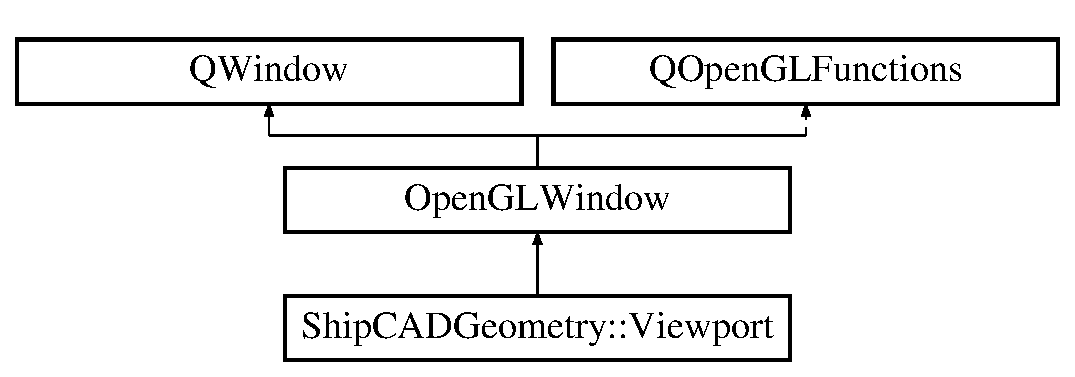
\includegraphics[height=3.000000cm]{classShipCADGeometry_1_1Viewport}
\end{center}
\end{figure}
\subsection*{Public Types}
\begin{DoxyCompactItemize}
\item 
enum \hyperlink{classShipCADGeometry_1_1Viewport_a32872391303d6fbcc5766df64933cc14}{viewport\-\_\-mode\-\_\-t} \{ \\*
\hyperlink{classShipCADGeometry_1_1Viewport_a32872391303d6fbcc5766df64933cc14aee736ccba0126663edb6080495acd9b6}{vm\-Wire\-Frame}, 
\hyperlink{classShipCADGeometry_1_1Viewport_a32872391303d6fbcc5766df64933cc14a9488ba3ad66c2b37b9406f0adbdd6792}{vm\-Shade}, 
\hyperlink{classShipCADGeometry_1_1Viewport_a32872391303d6fbcc5766df64933cc14a852f2c09b58295a234f0ee90eb47b9b8}{vm\-Shade\-Gauss}, 
\hyperlink{classShipCADGeometry_1_1Viewport_a32872391303d6fbcc5766df64933cc14a9da8a886df0e362400269f63b64482a9}{vm\-Shade\-Developable}, 
\\*
\hyperlink{classShipCADGeometry_1_1Viewport_a32872391303d6fbcc5766df64933cc14a8cb0ee8619f5beec0ee7a2b6cf906a22}{vm\-Shade\-Zebra}
 \}
\item 
enum \hyperlink{classShipCADGeometry_1_1Viewport_a97a32c07745357d09b8f282c69ea9199}{viewport\-\_\-type\-\_\-t} \{ \hyperlink{classShipCADGeometry_1_1Viewport_a97a32c07745357d09b8f282c69ea9199ac5dd44c84bae1db4b0e86b0aa6f43b6c}{fv\-Bodyplan}, 
\hyperlink{classShipCADGeometry_1_1Viewport_a97a32c07745357d09b8f282c69ea9199ae4c92b46bba3390a15ce065f040032fc}{fv\-Profile}, 
\hyperlink{classShipCADGeometry_1_1Viewport_a97a32c07745357d09b8f282c69ea9199affbe1a7334d2af879b3a7389728aa1d3}{fv\-Plan}, 
\hyperlink{classShipCADGeometry_1_1Viewport_a97a32c07745357d09b8f282c69ea9199a59cb7029a02145ca41c961ca4d4e363b}{fv\-Perspective}
 \}
\item 
enum \hyperlink{classShipCADGeometry_1_1Viewport_ae11090e9e924e7014fdff5111cb93810}{camera\-\_\-type\-\_\-t} \{ \\*
\hyperlink{classShipCADGeometry_1_1Viewport_ae11090e9e924e7014fdff5111cb93810afd29f18ed6bf8b4319c1115ba09dd784}{ft\-Wide}, 
\hyperlink{classShipCADGeometry_1_1Viewport_ae11090e9e924e7014fdff5111cb93810a446038d7865b3016be74c2d497cb920d}{ft\-Standard}, 
\hyperlink{classShipCADGeometry_1_1Viewport_ae11090e9e924e7014fdff5111cb93810a55510954d4c47518f04efa82ef32a02d}{ft\-Short\-Tele}, 
\hyperlink{classShipCADGeometry_1_1Viewport_ae11090e9e924e7014fdff5111cb93810a170fe6fb2532ac1196c9b8e863582907}{ft\-Medium\-Tele}, 
\\*
\hyperlink{classShipCADGeometry_1_1Viewport_ae11090e9e924e7014fdff5111cb93810a13236d349f46b99095decbaa4f6a2d9e}{ft\-Far\-Tele}
 \}
\end{DoxyCompactItemize}
\subsection*{Public Slots}
\begin{DoxyCompactItemize}
\item 
void \hyperlink{classShipCADGeometry_1_1Viewport_a578ac5ee96e36638739517fa21bf70c0}{set\-Viewport\-Mode} (\hyperlink{classShipCADGeometry_1_1Viewport_a32872391303d6fbcc5766df64933cc14}{viewport\-\_\-mode\-\_\-t} mode)
\item 
void \hyperlink{classShipCADGeometry_1_1Viewport_a554a3455c39ee5652b13c9b24c3c962e}{set\-Viewport\-Type} (\hyperlink{classShipCADGeometry_1_1Viewport_a97a32c07745357d09b8f282c69ea9199}{viewport\-\_\-type\-\_\-t} ty)
\item 
void \hyperlink{classShipCADGeometry_1_1Viewport_a5f90a885e0204b32ff9795c4b79f824b}{set\-Camera\-Type} (\hyperlink{classShipCADGeometry_1_1Viewport_ae11090e9e924e7014fdff5111cb93810}{camera\-\_\-type\-\_\-t} val)
\item 
void \hyperlink{classShipCADGeometry_1_1Viewport_a4bb2b85a12d7dd14e44b5d5c199cbda7}{set\-Surface} (\hyperlink{classShipCADGeometry_1_1SubdivisionSurface}{Subdivision\-Surface} $\ast$surface)
\item 
void \hyperlink{classShipCADGeometry_1_1Viewport_a00ba2139fa06701b65de70d5c657f5d6}{set\-Angle} (float val)
\item 
void \hyperlink{classShipCADGeometry_1_1Viewport_a4bda4b742dc477ed5dc2ab6ac7fe92bc}{set\-Elevation} (float val)
\item 
virtual void \hyperlink{classShipCADGeometry_1_1Viewport_a4eeeb100fd88487215bb7794bdf5e0cb}{resize\-Event} (Q\-Resize\-Event $\ast$\hyperlink{classOpenGLWindow_a1e3045cffb900de55b7384f5091c9d94}{event})
\end{DoxyCompactItemize}
\subsection*{Public Member Functions}
\begin{DoxyCompactItemize}
\item 
\hyperlink{classShipCADGeometry_1_1Viewport_a9fde8f966d9802dd42254acf0ed05386}{Viewport} ()
\item 
\hyperlink{classShipCADGeometry_1_1Viewport_a1e18a1ff4a52be33ef63d25034561850}{$\sim$\-Viewport} ()
\item 
void \hyperlink{classShipCADGeometry_1_1Viewport_a9c35de3f7c9d7c860c494081b48309b3}{initialize} ()
\item 
void \hyperlink{classShipCADGeometry_1_1Viewport_a9e81b526db3c2b508322c29b9fda5845}{render} ()
\item 
\hyperlink{classShipCADGeometry_1_1Viewport_a32872391303d6fbcc5766df64933cc14}{viewport\-\_\-mode\-\_\-t} \hyperlink{classShipCADGeometry_1_1Viewport_a3f5111023ade781b39ded6f4291e3a2f}{get\-Viewport\-Mode} () const 
\item 
\hyperlink{classShipCADGeometry_1_1Viewport_a97a32c07745357d09b8f282c69ea9199}{viewport\-\_\-type\-\_\-t} \hyperlink{classShipCADGeometry_1_1Viewport_ae11edc98f0eeae8adfaf7dec4f287f5f}{get\-Viewport\-Type} () const 
\item 
\hyperlink{classShipCADGeometry_1_1Viewport_ae11090e9e924e7014fdff5111cb93810}{camera\-\_\-type\-\_\-t} \hyperlink{classShipCADGeometry_1_1Viewport_ab589b68a7ad44e568d6b759d9af3aad5}{get\-Camera\-Type} () const 
\item 
\hyperlink{classShipCADGeometry_1_1SubdivisionSurface}{Subdivision\-Surface} $\ast$ \hyperlink{classShipCADGeometry_1_1Viewport_a9370f2d60910e34a90588e2db577c132}{get\-Surface} ()
\item 
void \hyperlink{classShipCADGeometry_1_1Viewport_a3626f44e62e08918de5939970cdc531c}{add} (\hyperlink{classShipCADGeometry_1_1Entity}{Entity} $\ast$entity)
\item 
void \hyperlink{classShipCADGeometry_1_1Viewport_a886ac5965b63039799827da89bf3de20}{add\-Shader} (const std\-::string \&name, \hyperlink{classShipCADGeometry_1_1Shader}{Shader} $\ast$shader)
\item 
\hyperlink{classShipCADGeometry_1_1LineShader}{Line\-Shader} $\ast$ \hyperlink{classShipCADGeometry_1_1Viewport_a0720a01f8650dc4acf89aad0649d9196}{set\-Line\-Shader} ()
\item 
\hyperlink{classShipCADGeometry_1_1MonoFaceShader}{Mono\-Face\-Shader} $\ast$ \hyperlink{classShipCADGeometry_1_1Viewport_a5f3c02f4e24d614d4340816d6de50b0b}{set\-Mono\-Face\-Shader} ()
\end{DoxyCompactItemize}
\subsection*{Protected Member Functions}
\begin{DoxyCompactItemize}
\item 
void \hyperlink{classShipCADGeometry_1_1Viewport_acef72369540d8e4d479eeadf5fdc3674}{initialize\-Viewport} (const Q\-Vector3\-D \&min, const Q\-Vector3\-D \&max)
\item 
void \hyperlink{classShipCADGeometry_1_1Viewport_a64a528202f47e6b10402f3aac161f85a}{convert\-Mouse\-Coord\-To\-World} (int mx, int my)
\item 
virtual void \hyperlink{classShipCADGeometry_1_1Viewport_a0dddc5b05c7308f8818a726b16a7d9eb}{mouse\-Press\-Event} (Q\-Mouse\-Event $\ast$)
\item 
virtual void \hyperlink{classShipCADGeometry_1_1Viewport_a7cb6994a92d40990b58be272953b9120}{mouse\-Release\-Event} (Q\-Mouse\-Event $\ast$)
\item 
virtual void \hyperlink{classShipCADGeometry_1_1Viewport_ab98dde7bb1d923b8cfc9a0c3cb249c2c}{mouse\-Move\-Event} (Q\-Mouse\-Event $\ast$)
\end{DoxyCompactItemize}


\subsection{Detailed Description}


Definition at line 50 of file viewport.\-h.



\subsection{Member Enumeration Documentation}
\hypertarget{classShipCADGeometry_1_1Viewport_ae11090e9e924e7014fdff5111cb93810}{\index{Ship\-C\-A\-D\-Geometry\-::\-Viewport@{Ship\-C\-A\-D\-Geometry\-::\-Viewport}!camera\-\_\-type\-\_\-t@{camera\-\_\-type\-\_\-t}}
\index{camera\-\_\-type\-\_\-t@{camera\-\_\-type\-\_\-t}!ShipCADGeometry::Viewport@{Ship\-C\-A\-D\-Geometry\-::\-Viewport}}
\subsubsection[{camera\-\_\-type\-\_\-t}]{\setlength{\rightskip}{0pt plus 5cm}enum {\bf Ship\-C\-A\-D\-Geometry\-::\-Viewport\-::camera\-\_\-type\-\_\-t}}}\label{classShipCADGeometry_1_1Viewport_ae11090e9e924e7014fdff5111cb93810}
\begin{Desc}
\item[Enumerator]\par
\begin{description}
\index{ft\-Wide@{ft\-Wide}!Ship\-C\-A\-D\-Geometry\-::\-Viewport@{Ship\-C\-A\-D\-Geometry\-::\-Viewport}}\index{Ship\-C\-A\-D\-Geometry\-::\-Viewport@{Ship\-C\-A\-D\-Geometry\-::\-Viewport}!ft\-Wide@{ft\-Wide}}\item[{\em 
\hypertarget{classShipCADGeometry_1_1Viewport_ae11090e9e924e7014fdff5111cb93810afd29f18ed6bf8b4319c1115ba09dd784}{ft\-Wide}\label{classShipCADGeometry_1_1Viewport_ae11090e9e924e7014fdff5111cb93810afd29f18ed6bf8b4319c1115ba09dd784}
}]\index{ft\-Standard@{ft\-Standard}!Ship\-C\-A\-D\-Geometry\-::\-Viewport@{Ship\-C\-A\-D\-Geometry\-::\-Viewport}}\index{Ship\-C\-A\-D\-Geometry\-::\-Viewport@{Ship\-C\-A\-D\-Geometry\-::\-Viewport}!ft\-Standard@{ft\-Standard}}\item[{\em 
\hypertarget{classShipCADGeometry_1_1Viewport_ae11090e9e924e7014fdff5111cb93810a446038d7865b3016be74c2d497cb920d}{ft\-Standard}\label{classShipCADGeometry_1_1Viewport_ae11090e9e924e7014fdff5111cb93810a446038d7865b3016be74c2d497cb920d}
}]\index{ft\-Short\-Tele@{ft\-Short\-Tele}!Ship\-C\-A\-D\-Geometry\-::\-Viewport@{Ship\-C\-A\-D\-Geometry\-::\-Viewport}}\index{Ship\-C\-A\-D\-Geometry\-::\-Viewport@{Ship\-C\-A\-D\-Geometry\-::\-Viewport}!ft\-Short\-Tele@{ft\-Short\-Tele}}\item[{\em 
\hypertarget{classShipCADGeometry_1_1Viewport_ae11090e9e924e7014fdff5111cb93810a55510954d4c47518f04efa82ef32a02d}{ft\-Short\-Tele}\label{classShipCADGeometry_1_1Viewport_ae11090e9e924e7014fdff5111cb93810a55510954d4c47518f04efa82ef32a02d}
}]\index{ft\-Medium\-Tele@{ft\-Medium\-Tele}!Ship\-C\-A\-D\-Geometry\-::\-Viewport@{Ship\-C\-A\-D\-Geometry\-::\-Viewport}}\index{Ship\-C\-A\-D\-Geometry\-::\-Viewport@{Ship\-C\-A\-D\-Geometry\-::\-Viewport}!ft\-Medium\-Tele@{ft\-Medium\-Tele}}\item[{\em 
\hypertarget{classShipCADGeometry_1_1Viewport_ae11090e9e924e7014fdff5111cb93810a170fe6fb2532ac1196c9b8e863582907}{ft\-Medium\-Tele}\label{classShipCADGeometry_1_1Viewport_ae11090e9e924e7014fdff5111cb93810a170fe6fb2532ac1196c9b8e863582907}
}]\index{ft\-Far\-Tele@{ft\-Far\-Tele}!Ship\-C\-A\-D\-Geometry\-::\-Viewport@{Ship\-C\-A\-D\-Geometry\-::\-Viewport}}\index{Ship\-C\-A\-D\-Geometry\-::\-Viewport@{Ship\-C\-A\-D\-Geometry\-::\-Viewport}!ft\-Far\-Tele@{ft\-Far\-Tele}}\item[{\em 
\hypertarget{classShipCADGeometry_1_1Viewport_ae11090e9e924e7014fdff5111cb93810a13236d349f46b99095decbaa4f6a2d9e}{ft\-Far\-Tele}\label{classShipCADGeometry_1_1Viewport_ae11090e9e924e7014fdff5111cb93810a13236d349f46b99095decbaa4f6a2d9e}
}]\end{description}
\end{Desc}


Definition at line 64 of file viewport.\-h.

\hypertarget{classShipCADGeometry_1_1Viewport_a32872391303d6fbcc5766df64933cc14}{\index{Ship\-C\-A\-D\-Geometry\-::\-Viewport@{Ship\-C\-A\-D\-Geometry\-::\-Viewport}!viewport\-\_\-mode\-\_\-t@{viewport\-\_\-mode\-\_\-t}}
\index{viewport\-\_\-mode\-\_\-t@{viewport\-\_\-mode\-\_\-t}!ShipCADGeometry::Viewport@{Ship\-C\-A\-D\-Geometry\-::\-Viewport}}
\subsubsection[{viewport\-\_\-mode\-\_\-t}]{\setlength{\rightskip}{0pt plus 5cm}enum {\bf Ship\-C\-A\-D\-Geometry\-::\-Viewport\-::viewport\-\_\-mode\-\_\-t}}}\label{classShipCADGeometry_1_1Viewport_a32872391303d6fbcc5766df64933cc14}
\begin{Desc}
\item[Enumerator]\par
\begin{description}
\index{vm\-Wire\-Frame@{vm\-Wire\-Frame}!Ship\-C\-A\-D\-Geometry\-::\-Viewport@{Ship\-C\-A\-D\-Geometry\-::\-Viewport}}\index{Ship\-C\-A\-D\-Geometry\-::\-Viewport@{Ship\-C\-A\-D\-Geometry\-::\-Viewport}!vm\-Wire\-Frame@{vm\-Wire\-Frame}}\item[{\em 
\hypertarget{classShipCADGeometry_1_1Viewport_a32872391303d6fbcc5766df64933cc14aee736ccba0126663edb6080495acd9b6}{vm\-Wire\-Frame}\label{classShipCADGeometry_1_1Viewport_a32872391303d6fbcc5766df64933cc14aee736ccba0126663edb6080495acd9b6}
}]\index{vm\-Shade@{vm\-Shade}!Ship\-C\-A\-D\-Geometry\-::\-Viewport@{Ship\-C\-A\-D\-Geometry\-::\-Viewport}}\index{Ship\-C\-A\-D\-Geometry\-::\-Viewport@{Ship\-C\-A\-D\-Geometry\-::\-Viewport}!vm\-Shade@{vm\-Shade}}\item[{\em 
\hypertarget{classShipCADGeometry_1_1Viewport_a32872391303d6fbcc5766df64933cc14a9488ba3ad66c2b37b9406f0adbdd6792}{vm\-Shade}\label{classShipCADGeometry_1_1Viewport_a32872391303d6fbcc5766df64933cc14a9488ba3ad66c2b37b9406f0adbdd6792}
}]\index{vm\-Shade\-Gauss@{vm\-Shade\-Gauss}!Ship\-C\-A\-D\-Geometry\-::\-Viewport@{Ship\-C\-A\-D\-Geometry\-::\-Viewport}}\index{Ship\-C\-A\-D\-Geometry\-::\-Viewport@{Ship\-C\-A\-D\-Geometry\-::\-Viewport}!vm\-Shade\-Gauss@{vm\-Shade\-Gauss}}\item[{\em 
\hypertarget{classShipCADGeometry_1_1Viewport_a32872391303d6fbcc5766df64933cc14a852f2c09b58295a234f0ee90eb47b9b8}{vm\-Shade\-Gauss}\label{classShipCADGeometry_1_1Viewport_a32872391303d6fbcc5766df64933cc14a852f2c09b58295a234f0ee90eb47b9b8}
}]\index{vm\-Shade\-Developable@{vm\-Shade\-Developable}!Ship\-C\-A\-D\-Geometry\-::\-Viewport@{Ship\-C\-A\-D\-Geometry\-::\-Viewport}}\index{Ship\-C\-A\-D\-Geometry\-::\-Viewport@{Ship\-C\-A\-D\-Geometry\-::\-Viewport}!vm\-Shade\-Developable@{vm\-Shade\-Developable}}\item[{\em 
\hypertarget{classShipCADGeometry_1_1Viewport_a32872391303d6fbcc5766df64933cc14a9da8a886df0e362400269f63b64482a9}{vm\-Shade\-Developable}\label{classShipCADGeometry_1_1Viewport_a32872391303d6fbcc5766df64933cc14a9da8a886df0e362400269f63b64482a9}
}]\index{vm\-Shade\-Zebra@{vm\-Shade\-Zebra}!Ship\-C\-A\-D\-Geometry\-::\-Viewport@{Ship\-C\-A\-D\-Geometry\-::\-Viewport}}\index{Ship\-C\-A\-D\-Geometry\-::\-Viewport@{Ship\-C\-A\-D\-Geometry\-::\-Viewport}!vm\-Shade\-Zebra@{vm\-Shade\-Zebra}}\item[{\em 
\hypertarget{classShipCADGeometry_1_1Viewport_a32872391303d6fbcc5766df64933cc14a8cb0ee8619f5beec0ee7a2b6cf906a22}{vm\-Shade\-Zebra}\label{classShipCADGeometry_1_1Viewport_a32872391303d6fbcc5766df64933cc14a8cb0ee8619f5beec0ee7a2b6cf906a22}
}]\end{description}
\end{Desc}


Definition at line 58 of file viewport.\-h.

\hypertarget{classShipCADGeometry_1_1Viewport_a97a32c07745357d09b8f282c69ea9199}{\index{Ship\-C\-A\-D\-Geometry\-::\-Viewport@{Ship\-C\-A\-D\-Geometry\-::\-Viewport}!viewport\-\_\-type\-\_\-t@{viewport\-\_\-type\-\_\-t}}
\index{viewport\-\_\-type\-\_\-t@{viewport\-\_\-type\-\_\-t}!ShipCADGeometry::Viewport@{Ship\-C\-A\-D\-Geometry\-::\-Viewport}}
\subsubsection[{viewport\-\_\-type\-\_\-t}]{\setlength{\rightskip}{0pt plus 5cm}enum {\bf Ship\-C\-A\-D\-Geometry\-::\-Viewport\-::viewport\-\_\-type\-\_\-t}}}\label{classShipCADGeometry_1_1Viewport_a97a32c07745357d09b8f282c69ea9199}
\begin{Desc}
\item[Enumerator]\par
\begin{description}
\index{fv\-Bodyplan@{fv\-Bodyplan}!Ship\-C\-A\-D\-Geometry\-::\-Viewport@{Ship\-C\-A\-D\-Geometry\-::\-Viewport}}\index{Ship\-C\-A\-D\-Geometry\-::\-Viewport@{Ship\-C\-A\-D\-Geometry\-::\-Viewport}!fv\-Bodyplan@{fv\-Bodyplan}}\item[{\em 
\hypertarget{classShipCADGeometry_1_1Viewport_a97a32c07745357d09b8f282c69ea9199ac5dd44c84bae1db4b0e86b0aa6f43b6c}{fv\-Bodyplan}\label{classShipCADGeometry_1_1Viewport_a97a32c07745357d09b8f282c69ea9199ac5dd44c84bae1db4b0e86b0aa6f43b6c}
}]\index{fv\-Profile@{fv\-Profile}!Ship\-C\-A\-D\-Geometry\-::\-Viewport@{Ship\-C\-A\-D\-Geometry\-::\-Viewport}}\index{Ship\-C\-A\-D\-Geometry\-::\-Viewport@{Ship\-C\-A\-D\-Geometry\-::\-Viewport}!fv\-Profile@{fv\-Profile}}\item[{\em 
\hypertarget{classShipCADGeometry_1_1Viewport_a97a32c07745357d09b8f282c69ea9199ae4c92b46bba3390a15ce065f040032fc}{fv\-Profile}\label{classShipCADGeometry_1_1Viewport_a97a32c07745357d09b8f282c69ea9199ae4c92b46bba3390a15ce065f040032fc}
}]\index{fv\-Plan@{fv\-Plan}!Ship\-C\-A\-D\-Geometry\-::\-Viewport@{Ship\-C\-A\-D\-Geometry\-::\-Viewport}}\index{Ship\-C\-A\-D\-Geometry\-::\-Viewport@{Ship\-C\-A\-D\-Geometry\-::\-Viewport}!fv\-Plan@{fv\-Plan}}\item[{\em 
\hypertarget{classShipCADGeometry_1_1Viewport_a97a32c07745357d09b8f282c69ea9199affbe1a7334d2af879b3a7389728aa1d3}{fv\-Plan}\label{classShipCADGeometry_1_1Viewport_a97a32c07745357d09b8f282c69ea9199affbe1a7334d2af879b3a7389728aa1d3}
}]\index{fv\-Perspective@{fv\-Perspective}!Ship\-C\-A\-D\-Geometry\-::\-Viewport@{Ship\-C\-A\-D\-Geometry\-::\-Viewport}}\index{Ship\-C\-A\-D\-Geometry\-::\-Viewport@{Ship\-C\-A\-D\-Geometry\-::\-Viewport}!fv\-Perspective@{fv\-Perspective}}\item[{\em 
\hypertarget{classShipCADGeometry_1_1Viewport_a97a32c07745357d09b8f282c69ea9199a59cb7029a02145ca41c961ca4d4e363b}{fv\-Perspective}\label{classShipCADGeometry_1_1Viewport_a97a32c07745357d09b8f282c69ea9199a59cb7029a02145ca41c961ca4d4e363b}
}]\end{description}
\end{Desc}


Definition at line 61 of file viewport.\-h.



\subsection{Constructor \& Destructor Documentation}
\hypertarget{classShipCADGeometry_1_1Viewport_a9fde8f966d9802dd42254acf0ed05386}{\index{Ship\-C\-A\-D\-Geometry\-::\-Viewport@{Ship\-C\-A\-D\-Geometry\-::\-Viewport}!Viewport@{Viewport}}
\index{Viewport@{Viewport}!ShipCADGeometry::Viewport@{Ship\-C\-A\-D\-Geometry\-::\-Viewport}}
\subsubsection[{Viewport}]{\setlength{\rightskip}{0pt plus 5cm}Viewport\-::\-Viewport (
\begin{DoxyParamCaption}
{}
\end{DoxyParamCaption}
)\hspace{0.3cm}{\ttfamily [explicit]}}}\label{classShipCADGeometry_1_1Viewport_a9fde8f966d9802dd42254acf0ed05386}


Definition at line 42 of file viewport.\-cpp.

\hypertarget{classShipCADGeometry_1_1Viewport_a1e18a1ff4a52be33ef63d25034561850}{\index{Ship\-C\-A\-D\-Geometry\-::\-Viewport@{Ship\-C\-A\-D\-Geometry\-::\-Viewport}!$\sim$\-Viewport@{$\sim$\-Viewport}}
\index{$\sim$\-Viewport@{$\sim$\-Viewport}!ShipCADGeometry::Viewport@{Ship\-C\-A\-D\-Geometry\-::\-Viewport}}
\subsubsection[{$\sim$\-Viewport}]{\setlength{\rightskip}{0pt plus 5cm}Viewport\-::$\sim$\-Viewport (
\begin{DoxyParamCaption}
{}
\end{DoxyParamCaption}
)}}\label{classShipCADGeometry_1_1Viewport_a1e18a1ff4a52be33ef63d25034561850}


Definition at line 54 of file viewport.\-cpp.



\subsection{Member Function Documentation}
\hypertarget{classShipCADGeometry_1_1Viewport_a3626f44e62e08918de5939970cdc531c}{\index{Ship\-C\-A\-D\-Geometry\-::\-Viewport@{Ship\-C\-A\-D\-Geometry\-::\-Viewport}!add@{add}}
\index{add@{add}!ShipCADGeometry::Viewport@{Ship\-C\-A\-D\-Geometry\-::\-Viewport}}
\subsubsection[{add}]{\setlength{\rightskip}{0pt plus 5cm}void Viewport\-::add (
\begin{DoxyParamCaption}
\item[{{\bf Entity} $\ast$}]{entity}
\end{DoxyParamCaption}
)}}\label{classShipCADGeometry_1_1Viewport_a3626f44e62e08918de5939970cdc531c}


Definition at line 202 of file viewport.\-cpp.

\hypertarget{classShipCADGeometry_1_1Viewport_a886ac5965b63039799827da89bf3de20}{\index{Ship\-C\-A\-D\-Geometry\-::\-Viewport@{Ship\-C\-A\-D\-Geometry\-::\-Viewport}!add\-Shader@{add\-Shader}}
\index{add\-Shader@{add\-Shader}!ShipCADGeometry::Viewport@{Ship\-C\-A\-D\-Geometry\-::\-Viewport}}
\subsubsection[{add\-Shader}]{\setlength{\rightskip}{0pt plus 5cm}void Viewport\-::add\-Shader (
\begin{DoxyParamCaption}
\item[{const std\-::string \&}]{name, }
\item[{{\bf Shader} $\ast$}]{shader}
\end{DoxyParamCaption}
)}}\label{classShipCADGeometry_1_1Viewport_a886ac5965b63039799827da89bf3de20}


Definition at line 222 of file viewport.\-cpp.

\hypertarget{classShipCADGeometry_1_1Viewport_a64a528202f47e6b10402f3aac161f85a}{\index{Ship\-C\-A\-D\-Geometry\-::\-Viewport@{Ship\-C\-A\-D\-Geometry\-::\-Viewport}!convert\-Mouse\-Coord\-To\-World@{convert\-Mouse\-Coord\-To\-World}}
\index{convert\-Mouse\-Coord\-To\-World@{convert\-Mouse\-Coord\-To\-World}!ShipCADGeometry::Viewport@{Ship\-C\-A\-D\-Geometry\-::\-Viewport}}
\subsubsection[{convert\-Mouse\-Coord\-To\-World}]{\setlength{\rightskip}{0pt plus 5cm}void Viewport\-::convert\-Mouse\-Coord\-To\-World (
\begin{DoxyParamCaption}
\item[{int}]{mx, }
\item[{int}]{my}
\end{DoxyParamCaption}
)\hspace{0.3cm}{\ttfamily [protected]}}}\label{classShipCADGeometry_1_1Viewport_a64a528202f47e6b10402f3aac161f85a}


Definition at line 276 of file viewport.\-cpp.

\hypertarget{classShipCADGeometry_1_1Viewport_ab589b68a7ad44e568d6b759d9af3aad5}{\index{Ship\-C\-A\-D\-Geometry\-::\-Viewport@{Ship\-C\-A\-D\-Geometry\-::\-Viewport}!get\-Camera\-Type@{get\-Camera\-Type}}
\index{get\-Camera\-Type@{get\-Camera\-Type}!ShipCADGeometry::Viewport@{Ship\-C\-A\-D\-Geometry\-::\-Viewport}}
\subsubsection[{get\-Camera\-Type}]{\setlength{\rightskip}{0pt plus 5cm}{\bf camera\-\_\-type\-\_\-t} Ship\-C\-A\-D\-Geometry\-::\-Viewport\-::get\-Camera\-Type (
\begin{DoxyParamCaption}
{}
\end{DoxyParamCaption}
) const\hspace{0.3cm}{\ttfamily [inline]}}}\label{classShipCADGeometry_1_1Viewport_ab589b68a7ad44e568d6b759d9af3aad5}


Definition at line 75 of file viewport.\-h.

\hypertarget{classShipCADGeometry_1_1Viewport_a9370f2d60910e34a90588e2db577c132}{\index{Ship\-C\-A\-D\-Geometry\-::\-Viewport@{Ship\-C\-A\-D\-Geometry\-::\-Viewport}!get\-Surface@{get\-Surface}}
\index{get\-Surface@{get\-Surface}!ShipCADGeometry::Viewport@{Ship\-C\-A\-D\-Geometry\-::\-Viewport}}
\subsubsection[{get\-Surface}]{\setlength{\rightskip}{0pt plus 5cm}{\bf Subdivision\-Surface}$\ast$ Ship\-C\-A\-D\-Geometry\-::\-Viewport\-::get\-Surface (
\begin{DoxyParamCaption}
{}
\end{DoxyParamCaption}
)\hspace{0.3cm}{\ttfamily [inline]}}}\label{classShipCADGeometry_1_1Viewport_a9370f2d60910e34a90588e2db577c132}


Definition at line 77 of file viewport.\-h.

\hypertarget{classShipCADGeometry_1_1Viewport_a3f5111023ade781b39ded6f4291e3a2f}{\index{Ship\-C\-A\-D\-Geometry\-::\-Viewport@{Ship\-C\-A\-D\-Geometry\-::\-Viewport}!get\-Viewport\-Mode@{get\-Viewport\-Mode}}
\index{get\-Viewport\-Mode@{get\-Viewport\-Mode}!ShipCADGeometry::Viewport@{Ship\-C\-A\-D\-Geometry\-::\-Viewport}}
\subsubsection[{get\-Viewport\-Mode}]{\setlength{\rightskip}{0pt plus 5cm}{\bf viewport\-\_\-mode\-\_\-t} Ship\-C\-A\-D\-Geometry\-::\-Viewport\-::get\-Viewport\-Mode (
\begin{DoxyParamCaption}
{}
\end{DoxyParamCaption}
) const\hspace{0.3cm}{\ttfamily [inline]}}}\label{classShipCADGeometry_1_1Viewport_a3f5111023ade781b39ded6f4291e3a2f}


Definition at line 71 of file viewport.\-h.

\hypertarget{classShipCADGeometry_1_1Viewport_ae11edc98f0eeae8adfaf7dec4f287f5f}{\index{Ship\-C\-A\-D\-Geometry\-::\-Viewport@{Ship\-C\-A\-D\-Geometry\-::\-Viewport}!get\-Viewport\-Type@{get\-Viewport\-Type}}
\index{get\-Viewport\-Type@{get\-Viewport\-Type}!ShipCADGeometry::Viewport@{Ship\-C\-A\-D\-Geometry\-::\-Viewport}}
\subsubsection[{get\-Viewport\-Type}]{\setlength{\rightskip}{0pt plus 5cm}{\bf viewport\-\_\-type\-\_\-t} Ship\-C\-A\-D\-Geometry\-::\-Viewport\-::get\-Viewport\-Type (
\begin{DoxyParamCaption}
{}
\end{DoxyParamCaption}
) const\hspace{0.3cm}{\ttfamily [inline]}}}\label{classShipCADGeometry_1_1Viewport_ae11edc98f0eeae8adfaf7dec4f287f5f}


Definition at line 73 of file viewport.\-h.

\hypertarget{classShipCADGeometry_1_1Viewport_a9c35de3f7c9d7c860c494081b48309b3}{\index{Ship\-C\-A\-D\-Geometry\-::\-Viewport@{Ship\-C\-A\-D\-Geometry\-::\-Viewport}!initialize@{initialize}}
\index{initialize@{initialize}!ShipCADGeometry::Viewport@{Ship\-C\-A\-D\-Geometry\-::\-Viewport}}
\subsubsection[{initialize}]{\setlength{\rightskip}{0pt plus 5cm}void Viewport\-::initialize (
\begin{DoxyParamCaption}
{}
\end{DoxyParamCaption}
)\hspace{0.3cm}{\ttfamily [virtual]}}}\label{classShipCADGeometry_1_1Viewport_a9c35de3f7c9d7c860c494081b48309b3}


Reimplemented from \hyperlink{classOpenGLWindow_aed4e2ee22e113b2f7e7d1eba4ef1b965}{Open\-G\-L\-Window}.



Definition at line 63 of file viewport.\-cpp.

\hypertarget{classShipCADGeometry_1_1Viewport_acef72369540d8e4d479eeadf5fdc3674}{\index{Ship\-C\-A\-D\-Geometry\-::\-Viewport@{Ship\-C\-A\-D\-Geometry\-::\-Viewport}!initialize\-Viewport@{initialize\-Viewport}}
\index{initialize\-Viewport@{initialize\-Viewport}!ShipCADGeometry::Viewport@{Ship\-C\-A\-D\-Geometry\-::\-Viewport}}
\subsubsection[{initialize\-Viewport}]{\setlength{\rightskip}{0pt plus 5cm}void Viewport\-::initialize\-Viewport (
\begin{DoxyParamCaption}
\item[{const Q\-Vector3\-D \&}]{min, }
\item[{const Q\-Vector3\-D \&}]{max}
\end{DoxyParamCaption}
)\hspace{0.3cm}{\ttfamily [protected]}}}\label{classShipCADGeometry_1_1Viewport_acef72369540d8e4d479eeadf5fdc3674}


Definition at line 155 of file viewport.\-cpp.

\hypertarget{classShipCADGeometry_1_1Viewport_ab98dde7bb1d923b8cfc9a0c3cb249c2c}{\index{Ship\-C\-A\-D\-Geometry\-::\-Viewport@{Ship\-C\-A\-D\-Geometry\-::\-Viewport}!mouse\-Move\-Event@{mouse\-Move\-Event}}
\index{mouse\-Move\-Event@{mouse\-Move\-Event}!ShipCADGeometry::Viewport@{Ship\-C\-A\-D\-Geometry\-::\-Viewport}}
\subsubsection[{mouse\-Move\-Event}]{\setlength{\rightskip}{0pt plus 5cm}void Viewport\-::mouse\-Move\-Event (
\begin{DoxyParamCaption}
\item[{Q\-Mouse\-Event $\ast$}]{event}
\end{DoxyParamCaption}
)\hspace{0.3cm}{\ttfamily [protected]}, {\ttfamily [virtual]}}}\label{classShipCADGeometry_1_1Viewport_ab98dde7bb1d923b8cfc9a0c3cb249c2c}


Definition at line 337 of file viewport.\-cpp.

\hypertarget{classShipCADGeometry_1_1Viewport_a0dddc5b05c7308f8818a726b16a7d9eb}{\index{Ship\-C\-A\-D\-Geometry\-::\-Viewport@{Ship\-C\-A\-D\-Geometry\-::\-Viewport}!mouse\-Press\-Event@{mouse\-Press\-Event}}
\index{mouse\-Press\-Event@{mouse\-Press\-Event}!ShipCADGeometry::Viewport@{Ship\-C\-A\-D\-Geometry\-::\-Viewport}}
\subsubsection[{mouse\-Press\-Event}]{\setlength{\rightskip}{0pt plus 5cm}void Viewport\-::mouse\-Press\-Event (
\begin{DoxyParamCaption}
\item[{Q\-Mouse\-Event $\ast$}]{event}
\end{DoxyParamCaption}
)\hspace{0.3cm}{\ttfamily [protected]}, {\ttfamily [virtual]}}}\label{classShipCADGeometry_1_1Viewport_a0dddc5b05c7308f8818a726b16a7d9eb}


Definition at line 316 of file viewport.\-cpp.

\hypertarget{classShipCADGeometry_1_1Viewport_a7cb6994a92d40990b58be272953b9120}{\index{Ship\-C\-A\-D\-Geometry\-::\-Viewport@{Ship\-C\-A\-D\-Geometry\-::\-Viewport}!mouse\-Release\-Event@{mouse\-Release\-Event}}
\index{mouse\-Release\-Event@{mouse\-Release\-Event}!ShipCADGeometry::Viewport@{Ship\-C\-A\-D\-Geometry\-::\-Viewport}}
\subsubsection[{mouse\-Release\-Event}]{\setlength{\rightskip}{0pt plus 5cm}void Viewport\-::mouse\-Release\-Event (
\begin{DoxyParamCaption}
\item[{Q\-Mouse\-Event $\ast$}]{event}
\end{DoxyParamCaption}
)\hspace{0.3cm}{\ttfamily [protected]}, {\ttfamily [virtual]}}}\label{classShipCADGeometry_1_1Viewport_a7cb6994a92d40990b58be272953b9120}


Definition at line 325 of file viewport.\-cpp.

\hypertarget{classShipCADGeometry_1_1Viewport_a9e81b526db3c2b508322c29b9fda5845}{\index{Ship\-C\-A\-D\-Geometry\-::\-Viewport@{Ship\-C\-A\-D\-Geometry\-::\-Viewport}!render@{render}}
\index{render@{render}!ShipCADGeometry::Viewport@{Ship\-C\-A\-D\-Geometry\-::\-Viewport}}
\subsubsection[{render}]{\setlength{\rightskip}{0pt plus 5cm}void Viewport\-::render (
\begin{DoxyParamCaption}
{}
\end{DoxyParamCaption}
)\hspace{0.3cm}{\ttfamily [virtual]}}}\label{classShipCADGeometry_1_1Viewport_a9e81b526db3c2b508322c29b9fda5845}


Reimplemented from \hyperlink{classOpenGLWindow_ac9e094864803a0b29364f42c2a47fa8c}{Open\-G\-L\-Window}.



Definition at line 227 of file viewport.\-cpp.

\hypertarget{classShipCADGeometry_1_1Viewport_a4eeeb100fd88487215bb7794bdf5e0cb}{\index{Ship\-C\-A\-D\-Geometry\-::\-Viewport@{Ship\-C\-A\-D\-Geometry\-::\-Viewport}!resize\-Event@{resize\-Event}}
\index{resize\-Event@{resize\-Event}!ShipCADGeometry::Viewport@{Ship\-C\-A\-D\-Geometry\-::\-Viewport}}
\subsubsection[{resize\-Event}]{\setlength{\rightskip}{0pt plus 5cm}void Viewport\-::resize\-Event (
\begin{DoxyParamCaption}
\item[{Q\-Resize\-Event $\ast$}]{event}
\end{DoxyParamCaption}
)\hspace{0.3cm}{\ttfamily [virtual]}, {\ttfamily [slot]}}}\label{classShipCADGeometry_1_1Viewport_a4eeeb100fd88487215bb7794bdf5e0cb}


Definition at line 146 of file viewport.\-cpp.

\hypertarget{classShipCADGeometry_1_1Viewport_a00ba2139fa06701b65de70d5c657f5d6}{\index{Ship\-C\-A\-D\-Geometry\-::\-Viewport@{Ship\-C\-A\-D\-Geometry\-::\-Viewport}!set\-Angle@{set\-Angle}}
\index{set\-Angle@{set\-Angle}!ShipCADGeometry::Viewport@{Ship\-C\-A\-D\-Geometry\-::\-Viewport}}
\subsubsection[{set\-Angle}]{\setlength{\rightskip}{0pt plus 5cm}void Viewport\-::set\-Angle (
\begin{DoxyParamCaption}
\item[{float}]{val}
\end{DoxyParamCaption}
)\hspace{0.3cm}{\ttfamily [slot]}}}\label{classShipCADGeometry_1_1Viewport_a00ba2139fa06701b65de70d5c657f5d6}


Definition at line 130 of file viewport.\-cpp.

\hypertarget{classShipCADGeometry_1_1Viewport_a5f90a885e0204b32ff9795c4b79f824b}{\index{Ship\-C\-A\-D\-Geometry\-::\-Viewport@{Ship\-C\-A\-D\-Geometry\-::\-Viewport}!set\-Camera\-Type@{set\-Camera\-Type}}
\index{set\-Camera\-Type@{set\-Camera\-Type}!ShipCADGeometry::Viewport@{Ship\-C\-A\-D\-Geometry\-::\-Viewport}}
\subsubsection[{set\-Camera\-Type}]{\setlength{\rightskip}{0pt plus 5cm}void Viewport\-::set\-Camera\-Type (
\begin{DoxyParamCaption}
\item[{{\bf camera\-\_\-type\-\_\-t}}]{val}
\end{DoxyParamCaption}
)\hspace{0.3cm}{\ttfamily [slot]}}}\label{classShipCADGeometry_1_1Viewport_a5f90a885e0204b32ff9795c4b79f824b}


Definition at line 78 of file viewport.\-cpp.

\hypertarget{classShipCADGeometry_1_1Viewport_a4bda4b742dc477ed5dc2ab6ac7fe92bc}{\index{Ship\-C\-A\-D\-Geometry\-::\-Viewport@{Ship\-C\-A\-D\-Geometry\-::\-Viewport}!set\-Elevation@{set\-Elevation}}
\index{set\-Elevation@{set\-Elevation}!ShipCADGeometry::Viewport@{Ship\-C\-A\-D\-Geometry\-::\-Viewport}}
\subsubsection[{set\-Elevation}]{\setlength{\rightskip}{0pt plus 5cm}void Viewport\-::set\-Elevation (
\begin{DoxyParamCaption}
\item[{float}]{val}
\end{DoxyParamCaption}
)\hspace{0.3cm}{\ttfamily [slot]}}}\label{classShipCADGeometry_1_1Viewport_a4bda4b742dc477ed5dc2ab6ac7fe92bc}


Definition at line 138 of file viewport.\-cpp.

\hypertarget{classShipCADGeometry_1_1Viewport_a0720a01f8650dc4acf89aad0649d9196}{\index{Ship\-C\-A\-D\-Geometry\-::\-Viewport@{Ship\-C\-A\-D\-Geometry\-::\-Viewport}!set\-Line\-Shader@{set\-Line\-Shader}}
\index{set\-Line\-Shader@{set\-Line\-Shader}!ShipCADGeometry::Viewport@{Ship\-C\-A\-D\-Geometry\-::\-Viewport}}
\subsubsection[{set\-Line\-Shader}]{\setlength{\rightskip}{0pt plus 5cm}{\bf Line\-Shader} $\ast$ Viewport\-::set\-Line\-Shader (
\begin{DoxyParamCaption}
{}
\end{DoxyParamCaption}
)}}\label{classShipCADGeometry_1_1Viewport_a0720a01f8650dc4acf89aad0649d9196}


Definition at line 247 of file viewport.\-cpp.

\hypertarget{classShipCADGeometry_1_1Viewport_a5f3c02f4e24d614d4340816d6de50b0b}{\index{Ship\-C\-A\-D\-Geometry\-::\-Viewport@{Ship\-C\-A\-D\-Geometry\-::\-Viewport}!set\-Mono\-Face\-Shader@{set\-Mono\-Face\-Shader}}
\index{set\-Mono\-Face\-Shader@{set\-Mono\-Face\-Shader}!ShipCADGeometry::Viewport@{Ship\-C\-A\-D\-Geometry\-::\-Viewport}}
\subsubsection[{set\-Mono\-Face\-Shader}]{\setlength{\rightskip}{0pt plus 5cm}{\bf Mono\-Face\-Shader} $\ast$ Viewport\-::set\-Mono\-Face\-Shader (
\begin{DoxyParamCaption}
{}
\end{DoxyParamCaption}
)}}\label{classShipCADGeometry_1_1Viewport_a5f3c02f4e24d614d4340816d6de50b0b}


Definition at line 261 of file viewport.\-cpp.

\hypertarget{classShipCADGeometry_1_1Viewport_a4bb2b85a12d7dd14e44b5d5c199cbda7}{\index{Ship\-C\-A\-D\-Geometry\-::\-Viewport@{Ship\-C\-A\-D\-Geometry\-::\-Viewport}!set\-Surface@{set\-Surface}}
\index{set\-Surface@{set\-Surface}!ShipCADGeometry::Viewport@{Ship\-C\-A\-D\-Geometry\-::\-Viewport}}
\subsubsection[{set\-Surface}]{\setlength{\rightskip}{0pt plus 5cm}void Viewport\-::set\-Surface (
\begin{DoxyParamCaption}
\item[{{\bf Subdivision\-Surface} $\ast$}]{surface}
\end{DoxyParamCaption}
)\hspace{0.3cm}{\ttfamily [slot]}}}\label{classShipCADGeometry_1_1Viewport_a4bb2b85a12d7dd14e44b5d5c199cbda7}


Definition at line 207 of file viewport.\-cpp.

\hypertarget{classShipCADGeometry_1_1Viewport_a578ac5ee96e36638739517fa21bf70c0}{\index{Ship\-C\-A\-D\-Geometry\-::\-Viewport@{Ship\-C\-A\-D\-Geometry\-::\-Viewport}!set\-Viewport\-Mode@{set\-Viewport\-Mode}}
\index{set\-Viewport\-Mode@{set\-Viewport\-Mode}!ShipCADGeometry::Viewport@{Ship\-C\-A\-D\-Geometry\-::\-Viewport}}
\subsubsection[{set\-Viewport\-Mode}]{\setlength{\rightskip}{0pt plus 5cm}void Viewport\-::set\-Viewport\-Mode (
\begin{DoxyParamCaption}
\item[{{\bf viewport\-\_\-mode\-\_\-t}}]{mode}
\end{DoxyParamCaption}
)\hspace{0.3cm}{\ttfamily [slot]}}}\label{classShipCADGeometry_1_1Viewport_a578ac5ee96e36638739517fa21bf70c0}


Definition at line 72 of file viewport.\-cpp.

\hypertarget{classShipCADGeometry_1_1Viewport_a554a3455c39ee5652b13c9b24c3c962e}{\index{Ship\-C\-A\-D\-Geometry\-::\-Viewport@{Ship\-C\-A\-D\-Geometry\-::\-Viewport}!set\-Viewport\-Type@{set\-Viewport\-Type}}
\index{set\-Viewport\-Type@{set\-Viewport\-Type}!ShipCADGeometry::Viewport@{Ship\-C\-A\-D\-Geometry\-::\-Viewport}}
\subsubsection[{set\-Viewport\-Type}]{\setlength{\rightskip}{0pt plus 5cm}void Viewport\-::set\-Viewport\-Type (
\begin{DoxyParamCaption}
\item[{{\bf viewport\-\_\-type\-\_\-t}}]{ty}
\end{DoxyParamCaption}
)\hspace{0.3cm}{\ttfamily [slot]}}}\label{classShipCADGeometry_1_1Viewport_a554a3455c39ee5652b13c9b24c3c962e}


Definition at line 101 of file viewport.\-cpp.



The documentation for this class was generated from the following files\-:\begin{DoxyCompactItemize}
\item 
Ship\-C\-A\-Dlib/\hyperlink{viewport_8h}{viewport.\-h}\item 
Ship\-C\-A\-Dlib/\hyperlink{viewport_8cpp}{viewport.\-cpp}\end{DoxyCompactItemize}

\chapter{File Documentation}
\hypertarget{entity_8cpp}{\section{Ship\-C\-A\-Dlib/entity.cpp File Reference}
\label{entity_8cpp}\index{Ship\-C\-A\-Dlib/entity.\-cpp@{Ship\-C\-A\-Dlib/entity.\-cpp}}
}
{\ttfamily \#include $<$iostream$>$}\\*
{\ttfamily \#include \char`\"{}entity.\-h\char`\"{}}\\*
{\ttfamily \#include \char`\"{}utility.\-h\char`\"{}}\\*
{\ttfamily \#include \char`\"{}shipcadlib.\-h\char`\"{}}\\*
\subsection*{Functions}
\begin{DoxyCompactItemize}
\item 
ostream \& \hyperlink{entity_8cpp_adfb8ee72b82f31145e1eadb8836c6e40}{operator$<$$<$} (ostream \&os, const \hyperlink{classShipCAD_1_1Entity}{Ship\-C\-A\-D\-::\-Entity} \&entity)
\end{DoxyCompactItemize}


\subsection{Function Documentation}
\hypertarget{entity_8cpp_adfb8ee72b82f31145e1eadb8836c6e40}{\index{entity.\-cpp@{entity.\-cpp}!operator$<$$<$@{operator$<$$<$}}
\index{operator$<$$<$@{operator$<$$<$}!entity.cpp@{entity.\-cpp}}
\subsubsection[{operator$<$$<$}]{\setlength{\rightskip}{0pt plus 5cm}ostream\& operator$<$$<$ (
\begin{DoxyParamCaption}
\item[{ostream \&}]{os, }
\item[{const {\bf Ship\-C\-A\-D\-::\-Entity} \&}]{entity}
\end{DoxyParamCaption}
)}}\label{entity_8cpp_adfb8ee72b82f31145e1eadb8836c6e40}


Definition at line 106 of file entity.\-cpp.


\hypertarget{entity_8h}{\section{Ship\-C\-A\-Dlib/entity.h File Reference}
\label{entity_8h}\index{Ship\-C\-A\-Dlib/entity.\-h@{Ship\-C\-A\-Dlib/entity.\-h}}
}
{\ttfamily \#include $<$Q\-Object$>$}\\*
{\ttfamily \#include $<$Q\-Color$>$}\\*
{\ttfamily \#include $<$Q\-Pen$>$}\\*
{\ttfamily \#include $<$Q\-Vector3\-D$>$}\\*
{\ttfamily \#include $<$vector$>$}\\*
{\ttfamily \#include $<$iosfwd$>$}\\*
\subsection*{Classes}
\begin{DoxyCompactItemize}
\item 
class \hyperlink{classShipCAD_1_1IntersectionData}{Ship\-C\-A\-D\-::\-Intersection\-Data}
\begin{DoxyCompactList}\small\item\em Structure to record geometry intersections. \end{DoxyCompactList}\item 
class \hyperlink{classShipCAD_1_1Entity}{Ship\-C\-A\-D\-::\-Entity}
\begin{DoxyCompactList}\small\item\em base class for all non-\/surface drawable elements \end{DoxyCompactList}\end{DoxyCompactItemize}
\subsection*{Namespaces}
\begin{DoxyCompactItemize}
\item 
\hyperlink{namespaceShipCAD}{Ship\-C\-A\-D}
\end{DoxyCompactItemize}
\subsection*{Functions}
\begin{DoxyCompactItemize}
\item 
std\-::ostream \& \hyperlink{entity_8h_ac4a93028d71849f2043dfcd7abce7da3}{operator$<$$<$} (std\-::ostream \&os, const \hyperlink{classShipCAD_1_1Entity}{Ship\-C\-A\-D\-::\-Entity} \&entity)
\end{DoxyCompactItemize}


\subsection{Function Documentation}
\hypertarget{entity_8h_ac4a93028d71849f2043dfcd7abce7da3}{\index{entity.\-h@{entity.\-h}!operator$<$$<$@{operator$<$$<$}}
\index{operator$<$$<$@{operator$<$$<$}!entity.h@{entity.\-h}}
\subsubsection[{operator$<$$<$}]{\setlength{\rightskip}{0pt plus 5cm}std\-::ostream\& operator$<$$<$ (
\begin{DoxyParamCaption}
\item[{std\-::ostream \&}]{os, }
\item[{const {\bf Ship\-C\-A\-D\-::\-Entity} \&}]{entity}
\end{DoxyParamCaption}
)}}\label{entity_8h_ac4a93028d71849f2043dfcd7abce7da3}


Definition at line 101 of file entity.\-cpp.


\hypertarget{exception_8h}{\section{Ship\-C\-A\-Dlib/exception.h File Reference}
\label{exception_8h}\index{Ship\-C\-A\-Dlib/exception.\-h@{Ship\-C\-A\-Dlib/exception.\-h}}
}
{\ttfamily \#include $<$stdexcept$>$}\\*
{\ttfamily \#include $<$string$>$}\\*
\subsection*{Classes}
\begin{DoxyCompactItemize}
\item 
class \hyperlink{classShipCAD_1_1ListIndexOutOfBounds}{Ship\-C\-A\-D\-::\-List\-Index\-Out\-Of\-Bounds}
\item 
class \hyperlink{classShipCAD_1_1PointIndexOutOfBounds}{Ship\-C\-A\-D\-::\-Point\-Index\-Out\-Of\-Bounds}
\item 
class \hyperlink{classShipCAD_1_1IndexOutOfRange}{Ship\-C\-A\-D\-::\-Index\-Out\-Of\-Range}
\end{DoxyCompactItemize}
\subsection*{Namespaces}
\begin{DoxyCompactItemize}
\item 
\hyperlink{namespaceShipCAD}{Ship\-C\-A\-D}
\end{DoxyCompactItemize}

\hypertarget{filebuffer_8cpp}{\section{Ship\-C\-A\-Dlib/filebuffer.cpp File Reference}
\label{filebuffer_8cpp}\index{Ship\-C\-A\-Dlib/filebuffer.\-cpp@{Ship\-C\-A\-Dlib/filebuffer.\-cpp}}
}
{\ttfamily \#include $<$iostream$>$}\\*
{\ttfamily \#include $<$fstream$>$}\\*
{\ttfamily \#include \char`\"{}filebuffer.\-h\char`\"{}}\\*
{\ttfamily \#include \char`\"{}utility.\-h\char`\"{}}\\*
\subsection*{Classes}
\begin{DoxyCompactItemize}
\item 
union \hyperlink{unionconvert__type__t}{convert\-\_\-type\-\_\-t}
\end{DoxyCompactItemize}

\hypertarget{filebuffer_8h}{\section{Ship\-C\-A\-Dlib/filebuffer.h File Reference}
\label{filebuffer_8h}\index{Ship\-C\-A\-Dlib/filebuffer.\-h@{Ship\-C\-A\-Dlib/filebuffer.\-h}}
}
{\ttfamily \#include $<$vector$>$}\\*
{\ttfamily \#include $<$Q\-File$>$}\\*
{\ttfamily \#include $<$Q\-Object$>$}\\*
{\ttfamily \#include $<$Q\-Vector3\-D$>$}\\*
{\ttfamily \#include $<$Q\-Color$>$}\\*
{\ttfamily \#include $<$Q\-String$>$}\\*
{\ttfamily \#include \char`\"{}version.\-h\char`\"{}}\\*
{\ttfamily \#include \char`\"{}plane.\-h\char`\"{}}\\*
{\ttfamily \#include \char`\"{}resistance.\-h\char`\"{}}\\*
\subsection*{Classes}
\begin{DoxyCompactItemize}
\item 
class \hyperlink{classShipCAD_1_1FileBuffer}{Ship\-C\-A\-D\-::\-File\-Buffer}
\begin{DoxyCompactList}\small\item\em in-\/memory buffer of data for a binary file (F\-R\-E\-E!\-Ship format) \end{DoxyCompactList}\end{DoxyCompactItemize}
\subsection*{Namespaces}
\begin{DoxyCompactItemize}
\item 
\hyperlink{namespaceShipCAD}{Ship\-C\-A\-D}
\end{DoxyCompactItemize}

\hypertarget{nurbsurface_8cpp}{\section{Ship\-C\-A\-Dlib/nurbsurface.cpp File Reference}
\label{nurbsurface_8cpp}\index{Ship\-C\-A\-Dlib/nurbsurface.\-cpp@{Ship\-C\-A\-Dlib/nurbsurface.\-cpp}}
}
{\ttfamily \#include $<$iostream$>$}\\*
{\ttfamily \#include \char`\"{}nurbsurface.\-h\char`\"{}}\\*
{\ttfamily \#include \char`\"{}viewport.\-h\char`\"{}}\\*
\subsection*{Functions}
\begin{DoxyCompactItemize}
\item 
ostream \& \hyperlink{nurbsurface_8cpp_a0e942ae92de2a6a811b1839941fa0ec3}{operator$<$$<$} (ostream \&os, const \hyperlink{classShipCADGeometry_1_1NURBSurface}{Ship\-C\-A\-D\-Geometry\-::\-N\-U\-R\-B\-Surface} \&surface)
\end{DoxyCompactItemize}


\subsection{Function Documentation}
\hypertarget{nurbsurface_8cpp_a0e942ae92de2a6a811b1839941fa0ec3}{\index{nurbsurface.\-cpp@{nurbsurface.\-cpp}!operator$<$$<$@{operator$<$$<$}}
\index{operator$<$$<$@{operator$<$$<$}!nurbsurface.cpp@{nurbsurface.\-cpp}}
\subsubsection[{operator$<$$<$}]{\setlength{\rightskip}{0pt plus 5cm}ostream\& operator$<$$<$ (
\begin{DoxyParamCaption}
\item[{ostream \&}]{os, }
\item[{const {\bf Ship\-C\-A\-D\-Geometry\-::\-N\-U\-R\-B\-Surface} \&}]{surface}
\end{DoxyParamCaption}
)}}\label{nurbsurface_8cpp_a0e942ae92de2a6a811b1839941fa0ec3}


Definition at line 87 of file nurbsurface.\-cpp.


\hypertarget{nurbsurface_8h}{\section{Ship\-C\-A\-Dlib/nurbsurface.h File Reference}
\label{nurbsurface_8h}\index{Ship\-C\-A\-Dlib/nurbsurface.\-h@{Ship\-C\-A\-Dlib/nurbsurface.\-h}}
}
{\ttfamily \#include $<$vector$>$}\\*
{\ttfamily \#include $<$iosfwd$>$}\\*
{\ttfamily \#include $<$Q\-Object$>$}\\*
{\ttfamily \#include $<$Q\-Vector3\-D$>$}\\*
{\ttfamily \#include \char`\"{}entity.\-h\char`\"{}}\\*
\subsection*{Classes}
\begin{DoxyCompactItemize}
\item 
class \hyperlink{classShipCAD_1_1NURBSurface}{Ship\-C\-A\-D\-::\-N\-U\-R\-B\-Surface}
\end{DoxyCompactItemize}
\subsection*{Namespaces}
\begin{DoxyCompactItemize}
\item 
\hyperlink{namespaceShipCAD}{Ship\-C\-A\-D}
\end{DoxyCompactItemize}
\subsection*{Functions}
\begin{DoxyCompactItemize}
\item 
std\-::ostream \& \hyperlink{nurbsurface_8h_a1240072c66a2e64f937ec7a6424706cf}{operator$<$$<$} (std\-::ostream \&os, const \hyperlink{classShipCAD_1_1NURBSurface}{Ship\-C\-A\-D\-::\-N\-U\-R\-B\-Surface} \&surface)
\end{DoxyCompactItemize}


\subsection{Function Documentation}
\hypertarget{nurbsurface_8h_a1240072c66a2e64f937ec7a6424706cf}{\index{nurbsurface.\-h@{nurbsurface.\-h}!operator$<$$<$@{operator$<$$<$}}
\index{operator$<$$<$@{operator$<$$<$}!nurbsurface.h@{nurbsurface.\-h}}
\subsubsection[{operator$<$$<$}]{\setlength{\rightskip}{0pt plus 5cm}std\-::ostream\& operator$<$$<$ (
\begin{DoxyParamCaption}
\item[{std\-::ostream \&}]{os, }
\item[{const {\bf Ship\-C\-A\-D\-::\-N\-U\-R\-B\-Surface} \&}]{surface}
\end{DoxyParamCaption}
)}}\label{nurbsurface_8h_a1240072c66a2e64f937ec7a6424706cf}


Definition at line 82 of file nurbsurface.\-cpp.


\hypertarget{openglwindow_8cpp}{\section{Ship\-C\-A\-Dlib/openglwindow.cpp File Reference}
\label{openglwindow_8cpp}\index{Ship\-C\-A\-Dlib/openglwindow.\-cpp@{Ship\-C\-A\-Dlib/openglwindow.\-cpp}}
}
{\ttfamily \#include \char`\"{}openglwindow.\-h\char`\"{}}\\*
{\ttfamily \#include $<$Qt\-Core/\-Q\-Core\-Application$>$}\\*
{\ttfamily \#include $<$Qt\-Gui/\-Q\-Open\-G\-L\-Context$>$}\\*
{\ttfamily \#include $<$Qt\-Gui/\-Q\-Open\-G\-L\-Paint\-Device$>$}\\*
{\ttfamily \#include $<$Qt\-Gui/\-Q\-Painter$>$}\\*

\hypertarget{openglwindow_8h}{\section{Ship\-C\-A\-Dlib/openglwindow.h File Reference}
\label{openglwindow_8h}\index{Ship\-C\-A\-Dlib/openglwindow.\-h@{Ship\-C\-A\-Dlib/openglwindow.\-h}}
}
{\ttfamily \#include $<$Qt\-Gui/\-Q\-Window$>$}\\*
{\ttfamily \#include $<$Qt\-Gui/\-Q\-Open\-G\-L\-Functions$>$}\\*
\subsection*{Classes}
\begin{DoxyCompactItemize}
\item 
class \hyperlink{classOpenGLWindow}{Open\-G\-L\-Window}
\end{DoxyCompactItemize}

\hypertarget{plane_8cpp}{\section{Ship\-C\-A\-Dlib/plane.cpp File Reference}
\label{plane_8cpp}\index{Ship\-C\-A\-Dlib/plane.\-cpp@{Ship\-C\-A\-Dlib/plane.\-cpp}}
}
{\ttfamily \#include \char`\"{}plane.\-h\char`\"{}}\\*
{\ttfamily \#include \char`\"{}shipcadlib.\-h\char`\"{}}\\*

\hypertarget{plane_8h}{\section{Ship\-C\-A\-Dlib/plane.h File Reference}
\label{plane_8h}\index{Ship\-C\-A\-Dlib/plane.\-h@{Ship\-C\-A\-Dlib/plane.\-h}}
}
{\ttfamily \#include $<$Q\-Vector3\-D$>$}\\*
\subsection*{Classes}
\begin{DoxyCompactItemize}
\item 
class \hyperlink{classShipCAD_1_1Plane}{Ship\-C\-A\-D\-::\-Plane}
\end{DoxyCompactItemize}
\subsection*{Namespaces}
\begin{DoxyCompactItemize}
\item 
\hyperlink{namespaceShipCAD}{Ship\-C\-A\-D}
\end{DoxyCompactItemize}

\hypertarget{shader_8cpp}{\section{Ship\-C\-A\-Dlib/shader.cpp File Reference}
\label{shader_8cpp}\index{Ship\-C\-A\-Dlib/shader.\-cpp@{Ship\-C\-A\-Dlib/shader.\-cpp}}
}
{\ttfamily \#include $<$stdexcept$>$}\\*
{\ttfamily \#include $<$iostream$>$}\\*
{\ttfamily \#include $<$Qt\-Gui/\-Q\-Open\-G\-L\-Shader\-Program$>$}\\*
{\ttfamily \#include \char`\"{}shader.\-h\char`\"{}}\\*
{\ttfamily \#include \char`\"{}viewport.\-h\char`\"{}}\\*

\hypertarget{shader_8h}{\section{Ship\-C\-A\-Dlib/shader.h File Reference}
\label{shader_8h}\index{Ship\-C\-A\-Dlib/shader.\-h@{Ship\-C\-A\-Dlib/shader.\-h}}
}
{\ttfamily \#include $<$vector$>$}\\*
{\ttfamily \#include $<$map$>$}\\*
{\ttfamily \#include $<$string$>$}\\*
{\ttfamily \#include $<$Qt\-Core$>$}\\*
{\ttfamily \#include $<$Qt\-Gui$>$}\\*
\subsection*{Classes}
\begin{DoxyCompactItemize}
\item 
class \hyperlink{classShipCAD_1_1Shader}{Ship\-C\-A\-D\-::\-Shader}
\item 
class \hyperlink{classShipCAD_1_1LineShader}{Ship\-C\-A\-D\-::\-Line\-Shader}
\item 
class \hyperlink{classShipCAD_1_1FaceShader}{Ship\-C\-A\-D\-::\-Face\-Shader}
\item 
class \hyperlink{classShipCAD_1_1MonoFaceShader}{Ship\-C\-A\-D\-::\-Mono\-Face\-Shader}
\item 
class \hyperlink{classShipCAD_1_1LightedFaceShader}{Ship\-C\-A\-D\-::\-Lighted\-Face\-Shader}
\end{DoxyCompactItemize}
\subsection*{Namespaces}
\begin{DoxyCompactItemize}
\item 
\hyperlink{namespaceShipCAD}{Ship\-C\-A\-D}
\end{DoxyCompactItemize}

\hypertarget{shipcadlib_8cpp}{\section{Ship\-C\-A\-Dlib/shipcadlib.cpp File Reference}
\label{shipcadlib_8cpp}\index{Ship\-C\-A\-Dlib/shipcadlib.\-cpp@{Ship\-C\-A\-Dlib/shipcadlib.\-cpp}}
}
{\ttfamily \#include \char`\"{}shipcadlib.\-h\char`\"{}}\\*
\subsection*{Variables}
\begin{DoxyCompactItemize}
\item 
const char $\ast$ \hyperlink{shipcadlib_8cpp_a2190c83945b3d198f3b36308a23dc30b}{k\-File\-Extension} = \char`\"{}.fbm\char`\"{}
\end{DoxyCompactItemize}


\subsection{Variable Documentation}
\hypertarget{shipcadlib_8cpp_a2190c83945b3d198f3b36308a23dc30b}{\index{shipcadlib.\-cpp@{shipcadlib.\-cpp}!k\-File\-Extension@{k\-File\-Extension}}
\index{k\-File\-Extension@{k\-File\-Extension}!shipcadlib.cpp@{shipcadlib.\-cpp}}
\subsubsection[{k\-File\-Extension}]{\setlength{\rightskip}{0pt plus 5cm}const char$\ast$ k\-File\-Extension = \char`\"{}.fbm\char`\"{}}}\label{shipcadlib_8cpp_a2190c83945b3d198f3b36308a23dc30b}


Definition at line 34 of file shipcadlib.\-cpp.


\hypertarget{shipcadlib_8h}{\section{Ship\-C\-A\-Dlib/shipcadlib.h File Reference}
\label{shipcadlib_8h}\index{Ship\-C\-A\-Dlib/shipcadlib.\-h@{Ship\-C\-A\-Dlib/shipcadlib.\-h}}
}
\subsection*{Namespaces}
\begin{DoxyCompactItemize}
\item 
\hyperlink{namespaceShipCAD}{Ship\-C\-A\-D}
\end{DoxyCompactItemize}
\subsection*{Enumerations}
\begin{DoxyCompactItemize}
\item 
enum \hyperlink{namespaceShipCAD_a67437198ee14f74e6c5277d761894863}{Ship\-C\-A\-D\-::viewport\-\_\-mode\-\_\-t} \{ \\*
\hyperlink{namespaceShipCAD_a67437198ee14f74e6c5277d761894863a109cd328af19be260371a7e5333043f8}{Ship\-C\-A\-D\-::vm\-Wire\-Frame} = 0, 
\hyperlink{namespaceShipCAD_a67437198ee14f74e6c5277d761894863ab1258f959e2d114750dffb3f9c2e2c0c}{Ship\-C\-A\-D\-::vm\-Shade}, 
\hyperlink{namespaceShipCAD_a67437198ee14f74e6c5277d761894863aaf20984128d2e9697958fa8c329a801a}{Ship\-C\-A\-D\-::vm\-Shade\-Gauss}, 
\hyperlink{namespaceShipCAD_a67437198ee14f74e6c5277d761894863a85babb2fea8446064bbbf526b10bf36b}{Ship\-C\-A\-D\-::vm\-Shade\-Developable}, 
\\*
\hyperlink{namespaceShipCAD_a67437198ee14f74e6c5277d761894863a70fcfa9199faab53e43f138ed64ad12f}{Ship\-C\-A\-D\-::vm\-Shade\-Zebra}
 \}
\item 
enum \hyperlink{namespaceShipCAD_aeeeb05810f2e31ef89fd4ac6b6ba9c0a}{Ship\-C\-A\-D\-::viewport\-\_\-type\-\_\-t} \{ \hyperlink{namespaceShipCAD_aeeeb05810f2e31ef89fd4ac6b6ba9c0aa1bc519e3e41c233dd8e94c40af1fd36d}{Ship\-C\-A\-D\-::fv\-Bodyplan} = 0, 
\hyperlink{namespaceShipCAD_aeeeb05810f2e31ef89fd4ac6b6ba9c0aa05a0a083efb18429cbb855b2dcbf5e18}{Ship\-C\-A\-D\-::fv\-Profile}, 
\hyperlink{namespaceShipCAD_aeeeb05810f2e31ef89fd4ac6b6ba9c0aab67fb04b0624572e1567bff4caefde27}{Ship\-C\-A\-D\-::fv\-Plan}, 
\hyperlink{namespaceShipCAD_aeeeb05810f2e31ef89fd4ac6b6ba9c0aaccdacbf26c0ffe78ae55326537a28dc1}{Ship\-C\-A\-D\-::fv\-Perspective}
 \}
\item 
enum \hyperlink{namespaceShipCAD_a58f51ebd2e66de5e41c2ffd6f434241e}{Ship\-C\-A\-D\-::camera\-\_\-type\-\_\-t} \{ \\*
\hyperlink{namespaceShipCAD_a58f51ebd2e66de5e41c2ffd6f434241ea8dd7ff1f55f46fc3db3ca743a05d93af}{Ship\-C\-A\-D\-::ft\-Wide} = 0, 
\hyperlink{namespaceShipCAD_a58f51ebd2e66de5e41c2ffd6f434241eaa4100f3d3073015697dd72390b55fa44}{Ship\-C\-A\-D\-::ft\-Standard}, 
\hyperlink{namespaceShipCAD_a58f51ebd2e66de5e41c2ffd6f434241ea6f6aa44840629968cfa9815da646a9d0}{Ship\-C\-A\-D\-::ft\-Short\-Tele}, 
\hyperlink{namespaceShipCAD_a58f51ebd2e66de5e41c2ffd6f434241eae0b0ae77e52d05ac3800353808e16afe}{Ship\-C\-A\-D\-::ft\-Medium\-Tele}, 
\\*
\hyperlink{namespaceShipCAD_a58f51ebd2e66de5e41c2ffd6f434241ea849a215bd25942bb9594c0389614fafe}{Ship\-C\-A\-D\-::ft\-Far\-Tele}
 \}
\item 
enum \hyperlink{namespaceShipCAD_af34462de5db0247c80b656785e989233}{Ship\-C\-A\-D\-::\-Hydrostatic\-Type} \{ \hyperlink{namespaceShipCAD_af34462de5db0247c80b656785e989233acfe164530006cd2d42457ec37a0ac24b}{Ship\-C\-A\-D\-::fh\-Short} = 0, 
\hyperlink{namespaceShipCAD_af34462de5db0247c80b656785e989233affd22dfa116c9ea2aae175feba432961}{Ship\-C\-A\-D\-::fh\-Extensive}
 \}
\item 
enum \hyperlink{namespaceShipCAD_a1d3d04d35d63e8a5e44c63183f79200a}{Ship\-C\-A\-D\-::\-Hydrostatics\-Mode} \{ \hyperlink{namespaceShipCAD_a1d3d04d35d63e8a5e44c63183f79200aab322857f69d00b378f611acbb12bc663}{Ship\-C\-A\-D\-::fh\-Single\-Calculation} = 0, 
\hyperlink{namespaceShipCAD_a1d3d04d35d63e8a5e44c63183f79200aaee242838cf07c1950c914a44851804b5}{Ship\-C\-A\-D\-::fh\-Multiple\-Calculations}
 \}
\item 
enum \hyperlink{namespaceShipCAD_a48b5202490cd6d86939d57c867837c0f}{Ship\-C\-A\-D\-::\-Hydrostatic\-Error} \{ \hyperlink{namespaceShipCAD_a48b5202490cd6d86939d57c867837c0fa0813d6e8a63bd1d17941b321715da4dd}{Ship\-C\-A\-D\-::fe\-Nothing\-Submerged} = 0, 
\hyperlink{namespaceShipCAD_a48b5202490cd6d86939d57c867837c0fab5378e2d38e12b21bcb9f89b4da7a024}{Ship\-C\-A\-D\-::fe\-Making\-Water}, 
\hyperlink{namespaceShipCAD_a48b5202490cd6d86939d57c867837c0fa94a4bf534382291f1e96f9d98cd8dcf8}{Ship\-C\-A\-D\-::fe\-Not\-Enough\-Buoyance}
 \}
\item 
enum \hyperlink{namespaceShipCAD_a0612ca68b6918148a0d9871184264f93}{Ship\-C\-A\-D\-::\-Hydrostatics\-Calculation} \{ \\*
\hyperlink{namespaceShipCAD_a0612ca68b6918148a0d9871184264f93a286a6df9f1d51b98fcbb54f17fbe94d6}{Ship\-C\-A\-D\-::hc\-All} = 0, 
\hyperlink{namespaceShipCAD_a0612ca68b6918148a0d9871184264f93a10c43915dd92febe1ef5328644ea2c11}{Ship\-C\-A\-D\-::hc\-Volume}, 
\hyperlink{namespaceShipCAD_a0612ca68b6918148a0d9871184264f93afb6824df148d1417a4db618e6b4dc4f6}{Ship\-C\-A\-D\-::hc\-Mainframe}, 
\hyperlink{namespaceShipCAD_a0612ca68b6918148a0d9871184264f93af80e166aa0cdd03c48f0633f31da8e9f}{Ship\-C\-A\-D\-::hc\-Waterline}, 
\\*
\hyperlink{namespaceShipCAD_a0612ca68b6918148a0d9871184264f93aad2786c707b686af79e47765eba073d0}{Ship\-C\-A\-D\-::hc\-S\-A\-C}, 
\hyperlink{namespaceShipCAD_a0612ca68b6918148a0d9871184264f93a3d6d84cee5b8c79bf4d75a5dbc084e45}{Ship\-C\-A\-D\-::hc\-Lateral\-Area}
 \}
\item 
enum \hyperlink{namespaceShipCAD_aa56834b730aafdf2786ddc9a60a046fd}{Ship\-C\-A\-D\-::intersection\-\_\-type\-\_\-t} \{ \\*
\hyperlink{namespaceShipCAD_aa56834b730aafdf2786ddc9a60a046fda8e5e5dc412191234863fae2f98709477}{Ship\-C\-A\-D\-::fi\-Free} = 0, 
\hyperlink{namespaceShipCAD_aa56834b730aafdf2786ddc9a60a046fdaf57b8e7252f2c55c001df410276926e3}{Ship\-C\-A\-D\-::fi\-Station}, 
\hyperlink{namespaceShipCAD_aa56834b730aafdf2786ddc9a60a046fdabcf8818401977200b532a1e18ec2df70}{Ship\-C\-A\-D\-::fi\-Buttock}, 
\hyperlink{namespaceShipCAD_aa56834b730aafdf2786ddc9a60a046fda44c99d1edb96c2c22b5661d927eb9041}{Ship\-C\-A\-D\-::fi\-Waterline}, 
\\*
\hyperlink{namespaceShipCAD_aa56834b730aafdf2786ddc9a60a046fda5631b7711c628bad5c561953eaac2863}{Ship\-C\-A\-D\-::fi\-Diagonal}
 \}
\item 
enum \hyperlink{namespaceShipCAD_ac6a7a28b4b063771afae92decb602da5}{Ship\-C\-A\-D\-::unit\-\_\-type\-\_\-t} \{ \hyperlink{namespaceShipCAD_ac6a7a28b4b063771afae92decb602da5a867fb274949bd7c8474546b9d0fb703f}{Ship\-C\-A\-D\-::fu\-Metric} = 0, 
\hyperlink{namespaceShipCAD_ac6a7a28b4b063771afae92decb602da5a77b7e6068aae48ecd768c4a6e7637fe7}{Ship\-C\-A\-D\-::fu\-Imperial}
 \}
\item 
enum \hyperlink{namespaceShipCAD_a9cf77f0900561de9efc572dcbad4dbbd}{Ship\-C\-A\-D\-::hydrostatic\-\_\-coeff\-\_\-t} \{ \hyperlink{namespaceShipCAD_a9cf77f0900561de9efc572dcbad4dbbdad8361f42820d1f843333d60c0523d71d}{Ship\-C\-A\-D\-::fc\-Project\-Settings} = 0, 
\hyperlink{namespaceShipCAD_a9cf77f0900561de9efc572dcbad4dbbda3ccd536b7a23b7c708cde0d5ba9633d2}{Ship\-C\-A\-D\-::fc\-Actual\-Data}
 \}
\item 
enum \hyperlink{namespaceShipCAD_ae13c7e36dfb1e2300741a631041cd915}{Ship\-C\-A\-D\-::precision\-\_\-t} \{ \hyperlink{namespaceShipCAD_ae13c7e36dfb1e2300741a631041cd915a493cc0c95c59b2a1a0ca04b7a337295b}{Ship\-C\-A\-D\-::fp\-Low} = 0, 
\hyperlink{namespaceShipCAD_ae13c7e36dfb1e2300741a631041cd915af3fadd404d6708aa5759c5c33df67abb}{Ship\-C\-A\-D\-::fp\-Medium}, 
\hyperlink{namespaceShipCAD_ae13c7e36dfb1e2300741a631041cd915a0ea3ca30ae42b68a60d3a4cd4d08fa17}{Ship\-C\-A\-D\-::fp\-High}, 
\hyperlink{namespaceShipCAD_ae13c7e36dfb1e2300741a631041cd915a1d5c86b4ae0e1bc82af908b35b29f3d6}{Ship\-C\-A\-D\-::fp\-Very\-High}
 \}
\item 
enum \hyperlink{namespaceShipCAD_a66144e3f3a53da01f51c9bdb94fcae31}{Ship\-C\-A\-D\-::edit\-\_\-mode\-\_\-t} \{ \hyperlink{namespaceShipCAD_a66144e3f3a53da01f51c9bdb94fcae31a756e1b357bd617f738749df02e51be25}{Ship\-C\-A\-D\-::em\-Select\-Items} = 0
 \}
\item 
enum \hyperlink{namespaceShipCAD_a03171cc921c53a568b778f5131a60deb}{Ship\-C\-A\-D\-::vertex\-\_\-type\-\_\-t} \{ \hyperlink{namespaceShipCAD_a03171cc921c53a568b778f5131a60deba11889066d8ae7a44f297f45684bb99de}{Ship\-C\-A\-D\-::sv\-Regular} = 0, 
\hyperlink{namespaceShipCAD_a03171cc921c53a568b778f5131a60deba79fc4e40055439350070993be28ec8ca}{Ship\-C\-A\-D\-::sv\-Crease}, 
\hyperlink{namespaceShipCAD_a03171cc921c53a568b778f5131a60debaf17373a62a5f899a61ed17d28e103d24}{Ship\-C\-A\-D\-::sv\-Dart}, 
\hyperlink{namespaceShipCAD_a03171cc921c53a568b778f5131a60deba8d802131f84b0a9edf8a419eded859d0}{Ship\-C\-A\-D\-::sv\-Corner}
 \}
\item 
enum \hyperlink{namespaceShipCAD_a4a9d1acfd6a2e1e9078a5dcc36f0c817}{Ship\-C\-A\-D\-::subdiv\-\_\-mode\-\_\-t} \{ \hyperlink{namespaceShipCAD_a4a9d1acfd6a2e1e9078a5dcc36f0c817a8b220f0a4397af67b1431a98e2f44da0}{Ship\-C\-A\-D\-::fm\-Quad\-Triangle} = 0, 
\hyperlink{namespaceShipCAD_a4a9d1acfd6a2e1e9078a5dcc36f0c817a7ae33add00d7fe33cdfac27bbddfef84}{Ship\-C\-A\-D\-::fm\-Catmull\-Clark}
 \}
\item 
enum \hyperlink{namespaceShipCAD_aaba70dc1c80dc540bef320cb9b720a20}{Ship\-C\-A\-D\-::assemble\-\_\-mode\-\_\-t} \{ \hyperlink{namespaceShipCAD_aaba70dc1c80dc540bef320cb9b720a20aeaaf4833473e9e7c408d2f02c7d112c6}{Ship\-C\-A\-D\-::am\-Regular} = 0, 
\hyperlink{namespaceShipCAD_aaba70dc1c80dc540bef320cb9b720a20a33b807b55bc385bc5d69ceb0d74d53fc}{Ship\-C\-A\-D\-::am\-N\-U\-R\-B\-S}
 \}
\item 
enum \hyperlink{namespaceShipCAD_a742f9cd95e62e207769e17467ecd5bb7}{Ship\-C\-A\-D\-::model\-\_\-view\-\_\-t} \{ \hyperlink{namespaceShipCAD_a742f9cd95e62e207769e17467ecd5bb7a033d1219796735edf6dbe71c266566ad}{Ship\-C\-A\-D\-::mv\-Port} = 0, 
\hyperlink{namespaceShipCAD_a742f9cd95e62e207769e17467ecd5bb7ad45c94ca5dea7f967d58f9864f49c465}{Ship\-C\-A\-D\-::mv\-Both}
 \}
\end{DoxyCompactItemize}
\subsection*{Variables}
\begin{DoxyCompactItemize}
\item 
const float \hyperlink{namespaceShipCAD_a8c1484188fed1e735c5a94f64a6817ab}{Ship\-C\-A\-D\-::k\-Foot} = 0.\-3048f
\item 
const float \hyperlink{namespaceShipCAD_ad6937518d9742e268b279000d1e7a509}{Ship\-C\-A\-D\-::k\-Lbs} = 0.\-4535924f
\item 
const float \hyperlink{namespaceShipCAD_aa4319c8e7adfa68048f95c1614984036}{Ship\-C\-A\-D\-::k\-Weight\-Conversion\-Factor} = (1000/k\-Lbs)/((1/k\-Foot)$\ast$(1/k\-Foot)$\ast$(1/k\-Foot))
\item 
const int \hyperlink{namespaceShipCAD_a1c0de7dc4306d7908bd8c6f7ff69ecdc}{Ship\-C\-A\-D\-::k\-Increment\-Size} = 25
\item 
const int \hyperlink{namespaceShipCAD_ac88ffd27e117a3e612997a36a5d4616d}{Ship\-C\-A\-D\-::k\-Decimals} = 4
\item 
const int \hyperlink{namespaceShipCAD_ac8176e9d12f859826fb131b7febb8c8a}{Ship\-C\-A\-D\-::k\-Pixel\-Count\-Max} = 32768
\item 
const float \hyperlink{namespaceShipCAD_a519c591e5f5e3f60603b3133a4a2094e}{Ship\-C\-A\-D\-::k\-Z\-Buffer\-Scale\-Factor} = 1.\-004f
\item 
const float \hyperlink{namespaceShipCAD_a80babe3fef93f1117e1c410f8d3c22c2}{Ship\-C\-A\-D\-::k\-Zoomfactor} = 1.\-02f
\item 
const int \hyperlink{namespaceShipCAD_afeba968c9abef53c8d1ff63855076dec}{Ship\-C\-A\-D\-::\-File\-Buffer\-Block\-Size} = 4096
\item 
const char $\ast$ \hyperlink{namespaceShipCAD_a76ec58fc6d779982def49fface17b1a4}{Ship\-C\-A\-D\-::k\-File\-Extension}
\end{DoxyCompactItemize}

\hypertarget{spline_8cpp}{\section{Ship\-C\-A\-Dlib/spline.cpp File Reference}
\label{spline_8cpp}\index{Ship\-C\-A\-Dlib/spline.\-cpp@{Ship\-C\-A\-Dlib/spline.\-cpp}}
}
{\ttfamily \#include $<$cmath$>$}\\*
{\ttfamily \#include $<$algorithm$>$}\\*
{\ttfamily \#include $<$iostream$>$}\\*
{\ttfamily \#include \char`\"{}spline.\-h\char`\"{}}\\*
{\ttfamily \#include \char`\"{}plane.\-h\char`\"{}}\\*
{\ttfamily \#include \char`\"{}viewport.\-h\char`\"{}}\\*
{\ttfamily \#include \char`\"{}filebuffer.\-h\char`\"{}}\\*
{\ttfamily \#include \char`\"{}utility.\-h\char`\"{}}\\*
{\ttfamily \#include \char`\"{}shader.\-h\char`\"{}}\\*
{\ttfamily \#include \char`\"{}exception.\-h\char`\"{}}\\*
\subsection*{Functions}
\begin{DoxyCompactItemize}
\item 
ostream \& \hyperlink{spline_8cpp_ab5274146244ca19b783c80131add5128}{operator$<$$<$} (ostream \&os, const \hyperlink{classShipCAD_1_1Spline}{Ship\-C\-A\-D\-::\-Spline} \&spline)
\end{DoxyCompactItemize}


\subsection{Function Documentation}
\hypertarget{spline_8cpp_ab5274146244ca19b783c80131add5128}{\index{spline.\-cpp@{spline.\-cpp}!operator$<$$<$@{operator$<$$<$}}
\index{operator$<$$<$@{operator$<$$<$}!spline.cpp@{spline.\-cpp}}
\subsubsection[{operator$<$$<$}]{\setlength{\rightskip}{0pt plus 5cm}ostream\& operator$<$$<$ (
\begin{DoxyParamCaption}
\item[{ostream \&}]{os, }
\item[{const {\bf Ship\-C\-A\-D\-::\-Spline} \&}]{spline}
\end{DoxyParamCaption}
)}}\label{spline_8cpp_ab5274146244ca19b783c80131add5128}


Definition at line 824 of file spline.\-cpp.


\hypertarget{spline_8h}{\section{Ship\-C\-A\-Dlib/spline.h File Reference}
\label{spline_8h}\index{Ship\-C\-A\-Dlib/spline.\-h@{Ship\-C\-A\-Dlib/spline.\-h}}
}
{\ttfamily \#include $<$vector$>$}\\*
{\ttfamily \#include $<$iosfwd$>$}\\*
{\ttfamily \#include $<$Q\-Object$>$}\\*
{\ttfamily \#include $<$Q\-Vector3\-D$>$}\\*
{\ttfamily \#include $<$Q\-Color$>$}\\*
{\ttfamily \#include $<$Q\-String$>$}\\*
{\ttfamily \#include \char`\"{}entity.\-h\char`\"{}}\\*
{\ttfamily \#include \char`\"{}pointervec.\-h\char`\"{}}\\*
\subsection*{Classes}
\begin{DoxyCompactItemize}
\item 
class \hyperlink{classShipCAD_1_1Spline}{Ship\-C\-A\-D\-::\-Spline}
\begin{DoxyCompactList}\small\item\em Represents a spline. \end{DoxyCompactList}\end{DoxyCompactItemize}
\subsection*{Namespaces}
\begin{DoxyCompactItemize}
\item 
\hyperlink{namespaceShipCAD}{Ship\-C\-A\-D}
\end{DoxyCompactItemize}
\subsection*{Typedefs}
\begin{DoxyCompactItemize}
\item 
typedef \hyperlink{classPointerVector}{Pointer\-Vector}$<$ Spline $>$ \hyperlink{namespaceShipCAD_a053b941b2c87049bb9380428d4d5a056}{Ship\-C\-A\-D\-::\-Spline\-Vector}
\end{DoxyCompactItemize}
\subsection*{Functions}
\begin{DoxyCompactItemize}
\item 
std\-::ostream \& \hyperlink{spline_8h_a2b2273ce57731ad10e80bb84737c27c3}{operator$<$$<$} (std\-::ostream \&os, const \hyperlink{classShipCAD_1_1Spline}{Ship\-C\-A\-D\-::\-Spline} \&spline)
\end{DoxyCompactItemize}


\subsection{Function Documentation}
\hypertarget{spline_8h_a2b2273ce57731ad10e80bb84737c27c3}{\index{spline.\-h@{spline.\-h}!operator$<$$<$@{operator$<$$<$}}
\index{operator$<$$<$@{operator$<$$<$}!spline.h@{spline.\-h}}
\subsubsection[{operator$<$$<$}]{\setlength{\rightskip}{0pt plus 5cm}std\-::ostream\& operator$<$$<$ (
\begin{DoxyParamCaption}
\item[{std\-::ostream \&}]{os, }
\item[{const {\bf Ship\-C\-A\-D\-::\-Spline} \&}]{spline}
\end{DoxyParamCaption}
)}}\label{spline_8h_a2b2273ce57731ad10e80bb84737c27c3}


Definition at line 878 of file spline.\-cpp.


\hypertarget{subdivbase_8cpp}{\section{Ship\-C\-A\-Dlib/subdivbase.cpp File Reference}
\label{subdivbase_8cpp}\index{Ship\-C\-A\-Dlib/subdivbase.\-cpp@{Ship\-C\-A\-Dlib/subdivbase.\-cpp}}
}
{\ttfamily \#include $<$iostream$>$}\\*
{\ttfamily \#include \char`\"{}subdivbase.\-h\char`\"{}}\\*
{\ttfamily \#include \char`\"{}subdivsurface.\-h\char`\"{}}\\*
\subsection*{Functions}
\begin{DoxyCompactItemize}
\item 
ostream \& \hyperlink{subdivbase_8cpp_a84a51d41cc05085431b75e5148141ca9}{operator$<$$<$} (ostream \&os, const \hyperlink{classShipCAD_1_1SubdivisionBase}{Ship\-C\-A\-D\-::\-Subdivision\-Base} \&base)
\end{DoxyCompactItemize}


\subsection{Function Documentation}
\hypertarget{subdivbase_8cpp_a84a51d41cc05085431b75e5148141ca9}{\index{subdivbase.\-cpp@{subdivbase.\-cpp}!operator$<$$<$@{operator$<$$<$}}
\index{operator$<$$<$@{operator$<$$<$}!subdivbase.cpp@{subdivbase.\-cpp}}
\subsubsection[{operator$<$$<$}]{\setlength{\rightskip}{0pt plus 5cm}ostream\& operator$<$$<$ (
\begin{DoxyParamCaption}
\item[{ostream \&}]{os, }
\item[{const {\bf Ship\-C\-A\-D\-::\-Subdivision\-Base} \&}]{base}
\end{DoxyParamCaption}
)}}\label{subdivbase_8cpp_a84a51d41cc05085431b75e5148141ca9}


Definition at line 62 of file subdivbase.\-cpp.


\hypertarget{subdivbase_8h}{\section{Ship\-C\-A\-Dlib/subdivbase.h File Reference}
\label{subdivbase_8h}\index{Ship\-C\-A\-Dlib/subdivbase.\-h@{Ship\-C\-A\-Dlib/subdivbase.\-h}}
}
{\ttfamily \#include $<$iosfwd$>$}\\*
{\ttfamily \#include $<$Q\-Object$>$}\\*
\subsection*{Classes}
\begin{DoxyCompactItemize}
\item 
class \hyperlink{classShipCADGeometry_1_1SubdivisionBase}{Ship\-C\-A\-D\-Geometry\-::\-Subdivision\-Base}
\end{DoxyCompactItemize}
\subsection*{Namespaces}
\begin{DoxyCompactItemize}
\item 
\hyperlink{namespaceShipCADGeometry}{Ship\-C\-A\-D\-Geometry}
\end{DoxyCompactItemize}
\subsection*{Functions}
\begin{DoxyCompactItemize}
\item 
std\-::ostream \& \hyperlink{subdivbase_8h_ad0bdb5fdc12111ce5743e60a01c51b40}{operator$<$$<$} (std\-::ostream \&os, const \hyperlink{classShipCADGeometry_1_1SubdivisionBase}{Ship\-C\-A\-D\-Geometry\-::\-Subdivision\-Base} \&base)
\end{DoxyCompactItemize}


\subsection{Function Documentation}
\hypertarget{subdivbase_8h_ad0bdb5fdc12111ce5743e60a01c51b40}{\index{subdivbase.\-h@{subdivbase.\-h}!operator$<$$<$@{operator$<$$<$}}
\index{operator$<$$<$@{operator$<$$<$}!subdivbase.h@{subdivbase.\-h}}
\subsubsection[{operator$<$$<$}]{\setlength{\rightskip}{0pt plus 5cm}std\-::ostream\& operator$<$$<$ (
\begin{DoxyParamCaption}
\item[{std\-::ostream \&}]{os, }
\item[{const {\bf Ship\-C\-A\-D\-Geometry\-::\-Subdivision\-Base} \&}]{base}
\end{DoxyParamCaption}
)}}\label{subdivbase_8h_ad0bdb5fdc12111ce5743e60a01c51b40}


Definition at line 62 of file subdivbase.\-cpp.


\hypertarget{subdivcontrolcurve_8cpp}{\section{Ship\-C\-A\-Dlib/subdivcontrolcurve.cpp File Reference}
\label{subdivcontrolcurve_8cpp}\index{Ship\-C\-A\-Dlib/subdivcontrolcurve.\-cpp@{Ship\-C\-A\-Dlib/subdivcontrolcurve.\-cpp}}
}
{\ttfamily \#include $<$iostream$>$}\\*
{\ttfamily \#include $<$stdexcept$>$}\\*
{\ttfamily \#include $<$algorithm$>$}\\*
{\ttfamily \#include \char`\"{}subdivcontrolcurve.\-h\char`\"{}}\\*
{\ttfamily \#include \char`\"{}subdivsurface.\-h\char`\"{}}\\*
{\ttfamily \#include \char`\"{}subdivpoint.\-h\char`\"{}}\\*
{\ttfamily \#include \char`\"{}subdivedge.\-h\char`\"{}}\\*
{\ttfamily \#include \char`\"{}spline.\-h\char`\"{}}\\*
{\ttfamily \#include \char`\"{}viewport.\-h\char`\"{}}\\*
{\ttfamily \#include \char`\"{}filebuffer.\-h\char`\"{}}\\*
{\ttfamily \#include \char`\"{}shader.\-h\char`\"{}}\\*
{\ttfamily \#include \char`\"{}entity.\-h\char`\"{}}\\*
\subsection*{Functions}
\begin{DoxyCompactItemize}
\item 
ostream \& \hyperlink{subdivcontrolcurve_8cpp_a0a92161211ffc03f4a674dcd24fe04c2}{operator$<$$<$} (ostream \&os, const \hyperlink{classShipCAD_1_1SubdivisionControlCurve}{Ship\-C\-A\-D\-::\-Subdivision\-Control\-Curve} \&curve)
\end{DoxyCompactItemize}


\subsection{Function Documentation}
\hypertarget{subdivcontrolcurve_8cpp_a0a92161211ffc03f4a674dcd24fe04c2}{\index{subdivcontrolcurve.\-cpp@{subdivcontrolcurve.\-cpp}!operator$<$$<$@{operator$<$$<$}}
\index{operator$<$$<$@{operator$<$$<$}!subdivcontrolcurve.cpp@{subdivcontrolcurve.\-cpp}}
\subsubsection[{operator$<$$<$}]{\setlength{\rightskip}{0pt plus 5cm}ostream\& operator$<$$<$ (
\begin{DoxyParamCaption}
\item[{ostream \&}]{os, }
\item[{const {\bf Ship\-C\-A\-D\-::\-Subdivision\-Control\-Curve} \&}]{curve}
\end{DoxyParamCaption}
)}}\label{subdivcontrolcurve_8cpp_a0a92161211ffc03f4a674dcd24fe04c2}


Definition at line 417 of file subdivcontrolcurve.\-cpp.


\hypertarget{subdivcontrolcurve_8h}{\section{Ship\-C\-A\-Dlib/subdivcontrolcurve.h File Reference}
\label{subdivcontrolcurve_8h}\index{Ship\-C\-A\-Dlib/subdivcontrolcurve.\-h@{Ship\-C\-A\-Dlib/subdivcontrolcurve.\-h}}
}
{\ttfamily \#include $<$iosfwd$>$}\\*
{\ttfamily \#include $<$vector$>$}\\*
{\ttfamily \#include $<$Q\-Object$>$}\\*
{\ttfamily \#include $<$Q\-Color$>$}\\*
{\ttfamily \#include $<$Q\-String$>$}\\*
{\ttfamily \#include \char`\"{}subdivbase.\-h\char`\"{}}\\*
{\ttfamily \#include \char`\"{}pointervec.\-h\char`\"{}}\\*
\subsection*{Classes}
\begin{DoxyCompactItemize}
\item 
class \hyperlink{classShipCAD_1_1SubdivisionControlCurve}{Ship\-C\-A\-D\-::\-Subdivision\-Control\-Curve}
\end{DoxyCompactItemize}
\subsection*{Namespaces}
\begin{DoxyCompactItemize}
\item 
\hyperlink{namespaceShipCAD}{Ship\-C\-A\-D}
\end{DoxyCompactItemize}
\subsection*{Typedefs}
\begin{DoxyCompactItemize}
\item 
typedef \hyperlink{classPointerVector}{Pointer\-Vector}\\*
$<$ Subdivision\-Control\-Curve $>$ \hyperlink{namespaceShipCAD_aa9dd7a826ae5254e377dac43ea19da80}{Ship\-C\-A\-D\-::\-Subdivision\-Control\-Curve\-Vector}
\end{DoxyCompactItemize}
\subsection*{Functions}
\begin{DoxyCompactItemize}
\item 
std\-::ostream \& \hyperlink{subdivcontrolcurve_8h_a5cb334fc4ad40d21dc25ffaf835c53c8}{operator$<$$<$} (std\-::ostream \&os, const \hyperlink{classShipCAD_1_1SubdivisionControlCurve}{Ship\-C\-A\-D\-::\-Subdivision\-Control\-Curve} \&curve)
\end{DoxyCompactItemize}


\subsection{Function Documentation}
\hypertarget{subdivcontrolcurve_8h_a5cb334fc4ad40d21dc25ffaf835c53c8}{\index{subdivcontrolcurve.\-h@{subdivcontrolcurve.\-h}!operator$<$$<$@{operator$<$$<$}}
\index{operator$<$$<$@{operator$<$$<$}!subdivcontrolcurve.h@{subdivcontrolcurve.\-h}}
\subsubsection[{operator$<$$<$}]{\setlength{\rightskip}{0pt plus 5cm}std\-::ostream\& operator$<$$<$ (
\begin{DoxyParamCaption}
\item[{std\-::ostream \&}]{os, }
\item[{const {\bf Ship\-C\-A\-D\-::\-Subdivision\-Control\-Curve} \&}]{curve}
\end{DoxyParamCaption}
)}}\label{subdivcontrolcurve_8h_a5cb334fc4ad40d21dc25ffaf835c53c8}


Definition at line 416 of file subdivcontrolcurve.\-cpp.


\hypertarget{subdivedge_8cpp}{\section{Ship\-C\-A\-Dlib/subdivedge.cpp File Reference}
\label{subdivedge_8cpp}\index{Ship\-C\-A\-Dlib/subdivedge.\-cpp@{Ship\-C\-A\-Dlib/subdivedge.\-cpp}}
}
{\ttfamily \#include $<$iostream$>$}\\*
{\ttfamily \#include $<$cmath$>$}\\*
{\ttfamily \#include $<$stdexcept$>$}\\*
{\ttfamily \#include $<$typeinfo$>$}\\*
{\ttfamily \#include \char`\"{}subdivedge.\-h\char`\"{}}\\*
{\ttfamily \#include \char`\"{}subdivsurface.\-h\char`\"{}}\\*
{\ttfamily \#include \char`\"{}subdivpoint.\-h\char`\"{}}\\*
{\ttfamily \#include \char`\"{}subdivface.\-h\char`\"{}}\\*
{\ttfamily \#include \char`\"{}subdivcontrolcurve.\-h\char`\"{}}\\*
{\ttfamily \#include \char`\"{}subdivlayer.\-h\char`\"{}}\\*
{\ttfamily \#include \char`\"{}viewport.\-h\char`\"{}}\\*
{\ttfamily \#include \char`\"{}filebuffer.\-h\char`\"{}}\\*
{\ttfamily \#include \char`\"{}utility.\-h\char`\"{}}\\*
{\ttfamily \#include \char`\"{}shader.\-h\char`\"{}}\\*
\subsection*{Functions}
\begin{DoxyCompactItemize}
\item 
ostream \& \hyperlink{subdivedge_8cpp_a0f2b8b34c4bcb84b08ca76a9a0a8362a}{operator$<$$<$} (ostream \&os, const \hyperlink{classShipCAD_1_1SubdivisionEdge}{Ship\-C\-A\-D\-::\-Subdivision\-Edge} \&edge)
\item 
ostream \& \hyperlink{subdivedge_8cpp_a8909e05a28b9fc52b38ce31b846861b5}{operator$<$$<$} (ostream \&os, const \hyperlink{classShipCAD_1_1SubdivisionControlEdge}{Ship\-C\-A\-D\-::\-Subdivision\-Control\-Edge} \&edge)
\end{DoxyCompactItemize}


\subsection{Function Documentation}
\hypertarget{subdivedge_8cpp_a0f2b8b34c4bcb84b08ca76a9a0a8362a}{\index{subdivedge.\-cpp@{subdivedge.\-cpp}!operator$<$$<$@{operator$<$$<$}}
\index{operator$<$$<$@{operator$<$$<$}!subdivedge.cpp@{subdivedge.\-cpp}}
\subsubsection[{operator$<$$<$}]{\setlength{\rightskip}{0pt plus 5cm}ostream\& operator$<$$<$ (
\begin{DoxyParamCaption}
\item[{ostream \&}]{os, }
\item[{const {\bf Ship\-C\-A\-D\-::\-Subdivision\-Edge} \&}]{edge}
\end{DoxyParamCaption}
)}}\label{subdivedge_8cpp_a0f2b8b34c4bcb84b08ca76a9a0a8362a}


Definition at line 360 of file subdivedge.\-cpp.

\hypertarget{subdivedge_8cpp_a8909e05a28b9fc52b38ce31b846861b5}{\index{subdivedge.\-cpp@{subdivedge.\-cpp}!operator$<$$<$@{operator$<$$<$}}
\index{operator$<$$<$@{operator$<$$<$}!subdivedge.cpp@{subdivedge.\-cpp}}
\subsubsection[{operator$<$$<$}]{\setlength{\rightskip}{0pt plus 5cm}ostream\& operator$<$$<$ (
\begin{DoxyParamCaption}
\item[{ostream \&}]{os, }
\item[{const {\bf Ship\-C\-A\-D\-::\-Subdivision\-Control\-Edge} \&}]{edge}
\end{DoxyParamCaption}
)}}\label{subdivedge_8cpp_a8909e05a28b9fc52b38ce31b846861b5}


Definition at line 822 of file subdivedge.\-cpp.


\hypertarget{subdivedge_8h}{\section{Ship\-C\-A\-Dlib/subdivedge.h File Reference}
\label{subdivedge_8h}\index{Ship\-C\-A\-Dlib/subdivedge.\-h@{Ship\-C\-A\-Dlib/subdivedge.\-h}}
}
{\ttfamily \#include $<$iosfwd$>$}\\*
{\ttfamily \#include $<$vector$>$}\\*
{\ttfamily \#include $<$Q\-Object$>$}\\*
{\ttfamily \#include $<$Q\-Color$>$}\\*
{\ttfamily \#include \char`\"{}subdivbase.\-h\char`\"{}}\\*
\subsection*{Classes}
\begin{DoxyCompactItemize}
\item 
class \hyperlink{classShipCAD_1_1SubdivisionEdge}{Ship\-C\-A\-D\-::\-Subdivision\-Edge}
\item 
class \hyperlink{classShipCAD_1_1SubdivisionControlEdge}{Ship\-C\-A\-D\-::\-Subdivision\-Control\-Edge}
\end{DoxyCompactItemize}
\subsection*{Namespaces}
\begin{DoxyCompactItemize}
\item 
\hyperlink{namespaceShipCAD}{Ship\-C\-A\-D}
\end{DoxyCompactItemize}
\subsection*{Functions}
\begin{DoxyCompactItemize}
\item 
std\-::ostream \& \hyperlink{subdivedge_8h_a202b132b67c2f627ca529138155357d1}{operator$<$$<$} (std\-::ostream \&os, const \hyperlink{classShipCAD_1_1SubdivisionEdge}{Ship\-C\-A\-D\-::\-Subdivision\-Edge} \&edge)
\item 
std\-::ostream \& \hyperlink{subdivedge_8h_abe9c225e8d363635122150c0bcf855d4}{operator$<$$<$} (std\-::ostream \&os, const \hyperlink{classShipCAD_1_1SubdivisionControlEdge}{Ship\-C\-A\-D\-::\-Subdivision\-Control\-Edge} \&edge)
\end{DoxyCompactItemize}
\subsection*{Variables}
\begin{DoxyCompactItemize}
\item 
bool \hyperlink{namespaceShipCAD_ad5a157bd082e37a863f05b7c54a1d7cc}{Ship\-C\-A\-D\-::g\-\_\-edge\-\_\-verbose} = true
\end{DoxyCompactItemize}


\subsection{Function Documentation}
\hypertarget{subdivedge_8h_a202b132b67c2f627ca529138155357d1}{\index{subdivedge.\-h@{subdivedge.\-h}!operator$<$$<$@{operator$<$$<$}}
\index{operator$<$$<$@{operator$<$$<$}!subdivedge.h@{subdivedge.\-h}}
\subsubsection[{operator$<$$<$}]{\setlength{\rightskip}{0pt plus 5cm}std\-::ostream\& operator$<$$<$ (
\begin{DoxyParamCaption}
\item[{std\-::ostream \&}]{os, }
\item[{const {\bf Ship\-C\-A\-D\-::\-Subdivision\-Edge} \&}]{edge}
\end{DoxyParamCaption}
)}}\label{subdivedge_8h_a202b132b67c2f627ca529138155357d1}


Definition at line 360 of file subdivedge.\-cpp.

\hypertarget{subdivedge_8h_abe9c225e8d363635122150c0bcf855d4}{\index{subdivedge.\-h@{subdivedge.\-h}!operator$<$$<$@{operator$<$$<$}}
\index{operator$<$$<$@{operator$<$$<$}!subdivedge.h@{subdivedge.\-h}}
\subsubsection[{operator$<$$<$}]{\setlength{\rightskip}{0pt plus 5cm}std\-::ostream\& operator$<$$<$ (
\begin{DoxyParamCaption}
\item[{std\-::ostream \&}]{os, }
\item[{const {\bf Ship\-C\-A\-D\-::\-Subdivision\-Control\-Edge} \&}]{edge}
\end{DoxyParamCaption}
)}}\label{subdivedge_8h_abe9c225e8d363635122150c0bcf855d4}


Definition at line 699 of file subdivedge.\-cpp.


\hypertarget{subdivface_8cpp}{\section{Ship\-C\-A\-Dlib/subdivface.cpp File Reference}
\label{subdivface_8cpp}\index{Ship\-C\-A\-Dlib/subdivface.\-cpp@{Ship\-C\-A\-Dlib/subdivface.\-cpp}}
}
{\ttfamily \#include $<$iostream$>$}\\*
{\ttfamily \#include $<$cmath$>$}\\*
{\ttfamily \#include $<$stdexcept$>$}\\*
{\ttfamily \#include $<$algorithm$>$}\\*
{\ttfamily \#include \char`\"{}subdivface.\-h\char`\"{}}\\*
{\ttfamily \#include \char`\"{}subdivsurface.\-h\char`\"{}}\\*
{\ttfamily \#include \char`\"{}subdivpoint.\-h\char`\"{}}\\*
{\ttfamily \#include \char`\"{}subdivedge.\-h\char`\"{}}\\*
{\ttfamily \#include \char`\"{}subdivcontrolcurve.\-h\char`\"{}}\\*
{\ttfamily \#include \char`\"{}subdivlayer.\-h\char`\"{}}\\*
{\ttfamily \#include \char`\"{}viewport.\-h\char`\"{}}\\*
{\ttfamily \#include \char`\"{}filebuffer.\-h\char`\"{}}\\*
{\ttfamily \#include \char`\"{}utility.\-h\char`\"{}}\\*
{\ttfamily \#include \char`\"{}shader.\-h\char`\"{}}\\*
\subsection*{Classes}
\begin{DoxyCompactItemize}
\item 
struct \hyperlink{structPointPred}{Point\-Pred}
\item 
struct \hyperlink{structFacePred}{Face\-Pred}
\item 
struct \hyperlink{structEdgePred}{Edge\-Pred}
\end{DoxyCompactItemize}
\subsection*{Functions}
\begin{DoxyCompactItemize}
\item 
ostream \& \hyperlink{subdivface_8cpp_a9aefd09f46060e3da01531be0d614e14}{operator$<$$<$} (ostream \&os, const \hyperlink{classShipCADGeometry_1_1SubdivisionFace}{Ship\-C\-A\-D\-Geometry\-::\-Subdivision\-Face} \&face)
\item 
ostream \& \hyperlink{subdivface_8cpp_a197f66eeb6ecb67739bd6518f5e31ec8}{operator$<$$<$} (ostream \&os, const \hyperlink{classShipCADGeometry_1_1SubdivisionControlFace}{Ship\-C\-A\-D\-Geometry\-::\-Subdivision\-Control\-Face} \&face)
\end{DoxyCompactItemize}
\subsection*{Variables}
\begin{DoxyCompactItemize}
\item 
const Q\-Vector3\-D \hyperlink{subdivface_8cpp_a7ad595cecefd42a42060c532d819934a}{Z\-E\-R\-O} = Q\-Vector3\-D(0,0,0)
\end{DoxyCompactItemize}


\subsection{Function Documentation}
\hypertarget{subdivface_8cpp_a9aefd09f46060e3da01531be0d614e14}{\index{subdivface.\-cpp@{subdivface.\-cpp}!operator$<$$<$@{operator$<$$<$}}
\index{operator$<$$<$@{operator$<$$<$}!subdivface.cpp@{subdivface.\-cpp}}
\subsubsection[{operator$<$$<$}]{\setlength{\rightskip}{0pt plus 5cm}ostream\& operator$<$$<$ (
\begin{DoxyParamCaption}
\item[{ostream \&}]{os, }
\item[{const {\bf Ship\-C\-A\-D\-Geometry\-::\-Subdivision\-Face} \&}]{face}
\end{DoxyParamCaption}
)}}\label{subdivface_8cpp_a9aefd09f46060e3da01531be0d614e14}


Definition at line 396 of file subdivface.\-cpp.

\hypertarget{subdivface_8cpp_a197f66eeb6ecb67739bd6518f5e31ec8}{\index{subdivface.\-cpp@{subdivface.\-cpp}!operator$<$$<$@{operator$<$$<$}}
\index{operator$<$$<$@{operator$<$$<$}!subdivface.cpp@{subdivface.\-cpp}}
\subsubsection[{operator$<$$<$}]{\setlength{\rightskip}{0pt plus 5cm}ostream\& operator$<$$<$ (
\begin{DoxyParamCaption}
\item[{ostream \&}]{os, }
\item[{const {\bf Ship\-C\-A\-D\-Geometry\-::\-Subdivision\-Control\-Face} \&}]{face}
\end{DoxyParamCaption}
)}}\label{subdivface_8cpp_a197f66eeb6ecb67739bd6518f5e31ec8}


Definition at line 980 of file subdivface.\-cpp.



\subsection{Variable Documentation}
\hypertarget{subdivface_8cpp_a7ad595cecefd42a42060c532d819934a}{\index{subdivface.\-cpp@{subdivface.\-cpp}!Z\-E\-R\-O@{Z\-E\-R\-O}}
\index{Z\-E\-R\-O@{Z\-E\-R\-O}!subdivface.cpp@{subdivface.\-cpp}}
\subsubsection[{Z\-E\-R\-O}]{\setlength{\rightskip}{0pt plus 5cm}const Q\-Vector3\-D Z\-E\-R\-O = Q\-Vector3\-D(0,0,0)}}\label{subdivface_8cpp_a7ad595cecefd42a42060c532d819934a}


Definition at line 49 of file subdivface.\-cpp.


\hypertarget{subdivface_8h}{\section{Ship\-C\-A\-Dlib/subdivface.h File Reference}
\label{subdivface_8h}\index{Ship\-C\-A\-Dlib/subdivface.\-h@{Ship\-C\-A\-Dlib/subdivface.\-h}}
}
{\ttfamily \#include $<$iosfwd$>$}\\*
{\ttfamily \#include $<$vector$>$}\\*
{\ttfamily \#include $<$Q\-Object$>$}\\*
{\ttfamily \#include $<$Q\-Vector3\-D$>$}\\*
{\ttfamily \#include $<$Q\-Color$>$}\\*
{\ttfamily \#include \char`\"{}subdivbase.\-h\char`\"{}}\\*
\subsection*{Classes}
\begin{DoxyCompactItemize}
\item 
class \hyperlink{classShipCADGeometry_1_1SubdivisionFace}{Ship\-C\-A\-D\-Geometry\-::\-Subdivision\-Face}
\item 
class \hyperlink{classShipCADGeometry_1_1SubdivisionControlFace}{Ship\-C\-A\-D\-Geometry\-::\-Subdivision\-Control\-Face}
\end{DoxyCompactItemize}
\subsection*{Namespaces}
\begin{DoxyCompactItemize}
\item 
\hyperlink{namespaceShipCADGeometry}{Ship\-C\-A\-D\-Geometry}
\end{DoxyCompactItemize}
\subsection*{Functions}
\begin{DoxyCompactItemize}
\item 
std\-::ostream \& \hyperlink{subdivface_8h_a7a4b23233d40f530cff52846cd1a2fee}{operator$<$$<$} (std\-::ostream \&os, const \hyperlink{classShipCADGeometry_1_1SubdivisionFace}{Ship\-C\-A\-D\-Geometry\-::\-Subdivision\-Face} \&face)
\item 
std\-::ostream \& \hyperlink{subdivface_8h_afcf52ebc4893858542cc5d014b4d3d01}{operator$<$$<$} (std\-::ostream \&os, const \hyperlink{classShipCADGeometry_1_1SubdivisionControlFace}{Ship\-C\-A\-D\-Geometry\-::\-Subdivision\-Control\-Face} \&face)
\end{DoxyCompactItemize}


\subsection{Function Documentation}
\hypertarget{subdivface_8h_a7a4b23233d40f530cff52846cd1a2fee}{\index{subdivface.\-h@{subdivface.\-h}!operator$<$$<$@{operator$<$$<$}}
\index{operator$<$$<$@{operator$<$$<$}!subdivface.h@{subdivface.\-h}}
\subsubsection[{operator$<$$<$}]{\setlength{\rightskip}{0pt plus 5cm}std\-::ostream\& operator$<$$<$ (
\begin{DoxyParamCaption}
\item[{std\-::ostream \&}]{os, }
\item[{const {\bf Ship\-C\-A\-D\-Geometry\-::\-Subdivision\-Face} \&}]{face}
\end{DoxyParamCaption}
)}}\label{subdivface_8h_a7a4b23233d40f530cff52846cd1a2fee}


Definition at line 377 of file subdivface.\-cpp.

\hypertarget{subdivface_8h_afcf52ebc4893858542cc5d014b4d3d01}{\index{subdivface.\-h@{subdivface.\-h}!operator$<$$<$@{operator$<$$<$}}
\index{operator$<$$<$@{operator$<$$<$}!subdivface.h@{subdivface.\-h}}
\subsubsection[{operator$<$$<$}]{\setlength{\rightskip}{0pt plus 5cm}std\-::ostream\& operator$<$$<$ (
\begin{DoxyParamCaption}
\item[{std\-::ostream \&}]{os, }
\item[{const {\bf Ship\-C\-A\-D\-Geometry\-::\-Subdivision\-Control\-Face} \&}]{face}
\end{DoxyParamCaption}
)}}\label{subdivface_8h_afcf52ebc4893858542cc5d014b4d3d01}


Definition at line 963 of file subdivface.\-cpp.


\hypertarget{subdivlayer_8cpp}{\section{Ship\-C\-A\-Dlib/subdivlayer.cpp File Reference}
\label{subdivlayer_8cpp}\index{Ship\-C\-A\-Dlib/subdivlayer.\-cpp@{Ship\-C\-A\-Dlib/subdivlayer.\-cpp}}
}
{\ttfamily \#include $<$iostream$>$}\\*
{\ttfamily \#include $<$stdexcept$>$}\\*
{\ttfamily \#include $<$cmath$>$}\\*
{\ttfamily \#include \char`\"{}subdivlayer.\-h\char`\"{}}\\*
{\ttfamily \#include \char`\"{}subdivface.\-h\char`\"{}}\\*
{\ttfamily \#include \char`\"{}subdivsurface.\-h\char`\"{}}\\*
{\ttfamily \#include \char`\"{}subdivpoint.\-h\char`\"{}}\\*
{\ttfamily \#include \char`\"{}plane.\-h\char`\"{}}\\*
{\ttfamily \#include \char`\"{}subdivedge.\-h\char`\"{}}\\*
{\ttfamily \#include \char`\"{}utility.\-h\char`\"{}}\\*
{\ttfamily \#include \char`\"{}filebuffer.\-h\char`\"{}}\\*
{\ttfamily \#include \char`\"{}viewport.\-h\char`\"{}}\\*
\subsection*{Functions}
\begin{DoxyCompactItemize}
\item 
ostream \& \hyperlink{subdivlayer_8cpp_a379b857b21fb4562500b5ed41d1f6851}{operator$<$$<$} (ostream \&os, const \hyperlink{classShipCADGeometry_1_1SubdivisionLayer}{Ship\-C\-A\-D\-Geometry\-::\-Subdivision\-Layer} \&layer)
\end{DoxyCompactItemize}


\subsection{Function Documentation}
\hypertarget{subdivlayer_8cpp_a379b857b21fb4562500b5ed41d1f6851}{\index{subdivlayer.\-cpp@{subdivlayer.\-cpp}!operator$<$$<$@{operator$<$$<$}}
\index{operator$<$$<$@{operator$<$$<$}!subdivlayer.cpp@{subdivlayer.\-cpp}}
\subsubsection[{operator$<$$<$}]{\setlength{\rightskip}{0pt plus 5cm}ostream\& operator$<$$<$ (
\begin{DoxyParamCaption}
\item[{ostream \&}]{os, }
\item[{const {\bf Ship\-C\-A\-D\-Geometry\-::\-Subdivision\-Layer} \&}]{layer}
\end{DoxyParamCaption}
)}}\label{subdivlayer_8cpp_a379b857b21fb4562500b5ed41d1f6851}


Definition at line 546 of file subdivlayer.\-cpp.


\hypertarget{subdivlayer_8h}{\section{Ship\-C\-A\-Dlib/subdivlayer.h File Reference}
\label{subdivlayer_8h}\index{Ship\-C\-A\-Dlib/subdivlayer.\-h@{Ship\-C\-A\-Dlib/subdivlayer.\-h}}
}
{\ttfamily \#include $<$iosfwd$>$}\\*
{\ttfamily \#include $<$vector$>$}\\*
{\ttfamily \#include $<$Q\-Object$>$}\\*
{\ttfamily \#include $<$Q\-Color$>$}\\*
{\ttfamily \#include $<$Q\-String$>$}\\*
{\ttfamily \#include $<$Q\-Vector3\-D$>$}\\*
{\ttfamily \#include \char`\"{}subdivbase.\-h\char`\"{}}\\*
\subsection*{Classes}
\begin{DoxyCompactItemize}
\item 
struct \hyperlink{structShipCADGeometry_1_1LayerProperties}{Ship\-C\-A\-D\-Geometry\-::\-Layer\-Properties}
\item 
class \hyperlink{classShipCADGeometry_1_1SubdivisionLayer}{Ship\-C\-A\-D\-Geometry\-::\-Subdivision\-Layer}
\end{DoxyCompactItemize}
\subsection*{Namespaces}
\begin{DoxyCompactItemize}
\item 
\hyperlink{namespaceShipCADGeometry}{Ship\-C\-A\-D\-Geometry}
\end{DoxyCompactItemize}
\subsection*{Functions}
\begin{DoxyCompactItemize}
\item 
std\-::ostream \& \hyperlink{subdivlayer_8h_abc7190697b0ba36ddf882668cea1cd83}{operator$<$$<$} (std\-::ostream \&os, const \hyperlink{classShipCADGeometry_1_1SubdivisionLayer}{Ship\-C\-A\-D\-Geometry\-::\-Subdivision\-Layer} \&layer)
\end{DoxyCompactItemize}


\subsection{Function Documentation}
\hypertarget{subdivlayer_8h_abc7190697b0ba36ddf882668cea1cd83}{\index{subdivlayer.\-h@{subdivlayer.\-h}!operator$<$$<$@{operator$<$$<$}}
\index{operator$<$$<$@{operator$<$$<$}!subdivlayer.h@{subdivlayer.\-h}}
\subsubsection[{operator$<$$<$}]{\setlength{\rightskip}{0pt plus 5cm}std\-::ostream\& operator$<$$<$ (
\begin{DoxyParamCaption}
\item[{std\-::ostream \&}]{os, }
\item[{const {\bf Ship\-C\-A\-D\-Geometry\-::\-Subdivision\-Layer} \&}]{layer}
\end{DoxyParamCaption}
)}}\label{subdivlayer_8h_abc7190697b0ba36ddf882668cea1cd83}


Definition at line 546 of file subdivlayer.\-cpp.


\hypertarget{subdivpoint_8cpp}{\section{Ship\-C\-A\-Dlib/subdivpoint.cpp File Reference}
\label{subdivpoint_8cpp}\index{Ship\-C\-A\-Dlib/subdivpoint.\-cpp@{Ship\-C\-A\-Dlib/subdivpoint.\-cpp}}
}
{\ttfamily \#include $<$iostream$>$}\\*
{\ttfamily \#include $<$cmath$>$}\\*
{\ttfamily \#include $<$boost/math/constants/constants.\-hpp$>$}\\*
{\ttfamily \#include $<$stdexcept$>$}\\*
{\ttfamily \#include \char`\"{}subdivpoint.\-h\char`\"{}}\\*
{\ttfamily \#include \char`\"{}subdivsurface.\-h\char`\"{}}\\*
{\ttfamily \#include \char`\"{}subdivedge.\-h\char`\"{}}\\*
{\ttfamily \#include \char`\"{}subdivface.\-h\char`\"{}}\\*
{\ttfamily \#include \char`\"{}subdivcontrolcurve.\-h\char`\"{}}\\*
{\ttfamily \#include \char`\"{}subdivlayer.\-h\char`\"{}}\\*
{\ttfamily \#include \char`\"{}viewport.\-h\char`\"{}}\\*
{\ttfamily \#include \char`\"{}filebuffer.\-h\char`\"{}}\\*
{\ttfamily \#include \char`\"{}utility.\-h\char`\"{}}\\*
{\ttfamily \#include \char`\"{}shader.\-h\char`\"{}}\\*
\subsection*{Functions}
\begin{DoxyCompactItemize}
\item 
ostream \& \hyperlink{subdivpoint_8cpp_a1c3388ee377949d0deb71462b28518e6}{operator$<$$<$} (ostream \&os, const \hyperlink{classShipCAD_1_1SubdivisionPoint}{Ship\-C\-A\-D\-::\-Subdivision\-Point} \&point)
\item 
ostream \& \hyperlink{subdivpoint_8cpp_a05f4b2615b76b6a9240219d29077fb4c}{operator$<$$<$} (ostream \&os, const \hyperlink{classShipCAD_1_1SubdivisionControlPoint}{Ship\-C\-A\-D\-::\-Subdivision\-Control\-Point} \&point)
\end{DoxyCompactItemize}


\subsection{Function Documentation}
\hypertarget{subdivpoint_8cpp_a1c3388ee377949d0deb71462b28518e6}{\index{subdivpoint.\-cpp@{subdivpoint.\-cpp}!operator$<$$<$@{operator$<$$<$}}
\index{operator$<$$<$@{operator$<$$<$}!subdivpoint.cpp@{subdivpoint.\-cpp}}
\subsubsection[{operator$<$$<$}]{\setlength{\rightskip}{0pt plus 5cm}ostream\& operator$<$$<$ (
\begin{DoxyParamCaption}
\item[{ostream \&}]{os, }
\item[{const {\bf Ship\-C\-A\-D\-::\-Subdivision\-Point} \&}]{point}
\end{DoxyParamCaption}
)}}\label{subdivpoint_8cpp_a1c3388ee377949d0deb71462b28518e6}


Definition at line 502 of file subdivpoint.\-cpp.

\hypertarget{subdivpoint_8cpp_a05f4b2615b76b6a9240219d29077fb4c}{\index{subdivpoint.\-cpp@{subdivpoint.\-cpp}!operator$<$$<$@{operator$<$$<$}}
\index{operator$<$$<$@{operator$<$$<$}!subdivpoint.cpp@{subdivpoint.\-cpp}}
\subsubsection[{operator$<$$<$}]{\setlength{\rightskip}{0pt plus 5cm}ostream\& operator$<$$<$ (
\begin{DoxyParamCaption}
\item[{ostream \&}]{os, }
\item[{const {\bf Ship\-C\-A\-D\-::\-Subdivision\-Control\-Point} \&}]{point}
\end{DoxyParamCaption}
)}}\label{subdivpoint_8cpp_a05f4b2615b76b6a9240219d29077fb4c}


Definition at line 893 of file subdivpoint.\-cpp.


\hypertarget{subdivpoint_8h}{\section{Ship\-C\-A\-Dlib/subdivpoint.h File Reference}
\label{subdivpoint_8h}\index{Ship\-C\-A\-Dlib/subdivpoint.\-h@{Ship\-C\-A\-Dlib/subdivpoint.\-h}}
}
{\ttfamily \#include $<$vector$>$}\\*
{\ttfamily \#include $<$iosfwd$>$}\\*
{\ttfamily \#include $<$Q\-Object$>$}\\*
{\ttfamily \#include $<$Q\-Vector3\-D$>$}\\*
{\ttfamily \#include $<$Q\-Color$>$}\\*
{\ttfamily \#include \char`\"{}shipcadlib.\-h\char`\"{}}\\*
{\ttfamily \#include \char`\"{}subdivbase.\-h\char`\"{}}\\*
\subsection*{Classes}
\begin{DoxyCompactItemize}
\item 
class \hyperlink{classShipCAD_1_1SubdivisionPoint}{Ship\-C\-A\-D\-::\-Subdivision\-Point}
\begin{DoxyCompactList}\small\item\em 3\-D Point \end{DoxyCompactList}\item 
class \hyperlink{classShipCAD_1_1SubdivisionControlPoint}{Ship\-C\-A\-D\-::\-Subdivision\-Control\-Point}
\begin{DoxyCompactList}\small\item\em Control point. \end{DoxyCompactList}\end{DoxyCompactItemize}
\subsection*{Namespaces}
\begin{DoxyCompactItemize}
\item 
\hyperlink{namespaceShipCAD}{Ship\-C\-A\-D}
\end{DoxyCompactItemize}
\subsection*{Functions}
\begin{DoxyCompactItemize}
\item 
std\-::ostream \& \hyperlink{subdivpoint_8h_a1626ea5e66132d6f53bffe1ff584cf22}{operator$<$$<$} (std\-::ostream \&os, const \hyperlink{classShipCAD_1_1SubdivisionPoint}{Ship\-C\-A\-D\-::\-Subdivision\-Point} \&point)
\item 
std\-::ostream \& \hyperlink{subdivpoint_8h_a18e6e51ef4da8dfa53db122dac4b447c}{operator$<$$<$} (std\-::ostream \&os, const \hyperlink{classShipCAD_1_1SubdivisionControlPoint}{Ship\-C\-A\-D\-::\-Subdivision\-Control\-Point} \&point)
\end{DoxyCompactItemize}
\subsection*{Variables}
\begin{DoxyCompactItemize}
\item 
bool \hyperlink{namespaceShipCAD_ae059a88fbc18c56ceee2fd1cd7f2aad0}{Ship\-C\-A\-D\-::g\-\_\-point\-\_\-verbose} = true
\end{DoxyCompactItemize}


\subsection{Function Documentation}
\hypertarget{subdivpoint_8h_a1626ea5e66132d6f53bffe1ff584cf22}{\index{subdivpoint.\-h@{subdivpoint.\-h}!operator$<$$<$@{operator$<$$<$}}
\index{operator$<$$<$@{operator$<$$<$}!subdivpoint.h@{subdivpoint.\-h}}
\subsubsection[{operator$<$$<$}]{\setlength{\rightskip}{0pt plus 5cm}std\-::ostream\& operator$<$$<$ (
\begin{DoxyParamCaption}
\item[{std\-::ostream \&}]{os, }
\item[{const {\bf Ship\-C\-A\-D\-::\-Subdivision\-Point} \&}]{point}
\end{DoxyParamCaption}
)}}\label{subdivpoint_8h_a1626ea5e66132d6f53bffe1ff584cf22}


Definition at line 500 of file subdivpoint.\-cpp.

\hypertarget{subdivpoint_8h_a18e6e51ef4da8dfa53db122dac4b447c}{\index{subdivpoint.\-h@{subdivpoint.\-h}!operator$<$$<$@{operator$<$$<$}}
\index{operator$<$$<$@{operator$<$$<$}!subdivpoint.h@{subdivpoint.\-h}}
\subsubsection[{operator$<$$<$}]{\setlength{\rightskip}{0pt plus 5cm}std\-::ostream\& operator$<$$<$ (
\begin{DoxyParamCaption}
\item[{std\-::ostream \&}]{os, }
\item[{const {\bf Ship\-C\-A\-D\-::\-Subdivision\-Control\-Point} \&}]{point}
\end{DoxyParamCaption}
)}}\label{subdivpoint_8h_a18e6e51ef4da8dfa53db122dac4b447c}


Definition at line 891 of file subdivpoint.\-cpp.


\hypertarget{subdivsurface_8cpp}{\section{Ship\-C\-A\-Dlib/subdivsurface.cpp File Reference}
\label{subdivsurface_8cpp}\index{Ship\-C\-A\-Dlib/subdivsurface.\-cpp@{Ship\-C\-A\-Dlib/subdivsurface.\-cpp}}
}
{\ttfamily \#include $<$iostream$>$}\\*
{\ttfamily \#include $<$algorithm$>$}\\*
{\ttfamily \#include $<$stdexcept$>$}\\*
{\ttfamily \#include \char`\"{}subdivsurface.\-h\char`\"{}}\\*
{\ttfamily \#include \char`\"{}subdivpoint.\-h\char`\"{}}\\*
{\ttfamily \#include \char`\"{}subdivedge.\-h\char`\"{}}\\*
{\ttfamily \#include \char`\"{}subdivface.\-h\char`\"{}}\\*
{\ttfamily \#include \char`\"{}subdivcontrolcurve.\-h\char`\"{}}\\*
{\ttfamily \#include \char`\"{}plane.\-h\char`\"{}}\\*
{\ttfamily \#include \char`\"{}spline.\-h\char`\"{}}\\*
{\ttfamily \#include \char`\"{}subdivlayer.\-h\char`\"{}}\\*
{\ttfamily \#include \char`\"{}viewport.\-h\char`\"{}}\\*
{\ttfamily \#include \char`\"{}filebuffer.\-h\char`\"{}}\\*
{\ttfamily \#include \char`\"{}utility.\-h\char`\"{}}\\*
{\ttfamily \#include \char`\"{}version.\-h\char`\"{}}\\*
\subsection*{Classes}
\begin{DoxyCompactItemize}
\item 
struct \hyperlink{structExistPointPred}{Exist\-Point\-Pred}
\item 
struct \hyperlink{structExtrudePointPred}{Extrude\-Point\-Pred}
\item 
struct \hyperlink{structSurfIntersectionData}{Surf\-Intersection\-Data}
\end{DoxyCompactItemize}
\subsection*{Functions}
\begin{DoxyCompactItemize}
\item 
ostream \& \hyperlink{subdivsurface_8cpp_a7eaaa3e4c57fae69b3230eb6b76867cd}{operator$<$$<$} (ostream \&os, const \hyperlink{classShipCAD_1_1SubdivisionSurface}{Ship\-C\-A\-D\-::\-Subdivision\-Surface} \&surface)
\end{DoxyCompactItemize}


\subsection{Function Documentation}
\hypertarget{subdivsurface_8cpp_a7eaaa3e4c57fae69b3230eb6b76867cd}{\index{subdivsurface.\-cpp@{subdivsurface.\-cpp}!operator$<$$<$@{operator$<$$<$}}
\index{operator$<$$<$@{operator$<$$<$}!subdivsurface.cpp@{subdivsurface.\-cpp}}
\subsubsection[{operator$<$$<$}]{\setlength{\rightskip}{0pt plus 5cm}ostream\& operator$<$$<$ (
\begin{DoxyParamCaption}
\item[{ostream \&}]{os, }
\item[{const {\bf Ship\-C\-A\-D\-::\-Subdivision\-Surface} \&}]{surface}
\end{DoxyParamCaption}
)}}\label{subdivsurface_8cpp_a7eaaa3e4c57fae69b3230eb6b76867cd}


Definition at line 2822 of file subdivsurface.\-cpp.


\hypertarget{subdivsurface_8h}{\section{Ship\-C\-A\-Dlib/subdivsurface.h File Reference}
\label{subdivsurface_8h}\index{Ship\-C\-A\-Dlib/subdivsurface.\-h@{Ship\-C\-A\-Dlib/subdivsurface.\-h}}
}
{\ttfamily \#include $<$iosfwd$>$}\\*
{\ttfamily \#include $<$vector$>$}\\*
{\ttfamily \#include $<$Q\-Object$>$}\\*
{\ttfamily \#include $<$Q\-Color$>$}\\*
{\ttfamily \#include $<$Q\-Vector3\-D$>$}\\*
{\ttfamily \#include $<$boost/pool/pool.\-hpp$>$}\\*
{\ttfamily \#include \char`\"{}shipcadlib.\-h\char`\"{}}\\*
{\ttfamily \#include \char`\"{}plane.\-h\char`\"{}}\\*
{\ttfamily \#include \char`\"{}spline.\-h\char`\"{}}\\*
{\ttfamily \#include \char`\"{}entity.\-h\char`\"{}}\\*
\subsection*{Classes}
\begin{DoxyCompactItemize}
\item 
class \hyperlink{classShipCAD_1_1SubdivisionSurface}{Ship\-C\-A\-D\-::\-Subdivision\-Surface}
\end{DoxyCompactItemize}
\subsection*{Namespaces}
\begin{DoxyCompactItemize}
\item 
\hyperlink{namespaceShipCAD}{Ship\-C\-A\-D}
\end{DoxyCompactItemize}
\subsection*{Functions}
\begin{DoxyCompactItemize}
\item 
std\-::ostream \& \hyperlink{subdivsurface_8h_ab408f59a4b9a66794bc5943ce2b83978}{operator$<$$<$} (std\-::ostream \&os, const \hyperlink{classShipCAD_1_1SubdivisionSurface}{Ship\-C\-A\-D\-::\-Subdivision\-Surface} \&surface)
\end{DoxyCompactItemize}
\subsection*{Variables}
\begin{DoxyCompactItemize}
\item 
bool \hyperlink{namespaceShipCAD_a45538d3cd2c9293bf0bd4b09a23670ac}{Ship\-C\-A\-D\-::g\-\_\-surface\-\_\-verbose} = true
\end{DoxyCompactItemize}


\subsection{Function Documentation}
\hypertarget{subdivsurface_8h_ab408f59a4b9a66794bc5943ce2b83978}{\index{subdivsurface.\-h@{subdivsurface.\-h}!operator$<$$<$@{operator$<$$<$}}
\index{operator$<$$<$@{operator$<$$<$}!subdivsurface.h@{subdivsurface.\-h}}
\subsubsection[{operator$<$$<$}]{\setlength{\rightskip}{0pt plus 5cm}std\-::ostream\& operator$<$$<$ (
\begin{DoxyParamCaption}
\item[{std\-::ostream \&}]{os, }
\item[{const {\bf Ship\-C\-A\-D\-::\-Subdivision\-Surface} \&}]{surface}
\end{DoxyParamCaption}
)}}\label{subdivsurface_8h_ab408f59a4b9a66794bc5943ce2b83978}


Definition at line 2822 of file subdivsurface.\-cpp.


\hypertarget{utility_8cpp}{\section{Ship\-C\-A\-Dlib/utility.cpp File Reference}
\label{utility_8cpp}\index{Ship\-C\-A\-Dlib/utility.\-cpp@{Ship\-C\-A\-Dlib/utility.\-cpp}}
}
{\ttfamily \#include $<$cmath$>$}\\*
{\ttfamily \#include $<$boost/math/constants/constants.\-hpp$>$}\\*
{\ttfamily \#include \char`\"{}utility.\-h\char`\"{}}\\*
{\ttfamily \#include \char`\"{}shipcadlib.\-h\char`\"{}}\\*

\hypertarget{utility_8h}{\section{Ship\-C\-A\-Dlib/utility.h File Reference}
\label{utility_8h}\index{Ship\-C\-A\-Dlib/utility.\-h@{Ship\-C\-A\-Dlib/utility.\-h}}
}
{\ttfamily \#include $<$vector$>$}\\*
{\ttfamily \#include $<$Q\-Vector3\-D$>$}\\*
{\ttfamily \#include $<$Q\-Color$>$}\\*
{\ttfamily \#include $<$Q\-String$>$}\\*
{\ttfamily \#include \char`\"{}spline.\-h\char`\"{}}\\*
{\ttfamily \#include \char`\"{}plane.\-h\char`\"{}}\\*
{\ttfamily \#include \char`\"{}projsettings.\-h\char`\"{}}\\*
\subsection*{Namespaces}
\begin{DoxyCompactItemize}
\item 
\hyperlink{namespaceShipCAD}{Ship\-C\-A\-D}
\end{DoxyCompactItemize}
\subsection*{Functions}
\begin{DoxyCompactItemize}
\item 
void \hyperlink{namespaceShipCAD_aa5d3fc63603d716d3e24244049e1e510}{Ship\-C\-A\-D\-::\-Min\-Max} (const Q\-Vector3\-D \&p, Q\-Vector3\-D \&min, Q\-Vector3\-D \&max)
\begin{DoxyCompactList}\small\item\em find the min and max coordinates from a point \end{DoxyCompactList}\item 
float \hyperlink{namespaceShipCAD_a69361fa79b1f818e21306f6266ee45d3}{Ship\-C\-A\-D\-::\-Distancepoint\-To\-Line} (const Q\-Vector3\-D \&p, const Q\-Vector3\-D \&l1, const Q\-Vector3\-D \&l2)
\begin{DoxyCompactList}\small\item\em find the distance from a point to the line \end{DoxyCompactList}\item 
Q\-Vector3\-D \hyperlink{namespaceShipCAD_a83f7c2b40959a0d02a2cc1085b0d07ee}{Ship\-C\-A\-D\-::\-Interpolate} (const Q\-Vector3\-D \&p1, const Q\-Vector3\-D \&p2, float param)
\begin{DoxyCompactList}\small\item\em linearly interpolate a point between 2 points \end{DoxyCompactList}\item 
Q\-Vector3\-D \hyperlink{namespaceShipCAD_ad1ad66c896fe763fb4603989ff1f1182}{Ship\-C\-A\-D\-::\-Mid\-Point} (const Q\-Vector3\-D \&p1, const Q\-Vector3\-D \&p2)
\begin{DoxyCompactList}\small\item\em get the midpoint between 2 points (interpolate 50\%) \end{DoxyCompactList}\item 
int \hyperlink{namespaceShipCAD_a87efc267ae07a84fb1cd55a4562c2907}{Ship\-C\-A\-D\-::\-Find\-D\-X\-F\-Color\-Index} (Q\-Color color)
\begin{DoxyCompactList}\small\item\em convert a Q\-Color to a D\-X\-F color index \end{DoxyCompactList}\item 
Q\-Color \hyperlink{namespaceShipCAD_a9956eca83968462fc4c48c376a10d577}{Ship\-C\-A\-D\-::\-Q\-Color\-From\-D\-X\-F\-Index} (int index)
\begin{DoxyCompactList}\small\item\em get a Q\-Color from a D\-X\-F color index \end{DoxyCompactList}\item 
Q\-Vector3\-D \hyperlink{namespaceShipCAD_a81e47e31f89000550b007c0f9a4d09aa}{Ship\-C\-A\-D\-::\-Unified\-Normal} (const Q\-Vector3\-D \&p1, const Q\-Vector3\-D \&p2, const Q\-Vector3\-D \&p3)
\begin{DoxyCompactList}\small\item\em find the unit normal of a plane defined by 3 points \end{DoxyCompactList}\item 
float \hyperlink{namespaceShipCAD_ac344c080c66b4394cb988cf88c726029}{Ship\-C\-A\-D\-::\-Deg\-To\-Rad} (float deg)
\begin{DoxyCompactList}\small\item\em convert degrees to radians \end{DoxyCompactList}\item 
float \hyperlink{namespaceShipCAD_a3ad1916db38fb61e8a053f944df49cee}{Ship\-C\-A\-D\-::\-Rad\-To\-Deg} (float rad)
\begin{DoxyCompactList}\small\item\em convert radians to degrees \end{DoxyCompactList}\item 
bool \hyperlink{namespaceShipCAD_ae1773f0e415446342401a67430a8b643}{Ship\-C\-A\-D\-::\-Point\-In\-Triangle} (const Q\-Vector3\-D \&intercept, const Q\-Vector3\-D \&p0, const Q\-Vector3\-D \&p1, const Q\-Vector3\-D \&p2)
\begin{DoxyCompactList}\small\item\em find if point lies inside a triangle and on the plane of the triangle \end{DoxyCompactList}\item 
void \hyperlink{namespaceShipCAD_a36b9b33181823761bc327d66c36c8d8f}{Ship\-C\-A\-D\-::\-Clip\-Triangle} (const Q\-Vector3\-D \&p1, const Q\-Vector3\-D \&p2, const Q\-Vector3\-D \&p3, float s1, float s2, float s3, std\-::vector$<$ Q\-Vector3\-D $>$ \&front, std\-::vector$<$ Q\-Vector3\-D $>$ \&back)
\begin{DoxyCompactList}\small\item\em clip a triangle given vertex point distances from a plane \end{DoxyCompactList}\item 
void \hyperlink{namespaceShipCAD_a41e6294f71b66bca070c744accbb3ef2}{Ship\-C\-A\-D\-::\-Clip\-Triangle} (const Q\-Vector3\-D \&p1, const Q\-Vector3\-D \&p2, const Q\-Vector3\-D \&p3, const \hyperlink{classShipCAD_1_1Plane}{Plane} \&plane, std\-::vector$<$ Q\-Vector3\-D $>$ \&front, std\-::vector$<$ Q\-Vector3\-D $>$ \&back)
\begin{DoxyCompactList}\small\item\em clip a triangle given a plane \end{DoxyCompactList}\item 
float \hyperlink{namespaceShipCAD_a6f9f5ac15e7e2821bba27ba06827a4e1}{Ship\-C\-A\-D\-::\-Squared\-Dist\-P\-P} (const Q\-Vector3\-D \&p1, const Q\-Vector3\-D \&p2)
\begin{DoxyCompactList}\small\item\em squared distance between 2 3\-D points \end{DoxyCompactList}\item 
float \hyperlink{namespaceShipCAD_a438e97b711c6878eba3bf7182e68a3c7}{Ship\-C\-A\-D\-::\-Dist\-P\-P3\-D} (const Q\-Vector3\-D \&p1, const Q\-Vector3\-D \&p2)
\begin{DoxyCompactList}\small\item\em distance between 2 3\-D points \end{DoxyCompactList}\item 
Q\-String \hyperlink{namespaceShipCAD_a45ba7de6922e89cbddf2a4c9c810a2e4}{Ship\-C\-A\-D\-::\-Bool\-To\-Str} (bool val)
\begin{DoxyCompactList}\small\item\em convert a bool to a string for serialization \end{DoxyCompactList}\item 
void \hyperlink{namespaceShipCAD_a2eddf75f0e29363ab81a3fb0e0211848}{Ship\-C\-A\-D\-::\-Join\-Spline\-Segments} (float join\-\_\-error, bool force\-\_\-to\-\_\-one\-\_\-segment, \hyperlink{namespaceShipCAD_a053b941b2c87049bb9380428d4d5a056}{Spline\-Vector} \&list)
\begin{DoxyCompactList}\small\item\em join a set of linesegments and connect them into as few as possible splines \end{DoxyCompactList}\item 
int \hyperlink{namespaceShipCAD_a70b238d926183460670b82d9680b5cb9}{Ship\-C\-A\-D\-::\-Read\-Int\-From\-Str} (size\-\_\-t lineno, const Q\-String \&str, size\-\_\-t \&start)
\begin{DoxyCompactList}\small\item\em convert a string to an integer value \end{DoxyCompactList}\item 
bool \hyperlink{namespaceShipCAD_af343b5a2dfd09b32b9451d35e0676384}{Ship\-C\-A\-D\-::\-Read\-Bool\-From\-Str} (size\-\_\-t lineno, const Q\-String \&str, size\-\_\-t \&start)
\begin{DoxyCompactList}\small\item\em convert a string to an boolean value \end{DoxyCompactList}\item 
float \hyperlink{namespaceShipCAD_a696bc38864a736dda734802f3cda4346}{Ship\-C\-A\-D\-::\-Read\-Float\-From\-Str} (size\-\_\-t lineno, const Q\-String \&str, size\-\_\-t \&start)
\begin{DoxyCompactList}\small\item\em convert a string to an float value \end{DoxyCompactList}\item 
float \hyperlink{namespaceShipCAD_a44025ef38e6ee9f12cbf032660f637b5}{Ship\-C\-A\-D\-::\-Find\-Water\-Viscosity} (float density, \hyperlink{namespaceShipCAD_ac6a7a28b4b063771afae92decb602da5}{unit\-\_\-type\-\_\-t} units)
\begin{DoxyCompactList}\small\item\em find water viscosity based on density \end{DoxyCompactList}\item 
Q\-String \hyperlink{namespaceShipCAD_ae416df4a72579eb3a1a418b19551eb53}{Ship\-C\-A\-D\-::\-Change\-File\-Ext} (const Q\-String \&name, const Q\-String \&ext)
\begin{DoxyCompactList}\small\item\em Append or change the file extension to that given. \end{DoxyCompactList}\item 
float \hyperlink{namespaceShipCAD_ad3ca198e79658bf065f1c1c416f23670}{Ship\-C\-A\-D\-::\-Volume\-To\-Displacement} (float volume, float density, float appcoeff, \hyperlink{namespaceShipCAD_ac6a7a28b4b063771afae92decb602da5}{unit\-\_\-type\-\_\-t} units)
\begin{DoxyCompactList}\small\item\em convert volume to displacement given density, appendage coefficient and unit type \end{DoxyCompactList}\item 
Q\-String \hyperlink{namespaceShipCAD_ae378a523725f5718c9f2b55103f08dcb}{Ship\-C\-A\-D\-::\-Make\-Length} (float value, int decimals, int des\-\_\-length)
\begin{DoxyCompactList}\small\item\em Create a formatted string from a float value. \end{DoxyCompactList}\item 
Q\-String \hyperlink{namespaceShipCAD_ab520595d533b1626c8be82c0efd24e6d}{Ship\-C\-A\-D\-::\-Make\-Length} (const Q\-String \&value, int des\-\_\-length)
\begin{DoxyCompactList}\small\item\em Create a string of a given length. \end{DoxyCompactList}\item 
Q\-String \hyperlink{namespaceShipCAD_a83d943939c1d84473bb904360116f7be}{Ship\-C\-A\-D\-::truncate} (float val, int max\-\_\-length)
\begin{DoxyCompactList}\small\item\em convert a float value to a string with max number of decimals \end{DoxyCompactList}\item 
bool \hyperlink{namespaceShipCAD_ae1b7d6603b6c5a2969befdbd629f2e8b}{Ship\-C\-A\-D\-::\-Fuzzy\-Compare} (float val1, float val2, float error)
\begin{DoxyCompactList}\small\item\em compare 2 floats, if they are sufficiently close, return true \end{DoxyCompactList}\end{DoxyCompactItemize}

\hypertarget{version_8cpp}{\section{Ship\-C\-A\-Dlib/version.cpp File Reference}
\label{version_8cpp}\index{Ship\-C\-A\-Dlib/version.\-cpp@{Ship\-C\-A\-Dlib/version.\-cpp}}
}
{\ttfamily \#include $<$stdexcept$>$}\\*
{\ttfamily \#include \char`\"{}version.\-h\char`\"{}}\\*

\hypertarget{version_8h}{\section{Ship\-C\-A\-Dlib/version.h File Reference}
\label{version_8h}\index{Ship\-C\-A\-Dlib/version.\-h@{Ship\-C\-A\-Dlib/version.\-h}}
}
{\ttfamily \#include $<$Q\-String$>$}\\*
\subsection*{Namespaces}
\begin{DoxyCompactItemize}
\item 
\hyperlink{namespaceShipCADGeometry}{Ship\-C\-A\-D\-Geometry}
\end{DoxyCompactItemize}
\subsection*{Enumerations}
\begin{DoxyCompactItemize}
\item 
enum \hyperlink{namespaceShipCADGeometry_aa8b61644e46115e9d63667f213045e97}{Ship\-C\-A\-D\-Geometry\-::version\-\_\-t} \{ \\*
\hyperlink{namespaceShipCADGeometry_aa8b61644e46115e9d63667f213045e97afb680655b57fcbc25231810e39a68122}{Ship\-C\-A\-D\-Geometry\-::fv100} = 1, 
\hyperlink{namespaceShipCADGeometry_aa8b61644e46115e9d63667f213045e97a06e5708f9a886fc6a9038dfb559f4195}{Ship\-C\-A\-D\-Geometry\-::fv110}, 
\hyperlink{namespaceShipCADGeometry_aa8b61644e46115e9d63667f213045e97a9412ac8ccd2285740f5e3876061c0052}{Ship\-C\-A\-D\-Geometry\-::fv120}, 
\hyperlink{namespaceShipCADGeometry_aa8b61644e46115e9d63667f213045e97a6a73133148bc2552c24fccc1c81debab}{Ship\-C\-A\-D\-Geometry\-::fv130}, 
\\*
\hyperlink{namespaceShipCADGeometry_aa8b61644e46115e9d63667f213045e97a48703870a78cf31d71909e69e652fc61}{Ship\-C\-A\-D\-Geometry\-::fv140}, 
\hyperlink{namespaceShipCADGeometry_aa8b61644e46115e9d63667f213045e97ae94f0f8dc74f2bd1922378f6cc6e0b01}{Ship\-C\-A\-D\-Geometry\-::fv150}, 
\hyperlink{namespaceShipCADGeometry_aa8b61644e46115e9d63667f213045e97a16b994ab62f66bfe40faaae02f1bfc12}{Ship\-C\-A\-D\-Geometry\-::fv160}, 
\hyperlink{namespaceShipCADGeometry_aa8b61644e46115e9d63667f213045e97ac73fe65da72cf63bf4699b2567fc45a1}{Ship\-C\-A\-D\-Geometry\-::fv165}, 
\\*
\hyperlink{namespaceShipCADGeometry_aa8b61644e46115e9d63667f213045e97a44cc22f57f3050e8c6396b03516e4294}{Ship\-C\-A\-D\-Geometry\-::fv170}, 
\hyperlink{namespaceShipCADGeometry_aa8b61644e46115e9d63667f213045e97ab068c688fac090f2e7ebc66c6a851a80}{Ship\-C\-A\-D\-Geometry\-::fv180}, 
\hyperlink{namespaceShipCADGeometry_aa8b61644e46115e9d63667f213045e97ade86efbc5077a04864ea82b39e03aaf0}{Ship\-C\-A\-D\-Geometry\-::fv190}, 
\hyperlink{namespaceShipCADGeometry_aa8b61644e46115e9d63667f213045e97a3011cf7589c0a334bd6b73d191b55a46}{Ship\-C\-A\-D\-Geometry\-::fv191}, 
\\*
\hyperlink{namespaceShipCADGeometry_aa8b61644e46115e9d63667f213045e97afa7ec6ba4228025c2b64d8e7a8b8efab}{Ship\-C\-A\-D\-Geometry\-::fv195}, 
\hyperlink{namespaceShipCADGeometry_aa8b61644e46115e9d63667f213045e97ade6a561f990579223d61bf5876ae1bd9}{Ship\-C\-A\-D\-Geometry\-::fv198}, 
\hyperlink{namespaceShipCADGeometry_aa8b61644e46115e9d63667f213045e97af827d17886d937c8d892019fa7471756}{Ship\-C\-A\-D\-Geometry\-::fv200}, 
\hyperlink{namespaceShipCADGeometry_aa8b61644e46115e9d63667f213045e97a343e03f622ce5f4602381fa75bf8e0d1}{Ship\-C\-A\-D\-Geometry\-::fv201}, 
\\*
\hyperlink{namespaceShipCADGeometry_aa8b61644e46115e9d63667f213045e97a83c598c71c8868bfa0d647c0559b2794}{Ship\-C\-A\-D\-Geometry\-::fv210}, 
\hyperlink{namespaceShipCADGeometry_aa8b61644e46115e9d63667f213045e97a63de4fd8684f22f9fdefa4c462c8f2b0}{Ship\-C\-A\-D\-Geometry\-::fv220}, 
\hyperlink{namespaceShipCADGeometry_aa8b61644e46115e9d63667f213045e97a6351b79c6f89db09746f4358bc8e4a46}{Ship\-C\-A\-D\-Geometry\-::fv230}, 
\hyperlink{namespaceShipCADGeometry_aa8b61644e46115e9d63667f213045e97a5d2b5d918b2416bfb5343a6e46f8f402}{Ship\-C\-A\-D\-Geometry\-::fv240}, 
\\*
\hyperlink{namespaceShipCADGeometry_aa8b61644e46115e9d63667f213045e97a910c750b1549281e46e6c89f6569c513}{Ship\-C\-A\-D\-Geometry\-::fv250}, 
\hyperlink{namespaceShipCADGeometry_aa8b61644e46115e9d63667f213045e97ad54644a9ccd5a642b7527881e9b2149b}{Ship\-C\-A\-D\-Geometry\-::fv260}
 \}
\end{DoxyCompactItemize}
\subsection*{Functions}
\begin{DoxyCompactItemize}
\item 
Q\-String \hyperlink{namespaceShipCADGeometry_abf7a88cfd0a107473fb677cc9d7d7043}{Ship\-C\-A\-D\-Geometry\-::version\-String} (\hyperlink{namespaceShipCADGeometry_aa8b61644e46115e9d63667f213045e97}{version\-\_\-t} v)
\end{DoxyCompactItemize}
\subsection*{Variables}
\begin{DoxyCompactItemize}
\item 
const version\-\_\-t \hyperlink{namespaceShipCADGeometry_a5c748cd8606fd73ee683752564c7cb8a}{Ship\-C\-A\-D\-Geometry\-::k\-\_\-current\-\_\-version} = fv260
\item 
const Q\-String \hyperlink{namespaceShipCADGeometry_a2ce14e07ed70bf203837e5b08635731e}{Ship\-C\-A\-D\-Geometry\-::k\-\_\-released\-\_\-date} = Q\-String(\char`\"{}April 21, 2006\char`\"{})
\end{DoxyCompactItemize}

\hypertarget{viewport_8cpp}{\section{Ship\-C\-A\-Dlib/viewport.cpp File Reference}
\label{viewport_8cpp}\index{Ship\-C\-A\-Dlib/viewport.\-cpp@{Ship\-C\-A\-Dlib/viewport.\-cpp}}
}
{\ttfamily \#include $<$Q\-Application$>$}\\*
{\ttfamily \#include \char`\"{}viewport.\-h\char`\"{}}\\*
{\ttfamily \#include \char`\"{}viewportview.\-h\char`\"{}}\\*
{\ttfamily \#include \char`\"{}shader.\-h\char`\"{}}\\*
{\ttfamily \#include \char`\"{}controller.\-h\char`\"{}}\\*
{\ttfamily \#include \char`\"{}entity.\-h\char`\"{}}\\*
{\ttfamily \#include \char`\"{}subdivsurface.\-h\char`\"{}}\\*
{\ttfamily \#include \char`\"{}utility.\-h\char`\"{}}\\*

\hypertarget{viewport_8h}{\section{Ship\-C\-A\-Dlib/viewport.h File Reference}
\label{viewport_8h}\index{Ship\-C\-A\-Dlib/viewport.\-h@{Ship\-C\-A\-Dlib/viewport.\-h}}
}
{\ttfamily \#include $<$vector$>$}\\*
{\ttfamily \#include $<$map$>$}\\*
{\ttfamily \#include $<$Qt\-Core$>$}\\*
{\ttfamily \#include $<$Qt\-Gui$>$}\\*
{\ttfamily \#include \char`\"{}openglwindow.\-h\char`\"{}}\\*
{\ttfamily \#include \char`\"{}shipcadlib.\-h\char`\"{}}\\*
\subsection*{Classes}
\begin{DoxyCompactItemize}
\item 
class \hyperlink{classShipCAD_1_1Viewport}{Ship\-C\-A\-D\-::\-Viewport}
\end{DoxyCompactItemize}
\subsection*{Namespaces}
\begin{DoxyCompactItemize}
\item 
\hyperlink{namespaceShipCAD}{Ship\-C\-A\-D}
\end{DoxyCompactItemize}

\hypertarget{main_8cpp}{\section{Viewer/main.cpp File Reference}
\label{main_8cpp}\index{Viewer/main.\-cpp@{Viewer/main.\-cpp}}
}
{\ttfamily \#include \char`\"{}mainwindow.\-h\char`\"{}}\\*
{\ttfamily \#include $<$Q\-Application$>$}\\*
\subsection*{Functions}
\begin{DoxyCompactItemize}
\item 
int \hyperlink{main_8cpp_a0ddf1224851353fc92bfbff6f499fa97}{main} (int argc, char $\ast$argv\mbox{[}$\,$\mbox{]})
\end{DoxyCompactItemize}


\subsection{Function Documentation}
\hypertarget{main_8cpp_a0ddf1224851353fc92bfbff6f499fa97}{\index{main.\-cpp@{main.\-cpp}!main@{main}}
\index{main@{main}!main.cpp@{main.\-cpp}}
\subsubsection[{main}]{\setlength{\rightskip}{0pt plus 5cm}int main (
\begin{DoxyParamCaption}
\item[{int}]{argc, }
\item[{char $\ast$}]{argv\mbox{[}$\,$\mbox{]}}
\end{DoxyParamCaption}
)}}\label{main_8cpp_a0ddf1224851353fc92bfbff6f499fa97}


Definition at line 33 of file main.\-cpp.


\hypertarget{mainwindow_8cpp}{\section{Viewer/mainwindow.cpp File Reference}
\label{mainwindow_8cpp}\index{Viewer/mainwindow.\-cpp@{Viewer/mainwindow.\-cpp}}
}
{\ttfamily \#include $<$vector$>$}\\*
{\ttfamily \#include $<$iostream$>$}\\*
{\ttfamily \#include $<$fstream$>$}\\*
{\ttfamily \#include $<$Q\-File\-Dialog$>$}\\*
{\ttfamily \#include $<$Q\-Message\-Box$>$}\\*
{\ttfamily \#include \char`\"{}mainwindow.\-h\char`\"{}}\\*
{\ttfamily \#include \char`\"{}ui\-\_\-mainwindow.\-h\char`\"{}}\\*
{\ttfamily \#include \char`\"{}viewport.\-h\char`\"{}}\\*
{\ttfamily \#include \char`\"{}spline.\-h\char`\"{}}\\*
{\ttfamily \#include \char`\"{}subdivsurface.\-h\char`\"{}}\\*
{\ttfamily \#include \char`\"{}subdivpoint.\-h\char`\"{}}\\*

\hypertarget{mainwindow_8h}{\section{Viewer/mainwindow.h File Reference}
\label{mainwindow_8h}\index{Viewer/mainwindow.\-h@{Viewer/mainwindow.\-h}}
}
{\ttfamily \#include $<$Q\-Main\-Window$>$}\\*
{\ttfamily \#include $<$Q\-Action\-Group$>$}\\*
\subsection*{Classes}
\begin{DoxyCompactItemize}
\item 
class \hyperlink{classMainWindow}{Main\-Window}
\end{DoxyCompactItemize}
\subsection*{Namespaces}
\begin{DoxyCompactItemize}
\item 
\hyperlink{namespaceUi}{Ui}
\item 
\hyperlink{namespaceShipCADGeometry}{Ship\-C\-A\-D\-Geometry}
\end{DoxyCompactItemize}

%--- End generated contents ---

% Index
\newpage
\phantomsection
\addcontentsline{toc}{chapter}{Index}
\printindex

\end{document}
